\documentclass[12pt]{article}


\usepackage{/Users/billbranch/Dropbox/Cloud/Research/billstyle-sunspot}
%\usepackage{/Users/wbranch/Dropbox/Cloud/Research/billstyle-sunspot}
\usepackage{xcolor}
\usepackage{booktabs}
\usepackage{graphicx}
 \usepackage{longtable}
  \usepackage{array}
  \usepackage{multirow}
  \usepackage{wrapfig}
  \usepackage{float}
  \usepackage{colortbl}
  \usepackage{pdflscape}
  \usepackage{tabu}
  \usepackage{threeparttable}
  \usepackage{threeparttablex}
  \usepackage[normalem]{ulem}
  \usepackage{makecell}
  \usepackage{xcolor}
  \usepackage{subcaption}
  \usepackage{nicefrac}


\usepackage{tikz}
\usepackage{pgfplots}
\usepackage{float}
\definecolor{BillBlue}{rgb}{0,.2,.5}
\definecolor{BillLightBlue}{rgb}{.24,.44,.54}
\definecolor{BillRed}{rgb}{.541,.2,.141}

\definecolor{BillGreen}{rgb}{0,.4,0}  

\definecolor{BillGray}{rgb}{.9,.9,.9}

\usepackage{subcaption}

\newcommand{\ov}{\overline}
\newcommand{\der}[2]{\frac{\partial #1}{\partial #2}}
\newcommand{\bfrac}[2]{\left[\dfrac{#1}{#2}\right]}
\newcounter{tablecounter}

\usepackage{amsmath}
\usepackage{amsfonts}
\usepackage{amssymb}


\begin{document}


\title{\vspace{-1 in} Identifying the Impact of Inflation Expectations}
\author{William A. Branch \\
University of California, Irvine }
\date{\today\\ Preliminary}
\maketitle
\vspace{-0.45in}

\begin{abstract}

This paper estimates the impact of inflation expectations on inflation using survey expectations from the Michigan Survey of Consumers and its rich demographic data. The identification strategy follows from the observation that there is expectational heterogeneity across demographic groups distributed unevenly across U.S. Census regions. The identifying assumption is that demographic groups have heterogeneous consumption baskets and their inflation expectations reflect their varied exposure to sectoral price changes. A shift-share instrument addresses the concern about the endogeneity of inflation expectations by interacting the national survey expectations by group with each group's share of a region's population. A one percent increase in expected inflation will lead to a 60 basis point in (regional) inflation. The effect of long-run inflation expectations (e.g., over a 5-10 year horizon) has an economically and statistically insignificant impact on inflation rates.
\end{abstract}

\textbf{JEL Classification: D82; D83; E40; E50}\\

\textbf{Keywords:} expectations, inflation, survey data.

\section{Introduction}

How do subjective inflation expectations impact inflation rates? Macroeconomic models suggest a significant role forward-looking inflation expectations play in the economic decisions of households, firms, and policymakers. In part, households base consumption demand, labor supply, and asset portfolio allocations on their subjective beliefs about the future path of prices. Similarly, firms incorporate their forecasts of inflation when setting prices and wages. Central bankers often describe the ``anchoring'' of expectations as essential for implementing sound monetary policy.  

However, it is still an open question whether it is possible to empirically identify that higher subjective inflation expectations lead to a higher inflation rate. One way to assess this relationship is to explore the correlation between inflation rates and survey measures of inflation expectations. Since 1978, the University of Michigan Survey of Consumers has elicited monthly inflation expectations from a nationally representative sample of households. There is a strong and positive correlation between survey expectations of twelve-month ahead inflation and the U.S. inflation rate. However, after including controls, the relationship substantially weakens. Figure \ref{fig:intro:corrs} documents the empirical relationship between consumer price index (CPI) annual inflation and twelve-month ahead inflation expectations from the Michigan survey.  Panel \ref{subfig:intro:us} plots the relationship between aggregate inflation and mean expectations after controlling for the aggregate unemployment rate and four lags of inflation. Panel \ref{subfig:intro:reg} estimates a panel model relating Census regional inflation to mean regional expectations after controlling for regional unemployment rates, lagged inflation, and region/time fixed effects. While the unconditional correlation between inflation and inflation expectations is nearly one-for-one, controlling for other factors produces a significant effect that is substantially weaker. The slope of the regression line is 0.18 and 0.06 in panels \ref{subfig:intro:us}-\ref{subfig:intro:reg}, respectively.\begin{figure}
\centering
\caption{Inflation and inflation expectations}\label{fig:intro:corrs}
\begin{subfigure}[t]{0.45\textwidth}
\centering
% Created by tikzDevice version 0.12.6 on 2024-07-18 16:29:58
% !TEX encoding = UTF-8 Unicode
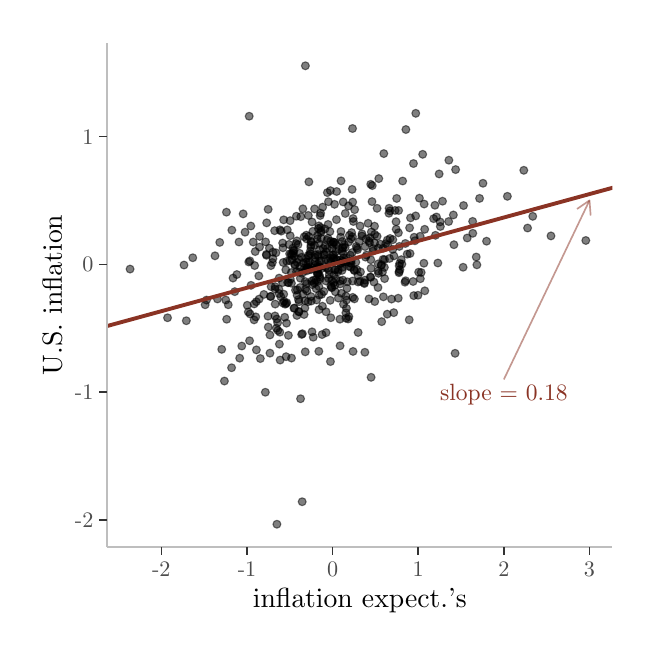
\begin{tikzpicture}[x=1pt,y=1pt]
\definecolor{fillColor}{RGB}{255,255,255}
\path[use as bounding box,fill=fillColor,fill opacity=0.00] (0,0) rectangle (216.81,216.81);
\begin{scope}
\path[clip] (  0.00,  0.00) rectangle (216.81,216.81);
\definecolor{drawColor}{RGB}{255,255,255}
\definecolor{fillColor}{RGB}{255,255,255}

\path[draw=drawColor,line width= 0.6pt,line join=round,line cap=round,fill=fillColor] (  0.00,  0.00) rectangle (216.81,216.81);
\end{scope}
\begin{scope}
\path[clip] ( 28.70, 29.10) rectangle (211.31,211.31);
\definecolor{drawColor}{RGB}{255,255,255}

\path[draw=drawColor,line width= 0.6pt,line join=round] ( 28.70, 38.89) --
	(211.31, 38.89);

\path[draw=drawColor,line width= 0.6pt,line join=round] ( 28.70, 85.08) --
	(211.31, 85.08);

\path[draw=drawColor,line width= 0.6pt,line join=round] ( 28.70,131.28) --
	(211.31,131.28);

\path[draw=drawColor,line width= 0.6pt,line join=round] ( 28.70,177.48) --
	(211.31,177.48);

\path[draw=drawColor,line width= 0.6pt,line join=round] ( 48.30, 29.10) --
	( 48.30,211.31);

\path[draw=drawColor,line width= 0.6pt,line join=round] ( 79.25, 29.10) --
	( 79.25,211.31);

\path[draw=drawColor,line width= 0.6pt,line join=round] (110.19, 29.10) --
	(110.19,211.31);

\path[draw=drawColor,line width= 0.6pt,line join=round] (141.13, 29.10) --
	(141.13,211.31);

\path[draw=drawColor,line width= 0.6pt,line join=round] (172.07, 29.10) --
	(172.07,211.31);

\path[draw=drawColor,line width= 0.6pt,line join=round] (203.01, 29.10) --
	(203.01,211.31);
\definecolor{drawColor}{RGB}{0,0,0}
\definecolor{fillColor}{RGB}{0,0,0}

\path[draw=drawColor,draw opacity=0.50,line width= 0.4pt,line join=round,line cap=round,fill=fillColor,fill opacity=0.50] (164.52,160.58) circle (  1.43);

\path[draw=drawColor,draw opacity=0.50,line width= 0.4pt,line join=round,line cap=round,fill=fillColor,fill opacity=0.50] (148.22,131.77) circle (  1.43);

\path[draw=drawColor,draw opacity=0.50,line width= 0.4pt,line join=round,line cap=round,fill=fillColor,fill opacity=0.50] (138.01,144.47) circle (  1.43);

\path[draw=drawColor,draw opacity=0.50,line width= 0.4pt,line join=round,line cap=round,fill=fillColor,fill opacity=0.50] (162.09,133.94) circle (  1.43);

\path[draw=drawColor,draw opacity=0.50,line width= 0.4pt,line join=round,line cap=round,fill=fillColor,fill opacity=0.50] (135.50,161.40) circle (  1.43);

\path[draw=drawColor,draw opacity=0.50,line width= 0.4pt,line join=round,line cap=round,fill=fillColor,fill opacity=0.50] (123.34,139.71) circle (  1.43);

\path[draw=drawColor,draw opacity=0.50,line width= 0.4pt,line join=round,line cap=round,fill=fillColor,fill opacity=0.50] (139.27,125.09) circle (  1.43);

\path[draw=drawColor,draw opacity=0.50,line width= 0.4pt,line join=round,line cap=round,fill=fillColor,fill opacity=0.50] (143.46,143.95) circle (  1.43);

\path[draw=drawColor,draw opacity=0.50,line width= 0.4pt,line join=round,line cap=round,fill=fillColor,fill opacity=0.50] (160.84,142.51) circle (  1.43);

\path[draw=drawColor,draw opacity=0.50,line width= 0.4pt,line join=round,line cap=round,fill=fillColor,fill opacity=0.50] (173.34,155.87) circle (  1.43);

\path[draw=drawColor,draw opacity=0.50,line width= 0.4pt,line join=round,line cap=round,fill=fillColor,fill opacity=0.50] (158.83,140.81) circle (  1.43);

\path[draw=drawColor,draw opacity=0.50,line width= 0.4pt,line join=round,line cap=round,fill=fillColor,fill opacity=0.50] (165.81,139.65) circle (  1.43);

\path[draw=drawColor,draw opacity=0.50,line width= 0.4pt,line join=round,line cap=round,fill=fillColor,fill opacity=0.50] (189.09,141.56) circle (  1.43);

\path[draw=drawColor,draw opacity=0.50,line width= 0.4pt,line join=round,line cap=round,fill=fillColor,fill opacity=0.50] (182.51,148.64) circle (  1.43);

\path[draw=drawColor,draw opacity=0.50,line width= 0.4pt,line join=round,line cap=round,fill=fillColor,fill opacity=0.50] (180.64,144.41) circle (  1.43);

\path[draw=drawColor,draw opacity=0.50,line width= 0.4pt,line join=round,line cap=round,fill=fillColor,fill opacity=0.50] (160.79,146.81) circle (  1.43);

\path[draw=drawColor,draw opacity=0.50,line width= 0.4pt,line join=round,line cap=round,fill=fillColor,fill opacity=0.50] (134.24,130.73) circle (  1.43);

\path[draw=drawColor,draw opacity=0.50,line width= 0.4pt,line join=round,line cap=round,fill=fillColor,fill opacity=0.50] (123.02,146.12) circle (  1.43);

\path[draw=drawColor,draw opacity=0.50,line width= 0.4pt,line join=round,line cap=round,fill=fillColor,fill opacity=0.50] (163.29,155.12) circle (  1.43);

\path[draw=drawColor,draw opacity=0.50,line width= 0.4pt,line join=round,line cap=round,fill=fillColor,fill opacity=0.50] (141.56,155.20) circle (  1.43);

\path[draw=drawColor,draw opacity=0.50,line width= 0.4pt,line join=round,line cap=round,fill=fillColor,fill opacity=0.50] (157.50,152.54) circle (  1.43);

\path[draw=drawColor,draw opacity=0.50,line width= 0.4pt,line join=round,line cap=round,fill=fillColor,fill opacity=0.50] (131.96,140.20) circle (  1.43);

\path[draw=drawColor,draw opacity=0.50,line width= 0.4pt,line join=round,line cap=round,fill=fillColor,fill opacity=0.50] (149.91,154.10) circle (  1.43);

\path[draw=drawColor,draw opacity=0.50,line width= 0.4pt,line join=round,line cap=round,fill=fillColor,fill opacity=0.50] (100.80,128.92) circle (  1.43);

\path[draw=drawColor,draw opacity=0.50,line width= 0.4pt,line join=round,line cap=round,fill=fillColor,fill opacity=0.50] ( 59.66,133.67) circle (  1.43);

\path[draw=drawColor,draw opacity=0.50,line width= 0.4pt,line join=round,line cap=round,fill=fillColor,fill opacity=0.50] ( 67.69,134.37) circle (  1.43);

\path[draw=drawColor,draw opacity=0.50,line width= 0.4pt,line join=round,line cap=round,fill=fillColor,fill opacity=0.50] ( 71.09, 89.12) circle (  1.43);

\path[draw=drawColor,draw opacity=0.50,line width= 0.4pt,line join=round,line cap=round,fill=fillColor,fill opacity=0.50] ( 99.44,151.36) circle (  1.43);

\path[draw=drawColor,draw opacity=0.50,line width= 0.4pt,line join=round,line cap=round,fill=fillColor,fill opacity=0.50] (111.19,129.32) circle (  1.43);

\path[draw=drawColor,draw opacity=0.50,line width= 0.4pt,line join=round,line cap=round,fill=fillColor,fill opacity=0.50] (118.58,132.08) circle (  1.43);

\path[draw=drawColor,draw opacity=0.50,line width= 0.4pt,line join=round,line cap=round,fill=fillColor,fill opacity=0.50] ( 81.51,139.34) circle (  1.43);

\path[draw=drawColor,draw opacity=0.50,line width= 0.4pt,line join=round,line cap=round,fill=fillColor,fill opacity=0.50] (126.59,122.92) circle (  1.43);

\path[draw=drawColor,draw opacity=0.50,line width= 0.4pt,line join=round,line cap=round,fill=fillColor,fill opacity=0.50] (101.35,117.78) circle (  1.43);

\path[draw=drawColor,draw opacity=0.50,line width= 0.4pt,line join=round,line cap=round,fill=fillColor,fill opacity=0.50] (112.21,129.33) circle (  1.43);

\path[draw=drawColor,draw opacity=0.50,line width= 0.4pt,line join=round,line cap=round,fill=fillColor,fill opacity=0.50] ( 87.54,105.77) circle (  1.43);

\path[draw=drawColor,draw opacity=0.50,line width= 0.4pt,line join=round,line cap=round,fill=fillColor,fill opacity=0.50] (124.07,129.85) circle (  1.43);

\path[draw=drawColor,draw opacity=0.50,line width= 0.4pt,line join=round,line cap=round,fill=fillColor,fill opacity=0.50] (109.92,125.48) circle (  1.43);

\path[draw=drawColor,draw opacity=0.50,line width= 0.4pt,line join=round,line cap=round,fill=fillColor,fill opacity=0.50] (102.13,136.07) circle (  1.43);

\path[draw=drawColor,draw opacity=0.50,line width= 0.4pt,line join=round,line cap=round,fill=fillColor,fill opacity=0.50] ( 80.05,184.81) circle (  1.43);

\path[draw=drawColor,draw opacity=0.50,line width= 0.4pt,line join=round,line cap=round,fill=fillColor,fill opacity=0.50] ( 57.32,110.91) circle (  1.43);

\path[draw=drawColor,draw opacity=0.50,line width= 0.4pt,line join=round,line cap=round,fill=fillColor,fill opacity=0.50] ( 71.82,150.14) circle (  1.43);

\path[draw=drawColor,draw opacity=0.50,line width= 0.4pt,line join=round,line cap=round,fill=fillColor,fill opacity=0.50] ( 70.12,100.58) circle (  1.43);

\path[draw=drawColor,draw opacity=0.50,line width= 0.4pt,line join=round,line cap=round,fill=fillColor,fill opacity=0.50] (100.38,122.31) circle (  1.43);

\path[draw=drawColor,draw opacity=0.50,line width= 0.4pt,line join=round,line cap=round,fill=fillColor,fill opacity=0.50] ( 64.13,116.68) circle (  1.43);

\path[draw=drawColor,draw opacity=0.50,line width= 0.4pt,line join=round,line cap=round,fill=fillColor,fill opacity=0.50] ( 72.48,116.68) circle (  1.43);

\path[draw=drawColor,draw opacity=0.50,line width= 0.4pt,line join=round,line cap=round,fill=fillColor,fill opacity=0.50] ( 81.86,116.98) circle (  1.43);

\path[draw=drawColor,draw opacity=0.50,line width= 0.4pt,line join=round,line cap=round,fill=fillColor,fill opacity=0.50] ( 86.84,112.55) circle (  1.43);

\path[draw=drawColor,draw opacity=0.50,line width= 0.4pt,line join=round,line cap=round,fill=fillColor,fill opacity=0.50] ( 96.02,136.06) circle (  1.43);

\path[draw=drawColor,draw opacity=0.50,line width= 0.4pt,line join=round,line cap=round,fill=fillColor,fill opacity=0.50] ( 77.87,149.52) circle (  1.43);

\path[draw=drawColor,draw opacity=0.50,line width= 0.4pt,line join=round,line cap=round,fill=fillColor,fill opacity=0.50] ( 92.14,138.98) circle (  1.43);

\path[draw=drawColor,draw opacity=0.50,line width= 0.4pt,line join=round,line cap=round,fill=fillColor,fill opacity=0.50] ( 90.96,102.46) circle (  1.43);

\path[draw=drawColor,draw opacity=0.50,line width= 0.4pt,line join=round,line cap=round,fill=fillColor,fill opacity=0.50] (120.09,125.16) circle (  1.43);

\path[draw=drawColor,draw opacity=0.50,line width= 0.4pt,line join=round,line cap=round,fill=fillColor,fill opacity=0.50] ( 95.34, 97.42) circle (  1.43);

\path[draw=drawColor,draw opacity=0.50,line width= 0.4pt,line join=round,line cap=round,fill=fillColor,fill opacity=0.50] (124.52,159.75) circle (  1.43);

\path[draw=drawColor,draw opacity=0.50,line width= 0.4pt,line join=round,line cap=round,fill=fillColor,fill opacity=0.50] (100.30, 99.67) circle (  1.43);

\path[draw=drawColor,draw opacity=0.50,line width= 0.4pt,line join=round,line cap=round,fill=fillColor,fill opacity=0.50] (117.47,119.36) circle (  1.43);

\path[draw=drawColor,draw opacity=0.50,line width= 0.4pt,line join=round,line cap=round,fill=fillColor,fill opacity=0.50] (104.59,140.43) circle (  1.43);

\path[draw=drawColor,draw opacity=0.50,line width= 0.4pt,line join=round,line cap=round,fill=fillColor,fill opacity=0.50] ( 96.78,121.97) circle (  1.43);

\path[draw=drawColor,draw opacity=0.50,line width= 0.4pt,line join=round,line cap=round,fill=fillColor,fill opacity=0.50] ( 73.78,143.65) circle (  1.43);

\path[draw=drawColor,draw opacity=0.50,line width= 0.4pt,line join=round,line cap=round,fill=fillColor,fill opacity=0.50] ( 97.10,148.67) circle (  1.43);

\path[draw=drawColor,draw opacity=0.50,line width= 0.4pt,line join=round,line cap=round,fill=fillColor,fill opacity=0.50] ( 87.55, 99.20) circle (  1.43);

\path[draw=drawColor,draw opacity=0.50,line width= 0.4pt,line join=round,line cap=round,fill=fillColor,fill opacity=0.50] (106.38,105.92) circle (  1.43);

\path[draw=drawColor,draw opacity=0.50,line width= 0.4pt,line join=round,line cap=round,fill=fillColor,fill opacity=0.50] (133.11,146.70) circle (  1.43);

\path[draw=drawColor,draw opacity=0.50,line width= 0.4pt,line join=round,line cap=round,fill=fillColor,fill opacity=0.50] (135.00,132.97) circle (  1.43);

\path[draw=drawColor,draw opacity=0.50,line width= 0.4pt,line join=round,line cap=round,fill=fillColor,fill opacity=0.50] (133.16,143.97) circle (  1.43);

\path[draw=drawColor,draw opacity=0.50,line width= 0.4pt,line join=round,line cap=round,fill=fillColor,fill opacity=0.50] (136.56,125.36) circle (  1.43);

\path[draw=drawColor,draw opacity=0.50,line width= 0.4pt,line join=round,line cap=round,fill=fillColor,fill opacity=0.50] (124.43,153.96) circle (  1.43);

\path[draw=drawColor,draw opacity=0.50,line width= 0.4pt,line join=round,line cap=round,fill=fillColor,fill opacity=0.50] (118.15,151.05) circle (  1.43);

\path[draw=drawColor,draw opacity=0.50,line width= 0.4pt,line join=round,line cap=round,fill=fillColor,fill opacity=0.50] ( 91.16,143.75) circle (  1.43);

\path[draw=drawColor,draw opacity=0.50,line width= 0.4pt,line join=round,line cap=round,fill=fillColor,fill opacity=0.50] ( 93.81,143.73) circle (  1.43);

\path[draw=drawColor,draw opacity=0.50,line width= 0.4pt,line join=round,line cap=round,fill=fillColor,fill opacity=0.50] ( 82.22,135.90) circle (  1.43);

\path[draw=drawColor,draw opacity=0.50,line width= 0.4pt,line join=round,line cap=round,fill=fillColor,fill opacity=0.50] (115.19,115.39) circle (  1.43);

\path[draw=drawColor,draw opacity=0.50,line width= 0.4pt,line join=round,line cap=round,fill=fillColor,fill opacity=0.50] (115.00,132.06) circle (  1.43);

\path[draw=drawColor,draw opacity=0.50,line width= 0.4pt,line join=round,line cap=round,fill=fillColor,fill opacity=0.50] (116.57,134.64) circle (  1.43);

\path[draw=drawColor,draw opacity=0.50,line width= 0.4pt,line join=round,line cap=round,fill=fillColor,fill opacity=0.50] (102.26,130.38) circle (  1.43);

\path[draw=drawColor,draw opacity=0.50,line width= 0.4pt,line join=round,line cap=round,fill=fillColor,fill opacity=0.50] ( 93.62,132.36) circle (  1.43);

\path[draw=drawColor,draw opacity=0.50,line width= 0.4pt,line join=round,line cap=round,fill=fillColor,fill opacity=0.50] ( 92.33,131.97) circle (  1.43);

\path[draw=drawColor,draw opacity=0.50,line width= 0.4pt,line join=round,line cap=round,fill=fillColor,fill opacity=0.50] (113.04,131.88) circle (  1.43);

\path[draw=drawColor,draw opacity=0.50,line width= 0.4pt,line join=round,line cap=round,fill=fillColor,fill opacity=0.50] (110.66,127.46) circle (  1.43);

\path[draw=drawColor,draw opacity=0.50,line width= 0.4pt,line join=round,line cap=round,fill=fillColor,fill opacity=0.50] (108.29,129.78) circle (  1.43);

\path[draw=drawColor,draw opacity=0.50,line width= 0.4pt,line join=round,line cap=round,fill=fillColor,fill opacity=0.50] ( 90.33,110.20) circle (  1.43);

\path[draw=drawColor,draw opacity=0.50,line width= 0.4pt,line join=round,line cap=round,fill=fillColor,fill opacity=0.50] (111.58,147.44) circle (  1.43);

\path[draw=drawColor,draw opacity=0.50,line width= 0.4pt,line join=round,line cap=round,fill=fillColor,fill opacity=0.50] (101.82,134.55) circle (  1.43);

\path[draw=drawColor,draw opacity=0.50,line width= 0.4pt,line join=round,line cap=round,fill=fillColor,fill opacity=0.50] (118.05,118.80) circle (  1.43);

\path[draw=drawColor,draw opacity=0.50,line width= 0.4pt,line join=round,line cap=round,fill=fillColor,fill opacity=0.50] (107.47,138.08) circle (  1.43);

\path[draw=drawColor,draw opacity=0.50,line width= 0.4pt,line join=round,line cap=round,fill=fillColor,fill opacity=0.50] (110.54,134.71) circle (  1.43);

\path[draw=drawColor,draw opacity=0.50,line width= 0.4pt,line join=round,line cap=round,fill=fillColor,fill opacity=0.50] ( 85.36,120.42) circle (  1.43);

\path[draw=drawColor,draw opacity=0.50,line width= 0.4pt,line join=round,line cap=round,fill=fillColor,fill opacity=0.50] ( 94.73,132.64) circle (  1.43);

\path[draw=drawColor,draw opacity=0.50,line width= 0.4pt,line join=round,line cap=round,fill=fillColor,fill opacity=0.50] (104.65,127.86) circle (  1.43);

\path[draw=drawColor,draw opacity=0.50,line width= 0.4pt,line join=round,line cap=round,fill=fillColor,fill opacity=0.50] (123.98,132.95) circle (  1.43);

\path[draw=drawColor,draw opacity=0.50,line width= 0.4pt,line join=round,line cap=round,fill=fillColor,fill opacity=0.50] (107.43,144.03) circle (  1.43);

\path[draw=drawColor,draw opacity=0.50,line width= 0.4pt,line join=round,line cap=round,fill=fillColor,fill opacity=0.50] (121.92,137.73) circle (  1.43);

\path[draw=drawColor,draw opacity=0.50,line width= 0.4pt,line join=round,line cap=round,fill=fillColor,fill opacity=0.50] ( 89.72,135.47) circle (  1.43);

\path[draw=drawColor,draw opacity=0.50,line width= 0.4pt,line join=round,line cap=round,fill=fillColor,fill opacity=0.50] ( 73.68, 93.92) circle (  1.43);

\path[draw=drawColor,draw opacity=0.50,line width= 0.4pt,line join=round,line cap=round,fill=fillColor,fill opacity=0.50] ( 80.18,103.68) circle (  1.43);

\path[draw=drawColor,draw opacity=0.50,line width= 0.4pt,line join=round,line cap=round,fill=fillColor,fill opacity=0.50] (103.57,124.53) circle (  1.43);

\path[draw=drawColor,draw opacity=0.50,line width= 0.4pt,line join=round,line cap=round,fill=fillColor,fill opacity=0.50] (113.10,141.11) circle (  1.43);

\path[draw=drawColor,draw opacity=0.50,line width= 0.4pt,line join=round,line cap=round,fill=fillColor,fill opacity=0.50] (126.65,128.85) circle (  1.43);

\path[draw=drawColor,draw opacity=0.50,line width= 0.4pt,line join=round,line cap=round,fill=fillColor,fill opacity=0.50] (104.72,125.14) circle (  1.43);

\path[draw=drawColor,draw opacity=0.50,line width= 0.4pt,line join=round,line cap=round,fill=fillColor,fill opacity=0.50] (117.95,129.29) circle (  1.43);

\path[draw=drawColor,draw opacity=0.50,line width= 0.4pt,line join=round,line cap=round,fill=fillColor,fill opacity=0.50] (108.52,140.72) circle (  1.43);

\path[draw=drawColor,draw opacity=0.50,line width= 0.4pt,line join=round,line cap=round,fill=fillColor,fill opacity=0.50] (114.12,116.87) circle (  1.43);

\path[draw=drawColor,draw opacity=0.50,line width= 0.4pt,line join=round,line cap=round,fill=fillColor,fill opacity=0.50] (110.99,123.71) circle (  1.43);

\path[draw=drawColor,draw opacity=0.50,line width= 0.4pt,line join=round,line cap=round,fill=fillColor,fill opacity=0.50] (127.82,131.19) circle (  1.43);

\path[draw=drawColor,draw opacity=0.50,line width= 0.4pt,line join=round,line cap=round,fill=fillColor,fill opacity=0.50] (129.38,138.74) circle (  1.43);

\path[draw=drawColor,draw opacity=0.50,line width= 0.4pt,line join=round,line cap=round,fill=fillColor,fill opacity=0.50] (134.04,150.75) circle (  1.43);

\path[draw=drawColor,draw opacity=0.50,line width= 0.4pt,line join=round,line cap=round,fill=fillColor,fill opacity=0.50] (113.23,161.46) circle (  1.43);

\path[draw=drawColor,draw opacity=0.50,line width= 0.4pt,line join=round,line cap=round,fill=fillColor,fill opacity=0.50] ( 86.89,151.17) circle (  1.43);

\path[draw=drawColor,draw opacity=0.50,line width= 0.4pt,line join=round,line cap=round,fill=fillColor,fill opacity=0.50] ( 92.18,117.34) circle (  1.43);

\path[draw=drawColor,draw opacity=0.50,line width= 0.4pt,line join=round,line cap=round,fill=fillColor,fill opacity=0.50] ( 99.92,141.24) circle (  1.43);

\path[draw=drawColor,draw opacity=0.50,line width= 0.4pt,line join=round,line cap=round,fill=fillColor,fill opacity=0.50] ( 92.26,137.27) circle (  1.43);

\path[draw=drawColor,draw opacity=0.50,line width= 0.4pt,line join=round,line cap=round,fill=fillColor,fill opacity=0.50] (105.03,144.22) circle (  1.43);

\path[draw=drawColor,draw opacity=0.50,line width= 0.4pt,line join=round,line cap=round,fill=fillColor,fill opacity=0.50] ( 87.98,123.22) circle (  1.43);

\path[draw=drawColor,draw opacity=0.50,line width= 0.4pt,line join=round,line cap=round,fill=fillColor,fill opacity=0.50] ( 97.69,138.40) circle (  1.43);

\path[draw=drawColor,draw opacity=0.50,line width= 0.4pt,line join=round,line cap=round,fill=fillColor,fill opacity=0.50] ( 87.34,137.12) circle (  1.43);

\path[draw=drawColor,draw opacity=0.50,line width= 0.4pt,line join=round,line cap=round,fill=fillColor,fill opacity=0.50] ( 83.63,118.73) circle (  1.43);

\path[draw=drawColor,draw opacity=0.50,line width= 0.4pt,line join=round,line cap=round,fill=fillColor,fill opacity=0.50] ( 99.13,128.04) circle (  1.43);

\path[draw=drawColor,draw opacity=0.50,line width= 0.4pt,line join=round,line cap=round,fill=fillColor,fill opacity=0.50] (104.09,125.63) circle (  1.43);

\path[draw=drawColor,draw opacity=0.50,line width= 0.4pt,line join=round,line cap=round,fill=fillColor,fill opacity=0.50] (104.04,129.58) circle (  1.43);

\path[draw=drawColor,draw opacity=0.50,line width= 0.4pt,line join=round,line cap=round,fill=fillColor,fill opacity=0.50] (115.99,139.36) circle (  1.43);

\path[draw=drawColor,draw opacity=0.50,line width= 0.4pt,line join=round,line cap=round,fill=fillColor,fill opacity=0.50] (111.41,125.93) circle (  1.43);

\path[draw=drawColor,draw opacity=0.50,line width= 0.4pt,line join=round,line cap=round,fill=fillColor,fill opacity=0.50] (116.88,131.63) circle (  1.43);

\path[draw=drawColor,draw opacity=0.50,line width= 0.4pt,line join=round,line cap=round,fill=fillColor,fill opacity=0.50] (136.47,138.83) circle (  1.43);

\path[draw=drawColor,draw opacity=0.50,line width= 0.4pt,line join=round,line cap=round,fill=fillColor,fill opacity=0.50] (128.98,126.13) circle (  1.43);

\path[draw=drawColor,draw opacity=0.50,line width= 0.4pt,line join=round,line cap=round,fill=fillColor,fill opacity=0.50] (124.72,136.07) circle (  1.43);

\path[draw=drawColor,draw opacity=0.50,line width= 0.4pt,line join=round,line cap=round,fill=fillColor,fill opacity=0.50] (116.91,132.56) circle (  1.43);

\path[draw=drawColor,draw opacity=0.50,line width= 0.4pt,line join=round,line cap=round,fill=fillColor,fill opacity=0.50] (118.06,129.02) circle (  1.43);

\path[draw=drawColor,draw opacity=0.50,line width= 0.4pt,line join=round,line cap=round,fill=fillColor,fill opacity=0.50] (119.83,139.56) circle (  1.43);

\path[draw=drawColor,draw opacity=0.50,line width= 0.4pt,line join=round,line cap=round,fill=fillColor,fill opacity=0.50] (113.79,130.24) circle (  1.43);

\path[draw=drawColor,draw opacity=0.50,line width= 0.4pt,line join=round,line cap=round,fill=fillColor,fill opacity=0.50] (103.63,138.18) circle (  1.43);

\path[draw=drawColor,draw opacity=0.50,line width= 0.4pt,line join=round,line cap=round,fill=fillColor,fill opacity=0.50] (105.33,138.81) circle (  1.43);

\path[draw=drawColor,draw opacity=0.50,line width= 0.4pt,line join=round,line cap=round,fill=fillColor,fill opacity=0.50] (111.69,133.03) circle (  1.43);

\path[draw=drawColor,draw opacity=0.50,line width= 0.4pt,line join=round,line cap=round,fill=fillColor,fill opacity=0.50] (123.67,140.91) circle (  1.43);

\path[draw=drawColor,draw opacity=0.50,line width= 0.4pt,line join=round,line cap=round,fill=fillColor,fill opacity=0.50] (100.92,121.66) circle (  1.43);

\path[draw=drawColor,draw opacity=0.50,line width= 0.4pt,line join=round,line cap=round,fill=fillColor,fill opacity=0.50] (103.83,130.93) circle (  1.43);

\path[draw=drawColor,draw opacity=0.50,line width= 0.4pt,line join=round,line cap=round,fill=fillColor,fill opacity=0.50] ( 89.37,112.64) circle (  1.43);

\path[draw=drawColor,draw opacity=0.50,line width= 0.4pt,line join=round,line cap=round,fill=fillColor,fill opacity=0.50] (106.00,132.57) circle (  1.43);

\path[draw=drawColor,draw opacity=0.50,line width= 0.4pt,line join=round,line cap=round,fill=fillColor,fill opacity=0.50] (110.43,139.32) circle (  1.43);

\path[draw=drawColor,draw opacity=0.50,line width= 0.4pt,line join=round,line cap=round,fill=fillColor,fill opacity=0.50] (110.98,129.39) circle (  1.43);

\path[draw=drawColor,draw opacity=0.50,line width= 0.4pt,line join=round,line cap=round,fill=fillColor,fill opacity=0.50] (101.08,130.14) circle (  1.43);

\path[draw=drawColor,draw opacity=0.50,line width= 0.4pt,line join=round,line cap=round,fill=fillColor,fill opacity=0.50] (109.37,157.91) circle (  1.43);

\path[draw=drawColor,draw opacity=0.50,line width= 0.4pt,line join=round,line cap=round,fill=fillColor,fill opacity=0.50] ( 90.88,120.72) circle (  1.43);

\path[draw=drawColor,draw opacity=0.50,line width= 0.4pt,line join=round,line cap=round,fill=fillColor,fill opacity=0.50] ( 95.53,132.96) circle (  1.43);

\path[draw=drawColor,draw opacity=0.50,line width= 0.4pt,line join=round,line cap=round,fill=fillColor,fill opacity=0.50] ( 89.86,108.22) circle (  1.43);

\path[draw=drawColor,draw opacity=0.50,line width= 0.4pt,line join=round,line cap=round,fill=fillColor,fill opacity=0.50] (104.85,127.92) circle (  1.43);

\path[draw=drawColor,draw opacity=0.50,line width= 0.4pt,line join=round,line cap=round,fill=fillColor,fill opacity=0.50] (114.76,149.66) circle (  1.43);

\path[draw=drawColor,draw opacity=0.50,line width= 0.4pt,line join=round,line cap=round,fill=fillColor,fill opacity=0.50] (104.83,128.09) circle (  1.43);

\path[draw=drawColor,draw opacity=0.50,line width= 0.4pt,line join=round,line cap=round,fill=fillColor,fill opacity=0.50] (128.69,171.31) circle (  1.43);

\path[draw=drawColor,draw opacity=0.50,line width= 0.4pt,line join=round,line cap=round,fill=fillColor,fill opacity=0.50] ( 97.79,133.18) circle (  1.43);

\path[draw=drawColor,draw opacity=0.50,line width= 0.4pt,line join=round,line cap=round,fill=fillColor,fill opacity=0.50] (114.73,137.42) circle (  1.43);

\path[draw=drawColor,draw opacity=0.50,line width= 0.4pt,line join=round,line cap=round,fill=fillColor,fill opacity=0.50] ( 89.37,122.36) circle (  1.43);

\path[draw=drawColor,draw opacity=0.50,line width= 0.4pt,line join=round,line cap=round,fill=fillColor,fill opacity=0.50] ( 83.80,141.39) circle (  1.43);

\path[draw=drawColor,draw opacity=0.50,line width= 0.4pt,line join=round,line cap=round,fill=fillColor,fill opacity=0.50] ( 77.36,101.77) circle (  1.43);

\path[draw=drawColor,draw opacity=0.50,line width= 0.4pt,line join=round,line cap=round,fill=fillColor,fill opacity=0.50] ( 80.29,132.53) circle (  1.43);

\path[draw=drawColor,draw opacity=0.50,line width= 0.4pt,line join=round,line cap=round,fill=fillColor,fill opacity=0.50] ( 80.37,113.36) circle (  1.43);

\path[draw=drawColor,draw opacity=0.50,line width= 0.4pt,line join=round,line cap=round,fill=fillColor,fill opacity=0.50] (101.54,141.38) circle (  1.43);

\path[draw=drawColor,draw opacity=0.50,line width= 0.4pt,line join=round,line cap=round,fill=fillColor,fill opacity=0.50] ( 85.97,139.40) circle (  1.43);

\path[draw=drawColor,draw opacity=0.50,line width= 0.4pt,line join=round,line cap=round,fill=fillColor,fill opacity=0.50] ( 71.91,111.44) circle (  1.43);

\path[draw=drawColor,draw opacity=0.50,line width= 0.4pt,line join=round,line cap=round,fill=fillColor,fill opacity=0.50] ( 83.53,127.10) circle (  1.43);

\path[draw=drawColor,draw opacity=0.50,line width= 0.4pt,line join=round,line cap=round,fill=fillColor,fill opacity=0.50] ( 81.81,111.22) circle (  1.43);

\path[draw=drawColor,draw opacity=0.50,line width= 0.4pt,line join=round,line cap=round,fill=fillColor,fill opacity=0.50] ( 92.13,124.71) circle (  1.43);

\path[draw=drawColor,draw opacity=0.50,line width= 0.4pt,line join=round,line cap=round,fill=fillColor,fill opacity=0.50] (109.54,112.00) circle (  1.43);

\path[draw=drawColor,draw opacity=0.50,line width= 0.4pt,line join=round,line cap=round,fill=fillColor,fill opacity=0.50] (106.60,151.97) circle (  1.43);

\path[draw=drawColor,draw opacity=0.50,line width= 0.4pt,line join=round,line cap=round,fill=fillColor,fill opacity=0.50] ( 64.63,118.38) circle (  1.43);

\path[draw=drawColor,draw opacity=0.50,line width= 0.4pt,line join=round,line cap=round,fill=fillColor,fill opacity=0.50] ( 74.84,121.42) circle (  1.43);

\path[draw=drawColor,draw opacity=0.50,line width= 0.4pt,line join=round,line cap=round,fill=fillColor,fill opacity=0.50] ( 80.63,145.14) circle (  1.43);

\path[draw=drawColor,draw opacity=0.50,line width= 0.4pt,line join=round,line cap=round,fill=fillColor,fill opacity=0.50] ( 78.55,142.90) circle (  1.43);

\path[draw=drawColor,draw opacity=0.50,line width= 0.4pt,line join=round,line cap=round,fill=fillColor,fill opacity=0.50] ( 80.71,123.71) circle (  1.43);

\path[draw=drawColor,draw opacity=0.50,line width= 0.4pt,line join=round,line cap=round,fill=fillColor,fill opacity=0.50] ( 75.59,127.60) circle (  1.43);

\path[draw=drawColor,draw opacity=0.50,line width= 0.4pt,line join=round,line cap=round,fill=fillColor,fill opacity=0.50] ( 95.92,135.34) circle (  1.43);

\path[draw=drawColor,draw opacity=0.50,line width= 0.4pt,line join=round,line cap=round,fill=fillColor,fill opacity=0.50] ( 83.80,137.55) circle (  1.43);

\path[draw=drawColor,draw opacity=0.50,line width= 0.4pt,line join=round,line cap=round,fill=fillColor,fill opacity=0.50] ( 94.29,124.69) circle (  1.43);

\path[draw=drawColor,draw opacity=0.50,line width= 0.4pt,line join=round,line cap=round,fill=fillColor,fill opacity=0.50] ( 96.51,131.26) circle (  1.43);

\path[draw=drawColor,draw opacity=0.50,line width= 0.4pt,line join=round,line cap=round,fill=fillColor,fill opacity=0.50] ( 86.36,146.28) circle (  1.43);

\path[draw=drawColor,draw opacity=0.50,line width= 0.4pt,line join=round,line cap=round,fill=fillColor,fill opacity=0.50] ( 89.44,116.93) circle (  1.43);

\path[draw=drawColor,draw opacity=0.50,line width= 0.4pt,line join=round,line cap=round,fill=fillColor,fill opacity=0.50] ( 82.03,130.85) circle (  1.43);

\path[draw=drawColor,draw opacity=0.50,line width= 0.4pt,line join=round,line cap=round,fill=fillColor,fill opacity=0.50] ( 92.50,147.37) circle (  1.43);

\path[draw=drawColor,draw opacity=0.50,line width= 0.4pt,line join=round,line cap=round,fill=fillColor,fill opacity=0.50] ( 89.43,123.23) circle (  1.43);

\path[draw=drawColor,draw opacity=0.50,line width= 0.4pt,line join=round,line cap=round,fill=fillColor,fill opacity=0.50] (109.53,123.55) circle (  1.43);

\path[draw=drawColor,draw opacity=0.50,line width= 0.4pt,line join=round,line cap=round,fill=fillColor,fill opacity=0.50] ( 91.60,143.29) circle (  1.43);

\path[draw=drawColor,draw opacity=0.50,line width= 0.4pt,line join=round,line cap=round,fill=fillColor,fill opacity=0.50] (101.91,129.55) circle (  1.43);

\path[draw=drawColor,draw opacity=0.50,line width= 0.4pt,line join=round,line cap=round,fill=fillColor,fill opacity=0.50] (113.36,120.84) circle (  1.43);

\path[draw=drawColor,draw opacity=0.50,line width= 0.4pt,line join=round,line cap=round,fill=fillColor,fill opacity=0.50] (107.65,130.35) circle (  1.43);

\path[draw=drawColor,draw opacity=0.50,line width= 0.4pt,line join=round,line cap=round,fill=fillColor,fill opacity=0.50] (111.42,132.94) circle (  1.43);

\path[draw=drawColor,draw opacity=0.50,line width= 0.4pt,line join=round,line cap=round,fill=fillColor,fill opacity=0.50] (105.52,126.72) circle (  1.43);

\path[draw=drawColor,draw opacity=0.50,line width= 0.4pt,line join=round,line cap=round,fill=fillColor,fill opacity=0.50] (108.66,132.57) circle (  1.43);

\path[draw=drawColor,draw opacity=0.50,line width= 0.4pt,line join=round,line cap=round,fill=fillColor,fill opacity=0.50] ( 98.37,130.43) circle (  1.43);

\path[draw=drawColor,draw opacity=0.50,line width= 0.4pt,line join=round,line cap=round,fill=fillColor,fill opacity=0.50] ( 96.31,134.21) circle (  1.43);

\path[draw=drawColor,draw opacity=0.50,line width= 0.4pt,line join=round,line cap=round,fill=fillColor,fill opacity=0.50] ( 97.30,112.81) circle (  1.43);

\path[draw=drawColor,draw opacity=0.50,line width= 0.4pt,line join=round,line cap=round,fill=fillColor,fill opacity=0.50] (103.07,143.22) circle (  1.43);

\path[draw=drawColor,draw opacity=0.50,line width= 0.4pt,line join=round,line cap=round,fill=fillColor,fill opacity=0.50] (112.97,132.81) circle (  1.43);

\path[draw=drawColor,draw opacity=0.50,line width= 0.4pt,line join=round,line cap=round,fill=fillColor,fill opacity=0.50] (105.28,114.92) circle (  1.43);

\path[draw=drawColor,draw opacity=0.50,line width= 0.4pt,line join=round,line cap=round,fill=fillColor,fill opacity=0.50] (114.12,135.07) circle (  1.43);

\path[draw=drawColor,draw opacity=0.50,line width= 0.4pt,line join=round,line cap=round,fill=fillColor,fill opacity=0.50] (102.44,139.63) circle (  1.43);

\path[draw=drawColor,draw opacity=0.50,line width= 0.4pt,line join=round,line cap=round,fill=fillColor,fill opacity=0.50] (101.34,134.52) circle (  1.43);

\path[draw=drawColor,draw opacity=0.50,line width= 0.4pt,line join=round,line cap=round,fill=fillColor,fill opacity=0.50] (119.21,136.59) circle (  1.43);

\path[draw=drawColor,draw opacity=0.50,line width= 0.4pt,line join=round,line cap=round,fill=fillColor,fill opacity=0.50] (116.77,130.26) circle (  1.43);

\path[draw=drawColor,draw opacity=0.50,line width= 0.4pt,line join=round,line cap=round,fill=fillColor,fill opacity=0.50] ( 98.01,114.11) circle (  1.43);

\path[draw=drawColor,draw opacity=0.50,line width= 0.4pt,line join=round,line cap=round,fill=fillColor,fill opacity=0.50] (123.54,139.11) circle (  1.43);

\path[draw=drawColor,draw opacity=0.50,line width= 0.4pt,line join=round,line cap=round,fill=fillColor,fill opacity=0.50] (105.40,127.43) circle (  1.43);

\path[draw=drawColor,draw opacity=0.50,line width= 0.4pt,line join=round,line cap=round,fill=fillColor,fill opacity=0.50] (113.21,143.16) circle (  1.43);

\path[draw=drawColor,draw opacity=0.50,line width= 0.4pt,line join=round,line cap=round,fill=fillColor,fill opacity=0.50] (105.24,123.25) circle (  1.43);

\path[draw=drawColor,draw opacity=0.50,line width= 0.4pt,line join=round,line cap=round,fill=fillColor,fill opacity=0.50] (113.60,129.11) circle (  1.43);

\path[draw=drawColor,draw opacity=0.50,line width= 0.4pt,line join=round,line cap=round,fill=fillColor,fill opacity=0.50] (117.58,147.86) circle (  1.43);

\path[draw=drawColor,draw opacity=0.50,line width= 0.4pt,line join=round,line cap=round,fill=fillColor,fill opacity=0.50] (107.02,121.48) circle (  1.43);

\path[draw=drawColor,draw opacity=0.50,line width= 0.4pt,line join=round,line cap=round,fill=fillColor,fill opacity=0.50] (104.63,129.86) circle (  1.43);

\path[draw=drawColor,draw opacity=0.50,line width= 0.4pt,line join=round,line cap=round,fill=fillColor,fill opacity=0.50] (104.23,122.50) circle (  1.43);

\path[draw=drawColor,draw opacity=0.50,line width= 0.4pt,line join=round,line cap=round,fill=fillColor,fill opacity=0.50] (107.74,125.29) circle (  1.43);

\path[draw=drawColor,draw opacity=0.50,line width= 0.4pt,line join=round,line cap=round,fill=fillColor,fill opacity=0.50] (116.04,130.59) circle (  1.43);

\path[draw=drawColor,draw opacity=0.50,line width= 0.4pt,line join=round,line cap=round,fill=fillColor,fill opacity=0.50] (109.48,139.63) circle (  1.43);

\path[draw=drawColor,draw opacity=0.50,line width= 0.4pt,line join=round,line cap=round,fill=fillColor,fill opacity=0.50] ( 97.87,118.55) circle (  1.43);

\path[draw=drawColor,draw opacity=0.50,line width= 0.4pt,line join=round,line cap=round,fill=fillColor,fill opacity=0.50] ( 97.37,132.00) circle (  1.43);

\path[draw=drawColor,draw opacity=0.50,line width= 0.4pt,line join=round,line cap=round,fill=fillColor,fill opacity=0.50] (105.99,142.86) circle (  1.43);

\path[draw=drawColor,draw opacity=0.50,line width= 0.4pt,line join=round,line cap=round,fill=fillColor,fill opacity=0.50] ( 97.36,120.13) circle (  1.43);

\path[draw=drawColor,draw opacity=0.50,line width= 0.4pt,line join=round,line cap=round,fill=fillColor,fill opacity=0.50] (108.15,139.99) circle (  1.43);

\path[draw=drawColor,draw opacity=0.50,line width= 0.4pt,line join=round,line cap=round,fill=fillColor,fill opacity=0.50] (108.73,126.18) circle (  1.43);

\path[draw=drawColor,draw opacity=0.50,line width= 0.4pt,line join=round,line cap=round,fill=fillColor,fill opacity=0.50] (126.65,131.46) circle (  1.43);

\path[draw=drawColor,draw opacity=0.50,line width= 0.4pt,line join=round,line cap=round,fill=fillColor,fill opacity=0.50] (100.02,129.99) circle (  1.43);

\path[draw=drawColor,draw opacity=0.50,line width= 0.4pt,line join=round,line cap=round,fill=fillColor,fill opacity=0.50] (110.60,133.33) circle (  1.43);

\path[draw=drawColor,draw opacity=0.50,line width= 0.4pt,line join=round,line cap=round,fill=fillColor,fill opacity=0.50] (112.90,125.30) circle (  1.43);

\path[draw=drawColor,draw opacity=0.50,line width= 0.4pt,line join=round,line cap=round,fill=fillColor,fill opacity=0.50] (117.37,141.26) circle (  1.43);

\path[draw=drawColor,draw opacity=0.50,line width= 0.4pt,line join=round,line cap=round,fill=fillColor,fill opacity=0.50] (109.01,127.65) circle (  1.43);

\path[draw=drawColor,draw opacity=0.50,line width= 0.4pt,line join=round,line cap=round,fill=fillColor,fill opacity=0.50] (102.43,139.36) circle (  1.43);

\path[draw=drawColor,draw opacity=0.50,line width= 0.4pt,line join=round,line cap=round,fill=fillColor,fill opacity=0.50] (101.39,132.04) circle (  1.43);

\path[draw=drawColor,draw opacity=0.50,line width= 0.4pt,line join=round,line cap=round,fill=fillColor,fill opacity=0.50] ( 99.87,113.17) circle (  1.43);

\path[draw=drawColor,draw opacity=0.50,line width= 0.4pt,line join=round,line cap=round,fill=fillColor,fill opacity=0.50] (110.61,139.22) circle (  1.43);

\path[draw=drawColor,draw opacity=0.50,line width= 0.4pt,line join=round,line cap=round,fill=fillColor,fill opacity=0.50] ( 96.22,115.43) circle (  1.43);

\path[draw=drawColor,draw opacity=0.50,line width= 0.4pt,line join=round,line cap=round,fill=fillColor,fill opacity=0.50] (111.17,121.38) circle (  1.43);

\path[draw=drawColor,draw opacity=0.50,line width= 0.4pt,line join=round,line cap=round,fill=fillColor,fill opacity=0.50] (123.79,126.72) circle (  1.43);

\path[draw=drawColor,draw opacity=0.50,line width= 0.4pt,line join=round,line cap=round,fill=fillColor,fill opacity=0.50] (116.41,131.88) circle (  1.43);

\path[draw=drawColor,draw opacity=0.50,line width= 0.4pt,line join=round,line cap=round,fill=fillColor,fill opacity=0.50] (102.62,125.23) circle (  1.43);

\path[draw=drawColor,draw opacity=0.50,line width= 0.4pt,line join=round,line cap=round,fill=fillColor,fill opacity=0.50] (108.25,137.00) circle (  1.43);

\path[draw=drawColor,draw opacity=0.50,line width= 0.4pt,line join=round,line cap=round,fill=fillColor,fill opacity=0.50] (109.92,122.86) circle (  1.43);

\path[draw=drawColor,draw opacity=0.50,line width= 0.4pt,line join=round,line cap=round,fill=fillColor,fill opacity=0.50] (105.72,126.05) circle (  1.43);

\path[draw=drawColor,draw opacity=0.50,line width= 0.4pt,line join=round,line cap=round,fill=fillColor,fill opacity=0.50] (109.73,123.00) circle (  1.43);

\path[draw=drawColor,draw opacity=0.50,line width= 0.4pt,line join=round,line cap=round,fill=fillColor,fill opacity=0.50] (112.86,124.18) circle (  1.43);

\path[draw=drawColor,draw opacity=0.50,line width= 0.4pt,line join=round,line cap=round,fill=fillColor,fill opacity=0.50] (102.35,129.39) circle (  1.43);

\path[draw=drawColor,draw opacity=0.50,line width= 0.4pt,line join=round,line cap=round,fill=fillColor,fill opacity=0.50] ( 92.52,120.51) circle (  1.43);

\path[draw=drawColor,draw opacity=0.50,line width= 0.4pt,line join=round,line cap=round,fill=fillColor,fill opacity=0.50] (104.74,130.39) circle (  1.43);

\path[draw=drawColor,draw opacity=0.50,line width= 0.4pt,line join=round,line cap=round,fill=fillColor,fill opacity=0.50] ( 99.56,131.75) circle (  1.43);

\path[draw=drawColor,draw opacity=0.50,line width= 0.4pt,line join=round,line cap=round,fill=fillColor,fill opacity=0.50] (111.36,138.52) circle (  1.43);

\path[draw=drawColor,draw opacity=0.50,line width= 0.4pt,line join=round,line cap=round,fill=fillColor,fill opacity=0.50] (106.22,120.45) circle (  1.43);

\path[draw=drawColor,draw opacity=0.50,line width= 0.4pt,line join=round,line cap=round,fill=fillColor,fill opacity=0.50] (102.36,138.22) circle (  1.43);

\path[draw=drawColor,draw opacity=0.50,line width= 0.4pt,line join=round,line cap=round,fill=fillColor,fill opacity=0.50] ( 91.47,119.59) circle (  1.43);

\path[draw=drawColor,draw opacity=0.50,line width= 0.4pt,line join=round,line cap=round,fill=fillColor,fill opacity=0.50] ( 95.31,124.45) circle (  1.43);

\path[draw=drawColor,draw opacity=0.50,line width= 0.4pt,line join=round,line cap=round,fill=fillColor,fill opacity=0.50] ( 98.21,135.30) circle (  1.43);

\path[draw=drawColor,draw opacity=0.50,line width= 0.4pt,line join=round,line cap=round,fill=fillColor,fill opacity=0.50] ( 94.90,125.97) circle (  1.43);

\path[draw=drawColor,draw opacity=0.50,line width= 0.4pt,line join=round,line cap=round,fill=fillColor,fill opacity=0.50] (102.13,135.15) circle (  1.43);

\path[draw=drawColor,draw opacity=0.50,line width= 0.4pt,line join=round,line cap=round,fill=fillColor,fill opacity=0.50] ( 97.15,128.64) circle (  1.43);

\path[draw=drawColor,draw opacity=0.50,line width= 0.4pt,line join=round,line cap=round,fill=fillColor,fill opacity=0.50] ( 98.07,128.49) circle (  1.43);

\path[draw=drawColor,draw opacity=0.50,line width= 0.4pt,line join=round,line cap=round,fill=fillColor,fill opacity=0.50] (100.61,132.14) circle (  1.43);

\path[draw=drawColor,draw opacity=0.50,line width= 0.4pt,line join=round,line cap=round,fill=fillColor,fill opacity=0.50] (110.88,152.98) circle (  1.43);

\path[draw=drawColor,draw opacity=0.50,line width= 0.4pt,line join=round,line cap=round,fill=fillColor,fill opacity=0.50] ( 90.39,107.39) circle (  1.43);

\path[draw=drawColor,draw opacity=0.50,line width= 0.4pt,line join=round,line cap=round,fill=fillColor,fill opacity=0.50] (103.86,132.23) circle (  1.43);

\path[draw=drawColor,draw opacity=0.50,line width= 0.4pt,line join=round,line cap=round,fill=fillColor,fill opacity=0.50] ( 96.96,138.78) circle (  1.43);

\path[draw=drawColor,draw opacity=0.50,line width= 0.4pt,line join=round,line cap=round,fill=fillColor,fill opacity=0.50] (100.53,129.40) circle (  1.43);

\path[draw=drawColor,draw opacity=0.50,line width= 0.4pt,line join=round,line cap=round,fill=fillColor,fill opacity=0.50] (105.85,144.57) circle (  1.43);

\path[draw=drawColor,draw opacity=0.50,line width= 0.4pt,line join=round,line cap=round,fill=fillColor,fill opacity=0.50] (100.27,118.13) circle (  1.43);

\path[draw=drawColor,draw opacity=0.50,line width= 0.4pt,line join=round,line cap=round,fill=fillColor,fill opacity=0.50] ( 96.28,136.36) circle (  1.43);

\path[draw=drawColor,draw opacity=0.50,line width= 0.4pt,line join=round,line cap=round,fill=fillColor,fill opacity=0.50] (106.19,129.77) circle (  1.43);

\path[draw=drawColor,draw opacity=0.50,line width= 0.4pt,line join=round,line cap=round,fill=fillColor,fill opacity=0.50] (103.84,133.76) circle (  1.43);

\path[draw=drawColor,draw opacity=0.50,line width= 0.4pt,line join=round,line cap=round,fill=fillColor,fill opacity=0.50] (102.76,146.60) circle (  1.43);

\path[draw=drawColor,draw opacity=0.50,line width= 0.4pt,line join=round,line cap=round,fill=fillColor,fill opacity=0.50] (105.24,145.19) circle (  1.43);

\path[draw=drawColor,draw opacity=0.50,line width= 0.4pt,line join=round,line cap=round,fill=fillColor,fill opacity=0.50] ( 85.88, 85.07) circle (  1.43);

\path[draw=drawColor,draw opacity=0.50,line width= 0.4pt,line join=round,line cap=round,fill=fillColor,fill opacity=0.50] (108.30,157.22) circle (  1.43);

\path[draw=drawColor,draw opacity=0.50,line width= 0.4pt,line join=round,line cap=round,fill=fillColor,fill opacity=0.50] ( 98.69,148.51) circle (  1.43);

\path[draw=drawColor,draw opacity=0.50,line width= 0.4pt,line join=round,line cap=round,fill=fillColor,fill opacity=0.50] ( 93.53,110.03) circle (  1.43);

\path[draw=drawColor,draw opacity=0.50,line width= 0.4pt,line join=round,line cap=round,fill=fillColor,fill opacity=0.50] ( 98.53,126.26) circle (  1.43);

\path[draw=drawColor,draw opacity=0.50,line width= 0.4pt,line join=round,line cap=round,fill=fillColor,fill opacity=0.50] (110.99,139.22) circle (  1.43);

\path[draw=drawColor,draw opacity=0.50,line width= 0.4pt,line join=round,line cap=round,fill=fillColor,fill opacity=0.50] (119.41,124.91) circle (  1.43);

\path[draw=drawColor,draw opacity=0.50,line width= 0.4pt,line join=round,line cap=round,fill=fillColor,fill opacity=0.50] (105.48,130.37) circle (  1.43);

\path[draw=drawColor,draw opacity=0.50,line width= 0.4pt,line join=round,line cap=round,fill=fillColor,fill opacity=0.50] ( 93.27,129.30) circle (  1.43);

\path[draw=drawColor,draw opacity=0.50,line width= 0.4pt,line join=round,line cap=round,fill=fillColor,fill opacity=0.50] (109.22,143.14) circle (  1.43);

\path[draw=drawColor,draw opacity=0.50,line width= 0.4pt,line join=round,line cap=round,fill=fillColor,fill opacity=0.50] ( 79.74,114.08) circle (  1.43);

\path[draw=drawColor,draw opacity=0.50,line width= 0.4pt,line join=round,line cap=round,fill=fillColor,fill opacity=0.50] ( 89.99,111.53) circle (  1.43);

\path[draw=drawColor,draw opacity=0.50,line width= 0.4pt,line join=round,line cap=round,fill=fillColor,fill opacity=0.50] (115.93,152.38) circle (  1.43);

\path[draw=drawColor,draw opacity=0.50,line width= 0.4pt,line join=round,line cap=round,fill=fillColor,fill opacity=0.50] (111.30,135.81) circle (  1.43);

\path[draw=drawColor,draw opacity=0.50,line width= 0.4pt,line join=round,line cap=round,fill=fillColor,fill opacity=0.50] (107.82,106.61) circle (  1.43);

\path[draw=drawColor,draw opacity=0.50,line width= 0.4pt,line join=round,line cap=round,fill=fillColor,fill opacity=0.50] ( 87.68,119.70) circle (  1.43);

\path[draw=drawColor,draw opacity=0.50,line width= 0.4pt,line join=round,line cap=round,fill=fillColor,fill opacity=0.50] ( 94.42,138.49) circle (  1.43);

\path[draw=drawColor,draw opacity=0.50,line width= 0.4pt,line join=round,line cap=round,fill=fillColor,fill opacity=0.50] ( 99.47,120.51) circle (  1.43);

\path[draw=drawColor,draw opacity=0.50,line width= 0.4pt,line join=round,line cap=round,fill=fillColor,fill opacity=0.50] ( 50.54,111.98) circle (  1.43);

\path[draw=drawColor,draw opacity=0.50,line width= 0.4pt,line join=round,line cap=round,fill=fillColor,fill opacity=0.50] ( 37.00,129.58) circle (  1.43);

\path[draw=drawColor,draw opacity=0.50,line width= 0.4pt,line join=round,line cap=round,fill=fillColor,fill opacity=0.50] ( 68.58,118.77) circle (  1.43);

\path[draw=drawColor,draw opacity=0.50,line width= 0.4pt,line join=round,line cap=round,fill=fillColor,fill opacity=0.50] ( 79.35,116.50) circle (  1.43);

\path[draw=drawColor,draw opacity=0.50,line width= 0.4pt,line join=round,line cap=round,fill=fillColor,fill opacity=0.50] ( 95.46,134.71) circle (  1.43);

\path[draw=drawColor,draw opacity=0.50,line width= 0.4pt,line join=round,line cap=round,fill=fillColor,fill opacity=0.50] (110.11,138.51) circle (  1.43);

\path[draw=drawColor,draw opacity=0.50,line width= 0.4pt,line join=round,line cap=round,fill=fillColor,fill opacity=0.50] (106.78,137.02) circle (  1.43);

\path[draw=drawColor,draw opacity=0.50,line width= 0.4pt,line join=round,line cap=round,fill=fillColor,fill opacity=0.50] ( 99.26,106.22) circle (  1.43);

\path[draw=drawColor,draw opacity=0.50,line width= 0.4pt,line join=round,line cap=round,fill=fillColor,fill opacity=0.50] (110.25,133.73) circle (  1.43);

\path[draw=drawColor,draw opacity=0.50,line width= 0.4pt,line join=round,line cap=round,fill=fillColor,fill opacity=0.50] (101.42,148.96) circle (  1.43);

\path[draw=drawColor,draw opacity=0.50,line width= 0.4pt,line join=round,line cap=round,fill=fillColor,fill opacity=0.50] ( 88.41,131.96) circle (  1.43);

\path[draw=drawColor,draw opacity=0.50,line width= 0.4pt,line join=round,line cap=round,fill=fillColor,fill opacity=0.50] ( 96.38,115.47) circle (  1.43);

\path[draw=drawColor,draw opacity=0.50,line width= 0.4pt,line join=round,line cap=round,fill=fillColor,fill opacity=0.50] (101.62,161.10) circle (  1.43);

\path[draw=drawColor,draw opacity=0.50,line width= 0.4pt,line join=round,line cap=round,fill=fillColor,fill opacity=0.50] ( 74.20,126.33) circle (  1.43);

\path[draw=drawColor,draw opacity=0.50,line width= 0.4pt,line join=round,line cap=round,fill=fillColor,fill opacity=0.50] ( 76.36,139.36) circle (  1.43);

\path[draw=drawColor,draw opacity=0.50,line width= 0.4pt,line join=round,line cap=round,fill=fillColor,fill opacity=0.50] ( 69.41,139.22) circle (  1.43);

\path[draw=drawColor,draw opacity=0.50,line width= 0.4pt,line join=round,line cap=round,fill=fillColor,fill opacity=0.50] ( 89.25,143.45) circle (  1.43);

\path[draw=drawColor,draw opacity=0.50,line width= 0.4pt,line join=round,line cap=round,fill=fillColor,fill opacity=0.50] ( 98.09,117.79) circle (  1.43);

\path[draw=drawColor,draw opacity=0.50,line width= 0.4pt,line join=round,line cap=round,fill=fillColor,fill opacity=0.50] ( 76.61, 97.38) circle (  1.43);

\path[draw=drawColor,draw opacity=0.50,line width= 0.4pt,line join=round,line cap=round,fill=fillColor,fill opacity=0.50] ( 95.84,137.15) circle (  1.43);

\path[draw=drawColor,draw opacity=0.50,line width= 0.4pt,line join=round,line cap=round,fill=fillColor,fill opacity=0.50] ( 88.63,133.34) circle (  1.43);

\path[draw=drawColor,draw opacity=0.50,line width= 0.4pt,line join=round,line cap=round,fill=fillColor,fill opacity=0.50] ( 79.90,132.14) circle (  1.43);

\path[draw=drawColor,draw opacity=0.50,line width= 0.4pt,line join=round,line cap=round,fill=fillColor,fill opacity=0.50] ( 88.62,135.70) circle (  1.43);

\path[draw=drawColor,draw opacity=0.50,line width= 0.4pt,line join=round,line cap=round,fill=fillColor,fill opacity=0.50] (104.86,134.84) circle (  1.43);

\path[draw=drawColor,draw opacity=0.50,line width= 0.4pt,line join=round,line cap=round,fill=fillColor,fill opacity=0.50] ( 92.89,112.17) circle (  1.43);

\path[draw=drawColor,draw opacity=0.50,line width= 0.4pt,line join=round,line cap=round,fill=fillColor,fill opacity=0.50] (105.00,134.32) circle (  1.43);

\path[draw=drawColor,draw opacity=0.50,line width= 0.4pt,line join=round,line cap=round,fill=fillColor,fill opacity=0.50] ( 94.66,135.11) circle (  1.43);

\path[draw=drawColor,draw opacity=0.50,line width= 0.4pt,line join=round,line cap=round,fill=fillColor,fill opacity=0.50] ( 90.87,126.32) circle (  1.43);

\path[draw=drawColor,draw opacity=0.50,line width= 0.4pt,line join=round,line cap=round,fill=fillColor,fill opacity=0.50] (100.16,115.49) circle (  1.43);

\path[draw=drawColor,draw opacity=0.50,line width= 0.4pt,line join=round,line cap=round,fill=fillColor,fill opacity=0.50] (122.33,140.51) circle (  1.43);

\path[draw=drawColor,draw opacity=0.50,line width= 0.4pt,line join=round,line cap=round,fill=fillColor,fill opacity=0.50] (130.60,151.55) circle (  1.43);

\path[draw=drawColor,draw opacity=0.50,line width= 0.4pt,line join=round,line cap=round,fill=fillColor,fill opacity=0.50] (120.12,145.15) circle (  1.43);

\path[draw=drawColor,draw opacity=0.50,line width= 0.4pt,line join=round,line cap=round,fill=fillColor,fill opacity=0.50] (105.45,132.39) circle (  1.43);

\path[draw=drawColor,draw opacity=0.50,line width= 0.4pt,line join=round,line cap=round,fill=fillColor,fill opacity=0.50] ( 92.63,117.87) circle (  1.43);

\path[draw=drawColor,draw opacity=0.50,line width= 0.4pt,line join=round,line cap=round,fill=fillColor,fill opacity=0.50] ( 87.90,119.67) circle (  1.43);

\path[draw=drawColor,draw opacity=0.50,line width= 0.4pt,line join=round,line cap=round,fill=fillColor,fill opacity=0.50] (102.34,137.51) circle (  1.43);

\path[draw=drawColor,draw opacity=0.50,line width= 0.4pt,line join=round,line cap=round,fill=fillColor,fill opacity=0.50] (111.64,157.61) circle (  1.43);

\path[draw=drawColor,draw opacity=0.50,line width= 0.4pt,line join=round,line cap=round,fill=fillColor,fill opacity=0.50] ( 86.30,134.56) circle (  1.43);

\path[draw=drawColor,draw opacity=0.50,line width= 0.4pt,line join=round,line cap=round,fill=fillColor,fill opacity=0.50] ( 82.42,112.31) circle (  1.43);

\path[draw=drawColor,draw opacity=0.50,line width= 0.4pt,line join=round,line cap=round,fill=fillColor,fill opacity=0.50] ( 93.61,117.42) circle (  1.43);

\path[draw=drawColor,draw opacity=0.50,line width= 0.4pt,line join=round,line cap=round,fill=fillColor,fill opacity=0.50] (105.87,149.78) circle (  1.43);

\path[draw=drawColor,draw opacity=0.50,line width= 0.4pt,line join=round,line cap=round,fill=fillColor,fill opacity=0.50] (112.09,128.60) circle (  1.43);

\path[draw=drawColor,draw opacity=0.50,line width= 0.4pt,line join=round,line cap=round,fill=fillColor,fill opacity=0.50] (117.28,135.55) circle (  1.43);

\path[draw=drawColor,draw opacity=0.50,line width= 0.4pt,line join=round,line cap=round,fill=fillColor,fill opacity=0.50] (103.19,104.95) circle (  1.43);

\path[draw=drawColor,draw opacity=0.50,line width= 0.4pt,line join=round,line cap=round,fill=fillColor,fill opacity=0.50] (126.77,128.05) circle (  1.43);

\path[draw=drawColor,draw opacity=0.50,line width= 0.4pt,line join=round,line cap=round,fill=fillColor,fill opacity=0.50] (117.24,158.37) circle (  1.43);

\path[draw=drawColor,draw opacity=0.50,line width= 0.4pt,line join=round,line cap=round,fill=fillColor,fill opacity=0.50] (104.73,141.69) circle (  1.43);

\path[draw=drawColor,draw opacity=0.50,line width= 0.4pt,line join=round,line cap=round,fill=fillColor,fill opacity=0.50] (142.74,171.05) circle (  1.43);

\path[draw=drawColor,draw opacity=0.50,line width= 0.4pt,line join=round,line cap=round,fill=fillColor,fill opacity=0.50] (124.09, 90.47) circle (  1.43);

\path[draw=drawColor,draw opacity=0.50,line width= 0.4pt,line join=round,line cap=round,fill=fillColor,fill opacity=0.50] (112.88,101.86) circle (  1.43);

\path[draw=drawColor,draw opacity=0.50,line width= 0.4pt,line join=round,line cap=round,fill=fillColor,fill opacity=0.50] (126.25,151.54) circle (  1.43);

\path[draw=drawColor,draw opacity=0.50,line width= 0.4pt,line join=round,line cap=round,fill=fillColor,fill opacity=0.50] (108.69,153.91) circle (  1.43);

\path[draw=drawColor,draw opacity=0.50,line width= 0.4pt,line join=round,line cap=round,fill=fillColor,fill opacity=0.50] ( 91.23, 96.70) circle (  1.43);

\path[draw=drawColor,draw opacity=0.50,line width= 0.4pt,line join=round,line cap=round,fill=fillColor,fill opacity=0.50] (110.24,134.59) circle (  1.43);

\path[draw=drawColor,draw opacity=0.50,line width= 0.4pt,line join=round,line cap=round,fill=fillColor,fill opacity=0.50] (126.26,141.41) circle (  1.43);

\path[draw=drawColor,draw opacity=0.50,line width= 0.4pt,line join=round,line cap=round,fill=fillColor,fill opacity=0.50] (130.97,140.63) circle (  1.43);

\path[draw=drawColor,draw opacity=0.50,line width= 0.4pt,line join=round,line cap=round,fill=fillColor,fill opacity=0.50] (113.87,132.52) circle (  1.43);

\path[draw=drawColor,draw opacity=0.50,line width= 0.4pt,line join=round,line cap=round,fill=fillColor,fill opacity=0.50] ( 93.93,124.71) circle (  1.43);

\path[draw=drawColor,draw opacity=0.50,line width= 0.4pt,line join=round,line cap=round,fill=fillColor,fill opacity=0.50] (121.89,125.59) circle (  1.43);

\path[draw=drawColor,draw opacity=0.50,line width= 0.4pt,line join=round,line cap=round,fill=fillColor,fill opacity=0.50] ( 99.19, 45.51) circle (  1.43);

\path[draw=drawColor,draw opacity=0.50,line width= 0.4pt,line join=round,line cap=round,fill=fillColor,fill opacity=0.50] (149.03,146.62) circle (  1.43);

\path[draw=drawColor,draw opacity=0.50,line width= 0.4pt,line join=round,line cap=round,fill=fillColor,fill opacity=0.50] (133.34,155.10) circle (  1.43);

\path[draw=drawColor,draw opacity=0.50,line width= 0.4pt,line join=round,line cap=round,fill=fillColor,fill opacity=0.50] (119.01,137.14) circle (  1.43);

\path[draw=drawColor,draw opacity=0.50,line width= 0.4pt,line join=round,line cap=round,fill=fillColor,fill opacity=0.50] (105.22, 99.86) circle (  1.43);

\path[draw=drawColor,draw opacity=0.50,line width= 0.4pt,line join=round,line cap=round,fill=fillColor,fill opacity=0.50] (123.96,160.21) circle (  1.43);

\path[draw=drawColor,draw opacity=0.50,line width= 0.4pt,line join=round,line cap=round,fill=fillColor,fill opacity=0.50] (106.94,134.82) circle (  1.43);

\path[draw=drawColor,draw opacity=0.50,line width= 0.4pt,line join=round,line cap=round,fill=fillColor,fill opacity=0.50] (114.99,113.77) circle (  1.43);

\path[draw=drawColor,draw opacity=0.50,line width= 0.4pt,line join=round,line cap=round,fill=fillColor,fill opacity=0.50] (133.95,142.69) circle (  1.43);

\path[draw=drawColor,draw opacity=0.50,line width= 0.4pt,line join=round,line cap=round,fill=fillColor,fill opacity=0.50] (121.67,124.34) circle (  1.43);

\path[draw=drawColor,draw opacity=0.50,line width= 0.4pt,line join=round,line cap=round,fill=fillColor,fill opacity=0.50] (132.29,113.83) circle (  1.43);

\path[draw=drawColor,draw opacity=0.50,line width= 0.4pt,line join=round,line cap=round,fill=fillColor,fill opacity=0.50] (133.91,119.05) circle (  1.43);

\path[draw=drawColor,draw opacity=0.50,line width= 0.4pt,line join=round,line cap=round,fill=fillColor,fill opacity=0.50] (136.67,180.00) circle (  1.43);

\path[draw=drawColor,draw opacity=0.50,line width= 0.4pt,line join=round,line cap=round,fill=fillColor,fill opacity=0.50] ( 97.28,139.77) circle (  1.43);

\path[draw=drawColor,draw opacity=0.50,line width= 0.4pt,line join=round,line cap=round,fill=fillColor,fill opacity=0.50] (114.01,153.83) circle (  1.43);

\path[draw=drawColor,draw opacity=0.50,line width= 0.4pt,line join=round,line cap=round,fill=fillColor,fill opacity=0.50] ( 94.21,105.63) circle (  1.43);

\path[draw=drawColor,draw opacity=0.50,line width= 0.4pt,line join=round,line cap=round,fill=fillColor,fill opacity=0.50] (103.67,151.32) circle (  1.43);

\path[draw=drawColor,draw opacity=0.50,line width= 0.4pt,line join=round,line cap=round,fill=fillColor,fill opacity=0.50] ( 93.02,116.89) circle (  1.43);

\path[draw=drawColor,draw opacity=0.50,line width= 0.4pt,line join=round,line cap=round,fill=fillColor,fill opacity=0.50] (134.17,128.26) circle (  1.43);

\path[draw=drawColor,draw opacity=0.50,line width= 0.4pt,line join=round,line cap=round,fill=fillColor,fill opacity=0.50] (157.34,130.23) circle (  1.43);

\path[draw=drawColor,draw opacity=0.50,line width= 0.4pt,line join=round,line cap=round,fill=fillColor,fill opacity=0.50] (201.68,139.91) circle (  1.43);

\path[draw=drawColor,draw opacity=0.50,line width= 0.4pt,line join=round,line cap=round,fill=fillColor,fill opacity=0.50] (179.28,165.27) circle (  1.43);

\path[draw=drawColor,draw opacity=0.50,line width= 0.4pt,line join=round,line cap=round,fill=fillColor,fill opacity=0.50] (154.03,138.38) circle (  1.43);

\path[draw=drawColor,draw opacity=0.50,line width= 0.4pt,line join=round,line cap=round,fill=fillColor,fill opacity=0.50] (106.50,116.16) circle (  1.43);

\path[draw=drawColor,draw opacity=0.50,line width= 0.4pt,line join=round,line cap=round,fill=fillColor,fill opacity=0.50] (100.85,124.34) circle (  1.43);

\path[draw=drawColor,draw opacity=0.50,line width= 0.4pt,line join=round,line cap=round,fill=fillColor,fill opacity=0.50] ( 98.60, 82.72) circle (  1.43);

\path[draw=drawColor,draw opacity=0.50,line width= 0.4pt,line join=round,line cap=round,fill=fillColor,fill opacity=0.50] ( 90.06, 37.38) circle (  1.43);

\path[draw=drawColor,draw opacity=0.50,line width= 0.4pt,line join=round,line cap=round,fill=fillColor,fill opacity=0.50] ( 98.99,133.85) circle (  1.43);

\path[draw=drawColor,draw opacity=0.50,line width= 0.4pt,line join=round,line cap=round,fill=fillColor,fill opacity=0.50] (122.07,133.89) circle (  1.43);

\path[draw=drawColor,draw opacity=0.50,line width= 0.4pt,line join=round,line cap=round,fill=fillColor,fill opacity=0.50] ( 96.57,130.95) circle (  1.43);

\path[draw=drawColor,draw opacity=0.50,line width= 0.4pt,line join=round,line cap=round,fill=fillColor,fill opacity=0.50] ( 91.11,106.78) circle (  1.43);

\path[draw=drawColor,draw opacity=0.50,line width= 0.4pt,line join=round,line cap=round,fill=fillColor,fill opacity=0.50] (128.48,137.11) circle (  1.43);

\path[draw=drawColor,draw opacity=0.50,line width= 0.4pt,line join=round,line cap=round,fill=fillColor,fill opacity=0.50] (127.93,110.58) circle (  1.43);

\path[draw=drawColor,draw opacity=0.50,line width= 0.4pt,line join=round,line cap=round,fill=fillColor,fill opacity=0.50] (162.32,131.11) circle (  1.43);

\path[draw=drawColor,draw opacity=0.50,line width= 0.4pt,line join=round,line cap=round,fill=fillColor,fill opacity=0.50] (154.45, 99.14) circle (  1.43);

\path[draw=drawColor,draw opacity=0.50,line width= 0.4pt,line join=round,line cap=round,fill=fillColor,fill opacity=0.50] (152.20,168.92) circle (  1.43);

\path[draw=drawColor,draw opacity=0.50,line width= 0.4pt,line join=round,line cap=round,fill=fillColor,fill opacity=0.50] (123.33,118.81) circle (  1.43);

\path[draw=drawColor,draw opacity=0.50,line width= 0.4pt,line join=round,line cap=round,fill=fillColor,fill opacity=0.50] (140.24,185.86) circle (  1.43);

\path[draw=drawColor,draw opacity=0.50,line width= 0.4pt,line join=round,line cap=round,fill=fillColor,fill opacity=0.50] (100.35,203.03) circle (  1.43);

\path[draw=drawColor,draw opacity=0.50,line width= 0.4pt,line join=round,line cap=round,fill=fillColor,fill opacity=0.50] ( 56.49,131.04) circle (  1.43);

\path[draw=drawColor,draw opacity=0.50,line width= 0.4pt,line join=round,line cap=round,fill=fillColor,fill opacity=0.50] ( 71.58,118.40) circle (  1.43);

\path[draw=drawColor,draw opacity=0.50,line width= 0.4pt,line join=round,line cap=round,fill=fillColor,fill opacity=0.50] ( 90.75,122.34) circle (  1.43);

\path[draw=drawColor,draw opacity=0.50,line width= 0.4pt,line join=round,line cap=round,fill=fillColor,fill opacity=0.50] (105.68,148.92) circle (  1.43);

\path[draw=drawColor,draw opacity=0.50,line width= 0.4pt,line join=round,line cap=round,fill=fillColor,fill opacity=0.50] (115.39,122.60) circle (  1.43);

\path[draw=drawColor,draw opacity=0.50,line width= 0.4pt,line join=round,line cap=round,fill=fillColor,fill opacity=0.50] (123.96,126.60) circle (  1.43);

\path[draw=drawColor,draw opacity=0.50,line width= 0.4pt,line join=round,line cap=round,fill=fillColor,fill opacity=0.50] (109.41, 96.16) circle (  1.43);

\path[draw=drawColor,draw opacity=0.50,line width= 0.4pt,line join=round,line cap=round,fill=fillColor,fill opacity=0.50] (126.88,162.27) circle (  1.43);

\path[draw=drawColor,draw opacity=0.50,line width= 0.4pt,line join=round,line cap=round,fill=fillColor,fill opacity=0.50] (112.83,111.47) circle (  1.43);

\path[draw=drawColor,draw opacity=0.50,line width= 0.4pt,line join=round,line cap=round,fill=fillColor,fill opacity=0.50] (113.87,137.40) circle (  1.43);

\path[draw=drawColor,draw opacity=0.50,line width= 0.4pt,line join=round,line cap=round,fill=fillColor,fill opacity=0.50] (115.10,133.61) circle (  1.43);

\path[draw=drawColor,draw opacity=0.50,line width= 0.4pt,line join=round,line cap=round,fill=fillColor,fill opacity=0.50] (119.37,127.28) circle (  1.43);

\path[draw=drawColor,draw opacity=0.50,line width= 0.4pt,line join=round,line cap=round,fill=fillColor,fill opacity=0.50] (132.76,150.76) circle (  1.43);

\path[draw=drawColor,draw opacity=0.50,line width= 0.4pt,line join=round,line cap=round,fill=fillColor,fill opacity=0.50] (137.13,134.97) circle (  1.43);

\path[draw=drawColor,draw opacity=0.50,line width= 0.4pt,line join=round,line cap=round,fill=fillColor,fill opacity=0.50] (138.34,148.08) circle (  1.43);

\path[draw=drawColor,draw opacity=0.50,line width= 0.4pt,line join=round,line cap=round,fill=fillColor,fill opacity=0.50] (152.12,146.76) circle (  1.43);

\path[draw=drawColor,draw opacity=0.50,line width= 0.4pt,line join=round,line cap=round,fill=fillColor,fill opacity=0.50] (149.13,144.97) circle (  1.43);

\path[draw=drawColor,draw opacity=0.50,line width= 0.4pt,line join=round,line cap=round,fill=fillColor,fill opacity=0.50] (124.18,142.99) circle (  1.43);

\path[draw=drawColor,draw opacity=0.50,line width= 0.4pt,line join=round,line cap=round,fill=fillColor,fill opacity=0.50] (108.80,129.18) circle (  1.43);

\path[draw=drawColor,draw opacity=0.50,line width= 0.4pt,line join=round,line cap=round,fill=fillColor,fill opacity=0.50] (114.37,138.41) circle (  1.43);

\path[draw=drawColor,draw opacity=0.50,line width= 0.4pt,line join=round,line cap=round,fill=fillColor,fill opacity=0.50] (113.66,139.55) circle (  1.43);

\path[draw=drawColor,draw opacity=0.50,line width= 0.4pt,line join=round,line cap=round,fill=fillColor,fill opacity=0.50] (109.54,132.22) circle (  1.43);

\path[draw=drawColor,draw opacity=0.50,line width= 0.4pt,line join=round,line cap=round,fill=fillColor,fill opacity=0.50] (102.39,119.64) circle (  1.43);

\path[draw=drawColor,draw opacity=0.50,line width= 0.4pt,line join=round,line cap=round,fill=fillColor,fill opacity=0.50] (110.02,137.05) circle (  1.43);

\path[draw=drawColor,draw opacity=0.50,line width= 0.4pt,line join=round,line cap=round,fill=fillColor,fill opacity=0.50] ( 98.01,114.25) circle (  1.43);

\path[draw=drawColor,draw opacity=0.50,line width= 0.4pt,line join=round,line cap=round,fill=fillColor,fill opacity=0.50] (125.36,139.02) circle (  1.43);

\path[draw=drawColor,draw opacity=0.50,line width= 0.4pt,line join=round,line cap=round,fill=fillColor,fill opacity=0.50] (113.85,125.61) circle (  1.43);

\path[draw=drawColor,draw opacity=0.50,line width= 0.4pt,line join=round,line cap=round,fill=fillColor,fill opacity=0.50] (141.04,120.12) circle (  1.43);

\path[draw=drawColor,draw opacity=0.50,line width= 0.4pt,line join=round,line cap=round,fill=fillColor,fill opacity=0.50] (121.62,124.65) circle (  1.43);

\path[draw=drawColor,draw opacity=0.50,line width= 0.4pt,line join=round,line cap=round,fill=fillColor,fill opacity=0.50] (116.06,112.38) circle (  1.43);

\path[draw=drawColor,draw opacity=0.50,line width= 0.4pt,line join=round,line cap=round,fill=fillColor,fill opacity=0.50] (127.44,138.57) circle (  1.43);

\path[draw=drawColor,draw opacity=0.50,line width= 0.4pt,line join=round,line cap=round,fill=fillColor,fill opacity=0.50] (131.48,118.74) circle (  1.43);

\path[draw=drawColor,draw opacity=0.50,line width= 0.4pt,line join=round,line cap=round,fill=fillColor,fill opacity=0.50] (153.82,149.13) circle (  1.43);

\path[draw=drawColor,draw opacity=0.50,line width= 0.4pt,line join=round,line cap=round,fill=fillColor,fill opacity=0.50] (138.17,135.19) circle (  1.43);

\path[draw=drawColor,draw opacity=0.50,line width= 0.4pt,line join=round,line cap=round,fill=fillColor,fill opacity=0.50] (131.93,136.70) circle (  1.43);

\path[draw=drawColor,draw opacity=0.50,line width= 0.4pt,line join=round,line cap=round,fill=fillColor,fill opacity=0.50] (115.00,111.80) circle (  1.43);

\path[draw=drawColor,draw opacity=0.50,line width= 0.4pt,line join=round,line cap=round,fill=fillColor,fill opacity=0.50] (129.95,140.05) circle (  1.43);

\path[draw=drawColor,draw opacity=0.50,line width= 0.4pt,line join=round,line cap=round,fill=fillColor,fill opacity=0.50] (141.88,126.09) circle (  1.43);

\path[draw=drawColor,draw opacity=0.50,line width= 0.4pt,line join=round,line cap=round,fill=fillColor,fill opacity=0.50] (147.72,148.40) circle (  1.43);

\path[draw=drawColor,draw opacity=0.50,line width= 0.4pt,line join=round,line cap=round,fill=fillColor,fill opacity=0.50] (121.85, 99.52) circle (  1.43);

\path[draw=drawColor,draw opacity=0.50,line width= 0.4pt,line join=round,line cap=round,fill=fillColor,fill opacity=0.50] (142.19,128.35) circle (  1.43);

\path[draw=drawColor,draw opacity=0.50,line width= 0.4pt,line join=round,line cap=round,fill=fillColor,fill opacity=0.50] (146.69,147.80) circle (  1.43);

\path[draw=drawColor,draw opacity=0.50,line width= 0.4pt,line join=round,line cap=round,fill=fillColor,fill opacity=0.50] (126.69,137.14) circle (  1.43);

\path[draw=drawColor,draw opacity=0.50,line width= 0.4pt,line join=round,line cap=round,fill=fillColor,fill opacity=0.50] (128.95,132.98) circle (  1.43);

\path[draw=drawColor,draw opacity=0.50,line width= 0.4pt,line join=round,line cap=round,fill=fillColor,fill opacity=0.50] (129.93,113.28) circle (  1.43);

\path[draw=drawColor,draw opacity=0.50,line width= 0.4pt,line join=round,line cap=round,fill=fillColor,fill opacity=0.50] (139.51,119.99) circle (  1.43);

\path[draw=drawColor,draw opacity=0.50,line width= 0.4pt,line join=round,line cap=round,fill=fillColor,fill opacity=0.50] (134.22,128.68) circle (  1.43);

\path[draw=drawColor,draw opacity=0.50,line width= 0.4pt,line join=round,line cap=round,fill=fillColor,fill opacity=0.50] (140.21,148.79) circle (  1.43);

\path[draw=drawColor,draw opacity=0.50,line width= 0.4pt,line join=round,line cap=round,fill=fillColor,fill opacity=0.50] (128.41,133.08) circle (  1.43);

\path[draw=drawColor,draw opacity=0.50,line width= 0.4pt,line join=round,line cap=round,fill=fillColor,fill opacity=0.50] (128.19,128.48) circle (  1.43);

\path[draw=drawColor,draw opacity=0.50,line width= 0.4pt,line join=round,line cap=round,fill=fillColor,fill opacity=0.50] (137.87,111.24) circle (  1.43);

\path[draw=drawColor,draw opacity=0.50,line width= 0.4pt,line join=round,line cap=round,fill=fillColor,fill opacity=0.50] (148.68,163.95) circle (  1.43);

\path[draw=drawColor,draw opacity=0.50,line width= 0.4pt,line join=round,line cap=round,fill=fillColor,fill opacity=0.50] (130.73,133.41) circle (  1.43);

\path[draw=drawColor,draw opacity=0.50,line width= 0.4pt,line join=round,line cap=round,fill=fillColor,fill opacity=0.50] (134.42,131.61) circle (  1.43);

\path[draw=drawColor,draw opacity=0.50,line width= 0.4pt,line join=round,line cap=round,fill=fillColor,fill opacity=0.50] (110.58,124.65) circle (  1.43);

\path[draw=drawColor,draw opacity=0.50,line width= 0.4pt,line join=round,line cap=round,fill=fillColor,fill opacity=0.50] (128.89,130.19) circle (  1.43);

\path[draw=drawColor,draw opacity=0.50,line width= 0.4pt,line join=round,line cap=round,fill=fillColor,fill opacity=0.50] (128.53,119.55) circle (  1.43);

\path[draw=drawColor,draw opacity=0.50,line width= 0.4pt,line join=round,line cap=round,fill=fillColor,fill opacity=0.50] (132.34,134.34) circle (  1.43);

\path[draw=drawColor,draw opacity=0.50,line width= 0.4pt,line join=round,line cap=round,fill=fillColor,fill opacity=0.50] (117.40,125.27) circle (  1.43);

\path[draw=drawColor,draw opacity=0.50,line width= 0.4pt,line join=round,line cap=round,fill=fillColor,fill opacity=0.50] (107.82,114.15) circle (  1.43);

\path[draw=drawColor,draw opacity=0.50,line width= 0.4pt,line join=round,line cap=round,fill=fillColor,fill opacity=0.50] (115.80,111.55) circle (  1.43);

\path[draw=drawColor,draw opacity=0.50,line width= 0.4pt,line join=round,line cap=round,fill=fillColor,fill opacity=0.50] (117.57, 99.82) circle (  1.43);

\path[draw=drawColor,draw opacity=0.50,line width= 0.4pt,line join=round,line cap=round,fill=fillColor,fill opacity=0.50] (147.16,152.63) circle (  1.43);

\path[draw=drawColor,draw opacity=0.50,line width= 0.4pt,line join=round,line cap=round,fill=fillColor,fill opacity=0.50] (143.50,121.72) circle (  1.43);

\path[draw=drawColor,draw opacity=0.50,line width= 0.4pt,line join=round,line cap=round,fill=fillColor,fill opacity=0.50] (136.34,124.84) circle (  1.43);

\path[draw=drawColor,draw opacity=0.50,line width= 0.4pt,line join=round,line cap=round,fill=fillColor,fill opacity=0.50] (134.30,137.77) circle (  1.43);

\path[draw=drawColor,draw opacity=0.50,line width= 0.4pt,line join=round,line cap=round,fill=fillColor,fill opacity=0.50] (135.23,131.39) circle (  1.43);

\path[draw=drawColor,draw opacity=0.50,line width= 0.4pt,line join=round,line cap=round,fill=fillColor,fill opacity=0.50] (141.29,128.47) circle (  1.43);

\path[draw=drawColor,draw opacity=0.50,line width= 0.4pt,line join=round,line cap=round,fill=fillColor,fill opacity=0.50] (134.51,129.38) circle (  1.43);

\path[draw=drawColor,draw opacity=0.50,line width= 0.4pt,line join=round,line cap=round,fill=fillColor,fill opacity=0.50] (125.42,117.85) circle (  1.43);

\path[draw=drawColor,draw opacity=0.50,line width= 0.4pt,line join=round,line cap=round,fill=fillColor,fill opacity=0.50] (139.93,139.81) circle (  1.43);

\path[draw=drawColor,draw opacity=0.50,line width= 0.4pt,line join=round,line cap=round,fill=fillColor,fill opacity=0.50] (130.11,138.25) circle (  1.43);

\path[draw=drawColor,draw opacity=0.50,line width= 0.4pt,line join=round,line cap=round,fill=fillColor,fill opacity=0.50] (113.15,131.58) circle (  1.43);

\path[draw=drawColor,draw opacity=0.50,line width= 0.4pt,line join=round,line cap=round,fill=fillColor,fill opacity=0.50] (117.45,153.79) circle (  1.43);

\path[draw=drawColor,draw opacity=0.50,line width= 0.4pt,line join=round,line cap=round,fill=fillColor,fill opacity=0.50] ( 93.38, 97.92) circle (  1.43);

\path[draw=drawColor,draw opacity=0.50,line width= 0.4pt,line join=round,line cap=round,fill=fillColor,fill opacity=0.50] (125.35,145.08) circle (  1.43);

\path[draw=drawColor,draw opacity=0.50,line width= 0.4pt,line join=round,line cap=round,fill=fillColor,fill opacity=0.50] (118.73,137.77) circle (  1.43);

\path[draw=drawColor,draw opacity=0.50,line width= 0.4pt,line join=round,line cap=round,fill=fillColor,fill opacity=0.50] (109.32,118.29) circle (  1.43);

\path[draw=drawColor,draw opacity=0.50,line width= 0.4pt,line join=round,line cap=round,fill=fillColor,fill opacity=0.50] (114.18,133.52) circle (  1.43);

\path[draw=drawColor,draw opacity=0.50,line width= 0.4pt,line join=round,line cap=round,fill=fillColor,fill opacity=0.50] (115.23,118.39) circle (  1.43);

\path[draw=drawColor,draw opacity=0.50,line width= 0.4pt,line join=round,line cap=round,fill=fillColor,fill opacity=0.50] (117.05,142.76) circle (  1.43);

\path[draw=drawColor,draw opacity=0.50,line width= 0.4pt,line join=round,line cap=round,fill=fillColor,fill opacity=0.50] (108.55,145.71) circle (  1.43);

\path[draw=drawColor,draw opacity=0.50,line width= 0.4pt,line join=round,line cap=round,fill=fillColor,fill opacity=0.50] (100.25,125.10) circle (  1.43);

\path[draw=drawColor,draw opacity=0.50,line width= 0.4pt,line join=round,line cap=round,fill=fillColor,fill opacity=0.50] (100.95,129.52) circle (  1.43);

\path[draw=drawColor,draw opacity=0.50,line width= 0.4pt,line join=round,line cap=round,fill=fillColor,fill opacity=0.50] ( 94.83,147.07) circle (  1.43);

\path[draw=drawColor,draw opacity=0.50,line width= 0.4pt,line join=round,line cap=round,fill=fillColor,fill opacity=0.50] ( 94.86,141.64) circle (  1.43);

\path[draw=drawColor,draw opacity=0.50,line width= 0.4pt,line join=round,line cap=round,fill=fillColor,fill opacity=0.50] ( 95.14,135.04) circle (  1.43);

\path[draw=drawColor,draw opacity=0.50,line width= 0.4pt,line join=round,line cap=round,fill=fillColor,fill opacity=0.50] ( 86.93,108.63) circle (  1.43);

\path[draw=drawColor,draw opacity=0.50,line width= 0.4pt,line join=round,line cap=round,fill=fillColor,fill opacity=0.50] ( 95.26,128.33) circle (  1.43);

\path[draw=drawColor,draw opacity=0.50,line width= 0.4pt,line join=round,line cap=round,fill=fillColor,fill opacity=0.50] (102.48,118.03) circle (  1.43);

\path[draw=drawColor,draw opacity=0.50,line width= 0.4pt,line join=round,line cap=round,fill=fillColor,fill opacity=0.50] (115.52,124.99) circle (  1.43);

\path[draw=drawColor,draw opacity=0.50,line width= 0.4pt,line join=round,line cap=round,fill=fillColor,fill opacity=0.50] (107.86,135.75) circle (  1.43);

\path[draw=drawColor,draw opacity=0.50,line width= 0.4pt,line join=round,line cap=round,fill=fillColor,fill opacity=0.50] (107.33,134.82) circle (  1.43);

\path[draw=drawColor,draw opacity=0.50,line width= 0.4pt,line join=round,line cap=round,fill=fillColor,fill opacity=0.50] (105.41,136.51) circle (  1.43);

\path[draw=drawColor,draw opacity=0.50,line width= 0.4pt,line join=round,line cap=round,fill=fillColor,fill opacity=0.50] ( 93.39,117.12) circle (  1.43);

\path[draw=drawColor,draw opacity=0.50,line width= 0.4pt,line join=round,line cap=round,fill=fillColor,fill opacity=0.50] (100.69,141.84) circle (  1.43);

\path[draw=drawColor,draw opacity=0.50,line width= 0.4pt,line join=round,line cap=round,fill=fillColor,fill opacity=0.50] ( 97.44,122.09) circle (  1.43);

\path[draw=drawColor,draw opacity=0.50,line width= 0.4pt,line join=round,line cap=round,fill=fillColor,fill opacity=0.50] (101.87,132.23) circle (  1.43);

\path[draw=drawColor,draw opacity=0.50,line width= 0.4pt,line join=round,line cap=round,fill=fillColor,fill opacity=0.50] (100.58,133.34) circle (  1.43);

\path[draw=drawColor,draw opacity=0.50,line width= 0.4pt,line join=round,line cap=round,fill=fillColor,fill opacity=0.50] (104.94,129.61) circle (  1.43);

\path[draw=drawColor,draw opacity=0.50,line width= 0.4pt,line join=round,line cap=round,fill=fillColor,fill opacity=0.50] (103.83,134.76) circle (  1.43);

\path[draw=drawColor,draw opacity=0.50,line width= 0.4pt,line join=round,line cap=round,fill=fillColor,fill opacity=0.50] (100.82,140.45) circle (  1.43);

\path[draw=drawColor,draw opacity=0.50,line width= 0.4pt,line join=round,line cap=round,fill=fillColor,fill opacity=0.50] (102.86,123.97) circle (  1.43);

\path[draw=drawColor,draw opacity=0.50,line width= 0.4pt,line join=round,line cap=round,fill=fillColor,fill opacity=0.50] (107.68,133.06) circle (  1.43);

\path[draw=drawColor,draw opacity=0.50,line width= 0.4pt,line join=round,line cap=round,fill=fillColor,fill opacity=0.50] (104.40,118.42) circle (  1.43);

\path[draw=drawColor,draw opacity=0.50,line width= 0.4pt,line join=round,line cap=round,fill=fillColor,fill opacity=0.50] (105.35,120.19) circle (  1.43);

\path[draw=drawColor,draw opacity=0.50,line width= 0.4pt,line join=round,line cap=round,fill=fillColor,fill opacity=0.50] (120.81,142.30) circle (  1.43);

\path[draw=drawColor,draw opacity=0.50,line width= 0.4pt,line join=round,line cap=round,fill=fillColor,fill opacity=0.50] (102.75,106.90) circle (  1.43);

\path[draw=drawColor,draw opacity=0.50,line width= 0.4pt,line join=round,line cap=round,fill=fillColor,fill opacity=0.50] (114.12,131.98) circle (  1.43);

\path[draw=drawColor,draw opacity=0.50,line width= 0.4pt,line join=round,line cap=round,fill=fillColor,fill opacity=0.50] ( 99.00,105.97) circle (  1.43);

\path[draw=drawColor,draw opacity=0.50,line width= 0.4pt,line join=round,line cap=round,fill=fillColor,fill opacity=0.50] (120.76,141.53) circle (  1.43);

\path[draw=drawColor,draw opacity=0.50,line width= 0.4pt,line join=round,line cap=round,fill=fillColor,fill opacity=0.50] (106.07,140.70) circle (  1.43);

\path[draw=drawColor,draw opacity=0.50,line width= 0.4pt,line join=round,line cap=round,fill=fillColor,fill opacity=0.50] (103.34,125.60) circle (  1.43);

\path[draw=drawColor,draw opacity=0.50,line width= 0.4pt,line join=round,line cap=round,fill=fillColor,fill opacity=0.50] (112.28,119.10) circle (  1.43);

\path[draw=drawColor,draw opacity=0.50,line width= 0.4pt,line join=round,line cap=round,fill=fillColor,fill opacity=0.50] (120.27,128.54) circle (  1.43);

\path[draw=drawColor,draw opacity=0.50,line width= 0.4pt,line join=round,line cap=round,fill=fillColor,fill opacity=0.50] (113.79,137.14) circle (  1.43);

\path[draw=drawColor,draw opacity=0.50,line width= 0.4pt,line join=round,line cap=round,fill=fillColor,fill opacity=0.50] (115.01,119.78) circle (  1.43);

\path[draw=drawColor,draw opacity=0.50,line width= 0.4pt,line join=round,line cap=round,fill=fillColor,fill opacity=0.50] (118.92,129.38) circle (  1.43);

\path[draw=drawColor,draw opacity=0.50,line width= 0.4pt,line join=round,line cap=round,fill=fillColor,fill opacity=0.50] (104.87,131.32) circle (  1.43);

\path[draw=drawColor,draw opacity=0.50,line width= 0.4pt,line join=round,line cap=round,fill=fillColor,fill opacity=0.50] (106.05,143.47) circle (  1.43);

\path[draw=drawColor,draw opacity=0.50,line width= 0.4pt,line join=round,line cap=round,fill=fillColor,fill opacity=0.50] ( 87.90,130.84) circle (  1.43);

\path[draw=drawColor,draw opacity=0.50,line width= 0.4pt,line join=round,line cap=round,fill=fillColor,fill opacity=0.50] ( 86.24,134.89) circle (  1.43);

\path[draw=drawColor,draw opacity=0.50,line width= 0.4pt,line join=round,line cap=round,fill=fillColor,fill opacity=0.50] ( 82.62,117.78) circle (  1.43);

\path[draw=drawColor,draw opacity=0.50,line width= 0.4pt,line join=round,line cap=round,fill=fillColor,fill opacity=0.50] ( 84.07, 97.25) circle (  1.43);

\path[draw=drawColor,draw opacity=0.50,line width= 0.4pt,line join=round,line cap=round,fill=fillColor,fill opacity=0.50] ( 82.65,100.38) circle (  1.43);

\path[draw=drawColor,draw opacity=0.50,line width= 0.4pt,line join=round,line cap=round,fill=fillColor,fill opacity=0.50] (130.91,150.60) circle (  1.43);

\path[draw=drawColor,draw opacity=0.50,line width= 0.4pt,line join=round,line cap=round,fill=fillColor,fill opacity=0.50] (130.54,149.74) circle (  1.43);

\path[draw=drawColor,draw opacity=0.50,line width= 0.4pt,line join=round,line cap=round,fill=fillColor,fill opacity=0.50] (122.44,134.65) circle (  1.43);

\path[draw=drawColor,draw opacity=0.50,line width= 0.4pt,line join=round,line cap=round,fill=fillColor,fill opacity=0.50] (116.85,140.45) circle (  1.43);

\path[draw=drawColor,draw opacity=0.50,line width= 0.4pt,line join=round,line cap=round,fill=fillColor,fill opacity=0.50] (101.16,129.86) circle (  1.43);

\path[draw=drawColor,draw opacity=0.50,line width= 0.4pt,line join=round,line cap=round,fill=fillColor,fill opacity=0.50] ( 98.42,122.92) circle (  1.43);

\path[draw=drawColor,draw opacity=0.50,line width= 0.4pt,line join=round,line cap=round,fill=fillColor,fill opacity=0.50] (109.39,133.39) circle (  1.43);

\path[draw=drawColor,draw opacity=0.50,line width= 0.4pt,line join=round,line cap=round,fill=fillColor,fill opacity=0.50] (113.53,136.07) circle (  1.43);

\path[draw=drawColor,draw opacity=0.50,line width= 0.4pt,line join=round,line cap=round,fill=fillColor,fill opacity=0.50] (127.78,130.85) circle (  1.43);

\path[draw=drawColor,draw opacity=0.50,line width= 0.4pt,line join=round,line cap=round,fill=fillColor,fill opacity=0.50] (147.35,141.78) circle (  1.43);

\path[draw=drawColor,draw opacity=0.50,line width= 0.4pt,line join=round,line cap=round,fill=fillColor,fill opacity=0.50] (139.41,167.72) circle (  1.43);

\path[draw=drawColor,draw opacity=0.50,line width= 0.4pt,line join=round,line cap=round,fill=fillColor,fill opacity=0.50] (117.39,180.37) circle (  1.43);

\path[draw=drawColor,draw opacity=0.50,line width= 0.4pt,line join=round,line cap=round,fill=fillColor,fill opacity=0.50] (124.83,136.99) circle (  1.43);

\path[draw=drawColor,draw opacity=0.50,line width= 0.4pt,line join=round,line cap=round,fill=fillColor,fill opacity=0.50] (125.40,142.12) circle (  1.43);

\path[draw=drawColor,draw opacity=0.50,line width= 0.4pt,line join=round,line cap=round,fill=fillColor,fill opacity=0.50] (125.12,124.88) circle (  1.43);

\path[draw=drawColor,draw opacity=0.50,line width= 0.4pt,line join=round,line cap=round,fill=fillColor,fill opacity=0.50] (143.17,131.69) circle (  1.43);

\path[draw=drawColor,draw opacity=0.50,line width= 0.4pt,line join=round,line cap=round,fill=fillColor,fill opacity=0.50] (139.65,141.08) circle (  1.43);

\path[draw=drawColor,draw opacity=0.50,line width= 0.4pt,line join=round,line cap=round,fill=fillColor,fill opacity=0.50] (154.64,165.53) circle (  1.43);

\path[draw=drawColor,draw opacity=0.50,line width= 0.4pt,line join=round,line cap=round,fill=fillColor,fill opacity=0.50] (141.82,141.44) circle (  1.43);

\path[draw=drawColor,draw opacity=0.50,line width= 0.4pt,line join=round,line cap=round,fill=fillColor,fill opacity=0.50] (112.52,136.72) circle (  1.43);

\path[draw=drawColor,draw opacity=0.50,line width= 0.4pt,line join=round,line cap=round,fill=fillColor,fill opacity=0.50] (117.69,146.77) circle (  1.43);

\path[draw=drawColor,draw opacity=0.50,line width= 0.4pt,line join=round,line cap=round,fill=fillColor,fill opacity=0.50] (116.24,141.81) circle (  1.43);

\path[draw=drawColor,draw opacity=0.50,line width= 0.4pt,line join=round,line cap=round,fill=fillColor,fill opacity=0.50] (143.26,153.08) circle (  1.43);

\path[draw=drawColor,draw opacity=0.50,line width= 0.4pt,line join=round,line cap=round,fill=fillColor,fill opacity=0.50] (119.41,106.66) circle (  1.43);
\definecolor{drawColor}{RGB}{138,51,36}

\path[draw=drawColor,line width= 1.4pt,line join=round] (-153.92, 59.04) -- (393.92,208.90);

\node[text=drawColor,anchor=base,inner sep=0pt, outer sep=0pt, scale=  0.85] at (172.07, 82.15) {slope = 0.18};
\definecolor{drawColor}{RGB}{138,51,36}

\path[draw=drawColor,draw opacity=0.50,line width= 0.6pt,line join=round] (172.07, 89.70) -- (203.01,154.38);

\path[draw=drawColor,draw opacity=0.50,line width= 0.6pt,line join=round] (203.43,148.93) --
	(203.01,154.38) --
	(198.50,151.29);
\end{scope}
\begin{scope}
\path[clip] (  0.00,  0.00) rectangle (216.81,216.81);
\definecolor{drawColor}{RGB}{190,190,190}

\path[draw=drawColor,line width= 0.6pt,line join=round] ( 28.70, 29.10) --
	( 28.70,211.31);
\end{scope}
\begin{scope}
\path[clip] (  0.00,  0.00) rectangle (216.81,216.81);
\definecolor{drawColor}{gray}{0.30}

\node[text=drawColor,anchor=base east,inner sep=0pt, outer sep=0pt, scale=  0.80] at ( 23.75, 36.13) {-2};

\node[text=drawColor,anchor=base east,inner sep=0pt, outer sep=0pt, scale=  0.80] at ( 23.75, 82.33) {-1};

\node[text=drawColor,anchor=base east,inner sep=0pt, outer sep=0pt, scale=  0.80] at ( 23.75,128.53) {0};

\node[text=drawColor,anchor=base east,inner sep=0pt, outer sep=0pt, scale=  0.80] at ( 23.75,174.73) {1};
\end{scope}
\begin{scope}
\path[clip] (  0.00,  0.00) rectangle (216.81,216.81);
\definecolor{drawColor}{gray}{0.20}

\path[draw=drawColor,line width= 0.6pt,line join=round] ( 25.95, 38.89) --
	( 28.70, 38.89);

\path[draw=drawColor,line width= 0.6pt,line join=round] ( 25.95, 85.08) --
	( 28.70, 85.08);

\path[draw=drawColor,line width= 0.6pt,line join=round] ( 25.95,131.28) --
	( 28.70,131.28);

\path[draw=drawColor,line width= 0.6pt,line join=round] ( 25.95,177.48) --
	( 28.70,177.48);
\end{scope}
\begin{scope}
\path[clip] (  0.00,  0.00) rectangle (216.81,216.81);
\definecolor{drawColor}{RGB}{190,190,190}

\path[draw=drawColor,line width= 0.6pt,line join=round] ( 28.70, 29.10) --
	(211.31, 29.10);
\end{scope}
\begin{scope}
\path[clip] (  0.00,  0.00) rectangle (216.81,216.81);
\definecolor{drawColor}{gray}{0.20}

\path[draw=drawColor,line width= 0.6pt,line join=round] ( 48.30, 26.35) --
	( 48.30, 29.10);

\path[draw=drawColor,line width= 0.6pt,line join=round] ( 79.25, 26.35) --
	( 79.25, 29.10);

\path[draw=drawColor,line width= 0.6pt,line join=round] (110.19, 26.35) --
	(110.19, 29.10);

\path[draw=drawColor,line width= 0.6pt,line join=round] (141.13, 26.35) --
	(141.13, 29.10);

\path[draw=drawColor,line width= 0.6pt,line join=round] (172.07, 26.35) --
	(172.07, 29.10);

\path[draw=drawColor,line width= 0.6pt,line join=round] (203.01, 26.35) --
	(203.01, 29.10);
\end{scope}
\begin{scope}
\path[clip] (  0.00,  0.00) rectangle (216.81,216.81);
\definecolor{drawColor}{gray}{0.30}

\node[text=drawColor,anchor=base,inner sep=0pt, outer sep=0pt, scale=  0.80] at ( 48.30, 18.64) {-2};

\node[text=drawColor,anchor=base,inner sep=0pt, outer sep=0pt, scale=  0.80] at ( 79.25, 18.64) {-1};

\node[text=drawColor,anchor=base,inner sep=0pt, outer sep=0pt, scale=  0.80] at (110.19, 18.64) {0};

\node[text=drawColor,anchor=base,inner sep=0pt, outer sep=0pt, scale=  0.80] at (141.13, 18.64) {1};

\node[text=drawColor,anchor=base,inner sep=0pt, outer sep=0pt, scale=  0.80] at (172.07, 18.64) {2};

\node[text=drawColor,anchor=base,inner sep=0pt, outer sep=0pt, scale=  0.80] at (203.01, 18.64) {3};
\end{scope}
\begin{scope}
\path[clip] (  0.00,  0.00) rectangle (216.81,216.81);
\definecolor{drawColor}{RGB}{0,0,0}

\node[text=drawColor,anchor=base,inner sep=0pt, outer sep=0pt, scale=  1.00] at (120.00,  7.44) {inflation expect.'s};
\end{scope}
\begin{scope}
\path[clip] (  0.00,  0.00) rectangle (216.81,216.81);
\definecolor{drawColor}{RGB}{0,0,0}

\node[text=drawColor,rotate= 90.00,anchor=base,inner sep=0pt, outer sep=0pt, scale=  1.00] at ( 12.39,120.20) {U.S. inflation};
\end{scope}
\end{tikzpicture}

\caption{U.S. aggregate}\label{subfig:intro:us}
\end{subfigure}
\hfill
\begin{subfigure}[t]{0.45\textwidth}
\centering
% Created by tikzDevice version 0.12.3.1 on 2023-10-23 15:56:03
% !TEX encoding = UTF-8 Unicode
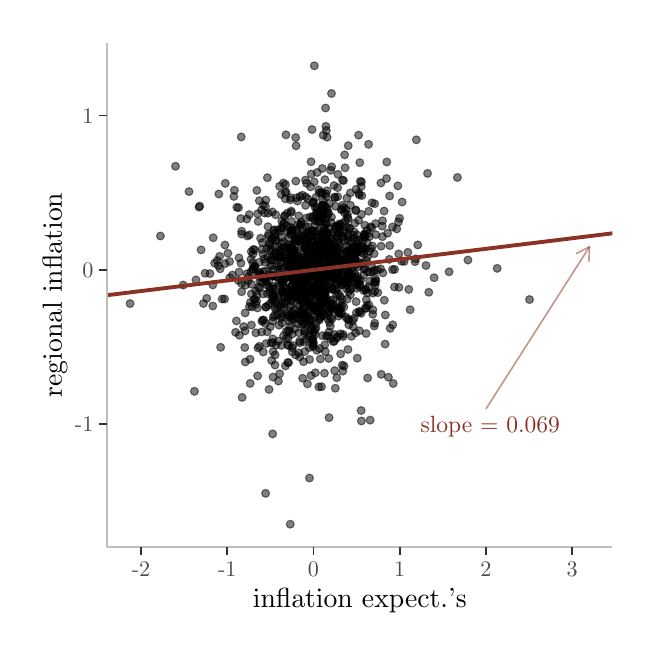
\begin{tikzpicture}[x=1pt,y=1pt]
\definecolor{fillColor}{RGB}{255,255,255}
\path[use as bounding box,fill=fillColor,fill opacity=0.00] (0,0) rectangle (216.81,216.81);
\begin{scope}
\path[clip] (  0.00,  0.00) rectangle (216.81,216.81);
\definecolor{drawColor}{RGB}{255,255,255}
\definecolor{fillColor}{RGB}{255,255,255}

\path[draw=drawColor,line width= 0.6pt,line join=round,line cap=round,fill=fillColor] (  0.00,  0.00) rectangle (216.81,216.81);
\end{scope}
\begin{scope}
\path[clip] ( 28.70, 29.10) rectangle (211.31,211.31);
\definecolor{drawColor}{RGB}{255,255,255}

\path[draw=drawColor,line width= 0.6pt,line join=round] ( 28.70, 73.48) --
	(211.31, 73.48);

\path[draw=drawColor,line width= 0.6pt,line join=round] ( 28.70,129.27) --
	(211.31,129.27);

\path[draw=drawColor,line width= 0.6pt,line join=round] ( 28.70,185.06) --
	(211.31,185.06);

\path[draw=drawColor,line width= 0.6pt,line join=round] ( 40.96, 29.10) --
	( 40.96,211.31);

\path[draw=drawColor,line width= 0.6pt,line join=round] ( 72.12, 29.10) --
	( 72.12,211.31);

\path[draw=drawColor,line width= 0.6pt,line join=round] (103.29, 29.10) --
	(103.29,211.31);

\path[draw=drawColor,line width= 0.6pt,line join=round] (134.45, 29.10) --
	(134.45,211.31);

\path[draw=drawColor,line width= 0.6pt,line join=round] (165.61, 29.10) --
	(165.61,211.31);

\path[draw=drawColor,line width= 0.6pt,line join=round] (196.78, 29.10) --
	(196.78,211.31);
\definecolor{drawColor}{RGB}{0,0,0}
\definecolor{fillColor}{RGB}{0,0,0}

\path[draw=drawColor,draw opacity=0.50,line width= 0.4pt,line join=round,line cap=round,fill=fillColor,fill opacity=0.50] (127.53,129.69) circle (  1.43);

\path[draw=drawColor,draw opacity=0.50,line width= 0.4pt,line join=round,line cap=round,fill=fillColor,fill opacity=0.50] (118.68,117.81) circle (  1.43);

\path[draw=drawColor,draw opacity=0.50,line width= 0.4pt,line join=round,line cap=round,fill=fillColor,fill opacity=0.50] (107.37,143.39) circle (  1.43);

\path[draw=drawColor,draw opacity=0.50,line width= 0.4pt,line join=round,line cap=round,fill=fillColor,fill opacity=0.50] (130.05,142.54) circle (  1.43);

\path[draw=drawColor,draw opacity=0.50,line width= 0.4pt,line join=round,line cap=round,fill=fillColor,fill opacity=0.50] ( 86.44,123.78) circle (  1.43);

\path[draw=drawColor,draw opacity=0.50,line width= 0.4pt,line join=round,line cap=round,fill=fillColor,fill opacity=0.50] (104.52,132.90) circle (  1.43);

\path[draw=drawColor,draw opacity=0.50,line width= 0.4pt,line join=round,line cap=round,fill=fillColor,fill opacity=0.50] (109.44,133.29) circle (  1.43);

\path[draw=drawColor,draw opacity=0.50,line width= 0.4pt,line join=round,line cap=round,fill=fillColor,fill opacity=0.50] (112.29,130.18) circle (  1.43);

\path[draw=drawColor,draw opacity=0.50,line width= 0.4pt,line join=round,line cap=round,fill=fillColor,fill opacity=0.50] ( 66.88,123.85) circle (  1.43);

\path[draw=drawColor,draw opacity=0.50,line width= 0.4pt,line join=round,line cap=round,fill=fillColor,fill opacity=0.50] (108.87,114.10) circle (  1.43);

\path[draw=drawColor,draw opacity=0.50,line width= 0.4pt,line join=round,line cap=round,fill=fillColor,fill opacity=0.50] ( 67.56,131.72) circle (  1.43);

\path[draw=drawColor,draw opacity=0.50,line width= 0.4pt,line join=round,line cap=round,fill=fillColor,fill opacity=0.50] ( 99.79,127.98) circle (  1.43);

\path[draw=drawColor,draw opacity=0.50,line width= 0.4pt,line join=round,line cap=round,fill=fillColor,fill opacity=0.50] (106.67,148.41) circle (  1.43);

\path[draw=drawColor,draw opacity=0.50,line width= 0.4pt,line join=round,line cap=round,fill=fillColor,fill opacity=0.50] (111.89,105.17) circle (  1.43);

\path[draw=drawColor,draw opacity=0.50,line width= 0.4pt,line join=round,line cap=round,fill=fillColor,fill opacity=0.50] (100.01,140.46) circle (  1.43);

\path[draw=drawColor,draw opacity=0.50,line width= 0.4pt,line join=round,line cap=round,fill=fillColor,fill opacity=0.50] (105.33,125.35) circle (  1.43);

\path[draw=drawColor,draw opacity=0.50,line width= 0.4pt,line join=round,line cap=round,fill=fillColor,fill opacity=0.50] (102.88,105.69) circle (  1.43);

\path[draw=drawColor,draw opacity=0.50,line width= 0.4pt,line join=round,line cap=round,fill=fillColor,fill opacity=0.50] (100.97,139.45) circle (  1.43);

\path[draw=drawColor,draw opacity=0.50,line width= 0.4pt,line join=round,line cap=round,fill=fillColor,fill opacity=0.50] ( 53.42,166.72) circle (  1.43);

\path[draw=drawColor,draw opacity=0.50,line width= 0.4pt,line join=round,line cap=round,fill=fillColor,fill opacity=0.50] (115.30,126.23) circle (  1.43);

\path[draw=drawColor,draw opacity=0.50,line width= 0.4pt,line join=round,line cap=round,fill=fillColor,fill opacity=0.50] (122.30,106.28) circle (  1.43);

\path[draw=drawColor,draw opacity=0.50,line width= 0.4pt,line join=round,line cap=round,fill=fillColor,fill opacity=0.50] (134.09,135.05) circle (  1.43);

\path[draw=drawColor,draw opacity=0.50,line width= 0.4pt,line join=round,line cap=round,fill=fillColor,fill opacity=0.50] (117.01,122.76) circle (  1.43);

\path[draw=drawColor,draw opacity=0.50,line width= 0.4pt,line join=round,line cap=round,fill=fillColor,fill opacity=0.50] ( 69.55,129.67) circle (  1.43);

\path[draw=drawColor,draw opacity=0.50,line width= 0.4pt,line join=round,line cap=round,fill=fillColor,fill opacity=0.50] (137.37,135.62) circle (  1.43);

\path[draw=drawColor,draw opacity=0.50,line width= 0.4pt,line join=round,line cap=round,fill=fillColor,fill opacity=0.50] ( 77.32,121.38) circle (  1.43);

\path[draw=drawColor,draw opacity=0.50,line width= 0.4pt,line join=round,line cap=round,fill=fillColor,fill opacity=0.50] (105.12,126.94) circle (  1.43);

\path[draw=drawColor,draw opacity=0.50,line width= 0.4pt,line join=round,line cap=round,fill=fillColor,fill opacity=0.50] (119.38,124.53) circle (  1.43);

\path[draw=drawColor,draw opacity=0.50,line width= 0.4pt,line join=round,line cap=round,fill=fillColor,fill opacity=0.50] ( 97.98,141.95) circle (  1.43);

\path[draw=drawColor,draw opacity=0.50,line width= 0.4pt,line join=round,line cap=round,fill=fillColor,fill opacity=0.50] ( 88.32,127.28) circle (  1.43);

\path[draw=drawColor,draw opacity=0.50,line width= 0.4pt,line join=round,line cap=round,fill=fillColor,fill opacity=0.50] (118.39,134.80) circle (  1.43);

\path[draw=drawColor,draw opacity=0.50,line width= 0.4pt,line join=round,line cap=round,fill=fillColor,fill opacity=0.50] ( 82.40,121.64) circle (  1.43);

\path[draw=drawColor,draw opacity=0.50,line width= 0.4pt,line join=round,line cap=round,fill=fillColor,fill opacity=0.50] ( 69.35,134.18) circle (  1.43);

\path[draw=drawColor,draw opacity=0.50,line width= 0.4pt,line join=round,line cap=round,fill=fillColor,fill opacity=0.50] ( 71.37,131.57) circle (  1.43);

\path[draw=drawColor,draw opacity=0.50,line width= 0.4pt,line join=round,line cap=round,fill=fillColor,fill opacity=0.50] ( 62.17,152.33) circle (  1.43);

\path[draw=drawColor,draw opacity=0.50,line width= 0.4pt,line join=round,line cap=round,fill=fillColor,fill opacity=0.50] ( 97.62,132.94) circle (  1.43);

\path[draw=drawColor,draw opacity=0.50,line width= 0.4pt,line join=round,line cap=round,fill=fillColor,fill opacity=0.50] ( 60.81,125.67) circle (  1.43);

\path[draw=drawColor,draw opacity=0.50,line width= 0.4pt,line join=round,line cap=round,fill=fillColor,fill opacity=0.50] (117.69,133.68) circle (  1.43);

\path[draw=drawColor,draw opacity=0.50,line width= 0.4pt,line join=round,line cap=round,fill=fillColor,fill opacity=0.50] (122.92,142.34) circle (  1.43);

\path[draw=drawColor,draw opacity=0.50,line width= 0.4pt,line join=round,line cap=round,fill=fillColor,fill opacity=0.50] (126.39,129.28) circle (  1.43);

\path[draw=drawColor,draw opacity=0.50,line width= 0.4pt,line join=round,line cap=round,fill=fillColor,fill opacity=0.50] ( 94.63,110.68) circle (  1.43);

\path[draw=drawColor,draw opacity=0.50,line width= 0.4pt,line join=round,line cap=round,fill=fillColor,fill opacity=0.50] (109.63,115.28) circle (  1.43);

\path[draw=drawColor,draw opacity=0.50,line width= 0.4pt,line join=round,line cap=round,fill=fillColor,fill opacity=0.50] (181.33,118.57) circle (  1.43);

\path[draw=drawColor,draw opacity=0.50,line width= 0.4pt,line join=round,line cap=round,fill=fillColor,fill opacity=0.50] (125.53,124.71) circle (  1.43);

\path[draw=drawColor,draw opacity=0.50,line width= 0.4pt,line join=round,line cap=round,fill=fillColor,fill opacity=0.50] (112.50,145.87) circle (  1.43);

\path[draw=drawColor,draw opacity=0.50,line width= 0.4pt,line join=round,line cap=round,fill=fillColor,fill opacity=0.50] ( 96.37,129.74) circle (  1.43);

\path[draw=drawColor,draw opacity=0.50,line width= 0.4pt,line join=round,line cap=round,fill=fillColor,fill opacity=0.50] ( 77.30,142.23) circle (  1.43);

\path[draw=drawColor,draw opacity=0.50,line width= 0.4pt,line join=round,line cap=round,fill=fillColor,fill opacity=0.50] ( 81.40,134.97) circle (  1.43);

\path[draw=drawColor,draw opacity=0.50,line width= 0.4pt,line join=round,line cap=round,fill=fillColor,fill opacity=0.50] ( 87.02,141.52) circle (  1.43);

\path[draw=drawColor,draw opacity=0.50,line width= 0.4pt,line join=round,line cap=round,fill=fillColor,fill opacity=0.50] (114.63,128.45) circle (  1.43);

\path[draw=drawColor,draw opacity=0.50,line width= 0.4pt,line join=round,line cap=round,fill=fillColor,fill opacity=0.50] ( 95.94,122.05) circle (  1.43);

\path[draw=drawColor,draw opacity=0.50,line width= 0.4pt,line join=round,line cap=round,fill=fillColor,fill opacity=0.50] (103.79,133.38) circle (  1.43);

\path[draw=drawColor,draw opacity=0.50,line width= 0.4pt,line join=round,line cap=round,fill=fillColor,fill opacity=0.50] (122.17,122.20) circle (  1.43);

\path[draw=drawColor,draw opacity=0.50,line width= 0.4pt,line join=round,line cap=round,fill=fillColor,fill opacity=0.50] (112.42,113.66) circle (  1.43);

\path[draw=drawColor,draw opacity=0.50,line width= 0.4pt,line join=round,line cap=round,fill=fillColor,fill opacity=0.50] (120.36,125.64) circle (  1.43);

\path[draw=drawColor,draw opacity=0.50,line width= 0.4pt,line join=round,line cap=round,fill=fillColor,fill opacity=0.50] (115.53,111.50) circle (  1.43);

\path[draw=drawColor,draw opacity=0.50,line width= 0.4pt,line join=round,line cap=round,fill=fillColor,fill opacity=0.50] (118.12,134.10) circle (  1.43);

\path[draw=drawColor,draw opacity=0.50,line width= 0.4pt,line join=round,line cap=round,fill=fillColor,fill opacity=0.50] (107.63,119.91) circle (  1.43);

\path[draw=drawColor,draw opacity=0.50,line width= 0.4pt,line join=round,line cap=round,fill=fillColor,fill opacity=0.50] ( 74.00,127.41) circle (  1.43);

\path[draw=drawColor,draw opacity=0.50,line width= 0.4pt,line join=round,line cap=round,fill=fillColor,fill opacity=0.50] (101.23,136.38) circle (  1.43);

\path[draw=drawColor,draw opacity=0.50,line width= 0.4pt,line join=round,line cap=round,fill=fillColor,fill opacity=0.50] ( 56.21,123.80) circle (  1.43);

\path[draw=drawColor,draw opacity=0.50,line width= 0.4pt,line join=round,line cap=round,fill=fillColor,fill opacity=0.50] (146.86,126.47) circle (  1.43);

\path[draw=drawColor,draw opacity=0.50,line width= 0.4pt,line join=round,line cap=round,fill=fillColor,fill opacity=0.50] (104.79,114.86) circle (  1.43);

\path[draw=drawColor,draw opacity=0.50,line width= 0.4pt,line join=round,line cap=round,fill=fillColor,fill opacity=0.50] (119.63,157.02) circle (  1.43);

\path[draw=drawColor,draw opacity=0.50,line width= 0.4pt,line join=round,line cap=round,fill=fillColor,fill opacity=0.50] ( 73.03,126.43) circle (  1.43);

\path[draw=drawColor,draw opacity=0.50,line width= 0.4pt,line join=round,line cap=round,fill=fillColor,fill opacity=0.50] ( 96.69,132.21) circle (  1.43);

\path[draw=drawColor,draw opacity=0.50,line width= 0.4pt,line join=round,line cap=round,fill=fillColor,fill opacity=0.50] (105.22,120.31) circle (  1.43);

\path[draw=drawColor,draw opacity=0.50,line width= 0.4pt,line join=round,line cap=round,fill=fillColor,fill opacity=0.50] (136.02,132.33) circle (  1.43);

\path[draw=drawColor,draw opacity=0.50,line width= 0.4pt,line join=round,line cap=round,fill=fillColor,fill opacity=0.50] (115.08,112.19) circle (  1.43);

\path[draw=drawColor,draw opacity=0.50,line width= 0.4pt,line join=round,line cap=round,fill=fillColor,fill opacity=0.50] (120.95,136.25) circle (  1.43);

\path[draw=drawColor,draw opacity=0.50,line width= 0.4pt,line join=round,line cap=round,fill=fillColor,fill opacity=0.50] ( 76.36,133.61) circle (  1.43);

\path[draw=drawColor,draw opacity=0.50,line width= 0.4pt,line join=round,line cap=round,fill=fillColor,fill opacity=0.50] (100.75,135.02) circle (  1.43);

\path[draw=drawColor,draw opacity=0.50,line width= 0.4pt,line join=round,line cap=round,fill=fillColor,fill opacity=0.50] ( 88.89,143.45) circle (  1.43);

\path[draw=drawColor,draw opacity=0.50,line width= 0.4pt,line join=round,line cap=round,fill=fillColor,fill opacity=0.50] (120.02,123.95) circle (  1.43);

\path[draw=drawColor,draw opacity=0.50,line width= 0.4pt,line join=round,line cap=round,fill=fillColor,fill opacity=0.50] ( 98.68,118.70) circle (  1.43);

\path[draw=drawColor,draw opacity=0.50,line width= 0.4pt,line join=round,line cap=round,fill=fillColor,fill opacity=0.50] (105.56,130.97) circle (  1.43);

\path[draw=drawColor,draw opacity=0.50,line width= 0.4pt,line join=round,line cap=round,fill=fillColor,fill opacity=0.50] (117.42,110.95) circle (  1.43);

\path[draw=drawColor,draw opacity=0.50,line width= 0.4pt,line join=round,line cap=round,fill=fillColor,fill opacity=0.50] (125.42,129.16) circle (  1.43);

\path[draw=drawColor,draw opacity=0.50,line width= 0.4pt,line join=round,line cap=round,fill=fillColor,fill opacity=0.50] ( 87.63,138.24) circle (  1.43);

\path[draw=drawColor,draw opacity=0.50,line width= 0.4pt,line join=round,line cap=round,fill=fillColor,fill opacity=0.50] (125.86,125.42) circle (  1.43);

\path[draw=drawColor,draw opacity=0.50,line width= 0.4pt,line join=round,line cap=round,fill=fillColor,fill opacity=0.50] (131.92,109.44) circle (  1.43);

\path[draw=drawColor,draw opacity=0.50,line width= 0.4pt,line join=round,line cap=round,fill=fillColor,fill opacity=0.50] ( 92.95,126.84) circle (  1.43);

\path[draw=drawColor,draw opacity=0.50,line width= 0.4pt,line join=round,line cap=round,fill=fillColor,fill opacity=0.50] ( 80.68,128.50) circle (  1.43);

\path[draw=drawColor,draw opacity=0.50,line width= 0.4pt,line join=round,line cap=round,fill=fillColor,fill opacity=0.50] ( 94.44,131.34) circle (  1.43);

\path[draw=drawColor,draw opacity=0.50,line width= 0.4pt,line join=round,line cap=round,fill=fillColor,fill opacity=0.50] ( 98.85,130.18) circle (  1.43);

\path[draw=drawColor,draw opacity=0.50,line width= 0.4pt,line join=round,line cap=round,fill=fillColor,fill opacity=0.50] (100.53,144.91) circle (  1.43);

\path[draw=drawColor,draw opacity=0.50,line width= 0.4pt,line join=round,line cap=round,fill=fillColor,fill opacity=0.50] ( 89.38,135.35) circle (  1.43);

\path[draw=drawColor,draw opacity=0.50,line width= 0.4pt,line join=round,line cap=round,fill=fillColor,fill opacity=0.50] ( 94.36,140.88) circle (  1.43);

\path[draw=drawColor,draw opacity=0.50,line width= 0.4pt,line join=round,line cap=round,fill=fillColor,fill opacity=0.50] (104.06,132.28) circle (  1.43);

\path[draw=drawColor,draw opacity=0.50,line width= 0.4pt,line join=round,line cap=round,fill=fillColor,fill opacity=0.50] ( 86.08,128.75) circle (  1.43);

\path[draw=drawColor,draw opacity=0.50,line width= 0.4pt,line join=round,line cap=round,fill=fillColor,fill opacity=0.50] (115.91,127.88) circle (  1.43);

\path[draw=drawColor,draw opacity=0.50,line width= 0.4pt,line join=round,line cap=round,fill=fillColor,fill opacity=0.50] ( 64.11,128.06) circle (  1.43);

\path[draw=drawColor,draw opacity=0.50,line width= 0.4pt,line join=round,line cap=round,fill=fillColor,fill opacity=0.50] (114.73,133.45) circle (  1.43);

\path[draw=drawColor,draw opacity=0.50,line width= 0.4pt,line join=round,line cap=round,fill=fillColor,fill opacity=0.50] (100.92,143.12) circle (  1.43);

\path[draw=drawColor,draw opacity=0.50,line width= 0.4pt,line join=round,line cap=round,fill=fillColor,fill opacity=0.50] ( 94.60,136.81) circle (  1.43);

\path[draw=drawColor,draw opacity=0.50,line width= 0.4pt,line join=round,line cap=round,fill=fillColor,fill opacity=0.50] (110.31,118.54) circle (  1.43);

\path[draw=drawColor,draw opacity=0.50,line width= 0.4pt,line join=round,line cap=round,fill=fillColor,fill opacity=0.50] (115.14,122.58) circle (  1.43);

\path[draw=drawColor,draw opacity=0.50,line width= 0.4pt,line join=round,line cap=round,fill=fillColor,fill opacity=0.50] (112.37,120.66) circle (  1.43);

\path[draw=drawColor,draw opacity=0.50,line width= 0.4pt,line join=round,line cap=round,fill=fillColor,fill opacity=0.50] (111.23,126.10) circle (  1.43);

\path[draw=drawColor,draw opacity=0.50,line width= 0.4pt,line join=round,line cap=round,fill=fillColor,fill opacity=0.50] (109.96,132.99) circle (  1.43);

\path[draw=drawColor,draw opacity=0.50,line width= 0.4pt,line join=round,line cap=round,fill=fillColor,fill opacity=0.50] ( 97.72,128.89) circle (  1.43);

\path[draw=drawColor,draw opacity=0.50,line width= 0.4pt,line join=round,line cap=round,fill=fillColor,fill opacity=0.50] ( 86.58,106.89) circle (  1.43);

\path[draw=drawColor,draw opacity=0.50,line width= 0.4pt,line join=round,line cap=round,fill=fillColor,fill opacity=0.50] ( 87.25,123.16) circle (  1.43);

\path[draw=drawColor,draw opacity=0.50,line width= 0.4pt,line join=round,line cap=round,fill=fillColor,fill opacity=0.50] ( 99.67,117.62) circle (  1.43);

\path[draw=drawColor,draw opacity=0.50,line width= 0.4pt,line join=round,line cap=round,fill=fillColor,fill opacity=0.50] (122.77,120.95) circle (  1.43);

\path[draw=drawColor,draw opacity=0.50,line width= 0.4pt,line join=round,line cap=round,fill=fillColor,fill opacity=0.50] (108.18,157.89) circle (  1.43);

\path[draw=drawColor,draw opacity=0.50,line width= 0.4pt,line join=round,line cap=round,fill=fillColor,fill opacity=0.50] (114.60,139.57) circle (  1.43);

\path[draw=drawColor,draw opacity=0.50,line width= 0.4pt,line join=round,line cap=round,fill=fillColor,fill opacity=0.50] (121.80,136.78) circle (  1.43);

\path[draw=drawColor,draw opacity=0.50,line width= 0.4pt,line join=round,line cap=round,fill=fillColor,fill opacity=0.50] (115.99,121.45) circle (  1.43);

\path[draw=drawColor,draw opacity=0.50,line width= 0.4pt,line join=round,line cap=round,fill=fillColor,fill opacity=0.50] ( 87.85,136.93) circle (  1.43);

\path[draw=drawColor,draw opacity=0.50,line width= 0.4pt,line join=round,line cap=round,fill=fillColor,fill opacity=0.50] (109.87,122.25) circle (  1.43);

\path[draw=drawColor,draw opacity=0.50,line width= 0.4pt,line join=round,line cap=round,fill=fillColor,fill opacity=0.50] ( 87.16,138.84) circle (  1.43);

\path[draw=drawColor,draw opacity=0.50,line width= 0.4pt,line join=round,line cap=round,fill=fillColor,fill opacity=0.50] (100.95,140.89) circle (  1.43);

\path[draw=drawColor,draw opacity=0.50,line width= 0.4pt,line join=round,line cap=round,fill=fillColor,fill opacity=0.50] (103.86,133.96) circle (  1.43);

\path[draw=drawColor,draw opacity=0.50,line width= 0.4pt,line join=round,line cap=round,fill=fillColor,fill opacity=0.50] (117.75,134.27) circle (  1.43);

\path[draw=drawColor,draw opacity=0.50,line width= 0.4pt,line join=round,line cap=round,fill=fillColor,fill opacity=0.50] ( 85.49,133.25) circle (  1.43);

\path[draw=drawColor,draw opacity=0.50,line width= 0.4pt,line join=round,line cap=round,fill=fillColor,fill opacity=0.50] ( 94.45,130.58) circle (  1.43);

\path[draw=drawColor,draw opacity=0.50,line width= 0.4pt,line join=round,line cap=round,fill=fillColor,fill opacity=0.50] ( 81.32,129.48) circle (  1.43);

\path[draw=drawColor,draw opacity=0.50,line width= 0.4pt,line join=round,line cap=round,fill=fillColor,fill opacity=0.50] (106.97,113.09) circle (  1.43);

\path[draw=drawColor,draw opacity=0.50,line width= 0.4pt,line join=round,line cap=round,fill=fillColor,fill opacity=0.50] (128.20,141.29) circle (  1.43);

\path[draw=drawColor,draw opacity=0.50,line width= 0.4pt,line join=round,line cap=round,fill=fillColor,fill opacity=0.50] ( 90.24,112.97) circle (  1.43);

\path[draw=drawColor,draw opacity=0.50,line width= 0.4pt,line join=round,line cap=round,fill=fillColor,fill opacity=0.50] (109.20,130.99) circle (  1.43);

\path[draw=drawColor,draw opacity=0.50,line width= 0.4pt,line join=round,line cap=round,fill=fillColor,fill opacity=0.50] ( 99.56,120.90) circle (  1.43);

\path[draw=drawColor,draw opacity=0.50,line width= 0.4pt,line join=round,line cap=round,fill=fillColor,fill opacity=0.50] (121.43,129.56) circle (  1.43);

\path[draw=drawColor,draw opacity=0.50,line width= 0.4pt,line join=round,line cap=round,fill=fillColor,fill opacity=0.50] (115.72,141.64) circle (  1.43);

\path[draw=drawColor,draw opacity=0.50,line width= 0.4pt,line join=round,line cap=round,fill=fillColor,fill opacity=0.50] (100.70,148.01) circle (  1.43);

\path[draw=drawColor,draw opacity=0.50,line width= 0.4pt,line join=round,line cap=round,fill=fillColor,fill opacity=0.50] (114.74,127.27) circle (  1.43);

\path[draw=drawColor,draw opacity=0.50,line width= 0.4pt,line join=round,line cap=round,fill=fillColor,fill opacity=0.50] (109.59,136.12) circle (  1.43);

\path[draw=drawColor,draw opacity=0.50,line width= 0.4pt,line join=round,line cap=round,fill=fillColor,fill opacity=0.50] (112.29,136.62) circle (  1.43);

\path[draw=drawColor,draw opacity=0.50,line width= 0.4pt,line join=round,line cap=round,fill=fillColor,fill opacity=0.50] (121.43,121.79) circle (  1.43);

\path[draw=drawColor,draw opacity=0.50,line width= 0.4pt,line join=round,line cap=round,fill=fillColor,fill opacity=0.50] (115.89,132.81) circle (  1.43);

\path[draw=drawColor,draw opacity=0.50,line width= 0.4pt,line join=round,line cap=round,fill=fillColor,fill opacity=0.50] ( 97.91,123.86) circle (  1.43);

\path[draw=drawColor,draw opacity=0.50,line width= 0.4pt,line join=round,line cap=round,fill=fillColor,fill opacity=0.50] ( 80.86,124.10) circle (  1.43);

\path[draw=drawColor,draw opacity=0.50,line width= 0.4pt,line join=round,line cap=round,fill=fillColor,fill opacity=0.50] ( 88.97,118.50) circle (  1.43);

\path[draw=drawColor,draw opacity=0.50,line width= 0.4pt,line join=round,line cap=round,fill=fillColor,fill opacity=0.50] ( 66.89,116.24) circle (  1.43);

\path[draw=drawColor,draw opacity=0.50,line width= 0.4pt,line join=round,line cap=round,fill=fillColor,fill opacity=0.50] (114.44,124.27) circle (  1.43);

\path[draw=drawColor,draw opacity=0.50,line width= 0.4pt,line join=round,line cap=round,fill=fillColor,fill opacity=0.50] ( 91.46,115.93) circle (  1.43);

\path[draw=drawColor,draw opacity=0.50,line width= 0.4pt,line join=round,line cap=round,fill=fillColor,fill opacity=0.50] ( 93.35,132.33) circle (  1.43);

\path[draw=drawColor,draw opacity=0.50,line width= 0.4pt,line join=round,line cap=round,fill=fillColor,fill opacity=0.50] (106.18,135.78) circle (  1.43);

\path[draw=drawColor,draw opacity=0.50,line width= 0.4pt,line join=round,line cap=round,fill=fillColor,fill opacity=0.50] (117.56,137.33) circle (  1.43);

\path[draw=drawColor,draw opacity=0.50,line width= 0.4pt,line join=round,line cap=round,fill=fillColor,fill opacity=0.50] (115.81,124.46) circle (  1.43);

\path[draw=drawColor,draw opacity=0.50,line width= 0.4pt,line join=round,line cap=round,fill=fillColor,fill opacity=0.50] ( 91.62,111.85) circle (  1.43);

\path[draw=drawColor,draw opacity=0.50,line width= 0.4pt,line join=round,line cap=round,fill=fillColor,fill opacity=0.50] (119.68,130.54) circle (  1.43);

\path[draw=drawColor,draw opacity=0.50,line width= 0.4pt,line join=round,line cap=round,fill=fillColor,fill opacity=0.50] ( 87.84,136.09) circle (  1.43);

\path[draw=drawColor,draw opacity=0.50,line width= 0.4pt,line join=round,line cap=round,fill=fillColor,fill opacity=0.50] (106.70,129.45) circle (  1.43);

\path[draw=drawColor,draw opacity=0.50,line width= 0.4pt,line join=round,line cap=round,fill=fillColor,fill opacity=0.50] ( 91.60,135.85) circle (  1.43);

\path[draw=drawColor,draw opacity=0.50,line width= 0.4pt,line join=round,line cap=round,fill=fillColor,fill opacity=0.50] (101.57,134.11) circle (  1.43);

\path[draw=drawColor,draw opacity=0.50,line width= 0.4pt,line join=round,line cap=round,fill=fillColor,fill opacity=0.50] (116.06,127.49) circle (  1.43);

\path[draw=drawColor,draw opacity=0.50,line width= 0.4pt,line join=round,line cap=round,fill=fillColor,fill opacity=0.50] ( 99.67,128.59) circle (  1.43);

\path[draw=drawColor,draw opacity=0.50,line width= 0.4pt,line join=round,line cap=round,fill=fillColor,fill opacity=0.50] (113.04,145.64) circle (  1.43);

\path[draw=drawColor,draw opacity=0.50,line width= 0.4pt,line join=round,line cap=round,fill=fillColor,fill opacity=0.50] ( 83.84,128.06) circle (  1.43);

\path[draw=drawColor,draw opacity=0.50,line width= 0.4pt,line join=round,line cap=round,fill=fillColor,fill opacity=0.50] (128.80,150.55) circle (  1.43);

\path[draw=drawColor,draw opacity=0.50,line width= 0.4pt,line join=round,line cap=round,fill=fillColor,fill opacity=0.50] ( 99.16,113.02) circle (  1.43);

\path[draw=drawColor,draw opacity=0.50,line width= 0.4pt,line join=round,line cap=round,fill=fillColor,fill opacity=0.50] ( 95.46,111.74) circle (  1.43);

\path[draw=drawColor,draw opacity=0.50,line width= 0.4pt,line join=round,line cap=round,fill=fillColor,fill opacity=0.50] (116.36,124.51) circle (  1.43);

\path[draw=drawColor,draw opacity=0.50,line width= 0.4pt,line join=round,line cap=round,fill=fillColor,fill opacity=0.50] (100.19,121.85) circle (  1.43);

\path[draw=drawColor,draw opacity=0.50,line width= 0.4pt,line join=round,line cap=round,fill=fillColor,fill opacity=0.50] (111.63,120.30) circle (  1.43);

\path[draw=drawColor,draw opacity=0.50,line width= 0.4pt,line join=round,line cap=round,fill=fillColor,fill opacity=0.50] (110.25,134.68) circle (  1.43);

\path[draw=drawColor,draw opacity=0.50,line width= 0.4pt,line join=round,line cap=round,fill=fillColor,fill opacity=0.50] ( 89.72,140.38) circle (  1.43);

\path[draw=drawColor,draw opacity=0.50,line width= 0.4pt,line join=round,line cap=round,fill=fillColor,fill opacity=0.50] ( 91.32,131.91) circle (  1.43);

\path[draw=drawColor,draw opacity=0.50,line width= 0.4pt,line join=round,line cap=round,fill=fillColor,fill opacity=0.50] (116.94,126.84) circle (  1.43);

\path[draw=drawColor,draw opacity=0.50,line width= 0.4pt,line join=round,line cap=round,fill=fillColor,fill opacity=0.50] ( 89.44,137.64) circle (  1.43);

\path[draw=drawColor,draw opacity=0.50,line width= 0.4pt,line join=round,line cap=round,fill=fillColor,fill opacity=0.50] ( 85.83,132.04) circle (  1.43);

\path[draw=drawColor,draw opacity=0.50,line width= 0.4pt,line join=round,line cap=round,fill=fillColor,fill opacity=0.50] (114.93,133.32) circle (  1.43);

\path[draw=drawColor,draw opacity=0.50,line width= 0.4pt,line join=round,line cap=round,fill=fillColor,fill opacity=0.50] ( 78.59,113.72) circle (  1.43);

\path[draw=drawColor,draw opacity=0.50,line width= 0.4pt,line join=round,line cap=round,fill=fillColor,fill opacity=0.50] ( 94.71,120.50) circle (  1.43);

\path[draw=drawColor,draw opacity=0.50,line width= 0.4pt,line join=round,line cap=round,fill=fillColor,fill opacity=0.50] (110.73,135.84) circle (  1.43);

\path[draw=drawColor,draw opacity=0.50,line width= 0.4pt,line join=round,line cap=round,fill=fillColor,fill opacity=0.50] ( 99.52,115.59) circle (  1.43);

\path[draw=drawColor,draw opacity=0.50,line width= 0.4pt,line join=round,line cap=round,fill=fillColor,fill opacity=0.50] (143.93,130.86) circle (  1.43);

\path[draw=drawColor,draw opacity=0.50,line width= 0.4pt,line join=round,line cap=round,fill=fillColor,fill opacity=0.50] ( 89.80,135.52) circle (  1.43);

\path[draw=drawColor,draw opacity=0.50,line width= 0.4pt,line join=round,line cap=round,fill=fillColor,fill opacity=0.50] (115.43,134.47) circle (  1.43);

\path[draw=drawColor,draw opacity=0.50,line width= 0.4pt,line join=round,line cap=round,fill=fillColor,fill opacity=0.50] ( 99.57,134.88) circle (  1.43);

\path[draw=drawColor,draw opacity=0.50,line width= 0.4pt,line join=round,line cap=round,fill=fillColor,fill opacity=0.50] ( 95.30,134.93) circle (  1.43);

\path[draw=drawColor,draw opacity=0.50,line width= 0.4pt,line join=round,line cap=round,fill=fillColor,fill opacity=0.50] (104.23,118.66) circle (  1.43);

\path[draw=drawColor,draw opacity=0.50,line width= 0.4pt,line join=round,line cap=round,fill=fillColor,fill opacity=0.50] ( 85.92,125.60) circle (  1.43);

\path[draw=drawColor,draw opacity=0.50,line width= 0.4pt,line join=round,line cap=round,fill=fillColor,fill opacity=0.50] (125.73,146.01) circle (  1.43);

\path[draw=drawColor,draw opacity=0.50,line width= 0.4pt,line join=round,line cap=round,fill=fillColor,fill opacity=0.50] (169.65,129.84) circle (  1.43);

\path[draw=drawColor,draw opacity=0.50,line width= 0.4pt,line join=round,line cap=round,fill=fillColor,fill opacity=0.50] (109.99,134.74) circle (  1.43);

\path[draw=drawColor,draw opacity=0.50,line width= 0.4pt,line join=round,line cap=round,fill=fillColor,fill opacity=0.50] ( 99.38,128.79) circle (  1.43);

\path[draw=drawColor,draw opacity=0.50,line width= 0.4pt,line join=round,line cap=round,fill=fillColor,fill opacity=0.50] (114.86,129.21) circle (  1.43);

\path[draw=drawColor,draw opacity=0.50,line width= 0.4pt,line join=round,line cap=round,fill=fillColor,fill opacity=0.50] ( 37.00,117.10) circle (  1.43);

\path[draw=drawColor,draw opacity=0.50,line width= 0.4pt,line join=round,line cap=round,fill=fillColor,fill opacity=0.50] (101.77,121.61) circle (  1.43);

\path[draw=drawColor,draw opacity=0.50,line width= 0.4pt,line join=round,line cap=round,fill=fillColor,fill opacity=0.50] ( 81.83,118.59) circle (  1.43);

\path[draw=drawColor,draw opacity=0.50,line width= 0.4pt,line join=round,line cap=round,fill=fillColor,fill opacity=0.50] (113.78,146.14) circle (  1.43);

\path[draw=drawColor,draw opacity=0.50,line width= 0.4pt,line join=round,line cap=round,fill=fillColor,fill opacity=0.50] (104.76,141.99) circle (  1.43);

\path[draw=drawColor,draw opacity=0.50,line width= 0.4pt,line join=round,line cap=round,fill=fillColor,fill opacity=0.50] ( 94.42,132.97) circle (  1.43);

\path[draw=drawColor,draw opacity=0.50,line width= 0.4pt,line join=round,line cap=round,fill=fillColor,fill opacity=0.50] ( 96.85,121.09) circle (  1.43);

\path[draw=drawColor,draw opacity=0.50,line width= 0.4pt,line join=round,line cap=round,fill=fillColor,fill opacity=0.50] (110.92,128.99) circle (  1.43);

\path[draw=drawColor,draw opacity=0.50,line width= 0.4pt,line join=round,line cap=round,fill=fillColor,fill opacity=0.50] ( 99.54,122.61) circle (  1.43);

\path[draw=drawColor,draw opacity=0.50,line width= 0.4pt,line join=round,line cap=round,fill=fillColor,fill opacity=0.50] ( 92.72,133.81) circle (  1.43);

\path[draw=drawColor,draw opacity=0.50,line width= 0.4pt,line join=round,line cap=round,fill=fillColor,fill opacity=0.50] (105.99,128.20) circle (  1.43);

\path[draw=drawColor,draw opacity=0.50,line width= 0.4pt,line join=round,line cap=round,fill=fillColor,fill opacity=0.50] (112.37,114.82) circle (  1.43);

\path[draw=drawColor,draw opacity=0.50,line width= 0.4pt,line join=round,line cap=round,fill=fillColor,fill opacity=0.50] (118.67,131.28) circle (  1.43);

\path[draw=drawColor,draw opacity=0.50,line width= 0.4pt,line join=round,line cap=round,fill=fillColor,fill opacity=0.50] ( 91.77,125.28) circle (  1.43);

\path[draw=drawColor,draw opacity=0.50,line width= 0.4pt,line join=round,line cap=round,fill=fillColor,fill opacity=0.50] ( 90.19,132.59) circle (  1.43);

\path[draw=drawColor,draw opacity=0.50,line width= 0.4pt,line join=round,line cap=round,fill=fillColor,fill opacity=0.50] (121.23,137.60) circle (  1.43);

\path[draw=drawColor,draw opacity=0.50,line width= 0.4pt,line join=round,line cap=round,fill=fillColor,fill opacity=0.50] (122.55,116.29) circle (  1.43);

\path[draw=drawColor,draw opacity=0.50,line width= 0.4pt,line join=round,line cap=round,fill=fillColor,fill opacity=0.50] (106.52,129.11) circle (  1.43);

\path[draw=drawColor,draw opacity=0.50,line width= 0.4pt,line join=round,line cap=round,fill=fillColor,fill opacity=0.50] ( 83.65,127.58) circle (  1.43);

\path[draw=drawColor,draw opacity=0.50,line width= 0.4pt,line join=round,line cap=round,fill=fillColor,fill opacity=0.50] (124.76,114.84) circle (  1.43);

\path[draw=drawColor,draw opacity=0.50,line width= 0.4pt,line join=round,line cap=round,fill=fillColor,fill opacity=0.50] (112.67,138.33) circle (  1.43);

\path[draw=drawColor,draw opacity=0.50,line width= 0.4pt,line join=round,line cap=round,fill=fillColor,fill opacity=0.50] (118.52,150.75) circle (  1.43);

\path[draw=drawColor,draw opacity=0.50,line width= 0.4pt,line join=round,line cap=round,fill=fillColor,fill opacity=0.50] ( 76.37,128.49) circle (  1.43);

\path[draw=drawColor,draw opacity=0.50,line width= 0.4pt,line join=round,line cap=round,fill=fillColor,fill opacity=0.50] (104.83,133.65) circle (  1.43);

\path[draw=drawColor,draw opacity=0.50,line width= 0.4pt,line join=round,line cap=round,fill=fillColor,fill opacity=0.50] ( 95.68,114.02) circle (  1.43);

\path[draw=drawColor,draw opacity=0.50,line width= 0.4pt,line join=round,line cap=round,fill=fillColor,fill opacity=0.50] ( 94.99,138.07) circle (  1.43);

\path[draw=drawColor,draw opacity=0.50,line width= 0.4pt,line join=round,line cap=round,fill=fillColor,fill opacity=0.50] ( 88.18,133.99) circle (  1.43);

\path[draw=drawColor,draw opacity=0.50,line width= 0.4pt,line join=round,line cap=round,fill=fillColor,fill opacity=0.50] (110.72,126.12) circle (  1.43);

\path[draw=drawColor,draw opacity=0.50,line width= 0.4pt,line join=round,line cap=round,fill=fillColor,fill opacity=0.50] (110.48,133.66) circle (  1.43);

\path[draw=drawColor,draw opacity=0.50,line width= 0.4pt,line join=round,line cap=round,fill=fillColor,fill opacity=0.50] (118.23,132.03) circle (  1.43);

\path[draw=drawColor,draw opacity=0.50,line width= 0.4pt,line join=round,line cap=round,fill=fillColor,fill opacity=0.50] (128.36,128.20) circle (  1.43);

\path[draw=drawColor,draw opacity=0.50,line width= 0.4pt,line join=round,line cap=round,fill=fillColor,fill opacity=0.50] (103.73,131.46) circle (  1.43);

\path[draw=drawColor,draw opacity=0.50,line width= 0.4pt,line join=round,line cap=round,fill=fillColor,fill opacity=0.50] (104.71,131.30) circle (  1.43);

\path[draw=drawColor,draw opacity=0.50,line width= 0.4pt,line join=round,line cap=round,fill=fillColor,fill opacity=0.50] (115.22,135.53) circle (  1.43);

\path[draw=drawColor,draw opacity=0.50,line width= 0.4pt,line join=round,line cap=round,fill=fillColor,fill opacity=0.50] ( 77.09,131.70) circle (  1.43);

\path[draw=drawColor,draw opacity=0.50,line width= 0.4pt,line join=round,line cap=round,fill=fillColor,fill opacity=0.50] (107.34,140.86) circle (  1.43);

\path[draw=drawColor,draw opacity=0.50,line width= 0.4pt,line join=round,line cap=round,fill=fillColor,fill opacity=0.50] ( 93.18,133.39) circle (  1.43);

\path[draw=drawColor,draw opacity=0.50,line width= 0.4pt,line join=round,line cap=round,fill=fillColor,fill opacity=0.50] ( 88.54,104.35) circle (  1.43);

\path[draw=drawColor,draw opacity=0.50,line width= 0.4pt,line join=round,line cap=round,fill=fillColor,fill opacity=0.50] (103.19,133.34) circle (  1.43);

\path[draw=drawColor,draw opacity=0.50,line width= 0.4pt,line join=round,line cap=round,fill=fillColor,fill opacity=0.50] ( 89.36,115.39) circle (  1.43);

\path[draw=drawColor,draw opacity=0.50,line width= 0.4pt,line join=round,line cap=round,fill=fillColor,fill opacity=0.50] (107.77,128.69) circle (  1.43);

\path[draw=drawColor,draw opacity=0.50,line width= 0.4pt,line join=round,line cap=round,fill=fillColor,fill opacity=0.50] (100.54,128.09) circle (  1.43);

\path[draw=drawColor,draw opacity=0.50,line width= 0.4pt,line join=round,line cap=round,fill=fillColor,fill opacity=0.50] ( 90.81,133.88) circle (  1.43);

\path[draw=drawColor,draw opacity=0.50,line width= 0.4pt,line join=round,line cap=round,fill=fillColor,fill opacity=0.50] ( 97.48,126.13) circle (  1.43);

\path[draw=drawColor,draw opacity=0.50,line width= 0.4pt,line join=round,line cap=round,fill=fillColor,fill opacity=0.50] (108.63,123.01) circle (  1.43);

\path[draw=drawColor,draw opacity=0.50,line width= 0.4pt,line join=round,line cap=round,fill=fillColor,fill opacity=0.50] (107.97,127.79) circle (  1.43);

\path[draw=drawColor,draw opacity=0.50,line width= 0.4pt,line join=round,line cap=round,fill=fillColor,fill opacity=0.50] (100.43,125.65) circle (  1.43);

\path[draw=drawColor,draw opacity=0.50,line width= 0.4pt,line join=round,line cap=round,fill=fillColor,fill opacity=0.50] (123.16,123.21) circle (  1.43);

\path[draw=drawColor,draw opacity=0.50,line width= 0.4pt,line join=round,line cap=round,fill=fillColor,fill opacity=0.50] (110.17,130.65) circle (  1.43);

\path[draw=drawColor,draw opacity=0.50,line width= 0.4pt,line join=round,line cap=round,fill=fillColor,fill opacity=0.50] (102.76,139.12) circle (  1.43);

\path[draw=drawColor,draw opacity=0.50,line width= 0.4pt,line join=round,line cap=round,fill=fillColor,fill opacity=0.50] ( 84.16,140.74) circle (  1.43);

\path[draw=drawColor,draw opacity=0.50,line width= 0.4pt,line join=round,line cap=round,fill=fillColor,fill opacity=0.50] (105.55,124.26) circle (  1.43);

\path[draw=drawColor,draw opacity=0.50,line width= 0.4pt,line join=round,line cap=round,fill=fillColor,fill opacity=0.50] (121.92,115.39) circle (  1.43);

\path[draw=drawColor,draw opacity=0.50,line width= 0.4pt,line join=round,line cap=round,fill=fillColor,fill opacity=0.50] ( 75.42,110.84) circle (  1.43);

\path[draw=drawColor,draw opacity=0.50,line width= 0.4pt,line join=round,line cap=round,fill=fillColor,fill opacity=0.50] (106.12,146.86) circle (  1.43);

\path[draw=drawColor,draw opacity=0.50,line width= 0.4pt,line join=round,line cap=round,fill=fillColor,fill opacity=0.50] ( 89.85,126.87) circle (  1.43);

\path[draw=drawColor,draw opacity=0.50,line width= 0.4pt,line join=round,line cap=round,fill=fillColor,fill opacity=0.50] ( 96.26,136.33) circle (  1.43);

\path[draw=drawColor,draw opacity=0.50,line width= 0.4pt,line join=round,line cap=round,fill=fillColor,fill opacity=0.50] (117.99,142.99) circle (  1.43);

\path[draw=drawColor,draw opacity=0.50,line width= 0.4pt,line join=round,line cap=round,fill=fillColor,fill opacity=0.50] (114.83,125.76) circle (  1.43);

\path[draw=drawColor,draw opacity=0.50,line width= 0.4pt,line join=round,line cap=round,fill=fillColor,fill opacity=0.50] ( 85.21,126.58) circle (  1.43);

\path[draw=drawColor,draw opacity=0.50,line width= 0.4pt,line join=round,line cap=round,fill=fillColor,fill opacity=0.50] (101.59,128.51) circle (  1.43);

\path[draw=drawColor,draw opacity=0.50,line width= 0.4pt,line join=round,line cap=round,fill=fillColor,fill opacity=0.50] (110.00,122.70) circle (  1.43);

\path[draw=drawColor,draw opacity=0.50,line width= 0.4pt,line join=round,line cap=round,fill=fillColor,fill opacity=0.50] (108.45,139.26) circle (  1.43);

\path[draw=drawColor,draw opacity=0.50,line width= 0.4pt,line join=round,line cap=round,fill=fillColor,fill opacity=0.50] (111.80,129.15) circle (  1.43);

\path[draw=drawColor,draw opacity=0.50,line width= 0.4pt,line join=round,line cap=round,fill=fillColor,fill opacity=0.50] (102.75,143.54) circle (  1.43);

\path[draw=drawColor,draw opacity=0.50,line width= 0.4pt,line join=round,line cap=round,fill=fillColor,fill opacity=0.50] (102.45,131.56) circle (  1.43);

\path[draw=drawColor,draw opacity=0.50,line width= 0.4pt,line join=round,line cap=round,fill=fillColor,fill opacity=0.50] ( 95.44,134.77) circle (  1.43);

\path[draw=drawColor,draw opacity=0.50,line width= 0.4pt,line join=round,line cap=round,fill=fillColor,fill opacity=0.50] (101.54,132.61) circle (  1.43);

\path[draw=drawColor,draw opacity=0.50,line width= 0.4pt,line join=round,line cap=round,fill=fillColor,fill opacity=0.50] (106.10,136.55) circle (  1.43);

\path[draw=drawColor,draw opacity=0.50,line width= 0.4pt,line join=round,line cap=round,fill=fillColor,fill opacity=0.50] (114.26,115.93) circle (  1.43);

\path[draw=drawColor,draw opacity=0.50,line width= 0.4pt,line join=round,line cap=round,fill=fillColor,fill opacity=0.50] ( 99.64,128.16) circle (  1.43);

\path[draw=drawColor,draw opacity=0.50,line width= 0.4pt,line join=round,line cap=round,fill=fillColor,fill opacity=0.50] (103.32,129.28) circle (  1.43);

\path[draw=drawColor,draw opacity=0.50,line width= 0.4pt,line join=round,line cap=round,fill=fillColor,fill opacity=0.50] ( 93.08,157.27) circle (  1.43);

\path[draw=drawColor,draw opacity=0.50,line width= 0.4pt,line join=round,line cap=round,fill=fillColor,fill opacity=0.50] (100.77,104.12) circle (  1.43);

\path[draw=drawColor,draw opacity=0.50,line width= 0.4pt,line join=round,line cap=round,fill=fillColor,fill opacity=0.50] (116.55,122.22) circle (  1.43);

\path[draw=drawColor,draw opacity=0.50,line width= 0.4pt,line join=round,line cap=round,fill=fillColor,fill opacity=0.50] (103.52,115.21) circle (  1.43);

\path[draw=drawColor,draw opacity=0.50,line width= 0.4pt,line join=round,line cap=round,fill=fillColor,fill opacity=0.50] ( 81.32,131.81) circle (  1.43);

\path[draw=drawColor,draw opacity=0.50,line width= 0.4pt,line join=round,line cap=round,fill=fillColor,fill opacity=0.50] (116.15,134.93) circle (  1.43);

\path[draw=drawColor,draw opacity=0.50,line width= 0.4pt,line join=round,line cap=round,fill=fillColor,fill opacity=0.50] (104.14,133.25) circle (  1.43);

\path[draw=drawColor,draw opacity=0.50,line width= 0.4pt,line join=round,line cap=round,fill=fillColor,fill opacity=0.50] (109.33,128.90) circle (  1.43);

\path[draw=drawColor,draw opacity=0.50,line width= 0.4pt,line join=round,line cap=round,fill=fillColor,fill opacity=0.50] (117.53,135.62) circle (  1.43);

\path[draw=drawColor,draw opacity=0.50,line width= 0.4pt,line join=round,line cap=round,fill=fillColor,fill opacity=0.50] ( 86.46,126.76) circle (  1.43);

\path[draw=drawColor,draw opacity=0.50,line width= 0.4pt,line join=round,line cap=round,fill=fillColor,fill opacity=0.50] (101.41,122.32) circle (  1.43);

\path[draw=drawColor,draw opacity=0.50,line width= 0.4pt,line join=round,line cap=round,fill=fillColor,fill opacity=0.50] ( 99.08,127.83) circle (  1.43);

\path[draw=drawColor,draw opacity=0.50,line width= 0.4pt,line join=round,line cap=round,fill=fillColor,fill opacity=0.50] (106.97,119.03) circle (  1.43);

\path[draw=drawColor,draw opacity=0.50,line width= 0.4pt,line join=round,line cap=round,fill=fillColor,fill opacity=0.50] (106.67,140.45) circle (  1.43);

\path[draw=drawColor,draw opacity=0.50,line width= 0.4pt,line join=round,line cap=round,fill=fillColor,fill opacity=0.50] (104.34,121.51) circle (  1.43);

\path[draw=drawColor,draw opacity=0.50,line width= 0.4pt,line join=round,line cap=round,fill=fillColor,fill opacity=0.50] (106.03,128.81) circle (  1.43);

\path[draw=drawColor,draw opacity=0.50,line width= 0.4pt,line join=round,line cap=round,fill=fillColor,fill opacity=0.50] ( 90.66,124.53) circle (  1.43);

\path[draw=drawColor,draw opacity=0.50,line width= 0.4pt,line join=round,line cap=round,fill=fillColor,fill opacity=0.50] ( 96.16,135.87) circle (  1.43);

\path[draw=drawColor,draw opacity=0.50,line width= 0.4pt,line join=round,line cap=round,fill=fillColor,fill opacity=0.50] (103.61,136.18) circle (  1.43);

\path[draw=drawColor,draw opacity=0.50,line width= 0.4pt,line join=round,line cap=round,fill=fillColor,fill opacity=0.50] ( 98.65,124.75) circle (  1.43);

\path[draw=drawColor,draw opacity=0.50,line width= 0.4pt,line join=round,line cap=round,fill=fillColor,fill opacity=0.50] (111.74,141.49) circle (  1.43);

\path[draw=drawColor,draw opacity=0.50,line width= 0.4pt,line join=round,line cap=round,fill=fillColor,fill opacity=0.50] (103.71,132.32) circle (  1.43);

\path[draw=drawColor,draw opacity=0.50,line width= 0.4pt,line join=round,line cap=round,fill=fillColor,fill opacity=0.50] (117.05,130.07) circle (  1.43);

\path[draw=drawColor,draw opacity=0.50,line width= 0.4pt,line join=round,line cap=round,fill=fillColor,fill opacity=0.50] ( 96.83,130.98) circle (  1.43);

\path[draw=drawColor,draw opacity=0.50,line width= 0.4pt,line join=round,line cap=round,fill=fillColor,fill opacity=0.50] ( 96.95,128.03) circle (  1.43);

\path[draw=drawColor,draw opacity=0.50,line width= 0.4pt,line join=round,line cap=round,fill=fillColor,fill opacity=0.50] (111.21,121.88) circle (  1.43);

\path[draw=drawColor,draw opacity=0.50,line width= 0.4pt,line join=round,line cap=round,fill=fillColor,fill opacity=0.50] (106.53,126.60) circle (  1.43);

\path[draw=drawColor,draw opacity=0.50,line width= 0.4pt,line join=round,line cap=round,fill=fillColor,fill opacity=0.50] (106.34,118.53) circle (  1.43);

\path[draw=drawColor,draw opacity=0.50,line width= 0.4pt,line join=round,line cap=round,fill=fillColor,fill opacity=0.50] (123.99,137.03) circle (  1.43);

\path[draw=drawColor,draw opacity=0.50,line width= 0.4pt,line join=round,line cap=round,fill=fillColor,fill opacity=0.50] ( 98.67,145.49) circle (  1.43);

\path[draw=drawColor,draw opacity=0.50,line width= 0.4pt,line join=round,line cap=round,fill=fillColor,fill opacity=0.50] ( 94.22,119.21) circle (  1.43);

\path[draw=drawColor,draw opacity=0.50,line width= 0.4pt,line join=round,line cap=round,fill=fillColor,fill opacity=0.50] (116.17,135.67) circle (  1.43);

\path[draw=drawColor,draw opacity=0.50,line width= 0.4pt,line join=round,line cap=round,fill=fillColor,fill opacity=0.50] (108.95,140.61) circle (  1.43);

\path[draw=drawColor,draw opacity=0.50,line width= 0.4pt,line join=round,line cap=round,fill=fillColor,fill opacity=0.50] ( 88.71, 99.78) circle (  1.43);

\path[draw=drawColor,draw opacity=0.50,line width= 0.4pt,line join=round,line cap=round,fill=fillColor,fill opacity=0.50] (102.84,143.20) circle (  1.43);

\path[draw=drawColor,draw opacity=0.50,line width= 0.4pt,line join=round,line cap=round,fill=fillColor,fill opacity=0.50] (109.82,132.94) circle (  1.43);

\path[draw=drawColor,draw opacity=0.50,line width= 0.4pt,line join=round,line cap=round,fill=fillColor,fill opacity=0.50] ( 95.13,130.67) circle (  1.43);

\path[draw=drawColor,draw opacity=0.50,line width= 0.4pt,line join=round,line cap=round,fill=fillColor,fill opacity=0.50] (107.38,137.10) circle (  1.43);

\path[draw=drawColor,draw opacity=0.50,line width= 0.4pt,line join=round,line cap=round,fill=fillColor,fill opacity=0.50] (105.73,112.25) circle (  1.43);

\path[draw=drawColor,draw opacity=0.50,line width= 0.4pt,line join=round,line cap=round,fill=fillColor,fill opacity=0.50] ( 87.82,117.28) circle (  1.43);

\path[draw=drawColor,draw opacity=0.50,line width= 0.4pt,line join=round,line cap=round,fill=fillColor,fill opacity=0.50] ( 88.85,119.71) circle (  1.43);

\path[draw=drawColor,draw opacity=0.50,line width= 0.4pt,line join=round,line cap=round,fill=fillColor,fill opacity=0.50] (109.41,130.76) circle (  1.43);

\path[draw=drawColor,draw opacity=0.50,line width= 0.4pt,line join=round,line cap=round,fill=fillColor,fill opacity=0.50] (108.44,142.51) circle (  1.43);

\path[draw=drawColor,draw opacity=0.50,line width= 0.4pt,line join=round,line cap=round,fill=fillColor,fill opacity=0.50] (101.98,127.85) circle (  1.43);

\path[draw=drawColor,draw opacity=0.50,line width= 0.4pt,line join=round,line cap=round,fill=fillColor,fill opacity=0.50] (109.76,137.40) circle (  1.43);

\path[draw=drawColor,draw opacity=0.50,line width= 0.4pt,line join=round,line cap=round,fill=fillColor,fill opacity=0.50] ( 95.81,126.46) circle (  1.43);

\path[draw=drawColor,draw opacity=0.50,line width= 0.4pt,line join=round,line cap=round,fill=fillColor,fill opacity=0.50] ( 94.10,131.18) circle (  1.43);

\path[draw=drawColor,draw opacity=0.50,line width= 0.4pt,line join=round,line cap=round,fill=fillColor,fill opacity=0.50] (101.76,111.23) circle (  1.43);

\path[draw=drawColor,draw opacity=0.50,line width= 0.4pt,line join=round,line cap=round,fill=fillColor,fill opacity=0.50] (104.19,126.99) circle (  1.43);

\path[draw=drawColor,draw opacity=0.50,line width= 0.4pt,line join=round,line cap=round,fill=fillColor,fill opacity=0.50] (103.97,131.13) circle (  1.43);

\path[draw=drawColor,draw opacity=0.50,line width= 0.4pt,line join=round,line cap=round,fill=fillColor,fill opacity=0.50] ( 97.73,130.10) circle (  1.43);

\path[draw=drawColor,draw opacity=0.50,line width= 0.4pt,line join=round,line cap=round,fill=fillColor,fill opacity=0.50] (123.42,135.91) circle (  1.43);

\path[draw=drawColor,draw opacity=0.50,line width= 0.4pt,line join=round,line cap=round,fill=fillColor,fill opacity=0.50] (111.31,145.03) circle (  1.43);

\path[draw=drawColor,draw opacity=0.50,line width= 0.4pt,line join=round,line cap=round,fill=fillColor,fill opacity=0.50] (109.25,134.27) circle (  1.43);

\path[draw=drawColor,draw opacity=0.50,line width= 0.4pt,line join=round,line cap=round,fill=fillColor,fill opacity=0.50] (106.04,117.99) circle (  1.43);

\path[draw=drawColor,draw opacity=0.50,line width= 0.4pt,line join=round,line cap=round,fill=fillColor,fill opacity=0.50] ( 83.87,122.86) circle (  1.43);

\path[draw=drawColor,draw opacity=0.50,line width= 0.4pt,line join=round,line cap=round,fill=fillColor,fill opacity=0.50] (100.66,141.85) circle (  1.43);

\path[draw=drawColor,draw opacity=0.50,line width= 0.4pt,line join=round,line cap=round,fill=fillColor,fill opacity=0.50] (101.59,119.22) circle (  1.43);

\path[draw=drawColor,draw opacity=0.50,line width= 0.4pt,line join=round,line cap=round,fill=fillColor,fill opacity=0.50] (115.73,125.55) circle (  1.43);

\path[draw=drawColor,draw opacity=0.50,line width= 0.4pt,line join=round,line cap=round,fill=fillColor,fill opacity=0.50] ( 98.50,118.28) circle (  1.43);

\path[draw=drawColor,draw opacity=0.50,line width= 0.4pt,line join=round,line cap=round,fill=fillColor,fill opacity=0.50] (104.62,139.35) circle (  1.43);

\path[draw=drawColor,draw opacity=0.50,line width= 0.4pt,line join=round,line cap=round,fill=fillColor,fill opacity=0.50] ( 99.08,127.49) circle (  1.43);

\path[draw=drawColor,draw opacity=0.50,line width= 0.4pt,line join=round,line cap=round,fill=fillColor,fill opacity=0.50] (113.54,130.57) circle (  1.43);

\path[draw=drawColor,draw opacity=0.50,line width= 0.4pt,line join=round,line cap=round,fill=fillColor,fill opacity=0.50] ( 95.26,128.76) circle (  1.43);

\path[draw=drawColor,draw opacity=0.50,line width= 0.4pt,line join=round,line cap=round,fill=fillColor,fill opacity=0.50] ( 96.85,177.09) circle (  1.43);

\path[draw=drawColor,draw opacity=0.50,line width= 0.4pt,line join=round,line cap=round,fill=fillColor,fill opacity=0.50] (102.83,142.39) circle (  1.43);

\path[draw=drawColor,draw opacity=0.50,line width= 0.4pt,line join=round,line cap=round,fill=fillColor,fill opacity=0.50] (111.90,141.15) circle (  1.43);

\path[draw=drawColor,draw opacity=0.50,line width= 0.4pt,line join=round,line cap=round,fill=fillColor,fill opacity=0.50] (116.68,141.03) circle (  1.43);

\path[draw=drawColor,draw opacity=0.50,line width= 0.4pt,line join=round,line cap=round,fill=fillColor,fill opacity=0.50] ( 90.57,103.59) circle (  1.43);

\path[draw=drawColor,draw opacity=0.50,line width= 0.4pt,line join=round,line cap=round,fill=fillColor,fill opacity=0.50] (114.00,105.95) circle (  1.43);

\path[draw=drawColor,draw opacity=0.50,line width= 0.4pt,line join=round,line cap=round,fill=fillColor,fill opacity=0.50] (112.39,125.55) circle (  1.43);

\path[draw=drawColor,draw opacity=0.50,line width= 0.4pt,line join=round,line cap=round,fill=fillColor,fill opacity=0.50] ( 85.96,115.84) circle (  1.43);

\path[draw=drawColor,draw opacity=0.50,line width= 0.4pt,line join=round,line cap=round,fill=fillColor,fill opacity=0.50] ( 90.46,129.36) circle (  1.43);

\path[draw=drawColor,draw opacity=0.50,line width= 0.4pt,line join=round,line cap=round,fill=fillColor,fill opacity=0.50] ( 96.14,125.48) circle (  1.43);

\path[draw=drawColor,draw opacity=0.50,line width= 0.4pt,line join=round,line cap=round,fill=fillColor,fill opacity=0.50] (108.18,130.04) circle (  1.43);

\path[draw=drawColor,draw opacity=0.50,line width= 0.4pt,line join=round,line cap=round,fill=fillColor,fill opacity=0.50] (113.47,113.74) circle (  1.43);

\path[draw=drawColor,draw opacity=0.50,line width= 0.4pt,line join=round,line cap=round,fill=fillColor,fill opacity=0.50] ( 96.07,136.40) circle (  1.43);

\path[draw=drawColor,draw opacity=0.50,line width= 0.4pt,line join=round,line cap=round,fill=fillColor,fill opacity=0.50] (109.64,117.17) circle (  1.43);

\path[draw=drawColor,draw opacity=0.50,line width= 0.4pt,line join=round,line cap=round,fill=fillColor,fill opacity=0.50] (101.89,116.85) circle (  1.43);

\path[draw=drawColor,draw opacity=0.50,line width= 0.4pt,line join=round,line cap=round,fill=fillColor,fill opacity=0.50] ( 88.76,120.41) circle (  1.43);

\path[draw=drawColor,draw opacity=0.50,line width= 0.4pt,line join=round,line cap=round,fill=fillColor,fill opacity=0.50] ( 87.22,125.47) circle (  1.43);

\path[draw=drawColor,draw opacity=0.50,line width= 0.4pt,line join=round,line cap=round,fill=fillColor,fill opacity=0.50] (108.16,138.55) circle (  1.43);

\path[draw=drawColor,draw opacity=0.50,line width= 0.4pt,line join=round,line cap=round,fill=fillColor,fill opacity=0.50] (106.94,119.16) circle (  1.43);

\path[draw=drawColor,draw opacity=0.50,line width= 0.4pt,line join=round,line cap=round,fill=fillColor,fill opacity=0.50] (103.95,120.87) circle (  1.43);

\path[draw=drawColor,draw opacity=0.50,line width= 0.4pt,line join=round,line cap=round,fill=fillColor,fill opacity=0.50] (101.98,134.52) circle (  1.43);

\path[draw=drawColor,draw opacity=0.50,line width= 0.4pt,line join=round,line cap=round,fill=fillColor,fill opacity=0.50] (116.35,144.19) circle (  1.43);

\path[draw=drawColor,draw opacity=0.50,line width= 0.4pt,line join=round,line cap=round,fill=fillColor,fill opacity=0.50] (112.89,142.26) circle (  1.43);

\path[draw=drawColor,draw opacity=0.50,line width= 0.4pt,line join=round,line cap=round,fill=fillColor,fill opacity=0.50] (105.59,135.37) circle (  1.43);

\path[draw=drawColor,draw opacity=0.50,line width= 0.4pt,line join=round,line cap=round,fill=fillColor,fill opacity=0.50] (103.96,133.51) circle (  1.43);

\path[draw=drawColor,draw opacity=0.50,line width= 0.4pt,line join=round,line cap=round,fill=fillColor,fill opacity=0.50] ( 96.03,120.67) circle (  1.43);

\path[draw=drawColor,draw opacity=0.50,line width= 0.4pt,line join=round,line cap=round,fill=fillColor,fill opacity=0.50] (113.13,124.90) circle (  1.43);

\path[draw=drawColor,draw opacity=0.50,line width= 0.4pt,line join=round,line cap=round,fill=fillColor,fill opacity=0.50] (111.59,123.97) circle (  1.43);

\path[draw=drawColor,draw opacity=0.50,line width= 0.4pt,line join=round,line cap=round,fill=fillColor,fill opacity=0.50] (107.30,122.48) circle (  1.43);

\path[draw=drawColor,draw opacity=0.50,line width= 0.4pt,line join=round,line cap=round,fill=fillColor,fill opacity=0.50] ( 91.73,141.13) circle (  1.43);

\path[draw=drawColor,draw opacity=0.50,line width= 0.4pt,line join=round,line cap=round,fill=fillColor,fill opacity=0.50] (104.30,136.06) circle (  1.43);

\path[draw=drawColor,draw opacity=0.50,line width= 0.4pt,line join=round,line cap=round,fill=fillColor,fill opacity=0.50] ( 98.24,131.43) circle (  1.43);

\path[draw=drawColor,draw opacity=0.50,line width= 0.4pt,line join=round,line cap=round,fill=fillColor,fill opacity=0.50] ( 92.03,129.86) circle (  1.43);

\path[draw=drawColor,draw opacity=0.50,line width= 0.4pt,line join=round,line cap=round,fill=fillColor,fill opacity=0.50] ( 97.77,125.64) circle (  1.43);

\path[draw=drawColor,draw opacity=0.50,line width= 0.4pt,line join=round,line cap=round,fill=fillColor,fill opacity=0.50] (119.82,124.96) circle (  1.43);

\path[draw=drawColor,draw opacity=0.50,line width= 0.4pt,line join=round,line cap=round,fill=fillColor,fill opacity=0.50] (103.53,136.62) circle (  1.43);

\path[draw=drawColor,draw opacity=0.50,line width= 0.4pt,line join=round,line cap=round,fill=fillColor,fill opacity=0.50] (108.91, 75.89) circle (  1.43);

\path[draw=drawColor,draw opacity=0.50,line width= 0.4pt,line join=round,line cap=round,fill=fillColor,fill opacity=0.50] (102.38, 91.10) circle (  1.43);

\path[draw=drawColor,draw opacity=0.50,line width= 0.4pt,line join=round,line cap=round,fill=fillColor,fill opacity=0.50] (103.05,104.18) circle (  1.43);

\path[draw=drawColor,draw opacity=0.50,line width= 0.4pt,line join=round,line cap=round,fill=fillColor,fill opacity=0.50] ( 94.17,107.35) circle (  1.43);

\path[draw=drawColor,draw opacity=0.50,line width= 0.4pt,line join=round,line cap=round,fill=fillColor,fill opacity=0.50] (101.99,141.64) circle (  1.43);

\path[draw=drawColor,draw opacity=0.50,line width= 0.4pt,line join=round,line cap=round,fill=fillColor,fill opacity=0.50] ( 98.68,145.92) circle (  1.43);

\path[draw=drawColor,draw opacity=0.50,line width= 0.4pt,line join=round,line cap=round,fill=fillColor,fill opacity=0.50] (123.75,128.44) circle (  1.43);

\path[draw=drawColor,draw opacity=0.50,line width= 0.4pt,line join=round,line cap=round,fill=fillColor,fill opacity=0.50] (101.10,128.95) circle (  1.43);

\path[draw=drawColor,draw opacity=0.50,line width= 0.4pt,line join=round,line cap=round,fill=fillColor,fill opacity=0.50] ( 92.41,145.90) circle (  1.43);

\path[draw=drawColor,draw opacity=0.50,line width= 0.4pt,line join=round,line cap=round,fill=fillColor,fill opacity=0.50] (109.78,193.03) circle (  1.43);

\path[draw=drawColor,draw opacity=0.50,line width= 0.4pt,line join=round,line cap=round,fill=fillColor,fill opacity=0.50] ( 98.74,137.30) circle (  1.43);

\path[draw=drawColor,draw opacity=0.50,line width= 0.4pt,line join=round,line cap=round,fill=fillColor,fill opacity=0.50] (104.48,151.54) circle (  1.43);

\path[draw=drawColor,draw opacity=0.50,line width= 0.4pt,line join=round,line cap=round,fill=fillColor,fill opacity=0.50] (121.12,139.75) circle (  1.43);

\path[draw=drawColor,draw opacity=0.50,line width= 0.4pt,line join=round,line cap=round,fill=fillColor,fill opacity=0.50] ( 86.17,102.66) circle (  1.43);

\path[draw=drawColor,draw opacity=0.50,line width= 0.4pt,line join=round,line cap=round,fill=fillColor,fill opacity=0.50] (115.77,139.92) circle (  1.43);

\path[draw=drawColor,draw opacity=0.50,line width= 0.4pt,line join=round,line cap=round,fill=fillColor,fill opacity=0.50] ( 88.54,132.81) circle (  1.43);

\path[draw=drawColor,draw opacity=0.50,line width= 0.4pt,line join=round,line cap=round,fill=fillColor,fill opacity=0.50] (102.42,138.35) circle (  1.43);

\path[draw=drawColor,draw opacity=0.50,line width= 0.4pt,line join=round,line cap=round,fill=fillColor,fill opacity=0.50] ( 99.79,109.87) circle (  1.43);

\path[draw=drawColor,draw opacity=0.50,line width= 0.4pt,line join=round,line cap=round,fill=fillColor,fill opacity=0.50] ( 86.20,115.88) circle (  1.43);

\path[draw=drawColor,draw opacity=0.50,line width= 0.4pt,line join=round,line cap=round,fill=fillColor,fill opacity=0.50] (110.16,122.50) circle (  1.43);

\path[draw=drawColor,draw opacity=0.50,line width= 0.4pt,line join=round,line cap=round,fill=fillColor,fill opacity=0.50] (101.44,135.83) circle (  1.43);

\path[draw=drawColor,draw opacity=0.50,line width= 0.4pt,line join=round,line cap=round,fill=fillColor,fill opacity=0.50] (113.32,151.06) circle (  1.43);

\path[draw=drawColor,draw opacity=0.50,line width= 0.4pt,line join=round,line cap=round,fill=fillColor,fill opacity=0.50] ( 91.65,134.05) circle (  1.43);

\path[draw=drawColor,draw opacity=0.50,line width= 0.4pt,line join=round,line cap=round,fill=fillColor,fill opacity=0.50] (122.86,128.55) circle (  1.43);

\path[draw=drawColor,draw opacity=0.50,line width= 0.4pt,line join=round,line cap=round,fill=fillColor,fill opacity=0.50] (125.79,142.03) circle (  1.43);

\path[draw=drawColor,draw opacity=0.50,line width= 0.4pt,line join=round,line cap=round,fill=fillColor,fill opacity=0.50] (120.63,135.56) circle (  1.43);

\path[draw=drawColor,draw opacity=0.50,line width= 0.4pt,line join=round,line cap=round,fill=fillColor,fill opacity=0.50] (128.87,118.32) circle (  1.43);

\path[draw=drawColor,draw opacity=0.50,line width= 0.4pt,line join=round,line cap=round,fill=fillColor,fill opacity=0.50] (103.68,114.62) circle (  1.43);

\path[draw=drawColor,draw opacity=0.50,line width= 0.4pt,line join=round,line cap=round,fill=fillColor,fill opacity=0.50] (100.88,136.33) circle (  1.43);

\path[draw=drawColor,draw opacity=0.50,line width= 0.4pt,line join=round,line cap=round,fill=fillColor,fill opacity=0.50] ( 96.71,131.27) circle (  1.43);

\path[draw=drawColor,draw opacity=0.50,line width= 0.4pt,line join=round,line cap=round,fill=fillColor,fill opacity=0.50] (118.19,135.49) circle (  1.43);

\path[draw=drawColor,draw opacity=0.50,line width= 0.4pt,line join=round,line cap=round,fill=fillColor,fill opacity=0.50] (110.98,132.88) circle (  1.43);

\path[draw=drawColor,draw opacity=0.50,line width= 0.4pt,line join=round,line cap=round,fill=fillColor,fill opacity=0.50] ( 88.85,129.33) circle (  1.43);

\path[draw=drawColor,draw opacity=0.50,line width= 0.4pt,line join=round,line cap=round,fill=fillColor,fill opacity=0.50] ( 67.03,140.89) circle (  1.43);

\path[draw=drawColor,draw opacity=0.50,line width= 0.4pt,line join=round,line cap=round,fill=fillColor,fill opacity=0.50] ( 64.70,118.99) circle (  1.43);

\path[draw=drawColor,draw opacity=0.50,line width= 0.4pt,line join=round,line cap=round,fill=fillColor,fill opacity=0.50] (113.11,115.51) circle (  1.43);

\path[draw=drawColor,draw opacity=0.50,line width= 0.4pt,line join=round,line cap=round,fill=fillColor,fill opacity=0.50] (133.76,159.64) circle (  1.43);

\path[draw=drawColor,draw opacity=0.50,line width= 0.4pt,line join=round,line cap=round,fill=fillColor,fill opacity=0.50] (102.75,179.99) circle (  1.43);

\path[draw=drawColor,draw opacity=0.50,line width= 0.4pt,line join=round,line cap=round,fill=fillColor,fill opacity=0.50] (119.21,131.51) circle (  1.43);

\path[draw=drawColor,draw opacity=0.50,line width= 0.4pt,line join=round,line cap=round,fill=fillColor,fill opacity=0.50] (107.03,139.82) circle (  1.43);

\path[draw=drawColor,draw opacity=0.50,line width= 0.4pt,line join=round,line cap=round,fill=fillColor,fill opacity=0.50] (102.58,141.99) circle (  1.43);

\path[draw=drawColor,draw opacity=0.50,line width= 0.4pt,line join=round,line cap=round,fill=fillColor,fill opacity=0.50] ( 83.86,125.24) circle (  1.43);

\path[draw=drawColor,draw opacity=0.50,line width= 0.4pt,line join=round,line cap=round,fill=fillColor,fill opacity=0.50] ( 82.45,106.54) circle (  1.43);

\path[draw=drawColor,draw opacity=0.50,line width= 0.4pt,line join=round,line cap=round,fill=fillColor,fill opacity=0.50] (110.90,138.54) circle (  1.43);

\path[draw=drawColor,draw opacity=0.50,line width= 0.4pt,line join=round,line cap=round,fill=fillColor,fill opacity=0.50] (102.81,115.95) circle (  1.43);

\path[draw=drawColor,draw opacity=0.50,line width= 0.4pt,line join=round,line cap=round,fill=fillColor,fill opacity=0.50] (110.93, 92.89) circle (  1.43);

\path[draw=drawColor,draw opacity=0.50,line width= 0.4pt,line join=round,line cap=round,fill=fillColor,fill opacity=0.50] (102.76,130.86) circle (  1.43);

\path[draw=drawColor,draw opacity=0.50,line width= 0.4pt,line join=round,line cap=round,fill=fillColor,fill opacity=0.50] ( 80.39, 88.26) circle (  1.43);

\path[draw=drawColor,draw opacity=0.50,line width= 0.4pt,line join=round,line cap=round,fill=fillColor,fill opacity=0.50] (118.37,133.71) circle (  1.43);

\path[draw=drawColor,draw opacity=0.50,line width= 0.4pt,line join=round,line cap=round,fill=fillColor,fill opacity=0.50] (114.13,161.56) circle (  1.43);

\path[draw=drawColor,draw opacity=0.50,line width= 0.4pt,line join=round,line cap=round,fill=fillColor,fill opacity=0.50] ( 83.78,128.41) circle (  1.43);

\path[draw=drawColor,draw opacity=0.50,line width= 0.4pt,line join=round,line cap=round,fill=fillColor,fill opacity=0.50] ( 94.58,135.18) circle (  1.43);

\path[draw=drawColor,draw opacity=0.50,line width= 0.4pt,line join=round,line cap=round,fill=fillColor,fill opacity=0.50] (106.40,152.65) circle (  1.43);

\path[draw=drawColor,draw opacity=0.50,line width= 0.4pt,line join=round,line cap=round,fill=fillColor,fill opacity=0.50] (104.22,155.59) circle (  1.43);

\path[draw=drawColor,draw opacity=0.50,line width= 0.4pt,line join=round,line cap=round,fill=fillColor,fill opacity=0.50] (104.35,131.27) circle (  1.43);

\path[draw=drawColor,draw opacity=0.50,line width= 0.4pt,line join=round,line cap=round,fill=fillColor,fill opacity=0.50] (104.88,125.12) circle (  1.43);

\path[draw=drawColor,draw opacity=0.50,line width= 0.4pt,line join=round,line cap=round,fill=fillColor,fill opacity=0.50] ( 91.19,143.16) circle (  1.43);

\path[draw=drawColor,draw opacity=0.50,line width= 0.4pt,line join=round,line cap=round,fill=fillColor,fill opacity=0.50] ( 85.97, 48.54) circle (  1.43);

\path[draw=drawColor,draw opacity=0.50,line width= 0.4pt,line join=round,line cap=round,fill=fillColor,fill opacity=0.50] (111.70,128.75) circle (  1.43);

\path[draw=drawColor,draw opacity=0.50,line width= 0.4pt,line join=round,line cap=round,fill=fillColor,fill opacity=0.50] (119.87,107.28) circle (  1.43);

\path[draw=drawColor,draw opacity=0.50,line width= 0.4pt,line join=round,line cap=round,fill=fillColor,fill opacity=0.50] ( 99.74,125.29) circle (  1.43);

\path[draw=drawColor,draw opacity=0.50,line width= 0.4pt,line join=round,line cap=round,fill=fillColor,fill opacity=0.50] (103.33,131.87) circle (  1.43);

\path[draw=drawColor,draw opacity=0.50,line width= 0.4pt,line join=round,line cap=round,fill=fillColor,fill opacity=0.50] ( 78.03,108.81) circle (  1.43);

\path[draw=drawColor,draw opacity=0.50,line width= 0.4pt,line join=round,line cap=round,fill=fillColor,fill opacity=0.50] (104.48,100.23) circle (  1.43);

\path[draw=drawColor,draw opacity=0.50,line width= 0.4pt,line join=round,line cap=round,fill=fillColor,fill opacity=0.50] (107.85,127.61) circle (  1.43);

\path[draw=drawColor,draw opacity=0.50,line width= 0.4pt,line join=round,line cap=round,fill=fillColor,fill opacity=0.50] (102.40,168.36) circle (  1.43);

\path[draw=drawColor,draw opacity=0.50,line width= 0.4pt,line join=round,line cap=round,fill=fillColor,fill opacity=0.50] (112.32,135.74) circle (  1.43);

\path[draw=drawColor,draw opacity=0.50,line width= 0.4pt,line join=round,line cap=round,fill=fillColor,fill opacity=0.50] (108.61,130.01) circle (  1.43);

\path[draw=drawColor,draw opacity=0.50,line width= 0.4pt,line join=round,line cap=round,fill=fillColor,fill opacity=0.50] ( 90.44,143.83) circle (  1.43);

\path[draw=drawColor,draw opacity=0.50,line width= 0.4pt,line join=round,line cap=round,fill=fillColor,fill opacity=0.50] (118.46,126.33) circle (  1.43);

\path[draw=drawColor,draw opacity=0.50,line width= 0.4pt,line join=round,line cap=round,fill=fillColor,fill opacity=0.50] (110.19,117.02) circle (  1.43);

\path[draw=drawColor,draw opacity=0.50,line width= 0.4pt,line join=round,line cap=round,fill=fillColor,fill opacity=0.50] (103.56,136.11) circle (  1.43);

\path[draw=drawColor,draw opacity=0.50,line width= 0.4pt,line join=round,line cap=round,fill=fillColor,fill opacity=0.50] ( 86.84,144.92) circle (  1.43);

\path[draw=drawColor,draw opacity=0.50,line width= 0.4pt,line join=round,line cap=round,fill=fillColor,fill opacity=0.50] (114.32, 94.54) circle (  1.43);

\path[draw=drawColor,draw opacity=0.50,line width= 0.4pt,line join=round,line cap=round,fill=fillColor,fill opacity=0.50] ( 85.20,128.80) circle (  1.43);

\path[draw=drawColor,draw opacity=0.50,line width= 0.4pt,line join=round,line cap=round,fill=fillColor,fill opacity=0.50] (117.26,126.97) circle (  1.43);

\path[draw=drawColor,draw opacity=0.50,line width= 0.4pt,line join=round,line cap=round,fill=fillColor,fill opacity=0.50] ( 74.71,158.06) circle (  1.43);

\path[draw=drawColor,draw opacity=0.50,line width= 0.4pt,line join=round,line cap=round,fill=fillColor,fill opacity=0.50] ( 84.73,136.69) circle (  1.43);

\path[draw=drawColor,draw opacity=0.50,line width= 0.4pt,line join=round,line cap=round,fill=fillColor,fill opacity=0.50] ( 79.70,125.38) circle (  1.43);

\path[draw=drawColor,draw opacity=0.50,line width= 0.4pt,line join=round,line cap=round,fill=fillColor,fill opacity=0.50] (103.00,121.10) circle (  1.43);

\path[draw=drawColor,draw opacity=0.50,line width= 0.4pt,line join=round,line cap=round,fill=fillColor,fill opacity=0.50] (122.55,143.57) circle (  1.43);

\path[draw=drawColor,draw opacity=0.50,line width= 0.4pt,line join=round,line cap=round,fill=fillColor,fill opacity=0.50] (137.72,122.22) circle (  1.43);

\path[draw=drawColor,draw opacity=0.50,line width= 0.4pt,line join=round,line cap=round,fill=fillColor,fill opacity=0.50] (100.86,125.88) circle (  1.43);

\path[draw=drawColor,draw opacity=0.50,line width= 0.4pt,line join=round,line cap=round,fill=fillColor,fill opacity=0.50] (132.54,123.12) circle (  1.43);

\path[draw=drawColor,draw opacity=0.50,line width= 0.4pt,line join=round,line cap=round,fill=fillColor,fill opacity=0.50] ( 99.20,132.46) circle (  1.43);

\path[draw=drawColor,draw opacity=0.50,line width= 0.4pt,line join=round,line cap=round,fill=fillColor,fill opacity=0.50] ( 87.23, 86.09) circle (  1.43);

\path[draw=drawColor,draw opacity=0.50,line width= 0.4pt,line join=round,line cap=round,fill=fillColor,fill opacity=0.50] ( 80.71,133.10) circle (  1.43);

\path[draw=drawColor,draw opacity=0.50,line width= 0.4pt,line join=round,line cap=round,fill=fillColor,fill opacity=0.50] ( 92.46,105.44) circle (  1.43);

\path[draw=drawColor,draw opacity=0.50,line width= 0.4pt,line join=round,line cap=round,fill=fillColor,fill opacity=0.50] ( 95.82,134.02) circle (  1.43);

\path[draw=drawColor,draw opacity=0.50,line width= 0.4pt,line join=round,line cap=round,fill=fillColor,fill opacity=0.50] (108.54,132.93) circle (  1.43);

\path[draw=drawColor,draw opacity=0.50,line width= 0.4pt,line join=round,line cap=round,fill=fillColor,fill opacity=0.50] ( 85.91,152.29) circle (  1.43);

\path[draw=drawColor,draw opacity=0.50,line width= 0.4pt,line join=round,line cap=round,fill=fillColor,fill opacity=0.50] (102.93,102.03) circle (  1.43);

\path[draw=drawColor,draw opacity=0.50,line width= 0.4pt,line join=round,line cap=round,fill=fillColor,fill opacity=0.50] (106.52,142.68) circle (  1.43);

\path[draw=drawColor,draw opacity=0.50,line width= 0.4pt,line join=round,line cap=round,fill=fillColor,fill opacity=0.50] (120.54,159.42) circle (  1.43);

\path[draw=drawColor,draw opacity=0.50,line width= 0.4pt,line join=round,line cap=round,fill=fillColor,fill opacity=0.50] (140.21,133.30) circle (  1.43);

\path[draw=drawColor,draw opacity=0.50,line width= 0.4pt,line join=round,line cap=round,fill=fillColor,fill opacity=0.50] (119.36,137.46) circle (  1.43);

\path[draw=drawColor,draw opacity=0.50,line width= 0.4pt,line join=round,line cap=round,fill=fillColor,fill opacity=0.50] ( 96.99,174.11) circle (  1.43);

\path[draw=drawColor,draw opacity=0.50,line width= 0.4pt,line join=round,line cap=round,fill=fillColor,fill opacity=0.50] (108.08,130.67) circle (  1.43);

\path[draw=drawColor,draw opacity=0.50,line width= 0.4pt,line join=round,line cap=round,fill=fillColor,fill opacity=0.50] ( 99.27,156.28) circle (  1.43);

\path[draw=drawColor,draw opacity=0.50,line width= 0.4pt,line join=round,line cap=round,fill=fillColor,fill opacity=0.50] (114.71,132.75) circle (  1.43);

\path[draw=drawColor,draw opacity=0.50,line width= 0.4pt,line join=round,line cap=round,fill=fillColor,fill opacity=0.50] (115.45,118.74) circle (  1.43);

\path[draw=drawColor,draw opacity=0.50,line width= 0.4pt,line join=round,line cap=round,fill=fillColor,fill opacity=0.50] (106.20, 87.07) circle (  1.43);

\path[draw=drawColor,draw opacity=0.50,line width= 0.4pt,line join=round,line cap=round,fill=fillColor,fill opacity=0.50] ( 92.74,126.00) circle (  1.43);

\path[draw=drawColor,draw opacity=0.50,line width= 0.4pt,line join=round,line cap=round,fill=fillColor,fill opacity=0.50] ( 96.52,119.48) circle (  1.43);

\path[draw=drawColor,draw opacity=0.50,line width= 0.4pt,line join=round,line cap=round,fill=fillColor,fill opacity=0.50] (100.54,111.83) circle (  1.43);

\path[draw=drawColor,draw opacity=0.50,line width= 0.4pt,line join=round,line cap=round,fill=fillColor,fill opacity=0.50] (107.24,152.40) circle (  1.43);

\path[draw=drawColor,draw opacity=0.50,line width= 0.4pt,line join=round,line cap=round,fill=fillColor,fill opacity=0.50] ( 98.52,123.83) circle (  1.43);

\path[draw=drawColor,draw opacity=0.50,line width= 0.4pt,line join=round,line cap=round,fill=fillColor,fill opacity=0.50] (103.17,118.08) circle (  1.43);

\path[draw=drawColor,draw opacity=0.50,line width= 0.4pt,line join=round,line cap=round,fill=fillColor,fill opacity=0.50] (119.22,123.73) circle (  1.43);

\path[draw=drawColor,draw opacity=0.50,line width= 0.4pt,line join=round,line cap=round,fill=fillColor,fill opacity=0.50] ( 95.02,155.38) circle (  1.43);

\path[draw=drawColor,draw opacity=0.50,line width= 0.4pt,line join=round,line cap=round,fill=fillColor,fill opacity=0.50] ( 80.12,141.94) circle (  1.43);

\path[draw=drawColor,draw opacity=0.50,line width= 0.4pt,line join=round,line cap=round,fill=fillColor,fill opacity=0.50] (105.91,132.04) circle (  1.43);

\path[draw=drawColor,draw opacity=0.50,line width= 0.4pt,line join=round,line cap=round,fill=fillColor,fill opacity=0.50] (104.42,140.86) circle (  1.43);

\path[draw=drawColor,draw opacity=0.50,line width= 0.4pt,line join=round,line cap=round,fill=fillColor,fill opacity=0.50] (105.85,125.28) circle (  1.43);

\path[draw=drawColor,draw opacity=0.50,line width= 0.4pt,line join=round,line cap=round,fill=fillColor,fill opacity=0.50] ( 86.08,154.54) circle (  1.43);

\path[draw=drawColor,draw opacity=0.50,line width= 0.4pt,line join=round,line cap=round,fill=fillColor,fill opacity=0.50] (105.59,126.70) circle (  1.43);

\path[draw=drawColor,draw opacity=0.50,line width= 0.4pt,line join=round,line cap=round,fill=fillColor,fill opacity=0.50] (106.38,117.36) circle (  1.43);

\path[draw=drawColor,draw opacity=0.50,line width= 0.4pt,line join=round,line cap=round,fill=fillColor,fill opacity=0.50] (111.16, 86.52) circle (  1.43);

\path[draw=drawColor,draw opacity=0.50,line width= 0.4pt,line join=round,line cap=round,fill=fillColor,fill opacity=0.50] (101.23,140.34) circle (  1.43);

\path[draw=drawColor,draw opacity=0.50,line width= 0.4pt,line join=round,line cap=round,fill=fillColor,fill opacity=0.50] (118.47,106.53) circle (  1.43);

\path[draw=drawColor,draw opacity=0.50,line width= 0.4pt,line join=round,line cap=round,fill=fillColor,fill opacity=0.50] (116.05,111.21) circle (  1.43);

\path[draw=drawColor,draw opacity=0.50,line width= 0.4pt,line join=round,line cap=round,fill=fillColor,fill opacity=0.50] (120.01,168.04) circle (  1.43);

\path[draw=drawColor,draw opacity=0.50,line width= 0.4pt,line join=round,line cap=round,fill=fillColor,fill opacity=0.50] ( 86.49,137.04) circle (  1.43);

\path[draw=drawColor,draw opacity=0.50,line width= 0.4pt,line join=round,line cap=round,fill=fillColor,fill opacity=0.50] (117.85,140.59) circle (  1.43);

\path[draw=drawColor,draw opacity=0.50,line width= 0.4pt,line join=round,line cap=round,fill=fillColor,fill opacity=0.50] ( 95.29,118.67) circle (  1.43);

\path[draw=drawColor,draw opacity=0.50,line width= 0.4pt,line join=round,line cap=round,fill=fillColor,fill opacity=0.50] (105.34,111.13) circle (  1.43);

\path[draw=drawColor,draw opacity=0.50,line width= 0.4pt,line join=round,line cap=round,fill=fillColor,fill opacity=0.50] (102.41,129.92) circle (  1.43);

\path[draw=drawColor,draw opacity=0.50,line width= 0.4pt,line join=round,line cap=round,fill=fillColor,fill opacity=0.50] ( 98.65,132.39) circle (  1.43);

\path[draw=drawColor,draw opacity=0.50,line width= 0.4pt,line join=round,line cap=round,fill=fillColor,fill opacity=0.50] (105.63,122.46) circle (  1.43);

\path[draw=drawColor,draw opacity=0.50,line width= 0.4pt,line join=round,line cap=round,fill=fillColor,fill opacity=0.50] (100.36,118.71) circle (  1.43);

\path[draw=drawColor,draw opacity=0.50,line width= 0.4pt,line join=round,line cap=round,fill=fillColor,fill opacity=0.50] ( 95.93,132.95) circle (  1.43);

\path[draw=drawColor,draw opacity=0.50,line width= 0.4pt,line join=round,line cap=round,fill=fillColor,fill opacity=0.50] ( 95.39,128.12) circle (  1.43);

\path[draw=drawColor,draw opacity=0.50,line width= 0.4pt,line join=round,line cap=round,fill=fillColor,fill opacity=0.50] (100.17,113.20) circle (  1.43);

\path[draw=drawColor,draw opacity=0.50,line width= 0.4pt,line join=round,line cap=round,fill=fillColor,fill opacity=0.50] ( 85.34,126.48) circle (  1.43);

\path[draw=drawColor,draw opacity=0.50,line width= 0.4pt,line join=round,line cap=round,fill=fillColor,fill opacity=0.50] ( 82.10,130.56) circle (  1.43);

\path[draw=drawColor,draw opacity=0.50,line width= 0.4pt,line join=round,line cap=round,fill=fillColor,fill opacity=0.50] ( 71.16,118.77) circle (  1.43);

\path[draw=drawColor,draw opacity=0.50,line width= 0.4pt,line join=round,line cap=round,fill=fillColor,fill opacity=0.50] (112.89,129.26) circle (  1.43);

\path[draw=drawColor,draw opacity=0.50,line width= 0.4pt,line join=round,line cap=round,fill=fillColor,fill opacity=0.50] (106.22,157.32) circle (  1.43);

\path[draw=drawColor,draw opacity=0.50,line width= 0.4pt,line join=round,line cap=round,fill=fillColor,fill opacity=0.50] ( 99.64,123.66) circle (  1.43);

\path[draw=drawColor,draw opacity=0.50,line width= 0.4pt,line join=round,line cap=round,fill=fillColor,fill opacity=0.50] (108.74,149.83) circle (  1.43);

\path[draw=drawColor,draw opacity=0.50,line width= 0.4pt,line join=round,line cap=round,fill=fillColor,fill opacity=0.50] (125.30,124.94) circle (  1.43);

\path[draw=drawColor,draw opacity=0.50,line width= 0.4pt,line join=round,line cap=round,fill=fillColor,fill opacity=0.50] (118.78,113.79) circle (  1.43);

\path[draw=drawColor,draw opacity=0.50,line width= 0.4pt,line join=round,line cap=round,fill=fillColor,fill opacity=0.50] (105.53,138.25) circle (  1.43);

\path[draw=drawColor,draw opacity=0.50,line width= 0.4pt,line join=round,line cap=round,fill=fillColor,fill opacity=0.50] (123.56,125.15) circle (  1.43);

\path[draw=drawColor,draw opacity=0.50,line width= 0.4pt,line join=round,line cap=round,fill=fillColor,fill opacity=0.50] (115.73,100.52) circle (  1.43);

\path[draw=drawColor,draw opacity=0.50,line width= 0.4pt,line join=round,line cap=round,fill=fillColor,fill opacity=0.50] ( 89.38, 94.89) circle (  1.43);

\path[draw=drawColor,draw opacity=0.50,line width= 0.4pt,line join=round,line cap=round,fill=fillColor,fill opacity=0.50] ( 91.94,121.38) circle (  1.43);

\path[draw=drawColor,draw opacity=0.50,line width= 0.4pt,line join=round,line cap=round,fill=fillColor,fill opacity=0.50] (102.18,116.55) circle (  1.43);

\path[draw=drawColor,draw opacity=0.50,line width= 0.4pt,line join=round,line cap=round,fill=fillColor,fill opacity=0.50] (131.82,144.77) circle (  1.43);

\path[draw=drawColor,draw opacity=0.50,line width= 0.4pt,line join=round,line cap=round,fill=fillColor,fill opacity=0.50] (110.46,135.63) circle (  1.43);

\path[draw=drawColor,draw opacity=0.50,line width= 0.4pt,line join=round,line cap=round,fill=fillColor,fill opacity=0.50] (108.25,151.04) circle (  1.43);

\path[draw=drawColor,draw opacity=0.50,line width= 0.4pt,line join=round,line cap=round,fill=fillColor,fill opacity=0.50] ( 97.20,127.81) circle (  1.43);

\path[draw=drawColor,draw opacity=0.50,line width= 0.4pt,line join=round,line cap=round,fill=fillColor,fill opacity=0.50] (105.20,131.71) circle (  1.43);

\path[draw=drawColor,draw opacity=0.50,line width= 0.4pt,line join=round,line cap=round,fill=fillColor,fill opacity=0.50] (104.88,141.03) circle (  1.43);

\path[draw=drawColor,draw opacity=0.50,line width= 0.4pt,line join=round,line cap=round,fill=fillColor,fill opacity=0.50] ( 92.69,145.98) circle (  1.43);

\path[draw=drawColor,draw opacity=0.50,line width= 0.4pt,line join=round,line cap=round,fill=fillColor,fill opacity=0.50] ( 89.69,139.94) circle (  1.43);

\path[draw=drawColor,draw opacity=0.50,line width= 0.4pt,line join=round,line cap=round,fill=fillColor,fill opacity=0.50] ( 83.39,122.98) circle (  1.43);

\path[draw=drawColor,draw opacity=0.50,line width= 0.4pt,line join=round,line cap=round,fill=fillColor,fill opacity=0.50] (105.50,116.59) circle (  1.43);

\path[draw=drawColor,draw opacity=0.50,line width= 0.4pt,line join=round,line cap=round,fill=fillColor,fill opacity=0.50] ( 87.00,142.12) circle (  1.43);

\path[draw=drawColor,draw opacity=0.50,line width= 0.4pt,line join=round,line cap=round,fill=fillColor,fill opacity=0.50] ( 76.11,125.48) circle (  1.43);

\path[draw=drawColor,draw opacity=0.50,line width= 0.4pt,line join=round,line cap=round,fill=fillColor,fill opacity=0.50] (102.52,122.18) circle (  1.43);

\path[draw=drawColor,draw opacity=0.50,line width= 0.4pt,line join=round,line cap=round,fill=fillColor,fill opacity=0.50] (105.27,130.80) circle (  1.43);

\path[draw=drawColor,draw opacity=0.50,line width= 0.4pt,line join=round,line cap=round,fill=fillColor,fill opacity=0.50] (119.58,131.95) circle (  1.43);

\path[draw=drawColor,draw opacity=0.50,line width= 0.4pt,line join=round,line cap=round,fill=fillColor,fill opacity=0.50] ( 91.08,133.77) circle (  1.43);

\path[draw=drawColor,draw opacity=0.50,line width= 0.4pt,line join=round,line cap=round,fill=fillColor,fill opacity=0.50] (105.60,118.99) circle (  1.43);

\path[draw=drawColor,draw opacity=0.50,line width= 0.4pt,line join=round,line cap=round,fill=fillColor,fill opacity=0.50] (103.81,126.87) circle (  1.43);

\path[draw=drawColor,draw opacity=0.50,line width= 0.4pt,line join=round,line cap=round,fill=fillColor,fill opacity=0.50] (119.61,147.22) circle (  1.43);

\path[draw=drawColor,draw opacity=0.50,line width= 0.4pt,line join=round,line cap=round,fill=fillColor,fill opacity=0.50] (139.97,132.25) circle (  1.43);

\path[draw=drawColor,draw opacity=0.50,line width= 0.4pt,line join=round,line cap=round,fill=fillColor,fill opacity=0.50] (108.67,130.00) circle (  1.43);

\path[draw=drawColor,draw opacity=0.50,line width= 0.4pt,line join=round,line cap=round,fill=fillColor,fill opacity=0.50] ( 95.30,123.29) circle (  1.43);

\path[draw=drawColor,draw opacity=0.50,line width= 0.4pt,line join=round,line cap=round,fill=fillColor,fill opacity=0.50] (115.83,147.74) circle (  1.43);

\path[draw=drawColor,draw opacity=0.50,line width= 0.4pt,line join=round,line cap=round,fill=fillColor,fill opacity=0.50] ( 95.11,116.46) circle (  1.43);

\path[draw=drawColor,draw opacity=0.50,line width= 0.4pt,line join=round,line cap=round,fill=fillColor,fill opacity=0.50] (113.95,105.17) circle (  1.43);

\path[draw=drawColor,draw opacity=0.50,line width= 0.4pt,line join=round,line cap=round,fill=fillColor,fill opacity=0.50] (106.29,134.52) circle (  1.43);

\path[draw=drawColor,draw opacity=0.50,line width= 0.4pt,line join=round,line cap=round,fill=fillColor,fill opacity=0.50] (104.39,131.63) circle (  1.43);

\path[draw=drawColor,draw opacity=0.50,line width= 0.4pt,line join=round,line cap=round,fill=fillColor,fill opacity=0.50] (109.88,115.78) circle (  1.43);

\path[draw=drawColor,draw opacity=0.50,line width= 0.4pt,line join=round,line cap=round,fill=fillColor,fill opacity=0.50] ( 95.78,125.30) circle (  1.43);

\path[draw=drawColor,draw opacity=0.50,line width= 0.4pt,line join=round,line cap=round,fill=fillColor,fill opacity=0.50] (106.33,134.79) circle (  1.43);

\path[draw=drawColor,draw opacity=0.50,line width= 0.4pt,line join=round,line cap=round,fill=fillColor,fill opacity=0.50] ( 84.53,150.91) circle (  1.43);

\path[draw=drawColor,draw opacity=0.50,line width= 0.4pt,line join=round,line cap=round,fill=fillColor,fill opacity=0.50] (103.37,135.63) circle (  1.43);

\path[draw=drawColor,draw opacity=0.50,line width= 0.4pt,line join=round,line cap=round,fill=fillColor,fill opacity=0.50] ( 99.78,115.20) circle (  1.43);

\path[draw=drawColor,draw opacity=0.50,line width= 0.4pt,line join=round,line cap=round,fill=fillColor,fill opacity=0.50] ( 88.53,110.83) circle (  1.43);

\path[draw=drawColor,draw opacity=0.50,line width= 0.4pt,line join=round,line cap=round,fill=fillColor,fill opacity=0.50] (113.74,161.76) circle (  1.43);

\path[draw=drawColor,draw opacity=0.50,line width= 0.4pt,line join=round,line cap=round,fill=fillColor,fill opacity=0.50] (111.10,129.30) circle (  1.43);

\path[draw=drawColor,draw opacity=0.50,line width= 0.4pt,line join=round,line cap=round,fill=fillColor,fill opacity=0.50] (104.08,109.84) circle (  1.43);

\path[draw=drawColor,draw opacity=0.50,line width= 0.4pt,line join=round,line cap=round,fill=fillColor,fill opacity=0.50] (114.78,146.99) circle (  1.43);

\path[draw=drawColor,draw opacity=0.50,line width= 0.4pt,line join=round,line cap=round,fill=fillColor,fill opacity=0.50] (109.45,138.72) circle (  1.43);

\path[draw=drawColor,draw opacity=0.50,line width= 0.4pt,line join=round,line cap=round,fill=fillColor,fill opacity=0.50] (116.27,133.33) circle (  1.43);

\path[draw=drawColor,draw opacity=0.50,line width= 0.4pt,line join=round,line cap=round,fill=fillColor,fill opacity=0.50] (100.31,110.24) circle (  1.43);

\path[draw=drawColor,draw opacity=0.50,line width= 0.4pt,line join=round,line cap=round,fill=fillColor,fill opacity=0.50] (100.10,130.63) circle (  1.43);

\path[draw=drawColor,draw opacity=0.50,line width= 0.4pt,line join=round,line cap=round,fill=fillColor,fill opacity=0.50] ( 97.83,134.13) circle (  1.43);

\path[draw=drawColor,draw opacity=0.50,line width= 0.4pt,line join=round,line cap=round,fill=fillColor,fill opacity=0.50] ( 92.57,123.48) circle (  1.43);

\path[draw=drawColor,draw opacity=0.50,line width= 0.4pt,line join=round,line cap=round,fill=fillColor,fill opacity=0.50] ( 96.85,132.59) circle (  1.43);

\path[draw=drawColor,draw opacity=0.50,line width= 0.4pt,line join=round,line cap=round,fill=fillColor,fill opacity=0.50] (102.19,127.70) circle (  1.43);

\path[draw=drawColor,draw opacity=0.50,line width= 0.4pt,line join=round,line cap=round,fill=fillColor,fill opacity=0.50] (105.11,133.22) circle (  1.43);

\path[draw=drawColor,draw opacity=0.50,line width= 0.4pt,line join=round,line cap=round,fill=fillColor,fill opacity=0.50] ( 99.90,130.36) circle (  1.43);

\path[draw=drawColor,draw opacity=0.50,line width= 0.4pt,line join=round,line cap=round,fill=fillColor,fill opacity=0.50] (120.67,137.12) circle (  1.43);

\path[draw=drawColor,draw opacity=0.50,line width= 0.4pt,line join=round,line cap=round,fill=fillColor,fill opacity=0.50] (115.35,155.21) circle (  1.43);

\path[draw=drawColor,draw opacity=0.50,line width= 0.4pt,line join=round,line cap=round,fill=fillColor,fill opacity=0.50] ( 93.64,145.25) circle (  1.43);

\path[draw=drawColor,draw opacity=0.50,line width= 0.4pt,line join=round,line cap=round,fill=fillColor,fill opacity=0.50] (101.47,144.88) circle (  1.43);

\path[draw=drawColor,draw opacity=0.50,line width= 0.4pt,line join=round,line cap=round,fill=fillColor,fill opacity=0.50] ( 93.48,134.99) circle (  1.43);

\path[draw=drawColor,draw opacity=0.50,line width= 0.4pt,line join=round,line cap=round,fill=fillColor,fill opacity=0.50] (105.29,135.40) circle (  1.43);

\path[draw=drawColor,draw opacity=0.50,line width= 0.4pt,line join=round,line cap=round,fill=fillColor,fill opacity=0.50] (109.02,134.59) circle (  1.43);

\path[draw=drawColor,draw opacity=0.50,line width= 0.4pt,line join=round,line cap=round,fill=fillColor,fill opacity=0.50] ( 94.91,137.10) circle (  1.43);

\path[draw=drawColor,draw opacity=0.50,line width= 0.4pt,line join=round,line cap=round,fill=fillColor,fill opacity=0.50] (103.97, 92.10) circle (  1.43);

\path[draw=drawColor,draw opacity=0.50,line width= 0.4pt,line join=round,line cap=round,fill=fillColor,fill opacity=0.50] ( 97.70,109.82) circle (  1.43);

\path[draw=drawColor,draw opacity=0.50,line width= 0.4pt,line join=round,line cap=round,fill=fillColor,fill opacity=0.50] ( 99.04,110.74) circle (  1.43);

\path[draw=drawColor,draw opacity=0.50,line width= 0.4pt,line join=round,line cap=round,fill=fillColor,fill opacity=0.50] (104.89,114.04) circle (  1.43);

\path[draw=drawColor,draw opacity=0.50,line width= 0.4pt,line join=round,line cap=round,fill=fillColor,fill opacity=0.50] ( 95.61,106.13) circle (  1.43);

\path[draw=drawColor,draw opacity=0.50,line width= 0.4pt,line join=round,line cap=round,fill=fillColor,fill opacity=0.50] ( 98.20,116.38) circle (  1.43);

\path[draw=drawColor,draw opacity=0.50,line width= 0.4pt,line join=round,line cap=round,fill=fillColor,fill opacity=0.50] (112.19,130.23) circle (  1.43);

\path[draw=drawColor,draw opacity=0.50,line width= 0.4pt,line join=round,line cap=round,fill=fillColor,fill opacity=0.50] ( 95.47,123.69) circle (  1.43);

\path[draw=drawColor,draw opacity=0.50,line width= 0.4pt,line join=round,line cap=round,fill=fillColor,fill opacity=0.50] (106.28,116.43) circle (  1.43);

\path[draw=drawColor,draw opacity=0.50,line width= 0.4pt,line join=round,line cap=round,fill=fillColor,fill opacity=0.50] (100.68,141.98) circle (  1.43);

\path[draw=drawColor,draw opacity=0.50,line width= 0.4pt,line join=round,line cap=round,fill=fillColor,fill opacity=0.50] (100.61,138.15) circle (  1.43);

\path[draw=drawColor,draw opacity=0.50,line width= 0.4pt,line join=round,line cap=round,fill=fillColor,fill opacity=0.50] ( 97.26,140.56) circle (  1.43);

\path[draw=drawColor,draw opacity=0.50,line width= 0.4pt,line join=round,line cap=round,fill=fillColor,fill opacity=0.50] (119.90,114.35) circle (  1.43);

\path[draw=drawColor,draw opacity=0.50,line width= 0.4pt,line join=round,line cap=round,fill=fillColor,fill opacity=0.50] (106.01,138.92) circle (  1.43);

\path[draw=drawColor,draw opacity=0.50,line width= 0.4pt,line join=round,line cap=round,fill=fillColor,fill opacity=0.50] ( 98.86,146.54) circle (  1.43);

\path[draw=drawColor,draw opacity=0.50,line width= 0.4pt,line join=round,line cap=round,fill=fillColor,fill opacity=0.50] (108.36,137.88) circle (  1.43);

\path[draw=drawColor,draw opacity=0.50,line width= 0.4pt,line join=round,line cap=round,fill=fillColor,fill opacity=0.50] (100.38,161.74) circle (  1.43);

\path[draw=drawColor,draw opacity=0.50,line width= 0.4pt,line join=round,line cap=round,fill=fillColor,fill opacity=0.50] (114.54,170.85) circle (  1.43);

\path[draw=drawColor,draw opacity=0.50,line width= 0.4pt,line join=round,line cap=round,fill=fillColor,fill opacity=0.50] (105.74,148.75) circle (  1.43);

\path[draw=drawColor,draw opacity=0.50,line width= 0.4pt,line join=round,line cap=round,fill=fillColor,fill opacity=0.50] (100.78,160.57) circle (  1.43);

\path[draw=drawColor,draw opacity=0.50,line width= 0.4pt,line join=round,line cap=round,fill=fillColor,fill opacity=0.50] (103.18,101.53) circle (  1.43);

\path[draw=drawColor,draw opacity=0.50,line width= 0.4pt,line join=round,line cap=round,fill=fillColor,fill opacity=0.50] ( 93.98, 95.81) circle (  1.43);

\path[draw=drawColor,draw opacity=0.50,line width= 0.4pt,line join=round,line cap=round,fill=fillColor,fill opacity=0.50] ( 99.24,118.21) circle (  1.43);

\path[draw=drawColor,draw opacity=0.50,line width= 0.4pt,line join=round,line cap=round,fill=fillColor,fill opacity=0.50] ( 85.29,111.17) circle (  1.43);

\path[draw=drawColor,draw opacity=0.50,line width= 0.4pt,line join=round,line cap=round,fill=fillColor,fill opacity=0.50] (109.03,110.29) circle (  1.43);

\path[draw=drawColor,draw opacity=0.50,line width= 0.4pt,line join=round,line cap=round,fill=fillColor,fill opacity=0.50] (114.00,141.05) circle (  1.43);

\path[draw=drawColor,draw opacity=0.50,line width= 0.4pt,line join=round,line cap=round,fill=fillColor,fill opacity=0.50] (109.43,104.40) circle (  1.43);

\path[draw=drawColor,draw opacity=0.50,line width= 0.4pt,line join=round,line cap=round,fill=fillColor,fill opacity=0.50] (103.83,126.86) circle (  1.43);

\path[draw=drawColor,draw opacity=0.50,line width= 0.4pt,line join=round,line cap=round,fill=fillColor,fill opacity=0.50] (103.29,102.81) circle (  1.43);

\path[draw=drawColor,draw opacity=0.50,line width= 0.4pt,line join=round,line cap=round,fill=fillColor,fill opacity=0.50] ( 85.89,109.89) circle (  1.43);

\path[draw=drawColor,draw opacity=0.50,line width= 0.4pt,line join=round,line cap=round,fill=fillColor,fill opacity=0.50] (106.21,137.32) circle (  1.43);

\path[draw=drawColor,draw opacity=0.50,line width= 0.4pt,line join=round,line cap=round,fill=fillColor,fill opacity=0.50] ( 82.48,116.91) circle (  1.43);

\path[draw=drawColor,draw opacity=0.50,line width= 0.4pt,line join=round,line cap=round,fill=fillColor,fill opacity=0.50] ( 83.70,101.67) circle (  1.43);

\path[draw=drawColor,draw opacity=0.50,line width= 0.4pt,line join=round,line cap=round,fill=fillColor,fill opacity=0.50] ( 79.78,126.75) circle (  1.43);

\path[draw=drawColor,draw opacity=0.50,line width= 0.4pt,line join=round,line cap=round,fill=fillColor,fill opacity=0.50] (101.18,113.50) circle (  1.43);

\path[draw=drawColor,draw opacity=0.50,line width= 0.4pt,line join=round,line cap=round,fill=fillColor,fill opacity=0.50] ( 80.48,117.53) circle (  1.43);

\path[draw=drawColor,draw opacity=0.50,line width= 0.4pt,line join=round,line cap=round,fill=fillColor,fill opacity=0.50] (134.17,122.96) circle (  1.43);

\path[draw=drawColor,draw opacity=0.50,line width= 0.4pt,line join=round,line cap=round,fill=fillColor,fill opacity=0.50] (123.18,174.65) circle (  1.43);

\path[draw=drawColor,draw opacity=0.50,line width= 0.4pt,line join=round,line cap=round,fill=fillColor,fill opacity=0.50] (118.61,150.94) circle (  1.43);

\path[draw=drawColor,draw opacity=0.50,line width= 0.4pt,line join=round,line cap=round,fill=fillColor,fill opacity=0.50] (140.45,176.29) circle (  1.43);

\path[draw=drawColor,draw opacity=0.50,line width= 0.4pt,line join=round,line cap=round,fill=fillColor,fill opacity=0.50] (117.52,128.99) circle (  1.43);

\path[draw=drawColor,draw opacity=0.50,line width= 0.4pt,line join=round,line cap=round,fill=fillColor,fill opacity=0.50] (125.61,123.84) circle (  1.43);

\path[draw=drawColor,draw opacity=0.50,line width= 0.4pt,line join=round,line cap=round,fill=fillColor,fill opacity=0.50] (140.96,138.30) circle (  1.43);

\path[draw=drawColor,draw opacity=0.50,line width= 0.4pt,line join=round,line cap=round,fill=fillColor,fill opacity=0.50] (115.08,151.11) circle (  1.43);

\path[draw=drawColor,draw opacity=0.50,line width= 0.4pt,line join=round,line cap=round,fill=fillColor,fill opacity=0.50] ( 88.58,103.01) circle (  1.43);

\path[draw=drawColor,draw opacity=0.50,line width= 0.4pt,line join=round,line cap=round,fill=fillColor,fill opacity=0.50] ( 96.83, 98.54) circle (  1.43);

\path[draw=drawColor,draw opacity=0.50,line width= 0.4pt,line join=round,line cap=round,fill=fillColor,fill opacity=0.50] ( 87.63,121.28) circle (  1.43);

\path[draw=drawColor,draw opacity=0.50,line width= 0.4pt,line join=round,line cap=round,fill=fillColor,fill opacity=0.50] ( 91.97,113.30) circle (  1.43);

\path[draw=drawColor,draw opacity=0.50,line width= 0.4pt,line join=round,line cap=round,fill=fillColor,fill opacity=0.50] ( 92.74,119.48) circle (  1.43);

\path[draw=drawColor,draw opacity=0.50,line width= 0.4pt,line join=round,line cap=round,fill=fillColor,fill opacity=0.50] ( 71.41,160.54) circle (  1.43);

\path[draw=drawColor,draw opacity=0.50,line width= 0.4pt,line join=round,line cap=round,fill=fillColor,fill opacity=0.50] (106.55,142.25) circle (  1.43);

\path[draw=drawColor,draw opacity=0.50,line width= 0.4pt,line join=round,line cap=round,fill=fillColor,fill opacity=0.50] (104.55,150.60) circle (  1.43);

\path[draw=drawColor,draw opacity=0.50,line width= 0.4pt,line join=round,line cap=round,fill=fillColor,fill opacity=0.50] (102.98,153.44) circle (  1.43);

\path[draw=drawColor,draw opacity=0.50,line width= 0.4pt,line join=round,line cap=round,fill=fillColor,fill opacity=0.50] (105.72,150.70) circle (  1.43);

\path[draw=drawColor,draw opacity=0.50,line width= 0.4pt,line join=round,line cap=round,fill=fillColor,fill opacity=0.50] ( 93.16,160.15) circle (  1.43);

\path[draw=drawColor,draw opacity=0.50,line width= 0.4pt,line join=round,line cap=round,fill=fillColor,fill opacity=0.50] (109.86,166.54) circle (  1.43);

\path[draw=drawColor,draw opacity=0.50,line width= 0.4pt,line join=round,line cap=round,fill=fillColor,fill opacity=0.50] (102.67,113.01) circle (  1.43);

\path[draw=drawColor,draw opacity=0.50,line width= 0.4pt,line join=round,line cap=round,fill=fillColor,fill opacity=0.50] (105.77, 97.10) circle (  1.43);

\path[draw=drawColor,draw opacity=0.50,line width= 0.4pt,line join=round,line cap=round,fill=fillColor,fill opacity=0.50] (105.86,125.53) circle (  1.43);

\path[draw=drawColor,draw opacity=0.50,line width= 0.4pt,line join=round,line cap=round,fill=fillColor,fill opacity=0.50] ( 84.66,110.68) circle (  1.43);

\path[draw=drawColor,draw opacity=0.50,line width= 0.4pt,line join=round,line cap=round,fill=fillColor,fill opacity=0.50] (117.94,111.81) circle (  1.43);

\path[draw=drawColor,draw opacity=0.50,line width= 0.4pt,line join=round,line cap=round,fill=fillColor,fill opacity=0.50] (112.45,133.84) circle (  1.43);

\path[draw=drawColor,draw opacity=0.50,line width= 0.4pt,line join=round,line cap=round,fill=fillColor,fill opacity=0.50] (100.10, 99.76) circle (  1.43);

\path[draw=drawColor,draw opacity=0.50,line width= 0.4pt,line join=round,line cap=round,fill=fillColor,fill opacity=0.50] ( 98.26,128.68) circle (  1.43);

\path[draw=drawColor,draw opacity=0.50,line width= 0.4pt,line join=round,line cap=round,fill=fillColor,fill opacity=0.50] ( 97.96, 99.31) circle (  1.43);

\path[draw=drawColor,draw opacity=0.50,line width= 0.4pt,line join=round,line cap=round,fill=fillColor,fill opacity=0.50] (108.82, 97.29) circle (  1.43);

\path[draw=drawColor,draw opacity=0.50,line width= 0.4pt,line join=round,line cap=round,fill=fillColor,fill opacity=0.50] (110.45,136.73) circle (  1.43);

\path[draw=drawColor,draw opacity=0.50,line width= 0.4pt,line join=round,line cap=round,fill=fillColor,fill opacity=0.50] (101.04,129.61) circle (  1.43);

\path[draw=drawColor,draw opacity=0.50,line width= 0.4pt,line join=round,line cap=round,fill=fillColor,fill opacity=0.50] (121.87,141.06) circle (  1.43);

\path[draw=drawColor,draw opacity=0.50,line width= 0.4pt,line join=round,line cap=round,fill=fillColor,fill opacity=0.50] (100.09,131.99) circle (  1.43);

\path[draw=drawColor,draw opacity=0.50,line width= 0.4pt,line join=round,line cap=round,fill=fillColor,fill opacity=0.50] (120.19,161.23) circle (  1.43);

\path[draw=drawColor,draw opacity=0.50,line width= 0.4pt,line join=round,line cap=round,fill=fillColor,fill opacity=0.50] ( 96.59,139.83) circle (  1.43);

\path[draw=drawColor,draw opacity=0.50,line width= 0.4pt,line join=round,line cap=round,fill=fillColor,fill opacity=0.50] (103.56,117.82) circle (  1.43);

\path[draw=drawColor,draw opacity=0.50,line width= 0.4pt,line join=round,line cap=round,fill=fillColor,fill opacity=0.50] ( 89.20,112.76) circle (  1.43);

\path[draw=drawColor,draw opacity=0.50,line width= 0.4pt,line join=round,line cap=round,fill=fillColor,fill opacity=0.50] ( 85.13,152.73) circle (  1.43);

\path[draw=drawColor,draw opacity=0.50,line width= 0.4pt,line join=round,line cap=round,fill=fillColor,fill opacity=0.50] (104.54,130.85) circle (  1.43);

\path[draw=drawColor,draw opacity=0.50,line width= 0.4pt,line join=round,line cap=round,fill=fillColor,fill opacity=0.50] ( 74.52,155.83) circle (  1.43);

\path[draw=drawColor,draw opacity=0.50,line width= 0.4pt,line join=round,line cap=round,fill=fillColor,fill opacity=0.50] ( 92.39,160.68) circle (  1.43);

\path[draw=drawColor,draw opacity=0.50,line width= 0.4pt,line join=round,line cap=round,fill=fillColor,fill opacity=0.50] (110.69,159.75) circle (  1.43);

\path[draw=drawColor,draw opacity=0.50,line width= 0.4pt,line join=round,line cap=round,fill=fillColor,fill opacity=0.50] (106.81,177.94) circle (  1.43);

\path[draw=drawColor,draw opacity=0.50,line width= 0.4pt,line join=round,line cap=round,fill=fillColor,fill opacity=0.50] (130.80,156.00) circle (  1.43);

\path[draw=drawColor,draw opacity=0.50,line width= 0.4pt,line join=round,line cap=round,fill=fillColor,fill opacity=0.50] (117.85,137.80) circle (  1.43);

\path[draw=drawColor,draw opacity=0.50,line width= 0.4pt,line join=round,line cap=round,fill=fillColor,fill opacity=0.50] (119.59,177.97) circle (  1.43);

\path[draw=drawColor,draw opacity=0.50,line width= 0.4pt,line join=round,line cap=round,fill=fillColor,fill opacity=0.50] (116.65,152.63) circle (  1.43);

\path[draw=drawColor,draw opacity=0.50,line width= 0.4pt,line join=round,line cap=round,fill=fillColor,fill opacity=0.50] ( 84.90,111.14) circle (  1.43);

\path[draw=drawColor,draw opacity=0.50,line width= 0.4pt,line join=round,line cap=round,fill=fillColor,fill opacity=0.50] ( 94.88, 37.38) circle (  1.43);

\path[draw=drawColor,draw opacity=0.50,line width= 0.4pt,line join=round,line cap=round,fill=fillColor,fill opacity=0.50] ( 88.53, 70.02) circle (  1.43);

\path[draw=drawColor,draw opacity=0.50,line width= 0.4pt,line join=round,line cap=round,fill=fillColor,fill opacity=0.50] (101.83, 54.07) circle (  1.43);

\path[draw=drawColor,draw opacity=0.50,line width= 0.4pt,line join=round,line cap=round,fill=fillColor,fill opacity=0.50] (130.35, 90.51) circle (  1.43);

\path[draw=drawColor,draw opacity=0.50,line width= 0.4pt,line join=round,line cap=round,fill=fillColor,fill opacity=0.50] (113.88, 92.70) circle (  1.43);

\path[draw=drawColor,draw opacity=0.50,line width= 0.4pt,line join=round,line cap=round,fill=fillColor,fill opacity=0.50] (113.65, 94.88) circle (  1.43);

\path[draw=drawColor,draw opacity=0.50,line width= 0.4pt,line join=round,line cap=round,fill=fillColor,fill opacity=0.50] (101.09, 88.10) circle (  1.43);

\path[draw=drawColor,draw opacity=0.50,line width= 0.4pt,line join=round,line cap=round,fill=fillColor,fill opacity=0.50] ( 68.91,130.82) circle (  1.43);

\path[draw=drawColor,draw opacity=0.50,line width= 0.4pt,line join=round,line cap=round,fill=fillColor,fill opacity=0.50] (109.48,165.26) circle (  1.43);

\path[draw=drawColor,draw opacity=0.50,line width= 0.4pt,line join=round,line cap=round,fill=fillColor,fill opacity=0.50] (121.84,145.42) circle (  1.43);

\path[draw=drawColor,draw opacity=0.50,line width= 0.4pt,line join=round,line cap=round,fill=fillColor,fill opacity=0.50] (103.28,153.56) circle (  1.43);

\path[draw=drawColor,draw opacity=0.50,line width= 0.4pt,line join=round,line cap=round,fill=fillColor,fill opacity=0.50] ( 94.90,154.62) circle (  1.43);

\path[draw=drawColor,draw opacity=0.50,line width= 0.4pt,line join=round,line cap=round,fill=fillColor,fill opacity=0.50] ( 82.00,130.36) circle (  1.43);

\path[draw=drawColor,draw opacity=0.50,line width= 0.4pt,line join=round,line cap=round,fill=fillColor,fill opacity=0.50] (102.22,159.29) circle (  1.43);

\path[draw=drawColor,draw opacity=0.50,line width= 0.4pt,line join=round,line cap=round,fill=fillColor,fill opacity=0.50] ( 97.83,145.71) circle (  1.43);

\path[draw=drawColor,draw opacity=0.50,line width= 0.4pt,line join=round,line cap=round,fill=fillColor,fill opacity=0.50] (115.28,123.68) circle (  1.43);

\path[draw=drawColor,draw opacity=0.50,line width= 0.4pt,line join=round,line cap=round,fill=fillColor,fill opacity=0.50] ( 93.14, 94.60) circle (  1.43);

\path[draw=drawColor,draw opacity=0.50,line width= 0.4pt,line join=round,line cap=round,fill=fillColor,fill opacity=0.50] (107.24, 91.95) circle (  1.43);

\path[draw=drawColor,draw opacity=0.50,line width= 0.4pt,line join=round,line cap=round,fill=fillColor,fill opacity=0.50] ( 91.05, 91.74) circle (  1.43);

\path[draw=drawColor,draw opacity=0.50,line width= 0.4pt,line join=round,line cap=round,fill=fillColor,fill opacity=0.50] (115.64,133.36) circle (  1.43);

\path[draw=drawColor,draw opacity=0.50,line width= 0.4pt,line join=round,line cap=round,fill=fillColor,fill opacity=0.50] (107.41,161.90) circle (  1.43);

\path[draw=drawColor,draw opacity=0.50,line width= 0.4pt,line join=round,line cap=round,fill=fillColor,fill opacity=0.50] (116.33,136.72) circle (  1.43);

\path[draw=drawColor,draw opacity=0.50,line width= 0.4pt,line join=round,line cap=round,fill=fillColor,fill opacity=0.50] ( 92.51,136.41) circle (  1.43);

\path[draw=drawColor,draw opacity=0.50,line width= 0.4pt,line join=round,line cap=round,fill=fillColor,fill opacity=0.50] ( 88.40,150.22) circle (  1.43);

\path[draw=drawColor,draw opacity=0.50,line width= 0.4pt,line join=round,line cap=round,fill=fillColor,fill opacity=0.50] (111.33,144.04) circle (  1.43);

\path[draw=drawColor,draw opacity=0.50,line width= 0.4pt,line join=round,line cap=round,fill=fillColor,fill opacity=0.50] (107.27,136.78) circle (  1.43);

\path[draw=drawColor,draw opacity=0.50,line width= 0.4pt,line join=round,line cap=round,fill=fillColor,fill opacity=0.50] ( 93.83,149.82) circle (  1.43);

\path[draw=drawColor,draw opacity=0.50,line width= 0.4pt,line join=round,line cap=round,fill=fillColor,fill opacity=0.50] ( 96.10,128.85) circle (  1.43);

\path[draw=drawColor,draw opacity=0.50,line width= 0.4pt,line join=round,line cap=round,fill=fillColor,fill opacity=0.50] ( 97.52,133.31) circle (  1.43);

\path[draw=drawColor,draw opacity=0.50,line width= 0.4pt,line join=round,line cap=round,fill=fillColor,fill opacity=0.50] (117.61,108.72) circle (  1.43);

\path[draw=drawColor,draw opacity=0.50,line width= 0.4pt,line join=round,line cap=round,fill=fillColor,fill opacity=0.50] ( 82.02,118.67) circle (  1.43);

\path[draw=drawColor,draw opacity=0.50,line width= 0.4pt,line join=round,line cap=round,fill=fillColor,fill opacity=0.50] ( 92.50,115.07) circle (  1.43);

\path[draw=drawColor,draw opacity=0.50,line width= 0.4pt,line join=round,line cap=round,fill=fillColor,fill opacity=0.50] (114.70,166.17) circle (  1.43);

\path[draw=drawColor,draw opacity=0.50,line width= 0.4pt,line join=round,line cap=round,fill=fillColor,fill opacity=0.50] (119.18,126.91) circle (  1.43);

\path[draw=drawColor,draw opacity=0.50,line width= 0.4pt,line join=round,line cap=round,fill=fillColor,fill opacity=0.50] (109.73,138.16) circle (  1.43);

\path[draw=drawColor,draw opacity=0.50,line width= 0.4pt,line join=round,line cap=round,fill=fillColor,fill opacity=0.50] ( 84.95,135.01) circle (  1.43);

\path[draw=drawColor,draw opacity=0.50,line width= 0.4pt,line join=round,line cap=round,fill=fillColor,fill opacity=0.50] ( 95.29,129.06) circle (  1.43);

\path[draw=drawColor,draw opacity=0.50,line width= 0.4pt,line join=round,line cap=round,fill=fillColor,fill opacity=0.50] (124.72,120.88) circle (  1.43);

\path[draw=drawColor,draw opacity=0.50,line width= 0.4pt,line join=round,line cap=round,fill=fillColor,fill opacity=0.50] (105.11,130.41) circle (  1.43);

\path[draw=drawColor,draw opacity=0.50,line width= 0.4pt,line join=round,line cap=round,fill=fillColor,fill opacity=0.50] (109.56,118.21) circle (  1.43);

\path[draw=drawColor,draw opacity=0.50,line width= 0.4pt,line join=round,line cap=round,fill=fillColor,fill opacity=0.50] (112.99,119.71) circle (  1.43);

\path[draw=drawColor,draw opacity=0.50,line width= 0.4pt,line join=round,line cap=round,fill=fillColor,fill opacity=0.50] (108.47,111.58) circle (  1.43);

\path[draw=drawColor,draw opacity=0.50,line width= 0.4pt,line join=round,line cap=round,fill=fillColor,fill opacity=0.50] (108.86,106.85) circle (  1.43);

\path[draw=drawColor,draw opacity=0.50,line width= 0.4pt,line join=round,line cap=round,fill=fillColor,fill opacity=0.50] ( 69.73,101.31) circle (  1.43);

\path[draw=drawColor,draw opacity=0.50,line width= 0.4pt,line join=round,line cap=round,fill=fillColor,fill opacity=0.50] (129.23,112.98) circle (  1.43);

\path[draw=drawColor,draw opacity=0.50,line width= 0.4pt,line join=round,line cap=round,fill=fillColor,fill opacity=0.50] (119.11, 97.39) circle (  1.43);

\path[draw=drawColor,draw opacity=0.50,line width= 0.4pt,line join=round,line cap=round,fill=fillColor,fill opacity=0.50] ( 96.13,111.34) circle (  1.43);

\path[draw=drawColor,draw opacity=0.50,line width= 0.4pt,line join=round,line cap=round,fill=fillColor,fill opacity=0.50] ( 91.16,129.63) circle (  1.43);

\path[draw=drawColor,draw opacity=0.50,line width= 0.4pt,line join=round,line cap=round,fill=fillColor,fill opacity=0.50] (103.59,203.03) circle (  1.43);

\path[draw=drawColor,draw opacity=0.50,line width= 0.4pt,line join=round,line cap=round,fill=fillColor,fill opacity=0.50] ( 82.83,158.01) circle (  1.43);

\path[draw=drawColor,draw opacity=0.50,line width= 0.4pt,line join=round,line cap=round,fill=fillColor,fill opacity=0.50] (107.76,181.18) circle (  1.43);

\path[draw=drawColor,draw opacity=0.50,line width= 0.4pt,line join=round,line cap=round,fill=fillColor,fill opacity=0.50] ( 93.97,128.38) circle (  1.43);

\path[draw=drawColor,draw opacity=0.50,line width= 0.4pt,line join=round,line cap=round,fill=fillColor,fill opacity=0.50] ( 80.80,135.88) circle (  1.43);

\path[draw=drawColor,draw opacity=0.50,line width= 0.4pt,line join=round,line cap=round,fill=fillColor,fill opacity=0.50] (115.67,128.91) circle (  1.43);

\path[draw=drawColor,draw opacity=0.50,line width= 0.4pt,line join=round,line cap=round,fill=fillColor,fill opacity=0.50] ( 71.28,138.27) circle (  1.43);

\path[draw=drawColor,draw opacity=0.50,line width= 0.4pt,line join=round,line cap=round,fill=fillColor,fill opacity=0.50] ( 94.02,138.38) circle (  1.43);

\path[draw=drawColor,draw opacity=0.50,line width= 0.4pt,line join=round,line cap=round,fill=fillColor,fill opacity=0.50] (120.03,140.19) circle (  1.43);

\path[draw=drawColor,draw opacity=0.50,line width= 0.4pt,line join=round,line cap=round,fill=fillColor,fill opacity=0.50] (124.31,144.51) circle (  1.43);

\path[draw=drawColor,draw opacity=0.50,line width= 0.4pt,line join=round,line cap=round,fill=fillColor,fill opacity=0.50] (103.55,161.09) circle (  1.43);

\path[draw=drawColor,draw opacity=0.50,line width= 0.4pt,line join=round,line cap=round,fill=fillColor,fill opacity=0.50] (125.42,110.03) circle (  1.43);

\path[draw=drawColor,draw opacity=0.50,line width= 0.4pt,line join=round,line cap=round,fill=fillColor,fill opacity=0.50] (102.46,107.75) circle (  1.43);

\path[draw=drawColor,draw opacity=0.50,line width= 0.4pt,line join=round,line cap=round,fill=fillColor,fill opacity=0.50] (111.63,104.63) circle (  1.43);

\path[draw=drawColor,draw opacity=0.50,line width= 0.4pt,line join=round,line cap=round,fill=fillColor,fill opacity=0.50] ( 96.28,113.21) circle (  1.43);

\path[draw=drawColor,draw opacity=0.50,line width= 0.4pt,line join=round,line cap=round,fill=fillColor,fill opacity=0.50] ( 78.57,107.23) circle (  1.43);

\path[draw=drawColor,draw opacity=0.50,line width= 0.4pt,line join=round,line cap=round,fill=fillColor,fill opacity=0.50] (102.43,163.94) circle (  1.43);

\path[draw=drawColor,draw opacity=0.50,line width= 0.4pt,line join=round,line cap=round,fill=fillColor,fill opacity=0.50] (114.40,132.03) circle (  1.43);

\path[draw=drawColor,draw opacity=0.50,line width= 0.4pt,line join=round,line cap=round,fill=fillColor,fill opacity=0.50] ( 96.91,161.37) circle (  1.43);

\path[draw=drawColor,draw opacity=0.50,line width= 0.4pt,line join=round,line cap=round,fill=fillColor,fill opacity=0.50] ( 76.52,105.66) circle (  1.43);

\path[draw=drawColor,draw opacity=0.50,line width= 0.4pt,line join=round,line cap=round,fill=fillColor,fill opacity=0.50] (120.49,113.57) circle (  1.43);

\path[draw=drawColor,draw opacity=0.50,line width= 0.4pt,line join=round,line cap=round,fill=fillColor,fill opacity=0.50] ( 86.18,124.96) circle (  1.43);

\path[draw=drawColor,draw opacity=0.50,line width= 0.4pt,line join=round,line cap=round,fill=fillColor,fill opacity=0.50] ( 79.22,127.87) circle (  1.43);

\path[draw=drawColor,draw opacity=0.50,line width= 0.4pt,line join=round,line cap=round,fill=fillColor,fill opacity=0.50] (125.59,126.32) circle (  1.43);

\path[draw=drawColor,draw opacity=0.50,line width= 0.4pt,line join=round,line cap=round,fill=fillColor,fill opacity=0.50] (108.29,130.87) circle (  1.43);

\path[draw=drawColor,draw opacity=0.50,line width= 0.4pt,line join=round,line cap=round,fill=fillColor,fill opacity=0.50] (132.60,129.46) circle (  1.43);

\path[draw=drawColor,draw opacity=0.50,line width= 0.4pt,line join=round,line cap=round,fill=fillColor,fill opacity=0.50] (118.23,127.94) circle (  1.43);

\path[draw=drawColor,draw opacity=0.50,line width= 0.4pt,line join=round,line cap=round,fill=fillColor,fill opacity=0.50] ( 60.26, 85.40) circle (  1.43);

\path[draw=drawColor,draw opacity=0.50,line width= 0.4pt,line join=round,line cap=round,fill=fillColor,fill opacity=0.50] ( 65.86,127.94) circle (  1.43);

\path[draw=drawColor,draw opacity=0.50,line width= 0.4pt,line join=round,line cap=round,fill=fillColor,fill opacity=0.50] (103.87,105.90) circle (  1.43);

\path[draw=drawColor,draw opacity=0.50,line width= 0.4pt,line join=round,line cap=round,fill=fillColor,fill opacity=0.50] ( 93.42,107.07) circle (  1.43);

\path[draw=drawColor,draw opacity=0.50,line width= 0.4pt,line join=round,line cap=round,fill=fillColor,fill opacity=0.50] (125.24,109.02) circle (  1.43);

\path[draw=drawColor,draw opacity=0.50,line width= 0.4pt,line join=round,line cap=round,fill=fillColor,fill opacity=0.50] (111.78,115.00) circle (  1.43);

\path[draw=drawColor,draw opacity=0.50,line width= 0.4pt,line join=round,line cap=round,fill=fillColor,fill opacity=0.50] (152.27,128.59) circle (  1.43);

\path[draw=drawColor,draw opacity=0.50,line width= 0.4pt,line join=round,line cap=round,fill=fillColor,fill opacity=0.50] (122.75,133.81) circle (  1.43);

\path[draw=drawColor,draw opacity=0.50,line width= 0.4pt,line join=round,line cap=round,fill=fillColor,fill opacity=0.50] ( 86.61,162.60) circle (  1.43);

\path[draw=drawColor,draw opacity=0.50,line width= 0.4pt,line join=round,line cap=round,fill=fillColor,fill opacity=0.50] (129.76,168.28) circle (  1.43);

\path[draw=drawColor,draw opacity=0.50,line width= 0.4pt,line join=round,line cap=round,fill=fillColor,fill opacity=0.50] ( 75.58,151.89) circle (  1.43);

\path[draw=drawColor,draw opacity=0.50,line width= 0.4pt,line join=round,line cap=round,fill=fillColor,fill opacity=0.50] (112.03,155.72) circle (  1.43);

\path[draw=drawColor,draw opacity=0.50,line width= 0.4pt,line join=round,line cap=round,fill=fillColor,fill opacity=0.50] (130.82,138.09) circle (  1.43);

\path[draw=drawColor,draw opacity=0.50,line width= 0.4pt,line join=round,line cap=round,fill=fillColor,fill opacity=0.50] (127.64,160.68) circle (  1.43);

\path[draw=drawColor,draw opacity=0.50,line width= 0.4pt,line join=round,line cap=round,fill=fillColor,fill opacity=0.50] (135.32,153.81) circle (  1.43);

\path[draw=drawColor,draw opacity=0.50,line width= 0.4pt,line join=round,line cap=round,fill=fillColor,fill opacity=0.50] (125.39,153.19) circle (  1.43);

\path[draw=drawColor,draw opacity=0.50,line width= 0.4pt,line join=round,line cap=round,fill=fillColor,fill opacity=0.50] (103.10,103.16) circle (  1.43);

\path[draw=drawColor,draw opacity=0.50,line width= 0.4pt,line join=round,line cap=round,fill=fillColor,fill opacity=0.50] ( 72.96,132.29) circle (  1.43);

\path[draw=drawColor,draw opacity=0.50,line width= 0.4pt,line join=round,line cap=round,fill=fillColor,fill opacity=0.50] ( 88.69,122.48) circle (  1.43);

\path[draw=drawColor,draw opacity=0.50,line width= 0.4pt,line join=round,line cap=round,fill=fillColor,fill opacity=0.50] ( 99.40,126.85) circle (  1.43);

\path[draw=drawColor,draw opacity=0.50,line width= 0.4pt,line join=round,line cap=round,fill=fillColor,fill opacity=0.50] ( 89.41, 98.53) circle (  1.43);

\path[draw=drawColor,draw opacity=0.50,line width= 0.4pt,line join=round,line cap=round,fill=fillColor,fill opacity=0.50] ( 90.85,109.30) circle (  1.43);

\path[draw=drawColor,draw opacity=0.50,line width= 0.4pt,line join=round,line cap=round,fill=fillColor,fill opacity=0.50] (107.34,120.19) circle (  1.43);

\path[draw=drawColor,draw opacity=0.50,line width= 0.4pt,line join=round,line cap=round,fill=fillColor,fill opacity=0.50] ( 68.51,132.66) circle (  1.43);

\path[draw=drawColor,draw opacity=0.50,line width= 0.4pt,line join=round,line cap=round,fill=fillColor,fill opacity=0.50] (155.28,162.69) circle (  1.43);

\path[draw=drawColor,draw opacity=0.50,line width= 0.4pt,line join=round,line cap=round,fill=fillColor,fill opacity=0.50] (144.49,164.14) circle (  1.43);

\path[draw=drawColor,draw opacity=0.50,line width= 0.4pt,line join=round,line cap=round,fill=fillColor,fill opacity=0.50] ( 88.16, 96.56) circle (  1.43);

\path[draw=drawColor,draw opacity=0.50,line width= 0.4pt,line join=round,line cap=round,fill=fillColor,fill opacity=0.50] (120.50, 78.46) circle (  1.43);

\path[draw=drawColor,draw opacity=0.50,line width= 0.4pt,line join=round,line cap=round,fill=fillColor,fill opacity=0.50] (123.76, 75.00) circle (  1.43);

\path[draw=drawColor,draw opacity=0.50,line width= 0.4pt,line join=round,line cap=round,fill=fillColor,fill opacity=0.50] ( 62.66,136.51) circle (  1.43);

\path[draw=drawColor,draw opacity=0.50,line width= 0.4pt,line join=round,line cap=round,fill=fillColor,fill opacity=0.50] ( 83.72,154.29) circle (  1.43);

\path[draw=drawColor,draw opacity=0.50,line width= 0.4pt,line join=round,line cap=round,fill=fillColor,fill opacity=0.50] ( 61.93,151.96) circle (  1.43);

\path[draw=drawColor,draw opacity=0.50,line width= 0.4pt,line join=round,line cap=round,fill=fillColor,fill opacity=0.50] ( 89.07,143.79) circle (  1.43);

\path[draw=drawColor,draw opacity=0.50,line width= 0.4pt,line join=round,line cap=round,fill=fillColor,fill opacity=0.50] (118.96,141.94) circle (  1.43);

\path[draw=drawColor,draw opacity=0.50,line width= 0.4pt,line join=round,line cap=round,fill=fillColor,fill opacity=0.50] (107.07,135.49) circle (  1.43);

\path[draw=drawColor,draw opacity=0.50,line width= 0.4pt,line join=round,line cap=round,fill=fillColor,fill opacity=0.50] ( 79.20,147.66) circle (  1.43);

\path[draw=drawColor,draw opacity=0.50,line width= 0.4pt,line join=round,line cap=round,fill=fillColor,fill opacity=0.50] (133.38,144.10) circle (  1.43);

\path[draw=drawColor,draw opacity=0.50,line width= 0.4pt,line join=round,line cap=round,fill=fillColor,fill opacity=0.50] ( 80.05,149.25) circle (  1.43);

\path[draw=drawColor,draw opacity=0.50,line width= 0.4pt,line join=round,line cap=round,fill=fillColor,fill opacity=0.50] ( 83.09,149.57) circle (  1.43);

\path[draw=drawColor,draw opacity=0.50,line width= 0.4pt,line join=round,line cap=round,fill=fillColor,fill opacity=0.50] ( 88.67, 90.54) circle (  1.43);

\path[draw=drawColor,draw opacity=0.50,line width= 0.4pt,line join=round,line cap=round,fill=fillColor,fill opacity=0.50] (130.99,108.17) circle (  1.43);

\path[draw=drawColor,draw opacity=0.50,line width= 0.4pt,line join=round,line cap=round,fill=fillColor,fill opacity=0.50] (108.81,114.86) circle (  1.43);

\path[draw=drawColor,draw opacity=0.50,line width= 0.4pt,line join=round,line cap=round,fill=fillColor,fill opacity=0.50] (102.64,111.11) circle (  1.43);

\path[draw=drawColor,draw opacity=0.50,line width= 0.4pt,line join=round,line cap=round,fill=fillColor,fill opacity=0.50] ( 94.02,143.15) circle (  1.43);

\path[draw=drawColor,draw opacity=0.50,line width= 0.4pt,line join=round,line cap=round,fill=fillColor,fill opacity=0.50] ( 91.87,121.82) circle (  1.43);

\path[draw=drawColor,draw opacity=0.50,line width= 0.4pt,line join=round,line cap=round,fill=fillColor,fill opacity=0.50] ( 77.34,143.26) circle (  1.43);

\path[draw=drawColor,draw opacity=0.50,line width= 0.4pt,line join=round,line cap=round,fill=fillColor,fill opacity=0.50] ( 97.09,133.24) circle (  1.43);

\path[draw=drawColor,draw opacity=0.50,line width= 0.4pt,line join=round,line cap=round,fill=fillColor,fill opacity=0.50] ( 84.72,126.78) circle (  1.43);

\path[draw=drawColor,draw opacity=0.50,line width= 0.4pt,line join=round,line cap=round,fill=fillColor,fill opacity=0.50] ( 93.68,120.93) circle (  1.43);

\path[draw=drawColor,draw opacity=0.50,line width= 0.4pt,line join=round,line cap=round,fill=fillColor,fill opacity=0.50] (124.69,113.24) circle (  1.43);

\path[draw=drawColor,draw opacity=0.50,line width= 0.4pt,line join=round,line cap=round,fill=fillColor,fill opacity=0.50] ( 92.72,116.81) circle (  1.43);

\path[draw=drawColor,draw opacity=0.50,line width= 0.4pt,line join=round,line cap=round,fill=fillColor,fill opacity=0.50] (144.94,121.20) circle (  1.43);

\path[draw=drawColor,draw opacity=0.50,line width= 0.4pt,line join=round,line cap=round,fill=fillColor,fill opacity=0.50] (134.39,147.93) circle (  1.43);

\path[draw=drawColor,draw opacity=0.50,line width= 0.4pt,line join=round,line cap=round,fill=fillColor,fill opacity=0.50] ( 88.89,127.15) circle (  1.43);

\path[draw=drawColor,draw opacity=0.50,line width= 0.4pt,line join=round,line cap=round,fill=fillColor,fill opacity=0.50] (115.09,135.72) circle (  1.43);

\path[draw=drawColor,draw opacity=0.50,line width= 0.4pt,line join=round,line cap=round,fill=fillColor,fill opacity=0.50] (129.17,102.48) circle (  1.43);

\path[draw=drawColor,draw opacity=0.50,line width= 0.4pt,line join=round,line cap=round,fill=fillColor,fill opacity=0.50] ( 90.61, 89.10) circle (  1.43);

\path[draw=drawColor,draw opacity=0.50,line width= 0.4pt,line join=round,line cap=round,fill=fillColor,fill opacity=0.50] (127.76, 91.55) circle (  1.43);

\path[draw=drawColor,draw opacity=0.50,line width= 0.4pt,line join=round,line cap=round,fill=fillColor,fill opacity=0.50] (122.84, 90.21) circle (  1.43);

\path[draw=drawColor,draw opacity=0.50,line width= 0.4pt,line join=round,line cap=round,fill=fillColor,fill opacity=0.50] ( 58.30,157.57) circle (  1.43);

\path[draw=drawColor,draw opacity=0.50,line width= 0.4pt,line join=round,line cap=round,fill=fillColor,fill opacity=0.50] (129.68,162.29) circle (  1.43);

\path[draw=drawColor,draw opacity=0.50,line width= 0.4pt,line join=round,line cap=round,fill=fillColor,fill opacity=0.50] (106.54,156.81) circle (  1.43);

\path[draw=drawColor,draw opacity=0.50,line width= 0.4pt,line join=round,line cap=round,fill=fillColor,fill opacity=0.50] (102.07,148.41) circle (  1.43);

\path[draw=drawColor,draw opacity=0.50,line width= 0.4pt,line join=round,line cap=round,fill=fillColor,fill opacity=0.50] ( 69.08,156.71) circle (  1.43);

\path[draw=drawColor,draw opacity=0.50,line width= 0.4pt,line join=round,line cap=round,fill=fillColor,fill opacity=0.50] (110.17,127.23) circle (  1.43);

\path[draw=drawColor,draw opacity=0.50,line width= 0.4pt,line join=round,line cap=round,fill=fillColor,fill opacity=0.50] ( 93.09,154.96) circle (  1.43);

\path[draw=drawColor,draw opacity=0.50,line width= 0.4pt,line join=round,line cap=round,fill=fillColor,fill opacity=0.50] (100.12,113.91) circle (  1.43);

\path[draw=drawColor,draw opacity=0.50,line width= 0.4pt,line join=round,line cap=round,fill=fillColor,fill opacity=0.50] (120.60, 74.69) circle (  1.43);

\path[draw=drawColor,draw opacity=0.50,line width= 0.4pt,line join=round,line cap=round,fill=fillColor,fill opacity=0.50] (111.30,126.29) circle (  1.43);

\path[draw=drawColor,draw opacity=0.50,line width= 0.4pt,line join=round,line cap=round,fill=fillColor,fill opacity=0.50] (132.09, 88.24) circle (  1.43);

\path[draw=drawColor,draw opacity=0.50,line width= 0.4pt,line join=round,line cap=round,fill=fillColor,fill opacity=0.50] (106.50,105.52) circle (  1.43);

\path[draw=drawColor,draw opacity=0.50,line width= 0.4pt,line join=round,line cap=round,fill=fillColor,fill opacity=0.50] ( 94.34,132.15) circle (  1.43);

\path[draw=drawColor,draw opacity=0.50,line width= 0.4pt,line join=round,line cap=round,fill=fillColor,fill opacity=0.50] (107.65,187.78) circle (  1.43);

\path[draw=drawColor,draw opacity=0.50,line width= 0.4pt,line join=round,line cap=round,fill=fillColor,fill opacity=0.50] ( 91.81,146.95) circle (  1.43);

\path[draw=drawColor,draw opacity=0.50,line width= 0.4pt,line join=round,line cap=round,fill=fillColor,fill opacity=0.50] (108.20,177.23) circle (  1.43);

\path[draw=drawColor,draw opacity=0.50,line width= 0.4pt,line join=round,line cap=round,fill=fillColor,fill opacity=0.50] ( 91.58,124.97) circle (  1.43);

\path[draw=drawColor,draw opacity=0.50,line width= 0.4pt,line join=round,line cap=round,fill=fillColor,fill opacity=0.50] (102.59,134.80) circle (  1.43);

\path[draw=drawColor,draw opacity=0.50,line width= 0.4pt,line join=round,line cap=round,fill=fillColor,fill opacity=0.50] ( 77.30,124.34) circle (  1.43);

\path[draw=drawColor,draw opacity=0.50,line width= 0.4pt,line join=round,line cap=round,fill=fillColor,fill opacity=0.50] ( 95.48,128.26) circle (  1.43);

\path[draw=drawColor,draw opacity=0.50,line width= 0.4pt,line join=round,line cap=round,fill=fillColor,fill opacity=0.50] ( 99.12,109.62) circle (  1.43);

\path[draw=drawColor,draw opacity=0.50,line width= 0.4pt,line join=round,line cap=round,fill=fillColor,fill opacity=0.50] (114.12,142.69) circle (  1.43);

\path[draw=drawColor,draw opacity=0.50,line width= 0.4pt,line join=round,line cap=round,fill=fillColor,fill opacity=0.50] ( 47.97,141.53) circle (  1.43);

\path[draw=drawColor,draw opacity=0.50,line width= 0.4pt,line join=round,line cap=round,fill=fillColor,fill opacity=0.50] (113.16,132.06) circle (  1.43);

\path[draw=drawColor,draw opacity=0.50,line width= 0.4pt,line join=round,line cap=round,fill=fillColor,fill opacity=0.50] (110.41,103.34) circle (  1.43);

\path[draw=drawColor,draw opacity=0.50,line width= 0.4pt,line join=round,line cap=round,fill=fillColor,fill opacity=0.50] (108.49,132.62) circle (  1.43);

\path[draw=drawColor,draw opacity=0.50,line width= 0.4pt,line join=round,line cap=round,fill=fillColor,fill opacity=0.50] ( 96.53,107.97) circle (  1.43);

\path[draw=drawColor,draw opacity=0.50,line width= 0.4pt,line join=round,line cap=round,fill=fillColor,fill opacity=0.50] (113.21,113.37) circle (  1.43);

\path[draw=drawColor,draw opacity=0.50,line width= 0.4pt,line join=round,line cap=round,fill=fillColor,fill opacity=0.50] (119.81,132.04) circle (  1.43);

\path[draw=drawColor,draw opacity=0.50,line width= 0.4pt,line join=round,line cap=round,fill=fillColor,fill opacity=0.50] ( 92.81,148.57) circle (  1.43);

\path[draw=drawColor,draw opacity=0.50,line width= 0.4pt,line join=round,line cap=round,fill=fillColor,fill opacity=0.50] (115.29,138.02) circle (  1.43);

\path[draw=drawColor,draw opacity=0.50,line width= 0.4pt,line join=round,line cap=round,fill=fillColor,fill opacity=0.50] (108.50,149.40) circle (  1.43);

\path[draw=drawColor,draw opacity=0.50,line width= 0.4pt,line join=round,line cap=round,fill=fillColor,fill opacity=0.50] (107.95,140.73) circle (  1.43);

\path[draw=drawColor,draw opacity=0.50,line width= 0.4pt,line join=round,line cap=round,fill=fillColor,fill opacity=0.50] (106.47,165.93) circle (  1.43);

\path[draw=drawColor,draw opacity=0.50,line width= 0.4pt,line join=round,line cap=round,fill=fillColor,fill opacity=0.50] (100.43,152.60) circle (  1.43);

\path[draw=drawColor,draw opacity=0.50,line width= 0.4pt,line join=round,line cap=round,fill=fillColor,fill opacity=0.50] (112.39,145.08) circle (  1.43);

\path[draw=drawColor,draw opacity=0.50,line width= 0.4pt,line join=round,line cap=round,fill=fillColor,fill opacity=0.50] (109.68,128.31) circle (  1.43);

\path[draw=drawColor,draw opacity=0.50,line width= 0.4pt,line join=round,line cap=round,fill=fillColor,fill opacity=0.50] ( 95.31,146.80) circle (  1.43);

\path[draw=drawColor,draw opacity=0.50,line width= 0.4pt,line join=round,line cap=round,fill=fillColor,fill opacity=0.50] (114.14,151.78) circle (  1.43);

\path[draw=drawColor,draw opacity=0.50,line width= 0.4pt,line join=round,line cap=round,fill=fillColor,fill opacity=0.50] (118.09,135.60) circle (  1.43);

\path[draw=drawColor,draw opacity=0.50,line width= 0.4pt,line join=round,line cap=round,fill=fillColor,fill opacity=0.50] ( 95.57,101.17) circle (  1.43);

\path[draw=drawColor,draw opacity=0.50,line width= 0.4pt,line join=round,line cap=round,fill=fillColor,fill opacity=0.50] ( 99.67, 96.11) circle (  1.43);

\path[draw=drawColor,draw opacity=0.50,line width= 0.4pt,line join=round,line cap=round,fill=fillColor,fill opacity=0.50] ( 80.35, 97.00) circle (  1.43);

\path[draw=drawColor,draw opacity=0.50,line width= 0.4pt,line join=round,line cap=round,fill=fillColor,fill opacity=0.50] ( 99.37, 90.12) circle (  1.43);

\path[draw=drawColor,draw opacity=0.50,line width= 0.4pt,line join=round,line cap=round,fill=fillColor,fill opacity=0.50] (107.45,136.36) circle (  1.43);

\path[draw=drawColor,draw opacity=0.50,line width= 0.4pt,line join=round,line cap=round,fill=fillColor,fill opacity=0.50] (104.60,164.47) circle (  1.43);

\path[draw=drawColor,draw opacity=0.50,line width= 0.4pt,line join=round,line cap=round,fill=fillColor,fill opacity=0.50] ( 98.69,131.12) circle (  1.43);

\path[draw=drawColor,draw opacity=0.50,line width= 0.4pt,line join=round,line cap=round,fill=fillColor,fill opacity=0.50] (116.65,136.15) circle (  1.43);

\path[draw=drawColor,draw opacity=0.50,line width= 0.4pt,line join=round,line cap=round,fill=fillColor,fill opacity=0.50] (112.77,117.76) circle (  1.43);

\path[draw=drawColor,draw opacity=0.50,line width= 0.4pt,line join=round,line cap=round,fill=fillColor,fill opacity=0.50] (105.77,122.79) circle (  1.43);

\path[draw=drawColor,draw opacity=0.50,line width= 0.4pt,line join=round,line cap=round,fill=fillColor,fill opacity=0.50] ( 98.99,114.44) circle (  1.43);

\path[draw=drawColor,draw opacity=0.50,line width= 0.4pt,line join=round,line cap=round,fill=fillColor,fill opacity=0.50] (110.29,127.87) circle (  1.43);

\path[draw=drawColor,draw opacity=0.50,line width= 0.4pt,line join=round,line cap=round,fill=fillColor,fill opacity=0.50] ( 80.85,109.36) circle (  1.43);

\path[draw=drawColor,draw opacity=0.50,line width= 0.4pt,line join=round,line cap=round,fill=fillColor,fill opacity=0.50] (125.19,135.14) circle (  1.43);

\path[draw=drawColor,draw opacity=0.50,line width= 0.4pt,line join=round,line cap=round,fill=fillColor,fill opacity=0.50] ( 89.83,115.08) circle (  1.43);

\path[draw=drawColor,draw opacity=0.50,line width= 0.4pt,line join=round,line cap=round,fill=fillColor,fill opacity=0.50] ( 88.35,140.68) circle (  1.43);

\path[draw=drawColor,draw opacity=0.50,line width= 0.4pt,line join=round,line cap=round,fill=fillColor,fill opacity=0.50] ( 95.71,119.74) circle (  1.43);

\path[draw=drawColor,draw opacity=0.50,line width= 0.4pt,line join=round,line cap=round,fill=fillColor,fill opacity=0.50] (101.04,125.98) circle (  1.43);

\path[draw=drawColor,draw opacity=0.50,line width= 0.4pt,line join=round,line cap=round,fill=fillColor,fill opacity=0.50] ( 72.33,135.30) circle (  1.43);

\path[draw=drawColor,draw opacity=0.50,line width= 0.4pt,line join=round,line cap=round,fill=fillColor,fill opacity=0.50] ( 99.02,121.89) circle (  1.43);

\path[draw=drawColor,draw opacity=0.50,line width= 0.4pt,line join=round,line cap=round,fill=fillColor,fill opacity=0.50] (111.73,132.85) circle (  1.43);

\path[draw=drawColor,draw opacity=0.50,line width= 0.4pt,line join=round,line cap=round,fill=fillColor,fill opacity=0.50] (101.44,117.46) circle (  1.43);

\path[draw=drawColor,draw opacity=0.50,line width= 0.4pt,line join=round,line cap=round,fill=fillColor,fill opacity=0.50] (105.05,121.56) circle (  1.43);

\path[draw=drawColor,draw opacity=0.50,line width= 0.4pt,line join=round,line cap=round,fill=fillColor,fill opacity=0.50] ( 98.48,113.86) circle (  1.43);

\path[draw=drawColor,draw opacity=0.50,line width= 0.4pt,line join=round,line cap=round,fill=fillColor,fill opacity=0.50] (119.33,139.97) circle (  1.43);

\path[draw=drawColor,draw opacity=0.50,line width= 0.4pt,line join=round,line cap=round,fill=fillColor,fill opacity=0.50] (110.90,155.61) circle (  1.43);

\path[draw=drawColor,draw opacity=0.50,line width= 0.4pt,line join=round,line cap=round,fill=fillColor,fill opacity=0.50] (112.58,127.53) circle (  1.43);

\path[draw=drawColor,draw opacity=0.50,line width= 0.4pt,line join=round,line cap=round,fill=fillColor,fill opacity=0.50] (111.82,139.48) circle (  1.43);

\path[draw=drawColor,draw opacity=0.50,line width= 0.4pt,line join=round,line cap=round,fill=fillColor,fill opacity=0.50] ( 88.74,112.25) circle (  1.43);

\path[draw=drawColor,draw opacity=0.50,line width= 0.4pt,line join=round,line cap=round,fill=fillColor,fill opacity=0.50] (100.97,112.43) circle (  1.43);

\path[draw=drawColor,draw opacity=0.50,line width= 0.4pt,line join=round,line cap=round,fill=fillColor,fill opacity=0.50] ( 83.20,101.09) circle (  1.43);

\path[draw=drawColor,draw opacity=0.50,line width= 0.4pt,line join=round,line cap=round,fill=fillColor,fill opacity=0.50] (101.86,120.76) circle (  1.43);

\path[draw=drawColor,draw opacity=0.50,line width= 0.4pt,line join=round,line cap=round,fill=fillColor,fill opacity=0.50] (109.93,136.57) circle (  1.43);

\path[draw=drawColor,draw opacity=0.50,line width= 0.4pt,line join=round,line cap=round,fill=fillColor,fill opacity=0.50] (115.56,131.56) circle (  1.43);

\path[draw=drawColor,draw opacity=0.50,line width= 0.4pt,line join=round,line cap=round,fill=fillColor,fill opacity=0.50] (111.96,128.10) circle (  1.43);

\path[draw=drawColor,draw opacity=0.50,line width= 0.4pt,line join=round,line cap=round,fill=fillColor,fill opacity=0.50] ( 79.42,141.53) circle (  1.43);

\path[draw=drawColor,draw opacity=0.50,line width= 0.4pt,line join=round,line cap=round,fill=fillColor,fill opacity=0.50] (102.93,147.96) circle (  1.43);

\path[draw=drawColor,draw opacity=0.50,line width= 0.4pt,line join=round,line cap=round,fill=fillColor,fill opacity=0.50] (124.58,137.91) circle (  1.43);

\path[draw=drawColor,draw opacity=0.50,line width= 0.4pt,line join=round,line cap=round,fill=fillColor,fill opacity=0.50] (114.28,132.83) circle (  1.43);

\path[draw=drawColor,draw opacity=0.50,line width= 0.4pt,line join=round,line cap=round,fill=fillColor,fill opacity=0.50] (105.99,148.24) circle (  1.43);

\path[draw=drawColor,draw opacity=0.50,line width= 0.4pt,line join=round,line cap=round,fill=fillColor,fill opacity=0.50] (121.41,127.36) circle (  1.43);

\path[draw=drawColor,draw opacity=0.50,line width= 0.4pt,line join=round,line cap=round,fill=fillColor,fill opacity=0.50] (112.31,135.36) circle (  1.43);

\path[draw=drawColor,draw opacity=0.50,line width= 0.4pt,line join=round,line cap=round,fill=fillColor,fill opacity=0.50] (112.37,113.92) circle (  1.43);

\path[draw=drawColor,draw opacity=0.50,line width= 0.4pt,line join=round,line cap=round,fill=fillColor,fill opacity=0.50] (121.69,142.18) circle (  1.43);

\path[draw=drawColor,draw opacity=0.50,line width= 0.4pt,line join=round,line cap=round,fill=fillColor,fill opacity=0.50] ( 96.15,126.64) circle (  1.43);

\path[draw=drawColor,draw opacity=0.50,line width= 0.4pt,line join=round,line cap=round,fill=fillColor,fill opacity=0.50] (128.23,147.04) circle (  1.43);

\path[draw=drawColor,draw opacity=0.50,line width= 0.4pt,line join=round,line cap=round,fill=fillColor,fill opacity=0.50] (113.66,118.63) circle (  1.43);

\path[draw=drawColor,draw opacity=0.50,line width= 0.4pt,line join=round,line cap=round,fill=fillColor,fill opacity=0.50] ( 77.00,147.81) circle (  1.43);

\path[draw=drawColor,draw opacity=0.50,line width= 0.4pt,line join=round,line cap=round,fill=fillColor,fill opacity=0.50] ( 88.44,118.40) circle (  1.43);

\path[draw=drawColor,draw opacity=0.50,line width= 0.4pt,line join=round,line cap=round,fill=fillColor,fill opacity=0.50] ( 88.20,130.74) circle (  1.43);

\path[draw=drawColor,draw opacity=0.50,line width= 0.4pt,line join=round,line cap=round,fill=fillColor,fill opacity=0.50] ( 88.83,122.50) circle (  1.43);

\path[draw=drawColor,draw opacity=0.50,line width= 0.4pt,line join=round,line cap=round,fill=fillColor,fill opacity=0.50] ( 91.14,120.66) circle (  1.43);

\path[draw=drawColor,draw opacity=0.50,line width= 0.4pt,line join=round,line cap=round,fill=fillColor,fill opacity=0.50] ( 84.53,106.85) circle (  1.43);

\path[draw=drawColor,draw opacity=0.50,line width= 0.4pt,line join=round,line cap=round,fill=fillColor,fill opacity=0.50] (101.04,125.25) circle (  1.43);

\path[draw=drawColor,draw opacity=0.50,line width= 0.4pt,line join=round,line cap=round,fill=fillColor,fill opacity=0.50] (102.76,122.91) circle (  1.43);

\path[draw=drawColor,draw opacity=0.50,line width= 0.4pt,line join=round,line cap=round,fill=fillColor,fill opacity=0.50] (128.11,145.09) circle (  1.43);

\path[draw=drawColor,draw opacity=0.50,line width= 0.4pt,line join=round,line cap=round,fill=fillColor,fill opacity=0.50] ( 99.57,124.25) circle (  1.43);

\path[draw=drawColor,draw opacity=0.50,line width= 0.4pt,line join=round,line cap=round,fill=fillColor,fill opacity=0.50] (121.74,129.86) circle (  1.43);

\path[draw=drawColor,draw opacity=0.50,line width= 0.4pt,line join=round,line cap=round,fill=fillColor,fill opacity=0.50] ( 90.11,126.80) circle (  1.43);

\path[draw=drawColor,draw opacity=0.50,line width= 0.4pt,line join=round,line cap=round,fill=fillColor,fill opacity=0.50] (104.82,143.62) circle (  1.43);

\path[draw=drawColor,draw opacity=0.50,line width= 0.4pt,line join=round,line cap=round,fill=fillColor,fill opacity=0.50] ( 97.28,143.56) circle (  1.43);

\path[draw=drawColor,draw opacity=0.50,line width= 0.4pt,line join=round,line cap=round,fill=fillColor,fill opacity=0.50] (112.21,133.79) circle (  1.43);

\path[draw=drawColor,draw opacity=0.50,line width= 0.4pt,line join=round,line cap=round,fill=fillColor,fill opacity=0.50] (116.23,133.35) circle (  1.43);

\path[draw=drawColor,draw opacity=0.50,line width= 0.4pt,line join=round,line cap=round,fill=fillColor,fill opacity=0.50] ( 81.04,115.91) circle (  1.43);

\path[draw=drawColor,draw opacity=0.50,line width= 0.4pt,line join=round,line cap=round,fill=fillColor,fill opacity=0.50] ( 95.29,137.60) circle (  1.43);

\path[draw=drawColor,draw opacity=0.50,line width= 0.4pt,line join=round,line cap=round,fill=fillColor,fill opacity=0.50] (106.97,119.58) circle (  1.43);

\path[draw=drawColor,draw opacity=0.50,line width= 0.4pt,line join=round,line cap=round,fill=fillColor,fill opacity=0.50] (116.47,128.18) circle (  1.43);

\path[draw=drawColor,draw opacity=0.50,line width= 0.4pt,line join=round,line cap=round,fill=fillColor,fill opacity=0.50] ( 99.76,140.09) circle (  1.43);

\path[draw=drawColor,draw opacity=0.50,line width= 0.4pt,line join=round,line cap=round,fill=fillColor,fill opacity=0.50] ( 96.08,135.99) circle (  1.43);

\path[draw=drawColor,draw opacity=0.50,line width= 0.4pt,line join=round,line cap=round,fill=fillColor,fill opacity=0.50] (116.77,139.25) circle (  1.43);

\path[draw=drawColor,draw opacity=0.50,line width= 0.4pt,line join=round,line cap=round,fill=fillColor,fill opacity=0.50] (108.46,125.72) circle (  1.43);

\path[draw=drawColor,draw opacity=0.50,line width= 0.4pt,line join=round,line cap=round,fill=fillColor,fill opacity=0.50] (103.87,151.85) circle (  1.43);

\path[draw=drawColor,draw opacity=0.50,line width= 0.4pt,line join=round,line cap=round,fill=fillColor,fill opacity=0.50] ( 96.33,114.59) circle (  1.43);

\path[draw=drawColor,draw opacity=0.50,line width= 0.4pt,line join=round,line cap=round,fill=fillColor,fill opacity=0.50] ( 93.52,113.57) circle (  1.43);

\path[draw=drawColor,draw opacity=0.50,line width= 0.4pt,line join=round,line cap=round,fill=fillColor,fill opacity=0.50] ( 98.43,123.59) circle (  1.43);

\path[draw=drawColor,draw opacity=0.50,line width= 0.4pt,line join=round,line cap=round,fill=fillColor,fill opacity=0.50] (107.47,121.21) circle (  1.43);

\path[draw=drawColor,draw opacity=0.50,line width= 0.4pt,line join=round,line cap=round,fill=fillColor,fill opacity=0.50] (103.99,131.58) circle (  1.43);

\path[draw=drawColor,draw opacity=0.50,line width= 0.4pt,line join=round,line cap=round,fill=fillColor,fill opacity=0.50] ( 92.29,137.19) circle (  1.43);

\path[draw=drawColor,draw opacity=0.50,line width= 0.4pt,line join=round,line cap=round,fill=fillColor,fill opacity=0.50] (106.89,135.14) circle (  1.43);

\path[draw=drawColor,draw opacity=0.50,line width= 0.4pt,line join=round,line cap=round,fill=fillColor,fill opacity=0.50] (100.10,141.19) circle (  1.43);

\path[draw=drawColor,draw opacity=0.50,line width= 0.4pt,line join=round,line cap=round,fill=fillColor,fill opacity=0.50] ( 86.60,120.69) circle (  1.43);

\path[draw=drawColor,draw opacity=0.50,line width= 0.4pt,line join=round,line cap=round,fill=fillColor,fill opacity=0.50] ( 84.68,124.75) circle (  1.43);

\path[draw=drawColor,draw opacity=0.50,line width= 0.4pt,line join=round,line cap=round,fill=fillColor,fill opacity=0.50] ( 98.12,129.25) circle (  1.43);

\path[draw=drawColor,draw opacity=0.50,line width= 0.4pt,line join=round,line cap=round,fill=fillColor,fill opacity=0.50] ( 94.92,142.12) circle (  1.43);

\path[draw=drawColor,draw opacity=0.50,line width= 0.4pt,line join=round,line cap=round,fill=fillColor,fill opacity=0.50] (107.23,125.56) circle (  1.43);

\path[draw=drawColor,draw opacity=0.50,line width= 0.4pt,line join=round,line cap=round,fill=fillColor,fill opacity=0.50] (135.11,132.42) circle (  1.43);

\path[draw=drawColor,draw opacity=0.50,line width= 0.4pt,line join=round,line cap=round,fill=fillColor,fill opacity=0.50] (122.36,118.52) circle (  1.43);

\path[draw=drawColor,draw opacity=0.50,line width= 0.4pt,line join=round,line cap=round,fill=fillColor,fill opacity=0.50] (107.13,112.82) circle (  1.43);

\path[draw=drawColor,draw opacity=0.50,line width= 0.4pt,line join=round,line cap=round,fill=fillColor,fill opacity=0.50] (101.39,131.51) circle (  1.43);

\path[draw=drawColor,draw opacity=0.50,line width= 0.4pt,line join=round,line cap=round,fill=fillColor,fill opacity=0.50] (122.10,122.23) circle (  1.43);

\path[draw=drawColor,draw opacity=0.50,line width= 0.4pt,line join=round,line cap=round,fill=fillColor,fill opacity=0.50] ( 98.82,141.36) circle (  1.43);

\path[draw=drawColor,draw opacity=0.50,line width= 0.4pt,line join=round,line cap=round,fill=fillColor,fill opacity=0.50] (100.89,139.72) circle (  1.43);

\path[draw=drawColor,draw opacity=0.50,line width= 0.4pt,line join=round,line cap=round,fill=fillColor,fill opacity=0.50] (112.12,142.77) circle (  1.43);

\path[draw=drawColor,draw opacity=0.50,line width= 0.4pt,line join=round,line cap=round,fill=fillColor,fill opacity=0.50] (108.50,105.45) circle (  1.43);

\path[draw=drawColor,draw opacity=0.50,line width= 0.4pt,line join=round,line cap=round,fill=fillColor,fill opacity=0.50] ( 90.54,115.81) circle (  1.43);

\path[draw=drawColor,draw opacity=0.50,line width= 0.4pt,line join=round,line cap=round,fill=fillColor,fill opacity=0.50] ( 99.81,103.29) circle (  1.43);

\path[draw=drawColor,draw opacity=0.50,line width= 0.4pt,line join=round,line cap=round,fill=fillColor,fill opacity=0.50] (109.58,146.49) circle (  1.43);

\path[draw=drawColor,draw opacity=0.50,line width= 0.4pt,line join=round,line cap=round,fill=fillColor,fill opacity=0.50] ( 94.56,132.28) circle (  1.43);

\path[draw=drawColor,draw opacity=0.50,line width= 0.4pt,line join=round,line cap=round,fill=fillColor,fill opacity=0.50] (102.75,125.34) circle (  1.43);

\path[draw=drawColor,draw opacity=0.50,line width= 0.4pt,line join=round,line cap=round,fill=fillColor,fill opacity=0.50] ( 98.37,144.98) circle (  1.43);

\path[draw=drawColor,draw opacity=0.50,line width= 0.4pt,line join=round,line cap=round,fill=fillColor,fill opacity=0.50] ( 95.36,118.17) circle (  1.43);

\path[draw=drawColor,draw opacity=0.50,line width= 0.4pt,line join=round,line cap=round,fill=fillColor,fill opacity=0.50] (100.68,112.75) circle (  1.43);

\path[draw=drawColor,draw opacity=0.50,line width= 0.4pt,line join=round,line cap=round,fill=fillColor,fill opacity=0.50] (102.67,108.20) circle (  1.43);

\path[draw=drawColor,draw opacity=0.50,line width= 0.4pt,line join=round,line cap=round,fill=fillColor,fill opacity=0.50] ( 75.13,106.73) circle (  1.43);

\path[draw=drawColor,draw opacity=0.50,line width= 0.4pt,line join=round,line cap=round,fill=fillColor,fill opacity=0.50] (107.98,145.99) circle (  1.43);

\path[draw=drawColor,draw opacity=0.50,line width= 0.4pt,line join=round,line cap=round,fill=fillColor,fill opacity=0.50] ( 97.66,142.64) circle (  1.43);

\path[draw=drawColor,draw opacity=0.50,line width= 0.4pt,line join=round,line cap=round,fill=fillColor,fill opacity=0.50] (110.67,131.60) circle (  1.43);

\path[draw=drawColor,draw opacity=0.50,line width= 0.4pt,line join=round,line cap=round,fill=fillColor,fill opacity=0.50] (117.84,132.05) circle (  1.43);

\path[draw=drawColor,draw opacity=0.50,line width= 0.4pt,line join=round,line cap=round,fill=fillColor,fill opacity=0.50] (102.57,134.70) circle (  1.43);

\path[draw=drawColor,draw opacity=0.50,line width= 0.4pt,line join=round,line cap=round,fill=fillColor,fill opacity=0.50] (102.23,130.10) circle (  1.43);

\path[draw=drawColor,draw opacity=0.50,line width= 0.4pt,line join=round,line cap=round,fill=fillColor,fill opacity=0.50] (119.35,137.58) circle (  1.43);

\path[draw=drawColor,draw opacity=0.50,line width= 0.4pt,line join=round,line cap=round,fill=fillColor,fill opacity=0.50] (107.28,150.71) circle (  1.43);

\path[draw=drawColor,draw opacity=0.50,line width= 0.4pt,line join=round,line cap=round,fill=fillColor,fill opacity=0.50] (120.75,156.12) circle (  1.43);

\path[draw=drawColor,draw opacity=0.50,line width= 0.4pt,line join=round,line cap=round,fill=fillColor,fill opacity=0.50] (106.72,149.42) circle (  1.43);

\path[draw=drawColor,draw opacity=0.50,line width= 0.4pt,line join=round,line cap=round,fill=fillColor,fill opacity=0.50] (105.84,138.45) circle (  1.43);

\path[draw=drawColor,draw opacity=0.50,line width= 0.4pt,line join=round,line cap=round,fill=fillColor,fill opacity=0.50] (108.20,128.50) circle (  1.43);

\path[draw=drawColor,draw opacity=0.50,line width= 0.4pt,line join=round,line cap=round,fill=fillColor,fill opacity=0.50] (102.46,109.29) circle (  1.43);

\path[draw=drawColor,draw opacity=0.50,line width= 0.4pt,line join=round,line cap=round,fill=fillColor,fill opacity=0.50] ( 97.65,116.77) circle (  1.43);

\path[draw=drawColor,draw opacity=0.50,line width= 0.4pt,line join=round,line cap=round,fill=fillColor,fill opacity=0.50] (103.34,129.91) circle (  1.43);

\path[draw=drawColor,draw opacity=0.50,line width= 0.4pt,line join=round,line cap=round,fill=fillColor,fill opacity=0.50] ( 99.86,107.31) circle (  1.43);

\path[draw=drawColor,draw opacity=0.50,line width= 0.4pt,line join=round,line cap=round,fill=fillColor,fill opacity=0.50] ( 80.84,120.61) circle (  1.43);

\path[draw=drawColor,draw opacity=0.50,line width= 0.4pt,line join=round,line cap=round,fill=fillColor,fill opacity=0.50] ( 87.70,130.92) circle (  1.43);

\path[draw=drawColor,draw opacity=0.50,line width= 0.4pt,line join=round,line cap=round,fill=fillColor,fill opacity=0.50] (121.41,135.00) circle (  1.43);

\path[draw=drawColor,draw opacity=0.50,line width= 0.4pt,line join=round,line cap=round,fill=fillColor,fill opacity=0.50] (104.66,128.94) circle (  1.43);

\path[draw=drawColor,draw opacity=0.50,line width= 0.4pt,line join=round,line cap=round,fill=fillColor,fill opacity=0.50] ( 96.82,126.24) circle (  1.43);

\path[draw=drawColor,draw opacity=0.50,line width= 0.4pt,line join=round,line cap=round,fill=fillColor,fill opacity=0.50] ( 94.43,112.18) circle (  1.43);

\path[draw=drawColor,draw opacity=0.50,line width= 0.4pt,line join=round,line cap=round,fill=fillColor,fill opacity=0.50] (118.15,137.39) circle (  1.43);

\path[draw=drawColor,draw opacity=0.50,line width= 0.4pt,line join=round,line cap=round,fill=fillColor,fill opacity=0.50] (116.45,125.79) circle (  1.43);

\path[draw=drawColor,draw opacity=0.50,line width= 0.4pt,line join=round,line cap=round,fill=fillColor,fill opacity=0.50] (108.02,151.87) circle (  1.43);

\path[draw=drawColor,draw opacity=0.50,line width= 0.4pt,line join=round,line cap=round,fill=fillColor,fill opacity=0.50] (107.91,179.65) circle (  1.43);

\path[draw=drawColor,draw opacity=0.50,line width= 0.4pt,line join=round,line cap=round,fill=fillColor,fill opacity=0.50] (133.97,146.61) circle (  1.43);

\path[draw=drawColor,draw opacity=0.50,line width= 0.4pt,line join=round,line cap=round,fill=fillColor,fill opacity=0.50] ( 91.72,144.50) circle (  1.43);

\path[draw=drawColor,draw opacity=0.50,line width= 0.4pt,line join=round,line cap=round,fill=fillColor,fill opacity=0.50] (101.26,109.77) circle (  1.43);

\path[draw=drawColor,draw opacity=0.50,line width= 0.4pt,line join=round,line cap=round,fill=fillColor,fill opacity=0.50] ( 78.64, 95.99) circle (  1.43);

\path[draw=drawColor,draw opacity=0.50,line width= 0.4pt,line join=round,line cap=round,fill=fillColor,fill opacity=0.50] ( 94.91,108.94) circle (  1.43);

\path[draw=drawColor,draw opacity=0.50,line width= 0.4pt,line join=round,line cap=round,fill=fillColor,fill opacity=0.50] ( 97.14,112.30) circle (  1.43);

\path[draw=drawColor,draw opacity=0.50,line width= 0.4pt,line join=round,line cap=round,fill=fillColor,fill opacity=0.50] ( 98.75,112.79) circle (  1.43);

\path[draw=drawColor,draw opacity=0.50,line width= 0.4pt,line join=round,line cap=round,fill=fillColor,fill opacity=0.50] ( 92.14,117.62) circle (  1.43);

\path[draw=drawColor,draw opacity=0.50,line width= 0.4pt,line join=round,line cap=round,fill=fillColor,fill opacity=0.50] (107.92,105.34) circle (  1.43);

\path[draw=drawColor,draw opacity=0.50,line width= 0.4pt,line join=round,line cap=round,fill=fillColor,fill opacity=0.50] (111.68, 90.31) circle (  1.43);

\path[draw=drawColor,draw opacity=0.50,line width= 0.4pt,line join=round,line cap=round,fill=fillColor,fill opacity=0.50] (118.87,122.62) circle (  1.43);

\path[draw=drawColor,draw opacity=0.50,line width= 0.4pt,line join=round,line cap=round,fill=fillColor,fill opacity=0.50] ( 91.03,159.48) circle (  1.43);

\path[draw=drawColor,draw opacity=0.50,line width= 0.4pt,line join=round,line cap=round,fill=fillColor,fill opacity=0.50] (116.87,129.67) circle (  1.43);

\path[draw=drawColor,draw opacity=0.50,line width= 0.4pt,line join=round,line cap=round,fill=fillColor,fill opacity=0.50] (121.68,141.98) circle (  1.43);

\path[draw=drawColor,draw opacity=0.50,line width= 0.4pt,line join=round,line cap=round,fill=fillColor,fill opacity=0.50] ( 93.87,130.75) circle (  1.43);

\path[draw=drawColor,draw opacity=0.50,line width= 0.4pt,line join=round,line cap=round,fill=fillColor,fill opacity=0.50] ( 86.84,149.76) circle (  1.43);

\path[draw=drawColor,draw opacity=0.50,line width= 0.4pt,line join=round,line cap=round,fill=fillColor,fill opacity=0.50] (110.13,141.69) circle (  1.43);

\path[draw=drawColor,draw opacity=0.50,line width= 0.4pt,line join=round,line cap=round,fill=fillColor,fill opacity=0.50] ( 89.64,149.20) circle (  1.43);

\path[draw=drawColor,draw opacity=0.50,line width= 0.4pt,line join=round,line cap=round,fill=fillColor,fill opacity=0.50] (119.84,156.37) circle (  1.43);

\path[draw=drawColor,draw opacity=0.50,line width= 0.4pt,line join=round,line cap=round,fill=fillColor,fill opacity=0.50] (103.54,128.59) circle (  1.43);

\path[draw=drawColor,draw opacity=0.50,line width= 0.4pt,line join=round,line cap=round,fill=fillColor,fill opacity=0.50] ( 97.53,154.15) circle (  1.43);

\path[draw=drawColor,draw opacity=0.50,line width= 0.4pt,line join=round,line cap=round,fill=fillColor,fill opacity=0.50] ( 91.62,156.53) circle (  1.43);

\path[draw=drawColor,draw opacity=0.50,line width= 0.4pt,line join=round,line cap=round,fill=fillColor,fill opacity=0.50] (103.52,121.17) circle (  1.43);

\path[draw=drawColor,draw opacity=0.50,line width= 0.4pt,line join=round,line cap=round,fill=fillColor,fill opacity=0.50] (103.58,112.46) circle (  1.43);

\path[draw=drawColor,draw opacity=0.50,line width= 0.4pt,line join=round,line cap=round,fill=fillColor,fill opacity=0.50] (125.45,121.48) circle (  1.43);

\path[draw=drawColor,draw opacity=0.50,line width= 0.4pt,line join=round,line cap=round,fill=fillColor,fill opacity=0.50] ( 92.22,120.90) circle (  1.43);

\path[draw=drawColor,draw opacity=0.50,line width= 0.4pt,line join=round,line cap=round,fill=fillColor,fill opacity=0.50] (111.85,122.71) circle (  1.43);

\path[draw=drawColor,draw opacity=0.50,line width= 0.4pt,line join=round,line cap=round,fill=fillColor,fill opacity=0.50] ( 87.80,122.36) circle (  1.43);

\path[draw=drawColor,draw opacity=0.50,line width= 0.4pt,line join=round,line cap=round,fill=fillColor,fill opacity=0.50] ( 96.41,120.52) circle (  1.43);

\path[draw=drawColor,draw opacity=0.50,line width= 0.4pt,line join=round,line cap=round,fill=fillColor,fill opacity=0.50] (106.08,113.98) circle (  1.43);

\path[draw=drawColor,draw opacity=0.50,line width= 0.4pt,line join=round,line cap=round,fill=fillColor,fill opacity=0.50] (113.09, 98.93) circle (  1.43);

\path[draw=drawColor,draw opacity=0.50,line width= 0.4pt,line join=round,line cap=round,fill=fillColor,fill opacity=0.50] ( 89.00,117.90) circle (  1.43);

\path[draw=drawColor,draw opacity=0.50,line width= 0.4pt,line join=round,line cap=round,fill=fillColor,fill opacity=0.50] (100.14,106.16) circle (  1.43);

\path[draw=drawColor,draw opacity=0.50,line width= 0.4pt,line join=round,line cap=round,fill=fillColor,fill opacity=0.50] ( 98.11,129.95) circle (  1.43);

\path[draw=drawColor,draw opacity=0.50,line width= 0.4pt,line join=round,line cap=round,fill=fillColor,fill opacity=0.50] ( 95.42,142.26) circle (  1.43);

\path[draw=drawColor,draw opacity=0.50,line width= 0.4pt,line join=round,line cap=round,fill=fillColor,fill opacity=0.50] (102.71,135.45) circle (  1.43);

\path[draw=drawColor,draw opacity=0.50,line width= 0.4pt,line join=round,line cap=round,fill=fillColor,fill opacity=0.50] (122.09,136.82) circle (  1.43);

\path[draw=drawColor,draw opacity=0.50,line width= 0.4pt,line join=round,line cap=round,fill=fillColor,fill opacity=0.50] (102.71,139.16) circle (  1.43);

\path[draw=drawColor,draw opacity=0.50,line width= 0.4pt,line join=round,line cap=round,fill=fillColor,fill opacity=0.50] (104.96,148.31) circle (  1.43);

\path[draw=drawColor,draw opacity=0.50,line width= 0.4pt,line join=round,line cap=round,fill=fillColor,fill opacity=0.50] ( 97.07,119.46) circle (  1.43);

\path[draw=drawColor,draw opacity=0.50,line width= 0.4pt,line join=round,line cap=round,fill=fillColor,fill opacity=0.50] (105.77,134.22) circle (  1.43);

\path[draw=drawColor,draw opacity=0.50,line width= 0.4pt,line join=round,line cap=round,fill=fillColor,fill opacity=0.50] (108.36,142.61) circle (  1.43);

\path[draw=drawColor,draw opacity=0.50,line width= 0.4pt,line join=round,line cap=round,fill=fillColor,fill opacity=0.50] ( 87.35,127.73) circle (  1.43);

\path[draw=drawColor,draw opacity=0.50,line width= 0.4pt,line join=round,line cap=round,fill=fillColor,fill opacity=0.50] (103.70,147.13) circle (  1.43);

\path[draw=drawColor,draw opacity=0.50,line width= 0.4pt,line join=round,line cap=round,fill=fillColor,fill opacity=0.50] ( 98.15,137.75) circle (  1.43);

\path[draw=drawColor,draw opacity=0.50,line width= 0.4pt,line join=round,line cap=round,fill=fillColor,fill opacity=0.50] ( 92.39,124.98) circle (  1.43);

\path[draw=drawColor,draw opacity=0.50,line width= 0.4pt,line join=round,line cap=round,fill=fillColor,fill opacity=0.50] (116.99,105.28) circle (  1.43);

\path[draw=drawColor,draw opacity=0.50,line width= 0.4pt,line join=round,line cap=round,fill=fillColor,fill opacity=0.50] (107.35,102.20) circle (  1.43);

\path[draw=drawColor,draw opacity=0.50,line width= 0.4pt,line join=round,line cap=round,fill=fillColor,fill opacity=0.50] (101.64,105.48) circle (  1.43);

\path[draw=drawColor,draw opacity=0.50,line width= 0.4pt,line join=round,line cap=round,fill=fillColor,fill opacity=0.50] (104.17,108.37) circle (  1.43);

\path[draw=drawColor,draw opacity=0.50,line width= 0.4pt,line join=round,line cap=round,fill=fillColor,fill opacity=0.50] ( 96.53,139.50) circle (  1.43);

\path[draw=drawColor,draw opacity=0.50,line width= 0.4pt,line join=round,line cap=round,fill=fillColor,fill opacity=0.50] (120.62,161.13) circle (  1.43);

\path[draw=drawColor,draw opacity=0.50,line width= 0.4pt,line join=round,line cap=round,fill=fillColor,fill opacity=0.50] (115.54,148.32) circle (  1.43);

\path[draw=drawColor,draw opacity=0.50,line width= 0.4pt,line join=round,line cap=round,fill=fillColor,fill opacity=0.50] ( 95.00,143.36) circle (  1.43);

\path[draw=drawColor,draw opacity=0.50,line width= 0.4pt,line join=round,line cap=round,fill=fillColor,fill opacity=0.50] ( 99.37,131.13) circle (  1.43);

\path[draw=drawColor,draw opacity=0.50,line width= 0.4pt,line join=round,line cap=round,fill=fillColor,fill opacity=0.50] (108.47,139.10) circle (  1.43);

\path[draw=drawColor,draw opacity=0.50,line width= 0.4pt,line join=round,line cap=round,fill=fillColor,fill opacity=0.50] ( 93.62,122.47) circle (  1.43);

\path[draw=drawColor,draw opacity=0.50,line width= 0.4pt,line join=round,line cap=round,fill=fillColor,fill opacity=0.50] (118.68,158.43) circle (  1.43);

\path[draw=drawColor,draw opacity=0.50,line width= 0.4pt,line join=round,line cap=round,fill=fillColor,fill opacity=0.50] (127.70,137.85) circle (  1.43);

\path[draw=drawColor,draw opacity=0.50,line width= 0.4pt,line join=round,line cap=round,fill=fillColor,fill opacity=0.50] (107.55, 99.72) circle (  1.43);

\path[draw=drawColor,draw opacity=0.50,line width= 0.4pt,line join=round,line cap=round,fill=fillColor,fill opacity=0.50] ( 96.77,140.27) circle (  1.43);

\path[draw=drawColor,draw opacity=0.50,line width= 0.4pt,line join=round,line cap=round,fill=fillColor,fill opacity=0.50] (111.69,133.84) circle (  1.43);

\path[draw=drawColor,draw opacity=0.50,line width= 0.4pt,line join=round,line cap=round,fill=fillColor,fill opacity=0.50] ( 97.14,122.90) circle (  1.43);

\path[draw=drawColor,draw opacity=0.50,line width= 0.4pt,line join=round,line cap=round,fill=fillColor,fill opacity=0.50] ( 83.59,127.65) circle (  1.43);

\path[draw=drawColor,draw opacity=0.50,line width= 0.4pt,line join=round,line cap=round,fill=fillColor,fill opacity=0.50] (102.67,116.13) circle (  1.43);

\path[draw=drawColor,draw opacity=0.50,line width= 0.4pt,line join=round,line cap=round,fill=fillColor,fill opacity=0.50] ( 92.19,121.72) circle (  1.43);

\path[draw=drawColor,draw opacity=0.50,line width= 0.4pt,line join=round,line cap=round,fill=fillColor,fill opacity=0.50] (114.69,143.28) circle (  1.43);

\path[draw=drawColor,draw opacity=0.50,line width= 0.4pt,line join=round,line cap=round,fill=fillColor,fill opacity=0.50] (102.86,141.52) circle (  1.43);

\path[draw=drawColor,draw opacity=0.50,line width= 0.4pt,line join=round,line cap=round,fill=fillColor,fill opacity=0.50] ( 81.97,130.39) circle (  1.43);

\path[draw=drawColor,draw opacity=0.50,line width= 0.4pt,line join=round,line cap=round,fill=fillColor,fill opacity=0.50] (112.01,126.74) circle (  1.43);

\path[draw=drawColor,draw opacity=0.50,line width= 0.4pt,line join=round,line cap=round,fill=fillColor,fill opacity=0.50] ( 99.96,130.32) circle (  1.43);

\path[draw=drawColor,draw opacity=0.50,line width= 0.4pt,line join=round,line cap=round,fill=fillColor,fill opacity=0.50] ( 98.36,119.17) circle (  1.43);

\path[draw=drawColor,draw opacity=0.50,line width= 0.4pt,line join=round,line cap=round,fill=fillColor,fill opacity=0.50] ( 97.62,111.58) circle (  1.43);

\path[draw=drawColor,draw opacity=0.50,line width= 0.4pt,line join=round,line cap=round,fill=fillColor,fill opacity=0.50] (114.56,124.93) circle (  1.43);

\path[draw=drawColor,draw opacity=0.50,line width= 0.4pt,line join=round,line cap=round,fill=fillColor,fill opacity=0.50] (105.41,131.77) circle (  1.43);

\path[draw=drawColor,draw opacity=0.50,line width= 0.4pt,line join=round,line cap=round,fill=fillColor,fill opacity=0.50] (102.07,133.84) circle (  1.43);

\path[draw=drawColor,draw opacity=0.50,line width= 0.4pt,line join=round,line cap=round,fill=fillColor,fill opacity=0.50] (116.61,120.32) circle (  1.43);

\path[draw=drawColor,draw opacity=0.50,line width= 0.4pt,line join=round,line cap=round,fill=fillColor,fill opacity=0.50] ( 93.31,137.38) circle (  1.43);

\path[draw=drawColor,draw opacity=0.50,line width= 0.4pt,line join=round,line cap=round,fill=fillColor,fill opacity=0.50] (105.23,146.79) circle (  1.43);

\path[draw=drawColor,draw opacity=0.50,line width= 0.4pt,line join=round,line cap=round,fill=fillColor,fill opacity=0.50] (106.89,147.87) circle (  1.43);

\path[draw=drawColor,draw opacity=0.50,line width= 0.4pt,line join=round,line cap=round,fill=fillColor,fill opacity=0.50] (124.45,153.52) circle (  1.43);

\path[draw=drawColor,draw opacity=0.50,line width= 0.4pt,line join=round,line cap=round,fill=fillColor,fill opacity=0.50] (106.77,145.66) circle (  1.43);

\path[draw=drawColor,draw opacity=0.50,line width= 0.4pt,line join=round,line cap=round,fill=fillColor,fill opacity=0.50] (111.04,136.00) circle (  1.43);

\path[draw=drawColor,draw opacity=0.50,line width= 0.4pt,line join=round,line cap=round,fill=fillColor,fill opacity=0.50] (104.65,122.21) circle (  1.43);

\path[draw=drawColor,draw opacity=0.50,line width= 0.4pt,line join=round,line cap=round,fill=fillColor,fill opacity=0.50] ( 90.82,119.94) circle (  1.43);

\path[draw=drawColor,draw opacity=0.50,line width= 0.4pt,line join=round,line cap=round,fill=fillColor,fill opacity=0.50] ( 83.68,132.06) circle (  1.43);

\path[draw=drawColor,draw opacity=0.50,line width= 0.4pt,line join=round,line cap=round,fill=fillColor,fill opacity=0.50] ( 97.75,121.17) circle (  1.43);

\path[draw=drawColor,draw opacity=0.50,line width= 0.4pt,line join=round,line cap=round,fill=fillColor,fill opacity=0.50] ( 94.76,115.88) circle (  1.43);

\path[draw=drawColor,draw opacity=0.50,line width= 0.4pt,line join=round,line cap=round,fill=fillColor,fill opacity=0.50] (110.76,105.99) circle (  1.43);

\path[draw=drawColor,draw opacity=0.50,line width= 0.4pt,line join=round,line cap=round,fill=fillColor,fill opacity=0.50] (102.64,104.13) circle (  1.43);

\path[draw=drawColor,draw opacity=0.50,line width= 0.4pt,line join=round,line cap=round,fill=fillColor,fill opacity=0.50] ( 94.16,129.56) circle (  1.43);

\path[draw=drawColor,draw opacity=0.50,line width= 0.4pt,line join=round,line cap=round,fill=fillColor,fill opacity=0.50] ( 91.69,102.00) circle (  1.43);

\path[draw=drawColor,draw opacity=0.50,line width= 0.4pt,line join=round,line cap=round,fill=fillColor,fill opacity=0.50] ( 97.96,106.58) circle (  1.43);

\path[draw=drawColor,draw opacity=0.50,line width= 0.4pt,line join=round,line cap=round,fill=fillColor,fill opacity=0.50] ( 93.90,102.25) circle (  1.43);

\path[draw=drawColor,draw opacity=0.50,line width= 0.4pt,line join=round,line cap=round,fill=fillColor,fill opacity=0.50] (112.11,163.81) circle (  1.43);

\path[draw=drawColor,draw opacity=0.50,line width= 0.4pt,line join=round,line cap=round,fill=fillColor,fill opacity=0.50] (108.08,126.37) circle (  1.43);

\path[draw=drawColor,draw opacity=0.50,line width= 0.4pt,line join=round,line cap=round,fill=fillColor,fill opacity=0.50] (107.93,148.41) circle (  1.43);

\path[draw=drawColor,draw opacity=0.50,line width= 0.4pt,line join=round,line cap=round,fill=fillColor,fill opacity=0.50] ( 95.64,144.02) circle (  1.43);

\path[draw=drawColor,draw opacity=0.50,line width= 0.4pt,line join=round,line cap=round,fill=fillColor,fill opacity=0.50] (100.42,155.70) circle (  1.43);

\path[draw=drawColor,draw opacity=0.50,line width= 0.4pt,line join=round,line cap=round,fill=fillColor,fill opacity=0.50] (106.98,115.81) circle (  1.43);

\path[draw=drawColor,draw opacity=0.50,line width= 0.4pt,line join=round,line cap=round,fill=fillColor,fill opacity=0.50] (109.15,125.18) circle (  1.43);

\path[draw=drawColor,draw opacity=0.50,line width= 0.4pt,line join=round,line cap=round,fill=fillColor,fill opacity=0.50] (121.42,131.54) circle (  1.43);

\path[draw=drawColor,draw opacity=0.50,line width= 0.4pt,line join=round,line cap=round,fill=fillColor,fill opacity=0.50] ( 97.84,139.68) circle (  1.43);

\path[draw=drawColor,draw opacity=0.50,line width= 0.4pt,line join=round,line cap=round,fill=fillColor,fill opacity=0.50] ( 94.38,101.87) circle (  1.43);

\path[draw=drawColor,draw opacity=0.50,line width= 0.4pt,line join=round,line cap=round,fill=fillColor,fill opacity=0.50] (116.06,131.48) circle (  1.43);

\path[draw=drawColor,draw opacity=0.50,line width= 0.4pt,line join=round,line cap=round,fill=fillColor,fill opacity=0.50] (105.41,111.54) circle (  1.43);

\path[draw=drawColor,draw opacity=0.50,line width= 0.4pt,line join=round,line cap=round,fill=fillColor,fill opacity=0.50] (103.09,148.64) circle (  1.43);

\path[draw=drawColor,draw opacity=0.50,line width= 0.4pt,line join=round,line cap=round,fill=fillColor,fill opacity=0.50] (111.21,124.81) circle (  1.43);

\path[draw=drawColor,draw opacity=0.50,line width= 0.4pt,line join=round,line cap=round,fill=fillColor,fill opacity=0.50] ( 97.12,124.88) circle (  1.43);

\path[draw=drawColor,draw opacity=0.50,line width= 0.4pt,line join=round,line cap=round,fill=fillColor,fill opacity=0.50] ( 97.64,134.53) circle (  1.43);

\path[draw=drawColor,draw opacity=0.50,line width= 0.4pt,line join=round,line cap=round,fill=fillColor,fill opacity=0.50] (115.10,135.58) circle (  1.43);

\path[draw=drawColor,draw opacity=0.50,line width= 0.4pt,line join=round,line cap=round,fill=fillColor,fill opacity=0.50] (101.88,119.58) circle (  1.43);

\path[draw=drawColor,draw opacity=0.50,line width= 0.4pt,line join=round,line cap=round,fill=fillColor,fill opacity=0.50] ( 89.46,142.51) circle (  1.43);

\path[draw=drawColor,draw opacity=0.50,line width= 0.4pt,line join=round,line cap=round,fill=fillColor,fill opacity=0.50] (110.24,136.13) circle (  1.43);

\path[draw=drawColor,draw opacity=0.50,line width= 0.4pt,line join=round,line cap=round,fill=fillColor,fill opacity=0.50] ( 98.40,155.82) circle (  1.43);

\path[draw=drawColor,draw opacity=0.50,line width= 0.4pt,line join=round,line cap=round,fill=fillColor,fill opacity=0.50] (115.88,127.96) circle (  1.43);

\path[draw=drawColor,draw opacity=0.50,line width= 0.4pt,line join=round,line cap=round,fill=fillColor,fill opacity=0.50] (120.18,123.10) circle (  1.43);

\path[draw=drawColor,draw opacity=0.50,line width= 0.4pt,line join=round,line cap=round,fill=fillColor,fill opacity=0.50] (112.83,126.51) circle (  1.43);

\path[draw=drawColor,draw opacity=0.50,line width= 0.4pt,line join=round,line cap=round,fill=fillColor,fill opacity=0.50] (112.29,144.90) circle (  1.43);

\path[draw=drawColor,draw opacity=0.50,line width= 0.4pt,line join=round,line cap=round,fill=fillColor,fill opacity=0.50] ( 96.45,130.24) circle (  1.43);

\path[draw=drawColor,draw opacity=0.50,line width= 0.4pt,line join=round,line cap=round,fill=fillColor,fill opacity=0.50] (102.23,131.90) circle (  1.43);

\path[draw=drawColor,draw opacity=0.50,line width= 0.4pt,line join=round,line cap=round,fill=fillColor,fill opacity=0.50] (106.18,129.50) circle (  1.43);

\path[draw=drawColor,draw opacity=0.50,line width= 0.4pt,line join=round,line cap=round,fill=fillColor,fill opacity=0.50] ( 96.95,127.54) circle (  1.43);

\path[draw=drawColor,draw opacity=0.50,line width= 0.4pt,line join=round,line cap=round,fill=fillColor,fill opacity=0.50] ( 89.77,102.13) circle (  1.43);

\path[draw=drawColor,draw opacity=0.50,line width= 0.4pt,line join=round,line cap=round,fill=fillColor,fill opacity=0.50] (100.02,131.69) circle (  1.43);

\path[draw=drawColor,draw opacity=0.50,line width= 0.4pt,line join=round,line cap=round,fill=fillColor,fill opacity=0.50] ( 88.26,119.92) circle (  1.43);

\path[draw=drawColor,draw opacity=0.50,line width= 0.4pt,line join=round,line cap=round,fill=fillColor,fill opacity=0.50] (116.46,135.88) circle (  1.43);

\path[draw=drawColor,draw opacity=0.50,line width= 0.4pt,line join=round,line cap=round,fill=fillColor,fill opacity=0.50] (102.79,128.01) circle (  1.43);

\path[draw=drawColor,draw opacity=0.50,line width= 0.4pt,line join=round,line cap=round,fill=fillColor,fill opacity=0.50] (109.92,111.56) circle (  1.43);

\path[draw=drawColor,draw opacity=0.50,line width= 0.4pt,line join=round,line cap=round,fill=fillColor,fill opacity=0.50] (118.56,124.75) circle (  1.43);

\path[draw=drawColor,draw opacity=0.50,line width= 0.4pt,line join=round,line cap=round,fill=fillColor,fill opacity=0.50] (100.07,142.45) circle (  1.43);

\path[draw=drawColor,draw opacity=0.50,line width= 0.4pt,line join=round,line cap=round,fill=fillColor,fill opacity=0.50] (106.06,114.45) circle (  1.43);

\path[draw=drawColor,draw opacity=0.50,line width= 0.4pt,line join=round,line cap=round,fill=fillColor,fill opacity=0.50] ( 94.89,136.97) circle (  1.43);

\path[draw=drawColor,draw opacity=0.50,line width= 0.4pt,line join=round,line cap=round,fill=fillColor,fill opacity=0.50] (112.83,132.83) circle (  1.43);

\path[draw=drawColor,draw opacity=0.50,line width= 0.4pt,line join=round,line cap=round,fill=fillColor,fill opacity=0.50] ( 83.29,146.80) circle (  1.43);

\path[draw=drawColor,draw opacity=0.50,line width= 0.4pt,line join=round,line cap=round,fill=fillColor,fill opacity=0.50] ( 99.64,122.72) circle (  1.43);

\path[draw=drawColor,draw opacity=0.50,line width= 0.4pt,line join=round,line cap=round,fill=fillColor,fill opacity=0.50] ( 98.99,121.71) circle (  1.43);

\path[draw=drawColor,draw opacity=0.50,line width= 0.4pt,line join=round,line cap=round,fill=fillColor,fill opacity=0.50] ( 95.92,133.09) circle (  1.43);

\path[draw=drawColor,draw opacity=0.50,line width= 0.4pt,line join=round,line cap=round,fill=fillColor,fill opacity=0.50] ( 93.34,178.09) circle (  1.43);

\path[draw=drawColor,draw opacity=0.50,line width= 0.4pt,line join=round,line cap=round,fill=fillColor,fill opacity=0.50] ( 93.37,157.46) circle (  1.43);

\path[draw=drawColor,draw opacity=0.50,line width= 0.4pt,line join=round,line cap=round,fill=fillColor,fill opacity=0.50] (131.83,129.41) circle (  1.43);

\path[draw=drawColor,draw opacity=0.50,line width= 0.4pt,line join=round,line cap=round,fill=fillColor,fill opacity=0.50] (107.88,155.78) circle (  1.43);

\path[draw=drawColor,draw opacity=0.50,line width= 0.4pt,line join=round,line cap=round,fill=fillColor,fill opacity=0.50] (103.47,115.62) circle (  1.43);

\path[draw=drawColor,draw opacity=0.50,line width= 0.4pt,line join=round,line cap=round,fill=fillColor,fill opacity=0.50] ( 95.82,101.95) circle (  1.43);

\path[draw=drawColor,draw opacity=0.50,line width= 0.4pt,line join=round,line cap=round,fill=fillColor,fill opacity=0.50] ( 88.88,119.73) circle (  1.43);

\path[draw=drawColor,draw opacity=0.50,line width= 0.4pt,line join=round,line cap=round,fill=fillColor,fill opacity=0.50] ( 87.68,108.73) circle (  1.43);

\path[draw=drawColor,draw opacity=0.50,line width= 0.4pt,line join=round,line cap=round,fill=fillColor,fill opacity=0.50] (105.82,112.51) circle (  1.43);

\path[draw=drawColor,draw opacity=0.50,line width= 0.4pt,line join=round,line cap=round,fill=fillColor,fill opacity=0.50] (116.23,126.66) circle (  1.43);

\path[draw=drawColor,draw opacity=0.50,line width= 0.4pt,line join=round,line cap=round,fill=fillColor,fill opacity=0.50] (105.75,118.16) circle (  1.43);

\path[draw=drawColor,draw opacity=0.50,line width= 0.4pt,line join=round,line cap=round,fill=fillColor,fill opacity=0.50] (109.35,127.13) circle (  1.43);

\path[draw=drawColor,draw opacity=0.50,line width= 0.4pt,line join=round,line cap=round,fill=fillColor,fill opacity=0.50] (115.37,144.75) circle (  1.43);

\path[draw=drawColor,draw opacity=0.50,line width= 0.4pt,line join=round,line cap=round,fill=fillColor,fill opacity=0.50] (103.78,138.18) circle (  1.43);

\path[draw=drawColor,draw opacity=0.50,line width= 0.4pt,line join=round,line cap=round,fill=fillColor,fill opacity=0.50] (117.63,141.78) circle (  1.43);

\path[draw=drawColor,draw opacity=0.50,line width= 0.4pt,line join=round,line cap=round,fill=fillColor,fill opacity=0.50] ( 95.92,133.69) circle (  1.43);

\path[draw=drawColor,draw opacity=0.50,line width= 0.4pt,line join=round,line cap=round,fill=fillColor,fill opacity=0.50] ( 91.52,117.13) circle (  1.43);

\path[draw=drawColor,draw opacity=0.50,line width= 0.4pt,line join=round,line cap=round,fill=fillColor,fill opacity=0.50] (113.64,123.92) circle (  1.43);

\path[draw=drawColor,draw opacity=0.50,line width= 0.4pt,line join=round,line cap=round,fill=fillColor,fill opacity=0.50] ( 85.04,120.58) circle (  1.43);

\path[draw=drawColor,draw opacity=0.50,line width= 0.4pt,line join=round,line cap=round,fill=fillColor,fill opacity=0.50] (103.40,123.55) circle (  1.43);

\path[draw=drawColor,draw opacity=0.50,line width= 0.4pt,line join=round,line cap=round,fill=fillColor,fill opacity=0.50] (119.03,138.86) circle (  1.43);

\path[draw=drawColor,draw opacity=0.50,line width= 0.4pt,line join=round,line cap=round,fill=fillColor,fill opacity=0.50] (100.05,127.47) circle (  1.43);

\path[draw=drawColor,draw opacity=0.50,line width= 0.4pt,line join=round,line cap=round,fill=fillColor,fill opacity=0.50] ( 97.21,122.00) circle (  1.43);

\path[draw=drawColor,draw opacity=0.50,line width= 0.4pt,line join=round,line cap=round,fill=fillColor,fill opacity=0.50] ( 96.83,119.31) circle (  1.43);

\path[draw=drawColor,draw opacity=0.50,line width= 0.4pt,line join=round,line cap=round,fill=fillColor,fill opacity=0.50] (112.36,112.59) circle (  1.43);

\path[draw=drawColor,draw opacity=0.50,line width= 0.4pt,line join=round,line cap=round,fill=fillColor,fill opacity=0.50] ( 98.31, 97.81) circle (  1.43);

\path[draw=drawColor,draw opacity=0.50,line width= 0.4pt,line join=round,line cap=round,fill=fillColor,fill opacity=0.50] ( 99.65,119.85) circle (  1.43);

\path[draw=drawColor,draw opacity=0.50,line width= 0.4pt,line join=round,line cap=round,fill=fillColor,fill opacity=0.50] (106.33,117.64) circle (  1.43);

\path[draw=drawColor,draw opacity=0.50,line width= 0.4pt,line join=round,line cap=round,fill=fillColor,fill opacity=0.50] (106.61,132.45) circle (  1.43);

\path[draw=drawColor,draw opacity=0.50,line width= 0.4pt,line join=round,line cap=round,fill=fillColor,fill opacity=0.50] (105.90,126.23) circle (  1.43);

\path[draw=drawColor,draw opacity=0.50,line width= 0.4pt,line join=round,line cap=round,fill=fillColor,fill opacity=0.50] ( 96.90,129.19) circle (  1.43);

\path[draw=drawColor,draw opacity=0.50,line width= 0.4pt,line join=round,line cap=round,fill=fillColor,fill opacity=0.50] ( 94.29,137.18) circle (  1.43);

\path[draw=drawColor,draw opacity=0.50,line width= 0.4pt,line join=round,line cap=round,fill=fillColor,fill opacity=0.50] (106.82,154.10) circle (  1.43);

\path[draw=drawColor,draw opacity=0.50,line width= 0.4pt,line join=round,line cap=round,fill=fillColor,fill opacity=0.50] (107.84,145.82) circle (  1.43);

\path[draw=drawColor,draw opacity=0.50,line width= 0.4pt,line join=round,line cap=round,fill=fillColor,fill opacity=0.50] (108.98,134.89) circle (  1.43);

\path[draw=drawColor,draw opacity=0.50,line width= 0.4pt,line join=round,line cap=round,fill=fillColor,fill opacity=0.50] ( 95.45,143.48) circle (  1.43);

\path[draw=drawColor,draw opacity=0.50,line width= 0.4pt,line join=round,line cap=round,fill=fillColor,fill opacity=0.50] ( 91.55,127.08) circle (  1.43);

\path[draw=drawColor,draw opacity=0.50,line width= 0.4pt,line join=round,line cap=round,fill=fillColor,fill opacity=0.50] (103.37,106.89) circle (  1.43);

\path[draw=drawColor,draw opacity=0.50,line width= 0.4pt,line join=round,line cap=round,fill=fillColor,fill opacity=0.50] ( 91.24,134.12) circle (  1.43);

\path[draw=drawColor,draw opacity=0.50,line width= 0.4pt,line join=round,line cap=round,fill=fillColor,fill opacity=0.50] ( 99.25,120.05) circle (  1.43);

\path[draw=drawColor,draw opacity=0.50,line width= 0.4pt,line join=round,line cap=round,fill=fillColor,fill opacity=0.50] (115.82,126.49) circle (  1.43);

\path[draw=drawColor,draw opacity=0.50,line width= 0.4pt,line join=round,line cap=round,fill=fillColor,fill opacity=0.50] (105.39,122.41) circle (  1.43);

\path[draw=drawColor,draw opacity=0.50,line width= 0.4pt,line join=round,line cap=round,fill=fillColor,fill opacity=0.50] (102.75,116.61) circle (  1.43);

\path[draw=drawColor,draw opacity=0.50,line width= 0.4pt,line join=round,line cap=round,fill=fillColor,fill opacity=0.50] ( 96.12,122.08) circle (  1.43);

\path[draw=drawColor,draw opacity=0.50,line width= 0.4pt,line join=round,line cap=round,fill=fillColor,fill opacity=0.50] (115.27,136.30) circle (  1.43);

\path[draw=drawColor,draw opacity=0.50,line width= 0.4pt,line join=round,line cap=round,fill=fillColor,fill opacity=0.50] (106.40,152.62) circle (  1.43);

\path[draw=drawColor,draw opacity=0.50,line width= 0.4pt,line join=round,line cap=round,fill=fillColor,fill opacity=0.50] (119.37,137.60) circle (  1.43);

\path[draw=drawColor,draw opacity=0.50,line width= 0.4pt,line join=round,line cap=round,fill=fillColor,fill opacity=0.50] ( 92.88,148.97) circle (  1.43);

\path[draw=drawColor,draw opacity=0.50,line width= 0.4pt,line join=round,line cap=round,fill=fillColor,fill opacity=0.50] (107.81,122.06) circle (  1.43);

\path[draw=drawColor,draw opacity=0.50,line width= 0.4pt,line join=round,line cap=round,fill=fillColor,fill opacity=0.50] ( 88.03,139.78) circle (  1.43);

\path[draw=drawColor,draw opacity=0.50,line width= 0.4pt,line join=round,line cap=round,fill=fillColor,fill opacity=0.50] (111.22,152.27) circle (  1.43);

\path[draw=drawColor,draw opacity=0.50,line width= 0.4pt,line join=round,line cap=round,fill=fillColor,fill opacity=0.50] (101.22,154.98) circle (  1.43);

\path[draw=drawColor,draw opacity=0.50,line width= 0.4pt,line join=round,line cap=round,fill=fillColor,fill opacity=0.50] (123.83,144.83) circle (  1.43);

\path[draw=drawColor,draw opacity=0.50,line width= 0.4pt,line join=round,line cap=round,fill=fillColor,fill opacity=0.50] ( 94.93,134.57) circle (  1.43);

\path[draw=drawColor,draw opacity=0.50,line width= 0.4pt,line join=round,line cap=round,fill=fillColor,fill opacity=0.50] ( 95.62,125.99) circle (  1.43);

\path[draw=drawColor,draw opacity=0.50,line width= 0.4pt,line join=round,line cap=round,fill=fillColor,fill opacity=0.50] (106.95,139.35) circle (  1.43);

\path[draw=drawColor,draw opacity=0.50,line width= 0.4pt,line join=round,line cap=round,fill=fillColor,fill opacity=0.50] (107.81,125.98) circle (  1.43);

\path[draw=drawColor,draw opacity=0.50,line width= 0.4pt,line join=round,line cap=round,fill=fillColor,fill opacity=0.50] (101.84, 96.91) circle (  1.43);

\path[draw=drawColor,draw opacity=0.50,line width= 0.4pt,line join=round,line cap=round,fill=fillColor,fill opacity=0.50] (101.93,110.96) circle (  1.43);

\path[draw=drawColor,draw opacity=0.50,line width= 0.4pt,line join=round,line cap=round,fill=fillColor,fill opacity=0.50] ( 98.25,103.55) circle (  1.43);

\path[draw=drawColor,draw opacity=0.50,line width= 0.4pt,line join=round,line cap=round,fill=fillColor,fill opacity=0.50] ( 95.51,143.64) circle (  1.43);

\path[draw=drawColor,draw opacity=0.50,line width= 0.4pt,line join=round,line cap=round,fill=fillColor,fill opacity=0.50] (105.39,139.83) circle (  1.43);

\path[draw=drawColor,draw opacity=0.50,line width= 0.4pt,line join=round,line cap=round,fill=fillColor,fill opacity=0.50] (113.75,131.41) circle (  1.43);

\path[draw=drawColor,draw opacity=0.50,line width= 0.4pt,line join=round,line cap=round,fill=fillColor,fill opacity=0.50] ( 91.72,138.85) circle (  1.43);

\path[draw=drawColor,draw opacity=0.50,line width= 0.4pt,line join=round,line cap=round,fill=fillColor,fill opacity=0.50] (106.95,132.10) circle (  1.43);

\path[draw=drawColor,draw opacity=0.50,line width= 0.4pt,line join=round,line cap=round,fill=fillColor,fill opacity=0.50] (106.77,116.90) circle (  1.43);

\path[draw=drawColor,draw opacity=0.50,line width= 0.4pt,line join=round,line cap=round,fill=fillColor,fill opacity=0.50] (100.40,128.70) circle (  1.43);

\path[draw=drawColor,draw opacity=0.50,line width= 0.4pt,line join=round,line cap=round,fill=fillColor,fill opacity=0.50] ( 99.07,124.37) circle (  1.43);

\path[draw=drawColor,draw opacity=0.50,line width= 0.4pt,line join=round,line cap=round,fill=fillColor,fill opacity=0.50] (105.93,137.57) circle (  1.43);

\path[draw=drawColor,draw opacity=0.50,line width= 0.4pt,line join=round,line cap=round,fill=fillColor,fill opacity=0.50] ( 98.38,102.93) circle (  1.43);

\path[draw=drawColor,draw opacity=0.50,line width= 0.4pt,line join=round,line cap=round,fill=fillColor,fill opacity=0.50] (111.19,126.30) circle (  1.43);

\path[draw=drawColor,draw opacity=0.50,line width= 0.4pt,line join=round,line cap=round,fill=fillColor,fill opacity=0.50] (104.38,128.62) circle (  1.43);

\path[draw=drawColor,draw opacity=0.50,line width= 0.4pt,line join=round,line cap=round,fill=fillColor,fill opacity=0.50] (105.85,129.68) circle (  1.43);

\path[draw=drawColor,draw opacity=0.50,line width= 0.4pt,line join=round,line cap=round,fill=fillColor,fill opacity=0.50] ( 91.15,136.20) circle (  1.43);

\path[draw=drawColor,draw opacity=0.50,line width= 0.4pt,line join=round,line cap=round,fill=fillColor,fill opacity=0.50] (100.30,106.94) circle (  1.43);

\path[draw=drawColor,draw opacity=0.50,line width= 0.4pt,line join=round,line cap=round,fill=fillColor,fill opacity=0.50] ( 99.75,123.15) circle (  1.43);

\path[draw=drawColor,draw opacity=0.50,line width= 0.4pt,line join=round,line cap=round,fill=fillColor,fill opacity=0.50] ( 96.94,134.46) circle (  1.43);

\path[draw=drawColor,draw opacity=0.50,line width= 0.4pt,line join=round,line cap=round,fill=fillColor,fill opacity=0.50] (104.71,121.83) circle (  1.43);

\path[draw=drawColor,draw opacity=0.50,line width= 0.4pt,line join=round,line cap=round,fill=fillColor,fill opacity=0.50] (104.92,128.76) circle (  1.43);

\path[draw=drawColor,draw opacity=0.50,line width= 0.4pt,line join=round,line cap=round,fill=fillColor,fill opacity=0.50] (118.01,134.37) circle (  1.43);

\path[draw=drawColor,draw opacity=0.50,line width= 0.4pt,line join=round,line cap=round,fill=fillColor,fill opacity=0.50] (100.08,137.51) circle (  1.43);

\path[draw=drawColor,draw opacity=0.50,line width= 0.4pt,line join=round,line cap=round,fill=fillColor,fill opacity=0.50] (102.24,116.58) circle (  1.43);

\path[draw=drawColor,draw opacity=0.50,line width= 0.4pt,line join=round,line cap=round,fill=fillColor,fill opacity=0.50] ( 99.93,132.32) circle (  1.43);

\path[draw=drawColor,draw opacity=0.50,line width= 0.4pt,line join=round,line cap=round,fill=fillColor,fill opacity=0.50] (115.54,149.43) circle (  1.43);

\path[draw=drawColor,draw opacity=0.50,line width= 0.4pt,line join=round,line cap=round,fill=fillColor,fill opacity=0.50] (104.10,137.66) circle (  1.43);

\path[draw=drawColor,draw opacity=0.50,line width= 0.4pt,line join=round,line cap=round,fill=fillColor,fill opacity=0.50] ( 94.60,122.04) circle (  1.43);

\path[draw=drawColor,draw opacity=0.50,line width= 0.4pt,line join=round,line cap=round,fill=fillColor,fill opacity=0.50] ( 99.42,112.82) circle (  1.43);

\path[draw=drawColor,draw opacity=0.50,line width= 0.4pt,line join=round,line cap=round,fill=fillColor,fill opacity=0.50] ( 97.27,113.45) circle (  1.43);

\path[draw=drawColor,draw opacity=0.50,line width= 0.4pt,line join=round,line cap=round,fill=fillColor,fill opacity=0.50] (103.20,143.33) circle (  1.43);

\path[draw=drawColor,draw opacity=0.50,line width= 0.4pt,line join=round,line cap=round,fill=fillColor,fill opacity=0.50] (104.10,149.16) circle (  1.43);

\path[draw=drawColor,draw opacity=0.50,line width= 0.4pt,line join=round,line cap=round,fill=fillColor,fill opacity=0.50] (115.42,131.67) circle (  1.43);

\path[draw=drawColor,draw opacity=0.50,line width= 0.4pt,line join=round,line cap=round,fill=fillColor,fill opacity=0.50] ( 95.21,135.98) circle (  1.43);

\path[draw=drawColor,draw opacity=0.50,line width= 0.4pt,line join=round,line cap=round,fill=fillColor,fill opacity=0.50] (107.17,142.87) circle (  1.43);

\path[draw=drawColor,draw opacity=0.50,line width= 0.4pt,line join=round,line cap=round,fill=fillColor,fill opacity=0.50] ( 94.93,113.09) circle (  1.43);

\path[draw=drawColor,draw opacity=0.50,line width= 0.4pt,line join=round,line cap=round,fill=fillColor,fill opacity=0.50] (124.39,130.33) circle (  1.43);

\path[draw=drawColor,draw opacity=0.50,line width= 0.4pt,line join=round,line cap=round,fill=fillColor,fill opacity=0.50] ( 99.62,118.82) circle (  1.43);

\path[draw=drawColor,draw opacity=0.50,line width= 0.4pt,line join=round,line cap=round,fill=fillColor,fill opacity=0.50] (103.06,134.94) circle (  1.43);

\path[draw=drawColor,draw opacity=0.50,line width= 0.4pt,line join=round,line cap=round,fill=fillColor,fill opacity=0.50] ( 95.17,123.37) circle (  1.43);

\path[draw=drawColor,draw opacity=0.50,line width= 0.4pt,line join=round,line cap=round,fill=fillColor,fill opacity=0.50] ( 91.96,110.07) circle (  1.43);

\path[draw=drawColor,draw opacity=0.50,line width= 0.4pt,line join=round,line cap=round,fill=fillColor,fill opacity=0.50] (106.54,123.04) circle (  1.43);

\path[draw=drawColor,draw opacity=0.50,line width= 0.4pt,line join=round,line cap=round,fill=fillColor,fill opacity=0.50] (101.37,131.69) circle (  1.43);

\path[draw=drawColor,draw opacity=0.50,line width= 0.4pt,line join=round,line cap=round,fill=fillColor,fill opacity=0.50] (105.51,124.54) circle (  1.43);

\path[draw=drawColor,draw opacity=0.50,line width= 0.4pt,line join=round,line cap=round,fill=fillColor,fill opacity=0.50] (100.50,126.70) circle (  1.43);

\path[draw=drawColor,draw opacity=0.50,line width= 0.4pt,line join=round,line cap=round,fill=fillColor,fill opacity=0.50] (112.64,144.04) circle (  1.43);

\path[draw=drawColor,draw opacity=0.50,line width= 0.4pt,line join=round,line cap=round,fill=fillColor,fill opacity=0.50] (110.16,142.96) circle (  1.43);

\path[draw=drawColor,draw opacity=0.50,line width= 0.4pt,line join=round,line cap=round,fill=fillColor,fill opacity=0.50] (106.93,126.53) circle (  1.43);

\path[draw=drawColor,draw opacity=0.50,line width= 0.4pt,line join=round,line cap=round,fill=fillColor,fill opacity=0.50] (105.24,130.25) circle (  1.43);

\path[draw=drawColor,draw opacity=0.50,line width= 0.4pt,line join=round,line cap=round,fill=fillColor,fill opacity=0.50] (100.36,133.09) circle (  1.43);

\path[draw=drawColor,draw opacity=0.50,line width= 0.4pt,line join=round,line cap=round,fill=fillColor,fill opacity=0.50] (101.74,126.77) circle (  1.43);

\path[draw=drawColor,draw opacity=0.50,line width= 0.4pt,line join=round,line cap=round,fill=fillColor,fill opacity=0.50] (102.21,115.69) circle (  1.43);

\path[draw=drawColor,draw opacity=0.50,line width= 0.4pt,line join=round,line cap=round,fill=fillColor,fill opacity=0.50] ( 91.01,123.60) circle (  1.43);

\path[draw=drawColor,draw opacity=0.50,line width= 0.4pt,line join=round,line cap=round,fill=fillColor,fill opacity=0.50] (101.42,126.18) circle (  1.43);

\path[draw=drawColor,draw opacity=0.50,line width= 0.4pt,line join=round,line cap=round,fill=fillColor,fill opacity=0.50] (103.97,137.93) circle (  1.43);

\path[draw=drawColor,draw opacity=0.50,line width= 0.4pt,line join=round,line cap=round,fill=fillColor,fill opacity=0.50] ( 84.83,139.15) circle (  1.43);

\path[draw=drawColor,draw opacity=0.50,line width= 0.4pt,line join=round,line cap=round,fill=fillColor,fill opacity=0.50] (107.68,135.21) circle (  1.43);

\path[draw=drawColor,draw opacity=0.50,line width= 0.4pt,line join=round,line cap=round,fill=fillColor,fill opacity=0.50] (105.49,135.50) circle (  1.43);

\path[draw=drawColor,draw opacity=0.50,line width= 0.4pt,line join=round,line cap=round,fill=fillColor,fill opacity=0.50] (107.16,135.95) circle (  1.43);

\path[draw=drawColor,draw opacity=0.50,line width= 0.4pt,line join=round,line cap=round,fill=fillColor,fill opacity=0.50] (111.49,126.52) circle (  1.43);

\path[draw=drawColor,draw opacity=0.50,line width= 0.4pt,line join=round,line cap=round,fill=fillColor,fill opacity=0.50] (118.92,126.09) circle (  1.43);

\path[draw=drawColor,draw opacity=0.50,line width= 0.4pt,line join=round,line cap=round,fill=fillColor,fill opacity=0.50] (103.51,122.63) circle (  1.43);

\path[draw=drawColor,draw opacity=0.50,line width= 0.4pt,line join=round,line cap=round,fill=fillColor,fill opacity=0.50] (103.82,145.25) circle (  1.43);

\path[draw=drawColor,draw opacity=0.50,line width= 0.4pt,line join=round,line cap=round,fill=fillColor,fill opacity=0.50] ( 98.00,131.86) circle (  1.43);

\path[draw=drawColor,draw opacity=0.50,line width= 0.4pt,line join=round,line cap=round,fill=fillColor,fill opacity=0.50] (121.69,142.17) circle (  1.43);

\path[draw=drawColor,draw opacity=0.50,line width= 0.4pt,line join=round,line cap=round,fill=fillColor,fill opacity=0.50] (104.49,149.76) circle (  1.43);

\path[draw=drawColor,draw opacity=0.50,line width= 0.4pt,line join=round,line cap=round,fill=fillColor,fill opacity=0.50] (109.69,140.18) circle (  1.43);

\path[draw=drawColor,draw opacity=0.50,line width= 0.4pt,line join=round,line cap=round,fill=fillColor,fill opacity=0.50] (101.42,120.81) circle (  1.43);

\path[draw=drawColor,draw opacity=0.50,line width= 0.4pt,line join=round,line cap=round,fill=fillColor,fill opacity=0.50] ( 89.53,135.14) circle (  1.43);

\path[draw=drawColor,draw opacity=0.50,line width= 0.4pt,line join=round,line cap=round,fill=fillColor,fill opacity=0.50] (112.47,115.71) circle (  1.43);

\path[draw=drawColor,draw opacity=0.50,line width= 0.4pt,line join=round,line cap=round,fill=fillColor,fill opacity=0.50] (109.00,138.29) circle (  1.43);

\path[draw=drawColor,draw opacity=0.50,line width= 0.4pt,line join=round,line cap=round,fill=fillColor,fill opacity=0.50] (100.74,123.55) circle (  1.43);

\path[draw=drawColor,draw opacity=0.50,line width= 0.4pt,line join=round,line cap=round,fill=fillColor,fill opacity=0.50] ( 94.31,112.76) circle (  1.43);

\path[draw=drawColor,draw opacity=0.50,line width= 0.4pt,line join=round,line cap=round,fill=fillColor,fill opacity=0.50] ( 94.27, 95.74) circle (  1.43);

\path[draw=drawColor,draw opacity=0.50,line width= 0.4pt,line join=round,line cap=round,fill=fillColor,fill opacity=0.50] (111.08,155.33) circle (  1.43);

\path[draw=drawColor,draw opacity=0.50,line width= 0.4pt,line join=round,line cap=round,fill=fillColor,fill opacity=0.50] (108.81,144.34) circle (  1.43);

\path[draw=drawColor,draw opacity=0.50,line width= 0.4pt,line join=round,line cap=round,fill=fillColor,fill opacity=0.50] (122.66,139.12) circle (  1.43);

\path[draw=drawColor,draw opacity=0.50,line width= 0.4pt,line join=round,line cap=round,fill=fillColor,fill opacity=0.50] (112.00,159.01) circle (  1.43);

\path[draw=drawColor,draw opacity=0.50,line width= 0.4pt,line join=round,line cap=round,fill=fillColor,fill opacity=0.50] (104.40,142.98) circle (  1.43);

\path[draw=drawColor,draw opacity=0.50,line width= 0.4pt,line join=round,line cap=round,fill=fillColor,fill opacity=0.50] ( 83.10, 90.99) circle (  1.43);

\path[draw=drawColor,draw opacity=0.50,line width= 0.4pt,line join=round,line cap=round,fill=fillColor,fill opacity=0.50] (116.06,109.43) circle (  1.43);

\path[draw=drawColor,draw opacity=0.50,line width= 0.4pt,line join=round,line cap=round,fill=fillColor,fill opacity=0.50] ( 94.06,119.08) circle (  1.43);

\path[draw=drawColor,draw opacity=0.50,line width= 0.4pt,line join=round,line cap=round,fill=fillColor,fill opacity=0.50] ( 89.69,134.11) circle (  1.43);

\path[draw=drawColor,draw opacity=0.50,line width= 0.4pt,line join=round,line cap=round,fill=fillColor,fill opacity=0.50] (105.14,124.62) circle (  1.43);

\path[draw=drawColor,draw opacity=0.50,line width= 0.4pt,line join=round,line cap=round,fill=fillColor,fill opacity=0.50] ( 82.86,120.20) circle (  1.43);

\path[draw=drawColor,draw opacity=0.50,line width= 0.4pt,line join=round,line cap=round,fill=fillColor,fill opacity=0.50] (109.57,112.03) circle (  1.43);

\path[draw=drawColor,draw opacity=0.50,line width= 0.4pt,line join=round,line cap=round,fill=fillColor,fill opacity=0.50] ( 96.16,129.94) circle (  1.43);

\path[draw=drawColor,draw opacity=0.50,line width= 0.4pt,line join=round,line cap=round,fill=fillColor,fill opacity=0.50] (101.82,101.21) circle (  1.43);

\path[draw=drawColor,draw opacity=0.50,line width= 0.4pt,line join=round,line cap=round,fill=fillColor,fill opacity=0.50] (108.06,117.83) circle (  1.43);

\path[draw=drawColor,draw opacity=0.50,line width= 0.4pt,line join=round,line cap=round,fill=fillColor,fill opacity=0.50] ( 91.85,112.37) circle (  1.43);

\path[draw=drawColor,draw opacity=0.50,line width= 0.4pt,line join=round,line cap=round,fill=fillColor,fill opacity=0.50] (107.55,121.60) circle (  1.43);

\path[draw=drawColor,draw opacity=0.50,line width= 0.4pt,line join=round,line cap=round,fill=fillColor,fill opacity=0.50] (109.78,148.37) circle (  1.43);

\path[draw=drawColor,draw opacity=0.50,line width= 0.4pt,line join=round,line cap=round,fill=fillColor,fill opacity=0.50] (105.15,115.66) circle (  1.43);

\path[draw=drawColor,draw opacity=0.50,line width= 0.4pt,line join=round,line cap=round,fill=fillColor,fill opacity=0.50] (105.28,124.90) circle (  1.43);

\path[draw=drawColor,draw opacity=0.50,line width= 0.4pt,line join=round,line cap=round,fill=fillColor,fill opacity=0.50] (112.16,139.29) circle (  1.43);

\path[draw=drawColor,draw opacity=0.50,line width= 0.4pt,line join=round,line cap=round,fill=fillColor,fill opacity=0.50] ( 95.18,144.58) circle (  1.43);

\path[draw=drawColor,draw opacity=0.50,line width= 0.4pt,line join=round,line cap=round,fill=fillColor,fill opacity=0.50] (111.18,144.96) circle (  1.43);

\path[draw=drawColor,draw opacity=0.50,line width= 0.4pt,line join=round,line cap=round,fill=fillColor,fill opacity=0.50] ( 95.26,150.52) circle (  1.43);

\path[draw=drawColor,draw opacity=0.50,line width= 0.4pt,line join=round,line cap=round,fill=fillColor,fill opacity=0.50] (105.17,158.21) circle (  1.43);

\path[draw=drawColor,draw opacity=0.50,line width= 0.4pt,line join=round,line cap=round,fill=fillColor,fill opacity=0.50] ( 93.34,126.53) circle (  1.43);

\path[draw=drawColor,draw opacity=0.50,line width= 0.4pt,line join=round,line cap=round,fill=fillColor,fill opacity=0.50] ( 93.88,126.77) circle (  1.43);

\path[draw=drawColor,draw opacity=0.50,line width= 0.4pt,line join=round,line cap=round,fill=fillColor,fill opacity=0.50] ( 90.94,137.53) circle (  1.43);

\path[draw=drawColor,draw opacity=0.50,line width= 0.4pt,line join=round,line cap=round,fill=fillColor,fill opacity=0.50] (107.16,144.42) circle (  1.43);

\path[draw=drawColor,draw opacity=0.50,line width= 0.4pt,line join=round,line cap=round,fill=fillColor,fill opacity=0.50] (107.62,121.99) circle (  1.43);

\path[draw=drawColor,draw opacity=0.50,line width= 0.4pt,line join=round,line cap=round,fill=fillColor,fill opacity=0.50] (100.07,120.76) circle (  1.43);

\path[draw=drawColor,draw opacity=0.50,line width= 0.4pt,line join=round,line cap=round,fill=fillColor,fill opacity=0.50] (109.38,108.98) circle (  1.43);

\path[draw=drawColor,draw opacity=0.50,line width= 0.4pt,line join=round,line cap=round,fill=fillColor,fill opacity=0.50] (110.43,134.97) circle (  1.43);

\path[draw=drawColor,draw opacity=0.50,line width= 0.4pt,line join=round,line cap=round,fill=fillColor,fill opacity=0.50] (102.95,121.79) circle (  1.43);

\path[draw=drawColor,draw opacity=0.50,line width= 0.4pt,line join=round,line cap=round,fill=fillColor,fill opacity=0.50] ( 96.05,133.84) circle (  1.43);

\path[draw=drawColor,draw opacity=0.50,line width= 0.4pt,line join=round,line cap=round,fill=fillColor,fill opacity=0.50] (122.45,115.42) circle (  1.43);

\path[draw=drawColor,draw opacity=0.50,line width= 0.4pt,line join=round,line cap=round,fill=fillColor,fill opacity=0.50] (104.44,135.60) circle (  1.43);

\path[draw=drawColor,draw opacity=0.50,line width= 0.4pt,line join=round,line cap=round,fill=fillColor,fill opacity=0.50] (111.60,137.02) circle (  1.43);

\path[draw=drawColor,draw opacity=0.50,line width= 0.4pt,line join=round,line cap=round,fill=fillColor,fill opacity=0.50] (118.98,135.90) circle (  1.43);

\path[draw=drawColor,draw opacity=0.50,line width= 0.4pt,line join=round,line cap=round,fill=fillColor,fill opacity=0.50] ( 81.54,136.68) circle (  1.43);

\path[draw=drawColor,draw opacity=0.50,line width= 0.4pt,line join=round,line cap=round,fill=fillColor,fill opacity=0.50] (114.92,131.44) circle (  1.43);

\path[draw=drawColor,draw opacity=0.50,line width= 0.4pt,line join=round,line cap=round,fill=fillColor,fill opacity=0.50] ( 98.01,129.77) circle (  1.43);

\path[draw=drawColor,draw opacity=0.50,line width= 0.4pt,line join=round,line cap=round,fill=fillColor,fill opacity=0.50] (104.47,119.82) circle (  1.43);

\path[draw=drawColor,draw opacity=0.50,line width= 0.4pt,line join=round,line cap=round,fill=fillColor,fill opacity=0.50] ( 89.85,118.12) circle (  1.43);

\path[draw=drawColor,draw opacity=0.50,line width= 0.4pt,line join=round,line cap=round,fill=fillColor,fill opacity=0.50] (100.22,137.12) circle (  1.43);

\path[draw=drawColor,draw opacity=0.50,line width= 0.4pt,line join=round,line cap=round,fill=fillColor,fill opacity=0.50] (105.00,123.74) circle (  1.43);

\path[draw=drawColor,draw opacity=0.50,line width= 0.4pt,line join=round,line cap=round,fill=fillColor,fill opacity=0.50] (107.69,121.57) circle (  1.43);

\path[draw=drawColor,draw opacity=0.50,line width= 0.4pt,line join=round,line cap=round,fill=fillColor,fill opacity=0.50] (102.71,124.46) circle (  1.43);

\path[draw=drawColor,draw opacity=0.50,line width= 0.4pt,line join=round,line cap=round,fill=fillColor,fill opacity=0.50] (104.20,133.28) circle (  1.43);

\path[draw=drawColor,draw opacity=0.50,line width= 0.4pt,line join=round,line cap=round,fill=fillColor,fill opacity=0.50] (106.97,124.55) circle (  1.43);

\path[draw=drawColor,draw opacity=0.50,line width= 0.4pt,line join=round,line cap=round,fill=fillColor,fill opacity=0.50] (119.94,114.02) circle (  1.43);

\path[draw=drawColor,draw opacity=0.50,line width= 0.4pt,line join=round,line cap=round,fill=fillColor,fill opacity=0.50] ( 98.52,113.01) circle (  1.43);

\path[draw=drawColor,draw opacity=0.50,line width= 0.4pt,line join=round,line cap=round,fill=fillColor,fill opacity=0.50] (116.03,133.34) circle (  1.43);

\path[draw=drawColor,draw opacity=0.50,line width= 0.4pt,line join=round,line cap=round,fill=fillColor,fill opacity=0.50] ( 97.79,139.73) circle (  1.43);

\path[draw=drawColor,draw opacity=0.50,line width= 0.4pt,line join=round,line cap=round,fill=fillColor,fill opacity=0.50] ( 96.85,140.84) circle (  1.43);

\path[draw=drawColor,draw opacity=0.50,line width= 0.4pt,line join=round,line cap=round,fill=fillColor,fill opacity=0.50] (106.43,125.69) circle (  1.43);

\path[draw=drawColor,draw opacity=0.50,line width= 0.4pt,line join=round,line cap=round,fill=fillColor,fill opacity=0.50] ( 99.82,125.67) circle (  1.43);

\path[draw=drawColor,draw opacity=0.50,line width= 0.4pt,line join=round,line cap=round,fill=fillColor,fill opacity=0.50] ( 92.46,139.39) circle (  1.43);

\path[draw=drawColor,draw opacity=0.50,line width= 0.4pt,line join=round,line cap=round,fill=fillColor,fill opacity=0.50] (108.46,117.38) circle (  1.43);

\path[draw=drawColor,draw opacity=0.50,line width= 0.4pt,line join=round,line cap=round,fill=fillColor,fill opacity=0.50] ( 91.96,144.33) circle (  1.43);

\path[draw=drawColor,draw opacity=0.50,line width= 0.4pt,line join=round,line cap=round,fill=fillColor,fill opacity=0.50] (104.80,146.75) circle (  1.43);

\path[draw=drawColor,draw opacity=0.50,line width= 0.4pt,line join=round,line cap=round,fill=fillColor,fill opacity=0.50] (106.78,152.75) circle (  1.43);

\path[draw=drawColor,draw opacity=0.50,line width= 0.4pt,line join=round,line cap=round,fill=fillColor,fill opacity=0.50] (107.72,156.76) circle (  1.43);

\path[draw=drawColor,draw opacity=0.50,line width= 0.4pt,line join=round,line cap=round,fill=fillColor,fill opacity=0.50] ( 98.66,140.33) circle (  1.43);

\path[draw=drawColor,draw opacity=0.50,line width= 0.4pt,line join=round,line cap=round,fill=fillColor,fill opacity=0.50] (106.73,151.49) circle (  1.43);

\path[draw=drawColor,draw opacity=0.50,line width= 0.4pt,line join=round,line cap=round,fill=fillColor,fill opacity=0.50] ( 97.06,126.68) circle (  1.43);

\path[draw=drawColor,draw opacity=0.50,line width= 0.4pt,line join=round,line cap=round,fill=fillColor,fill opacity=0.50] (106.61,142.49) circle (  1.43);

\path[draw=drawColor,draw opacity=0.50,line width= 0.4pt,line join=round,line cap=round,fill=fillColor,fill opacity=0.50] (108.11,118.40) circle (  1.43);

\path[draw=drawColor,draw opacity=0.50,line width= 0.4pt,line join=round,line cap=round,fill=fillColor,fill opacity=0.50] (104.29,124.85) circle (  1.43);

\path[draw=drawColor,draw opacity=0.50,line width= 0.4pt,line join=round,line cap=round,fill=fillColor,fill opacity=0.50] (105.22, 86.99) circle (  1.43);

\path[draw=drawColor,draw opacity=0.50,line width= 0.4pt,line join=round,line cap=round,fill=fillColor,fill opacity=0.50] ( 87.94,102.87) circle (  1.43);

\path[draw=drawColor,draw opacity=0.50,line width= 0.4pt,line join=round,line cap=round,fill=fillColor,fill opacity=0.50] (105.50,100.87) circle (  1.43);

\path[draw=drawColor,draw opacity=0.50,line width= 0.4pt,line join=round,line cap=round,fill=fillColor,fill opacity=0.50] ( 86.93,116.51) circle (  1.43);

\path[draw=drawColor,draw opacity=0.50,line width= 0.4pt,line join=round,line cap=round,fill=fillColor,fill opacity=0.50] ( 85.13, 99.62) circle (  1.43);

\path[draw=drawColor,draw opacity=0.50,line width= 0.4pt,line join=round,line cap=round,fill=fillColor,fill opacity=0.50] (115.78,131.32) circle (  1.43);

\path[draw=drawColor,draw opacity=0.50,line width= 0.4pt,line join=round,line cap=round,fill=fillColor,fill opacity=0.50] ( 77.49, 83.19) circle (  1.43);

\path[draw=drawColor,draw opacity=0.50,line width= 0.4pt,line join=round,line cap=round,fill=fillColor,fill opacity=0.50] (111.47,131.48) circle (  1.43);

\path[draw=drawColor,draw opacity=0.50,line width= 0.4pt,line join=round,line cap=round,fill=fillColor,fill opacity=0.50] (117.29,136.08) circle (  1.43);

\path[draw=drawColor,draw opacity=0.50,line width= 0.4pt,line join=round,line cap=round,fill=fillColor,fill opacity=0.50] ( 97.97,148.80) circle (  1.43);

\path[draw=drawColor,draw opacity=0.50,line width= 0.4pt,line join=round,line cap=round,fill=fillColor,fill opacity=0.50] (108.50,113.88) circle (  1.43);

\path[draw=drawColor,draw opacity=0.50,line width= 0.4pt,line join=round,line cap=round,fill=fillColor,fill opacity=0.50] (120.58,149.35) circle (  1.43);

\path[draw=drawColor,draw opacity=0.50,line width= 0.4pt,line join=round,line cap=round,fill=fillColor,fill opacity=0.50] (113.78,152.62) circle (  1.43);

\path[draw=drawColor,draw opacity=0.50,line width= 0.4pt,line join=round,line cap=round,fill=fillColor,fill opacity=0.50] ( 95.17,150.02) circle (  1.43);

\path[draw=drawColor,draw opacity=0.50,line width= 0.4pt,line join=round,line cap=round,fill=fillColor,fill opacity=0.50] (109.35,138.35) circle (  1.43);

\path[draw=drawColor,draw opacity=0.50,line width= 0.4pt,line join=round,line cap=round,fill=fillColor,fill opacity=0.50] (109.04,153.28) circle (  1.43);

\path[draw=drawColor,draw opacity=0.50,line width= 0.4pt,line join=round,line cap=round,fill=fillColor,fill opacity=0.50] (111.25,128.01) circle (  1.43);

\path[draw=drawColor,draw opacity=0.50,line width= 0.4pt,line join=round,line cap=round,fill=fillColor,fill opacity=0.50] (116.61,157.10) circle (  1.43);

\path[draw=drawColor,draw opacity=0.50,line width= 0.4pt,line join=round,line cap=round,fill=fillColor,fill opacity=0.50] (100.63,121.84) circle (  1.43);

\path[draw=drawColor,draw opacity=0.50,line width= 0.4pt,line join=round,line cap=round,fill=fillColor,fill opacity=0.50] (112.56,136.95) circle (  1.43);

\path[draw=drawColor,draw opacity=0.50,line width= 0.4pt,line join=round,line cap=round,fill=fillColor,fill opacity=0.50] ( 97.36,127.22) circle (  1.43);

\path[draw=drawColor,draw opacity=0.50,line width= 0.4pt,line join=round,line cap=round,fill=fillColor,fill opacity=0.50] (122.30,132.77) circle (  1.43);

\path[draw=drawColor,draw opacity=0.50,line width= 0.4pt,line join=round,line cap=round,fill=fillColor,fill opacity=0.50] ( 96.89,129.72) circle (  1.43);

\path[draw=drawColor,draw opacity=0.50,line width= 0.4pt,line join=round,line cap=round,fill=fillColor,fill opacity=0.50] (110.80,103.50) circle (  1.43);

\path[draw=drawColor,draw opacity=0.50,line width= 0.4pt,line join=round,line cap=round,fill=fillColor,fill opacity=0.50] (100.54,119.05) circle (  1.43);

\path[draw=drawColor,draw opacity=0.50,line width= 0.4pt,line join=round,line cap=round,fill=fillColor,fill opacity=0.50] ( 78.69,123.77) circle (  1.43);

\path[draw=drawColor,draw opacity=0.50,line width= 0.4pt,line join=round,line cap=round,fill=fillColor,fill opacity=0.50] ( 82.76,118.02) circle (  1.43);

\path[draw=drawColor,draw opacity=0.50,line width= 0.4pt,line join=round,line cap=round,fill=fillColor,fill opacity=0.50] (113.46,116.40) circle (  1.43);

\path[draw=drawColor,draw opacity=0.50,line width= 0.4pt,line join=round,line cap=round,fill=fillColor,fill opacity=0.50] ( 99.28,119.61) circle (  1.43);

\path[draw=drawColor,draw opacity=0.50,line width= 0.4pt,line join=round,line cap=round,fill=fillColor,fill opacity=0.50] (101.37,133.96) circle (  1.43);

\path[draw=drawColor,draw opacity=0.50,line width= 0.4pt,line join=round,line cap=round,fill=fillColor,fill opacity=0.50] ( 88.64,123.28) circle (  1.43);

\path[draw=drawColor,draw opacity=0.50,line width= 0.4pt,line join=round,line cap=round,fill=fillColor,fill opacity=0.50] (111.43,134.33) circle (  1.43);

\path[draw=drawColor,draw opacity=0.50,line width= 0.4pt,line join=round,line cap=round,fill=fillColor,fill opacity=0.50] (105.12,122.34) circle (  1.43);

\path[draw=drawColor,draw opacity=0.50,line width= 0.4pt,line join=round,line cap=round,fill=fillColor,fill opacity=0.50] (113.23,132.22) circle (  1.43);

\path[draw=drawColor,draw opacity=0.50,line width= 0.4pt,line join=round,line cap=round,fill=fillColor,fill opacity=0.50] ( 80.11,116.05) circle (  1.43);

\path[draw=drawColor,draw opacity=0.50,line width= 0.4pt,line join=round,line cap=round,fill=fillColor,fill opacity=0.50] (130.66,133.10) circle (  1.43);

\path[draw=drawColor,draw opacity=0.50,line width= 0.4pt,line join=round,line cap=round,fill=fillColor,fill opacity=0.50] ( 99.18,130.79) circle (  1.43);

\path[draw=drawColor,draw opacity=0.50,line width= 0.4pt,line join=round,line cap=round,fill=fillColor,fill opacity=0.50] ( 97.11,155.32) circle (  1.43);

\path[draw=drawColor,draw opacity=0.50,line width= 0.4pt,line join=round,line cap=round,fill=fillColor,fill opacity=0.50] ( 99.84,133.83) circle (  1.43);

\path[draw=drawColor,draw opacity=0.50,line width= 0.4pt,line join=round,line cap=round,fill=fillColor,fill opacity=0.50] ( 94.58,107.11) circle (  1.43);

\path[draw=drawColor,draw opacity=0.50,line width= 0.4pt,line join=round,line cap=round,fill=fillColor,fill opacity=0.50] ( 93.43,104.45) circle (  1.43);

\path[draw=drawColor,draw opacity=0.50,line width= 0.4pt,line join=round,line cap=round,fill=fillColor,fill opacity=0.50] ( 78.45,101.24) circle (  1.43);

\path[draw=drawColor,draw opacity=0.50,line width= 0.4pt,line join=round,line cap=round,fill=fillColor,fill opacity=0.50] ( 93.03,117.90) circle (  1.43);

\path[draw=drawColor,draw opacity=0.50,line width= 0.4pt,line join=round,line cap=round,fill=fillColor,fill opacity=0.50] (110.42,114.93) circle (  1.43);

\path[draw=drawColor,draw opacity=0.50,line width= 0.4pt,line join=round,line cap=round,fill=fillColor,fill opacity=0.50] (124.67,128.66) circle (  1.43);

\path[draw=drawColor,draw opacity=0.50,line width= 0.4pt,line join=round,line cap=round,fill=fillColor,fill opacity=0.50] (100.09,116.18) circle (  1.43);

\path[draw=drawColor,draw opacity=0.50,line width= 0.4pt,line join=round,line cap=round,fill=fillColor,fill opacity=0.50] (106.82,124.48) circle (  1.43);

\path[draw=drawColor,draw opacity=0.50,line width= 0.4pt,line join=round,line cap=round,fill=fillColor,fill opacity=0.50] (113.47,151.11) circle (  1.43);

\path[draw=drawColor,draw opacity=0.50,line width= 0.4pt,line join=round,line cap=round,fill=fillColor,fill opacity=0.50] (115.83,174.16) circle (  1.43);

\path[draw=drawColor,draw opacity=0.50,line width= 0.4pt,line join=round,line cap=round,fill=fillColor,fill opacity=0.50] (103.15,153.88) circle (  1.43);

\path[draw=drawColor,draw opacity=0.50,line width= 0.4pt,line join=round,line cap=round,fill=fillColor,fill opacity=0.50] (105.49,157.14) circle (  1.43);

\path[draw=drawColor,draw opacity=0.50,line width= 0.4pt,line join=round,line cap=round,fill=fillColor,fill opacity=0.50] ( 82.07,136.53) circle (  1.43);

\path[draw=drawColor,draw opacity=0.50,line width= 0.4pt,line join=round,line cap=round,fill=fillColor,fill opacity=0.50] ( 77.17,177.33) circle (  1.43);

\path[draw=drawColor,draw opacity=0.50,line width= 0.4pt,line join=round,line cap=round,fill=fillColor,fill opacity=0.50] ( 92.13,124.38) circle (  1.43);

\path[draw=drawColor,draw opacity=0.50,line width= 0.4pt,line join=round,line cap=round,fill=fillColor,fill opacity=0.50] ( 76.20,151.78) circle (  1.43);

\path[draw=drawColor,draw opacity=0.50,line width= 0.4pt,line join=round,line cap=round,fill=fillColor,fill opacity=0.50] (106.08,116.22) circle (  1.43);

\path[draw=drawColor,draw opacity=0.50,line width= 0.4pt,line join=round,line cap=round,fill=fillColor,fill opacity=0.50] (105.72,123.40) circle (  1.43);

\path[draw=drawColor,draw opacity=0.50,line width= 0.4pt,line join=round,line cap=round,fill=fillColor,fill opacity=0.50] ( 94.11,104.55) circle (  1.43);

\path[draw=drawColor,draw opacity=0.50,line width= 0.4pt,line join=round,line cap=round,fill=fillColor,fill opacity=0.50] (121.62,141.32) circle (  1.43);

\path[draw=drawColor,draw opacity=0.50,line width= 0.4pt,line join=round,line cap=round,fill=fillColor,fill opacity=0.50] (138.20,114.89) circle (  1.43);

\path[draw=drawColor,draw opacity=0.50,line width= 0.4pt,line join=round,line cap=round,fill=fillColor,fill opacity=0.50] (110.40,116.00) circle (  1.43);

\path[draw=drawColor,draw opacity=0.50,line width= 0.4pt,line join=round,line cap=round,fill=fillColor,fill opacity=0.50] (112.44,128.15) circle (  1.43);

\path[draw=drawColor,draw opacity=0.50,line width= 0.4pt,line join=round,line cap=round,fill=fillColor,fill opacity=0.50] (123.28,116.67) circle (  1.43);

\path[draw=drawColor,draw opacity=0.50,line width= 0.4pt,line join=round,line cap=round,fill=fillColor,fill opacity=0.50] (105.36,126.55) circle (  1.43);

\path[draw=drawColor,draw opacity=0.50,line width= 0.4pt,line join=round,line cap=round,fill=fillColor,fill opacity=0.50] (114.51,149.89) circle (  1.43);

\path[draw=drawColor,draw opacity=0.50,line width= 0.4pt,line join=round,line cap=round,fill=fillColor,fill opacity=0.50] ( 83.01,115.52) circle (  1.43);

\path[draw=drawColor,draw opacity=0.50,line width= 0.4pt,line join=round,line cap=round,fill=fillColor,fill opacity=0.50] (106.97,134.16) circle (  1.43);

\path[draw=drawColor,draw opacity=0.50,line width= 0.4pt,line join=round,line cap=round,fill=fillColor,fill opacity=0.50] (105.70,116.96) circle (  1.43);

\path[draw=drawColor,draw opacity=0.50,line width= 0.4pt,line join=round,line cap=round,fill=fillColor,fill opacity=0.50] ( 88.71,127.10) circle (  1.43);

\path[draw=drawColor,draw opacity=0.50,line width= 0.4pt,line join=round,line cap=round,fill=fillColor,fill opacity=0.50] (126.52,121.08) circle (  1.43);

\path[draw=drawColor,draw opacity=0.50,line width= 0.4pt,line join=round,line cap=round,fill=fillColor,fill opacity=0.50] (109.76,124.82) circle (  1.43);

\path[draw=drawColor,draw opacity=0.50,line width= 0.4pt,line join=round,line cap=round,fill=fillColor,fill opacity=0.50] ( 98.20,132.31) circle (  1.43);

\path[draw=drawColor,draw opacity=0.50,line width= 0.4pt,line join=round,line cap=round,fill=fillColor,fill opacity=0.50] (101.95,137.49) circle (  1.43);

\path[draw=drawColor,draw opacity=0.50,line width= 0.4pt,line join=round,line cap=round,fill=fillColor,fill opacity=0.50] ( 81.37,129.63) circle (  1.43);

\path[draw=drawColor,draw opacity=0.50,line width= 0.4pt,line join=round,line cap=round,fill=fillColor,fill opacity=0.50] (117.37,135.72) circle (  1.43);

\path[draw=drawColor,draw opacity=0.50,line width= 0.4pt,line join=round,line cap=round,fill=fillColor,fill opacity=0.50] ( 95.44,121.79) circle (  1.43);

\path[draw=drawColor,draw opacity=0.50,line width= 0.4pt,line join=round,line cap=round,fill=fillColor,fill opacity=0.50] ( 85.62,149.82) circle (  1.43);

\path[draw=drawColor,draw opacity=0.50,line width= 0.4pt,line join=round,line cap=round,fill=fillColor,fill opacity=0.50] (113.08,130.78) circle (  1.43);

\path[draw=drawColor,draw opacity=0.50,line width= 0.4pt,line join=round,line cap=round,fill=fillColor,fill opacity=0.50] (113.87,141.48) circle (  1.43);

\path[draw=drawColor,draw opacity=0.50,line width= 0.4pt,line join=round,line cap=round,fill=fillColor,fill opacity=0.50] (102.50,122.93) circle (  1.43);

\path[draw=drawColor,draw opacity=0.50,line width= 0.4pt,line join=round,line cap=round,fill=fillColor,fill opacity=0.50] (116.13,144.39) circle (  1.43);

\path[draw=drawColor,draw opacity=0.50,line width= 0.4pt,line join=round,line cap=round,fill=fillColor,fill opacity=0.50] (101.75,122.17) circle (  1.43);

\path[draw=drawColor,draw opacity=0.50,line width= 0.4pt,line join=round,line cap=round,fill=fillColor,fill opacity=0.50] (119.20,135.80) circle (  1.43);

\path[draw=drawColor,draw opacity=0.50,line width= 0.4pt,line join=round,line cap=round,fill=fillColor,fill opacity=0.50] (106.05,125.92) circle (  1.43);

\path[draw=drawColor,draw opacity=0.50,line width= 0.4pt,line join=round,line cap=round,fill=fillColor,fill opacity=0.50] (106.00,129.90) circle (  1.43);

\path[draw=drawColor,draw opacity=0.50,line width= 0.4pt,line join=round,line cap=round,fill=fillColor,fill opacity=0.50] ( 95.63, 99.64) circle (  1.43);

\path[draw=drawColor,draw opacity=0.50,line width= 0.4pt,line join=round,line cap=round,fill=fillColor,fill opacity=0.50] ( 84.16,126.60) circle (  1.43);

\path[draw=drawColor,draw opacity=0.50,line width= 0.4pt,line join=round,line cap=round,fill=fillColor,fill opacity=0.50] ( 90.92,130.69) circle (  1.43);

\path[draw=drawColor,draw opacity=0.50,line width= 0.4pt,line join=round,line cap=round,fill=fillColor,fill opacity=0.50] ( 88.02,132.94) circle (  1.43);

\path[draw=drawColor,draw opacity=0.50,line width= 0.4pt,line join=round,line cap=round,fill=fillColor,fill opacity=0.50] (103.84,107.66) circle (  1.43);

\path[draw=drawColor,draw opacity=0.50,line width= 0.4pt,line join=round,line cap=round,fill=fillColor,fill opacity=0.50] ( 96.69,125.99) circle (  1.43);

\path[draw=drawColor,draw opacity=0.50,line width= 0.4pt,line join=round,line cap=round,fill=fillColor,fill opacity=0.50] ( 63.51,117.14) circle (  1.43);

\path[draw=drawColor,draw opacity=0.50,line width= 0.4pt,line join=round,line cap=round,fill=fillColor,fill opacity=0.50] ( 70.27,118.76) circle (  1.43);

\path[draw=drawColor,draw opacity=0.50,line width= 0.4pt,line join=round,line cap=round,fill=fillColor,fill opacity=0.50] (113.01,106.19) circle (  1.43);

\path[draw=drawColor,draw opacity=0.50,line width= 0.4pt,line join=round,line cap=round,fill=fillColor,fill opacity=0.50] ( 89.17,141.09) circle (  1.43);

\path[draw=drawColor,draw opacity=0.50,line width= 0.4pt,line join=round,line cap=round,fill=fillColor,fill opacity=0.50] (123.47,141.29) circle (  1.43);

\path[draw=drawColor,draw opacity=0.50,line width= 0.4pt,line join=round,line cap=round,fill=fillColor,fill opacity=0.50] (118.21,146.16) circle (  1.43);

\path[draw=drawColor,draw opacity=0.50,line width= 0.4pt,line join=round,line cap=round,fill=fillColor,fill opacity=0.50] (159.09,132.84) circle (  1.43);

\path[draw=drawColor,draw opacity=0.50,line width= 0.4pt,line join=round,line cap=round,fill=fillColor,fill opacity=0.50] (123.23,150.47) circle (  1.43);

\path[draw=drawColor,draw opacity=0.50,line width= 0.4pt,line join=round,line cap=round,fill=fillColor,fill opacity=0.50] (107.93,122.96) circle (  1.43);

\path[draw=drawColor,draw opacity=0.50,line width= 0.4pt,line join=round,line cap=round,fill=fillColor,fill opacity=0.50] ( 86.79,133.92) circle (  1.43);

\path[draw=drawColor,draw opacity=0.50,line width= 0.4pt,line join=round,line cap=round,fill=fillColor,fill opacity=0.50] (113.39,123.88) circle (  1.43);

\path[draw=drawColor,draw opacity=0.50,line width= 0.4pt,line join=round,line cap=round,fill=fillColor,fill opacity=0.50] (105.03,136.31) circle (  1.43);
\definecolor{drawColor}{RGB}{138,51,36}

\path[draw=drawColor,line width= 1.4pt,line join=round] (-153.92, 97.78) -- (393.92,164.85);

\node[text=drawColor,anchor=base,inner sep=0pt, outer sep=0pt, scale=  0.85] at (167.17, 70.54) {slope = 0.069};
\definecolor{drawColor}{RGB}{138,51,36}

\path[draw=drawColor,draw opacity=0.50,line width= 0.6pt,line join=round] (165.61, 79.05) -- (203.01,137.64);

\path[draw=drawColor,draw opacity=0.50,line width= 0.6pt,line join=round] (202.77,132.18) --
	(203.01,137.64) --
	(198.16,135.12);
\end{scope}
\begin{scope}
\path[clip] (  0.00,  0.00) rectangle (216.81,216.81);
\definecolor{drawColor}{RGB}{190,190,190}

\path[draw=drawColor,line width= 0.6pt,line join=round] ( 28.70, 29.10) --
	( 28.70,211.31);
\end{scope}
\begin{scope}
\path[clip] (  0.00,  0.00) rectangle (216.81,216.81);
\definecolor{drawColor}{gray}{0.30}

\node[text=drawColor,anchor=base east,inner sep=0pt, outer sep=0pt, scale=  0.80] at ( 23.75, 70.72) {-1};

\node[text=drawColor,anchor=base east,inner sep=0pt, outer sep=0pt, scale=  0.80] at ( 23.75,126.51) {0};

\node[text=drawColor,anchor=base east,inner sep=0pt, outer sep=0pt, scale=  0.80] at ( 23.75,182.31) {1};
\end{scope}
\begin{scope}
\path[clip] (  0.00,  0.00) rectangle (216.81,216.81);
\definecolor{drawColor}{gray}{0.20}

\path[draw=drawColor,line width= 0.6pt,line join=round] ( 25.95, 73.48) --
	( 28.70, 73.48);

\path[draw=drawColor,line width= 0.6pt,line join=round] ( 25.95,129.27) --
	( 28.70,129.27);

\path[draw=drawColor,line width= 0.6pt,line join=round] ( 25.95,185.06) --
	( 28.70,185.06);
\end{scope}
\begin{scope}
\path[clip] (  0.00,  0.00) rectangle (216.81,216.81);
\definecolor{drawColor}{RGB}{190,190,190}

\path[draw=drawColor,line width= 0.6pt,line join=round] ( 28.70, 29.10) --
	(211.31, 29.10);
\end{scope}
\begin{scope}
\path[clip] (  0.00,  0.00) rectangle (216.81,216.81);
\definecolor{drawColor}{gray}{0.20}

\path[draw=drawColor,line width= 0.6pt,line join=round] ( 40.96, 26.35) --
	( 40.96, 29.10);

\path[draw=drawColor,line width= 0.6pt,line join=round] ( 72.12, 26.35) --
	( 72.12, 29.10);

\path[draw=drawColor,line width= 0.6pt,line join=round] (103.29, 26.35) --
	(103.29, 29.10);

\path[draw=drawColor,line width= 0.6pt,line join=round] (134.45, 26.35) --
	(134.45, 29.10);

\path[draw=drawColor,line width= 0.6pt,line join=round] (165.61, 26.35) --
	(165.61, 29.10);

\path[draw=drawColor,line width= 0.6pt,line join=round] (196.78, 26.35) --
	(196.78, 29.10);
\end{scope}
\begin{scope}
\path[clip] (  0.00,  0.00) rectangle (216.81,216.81);
\definecolor{drawColor}{gray}{0.30}

\node[text=drawColor,anchor=base,inner sep=0pt, outer sep=0pt, scale=  0.80] at ( 40.96, 18.64) {-2};

\node[text=drawColor,anchor=base,inner sep=0pt, outer sep=0pt, scale=  0.80] at ( 72.12, 18.64) {-1};

\node[text=drawColor,anchor=base,inner sep=0pt, outer sep=0pt, scale=  0.80] at (103.29, 18.64) {0};

\node[text=drawColor,anchor=base,inner sep=0pt, outer sep=0pt, scale=  0.80] at (134.45, 18.64) {1};

\node[text=drawColor,anchor=base,inner sep=0pt, outer sep=0pt, scale=  0.80] at (165.61, 18.64) {2};

\node[text=drawColor,anchor=base,inner sep=0pt, outer sep=0pt, scale=  0.80] at (196.78, 18.64) {3};
\end{scope}
\begin{scope}
\path[clip] (  0.00,  0.00) rectangle (216.81,216.81);
\definecolor{drawColor}{RGB}{0,0,0}

\node[text=drawColor,anchor=base,inner sep=0pt, outer sep=0pt, scale=  1.00] at (120.00,  7.44) {inflation expect.'s};
\end{scope}
\begin{scope}
\path[clip] (  0.00,  0.00) rectangle (216.81,216.81);
\definecolor{drawColor}{RGB}{0,0,0}

\node[text=drawColor,rotate= 90.00,anchor=base,inner sep=0pt, outer sep=0pt, scale=  1.00] at ( 12.39,120.20) {regional inflation};
\end{scope}
\end{tikzpicture}

\caption{regional}\label{subfig:intro:reg}
\end{subfigure}
\end{figure}

An economic interpretation of the regression results in Figure \ref{fig:intro:corrs} is difficult because economic theory predicts that inflation expectations are endogenous. The rational expectations hypothesis predicts that expectations are functions of the same state variables in the data generating process, and forecast errors are unpredictable. Many models of non-rational expectations predict that expectations will move, partly, with the shocks driving inflation even if beliefs are biased and forecast errors predictable (\cite{SophoclesJME}). The standard approach to estimating the impact of expectations is to estimate a New Keynesian Phillips Curve with an appropriate instrument for expectations. Convincing evidence, though, is elusive for various economic and econometric reasons. First, model derivations of the Phillips curve typically assume rational expectations, a strong assumption. Even when researchers are willing to relax rational expectations, finding an appropriate instrument requires some assumptions about the expectation formation process. Second, well-known identification and weak-instrument problems hinder inference (\cite{Stocketal:JEL2014}).

One limitation of empirical approaches that use aggregate data is that the estimates cannot capture dimensions of heterogeneity that are important for setting prices across markets. For example, there is evidence of different sectoral degrees of price stickiness and monetary policy effectiveness (\cite{Cravinoetal:JME2020, Boivinetal:AER2009, Almas:AER2012}). Households with different preferences for the goods from specific sectors produce differentiated market baskets and expectations (\cite{AngelicoGiacomo:WP}). Households experience inflation differently depending on their market baskets (\cite{KaplanWohl:JME2017}). Expectations seem to be heavily influenced by the prices observed by the consumer's market basket, for instance, grocery store prices (\cite{Dacunto:groceryJPE, AngelicoGiacomo:WP}). Evidence shows that households, notably different demographic groups, have distinct consumption baskets and expectations about future inflation (\cite{BryanVenkatu, Dacunto:PNAS, deBruinetal:2010, DasKahnenNagel:2020}). Firms' inflation expectations also reflect their exposure to sector-specific prices. There is also a connection between the set of prices exposed to firms and their inflation expectations (\cite{Andradeetal:JME2021}). This paper exploits the rich micro-data of the University of Michigan Survey of Consumers to construct an extended panel of inflationary expectations across demographic groups and geographic regions to identify the impact of inflation expectations on regional inflation rates.

A simple model of firm pricing motivates the empirical approach. The model assumes that different households have group-specific preferences over baskets of differentiated goods. There are a variety of sectors, each consisting of monopolistically competitive firms. Prices are sticky as in \cite{Calvo:JMoE1983} and \cite{WoodfordBook}. In each period, with some probability, a firm can reset its price. The Calvo updating probability, though, differs by sector. The model implies that each group of households may have a different inflation expectation depending on their market basket and that overall inflation is a weighted average of group-based expectations. The analysis in the paper does not make any explicit assumption about how consumers formulate their forecasts.

This paper focuses on identifying the impact of inflation expectations on (regional) inflation rates. The identifying assumption is that demographic groups have heterogeneous consumption baskets and their inflation expectations reflect their varied exposure to sectoral price changes. The empirical strategy is a differential exposure quasi-experimental design. Given the cross-regional and cross-group variation in inflation expectations, a natural instrument for inflation expectations is a shift-share instrument (``Bartik instrument''), as in \cite{Bartik:1991}, \cite{BlanchardKatz}, and \cite{Almas:AER2012}.  Constructing the instrument involves interacting the aggregate survey expectations at the group level with the group's share of each region's population. The assumption is that the demographic characteristics within each region are exogenous to the unobserved factors driving regional inflation. While demographic groups may sort endogenously into regions based on the regional price levels (a cost of living measure), this does not harm identification. The key is that the demographic shares are uncorrelated with unobserved components of the price level change, i.e., inflation. It turns out that these group shares are uncorrelated with the non-expectations factors that predict inflation.  

The empirical results find that inflation expectations positively impact the regional inflation rate. This result is robust across controls for unobservable factors, identification assumptions, data refinements, and observable covariates. The preferred estimate finds a more substantial impact than seen in Figure \ref{fig:intro:corrs}, but still a less than one-for-one pass-through from expectations to inflation outcomes. A one percent increase in a region's inflation expectation will lead to a 60 basis point increase in that region's inflation rate.  

The empirical estimates cannot account for spatial spillovers from shocks to expectations across regions. Like the literature on local government spending multipliers, the estimates presented here are a lower bound on the impact of consumer inflation expectations on aggregate inflation rates. In Figure \ref{fig:intro:corrs}, the correlation between expectations and inflation is stronger in the aggregate. It is reasonable to expect a stronger aggregate pass-through effect, in line with theoretical results in \cite{Werning:expectsWP}.

The empirical framework can also answer whether short-run or long-run inflation expectations are more important for price stability. The Michigan survey includes household inflation expectations over a 5-10 year horizon. An extension to the primary results includes a shift-share instrument for long-horizon expectations. After including time-fixed effects, only the one-year-ahead expectations have a significant effect on inflation. Time-fixed effects in this setting capture aggregate effects. So, after controlling for macroeconomic factors, long-horizon expectations have no independent role on the inflation rate.

There have been several studies that point to shortcomings of the Michigan survey.\footnote{See \cite{JELexpects} for an extended discussion.}. First is a long-standing concern about whether surveys can elicit true expectations. Second, the Michigan survey features a rotating panel with a subset of respondents re-interviewing six months later for a second time, which can create selection issues (\cite{BinderKim:AEJM2021}). Third, survey non-response rates are increasing, making it more difficult to capture a nationally representative sample. Fourth, the Michigan survey prompts respondents who report ``unreasonable'' expectations, and the threshold for the prompt is endogenous to inflation history. Fifth, the wording of the survey asks about changes in prices rather than aggregate U.S. inflation.

The first four issues are all addressed in the paper with alternative estimates. Estimates are presented with first-time-only respondents, removing outliers, calculating the shift-share instrument using group shares in the Michigan survey and the Census' Current Population Survey. The question about wording is a feature of the empirical strategy implemented here. The identifying assumption is that consumer inflation expectations reflect the changes in prices from their market baskets. While the estimates provided are not of the impact of subjective expectations of aggregate inflation, they represent the impact of consumer inflation expectations under the assumption that reported inflation expectations reflect a weighted average of sectoral inflation rates.

The paper proceeds as follows. Section 2 describes the variation in the data on inflation expectations that is key for identification. Then, Section 3 presents the empirical model and the identification strategy. Sections 4 and 5 detail the estimates.

\section{Data}

Regional inflation is computed from the BLS consumer price index series for all urban consumers and all items across the four census regions (west, midwest, northeast, and south). The annual inflation rate is the log difference expressed in percentage points. BLS coverage began in 1966, but the survey data series is available monthly starting in 1978. This period covers six recessions, including the disinflation in the early 1980s, the Great Recession in 2007-2009, the COVID recession, inflationary periods in the late 1970s, and the post-pandemic era. Regional inflation rates covary, have different variances, and can be quite different during specific periods. 

Inflation expectations come from the University of Michigan Survey of Consumers (``Michigan survey''). The survey has been conducted monthly since 1978 and consists of 600 or more respondents. Roughly 60\% of survey respondents are new to the survey, while the remaining 40\% are re-interviewed for a second time six months after their first interview. A respondent appears in the survey no more than two times. The sampling procedure uses the universe of telephone numbers to obtain a nationally representative sample. Since 2015 this has been the universe of cellular telephone numbers. The re-interviews are randomly drawn from the numbers of respondents in the survey six months prior. So, the survey sample is not a balanced panel. The presence of the prior respondents does raise some concerns. First, telephone response rates are higher for the re-interviews. Second, there is the possibility of a sample selection bias if the probability of a respondent appearing a second time in the survey is correlated with their inflation expectations; for instance, if more accurate forecasters are more likely to participate in the survey again. Similarly, during the intervening six months, a respondent could become more attentive to inflation news (\cite{BinderKim:AEJM2021}). The analysis below considers alternative specifications to address this potential concern.

The Michigan survey asks consumers a wide variety of questions. The two questions of interest here relate to the expected evolution of prices. In particular, after soliciting a respondent's views on whether prices will increase or decrease, they are then asked,
\begin{enumerate}
\item[PX1] \emph{By about what percent do you expect prices to go (up/down) on the average, during the next 12 months?}
\item[PX5] \emph{By about what percent per year do you expect prices to go (up/down) on the average, during the next 5 to 10 years?}
\end{enumerate}
Responses are in percentage points.\footnote{The bunching of histogram responses around a few integer values could raise concerns about digit preferencing, however \cite{Branch:JEDC2007} presents evidence against digit preferencing in the Michigan survey.}. An ongoing concern with the Michigan survey's measure of inflation expectations is the presence of outliers. Throughout the sample, some survey responses are unreasonable; i.e., deflation rates of 20\% or more during the late 1970s and inflation rates above 50\% during the 2010s. As a first principle, the analysis does not remove outliers. Relatedly, at various points, the survey created or revised prompts to deliver to those who reported unrealistic inflation expectations. Unfortunately, the prompt for unrealistic expectations, say 5\%, is a function of the recent history of realized inflation. The analysis will probe the estimates for robustness to outliers, though the endogenous prompting is a deficiency in survey design.

\begin{figure}
\centering
\caption{Group categorization.}\label{fig:GroupTree}
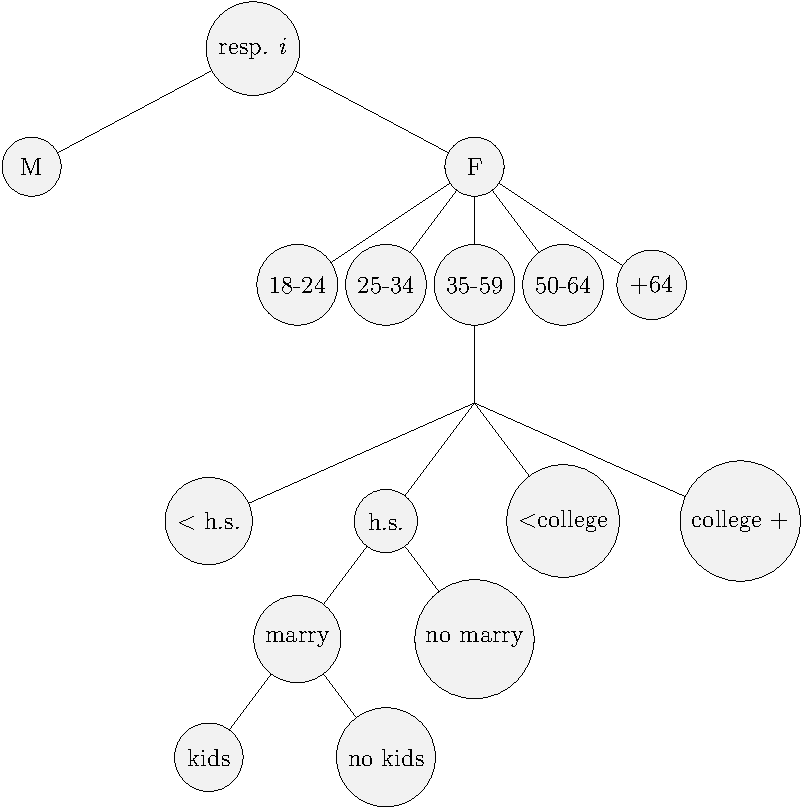
\includegraphics[height = \textwidth, width = \textwidth]{figs/GroupCat}
\end{figure}

The identifying assumption in this paper is that different social and demographic groups have preferences for diverse consumption baskets, which, in turn, influences their inflation expectations. The Michigan survey records a variety of demographic factors as well as the household's Census region. A panel of demographic groups follows the categorization of each of the roughly 273,000 survey responses, from 1978.1-2022.5, into one of 160 categories based on sex, age, education, marital and parental status. Those categories shown in Figure \ref{fig:GroupTree}, produce a panel that consists of $T = 528$ months, $N = 4$ regions, and $G=160$ groups. For each group, additional survey questions serve as controls. These questions include household perceptions of the economy, unemployment, personal income, expected future income, gas price expectations, current household financial status, and expected household financial status. For each period, each region, and each group, the average inflation expectation is treated as the unit of observation.\footnote{The panel dimensions fit a ``small $N$, big $T$'' setting that raises potential finite sample bias concerns that the estimation will address.}

\begin{figure}
\centering
\caption{Group mean price expectations. Groups: men $\leq 80$, women $>80$}\label{fig:GroupMeans}
% Created by tikzDevice version 0.12.3.1 on 2023-10-23 15:56:30
% !TEX encoding = UTF-8 Unicode
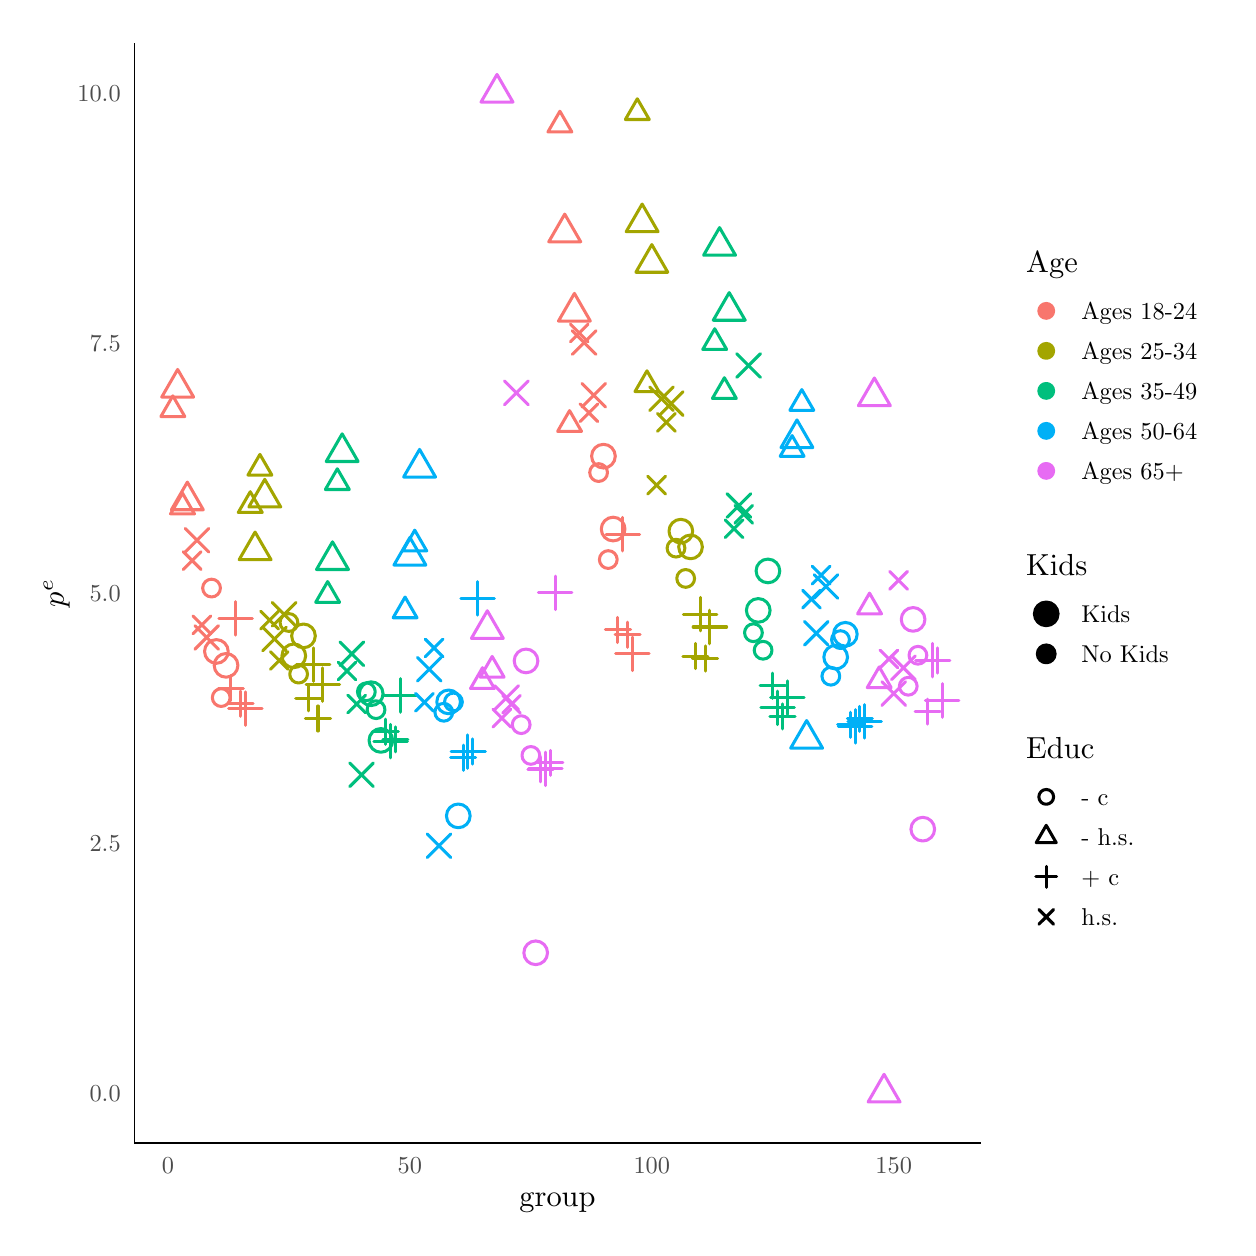
\begin{tikzpicture}[x=1pt,y=1pt]
\definecolor{fillColor}{RGB}{255,255,255}
\path[use as bounding box,fill=fillColor,fill opacity=0.00] (0,0) rectangle (433.62,433.62);
\begin{scope}
\path[clip] ( 38.56, 30.69) rectangle (344.33,428.12);
\definecolor{drawColor}{RGB}{248,118,109}

\path[draw=drawColor,line width= 1.1pt,line join=round,line cap=round] ( 52.45,300.57) --
	( 56.78,293.09) --
	( 48.13,293.09) --
	cycle;

\path[draw=drawColor,line width= 1.1pt,line join=round,line cap=round] ( 54.20,310.11) --
	( 59.97,300.13) --
	( 48.44,300.13) --
	cycle;

\path[draw=drawColor,line width= 1.1pt,line join=round,line cap=round] ( 55.95,265.41) --
	( 60.27,257.92) --
	( 51.63,257.92) --
	cycle;

\path[draw=drawColor,line width= 1.1pt,line join=round,line cap=round] ( 57.70,269.40) --
	( 63.46,259.41) --
	( 51.93,259.41) --
	cycle;

\path[draw=drawColor,line width= 1.1pt,line join=round,line cap=round] ( 56.24,237.85) -- ( 62.66,244.27);

\path[draw=drawColor,line width= 1.1pt,line join=round,line cap=round] ( 56.24,244.27) -- ( 62.66,237.85);

\path[draw=drawColor,line width= 1.1pt,line join=round,line cap=round] ( 56.92,244.13) -- ( 65.48,252.69);

\path[draw=drawColor,line width= 1.1pt,line join=round,line cap=round] ( 56.92,252.69) -- ( 65.48,244.13);

\path[draw=drawColor,line width= 1.1pt,line join=round,line cap=round] ( 59.73,214.58) -- ( 66.15,221.00);

\path[draw=drawColor,line width= 1.1pt,line join=round,line cap=round] ( 59.73,221.00) -- ( 66.15,214.58);

\path[draw=drawColor,line width= 1.1pt,line join=round,line cap=round] ( 60.41,209.00) -- ( 68.97,217.56);

\path[draw=drawColor,line width= 1.1pt,line join=round,line cap=round] ( 60.41,217.56) -- ( 68.97,209.00);

\path[draw=drawColor,line width= 1.1pt,line join=round,line cap=round] ( 66.44,231.12) circle (  3.21);

\path[draw=drawColor,line width= 1.1pt,line join=round,line cap=round] ( 68.19,208.22) circle (  4.28);

\path[draw=drawColor,line width= 1.1pt,line join=round,line cap=round] ( 69.94,191.55) circle (  3.21);

\path[draw=drawColor,line width= 1.1pt,line join=round,line cap=round] ( 71.68,203.19) circle (  4.28);

\path[draw=drawColor,line width= 1.1pt,line join=round,line cap=round] ( 68.89,194.94) -- ( 77.97,194.94);

\path[draw=drawColor,line width= 1.1pt,line join=round,line cap=round] ( 73.43,190.40) -- ( 73.43,199.48);

\path[draw=drawColor,line width= 1.1pt,line join=round,line cap=round] ( 69.13,220.20) -- ( 81.23,220.20);

\path[draw=drawColor,line width= 1.1pt,line join=round,line cap=round] ( 75.18,214.15) -- ( 75.18,226.25);

\path[draw=drawColor,line width= 1.1pt,line join=round,line cap=round] ( 72.39,189.34) -- ( 81.47,189.34);

\path[draw=drawColor,line width= 1.1pt,line join=round,line cap=round] ( 76.93,184.80) -- ( 76.93,193.88);

\path[draw=drawColor,line width= 1.1pt,line join=round,line cap=round] ( 72.63,187.56) -- ( 84.73,187.56);

\path[draw=drawColor,line width= 1.1pt,line join=round,line cap=round] ( 78.68,181.50) -- ( 78.68,193.61);
\definecolor{drawColor}{RGB}{163,165,0}

\path[draw=drawColor,line width= 1.1pt,line join=round,line cap=round] ( 80.43,265.93) --
	( 84.75,258.44) --
	( 76.10,258.44) --
	cycle;

\path[draw=drawColor,line width= 1.1pt,line join=round,line cap=round] ( 82.17,251.35) --
	( 87.94,241.37) --
	( 76.41,241.37) --
	cycle;

\path[draw=drawColor,line width= 1.1pt,line join=round,line cap=round] ( 83.92,279.42) --
	( 88.24,271.94) --
	( 79.60,271.94) --
	cycle;

\path[draw=drawColor,line width= 1.1pt,line join=round,line cap=round] ( 85.67,270.41) --
	( 91.43,260.43) --
	( 79.91,260.43) --
	cycle;

\path[draw=drawColor,line width= 1.1pt,line join=round,line cap=round] ( 84.21,216.33) -- ( 90.63,222.75);

\path[draw=drawColor,line width= 1.1pt,line join=round,line cap=round] ( 84.21,222.75) -- ( 90.63,216.33);

\path[draw=drawColor,line width= 1.1pt,line join=round,line cap=round] ( 84.89,208.45) -- ( 93.45,217.01);

\path[draw=drawColor,line width= 1.1pt,line join=round,line cap=round] ( 84.89,217.01) -- ( 93.45,208.45);

\path[draw=drawColor,line width= 1.1pt,line join=round,line cap=round] ( 87.71,201.74) -- ( 94.12,208.15);

\path[draw=drawColor,line width= 1.1pt,line join=round,line cap=round] ( 87.71,208.15) -- ( 94.12,201.74);

\path[draw=drawColor,line width= 1.1pt,line join=round,line cap=round] ( 88.38,217.36) -- ( 96.94,225.92);

\path[draw=drawColor,line width= 1.1pt,line join=round,line cap=round] ( 88.38,225.92) -- ( 96.94,217.36);

\path[draw=drawColor,line width= 1.1pt,line join=round,line cap=round] ( 94.41,218.67) circle (  3.21);

\path[draw=drawColor,line width= 1.1pt,line join=round,line cap=round] ( 96.16,206.63) circle (  4.28);

\path[draw=drawColor,line width= 1.1pt,line join=round,line cap=round] ( 97.91,200.03) circle (  3.21);

\path[draw=drawColor,line width= 1.1pt,line join=round,line cap=round] ( 99.66,213.84) circle (  4.28);

\path[draw=drawColor,line width= 1.1pt,line join=round,line cap=round] ( 96.87,191.24) -- (105.94,191.24);

\path[draw=drawColor,line width= 1.1pt,line join=round,line cap=round] (101.41,186.71) -- (101.41,195.78);

\path[draw=drawColor,line width= 1.1pt,line join=round,line cap=round] ( 97.10,203.45) -- (109.21,203.45);

\path[draw=drawColor,line width= 1.1pt,line join=round,line cap=round] (103.15,197.40) -- (103.15,209.50);

\path[draw=drawColor,line width= 1.1pt,line join=round,line cap=round] (100.36,183.98) -- (109.44,183.98);

\path[draw=drawColor,line width= 1.1pt,line join=round,line cap=round] (104.90,179.45) -- (104.90,188.52);

\path[draw=drawColor,line width= 1.1pt,line join=round,line cap=round] (100.60,196.22) -- (112.70,196.22);

\path[draw=drawColor,line width= 1.1pt,line join=round,line cap=round] (106.65,190.17) -- (106.65,202.27);
\definecolor{drawColor}{RGB}{0,191,125}

\path[draw=drawColor,line width= 1.1pt,line join=round,line cap=round] (108.40,233.46) --
	(112.72,225.97) --
	(104.08,225.97) --
	cycle;

\path[draw=drawColor,line width= 1.1pt,line join=round,line cap=round] (110.15,247.82) --
	(115.91,237.83) --
	(104.38,237.83) --
	cycle;

\path[draw=drawColor,line width= 1.1pt,line join=round,line cap=round] (111.89,274.22) --
	(116.22,266.73) --
	(107.57,266.73) --
	cycle;

\path[draw=drawColor,line width= 1.1pt,line join=round,line cap=round] (113.64,286.84) --
	(119.41,276.85) --
	(107.88,276.85) --
	cycle;

\path[draw=drawColor,line width= 1.1pt,line join=round,line cap=round] (112.18,197.95) -- (118.60,204.37);

\path[draw=drawColor,line width= 1.1pt,line join=round,line cap=round] (112.18,204.37) -- (118.60,197.95);

\path[draw=drawColor,line width= 1.1pt,line join=round,line cap=round] (112.86,203.09) -- (121.42,211.65);

\path[draw=drawColor,line width= 1.1pt,line join=round,line cap=round] (112.86,211.65) -- (121.42,203.09);

\path[draw=drawColor,line width= 1.1pt,line join=round,line cap=round] (115.68,186.02) -- (122.10,192.44);

\path[draw=drawColor,line width= 1.1pt,line join=round,line cap=round] (115.68,192.44) -- (122.10,186.02);

\path[draw=drawColor,line width= 1.1pt,line join=round,line cap=round] (116.36,159.36) -- (124.92,167.92);

\path[draw=drawColor,line width= 1.1pt,line join=round,line cap=round] (116.36,167.92) -- (124.92,159.36);

\path[draw=drawColor,line width= 1.1pt,line join=round,line cap=round] (122.38,193.64) circle (  3.21);

\path[draw=drawColor,line width= 1.1pt,line join=round,line cap=round] (124.13,192.95) circle (  4.28);

\path[draw=drawColor,line width= 1.1pt,line join=round,line cap=round] (125.88,187.18) circle (  3.21);

\path[draw=drawColor,line width= 1.1pt,line join=round,line cap=round] (127.63,176.07) circle (  4.28);

\path[draw=drawColor,line width= 1.1pt,line join=round,line cap=round] (124.84,179.18) -- (133.92,179.18);

\path[draw=drawColor,line width= 1.1pt,line join=round,line cap=round] (129.38,174.64) -- (129.38,183.72);

\path[draw=drawColor,line width= 1.1pt,line join=round,line cap=round] (125.07,175.84) -- (137.18,175.84);

\path[draw=drawColor,line width= 1.1pt,line join=round,line cap=round] (131.13,169.79) -- (131.13,181.89);

\path[draw=drawColor,line width= 1.1pt,line join=round,line cap=round] (128.34,176.45) -- (137.41,176.45);

\path[draw=drawColor,line width= 1.1pt,line join=round,line cap=round] (132.87,171.91) -- (132.87,180.99);

\path[draw=drawColor,line width= 1.1pt,line join=round,line cap=round] (128.57,192.30) -- (140.68,192.30);

\path[draw=drawColor,line width= 1.1pt,line join=round,line cap=round] (134.62,186.25) -- (134.62,198.36);
\definecolor{drawColor}{RGB}{0,176,246}

\path[draw=drawColor,line width= 1.1pt,line join=round,line cap=round] (136.37,227.87) --
	(140.69,220.39) --
	(132.05,220.39) --
	cycle;

\path[draw=drawColor,line width= 1.1pt,line join=round,line cap=round] (138.12,249.41) --
	(143.88,239.43) --
	(132.35,239.43) --
	cycle;

\path[draw=drawColor,line width= 1.1pt,line join=round,line cap=round] (139.87,252.04) --
	(144.19,244.55) --
	(135.55,244.55) --
	cycle;

\path[draw=drawColor,line width= 1.1pt,line join=round,line cap=round] (141.62,281.22) --
	(147.38,271.24) --
	(135.85,271.24) --
	cycle;

\path[draw=drawColor,line width= 1.1pt,line join=round,line cap=round] (140.15,186.65) -- (146.57,193.06);

\path[draw=drawColor,line width= 1.1pt,line join=round,line cap=round] (140.15,193.06) -- (146.57,186.65);

\path[draw=drawColor,line width= 1.1pt,line join=round,line cap=round] (140.83,197.53) -- (149.39,206.09);

\path[draw=drawColor,line width= 1.1pt,line join=round,line cap=round] (140.83,206.09) -- (149.39,197.53);

\path[draw=drawColor,line width= 1.1pt,line join=round,line cap=round] (143.65,206.26) -- (150.07,212.68);

\path[draw=drawColor,line width= 1.1pt,line join=round,line cap=round] (143.65,212.68) -- (150.07,206.26);

\path[draw=drawColor,line width= 1.1pt,line join=round,line cap=round] (144.33,133.73) -- (152.89,142.29);

\path[draw=drawColor,line width= 1.1pt,line join=round,line cap=round] (144.33,142.29) -- (152.89,133.73);

\path[draw=drawColor,line width= 1.1pt,line join=round,line cap=round] (150.36,186.24) circle (  3.21);

\path[draw=drawColor,line width= 1.1pt,line join=round,line cap=round] (152.11,189.99) circle (  4.28);

\path[draw=drawColor,line width= 1.1pt,line join=round,line cap=round] (153.85,189.97) circle (  3.21);

\path[draw=drawColor,line width= 1.1pt,line join=round,line cap=round] (155.60,148.80) circle (  4.28);

\path[draw=drawColor,line width= 1.1pt,line join=round,line cap=round] (152.81,169.81) -- (161.89,169.81);

\path[draw=drawColor,line width= 1.1pt,line join=round,line cap=round] (157.35,165.27) -- (157.35,174.35);

\path[draw=drawColor,line width= 1.1pt,line join=round,line cap=round] (153.05,172.03) -- (165.15,172.03);

\path[draw=drawColor,line width= 1.1pt,line join=round,line cap=round] (159.10,165.98) -- (159.10,178.08);

\path[draw=drawColor,line width= 1.1pt,line join=round,line cap=round] (156.31,172.06) -- (165.38,172.06);

\path[draw=drawColor,line width= 1.1pt,line join=round,line cap=round] (160.85,167.52) -- (160.85,176.59);

\path[draw=drawColor,line width= 1.1pt,line join=round,line cap=round] (156.54,227.40) -- (168.65,227.40);

\path[draw=drawColor,line width= 1.1pt,line join=round,line cap=round] (162.59,221.34) -- (162.59,233.45);
\definecolor{drawColor}{RGB}{231,107,243}

\path[draw=drawColor,line width= 1.1pt,line join=round,line cap=round] (164.34,202.33) --
	(168.66,194.84) --
	(160.02,194.84) --
	cycle;

\path[draw=drawColor,line width= 1.1pt,line join=round,line cap=round] (166.09,222.92) --
	(171.86,212.94) --
	(160.33,212.94) --
	cycle;

\path[draw=drawColor,line width= 1.1pt,line join=round,line cap=round] (167.84,206.41) --
	(172.16,198.93) --
	(163.52,198.93) --
	cycle;

\path[draw=drawColor,line width= 1.1pt,line join=round,line cap=round] (169.59,416.71) --
	(175.35,406.73) --
	(163.82,406.73) --
	cycle;

\path[draw=drawColor,line width= 1.1pt,line join=round,line cap=round] (168.13,180.90) -- (174.54,187.31);

\path[draw=drawColor,line width= 1.1pt,line join=round,line cap=round] (168.13,187.31) -- (174.54,180.90);

\path[draw=drawColor,line width= 1.1pt,line join=round,line cap=round] (168.80,187.26) -- (177.36,195.82);

\path[draw=drawColor,line width= 1.1pt,line join=round,line cap=round] (168.80,195.82) -- (177.36,187.26);

\path[draw=drawColor,line width= 1.1pt,line join=round,line cap=round] (171.62,185.94) -- (178.04,192.36);

\path[draw=drawColor,line width= 1.1pt,line join=round,line cap=round] (171.62,192.36) -- (178.04,185.94);

\path[draw=drawColor,line width= 1.1pt,line join=round,line cap=round] (172.30,297.38) -- (180.86,305.94);

\path[draw=drawColor,line width= 1.1pt,line join=round,line cap=round] (172.30,305.94) -- (180.86,297.38);

\path[draw=drawColor,line width= 1.1pt,line join=round,line cap=round] (178.33,181.77) circle (  3.21);

\path[draw=drawColor,line width= 1.1pt,line join=round,line cap=round] (180.08,204.79) circle (  4.28);

\path[draw=drawColor,line width= 1.1pt,line join=round,line cap=round] (181.83,170.64) circle (  3.21);

\path[draw=drawColor,line width= 1.1pt,line join=round,line cap=round] (183.57, 99.33) circle (  4.28);

\path[draw=drawColor,line width= 1.1pt,line join=round,line cap=round] (180.78,165.59) -- (189.86,165.59);

\path[draw=drawColor,line width= 1.1pt,line join=round,line cap=round] (185.32,161.05) -- (185.32,170.13);

\path[draw=drawColor,line width= 1.1pt,line join=round,line cap=round] (181.02,165.78) -- (193.12,165.78);

\path[draw=drawColor,line width= 1.1pt,line join=round,line cap=round] (187.07,159.73) -- (187.07,171.83);

\path[draw=drawColor,line width= 1.1pt,line join=round,line cap=round] (184.28,167.94) -- (193.36,167.94);

\path[draw=drawColor,line width= 1.1pt,line join=round,line cap=round] (188.82,163.40) -- (188.82,172.48);

\path[draw=drawColor,line width= 1.1pt,line join=round,line cap=round] (184.51,229.40) -- (196.62,229.40);

\path[draw=drawColor,line width= 1.1pt,line join=round,line cap=round] (190.57,223.35) -- (190.57,235.46);
\definecolor{drawColor}{RGB}{248,118,109}

\path[draw=drawColor,line width= 1.1pt,line join=round,line cap=round] (192.32,403.42) --
	(196.64,395.93) --
	(187.99,395.93) --
	cycle;

\path[draw=drawColor,line width= 1.1pt,line join=round,line cap=round] (194.06,366.24) --
	(199.83,356.25) --
	(188.30,356.25) --
	cycle;

\path[draw=drawColor,line width= 1.1pt,line join=round,line cap=round] (195.81,295.23) --
	(200.13,287.74) --
	(191.49,287.74) --
	cycle;

\path[draw=drawColor,line width= 1.1pt,line join=round,line cap=round] (197.56,337.59) --
	(203.32,327.60) --
	(191.80,327.60) --
	cycle;

\path[draw=drawColor,line width= 1.1pt,line join=round,line cap=round] (196.10,320.10) -- (202.52,326.52);

\path[draw=drawColor,line width= 1.1pt,line join=round,line cap=round] (196.10,326.52) -- (202.52,320.10);

\path[draw=drawColor,line width= 1.1pt,line join=round,line cap=round] (196.78,315.55) -- (205.34,324.11);

\path[draw=drawColor,line width= 1.1pt,line join=round,line cap=round] (196.78,324.11) -- (205.34,315.55);

\path[draw=drawColor,line width= 1.1pt,line join=round,line cap=round] (199.60,291.25) -- (206.01,297.67);

\path[draw=drawColor,line width= 1.1pt,line join=round,line cap=round] (199.60,297.67) -- (206.01,291.25);

\path[draw=drawColor,line width= 1.1pt,line join=round,line cap=round] (200.27,296.54) -- (208.83,305.10);

\path[draw=drawColor,line width= 1.1pt,line join=round,line cap=round] (200.27,305.10) -- (208.83,296.54);

\path[draw=drawColor,line width= 1.1pt,line join=round,line cap=round] (206.30,272.86) circle (  3.21);

\path[draw=drawColor,line width= 1.1pt,line join=round,line cap=round] (208.05,278.78) circle (  4.28);

\path[draw=drawColor,line width= 1.1pt,line join=round,line cap=round] (209.80,241.42) circle (  3.21);

\path[draw=drawColor,line width= 1.1pt,line join=round,line cap=round] (211.55,252.44) circle (  4.28);

\path[draw=drawColor,line width= 1.1pt,line join=round,line cap=round] (208.76,215.98) -- (217.83,215.98);

\path[draw=drawColor,line width= 1.1pt,line join=round,line cap=round] (213.29,211.45) -- (213.29,220.52);

\path[draw=drawColor,line width= 1.1pt,line join=round,line cap=round] (208.99,250.58) -- (221.10,250.58);

\path[draw=drawColor,line width= 1.1pt,line join=round,line cap=round] (215.04,244.52) -- (215.04,256.63);

\path[draw=drawColor,line width= 1.1pt,line join=round,line cap=round] (212.25,214.26) -- (221.33,214.26);

\path[draw=drawColor,line width= 1.1pt,line join=round,line cap=round] (216.79,209.73) -- (216.79,218.80);

\path[draw=drawColor,line width= 1.1pt,line join=round,line cap=round] (212.49,207.36) -- (224.59,207.36);

\path[draw=drawColor,line width= 1.1pt,line join=round,line cap=round] (218.54,201.30) -- (218.54,213.41);
\definecolor{drawColor}{RGB}{163,165,0}

\path[draw=drawColor,line width= 1.1pt,line join=round,line cap=round] (220.29,407.92) --
	(224.61,400.43) --
	(215.97,400.43) --
	cycle;

\path[draw=drawColor,line width= 1.1pt,line join=round,line cap=round] (222.04,369.88) --
	(227.80,359.90) --
	(216.27,359.90) --
	cycle;

\path[draw=drawColor,line width= 1.1pt,line join=round,line cap=round] (223.78,309.62) --
	(228.11,302.13) --
	(219.46,302.13) --
	cycle;

\path[draw=drawColor,line width= 1.1pt,line join=round,line cap=round] (225.53,355.22) --
	(231.30,345.24) --
	(219.77,345.24) --
	cycle;

\path[draw=drawColor,line width= 1.1pt,line join=round,line cap=round] (224.07,265.10) -- (230.49,271.52);

\path[draw=drawColor,line width= 1.1pt,line join=round,line cap=round] (224.07,271.52) -- (230.49,265.10);

\path[draw=drawColor,line width= 1.1pt,line join=round,line cap=round] (224.75,295.22) -- (233.31,303.78);

\path[draw=drawColor,line width= 1.1pt,line join=round,line cap=round] (224.75,303.78) -- (233.31,295.22);

\path[draw=drawColor,line width= 1.1pt,line join=round,line cap=round] (227.57,287.76) -- (233.99,294.18);

\path[draw=drawColor,line width= 1.1pt,line join=round,line cap=round] (227.57,294.18) -- (233.99,287.76);

\path[draw=drawColor,line width= 1.1pt,line join=round,line cap=round] (228.25,293.50) -- (236.81,302.06);

\path[draw=drawColor,line width= 1.1pt,line join=round,line cap=round] (228.25,302.06) -- (236.81,293.50);

\path[draw=drawColor,line width= 1.1pt,line join=round,line cap=round] (234.27,245.54) circle (  3.21);

\path[draw=drawColor,line width= 1.1pt,line join=round,line cap=round] (236.02,251.68) circle (  4.28);

\path[draw=drawColor,line width= 1.1pt,line join=round,line cap=round] (237.77,234.60) circle (  3.21);

\path[draw=drawColor,line width= 1.1pt,line join=round,line cap=round] (239.52,245.99) circle (  4.28);

\path[draw=drawColor,line width= 1.1pt,line join=round,line cap=round] (236.73,206.56) -- (245.80,206.56);

\path[draw=drawColor,line width= 1.1pt,line join=round,line cap=round] (241.27,202.02) -- (241.27,211.10);

\path[draw=drawColor,line width= 1.1pt,line join=round,line cap=round] (236.96,221.72) -- (249.07,221.72);

\path[draw=drawColor,line width= 1.1pt,line join=round,line cap=round] (243.01,215.66) -- (243.01,227.77);

\path[draw=drawColor,line width= 1.1pt,line join=round,line cap=round] (240.23,205.65) -- (249.30,205.65);

\path[draw=drawColor,line width= 1.1pt,line join=round,line cap=round] (244.76,201.11) -- (244.76,210.19);

\path[draw=drawColor,line width= 1.1pt,line join=round,line cap=round] (240.46,217.05) -- (252.56,217.05);

\path[draw=drawColor,line width= 1.1pt,line join=round,line cap=round] (246.51,211.00) -- (246.51,223.10);
\definecolor{drawColor}{RGB}{0,191,125}

\path[draw=drawColor,line width= 1.1pt,line join=round,line cap=round] (248.26,324.82) --
	(252.58,317.34) --
	(243.94,317.34) --
	cycle;

\path[draw=drawColor,line width= 1.1pt,line join=round,line cap=round] (250.01,361.37) --
	(255.77,351.39) --
	(244.24,351.39) --
	cycle;

\path[draw=drawColor,line width= 1.1pt,line join=round,line cap=round] (251.76,307.12) --
	(256.08,299.64) --
	(247.43,299.64) --
	cycle;

\path[draw=drawColor,line width= 1.1pt,line join=round,line cap=round] (253.50,337.88) --
	(259.27,327.90) --
	(247.74,327.90) --
	cycle;

\path[draw=drawColor,line width= 1.1pt,line join=round,line cap=round] (252.04,249.33) -- (258.46,255.75);

\path[draw=drawColor,line width= 1.1pt,line join=round,line cap=round] (252.04,255.75) -- (258.46,249.33);

\path[draw=drawColor,line width= 1.1pt,line join=round,line cap=round] (252.72,256.67) -- (261.28,265.23);

\path[draw=drawColor,line width= 1.1pt,line join=round,line cap=round] (252.72,265.23) -- (261.28,256.67);

\path[draw=drawColor,line width= 1.1pt,line join=round,line cap=round] (255.54,254.56) -- (261.96,260.98);

\path[draw=drawColor,line width= 1.1pt,line join=round,line cap=round] (255.54,260.98) -- (261.96,254.56);

\path[draw=drawColor,line width= 1.1pt,line join=round,line cap=round] (256.22,307.25) -- (264.78,315.81);

\path[draw=drawColor,line width= 1.1pt,line join=round,line cap=round] (256.22,315.81) -- (264.78,307.25);

\path[draw=drawColor,line width= 1.1pt,line join=round,line cap=round] (262.25,214.98) circle (  3.21);

\path[draw=drawColor,line width= 1.1pt,line join=round,line cap=round] (263.99,223.05) circle (  4.28);

\path[draw=drawColor,line width= 1.1pt,line join=round,line cap=round] (265.74,208.65) circle (  3.21);

\path[draw=drawColor,line width= 1.1pt,line join=round,line cap=round] (267.49,237.31) circle (  4.28);

\path[draw=drawColor,line width= 1.1pt,line join=round,line cap=round] (264.70,195.84) -- (273.78,195.84);

\path[draw=drawColor,line width= 1.1pt,line join=round,line cap=round] (269.24,191.30) -- (269.24,200.37);

\path[draw=drawColor,line width= 1.1pt,line join=round,line cap=round] (264.93,187.80) -- (277.04,187.80);

\path[draw=drawColor,line width= 1.1pt,line join=round,line cap=round] (270.99,181.75) -- (270.99,193.85);

\path[draw=drawColor,line width= 1.1pt,line join=round,line cap=round] (268.20,184.73) -- (277.27,184.73);

\path[draw=drawColor,line width= 1.1pt,line join=round,line cap=round] (272.74,180.20) -- (272.74,189.27);

\path[draw=drawColor,line width= 1.1pt,line join=round,line cap=round] (268.43,191.51) -- (280.54,191.51);

\path[draw=drawColor,line width= 1.1pt,line join=round,line cap=round] (274.48,185.45) -- (274.48,197.56);
\definecolor{drawColor}{RGB}{0,176,246}

\path[draw=drawColor,line width= 1.1pt,line join=round,line cap=round] (276.23,286.22) --
	(280.55,278.73) --
	(271.91,278.73) --
	cycle;

\path[draw=drawColor,line width= 1.1pt,line join=round,line cap=round] (277.98,291.87) --
	(283.74,281.89) --
	(272.22,281.89) --
	cycle;

\path[draw=drawColor,line width= 1.1pt,line join=round,line cap=round] (279.73,302.83) --
	(284.05,295.35) --
	(275.41,295.35) --
	cycle;

\path[draw=drawColor,line width= 1.1pt,line join=round,line cap=round] (281.48,183.25) --
	(287.24,173.27) --
	(275.71,173.27) --
	cycle;

\path[draw=drawColor,line width= 1.1pt,line join=round,line cap=round] (280.02,223.91) -- (286.43,230.33);

\path[draw=drawColor,line width= 1.1pt,line join=round,line cap=round] (280.02,230.33) -- (286.43,223.91);

\path[draw=drawColor,line width= 1.1pt,line join=round,line cap=round] (280.69,210.49) -- (289.25,219.04);

\path[draw=drawColor,line width= 1.1pt,line join=round,line cap=round] (280.69,219.04) -- (289.25,210.49);

\path[draw=drawColor,line width= 1.1pt,line join=round,line cap=round] (283.51,232.58) -- (289.93,239.00);

\path[draw=drawColor,line width= 1.1pt,line join=round,line cap=round] (283.51,239.00) -- (289.93,232.58);

\path[draw=drawColor,line width= 1.1pt,line join=round,line cap=round] (284.19,227.38) -- (292.75,235.94);

\path[draw=drawColor,line width= 1.1pt,line join=round,line cap=round] (284.19,235.94) -- (292.75,227.38);

\path[draw=drawColor,line width= 1.1pt,line join=round,line cap=round] (290.22,199.27) circle (  3.21);

\path[draw=drawColor,line width= 1.1pt,line join=round,line cap=round] (291.97,206.16) circle (  4.28);

\path[draw=drawColor,line width= 1.1pt,line join=round,line cap=round] (293.71,212.49) circle (  3.21);

\path[draw=drawColor,line width= 1.1pt,line join=round,line cap=round] (295.46,214.42) circle (  4.28);

\path[draw=drawColor,line width= 1.1pt,line join=round,line cap=round] (292.67,181.70) -- (301.75,181.70);

\path[draw=drawColor,line width= 1.1pt,line join=round,line cap=round] (297.21,177.16) -- (297.21,186.24);

\path[draw=drawColor,line width= 1.1pt,line join=round,line cap=round] (292.91,181.16) -- (305.01,181.16);

\path[draw=drawColor,line width= 1.1pt,line join=round,line cap=round] (298.96,175.11) -- (298.96,187.22);

\path[draw=drawColor,line width= 1.1pt,line join=round,line cap=round] (296.17,183.86) -- (305.25,183.86);

\path[draw=drawColor,line width= 1.1pt,line join=round,line cap=round] (300.71,179.33) -- (300.71,188.40);

\path[draw=drawColor,line width= 1.1pt,line join=round,line cap=round] (296.40,182.95) -- (308.51,182.95);

\path[draw=drawColor,line width= 1.1pt,line join=round,line cap=round] (302.46,176.90) -- (302.46,189.00);
\definecolor{drawColor}{RGB}{231,107,243}

\path[draw=drawColor,line width= 1.1pt,line join=round,line cap=round] (304.20,229.29) --
	(308.53,221.80) --
	(299.88,221.80) --
	cycle;

\path[draw=drawColor,line width= 1.1pt,line join=round,line cap=round] (305.95,307.02) --
	(311.72,297.03) --
	(300.19,297.03) --
	cycle;

\path[draw=drawColor,line width= 1.1pt,line join=round,line cap=round] (307.70,202.63) --
	(312.02,195.15) --
	(303.38,195.15) --
	cycle;

\path[draw=drawColor,line width= 1.1pt,line join=round,line cap=round] (309.45, 55.41) --
	(315.21, 45.42) --
	(303.69, 45.42) --
	cycle;

\path[draw=drawColor,line width= 1.1pt,line join=round,line cap=round] (307.99,202.29) -- (314.41,208.70);

\path[draw=drawColor,line width= 1.1pt,line join=round,line cap=round] (307.99,208.70) -- (314.41,202.29);

\path[draw=drawColor,line width= 1.1pt,line join=round,line cap=round] (308.67,188.71) -- (317.23,197.27);

\path[draw=drawColor,line width= 1.1pt,line join=round,line cap=round] (308.67,197.27) -- (317.23,188.71);

\path[draw=drawColor,line width= 1.1pt,line join=round,line cap=round] (311.49,230.71) -- (317.90,237.13);

\path[draw=drawColor,line width= 1.1pt,line join=round,line cap=round] (311.49,237.13) -- (317.90,230.71);

\path[draw=drawColor,line width= 1.1pt,line join=round,line cap=round] (312.16,198.03) -- (320.72,206.59);

\path[draw=drawColor,line width= 1.1pt,line join=round,line cap=round] (312.16,206.59) -- (320.72,198.03);

\path[draw=drawColor,line width= 1.1pt,line join=round,line cap=round] (318.19,195.64) circle (  3.21);

\path[draw=drawColor,line width= 1.1pt,line join=round,line cap=round] (319.94,219.80) circle (  4.28);

\path[draw=drawColor,line width= 1.1pt,line join=round,line cap=round] (321.69,206.84) circle (  3.21);

\path[draw=drawColor,line width= 1.1pt,line join=round,line cap=round] (323.44,144.00) circle (  4.28);

\path[draw=drawColor,line width= 1.1pt,line join=round,line cap=round] (320.65,186.47) -- (329.72,186.47);

\path[draw=drawColor,line width= 1.1pt,line join=round,line cap=round] (325.18,181.94) -- (325.18,191.01);

\path[draw=drawColor,line width= 1.1pt,line join=round,line cap=round] (320.88,205.04) -- (332.98,205.04);

\path[draw=drawColor,line width= 1.1pt,line join=round,line cap=round] (326.93,198.99) -- (326.93,211.09);

\path[draw=drawColor,line width= 1.1pt,line join=round,line cap=round] (324.14,204.94) -- (333.22,204.94);

\path[draw=drawColor,line width= 1.1pt,line join=round,line cap=round] (328.68,200.40) -- (328.68,209.48);

\path[draw=drawColor,line width= 1.1pt,line join=round,line cap=round] (324.38,190.49) -- (336.48,190.49);

\path[draw=drawColor,line width= 1.1pt,line join=round,line cap=round] (330.43,184.44) -- (330.43,196.55);
\end{scope}
\begin{scope}
\path[clip] (  0.00,  0.00) rectangle (433.62,433.62);
\definecolor{drawColor}{RGB}{0,0,0}

\path[draw=drawColor,line width= 0.6pt,line join=round] ( 38.56, 30.69) --
	( 38.56,428.12);
\end{scope}
\begin{scope}
\path[clip] (  0.00,  0.00) rectangle (433.62,433.62);
\definecolor{drawColor}{gray}{0.30}

\node[text=drawColor,anchor=base east,inner sep=0pt, outer sep=0pt, scale=  0.88] at ( 33.61, 45.72) {0.0};

\node[text=drawColor,anchor=base east,inner sep=0pt, outer sep=0pt, scale=  0.88] at ( 33.61,136.05) {2.5};

\node[text=drawColor,anchor=base east,inner sep=0pt, outer sep=0pt, scale=  0.88] at ( 33.61,226.37) {5.0};

\node[text=drawColor,anchor=base east,inner sep=0pt, outer sep=0pt, scale=  0.88] at ( 33.61,316.70) {7.5};

\node[text=drawColor,anchor=base east,inner sep=0pt, outer sep=0pt, scale=  0.88] at ( 33.61,407.02) {10.0};
\end{scope}
\begin{scope}
\path[clip] (  0.00,  0.00) rectangle (433.62,433.62);
\definecolor{drawColor}{RGB}{0,0,0}

\path[draw=drawColor,line width= 0.6pt,line join=round] ( 38.56, 30.69) --
	(344.33, 30.69);
\end{scope}
\begin{scope}
\path[clip] (  0.00,  0.00) rectangle (433.62,433.62);
\definecolor{drawColor}{gray}{0.30}

\node[text=drawColor,anchor=base,inner sep=0pt, outer sep=0pt, scale=  0.88] at ( 50.71, 19.68) {0};

\node[text=drawColor,anchor=base,inner sep=0pt, outer sep=0pt, scale=  0.88] at (138.12, 19.68) {50};

\node[text=drawColor,anchor=base,inner sep=0pt, outer sep=0pt, scale=  0.88] at (225.53, 19.68) {100};

\node[text=drawColor,anchor=base,inner sep=0pt, outer sep=0pt, scale=  0.88] at (312.95, 19.68) {150};
\end{scope}
\begin{scope}
\path[clip] (  0.00,  0.00) rectangle (433.62,433.62);
\definecolor{drawColor}{RGB}{0,0,0}

\node[text=drawColor,anchor=base,inner sep=0pt, outer sep=0pt, scale=  1.10] at (191.44,  7.64) {group};
\end{scope}
\begin{scope}
\path[clip] (  0.00,  0.00) rectangle (433.62,433.62);
\definecolor{drawColor}{RGB}{0,0,0}

\node[text=drawColor,rotate= 90.00,anchor=base,inner sep=0pt, outer sep=0pt, scale=  1.10] at ( 13.08,229.40) {$p^e$};
\end{scope}
\begin{scope}
\path[clip] (  0.00,  0.00) rectangle (433.62,433.62);
\definecolor{drawColor}{RGB}{0,0,0}

\node[text=drawColor,anchor=base west,inner sep=0pt, outer sep=0pt, scale=  1.10] at (360.83,345.08) {Age};
\end{scope}
\begin{scope}
\path[clip] (  0.00,  0.00) rectangle (433.62,433.62);
\definecolor{drawColor}{RGB}{248,118,109}
\definecolor{fillColor}{RGB}{248,118,109}

\path[draw=drawColor,line width= 1.1pt,line join=round,line cap=round,fill=fillColor] (368.05,331.28) circle (  2.67);
\end{scope}
\begin{scope}
\path[clip] (  0.00,  0.00) rectangle (433.62,433.62);
\definecolor{drawColor}{RGB}{163,165,0}
\definecolor{fillColor}{RGB}{163,165,0}

\path[draw=drawColor,line width= 1.1pt,line join=round,line cap=round,fill=fillColor] (368.05,316.83) circle (  2.67);
\end{scope}
\begin{scope}
\path[clip] (  0.00,  0.00) rectangle (433.62,433.62);
\definecolor{drawColor}{RGB}{0,191,125}
\definecolor{fillColor}{RGB}{0,191,125}

\path[draw=drawColor,line width= 1.1pt,line join=round,line cap=round,fill=fillColor] (368.05,302.37) circle (  2.67);
\end{scope}
\begin{scope}
\path[clip] (  0.00,  0.00) rectangle (433.62,433.62);
\definecolor{drawColor}{RGB}{0,176,246}
\definecolor{fillColor}{RGB}{0,176,246}

\path[draw=drawColor,line width= 1.1pt,line join=round,line cap=round,fill=fillColor] (368.05,287.92) circle (  2.67);
\end{scope}
\begin{scope}
\path[clip] (  0.00,  0.00) rectangle (433.62,433.62);
\definecolor{drawColor}{RGB}{231,107,243}
\definecolor{fillColor}{RGB}{231,107,243}

\path[draw=drawColor,line width= 1.1pt,line join=round,line cap=round,fill=fillColor] (368.05,273.46) circle (  2.67);
\end{scope}
\begin{scope}
\path[clip] (  0.00,  0.00) rectangle (433.62,433.62);
\definecolor{drawColor}{RGB}{0,0,0}

\node[text=drawColor,anchor=base west,inner sep=0pt, outer sep=0pt, scale=  0.88] at (380.78,328.25) {Ages 18-24};
\end{scope}
\begin{scope}
\path[clip] (  0.00,  0.00) rectangle (433.62,433.62);
\definecolor{drawColor}{RGB}{0,0,0}

\node[text=drawColor,anchor=base west,inner sep=0pt, outer sep=0pt, scale=  0.88] at (380.78,313.80) {Ages 25-34};
\end{scope}
\begin{scope}
\path[clip] (  0.00,  0.00) rectangle (433.62,433.62);
\definecolor{drawColor}{RGB}{0,0,0}

\node[text=drawColor,anchor=base west,inner sep=0pt, outer sep=0pt, scale=  0.88] at (380.78,299.34) {Ages 35-49};
\end{scope}
\begin{scope}
\path[clip] (  0.00,  0.00) rectangle (433.62,433.62);
\definecolor{drawColor}{RGB}{0,0,0}

\node[text=drawColor,anchor=base west,inner sep=0pt, outer sep=0pt, scale=  0.88] at (380.78,284.89) {Ages 50-64};
\end{scope}
\begin{scope}
\path[clip] (  0.00,  0.00) rectangle (433.62,433.62);
\definecolor{drawColor}{RGB}{0,0,0}

\node[text=drawColor,anchor=base west,inner sep=0pt, outer sep=0pt, scale=  0.88] at (380.78,270.43) {Ages 65+};
\end{scope}
\begin{scope}
\path[clip] (  0.00,  0.00) rectangle (433.62,433.62);
\definecolor{drawColor}{RGB}{0,0,0}

\node[text=drawColor,anchor=base west,inner sep=0pt, outer sep=0pt, scale=  1.10] at (360.83,235.59) {Kids};
\end{scope}
\begin{scope}
\path[clip] (  0.00,  0.00) rectangle (433.62,433.62);
\definecolor{drawColor}{RGB}{0,0,0}
\definecolor{fillColor}{RGB}{0,0,0}

\path[draw=drawColor,line width= 1.1pt,line join=round,line cap=round,fill=fillColor] (368.05,221.80) circle (  4.28);
\end{scope}
\begin{scope}
\path[clip] (  0.00,  0.00) rectangle (433.62,433.62);
\definecolor{drawColor}{RGB}{0,0,0}
\definecolor{fillColor}{RGB}{0,0,0}

\path[draw=drawColor,line width= 1.1pt,line join=round,line cap=round,fill=fillColor] (368.05,207.34) circle (  3.21);
\end{scope}
\begin{scope}
\path[clip] (  0.00,  0.00) rectangle (433.62,433.62);
\definecolor{drawColor}{RGB}{0,0,0}

\node[text=drawColor,anchor=base west,inner sep=0pt, outer sep=0pt, scale=  0.88] at (380.78,218.77) {Kids};
\end{scope}
\begin{scope}
\path[clip] (  0.00,  0.00) rectangle (433.62,433.62);
\definecolor{drawColor}{RGB}{0,0,0}

\node[text=drawColor,anchor=base west,inner sep=0pt, outer sep=0pt, scale=  0.88] at (380.78,204.31) {No Kids};
\end{scope}
\begin{scope}
\path[clip] (  0.00,  0.00) rectangle (433.62,433.62);
\definecolor{drawColor}{RGB}{0,0,0}

\node[text=drawColor,anchor=base west,inner sep=0pt, outer sep=0pt, scale=  1.10] at (360.83,169.47) {Educ};
\end{scope}
\begin{scope}
\path[clip] (  0.00,  0.00) rectangle (433.62,433.62);
\definecolor{drawColor}{RGB}{0,0,0}

\path[draw=drawColor,line width= 1.1pt,line join=round,line cap=round] (368.05,155.67) circle (  2.67);
\end{scope}
\begin{scope}
\path[clip] (  0.00,  0.00) rectangle (433.62,433.62);
\definecolor{drawColor}{RGB}{0,0,0}

\path[draw=drawColor,line width= 1.1pt,line join=round,line cap=round] (368.05,145.38) --
	(371.65,139.14) --
	(364.45,139.14) --
	cycle;
\end{scope}
\begin{scope}
\path[clip] (  0.00,  0.00) rectangle (433.62,433.62);
\definecolor{drawColor}{RGB}{0,0,0}

\path[draw=drawColor,line width= 1.1pt,line join=round,line cap=round] (364.27,126.77) -- (371.83,126.77);

\path[draw=drawColor,line width= 1.1pt,line join=round,line cap=round] (368.05,122.98) -- (368.05,130.55);
\end{scope}
\begin{scope}
\path[clip] (  0.00,  0.00) rectangle (433.62,433.62);
\definecolor{drawColor}{RGB}{0,0,0}

\path[draw=drawColor,line width= 1.1pt,line join=round,line cap=round] (365.38,109.64) -- (370.73,114.98);

\path[draw=drawColor,line width= 1.1pt,line join=round,line cap=round] (365.38,114.98) -- (370.73,109.64);
\end{scope}
\begin{scope}
\path[clip] (  0.00,  0.00) rectangle (433.62,433.62);
\definecolor{drawColor}{RGB}{0,0,0}

\node[text=drawColor,anchor=base west,inner sep=0pt, outer sep=0pt, scale=  0.88] at (380.78,152.64) {- c};
\end{scope}
\begin{scope}
\path[clip] (  0.00,  0.00) rectangle (433.62,433.62);
\definecolor{drawColor}{RGB}{0,0,0}

\node[text=drawColor,anchor=base west,inner sep=0pt, outer sep=0pt, scale=  0.88] at (380.78,138.19) {- h.s.};
\end{scope}
\begin{scope}
\path[clip] (  0.00,  0.00) rectangle (433.62,433.62);
\definecolor{drawColor}{RGB}{0,0,0}

\node[text=drawColor,anchor=base west,inner sep=0pt, outer sep=0pt, scale=  0.88] at (380.78,123.74) {+ c};
\end{scope}
\begin{scope}
\path[clip] (  0.00,  0.00) rectangle (433.62,433.62);
\definecolor{drawColor}{RGB}{0,0,0}

\node[text=drawColor,anchor=base west,inner sep=0pt, outer sep=0pt, scale=  0.88] at (380.78,109.28) {h.s.};
\end{scope}
\end{tikzpicture}

\end{figure}

Figure \ref{fig:GroupMeans} provides the first snapshot of the variation exploited by the quasi-experimental design. Each point represents a particular demographic group's mean inflation expectations, averaged across regions and time. Groups below 80 are men, and above are women. Each age group and education level has its color and shape, and women's higher average inflation expectations are apparent. The figure also illustrates heterogeneity across age and schooling.

There is substantial variation in inflation expectations across time, geographic regions, and demographic groups. Figure \ref{fig:intro} documents the gender variation in the Michigan survey data. The panel illustrates the notable difference in inflation expectations by men and women (\cite{BryanVenkatu}). Outside of the high inflation during the 1970s and subsequent disinflation, women tend to expect higher inflation rates. Panel (b) plots the contribution of each region to an unweighted average inflation expectation, with periods of significant disparity.  



\begin{figure}
\centering
\caption{Diversity of inflation survey expectations: gender \& regions.}\label{fig:intro}
\begin{subfigure}[t]{ 0.75\textwidth}
\centering
%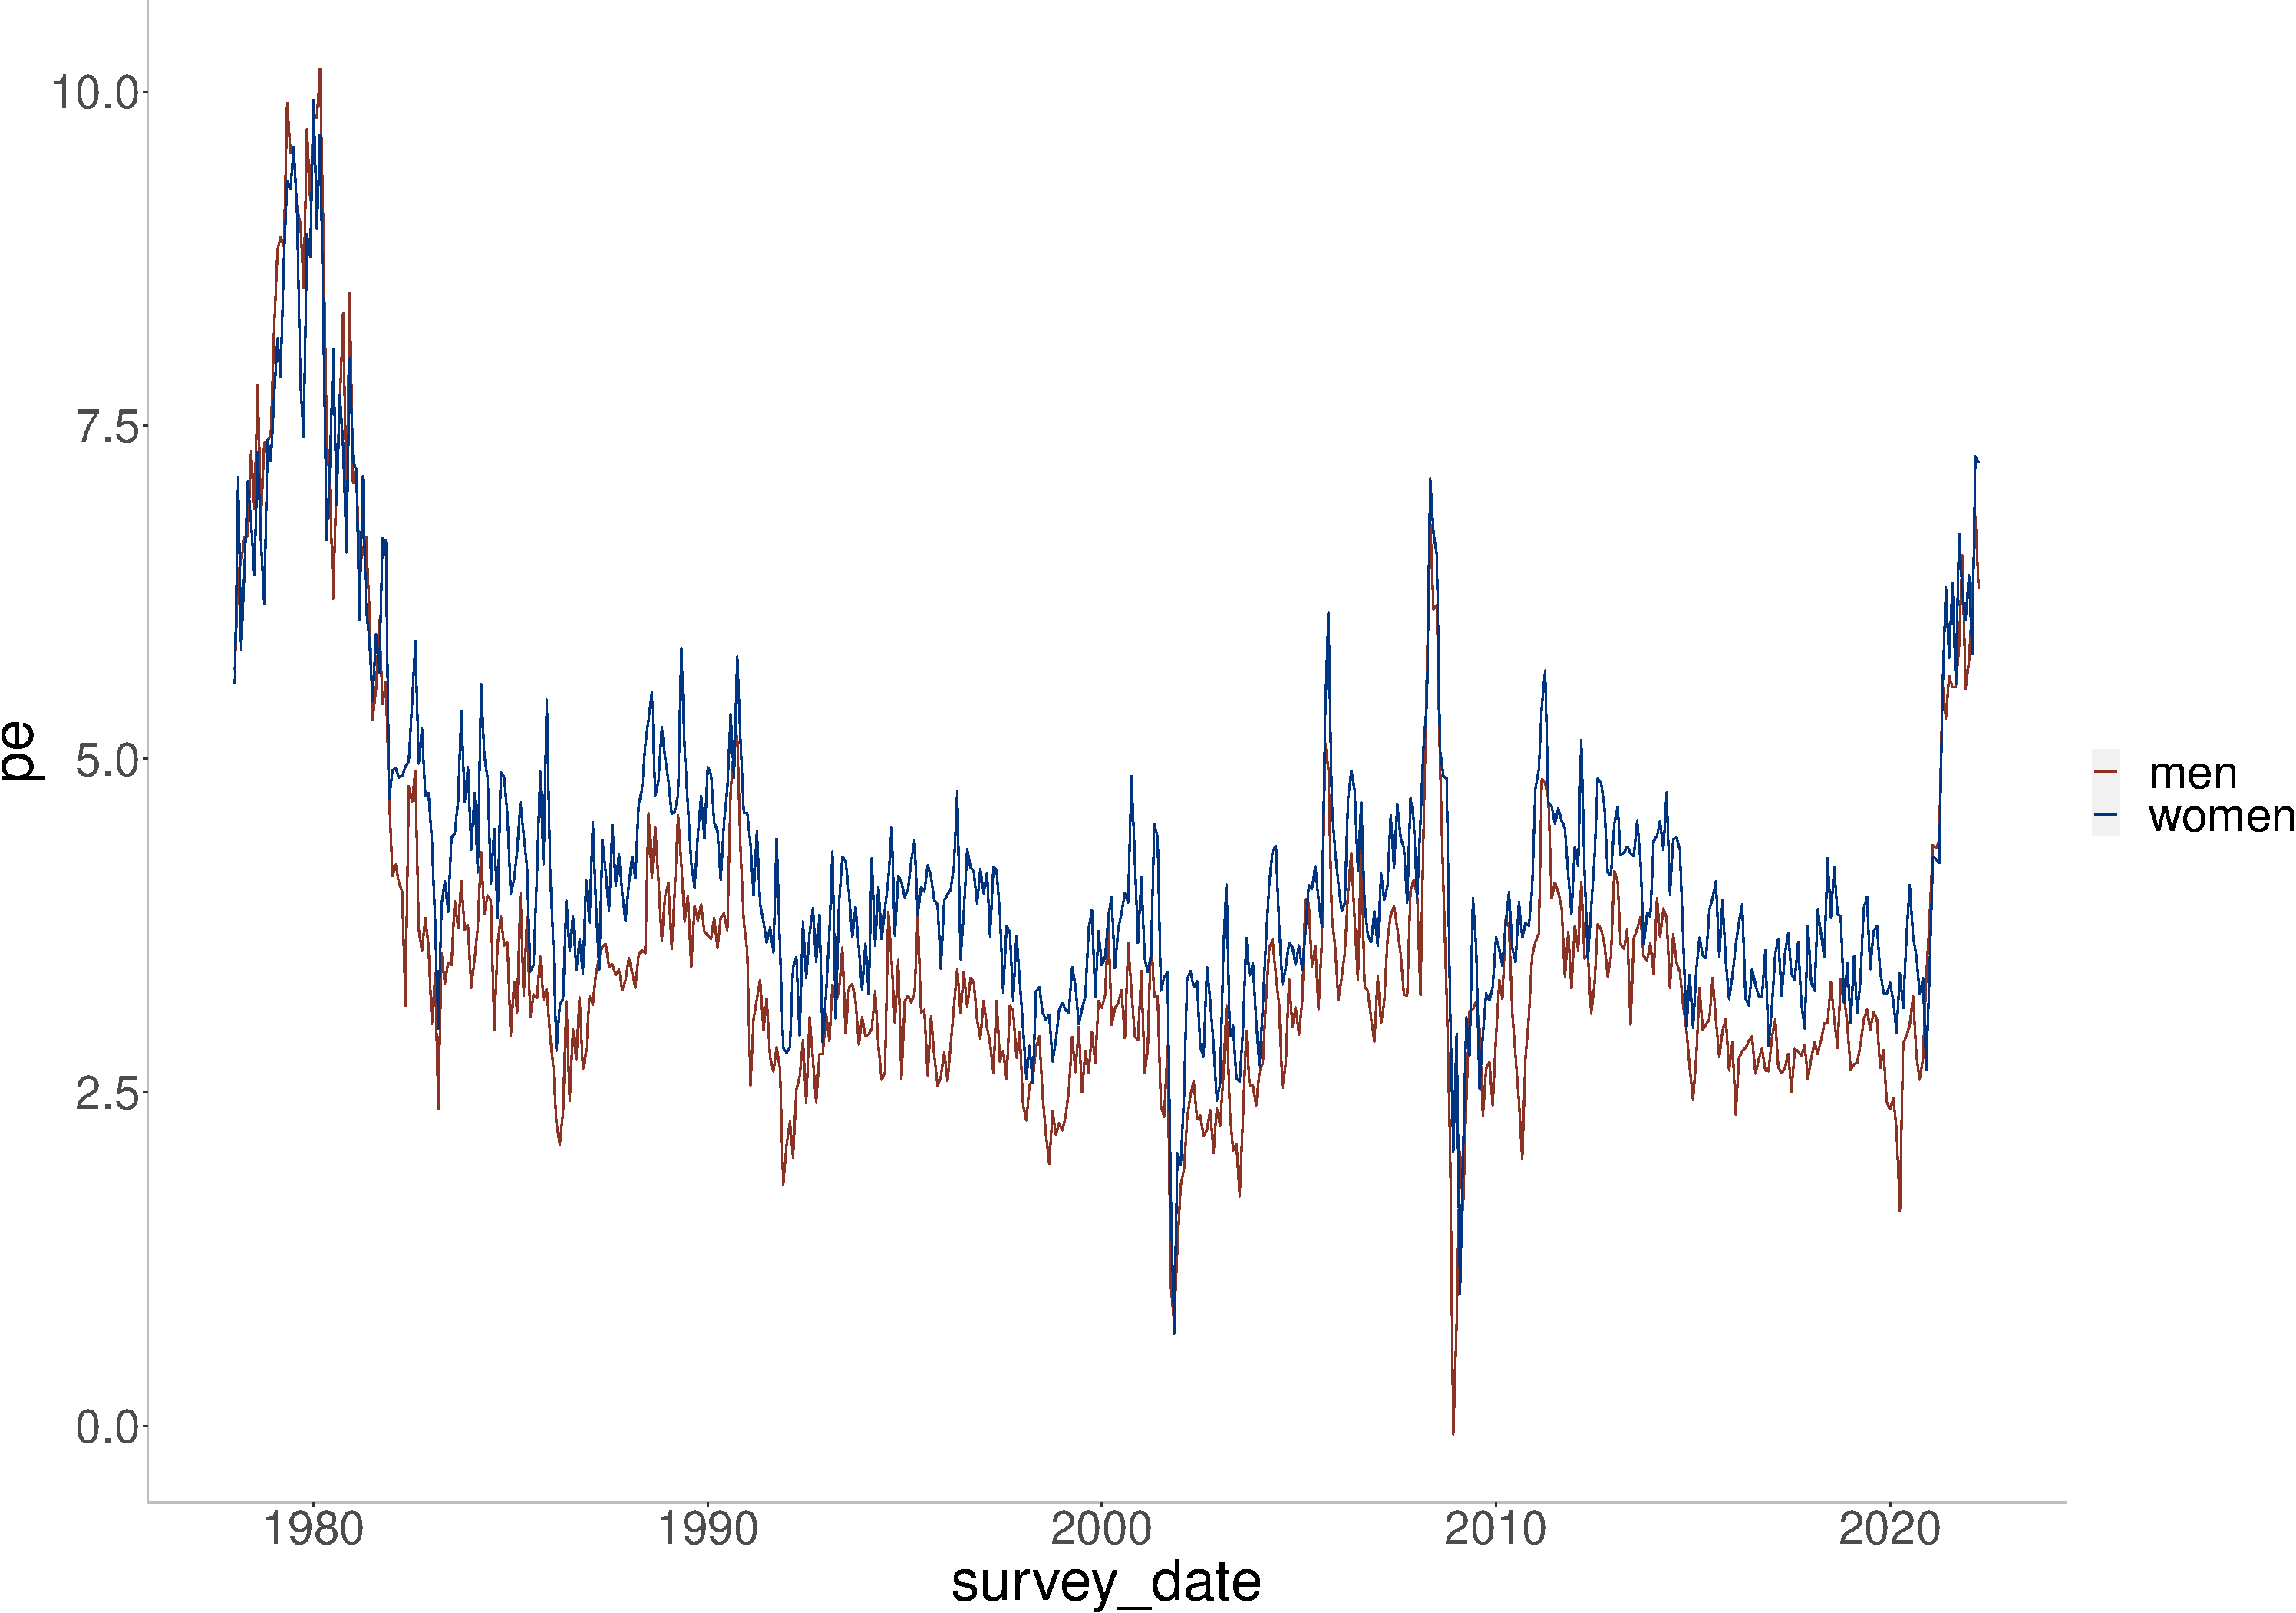
\includegraphics[width = 3in, height =2in]{figs/menwomen}
% Created by tikzDevice version 0.12.3.1 on 2023-10-23 15:56:04
% !TEX encoding = UTF-8 Unicode
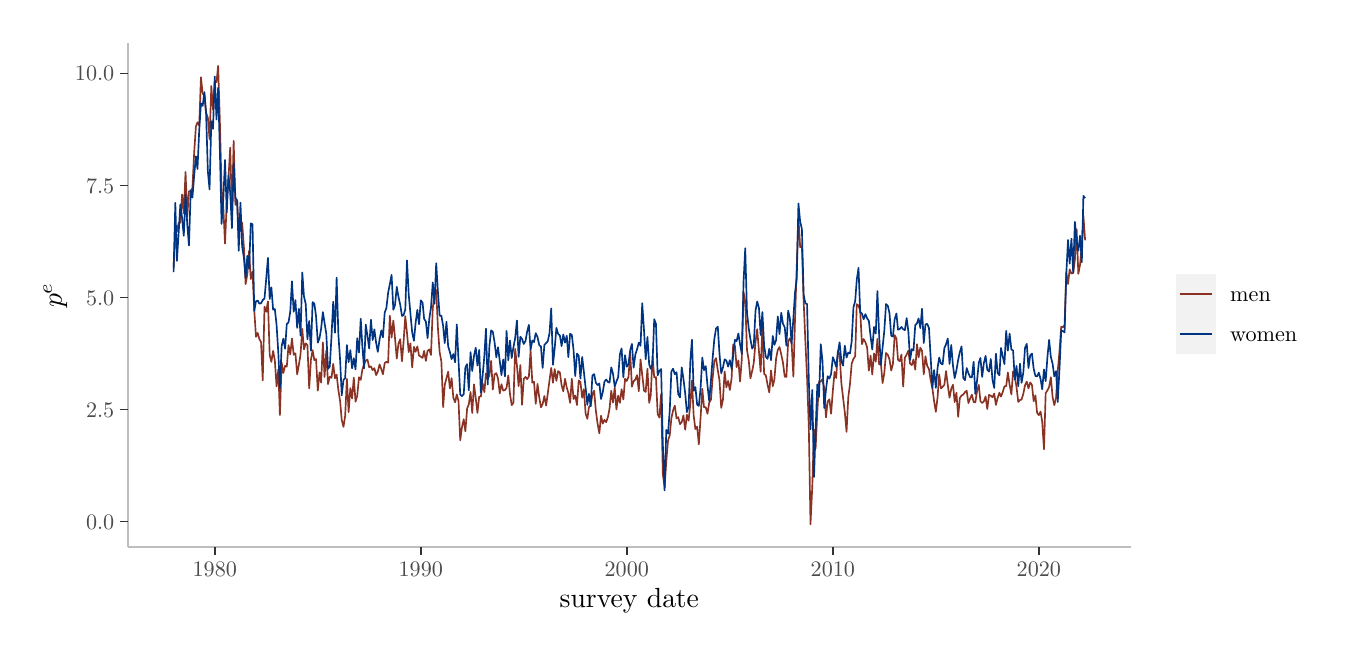
\begin{tikzpicture}[x=1pt,y=1pt]
\definecolor{fillColor}{RGB}{255,255,255}
\path[use as bounding box,fill=fillColor,fill opacity=0.00] (0,0) rectangle (469.75,216.81);
\begin{scope}
\path[clip] (  0.00,  0.00) rectangle (469.75,216.81);
\definecolor{drawColor}{RGB}{255,255,255}
\definecolor{fillColor}{RGB}{255,255,255}

\path[draw=drawColor,line width= 0.6pt,line join=round,line cap=round,fill=fillColor] (  0.00,  0.00) rectangle (469.75,216.81);
\end{scope}
\begin{scope}
\path[clip] ( 36.25, 29.10) rectangle (398.58,211.31);
\definecolor{drawColor}{RGB}{255,255,255}

\path[draw=drawColor,line width= 0.6pt,line join=round] ( 36.25, 38.36) --
	(398.58, 38.36);

\path[draw=drawColor,line width= 0.6pt,line join=round] ( 36.25, 78.84) --
	(398.58, 78.84);

\path[draw=drawColor,line width= 0.6pt,line join=round] ( 36.25,119.33) --
	(398.58,119.33);

\path[draw=drawColor,line width= 0.6pt,line join=round] ( 36.25,159.81) --
	(398.58,159.81);

\path[draw=drawColor,line width= 0.6pt,line join=round] ( 36.25,200.30) --
	(398.58,200.30);

\path[draw=drawColor,line width= 0.6pt,line join=round] ( 67.60, 29.10) --
	( 67.60,211.31);

\path[draw=drawColor,line width= 0.6pt,line join=round] (142.05, 29.10) --
	(142.05,211.31);

\path[draw=drawColor,line width= 0.6pt,line join=round] (216.49, 29.10) --
	(216.49,211.31);

\path[draw=drawColor,line width= 0.6pt,line join=round] (290.95, 29.10) --
	(290.95,211.31);

\path[draw=drawColor,line width= 0.6pt,line join=round] (365.38, 29.10) --
	(365.38,211.31);
\definecolor{drawColor}{RGB}{138,51,36}

\path[draw=drawColor,line width= 0.6pt,line join=round] ( 52.72,130.17) --
	( 53.35,142.05) --
	( 53.92,143.21) --
	( 54.55,146.20) --
	( 55.17,146.36) --
	( 55.80,156.56) --
	( 56.41,149.72) --
	( 57.04,164.69) --
	( 57.67,148.47) --
	( 58.28,157.67) --
	( 58.92,157.81) --
	( 59.53,158.84) --
	( 60.16,171.63) --
	( 60.79,181.10) --
	( 61.36,182.62) --
	( 61.99,181.47) --
	( 62.61,198.90) --
	( 63.24,192.86) --
	( 63.85,192.81) --
	( 64.48,186.03) --
	( 65.11,184.27) --
	( 65.72,176.54) --
	( 66.36,195.73) --
	( 66.97,187.17) --
	( 67.60,197.53) --
	( 68.23,197.10) --
	( 68.82,203.03) --
	( 69.45,182.88) --
	( 70.06,158.84) --
	( 70.70,151.78) --
	( 71.31,138.77) --
	( 71.94,153.64) --
	( 72.57,162.62) --
	( 73.18,173.47) --
	( 73.82,150.34) --
	( 74.43,175.89) --
	( 75.06,152.78) --
	( 75.69,154.00) --
	( 76.26,142.53) --
	( 76.89,144.48) --
	( 77.50,146.30) --
	( 78.14,137.41) --
	( 78.75,124.13) --
	( 79.38,127.79) --
	( 80.01,136.11) --
	( 80.62,125.94) --
	( 81.25,128.63) --
	( 81.87,114.84) --
	( 82.50,105.09) --
	( 83.13,106.48) --
	( 83.70,104.30) --
	( 84.33,103.19) --
	( 84.94, 89.35) --
	( 85.58,115.99) --
	( 86.19,114.18) --
	( 86.82,117.89) --
	( 87.45, 98.62) --
	( 88.06, 96.04) --
	( 88.69,100.01) --
	( 89.31, 96.57) --
	( 89.94, 87.16) --
	( 90.57, 93.32) --
	( 91.14, 76.83) --
	( 91.77, 95.78) --
	( 92.38, 92.03) --
	( 93.02, 94.62) --
	( 93.63, 94.30) --
	( 94.26,102.07) --
	( 94.89, 98.76) --
	( 95.50,104.49) --
	( 96.13, 98.61) --
	( 96.75, 99.11) --
	( 97.38, 91.54) --
	( 98.01, 95.06) --
	( 98.60, 98.80) --
	( 99.23,107.96) --
	( 99.84,100.55) --
	(100.47,102.74) --
	(101.09,102.09) --
	(101.72, 86.46) --
	(102.35, 96.76) --
	(102.96,100.28) --
	(103.59, 96.67) --
	(104.20, 97.06) --
	(104.84, 85.63) --
	(105.47, 92.24) --
	(106.04, 88.56) --
	(106.67,103.08) --
	(107.28, 90.59) --
	(107.91,100.12) --
	(108.53, 88.00) --
	(109.16, 90.73) --
	(109.79, 90.28) --
	(110.40, 95.33) --
	(111.03, 90.12) --
	(111.64, 91.45) --
	(112.28, 85.74) --
	(112.91, 81.80) --
	(113.48, 75.05) --
	(114.11, 72.56) --
	(114.72, 76.50) --
	(115.35, 89.90) --
	(115.97, 77.85) --
	(116.60, 86.54) --
	(117.23, 82.81) --
	(117.84, 90.36) --
	(118.47, 81.66) --
	(119.08, 83.75) --
	(119.72, 90.49) --
	(120.35, 89.52) --
	(120.92, 93.16) --
	(121.55, 95.19) --
	(122.16, 96.54) --
	(122.79, 96.85) --
	(123.40, 94.10) --
	(124.04, 94.40) --
	(124.67, 93.07) --
	(125.28, 93.76) --
	(125.91, 91.26) --
	(126.52, 92.50) --
	(127.16, 95.11) --
	(127.79, 93.40) --
	(128.38, 91.55) --
	(129.01, 95.58) --
	(129.62, 96.10) --
	(130.25, 95.75) --
	(130.86,112.73) --
	(131.50,104.80) --
	(132.13,110.99) --
	(132.74,104.59) --
	(133.37, 97.22) --
	(133.98,102.61) --
	(134.62,104.23) --
	(135.25, 96.26) --
	(135.82,103.21) --
	(136.45,112.50) --
	(137.06,106.57) --
	(137.69, 99.58) --
	(138.30,102.73) --
	(138.94, 94.03) --
	(139.57,101.48) --
	(140.18, 99.70) --
	(140.81,101.64) --
	(141.42, 98.34) --
	(142.05, 97.92) --
	(142.69, 97.46) --
	(143.26, 99.99) --
	(143.89, 96.39) --
	(144.50,100.06) --
	(145.13,100.53) --
	(145.74, 98.54) --
	(146.38,115.43) --
	(147.01,120.68) --
	(147.62,122.04) --
	(148.25,108.12) --
	(148.86, 99.55) --
	(149.49, 96.16) --
	(150.13, 79.69) --
	(150.70, 87.70) --
	(151.33, 90.18) --
	(151.94, 92.48) --
	(152.57, 86.45) --
	(153.18, 90.18) --
	(153.81, 83.13) --
	(154.45, 81.42) --
	(155.06, 84.30) --
	(155.69, 81.74) --
	(156.30, 67.69) --
	(156.93, 72.47) --
	(157.57, 75.32) --
	(158.16, 70.95) --
	(158.79, 79.21) --
	(159.40, 80.73) --
	(160.03, 85.16) --
	(160.64, 77.57) --
	(161.27, 87.93) --
	(161.91, 82.91) --
	(162.52, 77.60) --
	(163.15, 83.48) --
	(163.76, 83.49) --
	(164.39, 88.35) --
	(165.03, 85.11) --
	(165.60, 91.89) --
	(166.23, 89.92) --
	(166.84, 91.17) --
	(167.47, 96.42) --
	(168.08, 86.03) --
	(168.71, 91.56) --
	(169.35, 91.96) --
	(169.96, 90.02) --
	(170.59, 84.66) --
	(171.20, 87.97) --
	(171.83, 85.68) --
	(172.46, 85.88) --
	(173.04, 86.64) --
	(173.67, 91.12) --
	(174.28, 84.45) --
	(174.91, 80.40) --
	(175.52, 81.31) --
	(176.15,100.75) --
	(176.79, 94.72) --
	(177.40, 87.26) --
	(178.03, 94.92) --
	(178.64, 80.53) --
	(179.27, 89.95) --
	(179.90, 90.60) --
	(180.47, 89.78) --
	(181.11, 90.75) --
	(181.72,100.21) --
	(182.35, 88.50) --
	(182.96, 88.86) --
	(183.59, 80.94) --
	(184.23, 88.09) --
	(184.84, 83.31) --
	(185.47, 79.63) --
	(186.08, 80.80) --
	(186.71, 83.71) --
	(187.34, 80.23) --
	(187.93, 84.60) --
	(188.57, 89.42) --
	(189.18, 93.86) --
	(189.81, 88.48) --
	(190.42, 93.45) --
	(191.05, 89.18) --
	(191.68, 92.72) --
	(192.30, 92.24) --
	(192.93, 87.60) --
	(193.54, 85.40) --
	(194.17, 89.95) --
	(194.80, 86.72) --
	(195.37, 84.84) --
	(196.01, 81.24) --
	(196.62, 89.94) --
	(197.25, 82.60) --
	(197.86, 83.90) --
	(198.49, 80.43) --
	(199.12, 89.33) --
	(199.74, 88.76) --
	(200.37, 83.09) --
	(200.98, 86.19) --
	(201.61, 77.32) --
	(202.24, 75.46) --
	(202.81, 79.67) --
	(203.45, 80.44) --
	(204.06, 84.29) --
	(204.69, 85.64) --
	(205.30, 78.46) --
	(205.93, 73.76) --
	(206.56, 70.22) --
	(207.18, 76.58) --
	(207.81, 73.74) --
	(208.42, 75.11) --
	(209.05, 74.25) --
	(209.68, 76.12) --
	(210.25, 79.10) --
	(210.88, 85.59) --
	(211.50, 81.33) --
	(212.13, 86.79) --
	(212.74, 78.84) --
	(213.37, 83.89) --
	(214.00, 81.27) --
	(214.61, 86.14) --
	(215.25, 82.46) --
	(215.86, 89.96) --
	(216.49, 89.14) --
	(217.12, 90.69) --
	(217.71, 99.53) --
	(218.34, 87.08) --
	(218.96, 89.06) --
	(219.59, 89.68) --
	(220.20, 91.27) --
	(220.83, 85.44) --
	(221.46, 96.92) --
	(222.07, 91.32) --
	(222.71, 85.65) --
	(223.32, 85.22) --
	(223.95, 93.56) --
	(224.58, 81.25) --
	(225.15, 83.96) --
	(225.78, 98.12) --
	(226.40, 90.47) --
	(227.03, 90.54) --
	(227.64, 77.21) --
	(228.27, 75.91) --
	(228.90, 84.42) --
	(229.51, 55.50) --
	(230.15, 50.78) --
	(230.76, 60.12) --
	(231.39, 67.61) --
	(232.02, 69.58) --
	(232.59, 75.61) --
	(233.22, 78.52) --
	(233.84, 80.24) --
	(234.47, 75.63) --
	(235.08, 76.04) --
	(235.71, 73.52) --
	(236.34, 74.31) --
	(236.95, 76.70) --
	(237.59, 71.53) --
	(238.20, 76.93) --
	(238.83, 74.79) --
	(239.46, 81.14) --
	(240.03, 89.34) --
	(240.66, 76.60) --
	(241.27, 71.77) --
	(241.91, 72.64) --
	(242.52, 66.25) --
	(243.15, 75.86) --
	(243.78, 86.31) --
	(244.39, 79.69) --
	(245.02, 79.66) --
	(245.64, 77.31) --
	(246.27, 81.33) --
	(246.90, 82.40) --
	(247.49, 89.97) --
	(248.12, 96.36) --
	(248.73, 97.39) --
	(249.37, 93.05) --
	(249.98, 89.42) --
	(250.61, 79.41) --
	(251.24, 82.43) --
	(251.85, 92.58) --
	(252.48, 86.87) --
	(253.10, 89.16) --
	(253.73, 85.89) --
	(254.36, 90.11) --
	(254.93,102.34) --
	(255.56,101.85) --
	(256.17, 94.15) --
	(256.81, 96.59) --
	(257.42, 88.95) --
	(258.05, 97.11) --
	(258.68,121.22) --
	(259.29,118.02) --
	(259.92,100.29) --
	(260.54, 96.66) --
	(261.17, 90.09) --
	(261.80, 92.78) --
	(262.37, 95.68) --
	(263.00,103.21) --
	(263.61,107.87) --
	(264.25, 99.79) --
	(264.86, 92.47) --
	(265.49,109.31) --
	(266.12, 91.71) --
	(266.73, 91.17) --
	(267.36, 87.76) --
	(267.98, 85.02) --
	(268.61, 92.91) --
	(269.24, 87.25) --
	(269.81, 89.60) --
	(270.44, 97.25) --
	(271.05,100.38) --
	(271.68,101.41) --
	(272.30, 98.78) --
	(272.93, 95.70) --
	(273.56, 90.68) --
	(274.17, 90.61) --
	(274.80,103.37) --
	(275.41,104.57) --
	(276.05,102.80) --
	(276.68, 90.69) --
	(277.27,111.05) --
	(277.90,130.66) --
	(278.51,148.10) --
	(279.14,137.46) --
	(279.76,137.94) --
	(280.39,118.20) --
	(281.02,103.44) --
	(281.63, 90.32) --
	(282.26, 72.60) --
	(282.87, 37.38) --
	(283.51, 50.85) --
	(284.14, 71.60) --
	(284.71, 64.64) --
	(285.34, 77.98) --
	(285.95, 88.73) --
	(286.58, 88.97) --
	(287.20, 89.82) --
	(287.83, 86.54) --
	(288.46, 75.99) --
	(289.07, 81.73) --
	(289.70, 82.50) --
	(290.31, 77.30) --
	(290.95, 85.68) --
	(291.58, 92.45) --
	(292.15, 90.22) --
	(292.78, 99.97) --
	(293.39, 98.87) --
	(294.02, 88.43) --
	(294.63, 83.17) --
	(295.27, 77.82) --
	(295.90, 70.74) --
	(296.51, 83.09) --
	(297.14, 88.04) --
	(297.75, 95.37) --
	(298.39, 97.14) --
	(299.02, 98.06) --
	(299.59,116.88) --
	(300.22,116.40) --
	(300.83,114.52) --
	(301.46,102.45) --
	(302.07,104.30) --
	(302.71,103.13) --
	(303.34,101.21) --
	(303.95, 92.86) --
	(304.58, 98.30) --
	(305.19, 91.50) --
	(305.82, 99.08) --
	(306.46, 96.10) --
	(307.05,104.38) --
	(307.68, 95.07) --
	(308.29, 95.62) --
	(308.92, 88.40) --
	(309.53, 91.92) --
	(310.17, 99.26) --
	(310.80, 98.62) --
	(311.41, 96.97) --
	(312.04, 92.91) --
	(312.65, 95.29) --
	(313.28,105.70) --
	(313.92,104.43) --
	(314.49, 96.78) --
	(315.12, 96.30) --
	(315.73, 98.68) --
	(316.36, 87.09) --
	(316.97, 97.55) --
	(317.61, 98.66) --
	(318.24,100.09) --
	(318.85, 95.39) --
	(319.48, 94.87) --
	(320.09, 96.93) --
	(320.72, 93.24) --
	(321.36,102.45) --
	(321.93, 97.67) --
	(322.56,101.16) --
	(323.17,100.01) --
	(323.80, 91.55) --
	(324.41, 98.06) --
	(325.04, 94.60) --
	(325.68, 93.46) --
	(326.29, 89.43) --
	(326.92, 86.47) --
	(327.53, 81.83) --
	(328.16, 77.97) --
	(328.80, 83.35) --
	(329.37, 91.52) --
	(330.00, 86.46) --
	(330.61, 87.05) --
	(331.24, 87.72) --
	(331.85, 92.71) --
	(332.48, 87.64) --
	(333.12, 83.11) --
	(333.73, 86.35) --
	(334.36, 87.75) --
	(334.97, 81.52) --
	(335.60, 84.88) --
	(336.23, 76.18) --
	(336.83, 82.96) --
	(337.46, 83.90) --
	(338.07, 84.23) --
	(338.70, 85.13) --
	(339.31, 85.63) --
	(339.94, 81.14) --
	(340.58, 82.87) --
	(341.19, 84.19) --
	(341.82, 81.53) --
	(342.43, 81.43) --
	(343.06, 85.53) --
	(343.69, 87.71) --
	(344.27, 81.84) --
	(344.90, 81.20) --
	(345.51, 81.76) --
	(346.14, 83.53) --
	(346.75, 78.98) --
	(347.38, 84.11) --
	(348.02, 83.83) --
	(348.63, 83.25) --
	(349.26, 84.59) --
	(349.87, 80.49) --
	(350.50, 83.03) --
	(351.13, 84.91) --
	(351.70, 83.48) --
	(352.34, 85.15) --
	(352.95, 87.21) --
	(353.58, 87.27) --
	(354.19, 92.21) --
	(354.82, 87.78) --
	(355.46, 84.28) --
	(356.07, 92.55) --
	(356.70, 90.61) --
	(357.31, 86.98) --
	(357.94, 81.57) --
	(358.57, 82.27) --
	(359.14, 82.41) --
	(359.78, 84.57) --
	(360.39, 87.59) --
	(361.02, 88.88) --
	(361.63, 86.48) --
	(362.26, 88.61) --
	(362.89, 87.72) --
	(363.51, 81.82) --
	(364.14, 83.96) --
	(364.75, 77.65) --
	(365.38, 76.78) --
	(366.01, 78.09) --
	(366.60, 74.35) --
	(367.24, 64.44) --
	(367.85, 84.73) --
	(368.48, 85.74) --
	(369.09, 86.99) --
	(369.72, 90.50) --
	(370.35, 83.33) --
	(370.97, 80.41) --
	(371.60, 82.99) --
	(372.21, 92.76) --
	(372.84, 99.86) --
	(373.47,108.83) --
	(374.04,108.51) --
	(374.68,109.35) --
	(375.29,128.50) --
	(375.92,124.18) --
	(376.53,129.44) --
	(377.16,127.99) --
	(377.79,128.03) --
	(378.41,132.97) --
	(379.04,143.98) --
	(379.65,127.86) --
	(380.28,131.19) --
	(380.91,138.32) --
	(381.48,148.77) --
	(382.11,139.98);
\definecolor{drawColor}{RGB}{0,51,128}

\path[draw=drawColor,line width= 0.6pt,line join=round] ( 52.72,128.46) --
	( 53.35,153.49) --
	( 53.92,132.53) --
	( 54.55,142.51) --
	( 55.17,152.95) --
	( 55.80,147.99) --
	( 56.41,141.60) --
	( 57.04,156.50) --
	( 57.67,145.61) --
	( 58.28,138.11) --
	( 58.92,158.04) --
	( 59.53,155.45) --
	( 60.16,163.34) --
	( 60.79,170.33) --
	( 61.36,165.74) --
	( 61.99,179.85) --
	( 62.61,189.43) --
	( 63.24,188.57) --
	( 63.85,193.55) --
	( 64.48,185.55) --
	( 65.11,164.88) --
	( 65.72,158.36) --
	( 66.36,183.02) --
	( 66.97,180.23) --
	( 67.60,199.21) --
	( 68.23,183.59) --
	( 68.82,195.08) --
	( 69.45,172.39) --
	( 70.06,145.89) --
	( 70.70,154.99) --
	( 71.31,169.02) --
	( 71.94,150.06) --
	( 72.57,163.47) --
	( 73.18,157.20) --
	( 73.82,144.37) --
	( 74.43,167.91) --
	( 75.06,155.37) --
	( 75.69,154.40) --
	( 76.26,136.21) --
	( 76.89,153.59) --
	( 77.50,137.67) --
	( 78.14,133.73) --
	( 78.75,126.38) --
	( 79.38,134.39) --
	( 80.01,129.76) --
	( 80.62,146.08) --
	( 81.25,145.75) --
	( 81.87,114.41) --
	( 82.50,117.94) --
	( 83.13,118.20) --
	( 83.70,117.09) --
	( 84.33,117.24) --
	( 84.94,118.37) --
	( 85.58,119.01) --
	( 86.19,125.96) --
	( 86.82,133.62) --
	( 87.45,118.76) --
	( 88.06,122.97) --
	( 88.69,114.89) --
	( 89.31,115.15) --
	( 89.94,109.38) --
	( 90.57, 99.28) --
	( 91.14, 86.61) --
	( 91.77,101.72) --
	( 92.38,104.45) --
	( 93.02,100.78) --
	( 93.63,109.75) --
	( 94.26,110.31) --
	( 94.89,114.23) --
	( 95.50,125.15) --
	( 96.13,114.13) --
	( 96.75,118.35) --
	( 97.38,108.32) --
	( 98.01,115.20) --
	( 98.60,105.54) --
	( 99.23,128.37) --
	( 99.84,119.70) --
	(100.47,116.97) --
	(101.09,104.21) --
	(101.72,110.81) --
	(102.35,100.10) --
	(102.96,117.64) --
	(103.59,117.09) --
	(104.20,112.56) --
	(104.84,102.99) --
	(105.47,104.65) --
	(106.04,108.06) --
	(106.67,114.05) --
	(107.28,110.11) --
	(107.91,106.17) --
	(108.53, 93.52) --
	(109.16, 94.34) --
	(109.79,105.32) --
	(110.40,117.77) --
	(111.03,106.56) --
	(111.64,126.49) --
	(112.28,105.83) --
	(112.91, 96.55) --
	(113.48, 83.94) --
	(114.11, 89.48) --
	(114.72, 90.18) --
	(115.35,102.12) --
	(115.97, 95.96) --
	(116.60,100.28) --
	(117.23, 93.68) --
	(117.84, 97.38) --
	(118.47, 93.33) --
	(119.08,104.58) --
	(119.72, 99.42) --
	(120.35,111.63) --
	(120.92,101.90) --
	(121.55, 93.68) --
	(122.16,109.51) --
	(122.79,105.45) --
	(123.40,100.86) --
	(124.04,111.28) --
	(124.67,103.92) --
	(125.28,107.77) --
	(125.91,102.94) --
	(126.52, 99.67) --
	(127.16,104.16) --
	(127.79,107.43) --
	(128.38,104.90) --
	(129.01,113.82) --
	(129.62,115.51) --
	(130.25,121.01) --
	(130.86,124.07) --
	(131.50,127.46) --
	(132.13,114.86) --
	(132.74,116.63) --
	(133.37,123.15) --
	(133.98,119.59) --
	(134.62,116.68) --
	(135.25,112.64) --
	(135.82,112.88) --
	(136.45,114.97) --
	(137.06,132.73) --
	(137.69,120.42) --
	(138.30,113.58) --
	(138.94,106.70) --
	(139.57,103.67) --
	(140.18,110.10) --
	(140.81,114.82) --
	(141.42,109.67) --
	(142.05,118.29) --
	(142.69,117.45) --
	(143.26,111.59) --
	(143.89,110.60) --
	(144.50,104.63) --
	(145.13,111.66) --
	(145.74,115.68) --
	(146.38,124.70) --
	(147.01,117.05) --
	(147.62,131.71) --
	(148.25,121.24) --
	(148.86,112.74) --
	(149.49,112.73) --
	(150.13,108.98) --
	(150.70,102.82) --
	(151.33,110.55) --
	(151.94,101.66) --
	(152.57, 99.58) --
	(153.18, 97.04) --
	(153.81, 98.88) --
	(154.45, 95.85) --
	(155.06,109.61) --
	(155.69, 96.43) --
	(156.30, 84.25) --
	(156.93, 83.67) --
	(157.57, 84.38) --
	(158.16, 94.06) --
	(158.79, 95.23) --
	(159.40, 85.75) --
	(160.03, 99.58) --
	(160.64, 92.75) --
	(161.27, 98.18) --
	(161.91,101.18) --
	(162.52, 94.71) --
	(163.15,100.37) --
	(163.76, 84.94) --
	(164.39, 90.90) --
	(165.03, 98.35) --
	(165.60,108.05) --
	(166.23, 87.85) --
	(166.84,101.73) --
	(167.47,107.43) --
	(168.08,106.92) --
	(168.71,103.13) --
	(169.35, 97.66) --
	(169.96,101.33) --
	(170.59, 96.38) --
	(171.20, 91.26) --
	(171.83, 96.89) --
	(172.46, 90.79) --
	(173.04,107.21) --
	(173.67, 96.63) --
	(174.28,103.75) --
	(174.91, 97.45) --
	(175.52,101.25) --
	(176.15,104.66) --
	(176.79,110.98) --
	(177.40, 97.86) --
	(178.03,105.14) --
	(178.64,104.32) --
	(179.27,102.50) --
	(179.90,103.64) --
	(180.47,106.96) --
	(181.11,109.42) --
	(181.72,100.42) --
	(182.35,103.77) --
	(182.96,103.20) --
	(183.59,106.41) --
	(184.23,105.00) --
	(184.84,102.16) --
	(185.47,101.57) --
	(186.08, 93.85) --
	(186.71,102.15) --
	(187.34,102.86) --
	(187.93,103.46) --
	(188.57,106.43) --
	(189.18,115.39) --
	(189.81, 95.00) --
	(190.42,100.81) --
	(191.05,108.33) --
	(191.68,106.15) --
	(192.30,105.63) --
	(192.93,101.76) --
	(193.54,105.95) --
	(194.17,103.00) --
	(194.80,105.49) --
	(195.37, 97.78) --
	(196.01,106.19) --
	(196.62,105.80) --
	(197.25,100.34) --
	(197.86, 90.95) --
	(198.49, 99.05) --
	(199.12, 98.23) --
	(199.74, 89.98) --
	(200.37, 97.83) --
	(200.98, 92.46) --
	(201.61, 86.69) --
	(202.24, 80.52) --
	(202.81, 84.49) --
	(203.45, 79.97) --
	(204.06, 91.06) --
	(204.69, 91.63) --
	(205.30, 88.53) --
	(205.93, 87.69) --
	(206.56, 88.24) --
	(207.18, 82.63) --
	(207.81, 85.12) --
	(208.42, 88.88) --
	(209.05, 89.68) --
	(209.68, 88.80) --
	(210.25, 88.52) --
	(210.88, 94.05) --
	(211.50, 91.79) --
	(212.13, 87.15) --
	(212.74, 88.96) --
	(213.37, 90.52) --
	(214.00, 98.72) --
	(214.61,100.93) --
	(215.25, 90.48) --
	(215.86, 98.45) --
	(216.49, 94.29) --
	(217.12, 95.30) --
	(217.71,100.21) --
	(218.34,102.53) --
	(218.96, 93.94) --
	(219.59, 98.73) --
	(220.20,100.58) --
	(220.83,103.00) --
	(221.46,101.88) --
	(222.07,117.25) --
	(222.71,107.43) --
	(223.32, 97.01) --
	(223.95,105.03) --
	(224.58, 95.11) --
	(225.15, 93.50) --
	(225.78, 95.37) --
	(226.40,111.47) --
	(227.03,109.76) --
	(227.64, 91.20) --
	(228.27, 92.79) --
	(228.90, 93.46) --
	(229.51, 66.26) --
	(230.15, 49.58) --
	(230.76, 71.47) --
	(231.39, 70.08) --
	(232.02, 78.63) --
	(232.59, 92.54) --
	(233.22, 93.58) --
	(233.84, 91.60) --
	(234.47, 92.31) --
	(235.08, 84.37) --
	(235.71, 83.19) --
	(236.34, 94.06) --
	(236.95, 89.96) --
	(237.59, 84.69) --
	(238.20, 77.86) --
	(238.83, 79.97) --
	(239.46, 96.44) --
	(240.03,104.05) --
	(240.66, 85.62) --
	(241.27, 86.94) --
	(241.91, 80.56) --
	(242.52, 80.13) --
	(243.15, 86.41) --
	(243.78, 97.60) --
	(244.39, 93.05) --
	(245.02, 94.50) --
	(245.64, 87.57) --
	(246.27, 81.90) --
	(246.90, 89.39) --
	(247.49, 97.15) --
	(248.12,104.26) --
	(248.73,108.12) --
	(249.37,108.75) --
	(249.98, 99.03) --
	(250.61, 91.93) --
	(251.24, 94.02) --
	(251.85, 96.97) --
	(252.48, 96.49) --
	(253.10, 94.36) --
	(253.73, 96.68) --
	(254.36, 93.63) --
	(254.93, 98.17) --
	(255.56,103.99) --
	(256.17,103.56) --
	(256.81,106.29) --
	(257.42,102.31) --
	(258.05, 98.98) --
	(258.68,125.00) --
	(259.29,137.10) --
	(259.92,113.93) --
	(260.54,108.25) --
	(261.17,104.18) --
	(261.80,100.82) --
	(262.37,101.83) --
	(263.00,114.53) --
	(263.61,117.88) --
	(264.25,115.45) --
	(264.86,105.75) --
	(265.49,114.04) --
	(266.12,101.81) --
	(266.73, 97.89) --
	(267.36, 97.12) --
	(267.98,100.78) --
	(268.61, 96.66) --
	(269.24,105.42) --
	(269.81,102.20) --
	(270.44,103.89) --
	(271.05,112.47) --
	(271.68,106.08) --
	(272.30,113.77) --
	(272.93,109.81) --
	(273.56,108.51) --
	(274.17,101.88) --
	(274.80,114.58) --
	(275.41,111.82) --
	(276.05,102.52) --
	(276.68,111.74) --
	(277.27,121.02) --
	(277.90,126.13) --
	(278.51,153.30) --
	(279.14,146.67) --
	(279.76,144.12) --
	(280.39,120.28) --
	(281.02,117.20) --
	(281.63,116.93) --
	(282.26, 89.48) --
	(282.87, 71.65) --
	(283.51, 85.93) --
	(284.14, 54.41) --
	(284.71, 71.17) --
	(285.34, 87.93) --
	(285.95, 83.33) --
	(286.58,102.42) --
	(287.20, 96.40) --
	(287.83, 79.34) --
	(288.46, 85.95) --
	(289.07, 90.85) --
	(289.70, 90.02) --
	(290.31, 91.67) --
	(290.95, 97.71) --
	(291.58, 96.16) --
	(292.15, 94.23) --
	(292.78, 99.41) --
	(293.39,103.13) --
	(294.02, 96.38) --
	(294.63, 94.68) --
	(295.27,101.92) --
	(295.90, 97.63) --
	(296.51, 99.39) --
	(297.14, 99.07) --
	(297.75,103.41) --
	(298.39,115.74) --
	(299.02,118.02) --
	(299.59,125.66) --
	(300.22,130.02) --
	(300.83,113.93) --
	(301.46,113.52) --
	(302.07,111.46) --
	(302.71,113.31) --
	(303.34,111.75) --
	(303.95,110.91) --
	(304.58,105.26) --
	(305.19,100.53) --
	(305.82,108.64) --
	(306.46,106.29) --
	(307.05,121.63) --
	(307.68,105.48) --
	(308.29, 95.04) --
	(308.92,101.25) --
	(309.53,107.18) --
	(310.17,116.95) --
	(310.80,116.33) --
	(311.41,113.68) --
	(312.04,105.49) --
	(312.65,105.18) --
	(313.28,111.44) --
	(313.92,113.51) --
	(314.49,107.68) --
	(315.12,107.95) --
	(315.73,108.66) --
	(316.36,107.85) --
	(316.97,107.51) --
	(317.61,111.86) --
	(318.24,106.98) --
	(318.85, 96.74) --
	(319.48,100.63) --
	(320.09,100.16) --
	(320.72,109.30) --
	(321.36,109.99) --
	(321.93,111.73) --
	(322.56,108.27) --
	(323.17,115.22) --
	(323.80,102.89) --
	(324.41,109.56) --
	(325.04,109.79) --
	(325.68,108.26) --
	(326.29, 97.68) --
	(326.92, 86.58) --
	(327.53, 93.10) --
	(328.16, 86.67) --
	(328.80, 93.89) --
	(329.37, 97.62) --
	(330.00, 95.45) --
	(330.61, 95.13) --
	(331.24,101.00) --
	(331.85,102.43) --
	(332.48,104.47) --
	(333.12, 95.29) --
	(333.73,102.12) --
	(334.36, 94.65) --
	(334.97, 90.18) --
	(335.60, 93.01) --
	(336.23, 96.79) --
	(336.83, 99.53) --
	(337.46,101.64) --
	(338.07, 90.25) --
	(338.70, 89.43) --
	(339.31, 93.83) --
	(339.94, 91.94) --
	(340.58, 90.50) --
	(341.19, 90.47) --
	(341.82, 96.09) --
	(342.43, 84.45) --
	(343.06, 89.32) --
	(343.69, 95.68) --
	(344.27, 97.46) --
	(344.90, 90.60) --
	(345.51, 95.58) --
	(346.14, 98.19) --
	(346.75, 93.23) --
	(347.38, 92.53) --
	(348.02, 97.09) --
	(348.63, 89.57) --
	(349.26, 86.62) --
	(349.87, 99.00) --
	(350.50, 92.02) --
	(351.13, 91.20) --
	(351.70,101.08) --
	(352.34, 98.09) --
	(352.95, 95.23) --
	(353.58,107.26) --
	(354.19,100.12) --
	(354.82,106.24) --
	(355.46,100.47) --
	(356.07,100.18) --
	(356.70, 89.65) --
	(357.31, 94.54) --
	(357.94, 87.23) --
	(358.57, 95.36) --
	(359.14, 88.49) --
	(359.78, 92.28) --
	(360.39,101.12) --
	(361.02,102.55) --
	(361.63, 93.81) --
	(362.26, 98.42) --
	(362.89, 99.03) --
	(363.51, 93.58) --
	(364.14, 90.95) --
	(364.75, 90.80) --
	(365.38, 92.15) --
	(366.01, 89.85) --
	(366.60, 86.13) --
	(367.24, 93.29) --
	(367.85, 89.07) --
	(368.48, 97.71) --
	(369.09,104.00) --
	(369.72, 97.83) --
	(370.35, 95.37) --
	(370.97, 90.80) --
	(371.60, 92.72) --
	(372.21, 81.57) --
	(372.84, 93.42) --
	(373.47,107.35) --
	(374.04,107.18) --
	(374.68,106.66) --
	(375.29,127.52) --
	(375.92,140.09) --
	(376.53,131.56) --
	(377.16,140.57) --
	(377.79,128.38) --
	(378.41,146.62) --
	(379.04,139.55) --
	(379.65,136.23) --
	(380.28,141.63) --
	(380.91,132.03) --
	(381.48,156.01) --
	(382.11,155.24);
\end{scope}
\begin{scope}
\path[clip] (  0.00,  0.00) rectangle (469.75,216.81);
\definecolor{drawColor}{RGB}{190,190,190}

\path[draw=drawColor,line width= 0.6pt,line join=round] ( 36.25, 29.10) --
	( 36.25,211.31);
\end{scope}
\begin{scope}
\path[clip] (  0.00,  0.00) rectangle (469.75,216.81);
\definecolor{drawColor}{gray}{0.30}

\node[text=drawColor,anchor=base east,inner sep=0pt, outer sep=0pt, scale=  0.80] at ( 31.30, 35.60) {0.0};

\node[text=drawColor,anchor=base east,inner sep=0pt, outer sep=0pt, scale=  0.80] at ( 31.30, 76.09) {2.5};

\node[text=drawColor,anchor=base east,inner sep=0pt, outer sep=0pt, scale=  0.80] at ( 31.30,116.57) {5.0};

\node[text=drawColor,anchor=base east,inner sep=0pt, outer sep=0pt, scale=  0.80] at ( 31.30,157.06) {7.5};

\node[text=drawColor,anchor=base east,inner sep=0pt, outer sep=0pt, scale=  0.80] at ( 31.30,197.55) {10.0};
\end{scope}
\begin{scope}
\path[clip] (  0.00,  0.00) rectangle (469.75,216.81);
\definecolor{drawColor}{gray}{0.20}

\path[draw=drawColor,line width= 0.6pt,line join=round] ( 33.50, 38.36) --
	( 36.25, 38.36);

\path[draw=drawColor,line width= 0.6pt,line join=round] ( 33.50, 78.84) --
	( 36.25, 78.84);

\path[draw=drawColor,line width= 0.6pt,line join=round] ( 33.50,119.33) --
	( 36.25,119.33);

\path[draw=drawColor,line width= 0.6pt,line join=round] ( 33.50,159.81) --
	( 36.25,159.81);

\path[draw=drawColor,line width= 0.6pt,line join=round] ( 33.50,200.30) --
	( 36.25,200.30);
\end{scope}
\begin{scope}
\path[clip] (  0.00,  0.00) rectangle (469.75,216.81);
\definecolor{drawColor}{RGB}{190,190,190}

\path[draw=drawColor,line width= 0.6pt,line join=round] ( 36.25, 29.10) --
	(398.58, 29.10);
\end{scope}
\begin{scope}
\path[clip] (  0.00,  0.00) rectangle (469.75,216.81);
\definecolor{drawColor}{gray}{0.20}

\path[draw=drawColor,line width= 0.6pt,line join=round] ( 67.60, 26.35) --
	( 67.60, 29.10);

\path[draw=drawColor,line width= 0.6pt,line join=round] (142.05, 26.35) --
	(142.05, 29.10);

\path[draw=drawColor,line width= 0.6pt,line join=round] (216.49, 26.35) --
	(216.49, 29.10);

\path[draw=drawColor,line width= 0.6pt,line join=round] (290.95, 26.35) --
	(290.95, 29.10);

\path[draw=drawColor,line width= 0.6pt,line join=round] (365.38, 26.35) --
	(365.38, 29.10);
\end{scope}
\begin{scope}
\path[clip] (  0.00,  0.00) rectangle (469.75,216.81);
\definecolor{drawColor}{gray}{0.30}

\node[text=drawColor,anchor=base,inner sep=0pt, outer sep=0pt, scale=  0.80] at ( 67.60, 18.64) {1980};

\node[text=drawColor,anchor=base,inner sep=0pt, outer sep=0pt, scale=  0.80] at (142.05, 18.64) {1990};

\node[text=drawColor,anchor=base,inner sep=0pt, outer sep=0pt, scale=  0.80] at (216.49, 18.64) {2000};

\node[text=drawColor,anchor=base,inner sep=0pt, outer sep=0pt, scale=  0.80] at (290.95, 18.64) {2010};

\node[text=drawColor,anchor=base,inner sep=0pt, outer sep=0pt, scale=  0.80] at (365.38, 18.64) {2020};
\end{scope}
\begin{scope}
\path[clip] (  0.00,  0.00) rectangle (469.75,216.81);
\definecolor{drawColor}{RGB}{0,0,0}

\node[text=drawColor,anchor=base,inner sep=0pt, outer sep=0pt, scale=  1.00] at (217.42,  7.44) {survey date};
\end{scope}
\begin{scope}
\path[clip] (  0.00,  0.00) rectangle (469.75,216.81);
\definecolor{drawColor}{RGB}{0,0,0}

\node[text=drawColor,rotate= 90.00,anchor=base,inner sep=0pt, outer sep=0pt, scale=  1.00] at ( 12.39,120.20) {$p^e$};
\end{scope}
\begin{scope}
\path[clip] (  0.00,  0.00) rectangle (469.75,216.81);
\definecolor{fillColor}{RGB}{255,255,255}

\path[fill=fillColor] (409.58, 93.33) rectangle (464.25,147.07);
\end{scope}
\begin{scope}
\path[clip] (  0.00,  0.00) rectangle (469.75,216.81);
\definecolor{drawColor}{RGB}{0,0,0}

\node[text=drawColor,anchor=base west,inner sep=0pt, outer sep=0pt, scale=  1.00] at (415.08,133.71) { };
\end{scope}
\begin{scope}
\path[clip] (  0.00,  0.00) rectangle (469.75,216.81);
\definecolor{fillColor}{gray}{0.95}

\path[fill=fillColor] (415.08,113.29) rectangle (429.54,127.74);
\end{scope}
\begin{scope}
\path[clip] (  0.00,  0.00) rectangle (469.75,216.81);
\definecolor{drawColor}{RGB}{138,51,36}

\path[draw=drawColor,line width= 0.6pt,line join=round] (416.53,120.51) -- (428.09,120.51);
\end{scope}
\begin{scope}
\path[clip] (  0.00,  0.00) rectangle (469.75,216.81);
\definecolor{fillColor}{gray}{0.95}

\path[fill=fillColor] (415.08, 98.83) rectangle (429.54,113.29);
\end{scope}
\begin{scope}
\path[clip] (  0.00,  0.00) rectangle (469.75,216.81);
\definecolor{drawColor}{RGB}{0,51,128}

\path[draw=drawColor,line width= 0.6pt,line join=round] (416.53,106.06) -- (428.09,106.06);
\end{scope}
\begin{scope}
\path[clip] (  0.00,  0.00) rectangle (469.75,216.81);
\definecolor{drawColor}{RGB}{0,0,0}

\node[text=drawColor,anchor=base west,inner sep=0pt, outer sep=0pt, scale=  0.80] at (434.54,117.76) {men};
\end{scope}
\begin{scope}
\path[clip] (  0.00,  0.00) rectangle (469.75,216.81);
\definecolor{drawColor}{RGB}{0,0,0}

\node[text=drawColor,anchor=base west,inner sep=0pt, outer sep=0pt, scale=  0.80] at (434.54,103.31) {women};
\end{scope}
\end{tikzpicture}

\caption{Inflation expectations: men/women}
\end{subfigure}
\vfill
\begin{subfigure}[t]{0.75\textwidth}
\centering
% Created by tikzDevice version 0.12.6 on 2024-07-18 16:30:20
% !TEX encoding = UTF-8 Unicode
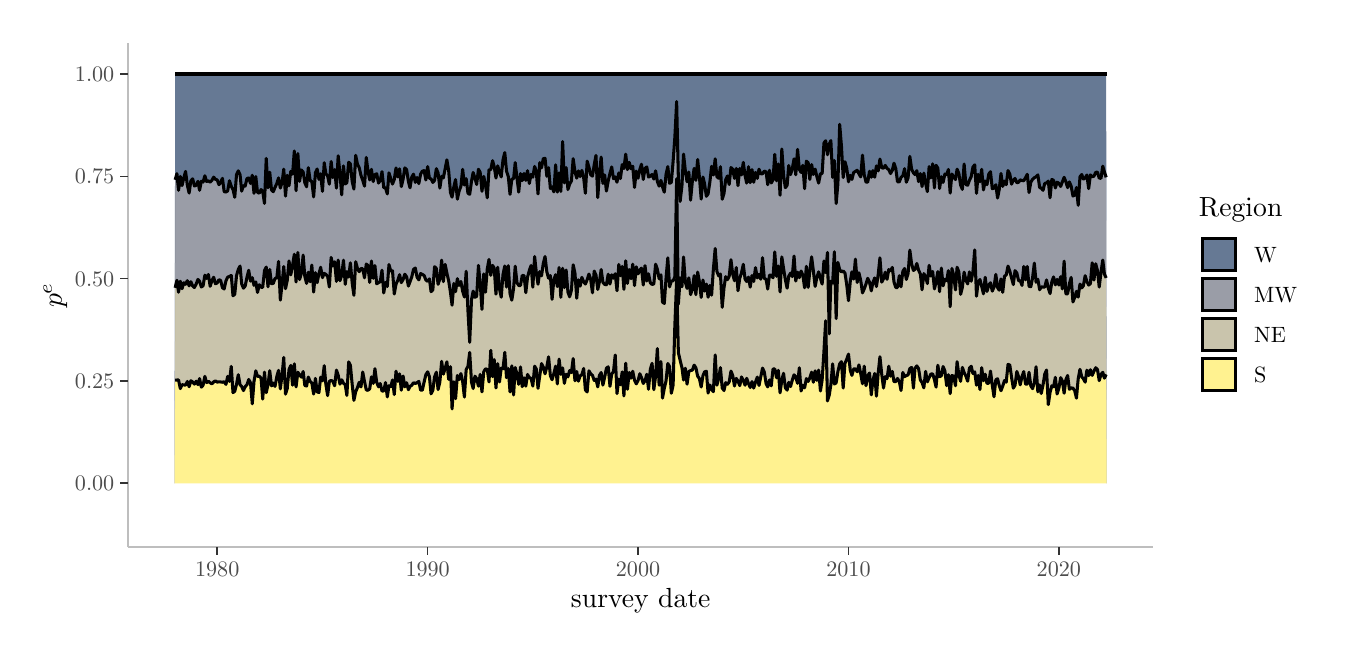
\begin{tikzpicture}[x=1pt,y=1pt]
\definecolor{fillColor}{RGB}{255,255,255}
\path[use as bounding box,fill=fillColor,fill opacity=0.00] (0,0) rectangle (469.75,216.81);
\begin{scope}
\path[clip] (  0.00,  0.00) rectangle (469.75,216.81);
\definecolor{drawColor}{RGB}{255,255,255}
\definecolor{fillColor}{RGB}{255,255,255}

\path[draw=drawColor,line width= 0.6pt,line join=round,line cap=round,fill=fillColor] (  0.00,  0.00) rectangle (469.76,216.81);
\end{scope}
\begin{scope}
\path[clip] ( 36.25, 29.10) rectangle (406.75,211.31);
\definecolor{drawColor}{RGB}{255,255,255}

\path[draw=drawColor,line width= 0.6pt,line join=round] ( 36.25, 52.17) --
	(406.75, 52.17);

\path[draw=drawColor,line width= 0.6pt,line join=round] ( 36.25, 89.14) --
	(406.75, 89.14);

\path[draw=drawColor,line width= 0.6pt,line join=round] ( 36.25,126.12) --
	(406.75,126.12);

\path[draw=drawColor,line width= 0.6pt,line join=round] ( 36.25,163.09) --
	(406.75,163.09);

\path[draw=drawColor,line width= 0.6pt,line join=round] ( 36.25,200.07) --
	(406.75,200.07);

\path[draw=drawColor,line width= 0.6pt,line join=round] ( 68.48, 29.10) --
	( 68.48,211.31);

\path[draw=drawColor,line width= 0.6pt,line join=round] (144.53, 29.10) --
	(144.53,211.31);

\path[draw=drawColor,line width= 0.6pt,line join=round] (220.55, 29.10) --
	(220.55,211.31);

\path[draw=drawColor,line width= 0.6pt,line join=round] (296.60, 29.10) --
	(296.60,211.31);

\path[draw=drawColor,line width= 0.6pt,line join=round] (372.62, 29.10) --
	(372.62,211.31);
\definecolor{fillColor}{RGB}{0,32,77}

\path[fill=fillColor,fill opacity=0.60] ( 53.29,200.07) --
	( 53.48,200.07) --
	( 53.74,200.07) --
	( 53.93,200.07) --
	( 54.12,200.07) --
	( 54.32,200.07) --
	( 54.51,200.07) --
	( 54.71,200.07) --
	( 54.96,200.07) --
	( 55.16,200.07) --
	( 55.35,200.07) --
	( 55.59,200.07) --
	( 55.78,200.07) --
	( 55.98,200.07) --
	( 56.23,200.07) --
	( 56.43,200.07) --
	( 56.62,200.07) --
	( 56.86,200.07) --
	( 57.05,200.07) --
	( 57.25,200.07) --
	( 57.50,200.07) --
	( 57.70,200.07) --
	( 57.89,200.07) --
	( 58.15,200.07) --
	( 58.34,200.07) --
	( 58.54,200.07) --
	( 58.77,200.07) --
	( 58.97,200.07) --
	( 59.16,200.07) --
	( 59.42,200.07) --
	( 59.61,200.07) --
	( 59.81,200.07) --
	( 60.04,200.07) --
	( 60.24,200.07) --
	( 60.43,200.07) --
	( 60.69,200.07) --
	( 60.88,200.07) --
	( 61.08,200.07) --
	( 61.33,200.07) --
	( 61.53,200.07) --
	( 61.72,200.07) --
	( 61.92,200.07) --
	( 62.11,200.07) --
	( 62.31,200.07) --
	( 62.56,200.07) --
	( 62.76,200.07) --
	( 62.95,200.07) --
	( 63.19,200.07) --
	( 63.38,200.07) --
	( 63.58,200.07) --
	( 63.83,200.07) --
	( 64.03,200.07) --
	( 64.22,200.07) --
	( 64.46,200.07) --
	( 64.65,200.07) --
	( 64.85,200.07) --
	( 65.10,200.07) --
	( 65.30,200.07) --
	( 65.49,200.07) --
	( 65.75,200.07) --
	( 65.94,200.07) --
	( 66.14,200.07) --
	( 66.37,200.07) --
	( 66.57,200.07) --
	( 66.76,200.07) --
	( 67.02,200.07) --
	( 67.21,200.07) --
	( 67.41,200.07) --
	( 67.64,200.07) --
	( 67.84,200.07) --
	( 68.03,200.07) --
	( 68.29,200.07) --
	( 68.48,200.07) --
	( 68.68,200.07) --
	( 68.93,200.07) --
	( 69.13,200.07) --
	( 69.32,200.07) --
	( 69.54,200.07) --
	( 69.73,200.07) --
	( 69.93,200.07) --
	( 70.18,200.07) --
	( 70.38,200.07) --
	( 70.57,200.07) --
	( 70.81,200.07) --
	( 71.00,200.07) --
	( 71.19,200.07) --
	( 71.45,200.07) --
	( 71.65,200.07) --
	( 71.84,200.07) --
	( 72.08,200.07) --
	( 72.27,200.07) --
	( 72.46,200.07) --
	( 72.72,200.07) --
	( 72.92,200.07) --
	( 73.11,200.07) --
	( 73.37,200.07) --
	( 73.56,200.07) --
	( 73.76,200.07) --
	( 73.99,200.07) --
	( 74.19,200.07) --
	( 74.38,200.07) --
	( 74.64,200.07) --
	( 74.83,200.07) --
	( 75.03,200.07) --
	( 75.26,200.07) --
	( 75.46,200.07) --
	( 75.65,200.07) --
	( 75.91,200.07) --
	( 76.10,200.07) --
	( 76.30,200.07) --
	( 76.55,200.07) --
	( 76.75,200.07) --
	( 76.94,200.07) --
	( 77.13,200.07) --
	( 77.33,200.07) --
	( 77.52,200.07) --
	( 77.78,200.07) --
	( 77.97,200.07) --
	( 78.17,200.07) --
	( 78.40,200.07) --
	( 78.60,200.07) --
	( 78.79,200.07) --
	( 79.05,200.07) --
	( 79.24,200.07) --
	( 79.44,200.07) --
	( 79.67,200.07) --
	( 79.87,200.07) --
	( 80.06,200.07) --
	( 80.32,200.07) --
	( 80.51,200.07) --
	( 80.71,200.07) --
	( 80.97,200.07) --
	( 81.16,200.07) --
	( 81.35,200.07) --
	( 81.59,200.07) --
	( 81.78,200.07) --
	( 81.98,200.07) --
	( 82.24,200.07) --
	( 82.43,200.07) --
	( 82.62,200.07) --
	( 82.86,200.07) --
	( 83.05,200.07) --
	( 83.25,200.07) --
	( 83.50,200.07) --
	( 83.70,200.07) --
	( 83.89,200.07) --
	( 84.15,200.07) --
	( 84.34,200.07) --
	( 84.54,200.07) --
	( 84.73,200.07) --
	( 84.93,200.07) --
	( 85.12,200.07) --
	( 85.38,200.07) --
	( 85.57,200.07) --
	( 85.77,200.07) --
	( 86.00,200.07) --
	( 86.20,200.07) --
	( 86.39,200.07) --
	( 86.65,200.07) --
	( 86.84,200.07) --
	( 87.04,200.07) --
	( 87.27,200.07) --
	( 87.47,200.07) --
	( 87.66,200.07) --
	( 87.92,200.07) --
	( 88.11,200.07) --
	( 88.31,200.07) --
	( 88.56,200.07) --
	( 88.76,200.07) --
	( 88.95,200.07) --
	( 89.19,200.07) --
	( 89.38,200.07) --
	( 89.58,200.07) --
	( 89.83,200.07) --
	( 90.03,200.07) --
	( 90.22,200.07) --
	( 90.46,200.07) --
	( 90.65,200.07) --
	( 90.85,200.07) --
	( 91.10,200.07) --
	( 91.30,200.07) --
	( 91.49,200.07) --
	( 91.75,200.07) --
	( 91.94,200.07) --
	( 92.14,200.07) --
	( 92.33,200.07) --
	( 92.53,200.07) --
	( 92.72,200.07) --
	( 92.98,200.07) --
	( 93.17,200.07) --
	( 93.37,200.07) --
	( 93.60,200.07) --
	( 93.80,200.07) --
	( 93.99,200.07) --
	( 94.25,200.07) --
	( 94.44,200.07) --
	( 94.64,200.07) --
	( 94.87,200.07) --
	( 95.07,200.07) --
	( 95.26,200.07) --
	( 95.52,200.07) --
	( 95.71,200.07) --
	( 95.91,200.07) --
	( 96.16,200.07) --
	( 96.36,200.07) --
	( 96.55,200.07) --
	( 96.79,200.07) --
	( 96.98,200.07) --
	( 97.18,200.07) --
	( 97.43,200.07) --
	( 97.63,200.07) --
	( 97.82,200.07) --
	( 98.06,200.07) --
	( 98.25,200.07) --
	( 98.44,200.07) --
	( 98.70,200.07) --
	( 98.90,200.07) --
	( 99.09,200.07) --
	( 99.35,200.07) --
	( 99.54,200.07) --
	( 99.74,200.07) --
	( 99.95,200.07) --
	(100.14,200.07) --
	(100.34,200.07) --
	(100.60,200.07) --
	(100.79,200.07) --
	(100.98,200.07) --
	(101.22,200.07) --
	(101.41,200.07) --
	(101.61,200.07) --
	(101.87,200.07) --
	(102.06,200.07) --
	(102.25,200.07) --
	(102.49,200.07) --
	(102.68,200.07) --
	(102.88,200.07) --
	(103.14,200.07) --
	(103.33,200.07) --
	(103.52,200.07) --
	(103.78,200.07) --
	(103.98,200.07) --
	(104.17,200.07) --
	(104.41,200.07) --
	(104.60,200.07) --
	(104.79,200.07) --
	(105.05,200.07) --
	(105.25,200.07) --
	(105.44,200.07) --
	(105.68,200.07) --
	(105.87,200.07) --
	(106.06,200.07) --
	(106.32,200.07) --
	(106.52,200.07) --
	(106.71,200.07) --
	(106.97,200.07) --
	(107.16,200.07) --
	(107.35,200.07) --
	(107.55,200.07) --
	(107.74,200.07) --
	(107.94,200.07) --
	(108.19,200.07) --
	(108.39,200.07) --
	(108.58,200.07) --
	(108.82,200.07) --
	(109.01,200.07) --
	(109.21,200.07) --
	(109.46,200.07) --
	(109.66,200.07) --
	(109.85,200.07) --
	(110.09,200.07) --
	(110.28,200.07) --
	(110.48,200.07) --
	(110.73,200.07) --
	(110.93,200.07) --
	(111.12,200.07) --
	(111.38,200.07) --
	(111.57,200.07) --
	(111.77,200.07) --
	(112.00,200.07) --
	(112.20,200.07) --
	(112.39,200.07) --
	(112.65,200.07) --
	(112.84,200.07) --
	(113.04,200.07) --
	(113.27,200.07) --
	(113.47,200.07) --
	(113.66,200.07) --
	(113.92,200.07) --
	(114.11,200.07) --
	(114.31,200.07) --
	(114.56,200.07) --
	(114.76,200.07) --
	(114.95,200.07) --
	(115.15,200.07) --
	(115.34,200.07) --
	(115.54,200.07) --
	(115.79,200.07) --
	(115.99,200.07) --
	(116.18,200.07) --
	(116.42,200.07) --
	(116.61,200.07) --
	(116.81,200.07) --
	(117.06,200.07) --
	(117.26,200.07) --
	(117.45,200.07) --
	(117.69,200.07) --
	(117.88,200.07) --
	(118.08,200.07) --
	(118.33,200.07) --
	(118.53,200.07) --
	(118.72,200.07) --
	(118.98,200.07) --
	(119.17,200.07) --
	(119.37,200.07) --
	(119.60,200.07) --
	(119.80,200.07) --
	(119.99,200.07) --
	(120.25,200.07) --
	(120.44,200.07) --
	(120.64,200.07) --
	(120.87,200.07) --
	(121.07,200.07) --
	(121.26,200.07) --
	(121.52,200.07) --
	(121.71,200.07) --
	(121.91,200.07) --
	(122.16,200.07) --
	(122.36,200.07) --
	(122.55,200.07) --
	(122.75,200.07) --
	(122.94,200.07) --
	(123.13,200.07) --
	(123.39,200.07) --
	(123.59,200.07) --
	(123.78,200.07) --
	(124.02,200.07) --
	(124.21,200.07) --
	(124.40,200.07) --
	(124.66,200.07) --
	(124.86,200.07) --
	(125.05,200.07) --
	(125.29,200.07) --
	(125.48,200.07) --
	(125.67,200.07) --
	(125.93,200.07) --
	(126.12,200.07) --
	(126.32,200.07) --
	(126.58,200.07) --
	(126.77,200.07) --
	(126.96,200.07) --
	(127.20,200.07) --
	(127.39,200.07) --
	(127.59,200.07) --
	(127.85,200.07) --
	(128.04,200.07) --
	(128.23,200.07) --
	(128.47,200.07) --
	(128.66,200.07) --
	(128.86,200.07) --
	(129.12,200.07) --
	(129.31,200.07) --
	(129.50,200.07) --
	(129.76,200.07) --
	(129.96,200.07) --
	(130.15,200.07) --
	(130.36,200.07) --
	(130.56,200.07) --
	(130.75,200.07) --
	(131.01,200.07) --
	(131.20,200.07) --
	(131.40,200.07) --
	(131.63,200.07) --
	(131.83,200.07) --
	(132.02,200.07) --
	(132.28,200.07) --
	(132.47,200.07) --
	(132.67,200.07) --
	(132.90,200.07) --
	(133.10,200.07) --
	(133.29,200.07) --
	(133.55,200.07) --
	(133.74,200.07) --
	(133.94,200.07) --
	(134.20,200.07) --
	(134.39,200.07) --
	(134.58,200.07) --
	(134.82,200.07) --
	(135.01,200.07) --
	(135.21,200.07) --
	(135.47,200.07) --
	(135.66,200.07) --
	(135.85,200.07) --
	(136.09,200.07) --
	(136.28,200.07) --
	(136.48,200.07) --
	(136.73,200.07) --
	(136.93,200.07) --
	(137.12,200.07) --
	(137.38,200.07) --
	(137.57,200.07) --
	(137.77,200.07) --
	(137.96,200.07) --
	(138.16,200.07) --
	(138.35,200.07) --
	(138.61,200.07) --
	(138.80,200.07) --
	(139.00,200.07) --
	(139.23,200.07) --
	(139.43,200.07) --
	(139.62,200.07) --
	(139.88,200.07) --
	(140.07,200.07) --
	(140.27,200.07) --
	(140.50,200.07) --
	(140.70,200.07) --
	(140.89,200.07) --
	(141.15,200.07) --
	(141.34,200.07) --
	(141.54,200.07) --
	(141.79,200.07) --
	(141.99,200.07) --
	(142.18,200.07) --
	(142.42,200.07) --
	(142.61,200.07) --
	(142.81,200.07) --
	(143.06,200.07) --
	(143.26,200.07) --
	(143.45,200.07) --
	(143.69,200.07) --
	(143.88,200.07) --
	(144.08,200.07) --
	(144.33,200.07) --
	(144.53,200.07) --
	(144.72,200.07) --
	(144.98,200.07) --
	(145.17,200.07) --
	(145.37,200.07) --
	(145.56,200.07) --
	(145.76,200.07) --
	(145.95,200.07) --
	(146.21,200.07) --
	(146.40,200.07) --
	(146.60,200.07) --
	(146.83,200.07) --
	(147.03,200.07) --
	(147.22,200.07) --
	(147.48,200.07) --
	(147.67,200.07) --
	(147.87,200.07) --
	(148.10,200.07) --
	(148.30,200.07) --
	(148.49,200.07) --
	(148.75,200.07) --
	(148.94,200.07) --
	(149.14,200.07) --
	(149.39,200.07) --
	(149.59,200.07) --
	(149.78,200.07) --
	(150.02,200.07) --
	(150.21,200.07) --
	(150.40,200.07) --
	(150.66,200.07) --
	(150.86,200.07) --
	(151.05,200.07) --
	(151.29,200.07) --
	(151.48,200.07) --
	(151.67,200.07) --
	(151.93,200.07) --
	(152.13,200.07) --
	(152.32,200.07) --
	(152.58,200.07) --
	(152.77,200.07) --
	(152.97,200.07) --
	(153.16,200.07) --
	(153.35,200.07) --
	(153.55,200.07) --
	(153.81,200.07) --
	(154.00,200.07) --
	(154.19,200.07) --
	(154.43,200.07) --
	(154.62,200.07) --
	(154.82,200.07) --
	(155.07,200.07) --
	(155.27,200.07) --
	(155.46,200.07) --
	(155.70,200.07) --
	(155.89,200.07) --
	(156.09,200.07) --
	(156.34,200.07) --
	(156.54,200.07) --
	(156.73,200.07) --
	(156.99,200.07) --
	(157.18,200.07) --
	(157.38,200.07) --
	(157.61,200.07) --
	(157.81,200.07) --
	(158.00,200.07) --
	(158.26,200.07) --
	(158.45,200.07) --
	(158.65,200.07) --
	(158.88,200.07) --
	(159.08,200.07) --
	(159.27,200.07) --
	(159.53,200.07) --
	(159.72,200.07) --
	(159.92,200.07) --
	(160.18,200.07) --
	(160.37,200.07) --
	(160.56,200.07) --
	(160.78,200.07) --
	(160.97,200.07) --
	(161.17,200.07) --
	(161.42,200.07) --
	(161.62,200.07) --
	(161.81,200.07) --
	(162.05,200.07) --
	(162.24,200.07) --
	(162.44,200.07) --
	(162.69,200.07) --
	(162.89,200.07) --
	(163.08,200.07) --
	(163.32,200.07) --
	(163.51,200.07) --
	(163.71,200.07) --
	(163.96,200.07) --
	(164.16,200.07) --
	(164.35,200.07) --
	(164.61,200.07) --
	(164.80,200.07) --
	(165.00,200.07) --
	(165.23,200.07) --
	(165.43,200.07) --
	(165.62,200.07) --
	(165.88,200.07) --
	(166.07,200.07) --
	(166.27,200.07) --
	(166.50,200.07) --
	(166.70,200.07) --
	(166.89,200.07) --
	(167.15,200.07) --
	(167.34,200.07) --
	(167.54,200.07) --
	(167.79,200.07) --
	(167.99,200.07) --
	(168.18,200.07) --
	(168.38,200.07) --
	(168.57,200.07) --
	(168.77,200.07) --
	(169.02,200.07) --
	(169.22,200.07) --
	(169.41,200.07) --
	(169.65,200.07) --
	(169.84,200.07) --
	(170.04,200.07) --
	(170.29,200.07) --
	(170.49,200.07) --
	(170.68,200.07) --
	(170.92,200.07) --
	(171.11,200.07) --
	(171.31,200.07) --
	(171.56,200.07) --
	(171.76,200.07) --
	(171.95,200.07) --
	(172.21,200.07) --
	(172.40,200.07) --
	(172.60,200.07) --
	(172.83,200.07) --
	(173.03,200.07) --
	(173.22,200.07) --
	(173.48,200.07) --
	(173.67,200.07) --
	(173.87,200.07) --
	(174.10,200.07) --
	(174.30,200.07) --
	(174.49,200.07) --
	(174.75,200.07) --
	(174.94,200.07) --
	(175.14,200.07) --
	(175.39,200.07) --
	(175.59,200.07) --
	(175.78,200.07) --
	(175.98,200.07) --
	(176.17,200.07) --
	(176.36,200.07) --
	(176.62,200.07) --
	(176.82,200.07) --
	(177.01,200.07) --
	(177.25,200.07) --
	(177.44,200.07) --
	(177.63,200.07) --
	(177.89,200.07) --
	(178.09,200.07) --
	(178.28,200.07) --
	(178.52,200.07) --
	(178.71,200.07) --
	(178.90,200.07) --
	(179.16,200.07) --
	(179.35,200.07) --
	(179.55,200.07) --
	(179.81,200.07) --
	(180.00,200.07) --
	(180.19,200.07) --
	(180.43,200.07) --
	(180.62,200.07) --
	(180.82,200.07) --
	(181.08,200.07) --
	(181.27,200.07) --
	(181.46,200.07) --
	(181.70,200.07) --
	(181.89,200.07) --
	(182.09,200.07) --
	(182.35,200.07) --
	(182.54,200.07) --
	(182.73,200.07) --
	(182.99,200.07) --
	(183.19,200.07) --
	(183.38,200.07) --
	(183.57,200.07) --
	(183.77,200.07) --
	(183.96,200.07) --
	(184.22,200.07) --
	(184.41,200.07) --
	(184.61,200.07) --
	(184.84,200.07) --
	(185.04,200.07) --
	(185.23,200.07) --
	(185.49,200.07) --
	(185.68,200.07) --
	(185.88,200.07) --
	(186.11,200.07) --
	(186.31,200.07) --
	(186.50,200.07) --
	(186.76,200.07) --
	(186.95,200.07) --
	(187.15,200.07) --
	(187.40,200.07) --
	(187.60,200.07) --
	(187.79,200.07) --
	(188.03,200.07) --
	(188.22,200.07) --
	(188.42,200.07) --
	(188.67,200.07) --
	(188.87,200.07) --
	(189.06,200.07) --
	(189.30,200.07) --
	(189.49,200.07) --
	(189.69,200.07) --
	(189.94,200.07) --
	(190.14,200.07) --
	(190.33,200.07) --
	(190.59,200.07) --
	(190.78,200.07) --
	(190.98,200.07) --
	(191.19,200.07) --
	(191.39,200.07) --
	(191.58,200.07) --
	(191.84,200.07) --
	(192.03,200.07) --
	(192.23,200.07) --
	(192.46,200.07) --
	(192.66,200.07) --
	(192.85,200.07) --
	(193.11,200.07) --
	(193.30,200.07) --
	(193.50,200.07) --
	(193.73,200.07) --
	(193.93,200.07) --
	(194.12,200.07) --
	(194.38,200.07) --
	(194.57,200.07) --
	(194.77,200.07) --
	(195.02,200.07) --
	(195.22,200.07) --
	(195.41,200.07) --
	(195.65,200.07) --
	(195.84,200.07) --
	(196.04,200.07) --
	(196.29,200.07) --
	(196.49,200.07) --
	(196.68,200.07) --
	(196.92,200.07) --
	(197.11,200.07) --
	(197.31,200.07) --
	(197.56,200.07) --
	(197.76,200.07) --
	(197.95,200.07) --
	(198.21,200.07) --
	(198.40,200.07) --
	(198.60,200.07) --
	(198.79,200.07) --
	(198.99,200.07) --
	(199.18,200.07) --
	(199.44,200.07) --
	(199.63,200.07) --
	(199.83,200.07) --
	(200.06,200.07) --
	(200.26,200.07) --
	(200.45,200.07) --
	(200.71,200.07) --
	(200.90,200.07) --
	(201.10,200.07) --
	(201.33,200.07) --
	(201.53,200.07) --
	(201.72,200.07) --
	(201.98,200.07) --
	(202.17,200.07) --
	(202.36,200.07) --
	(202.62,200.07) --
	(202.82,200.07) --
	(203.01,200.07) --
	(203.25,200.07) --
	(203.44,200.07) --
	(203.63,200.07) --
	(203.89,200.07) --
	(204.09,200.07) --
	(204.28,200.07) --
	(204.52,200.07) --
	(204.71,200.07) --
	(204.90,200.07) --
	(205.16,200.07) --
	(205.36,200.07) --
	(205.55,200.07) --
	(205.81,200.07) --
	(206.00,200.07) --
	(206.20,200.07) --
	(206.39,200.07) --
	(206.58,200.07) --
	(206.78,200.07) --
	(207.04,200.07) --
	(207.23,200.07) --
	(207.42,200.07) --
	(207.66,200.07) --
	(207.85,200.07) --
	(208.05,200.07) --
	(208.30,200.07) --
	(208.50,200.07) --
	(208.69,200.07) --
	(208.93,200.07) --
	(209.12,200.07) --
	(209.32,200.07) --
	(209.57,200.07) --
	(209.77,200.07) --
	(209.96,200.07) --
	(210.22,200.07) --
	(210.41,200.07) --
	(210.61,200.07) --
	(210.84,200.07) --
	(211.04,200.07) --
	(211.23,200.07) --
	(211.49,200.07) --
	(211.68,200.07) --
	(211.88,200.07) --
	(212.11,200.07) --
	(212.31,200.07) --
	(212.50,200.07) --
	(212.76,200.07) --
	(212.95,200.07) --
	(213.15,200.07) --
	(213.41,200.07) --
	(213.60,200.07) --
	(213.79,200.07) --
	(213.99,200.07) --
	(214.18,200.07) --
	(214.38,200.07) --
	(214.63,200.07) --
	(214.83,200.07) --
	(215.02,200.07) --
	(215.26,200.07) --
	(215.45,200.07) --
	(215.65,200.07) --
	(215.90,200.07) --
	(216.10,200.07) --
	(216.29,200.07) --
	(216.53,200.07) --
	(216.72,200.07) --
	(216.92,200.07) --
	(217.17,200.07) --
	(217.37,200.07) --
	(217.56,200.07) --
	(217.82,200.07) --
	(218.01,200.07) --
	(218.21,200.07) --
	(218.44,200.07) --
	(218.64,200.07) --
	(218.83,200.07) --
	(219.09,200.07) --
	(219.28,200.07) --
	(219.48,200.07) --
	(219.71,200.07) --
	(219.91,200.07) --
	(220.10,200.07) --
	(220.36,200.07) --
	(220.55,200.07) --
	(220.75,200.07) --
	(221.00,200.07) --
	(221.20,200.07) --
	(221.39,200.07) --
	(221.61,200.07) --
	(221.80,200.07) --
	(222.00,200.07) --
	(222.25,200.07) --
	(222.45,200.07) --
	(222.64,200.07) --
	(222.88,200.07) --
	(223.07,200.07) --
	(223.27,200.07) --
	(223.52,200.07) --
	(223.72,200.07) --
	(223.91,200.07) --
	(224.15,200.07) --
	(224.34,200.07) --
	(224.54,200.07) --
	(224.79,200.07) --
	(224.99,200.07) --
	(225.18,200.07) --
	(225.44,200.07) --
	(225.63,200.07) --
	(225.83,200.07) --
	(226.06,200.07) --
	(226.26,200.07) --
	(226.45,200.07) --
	(226.71,200.07) --
	(226.90,200.07) --
	(227.10,200.07) --
	(227.33,200.07) --
	(227.53,200.07) --
	(227.72,200.07) --
	(227.98,200.07) --
	(228.17,200.07) --
	(228.37,200.07) --
	(228.62,200.07) --
	(228.82,200.07) --
	(229.01,200.07) --
	(229.21,200.07) --
	(229.40,200.07) --
	(229.59,200.07) --
	(229.85,200.07) --
	(230.05,200.07) --
	(230.24,200.07) --
	(230.48,200.07) --
	(230.67,200.07) --
	(230.86,200.07) --
	(231.12,200.07) --
	(231.31,200.07) --
	(231.51,200.07) --
	(231.75,200.07) --
	(231.94,200.07) --
	(232.13,200.07) --
	(232.39,200.07) --
	(232.58,200.07) --
	(232.78,200.07) --
	(233.04,200.07) --
	(233.23,200.07) --
	(233.42,200.07) --
	(233.66,200.07) --
	(233.85,200.07) --
	(234.05,200.07) --
	(234.31,200.07) --
	(234.50,200.07) --
	(234.69,200.07) --
	(234.93,200.07) --
	(235.12,200.07) --
	(235.32,200.07) --
	(235.58,200.07) --
	(235.77,200.07) --
	(235.96,200.07) --
	(236.22,200.07) --
	(236.42,200.07) --
	(236.61,200.07) --
	(236.80,200.07) --
	(237.00,200.07) --
	(237.19,200.07) --
	(237.45,200.07) --
	(237.64,200.07) --
	(237.84,200.07) --
	(238.07,200.07) --
	(238.27,200.07) --
	(238.46,200.07) --
	(238.72,200.07) --
	(238.91,200.07) --
	(239.11,200.07) --
	(239.34,200.07) --
	(239.54,200.07) --
	(239.73,200.07) --
	(239.99,200.07) --
	(240.18,200.07) --
	(240.38,200.07) --
	(240.63,200.07) --
	(240.83,200.07) --
	(241.02,200.07) --
	(241.26,200.07) --
	(241.45,200.07) --
	(241.65,200.07) --
	(241.90,200.07) --
	(242.10,200.07) --
	(242.29,200.07) --
	(242.53,200.07) --
	(242.72,200.07) --
	(242.92,200.07) --
	(243.17,200.07) --
	(243.37,200.07) --
	(243.56,200.07) --
	(243.82,200.07) --
	(244.01,200.07) --
	(244.21,200.07) --
	(244.40,200.07) --
	(244.60,200.07) --
	(244.79,200.07) --
	(245.05,200.07) --
	(245.24,200.07) --
	(245.44,200.07) --
	(245.67,200.07) --
	(245.87,200.07) --
	(246.06,200.07) --
	(246.32,200.07) --
	(246.51,200.07) --
	(246.71,200.07) --
	(246.94,200.07) --
	(247.14,200.07) --
	(247.33,200.07) --
	(247.59,200.07) --
	(247.78,200.07) --
	(247.98,200.07) --
	(248.23,200.07) --
	(248.43,200.07) --
	(248.62,200.07) --
	(248.86,200.07) --
	(249.05,200.07) --
	(249.25,200.07) --
	(249.50,200.07) --
	(249.70,200.07) --
	(249.89,200.07) --
	(250.13,200.07) --
	(250.32,200.07) --
	(250.52,200.07) --
	(250.77,200.07) --
	(250.97,200.07) --
	(251.16,200.07) --
	(251.42,200.07) --
	(251.61,200.07) --
	(251.81,200.07) --
	(252.02,200.07) --
	(252.22,200.07) --
	(252.41,200.07) --
	(252.67,200.07) --
	(252.86,200.07) --
	(253.06,200.07) --
	(253.29,200.07) --
	(253.49,200.07) --
	(253.68,200.07) --
	(253.94,200.07) --
	(254.13,200.07) --
	(254.33,200.07) --
	(254.56,200.07) --
	(254.76,200.07) --
	(254.95,200.07) --
	(255.21,200.07) --
	(255.40,200.07) --
	(255.59,200.07) --
	(255.85,200.07) --
	(256.05,200.07) --
	(256.24,200.07) --
	(256.48,200.07) --
	(256.67,200.07) --
	(256.86,200.07) --
	(257.12,200.07) --
	(257.32,200.07) --
	(257.51,200.07) --
	(257.75,200.07) --
	(257.94,200.07) --
	(258.13,200.07) --
	(258.39,200.07) --
	(258.59,200.07) --
	(258.78,200.07) --
	(259.04,200.07) --
	(259.23,200.07) --
	(259.43,200.07) --
	(259.62,200.07) --
	(259.81,200.07) --
	(260.01,200.07) --
	(260.26,200.07) --
	(260.46,200.07) --
	(260.65,200.07) --
	(260.89,200.07) --
	(261.08,200.07) --
	(261.28,200.07) --
	(261.53,200.07) --
	(261.73,200.07) --
	(261.92,200.07) --
	(262.16,200.07) --
	(262.35,200.07) --
	(262.55,200.07) --
	(262.80,200.07) --
	(263.00,200.07) --
	(263.19,200.07) --
	(263.45,200.07) --
	(263.64,200.07) --
	(263.84,200.07) --
	(264.07,200.07) --
	(264.27,200.07) --
	(264.46,200.07) --
	(264.72,200.07) --
	(264.91,200.07) --
	(265.11,200.07) --
	(265.34,200.07) --
	(265.54,200.07) --
	(265.73,200.07) --
	(265.99,200.07) --
	(266.18,200.07) --
	(266.38,200.07) --
	(266.64,200.07) --
	(266.83,200.07) --
	(267.02,200.07) --
	(267.22,200.07) --
	(267.41,200.07) --
	(267.61,200.07) --
	(267.86,200.07) --
	(268.06,200.07) --
	(268.25,200.07) --
	(268.49,200.07) --
	(268.68,200.07) --
	(268.88,200.07) --
	(269.13,200.07) --
	(269.33,200.07) --
	(269.52,200.07) --
	(269.76,200.07) --
	(269.95,200.07) --
	(270.15,200.07) --
	(270.40,200.07) --
	(270.60,200.07) --
	(270.79,200.07) --
	(271.05,200.07) --
	(271.24,200.07) --
	(271.44,200.07) --
	(271.67,200.07) --
	(271.87,200.07) --
	(272.06,200.07) --
	(272.32,200.07) --
	(272.51,200.07) --
	(272.71,200.07) --
	(272.94,200.07) --
	(273.14,200.07) --
	(273.33,200.07) --
	(273.59,200.07) --
	(273.78,200.07) --
	(273.98,200.07) --
	(274.23,200.07) --
	(274.43,200.07) --
	(274.62,200.07) --
	(274.82,200.07) --
	(275.01,200.07) --
	(275.20,200.07) --
	(275.46,200.07) --
	(275.66,200.07) --
	(275.85,200.07) --
	(276.09,200.07) --
	(276.28,200.07) --
	(276.47,200.07) --
	(276.73,200.07) --
	(276.93,200.07) --
	(277.12,200.07) --
	(277.36,200.07) --
	(277.55,200.07) --
	(277.74,200.07) --
	(278.00,200.07) --
	(278.20,200.07) --
	(278.39,200.07) --
	(278.65,200.07) --
	(278.84,200.07) --
	(279.04,200.07) --
	(279.27,200.07) --
	(279.47,200.07) --
	(279.66,200.07) --
	(279.92,200.07) --
	(280.11,200.07) --
	(280.31,200.07) --
	(280.54,200.07) --
	(280.74,200.07) --
	(280.93,200.07) --
	(281.19,200.07) --
	(281.38,200.07) --
	(281.57,200.07) --
	(281.83,200.07) --
	(282.03,200.07) --
	(282.22,200.07) --
	(282.44,200.07) --
	(282.63,200.07) --
	(282.82,200.07) --
	(283.08,200.07) --
	(283.28,200.07) --
	(283.47,200.07) --
	(283.71,200.07) --
	(283.90,200.07) --
	(284.09,200.07) --
	(284.35,200.07) --
	(284.54,200.07) --
	(284.74,200.07) --
	(284.98,200.07) --
	(285.17,200.07) --
	(285.36,200.07) --
	(285.62,200.07) --
	(285.81,200.07) --
	(286.01,200.07) --
	(286.27,200.07) --
	(286.46,200.07) --
	(286.65,200.07) --
	(286.89,200.07) --
	(287.08,200.07) --
	(287.28,200.07) --
	(287.54,200.07) --
	(287.73,200.07) --
	(287.92,200.07) --
	(288.16,200.07) --
	(288.35,200.07) --
	(288.55,200.07) --
	(288.81,200.07) --
	(289.00,200.07) --
	(289.19,200.07) --
	(289.45,200.07) --
	(289.65,200.07) --
	(289.84,200.07) --
	(290.03,200.07) --
	(290.23,200.07) --
	(290.42,200.07) --
	(290.68,200.07) --
	(290.87,200.07) --
	(291.07,200.07) --
	(291.30,200.07) --
	(291.50,200.07) --
	(291.69,200.07) --
	(291.95,200.07) --
	(292.14,200.07) --
	(292.34,200.07) --
	(292.57,200.07) --
	(292.77,200.07) --
	(292.96,200.07) --
	(293.22,200.07) --
	(293.41,200.07) --
	(293.61,200.07) --
	(293.86,200.07) --
	(294.06,200.07) --
	(294.25,200.07) --
	(294.49,200.07) --
	(294.68,200.07) --
	(294.88,200.07) --
	(295.13,200.07) --
	(295.33,200.07) --
	(295.52,200.07) --
	(295.76,200.07) --
	(295.95,200.07) --
	(296.15,200.07) --
	(296.40,200.07) --
	(296.60,200.07) --
	(296.79,200.07) --
	(297.05,200.07) --
	(297.24,200.07) --
	(297.44,200.07) --
	(297.63,200.07) --
	(297.83,200.07) --
	(298.02,200.07) --
	(298.28,200.07) --
	(298.47,200.07) --
	(298.67,200.07) --
	(298.90,200.07) --
	(299.10,200.07) --
	(299.29,200.07) --
	(299.55,200.07) --
	(299.74,200.07) --
	(299.94,200.07) --
	(300.17,200.07) --
	(300.37,200.07) --
	(300.56,200.07) --
	(300.82,200.07) --
	(301.01,200.07) --
	(301.21,200.07) --
	(301.46,200.07) --
	(301.66,200.07) --
	(301.85,200.07) --
	(302.09,200.07) --
	(302.28,200.07) --
	(302.48,200.07) --
	(302.73,200.07) --
	(302.93,200.07) --
	(303.12,200.07) --
	(303.36,200.07) --
	(303.55,200.07) --
	(303.75,200.07) --
	(304.00,200.07) --
	(304.20,200.07) --
	(304.39,200.07) --
	(304.65,200.07) --
	(304.84,200.07) --
	(305.04,200.07) --
	(305.23,200.07) --
	(305.42,200.07) --
	(305.62,200.07) --
	(305.88,200.07) --
	(306.07,200.07) --
	(306.26,200.07) --
	(306.50,200.07) --
	(306.69,200.07) --
	(306.89,200.07) --
	(307.15,200.07) --
	(307.34,200.07) --
	(307.53,200.07) --
	(307.77,200.07) --
	(307.96,200.07) --
	(308.16,200.07) --
	(308.42,200.07) --
	(308.61,200.07) --
	(308.80,200.07) --
	(309.06,200.07) --
	(309.26,200.07) --
	(309.45,200.07) --
	(309.69,200.07) --
	(309.88,200.07) --
	(310.07,200.07) --
	(310.33,200.07) --
	(310.52,200.07) --
	(310.72,200.07) --
	(310.96,200.07) --
	(311.15,200.07) --
	(311.34,200.07) --
	(311.60,200.07) --
	(311.79,200.07) --
	(311.99,200.07) --
	(312.25,200.07) --
	(312.44,200.07) --
	(312.63,200.07) --
	(312.85,200.07) --
	(313.04,200.07) --
	(313.24,200.07) --
	(313.49,200.07) --
	(313.69,200.07) --
	(313.88,200.07) --
	(314.12,200.07) --
	(314.31,200.07) --
	(314.51,200.07) --
	(314.76,200.07) --
	(314.96,200.07) --
	(315.15,200.07) --
	(315.39,200.07) --
	(315.58,200.07) --
	(315.78,200.07) --
	(316.03,200.07) --
	(316.23,200.07) --
	(316.42,200.07) --
	(316.68,200.07) --
	(316.87,200.07) --
	(317.07,200.07) --
	(317.30,200.07) --
	(317.50,200.07) --
	(317.69,200.07) --
	(317.95,200.07) --
	(318.14,200.07) --
	(318.34,200.07) --
	(318.57,200.07) --
	(318.77,200.07) --
	(318.96,200.07) --
	(319.22,200.07) --
	(319.41,200.07) --
	(319.61,200.07) --
	(319.86,200.07) --
	(320.06,200.07) --
	(320.25,200.07) --
	(320.45,200.07) --
	(320.64,200.07) --
	(320.84,200.07) --
	(321.09,200.07) --
	(321.29,200.07) --
	(321.48,200.07) --
	(321.72,200.07) --
	(321.91,200.07) --
	(322.11,200.07) --
	(322.36,200.07) --
	(322.56,200.07) --
	(322.75,200.07) --
	(322.99,200.07) --
	(323.18,200.07) --
	(323.38,200.07) --
	(323.63,200.07) --
	(323.83,200.07) --
	(324.02,200.07) --
	(324.28,200.07) --
	(324.47,200.07) --
	(324.67,200.07) --
	(324.90,200.07) --
	(325.10,200.07) --
	(325.29,200.07) --
	(325.55,200.07) --
	(325.74,200.07) --
	(325.94,200.07) --
	(326.17,200.07) --
	(326.37,200.07) --
	(326.56,200.07) --
	(326.82,200.07) --
	(327.01,200.07) --
	(327.21,200.07) --
	(327.46,200.07) --
	(327.66,200.07) --
	(327.85,200.07) --
	(328.05,200.07) --
	(328.24,200.07) --
	(328.43,200.07) --
	(328.69,200.07) --
	(328.89,200.07) --
	(329.08,200.07) --
	(329.32,200.07) --
	(329.51,200.07) --
	(329.70,200.07) --
	(329.96,200.07) --
	(330.16,200.07) --
	(330.35,200.07) --
	(330.59,200.07) --
	(330.78,200.07) --
	(330.97,200.07) --
	(331.23,200.07) --
	(331.43,200.07) --
	(331.62,200.07) --
	(331.88,200.07) --
	(332.07,200.07) --
	(332.27,200.07) --
	(332.50,200.07) --
	(332.70,200.07) --
	(332.89,200.07) --
	(333.15,200.07) --
	(333.34,200.07) --
	(333.53,200.07) --
	(333.77,200.07) --
	(333.97,200.07) --
	(334.16,200.07) --
	(334.42,200.07) --
	(334.61,200.07) --
	(334.80,200.07) --
	(335.06,200.07) --
	(335.26,200.07) --
	(335.45,200.07) --
	(335.64,200.07) --
	(335.84,200.07) --
	(336.03,200.07) --
	(336.29,200.07) --
	(336.48,200.07) --
	(336.68,200.07) --
	(336.91,200.07) --
	(337.11,200.07) --
	(337.30,200.07) --
	(337.56,200.07) --
	(337.75,200.07) --
	(337.95,200.07) --
	(338.18,200.07) --
	(338.38,200.07) --
	(338.57,200.07) --
	(338.83,200.07) --
	(339.02,200.07) --
	(339.22,200.07) --
	(339.47,200.07) --
	(339.67,200.07) --
	(339.86,200.07) --
	(340.10,200.07) --
	(340.29,200.07) --
	(340.49,200.07) --
	(340.74,200.07) --
	(340.94,200.07) --
	(341.13,200.07) --
	(341.37,200.07) --
	(341.56,200.07) --
	(341.76,200.07) --
	(342.01,200.07) --
	(342.21,200.07) --
	(342.40,200.07) --
	(342.66,200.07) --
	(342.85,200.07) --
	(343.05,200.07) --
	(343.26,200.07) --
	(343.46,200.07) --
	(343.65,200.07) --
	(343.91,200.07) --
	(344.10,200.07) --
	(344.30,200.07) --
	(344.53,200.07) --
	(344.73,200.07) --
	(344.92,200.07) --
	(345.18,200.07) --
	(345.37,200.07) --
	(345.57,200.07) --
	(345.80,200.07) --
	(346.00,200.07) --
	(346.19,200.07) --
	(346.45,200.07) --
	(346.64,200.07) --
	(346.84,200.07) --
	(347.09,200.07) --
	(347.29,200.07) --
	(347.48,200.07) --
	(347.72,200.07) --
	(347.91,200.07) --
	(348.11,200.07) --
	(348.36,200.07) --
	(348.56,200.07) --
	(348.75,200.07) --
	(348.99,200.07) --
	(349.18,200.07) --
	(349.38,200.07) --
	(349.63,200.07) --
	(349.83,200.07) --
	(350.02,200.07) --
	(350.28,200.07) --
	(350.47,200.07) --
	(350.67,200.07) --
	(350.86,200.07) --
	(351.06,200.07) --
	(351.25,200.07) --
	(351.51,200.07) --
	(351.70,200.07) --
	(351.90,200.07) --
	(352.13,200.07) --
	(352.33,200.07) --
	(352.52,200.07) --
	(352.78,200.07) --
	(352.97,200.07) --
	(353.17,200.07) --
	(353.40,200.07) --
	(353.60,200.07) --
	(353.79,200.07) --
	(354.05,200.07) --
	(354.24,200.07) --
	(354.44,200.07) --
	(354.69,200.07) --
	(354.89,200.07) --
	(355.08,200.07) --
	(355.32,200.07) --
	(355.51,200.07) --
	(355.71,200.07) --
	(355.96,200.07) --
	(356.16,200.07) --
	(356.35,200.07) --
	(356.59,200.07) --
	(356.78,200.07) --
	(356.98,200.07) --
	(357.23,200.07) --
	(357.43,200.07) --
	(357.62,200.07) --
	(357.88,200.07) --
	(358.07,200.07) --
	(358.27,200.07) --
	(358.46,200.07) --
	(358.65,200.07) --
	(358.85,200.07) --
	(359.11,200.07) --
	(359.30,200.07) --
	(359.49,200.07) --
	(359.73,200.07) --
	(359.92,200.07) --
	(360.12,200.07) --
	(360.38,200.07) --
	(360.57,200.07) --
	(360.76,200.07) --
	(361.00,200.07) --
	(361.19,200.07) --
	(361.39,200.07) --
	(361.65,200.07) --
	(361.84,200.07) --
	(362.03,200.07) --
	(362.29,200.07) --
	(362.48,200.07) --
	(362.68,200.07) --
	(362.92,200.07) --
	(363.11,200.07) --
	(363.30,200.07) --
	(363.56,200.07) --
	(363.75,200.07) --
	(363.95,200.07) --
	(364.19,200.07) --
	(364.38,200.07) --
	(364.57,200.07) --
	(364.83,200.07) --
	(365.02,200.07) --
	(365.22,200.07) --
	(365.48,200.07) --
	(365.67,200.07) --
	(365.86,200.07) --
	(366.06,200.07) --
	(366.25,200.07) --
	(366.45,200.07) --
	(366.70,200.07) --
	(366.90,200.07) --
	(367.09,200.07) --
	(367.33,200.07) --
	(367.52,200.07) --
	(367.72,200.07) --
	(367.97,200.07) --
	(368.17,200.07) --
	(368.36,200.07) --
	(368.60,200.07) --
	(368.79,200.07) --
	(368.99,200.07) --
	(369.24,200.07) --
	(369.44,200.07) --
	(369.63,200.07) --
	(369.89,200.07) --
	(370.08,200.07) --
	(370.28,200.07) --
	(370.51,200.07) --
	(370.71,200.07) --
	(370.90,200.07) --
	(371.16,200.07) --
	(371.35,200.07) --
	(371.55,200.07) --
	(371.78,200.07) --
	(371.98,200.07) --
	(372.17,200.07) --
	(372.43,200.07) --
	(372.62,200.07) --
	(372.82,200.07) --
	(373.07,200.07) --
	(373.27,200.07) --
	(373.46,200.07) --
	(373.68,200.07) --
	(373.87,200.07) --
	(374.07,200.07) --
	(374.32,200.07) --
	(374.52,200.07) --
	(374.71,200.07) --
	(374.95,200.07) --
	(375.14,200.07) --
	(375.34,200.07) --
	(375.59,200.07) --
	(375.79,200.07) --
	(375.98,200.07) --
	(376.22,200.07) --
	(376.41,200.07) --
	(376.61,200.07) --
	(376.86,200.07) --
	(377.06,200.07) --
	(377.25,200.07) --
	(377.51,200.07) --
	(377.70,200.07) --
	(377.90,200.07) --
	(378.13,200.07) --
	(378.33,200.07) --
	(378.52,200.07) --
	(378.78,200.07) --
	(378.97,200.07) --
	(379.17,200.07) --
	(379.40,200.07) --
	(379.60,200.07) --
	(379.79,200.07) --
	(380.05,200.07) --
	(380.24,200.07) --
	(380.44,200.07) --
	(380.69,200.07) --
	(380.89,200.07) --
	(381.08,200.07) --
	(381.28,200.07) --
	(381.47,200.07) --
	(381.66,200.07) --
	(381.92,200.07) --
	(382.12,200.07) --
	(382.31,200.07) --
	(382.55,200.07) --
	(382.74,200.07) --
	(382.93,200.07) --
	(383.19,200.07) --
	(383.39,200.07) --
	(383.58,200.07) --
	(383.82,200.07) --
	(384.01,200.07) --
	(384.20,200.07) --
	(384.46,200.07) --
	(384.66,200.07) --
	(384.85,200.07) --
	(385.11,200.07) --
	(385.30,200.07) --
	(385.50,200.07) --
	(385.73,200.07) --
	(385.93,200.07) --
	(386.12,200.07) --
	(386.38,200.07) --
	(386.57,200.07) --
	(386.76,200.07) --
	(387.00,200.07) --
	(387.20,200.07) --
	(387.39,200.07) --
	(387.65,200.07) --
	(387.84,200.07) --
	(388.03,200.07) --
	(388.29,200.07) --
	(388.49,200.07) --
	(388.68,200.07) --
	(388.87,200.07) --
	(389.07,200.07) --
	(389.26,200.07) --
	(389.52,200.07) --
	(389.71,200.07) --
	(389.91, 52.17) --
	(389.71,162.73) --
	(389.52,163.32) --
	(389.26,164.11) --
	(389.07,164.70) --
	(388.87,165.39) --
	(388.68,166.08) --
	(388.49,166.77) --
	(388.29,165.45) --
	(388.03,163.70) --
	(387.84,162.38) --
	(387.65,162.40) --
	(387.39,162.42) --
	(387.20,162.44) --
	(387.00,163.12) --
	(386.76,163.94) --
	(386.57,164.62) --
	(386.38,164.59) --
	(386.12,164.55) --
	(385.93,164.51) --
	(385.73,164.09) --
	(385.50,163.57) --
	(385.30,163.15) --
	(385.11,163.09) --
	(384.85,163.00) --
	(384.66,162.94) --
	(384.46,163.15) --
	(384.20,163.42) --
	(384.01,163.62) --
	(383.82,162.07) --
	(383.58,160.19) --
	(383.39,158.65) --
	(383.19,160.13) --
	(382.93,162.10) --
	(382.74,163.59) --
	(382.55,163.24) --
	(382.31,162.81) --
	(382.12,162.46) --
	(381.92,162.36) --
	(381.66,162.22) --
	(381.47,162.12) --
	(381.28,162.66) --
	(381.08,163.20) --
	(380.89,163.74) --
	(380.69,163.49) --
	(380.44,163.18) --
	(380.24,162.93) --
	(380.05,159.83) --
	(379.79,155.73) --
	(379.60,152.63) --
	(379.40,154.62) --
	(379.17,157.05) --
	(378.97,159.05) --
	(378.78,158.20) --
	(378.52,157.09) --
	(378.33,156.24) --
	(378.13,156.17) --
	(377.90,156.07) --
	(377.70,156.00) --
	(377.51,157.07) --
	(377.25,158.49) --
	(377.06,159.57) --
	(376.86,160.02) --
	(376.61,160.62) --
	(376.41,161.08) --
	(376.22,160.43) --
	(375.98,159.65) --
	(375.79,159.01) --
	(375.59,159.64) --
	(375.34,160.48) --
	(375.14,161.12) --
	(374.95,161.62) --
	(374.71,162.23) --
	(374.52,162.73) --
	(374.32,162.22) --
	(374.07,161.55) --
	(373.87,161.04) --
	(373.68,160.53) --
	(373.46,159.95) --
	(373.27,159.44) --
	(373.07,159.78) --
	(372.82,160.23) --
	(372.62,160.58) --
	(372.43,160.70) --
	(372.17,160.87) --
	(371.98,160.99) --
	(371.78,160.34) --
	(371.55,159.54) --
	(371.35,158.89) --
	(371.16,159.71) --
	(370.90,160.81) --
	(370.71,161.63) --
	(370.51,161.74) --
	(370.28,161.88) --
	(370.08,161.99) --
	(369.89,159.99) --
	(369.63,157.35) --
	(369.44,155.35) --
	(369.24,157.16) --
	(368.99,159.55) --
	(368.79,161.37) --
	(368.60,161.16) --
	(368.36,160.91) --
	(368.17,160.70) --
	(367.97,160.66) --
	(367.72,160.60) --
	(367.52,160.56) --
	(367.33,159.77) --
	(367.09,158.81) --
	(366.90,158.02) --
	(366.70,158.27) --
	(366.45,158.60) --
	(366.25,158.85) --
	(366.06,158.91) --
	(365.86,158.96) --
	(365.67,159.02) --
	(365.48,160.40) --
	(365.22,162.23) --
	(365.02,163.61) --
	(364.83,163.42) --
	(364.57,163.15) --
	(364.38,162.96) --
	(364.19,162.83) --
	(363.95,162.69) --
	(363.75,162.57) --
	(363.56,162.40) --
	(363.30,162.17) --
	(363.11,162.01) --
	(362.92,161.69) --
	(362.68,161.30) --
	(362.48,160.99) --
	(362.29,159.86) --
	(362.03,158.36) --
	(361.84,157.23) --
	(361.65,159.22) --
	(361.39,161.85) --
	(361.19,163.84) --
	(361.00,163.45) --
	(360.76,162.98) --
	(360.57,162.60) --
	(360.38,162.27) --
	(360.12,161.82) --
	(359.92,161.49) --
	(359.73,161.52) --
	(359.49,161.55) --
	(359.30,161.58) --
	(359.11,161.65) --
	(358.85,161.75) --
	(358.65,161.82) --
	(358.46,161.53) --
	(358.27,161.24) --
	(358.07,160.95) --
	(357.88,160.89) --
	(357.62,160.81) --
	(357.43,160.75) --
	(357.23,161.22) --
	(356.98,161.84) --
	(356.78,162.32) --
	(356.59,162.12) --
	(356.35,161.88) --
	(356.16,161.69) --
	(355.96,161.26) --
	(355.71,160.69) --
	(355.51,160.27) --
	(355.32,161.40) --
	(355.08,162.78) --
	(354.89,163.91) --
	(354.69,164.29) --
	(354.44,164.80) --
	(354.24,165.18) --
	(354.05,163.64) --
	(353.79,161.60) --
	(353.60,160.06) --
	(353.40,160.47) --
	(353.17,160.96) --
	(352.97,161.37) --
	(352.78,160.79) --
	(352.52,160.03) --
	(352.33,159.45) --
	(352.13,160.90) --
	(351.90,162.67) --
	(351.70,164.12) --
	(351.51,162.37) --
	(351.25,160.05) --
	(351.06,158.29) --
	(350.86,157.28) --
	(350.67,156.27) --
	(350.47,155.26) --
	(350.28,156.70) --
	(350.02,158.61) --
	(349.83,160.05) --
	(349.63,159.68) --
	(349.38,159.19) --
	(349.18,158.82) --
	(348.99,158.76) --
	(348.75,158.69) --
	(348.56,158.62) --
	(348.36,160.47) --
	(348.11,162.91) --
	(347.91,164.76) --
	(347.72,164.50) --
	(347.48,164.17) --
	(347.29,163.91) --
	(347.09,162.75) --
	(346.84,161.22) --
	(346.64,160.06) --
	(346.45,160.47) --
	(346.19,161.00) --
	(346.00,161.40) --
	(345.80,160.41) --
	(345.57,159.20) --
	(345.37,158.20) --
	(345.18,160.44) --
	(344.92,163.39) --
	(344.73,165.63) --
	(344.53,164.23) --
	(344.30,162.53) --
	(344.10,161.13) --
	(343.91,161.93) --
	(343.65,162.98) --
	(343.46,163.78) --
	(343.26,161.58) --
	(343.05,159.13) --
	(342.85,156.93) --
	(342.66,160.03) --
	(342.40,164.14) --
	(342.21,167.24) --
	(342.01,167.00) --
	(341.76,166.67) --
	(341.56,166.42) --
	(341.37,165.34) --
	(341.13,164.03) --
	(340.94,162.95) --
	(340.74,162.56) --
	(340.49,162.04) --
	(340.29,161.64) --
	(340.10,161.09) --
	(339.86,160.42) --
	(339.67,159.87) --
	(339.47,159.95) --
	(339.22,160.05) --
	(339.02,160.12) --
	(338.83,162.36) --
	(338.57,165.31) --
	(338.38,167.55) --
	(338.18,164.69) --
	(337.95,161.23) --
	(337.75,158.37) --
	(337.56,158.83) --
	(337.30,159.44) --
	(337.11,159.91) --
	(336.91,161.21) --
	(336.68,162.80) --
	(336.48,164.11) --
	(336.29,164.58) --
	(336.03,165.21) --
	(335.84,165.68) --
	(335.64,164.43) --
	(335.45,163.17) --
	(335.26,161.92) --
	(335.06,162.18) --
	(334.80,162.53) --
	(334.61,162.79) --
	(334.42,163.14) --
	(334.16,163.59) --
	(333.97,163.93) --
	(333.77,161.79) --
	(333.53,159.18) --
	(333.34,157.04) --
	(333.15,159.61) --
	(332.89,163.01) --
	(332.70,165.58) --
	(332.50,164.99) --
	(332.27,164.26) --
	(332.07,163.66) --
	(331.88,163.73) --
	(331.62,163.83) --
	(331.43,163.90) --
	(331.23,162.99) --
	(330.97,161.79) --
	(330.78,160.88) --
	(330.59,161.52) --
	(330.35,162.30) --
	(330.16,162.95) --
	(329.96,161.67) --
	(329.70,159.97) --
	(329.51,158.69) --
	(329.32,160.98) --
	(329.08,163.75) --
	(328.89,166.04) --
	(328.69,166.35) --
	(328.43,166.77) --
	(328.24,167.08) --
	(328.05,164.36) --
	(327.85,161.63) --
	(327.66,158.90) --
	(327.46,161.52) --
	(327.21,164.99) --
	(327.01,167.61) --
	(326.82,166.07) --
	(326.56,164.04) --
	(326.37,162.50) --
	(326.17,163.78) --
	(325.94,165.33) --
	(325.74,166.60) --
	(325.55,163.88) --
	(325.29,160.28) --
	(325.10,157.56) --
	(324.90,158.48) --
	(324.67,159.59) --
	(324.47,160.51) --
	(324.28,161.64) --
	(324.02,163.12) --
	(323.83,164.25) --
	(323.63,162.79) --
	(323.38,160.85) --
	(323.18,159.39) --
	(322.99,160.85) --
	(322.75,162.63) --
	(322.56,164.10) --
	(322.36,163.22) --
	(322.11,162.06) --
	(321.91,161.18) --
	(321.72,162.42) --
	(321.48,163.92) --
	(321.29,165.15) --
	(321.09,164.72) --
	(320.84,164.14) --
	(320.64,163.71) --
	(320.45,163.93) --
	(320.25,164.15) --
	(320.06,164.37) --
	(319.86,164.75) --
	(319.61,165.25) --
	(319.41,165.63) --
	(319.22,167.03) --
	(318.96,168.88) --
	(318.77,170.28) --
	(318.57,167.89) --
	(318.34,164.98) --
	(318.14,162.58) --
	(317.95,162.09) --
	(317.69,161.45) --
	(317.50,160.96) --
	(317.30,162.48) --
	(317.07,164.33) --
	(316.87,165.85) --
	(316.68,165.08) --
	(316.42,164.05) --
	(316.23,163.28) --
	(316.03,163.10) --
	(315.78,162.87) --
	(315.58,162.70) --
	(315.39,162.19) --
	(315.15,161.58) --
	(314.96,161.07) --
	(314.76,161.09) --
	(314.51,161.11) --
	(314.31,161.13) --
	(314.12,162.60) --
	(313.88,164.39) --
	(313.69,165.86) --
	(313.49,166.45) --
	(313.24,167.23) --
	(313.04,167.83) --
	(312.85,167.01) --
	(312.63,166.11) --
	(312.44,165.29) --
	(312.25,164.93) --
	(311.99,164.46) --
	(311.79,164.10) --
	(311.60,164.52) --
	(311.34,165.08) --
	(311.15,165.50) --
	(310.96,165.64) --
	(310.72,165.81) --
	(310.52,165.95) --
	(310.33,166.28) --
	(310.07,166.71) --
	(309.88,167.04) --
	(309.69,166.72) --
	(309.45,166.34) --
	(309.26,166.02) --
	(309.06,166.08) --
	(308.80,166.16) --
	(308.61,166.22) --
	(308.42,167.16) --
	(308.16,168.40) --
	(307.96,169.34) --
	(307.77,168.01) --
	(307.53,166.39) --
	(307.34,165.06) --
	(307.15,165.60) --
	(306.89,166.31) --
	(306.69,166.85) --
	(306.50,165.59) --
	(306.26,164.05) --
	(306.07,162.78) --
	(305.88,163.50) --
	(305.62,164.45) --
	(305.42,165.17) --
	(305.23,164.37) --
	(305.04,163.56) --
	(304.84,162.76) --
	(304.65,163.41) --
	(304.39,164.27) --
	(304.20,164.93) --
	(304.00,163.73) --
	(303.75,162.15) --
	(303.55,160.96) --
	(303.36,160.98) --
	(303.12,161.00) --
	(302.93,161.02) --
	(302.73,161.83) --
	(302.48,162.90) --
	(302.28,163.70) --
	(302.09,165.90) --
	(301.85,168.56) --
	(301.66,170.76) --
	(301.46,168.38) --
	(301.21,165.25) --
	(301.01,162.88) --
	(300.82,163.23) --
	(300.56,163.68) --
	(300.37,164.03) --
	(300.17,164.42) --
	(299.94,164.89) --
	(299.74,165.27) --
	(299.55,165.15) --
	(299.29,164.98) --
	(299.10,164.85) --
	(298.90,164.73) --
	(298.67,164.59) --
	(298.47,164.47) --
	(298.28,163.72) --
	(298.02,162.72) --
	(297.83,161.97) --
	(297.63,162.47) --
	(297.44,162.96) --
	(297.24,163.45) --
	(297.05,162.75) --
	(296.79,161.82) --
	(296.60,161.11) --
	(296.40,162.61) --
	(296.15,164.58) --
	(295.95,166.07) --
	(295.76,166.79) --
	(295.52,167.66) --
	(295.33,168.37) --
	(295.13,166.65) --
	(294.88,164.37) --
	(294.68,162.65) --
	(294.49,166.17) --
	(294.25,170.45) --
	(294.06,173.97) --
	(293.86,176.34) --
	(293.61,179.48) --
	(293.41,181.86) --
	(293.22,175.38) --
	(292.96,166.82) --
	(292.77,160.34) --
	(292.57,158.14) --
	(292.34,155.46) --
	(292.14,153.25) --
	(291.95,157.94) --
	(291.69,164.13) --
	(291.50,168.82) --
	(291.30,166.92) --
	(291.07,164.62) --
	(290.87,162.73) --
	(290.68,166.73) --
	(290.42,172.01) --
	(290.23,176.01) --
	(290.03,175.59) --
	(289.84,175.16) --
	(289.65,174.73) --
	(289.45,173.57) --
	(289.19,172.05) --
	(289.00,170.89) --
	(288.81,172.42) --
	(288.55,174.44) --
	(288.35,175.96) --
	(288.16,175.70) --
	(287.92,175.38) --
	(287.73,175.12) --
	(287.54,171.79) --
	(287.28,167.39) --
	(287.08,164.07) --
	(286.89,164.06) --
	(286.65,164.05) --
	(286.46,164.04) --
	(286.27,163.02) --
	(286.01,161.67) --
	(285.81,160.65) --
	(285.62,161.35) --
	(285.36,162.29) --
	(285.17,163.00) --
	(284.98,163.84) --
	(284.74,164.86) --
	(284.54,165.71) --
	(284.35,165.12) --
	(284.09,164.35) --
	(283.90,163.77) --
	(283.71,164.88) --
	(283.47,166.23) --
	(283.28,167.34) --
	(283.08,165.72) --
	(282.82,163.57) --
	(282.63,161.95) --
	(282.44,163.91) --
	(282.22,166.07) --
	(282.03,168.02) --
	(281.83,168.19) --
	(281.57,168.41) --
	(281.38,168.58) --
	(281.19,165.58) --
	(280.93,161.62) --
	(280.74,158.63) --
	(280.54,161.26) --
	(280.31,164.45) --
	(280.11,167.09) --
	(279.92,166.30) --
	(279.66,165.27) --
	(279.47,164.49) --
	(279.27,164.83) --
	(279.04,165.25) --
	(278.84,165.59) --
	(278.65,167.77) --
	(278.39,170.65) --
	(278.20,172.83) --
	(278.00,170.07) --
	(277.74,166.42) --
	(277.55,163.66) --
	(277.36,165.45) --
	(277.12,167.62) --
	(276.93,169.41) --
	(276.73,168.31) --
	(276.47,166.85) --
	(276.28,165.75) --
	(276.09,165.11) --
	(275.85,164.34) --
	(275.66,163.71) --
	(275.46,164.70) --
	(275.20,166.01) --
	(275.01,167.00) --
	(274.82,164.61) --
	(274.62,162.23) --
	(274.43,159.85) --
	(274.23,159.59) --
	(273.98,159.25) --
	(273.78,158.99) --
	(273.59,160.31) --
	(273.33,162.06) --
	(273.14,163.38) --
	(272.94,166.37) --
	(272.71,169.99) --
	(272.51,172.97) --
	(272.32,167.94) --
	(272.06,161.29) --
	(271.87,156.26) --
	(271.67,159.78) --
	(271.44,164.05) --
	(271.24,167.57) --
	(271.05,165.74) --
	(270.79,163.32) --
	(270.60,161.49) --
	(270.40,164.37) --
	(270.15,168.17) --
	(269.95,171.04) --
	(269.76,168.17) --
	(269.52,164.69) --
	(269.33,161.82) --
	(269.13,161.48) --
	(268.88,161.03) --
	(268.68,160.69) --
	(268.49,162.12) --
	(268.25,163.86) --
	(268.06,165.28) --
	(267.86,163.72) --
	(267.61,161.64) --
	(267.41,160.07) --
	(267.22,161.62) --
	(267.02,163.16) --
	(266.83,164.71) --
	(266.64,164.79) --
	(266.38,164.90) --
	(266.18,164.98) --
	(265.99,164.68) --
	(265.73,164.30) --
	(265.54,164.01) --
	(265.34,164.00) --
	(265.11,163.99) --
	(264.91,163.98) --
	(264.72,164.49) --
	(264.46,165.17) --
	(264.27,165.68) --
	(264.07,164.64) --
	(263.84,163.38) --
	(263.64,162.34) --
	(263.45,162.99) --
	(263.19,163.85) --
	(263.00,164.51) --
	(262.80,163.43) --
	(262.55,162.02) --
	(262.35,160.94) --
	(262.16,162.37) --
	(261.92,164.10) --
	(261.73,165.52) --
	(261.53,164.10) --
	(261.28,162.22) --
	(261.08,160.80) --
	(260.89,162.59) --
	(260.65,164.76) --
	(260.46,166.55) --
	(260.26,164.77) --
	(260.01,162.41) --
	(259.81,160.63) --
	(259.62,161.54) --
	(259.43,162.45) --
	(259.23,163.36) --
	(259.04,164.80) --
	(258.78,166.69) --
	(258.59,168.13) --
	(258.39,166.76) --
	(258.13,164.96) --
	(257.94,163.60) --
	(257.75,164.33) --
	(257.51,165.22) --
	(257.32,165.96) --
	(257.12,164.08) --
	(256.86,161.59) --
	(256.67,159.72) --
	(256.48,161.65) --
	(256.24,164.01) --
	(256.05,165.95) --
	(255.85,164.86) --
	(255.59,163.42) --
	(255.40,162.34) --
	(255.21,163.35) --
	(254.95,164.70) --
	(254.76,165.71) --
	(254.56,165.88) --
	(254.33,166.09) --
	(254.13,166.26) --
	(253.94,164.42) --
	(253.68,161.98) --
	(253.49,160.15) --
	(253.29,161.11) --
	(253.06,162.27) --
	(252.86,163.23) --
	(252.67,162.82) --
	(252.41,162.27) --
	(252.22,161.85) --
	(252.02,160.25) --
	(251.81,158.48) --
	(251.61,156.88) --
	(251.42,156.25) --
	(251.16,155.43) --
	(250.97,154.80) --
	(250.77,158.34) --
	(250.52,163.02) --
	(250.32,166.55) --
	(250.13,165.26) --
	(249.89,163.69) --
	(249.70,162.39) --
	(249.50,162.55) --
	(249.25,162.77) --
	(249.05,162.93) --
	(248.86,164.95) --
	(248.62,167.40) --
	(248.43,169.42) --
	(248.23,167.66) --
	(247.98,165.34) --
	(247.78,163.57) --
	(247.59,164.52) --
	(247.33,165.77) --
	(247.14,166.72) --
	(246.94,164.96) --
	(246.71,162.82) --
	(246.51,161.06) --
	(246.32,159.77) --
	(246.06,158.07) --
	(245.87,156.78) --
	(245.67,156.50) --
	(245.44,156.16) --
	(245.24,155.87) --
	(245.05,157.22) --
	(244.79,159.00) --
	(244.60,160.34) --
	(244.40,161.18) --
	(244.21,162.02) --
	(244.01,162.85) --
	(243.82,160.45) --
	(243.56,157.27) --
	(243.37,154.86) --
	(243.17,157.29) --
	(242.92,160.51) --
	(242.72,162.95) --
	(242.53,164.89) --
	(242.29,167.24) --
	(242.10,169.18) --
	(241.90,166.91) --
	(241.65,163.91) --
	(241.45,161.65) --
	(241.26,162.98) --
	(241.02,164.61) --
	(240.83,165.95) --
	(240.63,164.58) --
	(240.38,162.76) --
	(240.18,161.39) --
	(239.99,159.30) --
	(239.73,156.55) --
	(239.54,154.47) --
	(239.34,157.64) --
	(239.11,161.49) --
	(238.91,164.67) --
	(238.72,163.60) --
	(238.46,162.19) --
	(238.27,161.12) --
	(238.07,162.36) --
	(237.84,163.86) --
	(237.64,165.10) --
	(237.45,166.91) --
	(237.19,169.31) --
	(237.00,171.12) --
	(236.80,167.30) --
	(236.61,163.48) --
	(236.42,159.66) --
	(236.22,157.96) --
	(235.96,155.72) --
	(235.77,154.02) --
	(235.58,156.55) --
	(235.32,159.90) --
	(235.12,162.43) --
	(234.93,171.04) --
	(234.69,181.49) --
	(234.50,190.10) --
	(234.31,186.19) --
	(234.05,181.03) --
	(233.85,177.13) --
	(233.66,174.46) --
	(233.42,171.21) --
	(233.23,168.53) --
	(233.04,166.23) --
	(232.78,163.18) --
	(232.58,160.88) --
	(232.39,160.78) --
	(232.13,160.64) --
	(231.94,160.54) --
	(231.75,162.44) --
	(231.51,164.73) --
	(231.31,166.63) --
	(231.12,165.77) --
	(230.86,164.64) --
	(230.67,163.78) --
	(230.48,161.78) --
	(230.24,159.36) --
	(230.05,157.36) --
	(229.85,157.95) --
	(229.59,158.72) --
	(229.40,159.31) --
	(229.21,160.08) --
	(229.01,160.84) --
	(228.82,161.61) --
	(228.62,160.99) --
	(228.37,160.18) --
	(228.17,159.56) --
	(227.98,160.05) --
	(227.72,160.70) --
	(227.53,161.19) --
	(227.33,162.40) --
	(227.10,163.87) --
	(226.90,165.09) --
	(226.71,164.19) --
	(226.45,163.01) --
	(226.26,162.11) --
	(226.06,162.62) --
	(225.83,163.25) --
	(225.63,163.77) --
	(225.44,163.58) --
	(225.18,163.32) --
	(224.99,163.13) --
	(224.79,163.03) --
	(224.54,162.90) --
	(224.34,162.80) --
	(224.15,163.95) --
	(223.91,165.34) --
	(223.72,166.49) --
	(223.52,166.33) --
	(223.27,166.12) --
	(223.07,165.95) --
	(222.88,164.71) --
	(222.64,163.20) --
	(222.45,161.96) --
	(222.25,163.62) --
	(222.00,165.81) --
	(221.80,167.47) --
	(221.61,166.86) --
	(221.39,166.18) --
	(221.20,165.58) --
	(221.00,164.62) --
	(220.75,163.35) --
	(220.55,162.39) --
	(220.36,163.17) --
	(220.10,164.20) --
	(219.91,164.98) --
	(219.71,163.14) --
	(219.48,160.91) --
	(219.28,159.08) --
	(219.09,161.39) --
	(218.83,164.43) --
	(218.64,166.74) --
	(218.44,166.46) --
	(218.21,166.11) --
	(218.01,165.83) --
	(217.82,166.53) --
	(217.56,167.46) --
	(217.37,168.15) --
	(217.17,167.36) --
	(216.92,166.32) --
	(216.72,165.53) --
	(216.53,167.26) --
	(216.29,169.37) --
	(216.10,171.10) --
	(215.90,169.54) --
	(215.65,167.48) --
	(215.45,165.92) --
	(215.26,166.36) --
	(215.02,166.91) --
	(214.83,167.36) --
	(214.63,165.83) --
	(214.38,163.81) --
	(214.18,162.29) --
	(213.99,162.96) --
	(213.79,163.64) --
	(213.60,164.31) --
	(213.41,163.30) --
	(213.15,161.97) --
	(212.95,160.96) --
	(212.76,161.54) --
	(212.50,162.30) --
	(212.31,162.88) --
	(212.11,162.68) --
	(211.88,162.43) --
	(211.68,162.23) --
	(211.49,163.51) --
	(211.23,165.21) --
	(211.04,166.49) --
	(210.84,165.77) --
	(210.61,164.89) --
	(210.41,164.16) --
	(210.22,163.32) --
	(209.96,162.21) --
	(209.77,161.37) --
	(209.57,160.29) --
	(209.32,158.86) --
	(209.12,157.77) --
	(208.93,159.58) --
	(208.69,161.77) --
	(208.50,163.57) --
	(208.30,162.65) --
	(208.05,161.43) --
	(207.85,160.50) --
	(207.66,163.48) --
	(207.42,167.08) --
	(207.23,170.06) --
	(207.04,168.19) --
	(206.78,165.72) --
	(206.58,163.86) --
	(206.39,161.04) --
	(206.20,158.22) --
	(206.00,155.41) --
	(205.81,160.00) --
	(205.55,166.06) --
	(205.36,170.65) --
	(205.16,169.61) --
	(204.90,168.24) --
	(204.71,167.20) --
	(204.52,165.95) --
	(204.28,164.42) --
	(204.09,163.16) --
	(203.89,163.32) --
	(203.63,163.52) --
	(203.44,163.67) --
	(203.25,164.52) --
	(203.01,165.55) --
	(202.82,166.41) --
	(202.62,167.06) --
	(202.36,167.92) --
	(202.17,168.57) --
	(201.98,165.08) --
	(201.72,160.46) --
	(201.53,156.97) --
	(201.33,158.71) --
	(201.10,160.82) --
	(200.90,162.56) --
	(200.71,163.37) --
	(200.45,164.43) --
	(200.26,165.24) --
	(200.06,164.55) --
	(199.83,163.70) --
	(199.63,163.01) --
	(199.44,163.62) --
	(199.18,164.43) --
	(198.99,165.05) --
	(198.79,164.18) --
	(198.60,163.31) --
	(198.40,162.43) --
	(198.21,163.13) --
	(197.95,164.04) --
	(197.76,164.74) --
	(197.56,166.16) --
	(197.31,168.04) --
	(197.11,169.47) --
	(196.92,166.98) --
	(196.68,163.95) --
	(196.49,161.46) --
	(196.29,161.10) --
	(196.04,160.63) --
	(195.84,160.27) --
	(195.65,159.66) --
	(195.41,158.93) --
	(195.22,158.32) --
	(195.02,160.72) --
	(194.77,163.88) --
	(194.57,166.28) --
	(194.38,164.60) --
	(194.12,162.38) --
	(193.93,160.70) --
	(193.73,165.35) --
	(193.50,171.01) --
	(193.30,175.66) --
	(193.11,170.22) --
	(192.85,163.04) --
	(192.66,157.60) --
	(192.46,159.69) --
	(192.23,162.24) --
	(192.03,164.33) --
	(191.84,162.24) --
	(191.58,159.48) --
	(191.39,157.39) --
	(191.19,160.56) --
	(190.98,164.07) --
	(190.78,167.24) --
	(190.59,164.29) --
	(190.33,160.40) --
	(190.14,157.46) --
	(189.94,158.01) --
	(189.69,158.73) --
	(189.49,159.28) --
	(189.30,159.10) --
	(189.06,158.88) --
	(188.87,158.70) --
	(188.67,160.97) --
	(188.42,163.96) --
	(188.22,166.22) --
	(188.03,165.26) --
	(187.79,164.09) --
	(187.60,163.12) --
	(187.40,165.08) --
	(187.15,167.66) --
	(186.95,169.61) --
	(186.76,169.56) --
	(186.50,169.50) --
	(186.31,169.46) --
	(186.11,168.43) --
	(185.88,167.18) --
	(185.68,166.15) --
	(185.49,166.72) --
	(185.23,167.47) --
	(185.04,168.03) --
	(184.84,164.52) --
	(184.61,160.25) --
	(184.41,156.73) --
	(184.22,159.25) --
	(183.96,162.57) --
	(183.77,165.08) --
	(183.57,165.60) --
	(183.38,166.13) --
	(183.19,166.65) --
	(182.99,165.49) --
	(182.73,163.95) --
	(182.54,162.79) --
	(182.35,163.09) --
	(182.09,163.49) --
	(181.89,163.79) --
	(181.70,162.77) --
	(181.46,161.53) --
	(181.27,160.51) --
	(181.08,161.90) --
	(180.82,163.74) --
	(180.62,165.13) --
	(180.43,164.04) --
	(180.19,162.71) --
	(180.00,161.62) --
	(179.81,162.37) --
	(179.55,163.36) --
	(179.35,164.11) --
	(179.16,163.33) --
	(178.90,162.31) --
	(178.71,161.54) --
	(178.52,162.33) --
	(178.28,163.29) --
	(178.09,164.08) --
	(177.89,162.06) --
	(177.63,159.40) --
	(177.44,157.39) --
	(177.25,158.95) --
	(177.01,160.84) --
	(176.82,162.40) --
	(176.62,164.10) --
	(176.36,166.35) --
	(176.17,168.05) --
	(175.98,166.12) --
	(175.78,164.20) --
	(175.59,162.28) --
	(175.39,162.20) --
	(175.14,162.11) --
	(174.94,162.03) --
	(174.75,160.39) --
	(174.49,158.22) --
	(174.30,156.58) --
	(174.10,158.58) --
	(173.87,161.00) --
	(173.67,162.99) --
	(173.48,163.59) --
	(173.22,164.37) --
	(173.03,164.96) --
	(172.83,167.05) --
	(172.60,169.59) --
	(172.40,171.68) --
	(172.21,170.89) --
	(171.95,169.85) --
	(171.76,169.07) --
	(171.56,167.21) --
	(171.31,164.74) --
	(171.11,162.88) --
	(170.92,163.41) --
	(170.68,164.05) --
	(170.49,164.57) --
	(170.29,165.27) --
	(170.04,166.19) --
	(169.84,166.89) --
	(169.65,165.52) --
	(169.41,163.86) --
	(169.22,162.49) --
	(169.02,163.74) --
	(168.77,165.40) --
	(168.57,166.65) --
	(168.38,167.35) --
	(168.18,168.05) --
	(167.99,168.75) --
	(167.79,167.77) --
	(167.54,166.47) --
	(167.34,165.49) --
	(167.15,165.47) --
	(166.89,165.45) --
	(166.70,165.44) --
	(166.50,162.29) --
	(166.27,158.47) --
	(166.07,155.32) --
	(165.88,156.69) --
	(165.62,158.50) --
	(165.43,159.88) --
	(165.23,160.87) --
	(165.00,162.07) --
	(164.80,163.06) --
	(164.61,161.44) --
	(164.35,159.30) --
	(164.16,157.68) --
	(163.96,159.74) --
	(163.71,162.46) --
	(163.51,164.53) --
	(163.32,164.88) --
	(163.08,165.30) --
	(162.89,165.65) --
	(162.69,163.99) --
	(162.44,161.80) --
	(162.24,160.15) --
	(162.05,160.85) --
	(161.81,161.71) --
	(161.62,162.41) --
	(161.42,163.03) --
	(161.17,163.85) --
	(160.97,164.48) --
	(160.78,163.44) --
	(160.56,162.29) --
	(160.37,161.24) --
	(160.18,159.84) --
	(159.92,157.99) --
	(159.72,156.59) --
	(159.53,156.72) --
	(159.27,156.89) --
	(159.08,157.02) --
	(158.88,158.65) --
	(158.65,160.63) --
	(158.45,162.26) --
	(158.26,161.56) --
	(158.00,160.64) --
	(157.81,159.95) --
	(157.61,161.71) --
	(157.38,163.85) --
	(157.18,165.61) --
	(156.99,163.75) --
	(156.73,161.30) --
	(156.54,159.44) --
	(156.34,158.93) --
	(156.09,158.26) --
	(155.89,157.75) --
	(155.70,156.84) --
	(155.46,155.74) --
	(155.27,154.83) --
	(155.07,156.97) --
	(154.82,159.81) --
	(154.62,161.95) --
	(154.43,161.14) --
	(154.19,160.15) --
	(154.00,159.34) --
	(153.81,158.21) --
	(153.55,156.72) --
	(153.35,155.58) --
	(153.16,156.14) --
	(152.97,156.69) --
	(152.77,157.25) --
	(152.58,159.61) --
	(152.32,162.72) --
	(152.13,165.08) --
	(151.93,166.28) --
	(151.67,167.86) --
	(151.48,169.06) --
	(151.29,168.06) --
	(151.05,166.84) --
	(150.86,165.84) --
	(150.66,164.83) --
	(150.40,163.50) --
	(150.21,162.50) --
	(150.02,162.70) --
	(149.78,162.93) --
	(149.59,163.13) --
	(149.39,161.84) --
	(149.14,160.14) --
	(148.94,158.85) --
	(148.75,160.49) --
	(148.49,162.65) --
	(148.30,164.28) --
	(148.10,164.78) --
	(147.87,165.38) --
	(147.67,165.87) --
	(147.48,164.58) --
	(147.22,162.87) --
	(147.03,161.58) --
	(146.83,161.37) --
	(146.60,161.11) --
	(146.40,160.90) --
	(146.21,161.28) --
	(145.95,161.77) --
	(145.76,162.15) --
	(145.56,162.23) --
	(145.37,162.31) --
	(145.17,162.39) --
	(144.98,163.67) --
	(144.72,165.35) --
	(144.53,166.62) --
	(144.33,165.16) --
	(144.08,163.22) --
	(143.88,161.76) --
	(143.69,162.81) --
	(143.45,164.09) --
	(143.26,165.15) --
	(143.06,165.10) --
	(142.81,165.02) --
	(142.61,164.97) --
	(142.42,164.63) --
	(142.18,164.23) --
	(141.99,163.89) --
	(141.79,162.86) --
	(141.54,161.50) --
	(141.34,160.47) --
	(141.15,161.13) --
	(140.89,162.00) --
	(140.70,162.67) --
	(140.50,162.12) --
	(140.27,161.45) --
	(140.07,160.90) --
	(139.88,161.80) --
	(139.62,162.98) --
	(139.43,163.88) --
	(139.23,163.56) --
	(139.00,163.17) --
	(138.80,162.85) --
	(138.61,161.68) --
	(138.35,160.13) --
	(138.16,158.95) --
	(137.96,159.72) --
	(137.77,160.49) --
	(137.57,161.26) --
	(137.38,162.54) --
	(137.12,164.22) --
	(136.93,165.50) --
	(136.73,165.69) --
	(136.48,165.95) --
	(136.28,166.15) --
	(136.09,164.89) --
	(135.85,163.35) --
	(135.66,162.09) --
	(135.47,161.27) --
	(135.21,160.18) --
	(135.01,159.37) --
	(134.82,161.37) --
	(134.58,163.80) --
	(134.39,165.81) --
	(134.20,164.93) --
	(133.94,163.76) --
	(133.74,162.88) --
	(133.55,163.85) --
	(133.29,165.14) --
	(133.10,166.11) --
	(132.90,164.82) --
	(132.67,163.25) --
	(132.47,161.96) --
	(132.28,161.46) --
	(132.02,160.79) --
	(131.83,160.29) --
	(131.63,160.90) --
	(131.40,161.64) --
	(131.20,162.25) --
	(131.01,162.88) --
	(130.75,163.71) --
	(130.56,164.33) --
	(130.36,161.88) --
	(130.15,159.17) --
	(129.96,156.73) --
	(129.76,157.37) --
	(129.50,158.23) --
	(129.31,158.88) --
	(129.12,158.92) --
	(128.86,158.99) --
	(128.66,159.03) --
	(128.47,160.82) --
	(128.23,162.99) --
	(128.04,164.78) --
	(127.85,163.81) --
	(127.59,162.53) --
	(127.39,161.56) --
	(127.20,161.28) --
	(126.96,160.94) --
	(126.77,160.66) --
	(126.58,161.67) --
	(126.32,163.01) --
	(126.12,164.02) --
	(125.93,163.91) --
	(125.67,163.77) --
	(125.48,163.67) --
	(125.29,162.90) --
	(125.05,161.97) --
	(124.86,161.20) --
	(124.66,162.53) --
	(124.40,164.30) --
	(124.21,165.63) --
	(124.02,164.43) --
	(123.78,162.98) --
	(123.59,161.78) --
	(123.39,162.79) --
	(123.13,164.12) --
	(122.94,165.13) --
	(122.75,166.72) --
	(122.55,168.30) --
	(122.36,169.89) --
	(122.16,166.77) --
	(121.91,162.65) --
	(121.71,159.54) --
	(121.52,160.18) --
	(121.26,161.02) --
	(121.07,161.67) --
	(120.87,162.21) --
	(120.64,162.87) --
	(120.44,163.41) --
	(120.25,164.25) --
	(119.99,165.36) --
	(119.80,166.20) --
	(119.60,166.59) --
	(119.37,167.06) --
	(119.17,167.45) --
	(118.98,168.42) --
	(118.72,169.71) --
	(118.53,170.68) --
	(118.33,167.01) --
	(118.08,162.16) --
	(117.88,158.49) --
	(117.69,159.33) --
	(117.45,160.34) --
	(117.26,161.17) --
	(117.06,163.11) --
	(116.81,165.66) --
	(116.61,167.60) --
	(116.42,167.78) --
	(116.18,167.99) --
	(115.99,168.17) --
	(115.79,165.95) --
	(115.54,163.02) --
	(115.34,160.80) --
	(115.15,160.64) --
	(114.95,160.48) --
	(114.76,160.32) --
	(114.56,162.29) --
	(114.31,164.90) --
	(114.11,166.87) --
	(113.92,163.72) --
	(113.66,159.55) --
	(113.47,156.40) --
	(113.27,158.81) --
	(113.04,161.73) --
	(112.84,164.13) --
	(112.65,166.06) --
	(112.39,168.60) --
	(112.20,170.52) --
	(112.00,166.89) --
	(111.77,162.47) --
	(111.57,158.84) --
	(111.38,160.85) --
	(111.12,163.51) --
	(110.93,165.52) --
	(110.73,164.66) --
	(110.48,163.53) --
	(110.28,162.67) --
	(110.09,164.47) --
	(109.85,166.66) --
	(109.66,168.46) --
	(109.46,165.98) --
	(109.21,162.71) --
	(109.01,160.24) --
	(108.82,161.16) --
	(108.58,162.29) --
	(108.39,163.21) --
	(108.19,163.45) --
	(107.94,163.77) --
	(107.74,164.01) --
	(107.55,165.34) --
	(107.35,166.67) --
	(107.16,168.00) --
	(106.97,164.89) --
	(106.71,160.78) --
	(106.52,157.66) --
	(106.32,159.58) --
	(106.06,162.10) --
	(105.87,164.02) --
	(105.68,163.39) --
	(105.44,162.63) --
	(105.25,162.00) --
	(105.05,163.12) --
	(104.79,164.61) --
	(104.60,165.74) --
	(104.41,165.32) --
	(104.17,164.82) --
	(103.98,164.41) --
	(103.78,161.76) --
	(103.52,158.27) --
	(103.33,155.63) --
	(103.14,157.30) --
	(102.88,159.50) --
	(102.68,161.17) --
	(102.49,161.32) --
	(102.25,161.50) --
	(102.06,161.65) --
	(101.87,163.03) --
	(101.61,164.85) --
	(101.41,166.22) --
	(101.22,164.07) --
	(100.98,161.45) --
	(100.79,159.30) --
	(100.60,159.74) --
	(100.34,160.32) --
	(100.14,160.77) --
	( 99.95,162.02) --
	( 99.74,163.40) --
	( 99.54,164.66) --
	( 99.35,164.88) --
	( 99.09,165.17) --
	( 98.90,165.39) --
	( 98.70,164.16) --
	( 98.44,162.52) --
	( 98.25,161.28) --
	( 98.06,164.40) --
	( 97.82,168.19) --
	( 97.63,171.31) --
	( 97.43,167.27) --
	( 97.18,161.93) --
	( 96.98,157.89) --
	( 96.79,162.36) --
	( 96.55,167.79) --
	( 96.36,172.26) --
	( 96.16,169.74) --
	( 95.91,166.41) --
	( 95.71,163.89) --
	( 95.52,164.19) --
	( 95.26,164.60) --
	( 95.07,164.90) --
	( 94.87,163.28) --
	( 94.64,161.31) --
	( 94.44,159.69) --
	( 94.25,160.82) --
	( 93.99,162.33) --
	( 93.80,163.47) --
	( 93.60,161.12) --
	( 93.37,158.28) --
	( 93.17,155.93) --
	( 92.98,158.87) --
	( 92.72,162.75) --
	( 92.53,165.69) --
	( 92.33,164.11) --
	( 92.14,162.53) --
	( 91.94,160.95) --
	( 91.75,160.31) --
	( 91.49,159.48) --
	( 91.30,158.85) --
	( 91.10,159.95) --
	( 90.85,161.41) --
	( 90.65,162.52) --
	( 90.46,161.89) --
	( 90.22,161.13) --
	( 90.03,160.50) --
	( 89.83,160.08) --
	( 89.58,159.52) --
	( 89.38,159.10) --
	( 89.19,158.62) --
	( 88.95,158.03) --
	( 88.76,157.55) --
	( 88.56,157.74) --
	( 88.31,158.00) --
	( 88.11,158.20) --
	( 87.92,160.13) --
	( 87.66,162.67) --
	( 87.47,164.60) --
	( 87.27,162.85) --
	( 87.04,160.72) --
	( 86.84,158.96) --
	( 86.65,162.16) --
	( 86.39,166.39) --
	( 86.20,169.59) --
	( 86.00,164.52) --
	( 85.77,158.37) --
	( 85.57,153.30) --
	( 85.38,154.63) --
	( 85.12,156.38) --
	( 84.93,157.70) --
	( 84.73,157.91) --
	( 84.54,158.11) --
	( 84.34,158.32) --
	( 84.15,157.92) --
	( 83.89,157.40) --
	( 83.70,157.00) --
	( 83.50,157.09) --
	( 83.25,157.20) --
	( 83.05,157.28) --
	( 82.86,159.06) --
	( 82.62,161.23) --
	( 82.43,163.01) --
	( 82.24,161.19) --
	( 81.98,158.79) --
	( 81.78,156.97) --
	( 81.59,159.00) --
	( 81.35,161.47) --
	( 81.16,163.50) --
	( 80.97,162.61) --
	( 80.71,161.42) --
	( 80.51,160.53) --
	( 80.32,161.13) --
	( 80.06,161.92) --
	( 79.87,162.51) --
	( 79.67,162.44) --
	( 79.44,162.36) --
	( 79.24,162.29) --
	( 79.05,161.46) --
	( 78.79,160.37) --
	( 78.60,159.55) --
	( 78.40,159.61) --
	( 78.17,159.69) --
	( 77.97,159.75) --
	( 77.78,159.14) --
	( 77.52,158.34) --
	( 77.33,157.73) --
	( 77.13,159.70) --
	( 76.94,161.68) --
	( 76.75,163.65) --
	( 76.55,164.08) --
	( 76.30,164.65) --
	( 76.10,165.08) --
	( 75.91,164.66) --
	( 75.65,164.10) --
	( 75.46,163.69) --
	( 75.26,161.14) --
	( 75.03,158.05) --
	( 74.83,155.51) --
	( 74.64,156.35) --
	( 74.38,157.47) --
	( 74.19,158.31) --
	( 73.99,158.69) --
	( 73.76,159.14) --
	( 73.56,159.51) --
	( 73.37,160.11) --
	( 73.11,160.90) --
	( 72.92,161.50) --
	( 72.72,160.39) --
	( 72.46,158.93) --
	( 72.27,157.83) --
	( 72.08,157.70) --
	( 71.84,157.55) --
	( 71.65,157.42) --
	( 71.45,157.46) --
	( 71.19,157.51) --
	( 71.00,157.55) --
	( 70.81,159.05) --
	( 70.57,160.86) --
	( 70.38,162.35) --
	( 70.18,161.93) --
	( 69.93,161.38) --
	( 69.73,160.96) --
	( 69.54,160.67) --
	( 69.32,160.36) --
	( 69.13,160.07) --
	( 68.93,160.59) --
	( 68.68,161.28) --
	( 68.48,161.80) --
	( 68.29,161.86) --
	( 68.03,161.95) --
	( 67.84,162.01) --
	( 67.64,162.26) --
	( 67.41,162.56) --
	( 67.21,162.81) --
	( 67.02,162.46) --
	( 66.76,161.99) --
	( 66.57,161.64) --
	( 66.37,161.44) --
	( 66.14,161.18) --
	( 65.94,160.98) --
	( 65.75,161.12) --
	( 65.49,161.32) --
	( 65.30,161.47) --
	( 65.10,161.39) --
	( 64.85,161.28) --
	( 64.65,161.20) --
	( 64.46,161.85) --
	( 64.22,162.65) --
	( 64.03,163.30) --
	( 63.83,162.61) --
	( 63.58,161.69) --
	( 63.38,161.00) --
	( 63.19,161.11) --
	( 62.95,161.23) --
	( 62.76,161.34) --
	( 62.56,160.34) --
	( 62.31,159.04) --
	( 62.11,158.05) --
	( 61.92,159.12) --
	( 61.72,160.20) --
	( 61.53,161.28) --
	( 61.33,160.85) --
	( 61.08,160.28) --
	( 60.88,159.85) --
	( 60.69,159.77) --
	( 60.43,159.67) --
	( 60.24,159.59) --
	( 60.04,160.41) --
	( 59.81,161.40) --
	( 59.61,162.21) --
	( 59.42,161.98) --
	( 59.16,161.67) --
	( 58.97,161.44) --
	( 58.77,160.08) --
	( 58.54,158.42) --
	( 58.34,157.05) --
	( 58.15,157.89) --
	( 57.89,159.01) --
	( 57.70,159.85) --
	( 57.50,161.36) --
	( 57.25,163.35) --
	( 57.05,164.86) --
	( 56.86,164.15) --
	( 56.62,163.29) --
	( 56.43,162.58) --
	( 56.23,161.72) --
	( 55.98,160.59) --
	( 55.78,159.74) --
	( 55.59,160.77) --
	( 55.35,162.02) --
	( 55.16,163.06) --
	( 54.96,161.54) --
	( 54.71,159.54) --
	( 54.51,158.03) --
	( 54.32,160.04) --
	( 54.12,162.05) --
	( 53.93,164.07) --
	( 53.74,163.40) --
	( 53.48,162.52) --
	( 53.29,161.85) --
	( 53.09, 52.17) --
	cycle;
\definecolor{drawColor}{RGB}{0,0,0}

\path[draw=drawColor,line width= 1.1pt,line join=round] ( 53.29,200.07) --
	( 53.48,200.07) --
	( 53.74,200.07) --
	( 53.93,200.07) --
	( 54.12,200.07) --
	( 54.32,200.07) --
	( 54.51,200.07) --
	( 54.71,200.07) --
	( 54.96,200.07) --
	( 55.16,200.07) --
	( 55.35,200.07) --
	( 55.59,200.07) --
	( 55.78,200.07) --
	( 55.98,200.07) --
	( 56.23,200.07) --
	( 56.43,200.07) --
	( 56.62,200.07) --
	( 56.86,200.07) --
	( 57.05,200.07) --
	( 57.25,200.07) --
	( 57.50,200.07) --
	( 57.70,200.07) --
	( 57.89,200.07) --
	( 58.15,200.07) --
	( 58.34,200.07) --
	( 58.54,200.07) --
	( 58.77,200.07) --
	( 58.97,200.07) --
	( 59.16,200.07) --
	( 59.42,200.07) --
	( 59.61,200.07) --
	( 59.81,200.07) --
	( 60.04,200.07) --
	( 60.24,200.07) --
	( 60.43,200.07) --
	( 60.69,200.07) --
	( 60.88,200.07) --
	( 61.08,200.07) --
	( 61.33,200.07) --
	( 61.53,200.07) --
	( 61.72,200.07) --
	( 61.92,200.07) --
	( 62.11,200.07) --
	( 62.31,200.07) --
	( 62.56,200.07) --
	( 62.76,200.07) --
	( 62.95,200.07) --
	( 63.19,200.07) --
	( 63.38,200.07) --
	( 63.58,200.07) --
	( 63.83,200.07) --
	( 64.03,200.07) --
	( 64.22,200.07) --
	( 64.46,200.07) --
	( 64.65,200.07) --
	( 64.85,200.07) --
	( 65.10,200.07) --
	( 65.30,200.07) --
	( 65.49,200.07) --
	( 65.75,200.07) --
	( 65.94,200.07) --
	( 66.14,200.07) --
	( 66.37,200.07) --
	( 66.57,200.07) --
	( 66.76,200.07) --
	( 67.02,200.07) --
	( 67.21,200.07) --
	( 67.41,200.07) --
	( 67.64,200.07) --
	( 67.84,200.07) --
	( 68.03,200.07) --
	( 68.29,200.07) --
	( 68.48,200.07) --
	( 68.68,200.07) --
	( 68.93,200.07) --
	( 69.13,200.07) --
	( 69.32,200.07) --
	( 69.54,200.07) --
	( 69.73,200.07) --
	( 69.93,200.07) --
	( 70.18,200.07) --
	( 70.38,200.07) --
	( 70.57,200.07) --
	( 70.81,200.07) --
	( 71.00,200.07) --
	( 71.19,200.07) --
	( 71.45,200.07) --
	( 71.65,200.07) --
	( 71.84,200.07) --
	( 72.08,200.07) --
	( 72.27,200.07) --
	( 72.46,200.07) --
	( 72.72,200.07) --
	( 72.92,200.07) --
	( 73.11,200.07) --
	( 73.37,200.07) --
	( 73.56,200.07) --
	( 73.76,200.07) --
	( 73.99,200.07) --
	( 74.19,200.07) --
	( 74.38,200.07) --
	( 74.64,200.07) --
	( 74.83,200.07) --
	( 75.03,200.07) --
	( 75.26,200.07) --
	( 75.46,200.07) --
	( 75.65,200.07) --
	( 75.91,200.07) --
	( 76.10,200.07) --
	( 76.30,200.07) --
	( 76.55,200.07) --
	( 76.75,200.07) --
	( 76.94,200.07) --
	( 77.13,200.07) --
	( 77.33,200.07) --
	( 77.52,200.07) --
	( 77.78,200.07) --
	( 77.97,200.07) --
	( 78.17,200.07) --
	( 78.40,200.07) --
	( 78.60,200.07) --
	( 78.79,200.07) --
	( 79.05,200.07) --
	( 79.24,200.07) --
	( 79.44,200.07) --
	( 79.67,200.07) --
	( 79.87,200.07) --
	( 80.06,200.07) --
	( 80.32,200.07) --
	( 80.51,200.07) --
	( 80.71,200.07) --
	( 80.97,200.07) --
	( 81.16,200.07) --
	( 81.35,200.07) --
	( 81.59,200.07) --
	( 81.78,200.07) --
	( 81.98,200.07) --
	( 82.24,200.07) --
	( 82.43,200.07) --
	( 82.62,200.07) --
	( 82.86,200.07) --
	( 83.05,200.07) --
	( 83.25,200.07) --
	( 83.50,200.07) --
	( 83.70,200.07) --
	( 83.89,200.07) --
	( 84.15,200.07) --
	( 84.34,200.07) --
	( 84.54,200.07) --
	( 84.73,200.07) --
	( 84.93,200.07) --
	( 85.12,200.07) --
	( 85.38,200.07) --
	( 85.57,200.07) --
	( 85.77,200.07) --
	( 86.00,200.07) --
	( 86.20,200.07) --
	( 86.39,200.07) --
	( 86.65,200.07) --
	( 86.84,200.07) --
	( 87.04,200.07) --
	( 87.27,200.07) --
	( 87.47,200.07) --
	( 87.66,200.07) --
	( 87.92,200.07) --
	( 88.11,200.07) --
	( 88.31,200.07) --
	( 88.56,200.07) --
	( 88.76,200.07) --
	( 88.95,200.07) --
	( 89.19,200.07) --
	( 89.38,200.07) --
	( 89.58,200.07) --
	( 89.83,200.07) --
	( 90.03,200.07) --
	( 90.22,200.07) --
	( 90.46,200.07) --
	( 90.65,200.07) --
	( 90.85,200.07) --
	( 91.10,200.07) --
	( 91.30,200.07) --
	( 91.49,200.07) --
	( 91.75,200.07) --
	( 91.94,200.07) --
	( 92.14,200.07) --
	( 92.33,200.07) --
	( 92.53,200.07) --
	( 92.72,200.07) --
	( 92.98,200.07) --
	( 93.17,200.07) --
	( 93.37,200.07) --
	( 93.60,200.07) --
	( 93.80,200.07) --
	( 93.99,200.07) --
	( 94.25,200.07) --
	( 94.44,200.07) --
	( 94.64,200.07) --
	( 94.87,200.07) --
	( 95.07,200.07) --
	( 95.26,200.07) --
	( 95.52,200.07) --
	( 95.71,200.07) --
	( 95.91,200.07) --
	( 96.16,200.07) --
	( 96.36,200.07) --
	( 96.55,200.07) --
	( 96.79,200.07) --
	( 96.98,200.07) --
	( 97.18,200.07) --
	( 97.43,200.07) --
	( 97.63,200.07) --
	( 97.82,200.07) --
	( 98.06,200.07) --
	( 98.25,200.07) --
	( 98.44,200.07) --
	( 98.70,200.07) --
	( 98.90,200.07) --
	( 99.09,200.07) --
	( 99.35,200.07) --
	( 99.54,200.07) --
	( 99.74,200.07) --
	( 99.95,200.07) --
	(100.14,200.07) --
	(100.34,200.07) --
	(100.60,200.07) --
	(100.79,200.07) --
	(100.98,200.07) --
	(101.22,200.07) --
	(101.41,200.07) --
	(101.61,200.07) --
	(101.87,200.07) --
	(102.06,200.07) --
	(102.25,200.07) --
	(102.49,200.07) --
	(102.68,200.07) --
	(102.88,200.07) --
	(103.14,200.07) --
	(103.33,200.07) --
	(103.52,200.07) --
	(103.78,200.07) --
	(103.98,200.07) --
	(104.17,200.07) --
	(104.41,200.07) --
	(104.60,200.07) --
	(104.79,200.07) --
	(105.05,200.07) --
	(105.25,200.07) --
	(105.44,200.07) --
	(105.68,200.07) --
	(105.87,200.07) --
	(106.06,200.07) --
	(106.32,200.07) --
	(106.52,200.07) --
	(106.71,200.07) --
	(106.97,200.07) --
	(107.16,200.07) --
	(107.35,200.07) --
	(107.55,200.07) --
	(107.74,200.07) --
	(107.94,200.07) --
	(108.19,200.07) --
	(108.39,200.07) --
	(108.58,200.07) --
	(108.82,200.07) --
	(109.01,200.07) --
	(109.21,200.07) --
	(109.46,200.07) --
	(109.66,200.07) --
	(109.85,200.07) --
	(110.09,200.07) --
	(110.28,200.07) --
	(110.48,200.07) --
	(110.73,200.07) --
	(110.93,200.07) --
	(111.12,200.07) --
	(111.38,200.07) --
	(111.57,200.07) --
	(111.77,200.07) --
	(112.00,200.07) --
	(112.20,200.07) --
	(112.39,200.07) --
	(112.65,200.07) --
	(112.84,200.07) --
	(113.04,200.07) --
	(113.27,200.07) --
	(113.47,200.07) --
	(113.66,200.07) --
	(113.92,200.07) --
	(114.11,200.07) --
	(114.31,200.07) --
	(114.56,200.07) --
	(114.76,200.07) --
	(114.95,200.07) --
	(115.15,200.07) --
	(115.34,200.07) --
	(115.54,200.07) --
	(115.79,200.07) --
	(115.99,200.07) --
	(116.18,200.07) --
	(116.42,200.07) --
	(116.61,200.07) --
	(116.81,200.07) --
	(117.06,200.07) --
	(117.26,200.07) --
	(117.45,200.07) --
	(117.69,200.07) --
	(117.88,200.07) --
	(118.08,200.07) --
	(118.33,200.07) --
	(118.53,200.07) --
	(118.72,200.07) --
	(118.98,200.07) --
	(119.17,200.07) --
	(119.37,200.07) --
	(119.60,200.07) --
	(119.80,200.07) --
	(119.99,200.07) --
	(120.25,200.07) --
	(120.44,200.07) --
	(120.64,200.07) --
	(120.87,200.07) --
	(121.07,200.07) --
	(121.26,200.07) --
	(121.52,200.07) --
	(121.71,200.07) --
	(121.91,200.07) --
	(122.16,200.07) --
	(122.36,200.07) --
	(122.55,200.07) --
	(122.75,200.07) --
	(122.94,200.07) --
	(123.13,200.07) --
	(123.39,200.07) --
	(123.59,200.07) --
	(123.78,200.07) --
	(124.02,200.07) --
	(124.21,200.07) --
	(124.40,200.07) --
	(124.66,200.07) --
	(124.86,200.07) --
	(125.05,200.07) --
	(125.29,200.07) --
	(125.48,200.07) --
	(125.67,200.07) --
	(125.93,200.07) --
	(126.12,200.07) --
	(126.32,200.07) --
	(126.58,200.07) --
	(126.77,200.07) --
	(126.96,200.07) --
	(127.20,200.07) --
	(127.39,200.07) --
	(127.59,200.07) --
	(127.85,200.07) --
	(128.04,200.07) --
	(128.23,200.07) --
	(128.47,200.07) --
	(128.66,200.07) --
	(128.86,200.07) --
	(129.12,200.07) --
	(129.31,200.07) --
	(129.50,200.07) --
	(129.76,200.07) --
	(129.96,200.07) --
	(130.15,200.07) --
	(130.36,200.07) --
	(130.56,200.07) --
	(130.75,200.07) --
	(131.01,200.07) --
	(131.20,200.07) --
	(131.40,200.07) --
	(131.63,200.07) --
	(131.83,200.07) --
	(132.02,200.07) --
	(132.28,200.07) --
	(132.47,200.07) --
	(132.67,200.07) --
	(132.90,200.07) --
	(133.10,200.07) --
	(133.29,200.07) --
	(133.55,200.07) --
	(133.74,200.07) --
	(133.94,200.07) --
	(134.20,200.07) --
	(134.39,200.07) --
	(134.58,200.07) --
	(134.82,200.07) --
	(135.01,200.07) --
	(135.21,200.07) --
	(135.47,200.07) --
	(135.66,200.07) --
	(135.85,200.07) --
	(136.09,200.07) --
	(136.28,200.07) --
	(136.48,200.07) --
	(136.73,200.07) --
	(136.93,200.07) --
	(137.12,200.07) --
	(137.38,200.07) --
	(137.57,200.07) --
	(137.77,200.07) --
	(137.96,200.07) --
	(138.16,200.07) --
	(138.35,200.07) --
	(138.61,200.07) --
	(138.80,200.07) --
	(139.00,200.07) --
	(139.23,200.07) --
	(139.43,200.07) --
	(139.62,200.07) --
	(139.88,200.07) --
	(140.07,200.07) --
	(140.27,200.07) --
	(140.50,200.07) --
	(140.70,200.07) --
	(140.89,200.07) --
	(141.15,200.07) --
	(141.34,200.07) --
	(141.54,200.07) --
	(141.79,200.07) --
	(141.99,200.07) --
	(142.18,200.07) --
	(142.42,200.07) --
	(142.61,200.07) --
	(142.81,200.07) --
	(143.06,200.07) --
	(143.26,200.07) --
	(143.45,200.07) --
	(143.69,200.07) --
	(143.88,200.07) --
	(144.08,200.07) --
	(144.33,200.07) --
	(144.53,200.07) --
	(144.72,200.07) --
	(144.98,200.07) --
	(145.17,200.07) --
	(145.37,200.07) --
	(145.56,200.07) --
	(145.76,200.07) --
	(145.95,200.07) --
	(146.21,200.07) --
	(146.40,200.07) --
	(146.60,200.07) --
	(146.83,200.07) --
	(147.03,200.07) --
	(147.22,200.07) --
	(147.48,200.07) --
	(147.67,200.07) --
	(147.87,200.07) --
	(148.10,200.07) --
	(148.30,200.07) --
	(148.49,200.07) --
	(148.75,200.07) --
	(148.94,200.07) --
	(149.14,200.07) --
	(149.39,200.07) --
	(149.59,200.07) --
	(149.78,200.07) --
	(150.02,200.07) --
	(150.21,200.07) --
	(150.40,200.07) --
	(150.66,200.07) --
	(150.86,200.07) --
	(151.05,200.07) --
	(151.29,200.07) --
	(151.48,200.07) --
	(151.67,200.07) --
	(151.93,200.07) --
	(152.13,200.07) --
	(152.32,200.07) --
	(152.58,200.07) --
	(152.77,200.07) --
	(152.97,200.07) --
	(153.16,200.07) --
	(153.35,200.07) --
	(153.55,200.07) --
	(153.81,200.07) --
	(154.00,200.07) --
	(154.19,200.07) --
	(154.43,200.07) --
	(154.62,200.07) --
	(154.82,200.07) --
	(155.07,200.07) --
	(155.27,200.07) --
	(155.46,200.07) --
	(155.70,200.07) --
	(155.89,200.07) --
	(156.09,200.07) --
	(156.34,200.07) --
	(156.54,200.07) --
	(156.73,200.07) --
	(156.99,200.07) --
	(157.18,200.07) --
	(157.38,200.07) --
	(157.61,200.07) --
	(157.81,200.07) --
	(158.00,200.07) --
	(158.26,200.07) --
	(158.45,200.07) --
	(158.65,200.07) --
	(158.88,200.07) --
	(159.08,200.07) --
	(159.27,200.07) --
	(159.53,200.07) --
	(159.72,200.07) --
	(159.92,200.07) --
	(160.18,200.07) --
	(160.37,200.07) --
	(160.56,200.07) --
	(160.78,200.07) --
	(160.97,200.07) --
	(161.17,200.07) --
	(161.42,200.07) --
	(161.62,200.07) --
	(161.81,200.07) --
	(162.05,200.07) --
	(162.24,200.07) --
	(162.44,200.07) --
	(162.69,200.07) --
	(162.89,200.07) --
	(163.08,200.07) --
	(163.32,200.07) --
	(163.51,200.07) --
	(163.71,200.07) --
	(163.96,200.07) --
	(164.16,200.07) --
	(164.35,200.07) --
	(164.61,200.07) --
	(164.80,200.07) --
	(165.00,200.07) --
	(165.23,200.07) --
	(165.43,200.07) --
	(165.62,200.07) --
	(165.88,200.07) --
	(166.07,200.07) --
	(166.27,200.07) --
	(166.50,200.07) --
	(166.70,200.07) --
	(166.89,200.07) --
	(167.15,200.07) --
	(167.34,200.07) --
	(167.54,200.07) --
	(167.79,200.07) --
	(167.99,200.07) --
	(168.18,200.07) --
	(168.38,200.07) --
	(168.57,200.07) --
	(168.77,200.07) --
	(169.02,200.07) --
	(169.22,200.07) --
	(169.41,200.07) --
	(169.65,200.07) --
	(169.84,200.07) --
	(170.04,200.07) --
	(170.29,200.07) --
	(170.49,200.07) --
	(170.68,200.07) --
	(170.92,200.07) --
	(171.11,200.07) --
	(171.31,200.07) --
	(171.56,200.07) --
	(171.76,200.07) --
	(171.95,200.07) --
	(172.21,200.07) --
	(172.40,200.07) --
	(172.60,200.07) --
	(172.83,200.07) --
	(173.03,200.07) --
	(173.22,200.07) --
	(173.48,200.07) --
	(173.67,200.07) --
	(173.87,200.07) --
	(174.10,200.07) --
	(174.30,200.07) --
	(174.49,200.07) --
	(174.75,200.07) --
	(174.94,200.07) --
	(175.14,200.07) --
	(175.39,200.07) --
	(175.59,200.07) --
	(175.78,200.07) --
	(175.98,200.07) --
	(176.17,200.07) --
	(176.36,200.07) --
	(176.62,200.07) --
	(176.82,200.07) --
	(177.01,200.07) --
	(177.25,200.07) --
	(177.44,200.07) --
	(177.63,200.07) --
	(177.89,200.07) --
	(178.09,200.07) --
	(178.28,200.07) --
	(178.52,200.07) --
	(178.71,200.07) --
	(178.90,200.07) --
	(179.16,200.07) --
	(179.35,200.07) --
	(179.55,200.07) --
	(179.81,200.07) --
	(180.00,200.07) --
	(180.19,200.07) --
	(180.43,200.07) --
	(180.62,200.07) --
	(180.82,200.07) --
	(181.08,200.07) --
	(181.27,200.07) --
	(181.46,200.07) --
	(181.70,200.07) --
	(181.89,200.07) --
	(182.09,200.07) --
	(182.35,200.07) --
	(182.54,200.07) --
	(182.73,200.07) --
	(182.99,200.07) --
	(183.19,200.07) --
	(183.38,200.07) --
	(183.57,200.07) --
	(183.77,200.07) --
	(183.96,200.07) --
	(184.22,200.07) --
	(184.41,200.07) --
	(184.61,200.07) --
	(184.84,200.07) --
	(185.04,200.07) --
	(185.23,200.07) --
	(185.49,200.07) --
	(185.68,200.07) --
	(185.88,200.07) --
	(186.11,200.07) --
	(186.31,200.07) --
	(186.50,200.07) --
	(186.76,200.07) --
	(186.95,200.07) --
	(187.15,200.07) --
	(187.40,200.07) --
	(187.60,200.07) --
	(187.79,200.07) --
	(188.03,200.07) --
	(188.22,200.07) --
	(188.42,200.07) --
	(188.67,200.07) --
	(188.87,200.07) --
	(189.06,200.07) --
	(189.30,200.07) --
	(189.49,200.07) --
	(189.69,200.07) --
	(189.94,200.07) --
	(190.14,200.07) --
	(190.33,200.07) --
	(190.59,200.07) --
	(190.78,200.07) --
	(190.98,200.07) --
	(191.19,200.07) --
	(191.39,200.07) --
	(191.58,200.07) --
	(191.84,200.07) --
	(192.03,200.07) --
	(192.23,200.07) --
	(192.46,200.07) --
	(192.66,200.07) --
	(192.85,200.07) --
	(193.11,200.07) --
	(193.30,200.07) --
	(193.50,200.07) --
	(193.73,200.07) --
	(193.93,200.07) --
	(194.12,200.07) --
	(194.38,200.07) --
	(194.57,200.07) --
	(194.77,200.07) --
	(195.02,200.07) --
	(195.22,200.07) --
	(195.41,200.07) --
	(195.65,200.07) --
	(195.84,200.07) --
	(196.04,200.07) --
	(196.29,200.07) --
	(196.49,200.07) --
	(196.68,200.07) --
	(196.92,200.07) --
	(197.11,200.07) --
	(197.31,200.07) --
	(197.56,200.07) --
	(197.76,200.07) --
	(197.95,200.07) --
	(198.21,200.07) --
	(198.40,200.07) --
	(198.60,200.07) --
	(198.79,200.07) --
	(198.99,200.07) --
	(199.18,200.07) --
	(199.44,200.07) --
	(199.63,200.07) --
	(199.83,200.07) --
	(200.06,200.07) --
	(200.26,200.07) --
	(200.45,200.07) --
	(200.71,200.07) --
	(200.90,200.07) --
	(201.10,200.07) --
	(201.33,200.07) --
	(201.53,200.07) --
	(201.72,200.07) --
	(201.98,200.07) --
	(202.17,200.07) --
	(202.36,200.07) --
	(202.62,200.07) --
	(202.82,200.07) --
	(203.01,200.07) --
	(203.25,200.07) --
	(203.44,200.07) --
	(203.63,200.07) --
	(203.89,200.07) --
	(204.09,200.07) --
	(204.28,200.07) --
	(204.52,200.07) --
	(204.71,200.07) --
	(204.90,200.07) --
	(205.16,200.07) --
	(205.36,200.07) --
	(205.55,200.07) --
	(205.81,200.07) --
	(206.00,200.07) --
	(206.20,200.07) --
	(206.39,200.07) --
	(206.58,200.07) --
	(206.78,200.07) --
	(207.04,200.07) --
	(207.23,200.07) --
	(207.42,200.07) --
	(207.66,200.07) --
	(207.85,200.07) --
	(208.05,200.07) --
	(208.30,200.07) --
	(208.50,200.07) --
	(208.69,200.07) --
	(208.93,200.07) --
	(209.12,200.07) --
	(209.32,200.07) --
	(209.57,200.07) --
	(209.77,200.07) --
	(209.96,200.07) --
	(210.22,200.07) --
	(210.41,200.07) --
	(210.61,200.07) --
	(210.84,200.07) --
	(211.04,200.07) --
	(211.23,200.07) --
	(211.49,200.07) --
	(211.68,200.07) --
	(211.88,200.07) --
	(212.11,200.07) --
	(212.31,200.07) --
	(212.50,200.07) --
	(212.76,200.07) --
	(212.95,200.07) --
	(213.15,200.07) --
	(213.41,200.07) --
	(213.60,200.07) --
	(213.79,200.07) --
	(213.99,200.07) --
	(214.18,200.07) --
	(214.38,200.07) --
	(214.63,200.07) --
	(214.83,200.07) --
	(215.02,200.07) --
	(215.26,200.07) --
	(215.45,200.07) --
	(215.65,200.07) --
	(215.90,200.07) --
	(216.10,200.07) --
	(216.29,200.07) --
	(216.53,200.07) --
	(216.72,200.07) --
	(216.92,200.07) --
	(217.17,200.07) --
	(217.37,200.07) --
	(217.56,200.07) --
	(217.82,200.07) --
	(218.01,200.07) --
	(218.21,200.07) --
	(218.44,200.07) --
	(218.64,200.07) --
	(218.83,200.07) --
	(219.09,200.07) --
	(219.28,200.07) --
	(219.48,200.07) --
	(219.71,200.07) --
	(219.91,200.07) --
	(220.10,200.07) --
	(220.36,200.07) --
	(220.55,200.07) --
	(220.75,200.07) --
	(221.00,200.07) --
	(221.20,200.07) --
	(221.39,200.07) --
	(221.61,200.07) --
	(221.80,200.07) --
	(222.00,200.07) --
	(222.25,200.07) --
	(222.45,200.07) --
	(222.64,200.07) --
	(222.88,200.07) --
	(223.07,200.07) --
	(223.27,200.07) --
	(223.52,200.07) --
	(223.72,200.07) --
	(223.91,200.07) --
	(224.15,200.07) --
	(224.34,200.07) --
	(224.54,200.07) --
	(224.79,200.07) --
	(224.99,200.07) --
	(225.18,200.07) --
	(225.44,200.07) --
	(225.63,200.07) --
	(225.83,200.07) --
	(226.06,200.07) --
	(226.26,200.07) --
	(226.45,200.07) --
	(226.71,200.07) --
	(226.90,200.07) --
	(227.10,200.07) --
	(227.33,200.07) --
	(227.53,200.07) --
	(227.72,200.07) --
	(227.98,200.07) --
	(228.17,200.07) --
	(228.37,200.07) --
	(228.62,200.07) --
	(228.82,200.07) --
	(229.01,200.07) --
	(229.21,200.07) --
	(229.40,200.07) --
	(229.59,200.07) --
	(229.85,200.07) --
	(230.05,200.07) --
	(230.24,200.07) --
	(230.48,200.07) --
	(230.67,200.07) --
	(230.86,200.07) --
	(231.12,200.07) --
	(231.31,200.07) --
	(231.51,200.07) --
	(231.75,200.07) --
	(231.94,200.07) --
	(232.13,200.07) --
	(232.39,200.07) --
	(232.58,200.07) --
	(232.78,200.07) --
	(233.04,200.07) --
	(233.23,200.07) --
	(233.42,200.07) --
	(233.66,200.07) --
	(233.85,200.07) --
	(234.05,200.07) --
	(234.31,200.07) --
	(234.50,200.07) --
	(234.69,200.07) --
	(234.93,200.07) --
	(235.12,200.07) --
	(235.32,200.07) --
	(235.58,200.07) --
	(235.77,200.07) --
	(235.96,200.07) --
	(236.22,200.07) --
	(236.42,200.07) --
	(236.61,200.07) --
	(236.80,200.07) --
	(237.00,200.07) --
	(237.19,200.07) --
	(237.45,200.07) --
	(237.64,200.07) --
	(237.84,200.07) --
	(238.07,200.07) --
	(238.27,200.07) --
	(238.46,200.07) --
	(238.72,200.07) --
	(238.91,200.07) --
	(239.11,200.07) --
	(239.34,200.07) --
	(239.54,200.07) --
	(239.73,200.07) --
	(239.99,200.07) --
	(240.18,200.07) --
	(240.38,200.07) --
	(240.63,200.07) --
	(240.83,200.07) --
	(241.02,200.07) --
	(241.26,200.07) --
	(241.45,200.07) --
	(241.65,200.07) --
	(241.90,200.07) --
	(242.10,200.07) --
	(242.29,200.07) --
	(242.53,200.07) --
	(242.72,200.07) --
	(242.92,200.07) --
	(243.17,200.07) --
	(243.37,200.07) --
	(243.56,200.07) --
	(243.82,200.07) --
	(244.01,200.07) --
	(244.21,200.07) --
	(244.40,200.07) --
	(244.60,200.07) --
	(244.79,200.07) --
	(245.05,200.07) --
	(245.24,200.07) --
	(245.44,200.07) --
	(245.67,200.07) --
	(245.87,200.07) --
	(246.06,200.07) --
	(246.32,200.07) --
	(246.51,200.07) --
	(246.71,200.07) --
	(246.94,200.07) --
	(247.14,200.07) --
	(247.33,200.07) --
	(247.59,200.07) --
	(247.78,200.07) --
	(247.98,200.07) --
	(248.23,200.07) --
	(248.43,200.07) --
	(248.62,200.07) --
	(248.86,200.07) --
	(249.05,200.07) --
	(249.25,200.07) --
	(249.50,200.07) --
	(249.70,200.07) --
	(249.89,200.07) --
	(250.13,200.07) --
	(250.32,200.07) --
	(250.52,200.07) --
	(250.77,200.07) --
	(250.97,200.07) --
	(251.16,200.07) --
	(251.42,200.07) --
	(251.61,200.07) --
	(251.81,200.07) --
	(252.02,200.07) --
	(252.22,200.07) --
	(252.41,200.07) --
	(252.67,200.07) --
	(252.86,200.07) --
	(253.06,200.07) --
	(253.29,200.07) --
	(253.49,200.07) --
	(253.68,200.07) --
	(253.94,200.07) --
	(254.13,200.07) --
	(254.33,200.07) --
	(254.56,200.07) --
	(254.76,200.07) --
	(254.95,200.07) --
	(255.21,200.07) --
	(255.40,200.07) --
	(255.59,200.07) --
	(255.85,200.07) --
	(256.05,200.07) --
	(256.24,200.07) --
	(256.48,200.07) --
	(256.67,200.07) --
	(256.86,200.07) --
	(257.12,200.07) --
	(257.32,200.07) --
	(257.51,200.07) --
	(257.75,200.07) --
	(257.94,200.07) --
	(258.13,200.07) --
	(258.39,200.07) --
	(258.59,200.07) --
	(258.78,200.07) --
	(259.04,200.07) --
	(259.23,200.07) --
	(259.43,200.07) --
	(259.62,200.07) --
	(259.81,200.07) --
	(260.01,200.07) --
	(260.26,200.07) --
	(260.46,200.07) --
	(260.65,200.07) --
	(260.89,200.07) --
	(261.08,200.07) --
	(261.28,200.07) --
	(261.53,200.07) --
	(261.73,200.07) --
	(261.92,200.07) --
	(262.16,200.07) --
	(262.35,200.07) --
	(262.55,200.07) --
	(262.80,200.07) --
	(263.00,200.07) --
	(263.19,200.07) --
	(263.45,200.07) --
	(263.64,200.07) --
	(263.84,200.07) --
	(264.07,200.07) --
	(264.27,200.07) --
	(264.46,200.07) --
	(264.72,200.07) --
	(264.91,200.07) --
	(265.11,200.07) --
	(265.34,200.07) --
	(265.54,200.07) --
	(265.73,200.07) --
	(265.99,200.07) --
	(266.18,200.07) --
	(266.38,200.07) --
	(266.64,200.07) --
	(266.83,200.07) --
	(267.02,200.07) --
	(267.22,200.07) --
	(267.41,200.07) --
	(267.61,200.07) --
	(267.86,200.07) --
	(268.06,200.07) --
	(268.25,200.07) --
	(268.49,200.07) --
	(268.68,200.07) --
	(268.88,200.07) --
	(269.13,200.07) --
	(269.33,200.07) --
	(269.52,200.07) --
	(269.76,200.07) --
	(269.95,200.07) --
	(270.15,200.07) --
	(270.40,200.07) --
	(270.60,200.07) --
	(270.79,200.07) --
	(271.05,200.07) --
	(271.24,200.07) --
	(271.44,200.07) --
	(271.67,200.07) --
	(271.87,200.07) --
	(272.06,200.07) --
	(272.32,200.07) --
	(272.51,200.07) --
	(272.71,200.07) --
	(272.94,200.07) --
	(273.14,200.07) --
	(273.33,200.07) --
	(273.59,200.07) --
	(273.78,200.07) --
	(273.98,200.07) --
	(274.23,200.07) --
	(274.43,200.07) --
	(274.62,200.07) --
	(274.82,200.07) --
	(275.01,200.07) --
	(275.20,200.07) --
	(275.46,200.07) --
	(275.66,200.07) --
	(275.85,200.07) --
	(276.09,200.07) --
	(276.28,200.07) --
	(276.47,200.07) --
	(276.73,200.07) --
	(276.93,200.07) --
	(277.12,200.07) --
	(277.36,200.07) --
	(277.55,200.07) --
	(277.74,200.07) --
	(278.00,200.07) --
	(278.20,200.07) --
	(278.39,200.07) --
	(278.65,200.07) --
	(278.84,200.07) --
	(279.04,200.07) --
	(279.27,200.07) --
	(279.47,200.07) --
	(279.66,200.07) --
	(279.92,200.07) --
	(280.11,200.07) --
	(280.31,200.07) --
	(280.54,200.07) --
	(280.74,200.07) --
	(280.93,200.07) --
	(281.19,200.07) --
	(281.38,200.07) --
	(281.57,200.07) --
	(281.83,200.07) --
	(282.03,200.07) --
	(282.22,200.07) --
	(282.44,200.07) --
	(282.63,200.07) --
	(282.82,200.07) --
	(283.08,200.07) --
	(283.28,200.07) --
	(283.47,200.07) --
	(283.71,200.07) --
	(283.90,200.07) --
	(284.09,200.07) --
	(284.35,200.07) --
	(284.54,200.07) --
	(284.74,200.07) --
	(284.98,200.07) --
	(285.17,200.07) --
	(285.36,200.07) --
	(285.62,200.07) --
	(285.81,200.07) --
	(286.01,200.07) --
	(286.27,200.07) --
	(286.46,200.07) --
	(286.65,200.07) --
	(286.89,200.07) --
	(287.08,200.07) --
	(287.28,200.07) --
	(287.54,200.07) --
	(287.73,200.07) --
	(287.92,200.07) --
	(288.16,200.07) --
	(288.35,200.07) --
	(288.55,200.07) --
	(288.81,200.07) --
	(289.00,200.07) --
	(289.19,200.07) --
	(289.45,200.07) --
	(289.65,200.07) --
	(289.84,200.07) --
	(290.03,200.07) --
	(290.23,200.07) --
	(290.42,200.07) --
	(290.68,200.07) --
	(290.87,200.07) --
	(291.07,200.07) --
	(291.30,200.07) --
	(291.50,200.07) --
	(291.69,200.07) --
	(291.95,200.07) --
	(292.14,200.07) --
	(292.34,200.07) --
	(292.57,200.07) --
	(292.77,200.07) --
	(292.96,200.07) --
	(293.22,200.07) --
	(293.41,200.07) --
	(293.61,200.07) --
	(293.86,200.07) --
	(294.06,200.07) --
	(294.25,200.07) --
	(294.49,200.07) --
	(294.68,200.07) --
	(294.88,200.07) --
	(295.13,200.07) --
	(295.33,200.07) --
	(295.52,200.07) --
	(295.76,200.07) --
	(295.95,200.07) --
	(296.15,200.07) --
	(296.40,200.07) --
	(296.60,200.07) --
	(296.79,200.07) --
	(297.05,200.07) --
	(297.24,200.07) --
	(297.44,200.07) --
	(297.63,200.07) --
	(297.83,200.07) --
	(298.02,200.07) --
	(298.28,200.07) --
	(298.47,200.07) --
	(298.67,200.07) --
	(298.90,200.07) --
	(299.10,200.07) --
	(299.29,200.07) --
	(299.55,200.07) --
	(299.74,200.07) --
	(299.94,200.07) --
	(300.17,200.07) --
	(300.37,200.07) --
	(300.56,200.07) --
	(300.82,200.07) --
	(301.01,200.07) --
	(301.21,200.07) --
	(301.46,200.07) --
	(301.66,200.07) --
	(301.85,200.07) --
	(302.09,200.07) --
	(302.28,200.07) --
	(302.48,200.07) --
	(302.73,200.07) --
	(302.93,200.07) --
	(303.12,200.07) --
	(303.36,200.07) --
	(303.55,200.07) --
	(303.75,200.07) --
	(304.00,200.07) --
	(304.20,200.07) --
	(304.39,200.07) --
	(304.65,200.07) --
	(304.84,200.07) --
	(305.04,200.07) --
	(305.23,200.07) --
	(305.42,200.07) --
	(305.62,200.07) --
	(305.88,200.07) --
	(306.07,200.07) --
	(306.26,200.07) --
	(306.50,200.07) --
	(306.69,200.07) --
	(306.89,200.07) --
	(307.15,200.07) --
	(307.34,200.07) --
	(307.53,200.07) --
	(307.77,200.07) --
	(307.96,200.07) --
	(308.16,200.07) --
	(308.42,200.07) --
	(308.61,200.07) --
	(308.80,200.07) --
	(309.06,200.07) --
	(309.26,200.07) --
	(309.45,200.07) --
	(309.69,200.07) --
	(309.88,200.07) --
	(310.07,200.07) --
	(310.33,200.07) --
	(310.52,200.07) --
	(310.72,200.07) --
	(310.96,200.07) --
	(311.15,200.07) --
	(311.34,200.07) --
	(311.60,200.07) --
	(311.79,200.07) --
	(311.99,200.07) --
	(312.25,200.07) --
	(312.44,200.07) --
	(312.63,200.07) --
	(312.85,200.07) --
	(313.04,200.07) --
	(313.24,200.07) --
	(313.49,200.07) --
	(313.69,200.07) --
	(313.88,200.07) --
	(314.12,200.07) --
	(314.31,200.07) --
	(314.51,200.07) --
	(314.76,200.07) --
	(314.96,200.07) --
	(315.15,200.07) --
	(315.39,200.07) --
	(315.58,200.07) --
	(315.78,200.07) --
	(316.03,200.07) --
	(316.23,200.07) --
	(316.42,200.07) --
	(316.68,200.07) --
	(316.87,200.07) --
	(317.07,200.07) --
	(317.30,200.07) --
	(317.50,200.07) --
	(317.69,200.07) --
	(317.95,200.07) --
	(318.14,200.07) --
	(318.34,200.07) --
	(318.57,200.07) --
	(318.77,200.07) --
	(318.96,200.07) --
	(319.22,200.07) --
	(319.41,200.07) --
	(319.61,200.07) --
	(319.86,200.07) --
	(320.06,200.07) --
	(320.25,200.07) --
	(320.45,200.07) --
	(320.64,200.07) --
	(320.84,200.07) --
	(321.09,200.07) --
	(321.29,200.07) --
	(321.48,200.07) --
	(321.72,200.07) --
	(321.91,200.07) --
	(322.11,200.07) --
	(322.36,200.07) --
	(322.56,200.07) --
	(322.75,200.07) --
	(322.99,200.07) --
	(323.18,200.07) --
	(323.38,200.07) --
	(323.63,200.07) --
	(323.83,200.07) --
	(324.02,200.07) --
	(324.28,200.07) --
	(324.47,200.07) --
	(324.67,200.07) --
	(324.90,200.07) --
	(325.10,200.07) --
	(325.29,200.07) --
	(325.55,200.07) --
	(325.74,200.07) --
	(325.94,200.07) --
	(326.17,200.07) --
	(326.37,200.07) --
	(326.56,200.07) --
	(326.82,200.07) --
	(327.01,200.07) --
	(327.21,200.07) --
	(327.46,200.07) --
	(327.66,200.07) --
	(327.85,200.07) --
	(328.05,200.07) --
	(328.24,200.07) --
	(328.43,200.07) --
	(328.69,200.07) --
	(328.89,200.07) --
	(329.08,200.07) --
	(329.32,200.07) --
	(329.51,200.07) --
	(329.70,200.07) --
	(329.96,200.07) --
	(330.16,200.07) --
	(330.35,200.07) --
	(330.59,200.07) --
	(330.78,200.07) --
	(330.97,200.07) --
	(331.23,200.07) --
	(331.43,200.07) --
	(331.62,200.07) --
	(331.88,200.07) --
	(332.07,200.07) --
	(332.27,200.07) --
	(332.50,200.07) --
	(332.70,200.07) --
	(332.89,200.07) --
	(333.15,200.07) --
	(333.34,200.07) --
	(333.53,200.07) --
	(333.77,200.07) --
	(333.97,200.07) --
	(334.16,200.07) --
	(334.42,200.07) --
	(334.61,200.07) --
	(334.80,200.07) --
	(335.06,200.07) --
	(335.26,200.07) --
	(335.45,200.07) --
	(335.64,200.07) --
	(335.84,200.07) --
	(336.03,200.07) --
	(336.29,200.07) --
	(336.48,200.07) --
	(336.68,200.07) --
	(336.91,200.07) --
	(337.11,200.07) --
	(337.30,200.07) --
	(337.56,200.07) --
	(337.75,200.07) --
	(337.95,200.07) --
	(338.18,200.07) --
	(338.38,200.07) --
	(338.57,200.07) --
	(338.83,200.07) --
	(339.02,200.07) --
	(339.22,200.07) --
	(339.47,200.07) --
	(339.67,200.07) --
	(339.86,200.07) --
	(340.10,200.07) --
	(340.29,200.07) --
	(340.49,200.07) --
	(340.74,200.07) --
	(340.94,200.07) --
	(341.13,200.07) --
	(341.37,200.07) --
	(341.56,200.07) --
	(341.76,200.07) --
	(342.01,200.07) --
	(342.21,200.07) --
	(342.40,200.07) --
	(342.66,200.07) --
	(342.85,200.07) --
	(343.05,200.07) --
	(343.26,200.07) --
	(343.46,200.07) --
	(343.65,200.07) --
	(343.91,200.07) --
	(344.10,200.07) --
	(344.30,200.07) --
	(344.53,200.07) --
	(344.73,200.07) --
	(344.92,200.07) --
	(345.18,200.07) --
	(345.37,200.07) --
	(345.57,200.07) --
	(345.80,200.07) --
	(346.00,200.07) --
	(346.19,200.07) --
	(346.45,200.07) --
	(346.64,200.07) --
	(346.84,200.07) --
	(347.09,200.07) --
	(347.29,200.07) --
	(347.48,200.07) --
	(347.72,200.07) --
	(347.91,200.07) --
	(348.11,200.07) --
	(348.36,200.07) --
	(348.56,200.07) --
	(348.75,200.07) --
	(348.99,200.07) --
	(349.18,200.07) --
	(349.38,200.07) --
	(349.63,200.07) --
	(349.83,200.07) --
	(350.02,200.07) --
	(350.28,200.07) --
	(350.47,200.07) --
	(350.67,200.07) --
	(350.86,200.07) --
	(351.06,200.07) --
	(351.25,200.07) --
	(351.51,200.07) --
	(351.70,200.07) --
	(351.90,200.07) --
	(352.13,200.07) --
	(352.33,200.07) --
	(352.52,200.07) --
	(352.78,200.07) --
	(352.97,200.07) --
	(353.17,200.07) --
	(353.40,200.07) --
	(353.60,200.07) --
	(353.79,200.07) --
	(354.05,200.07) --
	(354.24,200.07) --
	(354.44,200.07) --
	(354.69,200.07) --
	(354.89,200.07) --
	(355.08,200.07) --
	(355.32,200.07) --
	(355.51,200.07) --
	(355.71,200.07) --
	(355.96,200.07) --
	(356.16,200.07) --
	(356.35,200.07) --
	(356.59,200.07) --
	(356.78,200.07) --
	(356.98,200.07) --
	(357.23,200.07) --
	(357.43,200.07) --
	(357.62,200.07) --
	(357.88,200.07) --
	(358.07,200.07) --
	(358.27,200.07) --
	(358.46,200.07) --
	(358.65,200.07) --
	(358.85,200.07) --
	(359.11,200.07) --
	(359.30,200.07) --
	(359.49,200.07) --
	(359.73,200.07) --
	(359.92,200.07) --
	(360.12,200.07) --
	(360.38,200.07) --
	(360.57,200.07) --
	(360.76,200.07) --
	(361.00,200.07) --
	(361.19,200.07) --
	(361.39,200.07) --
	(361.65,200.07) --
	(361.84,200.07) --
	(362.03,200.07) --
	(362.29,200.07) --
	(362.48,200.07) --
	(362.68,200.07) --
	(362.92,200.07) --
	(363.11,200.07) --
	(363.30,200.07) --
	(363.56,200.07) --
	(363.75,200.07) --
	(363.95,200.07) --
	(364.19,200.07) --
	(364.38,200.07) --
	(364.57,200.07) --
	(364.83,200.07) --
	(365.02,200.07) --
	(365.22,200.07) --
	(365.48,200.07) --
	(365.67,200.07) --
	(365.86,200.07) --
	(366.06,200.07) --
	(366.25,200.07) --
	(366.45,200.07) --
	(366.70,200.07) --
	(366.90,200.07) --
	(367.09,200.07) --
	(367.33,200.07) --
	(367.52,200.07) --
	(367.72,200.07) --
	(367.97,200.07) --
	(368.17,200.07) --
	(368.36,200.07) --
	(368.60,200.07) --
	(368.79,200.07) --
	(368.99,200.07) --
	(369.24,200.07) --
	(369.44,200.07) --
	(369.63,200.07) --
	(369.89,200.07) --
	(370.08,200.07) --
	(370.28,200.07) --
	(370.51,200.07) --
	(370.71,200.07) --
	(370.90,200.07) --
	(371.16,200.07) --
	(371.35,200.07) --
	(371.55,200.07) --
	(371.78,200.07) --
	(371.98,200.07) --
	(372.17,200.07) --
	(372.43,200.07) --
	(372.62,200.07) --
	(372.82,200.07) --
	(373.07,200.07) --
	(373.27,200.07) --
	(373.46,200.07) --
	(373.68,200.07) --
	(373.87,200.07) --
	(374.07,200.07) --
	(374.32,200.07) --
	(374.52,200.07) --
	(374.71,200.07) --
	(374.95,200.07) --
	(375.14,200.07) --
	(375.34,200.07) --
	(375.59,200.07) --
	(375.79,200.07) --
	(375.98,200.07) --
	(376.22,200.07) --
	(376.41,200.07) --
	(376.61,200.07) --
	(376.86,200.07) --
	(377.06,200.07) --
	(377.25,200.07) --
	(377.51,200.07) --
	(377.70,200.07) --
	(377.90,200.07) --
	(378.13,200.07) --
	(378.33,200.07) --
	(378.52,200.07) --
	(378.78,200.07) --
	(378.97,200.07) --
	(379.17,200.07) --
	(379.40,200.07) --
	(379.60,200.07) --
	(379.79,200.07) --
	(380.05,200.07) --
	(380.24,200.07) --
	(380.44,200.07) --
	(380.69,200.07) --
	(380.89,200.07) --
	(381.08,200.07) --
	(381.28,200.07) --
	(381.47,200.07) --
	(381.66,200.07) --
	(381.92,200.07) --
	(382.12,200.07) --
	(382.31,200.07) --
	(382.55,200.07) --
	(382.74,200.07) --
	(382.93,200.07) --
	(383.19,200.07) --
	(383.39,200.07) --
	(383.58,200.07) --
	(383.82,200.07) --
	(384.01,200.07) --
	(384.20,200.07) --
	(384.46,200.07) --
	(384.66,200.07) --
	(384.85,200.07) --
	(385.11,200.07) --
	(385.30,200.07) --
	(385.50,200.07) --
	(385.73,200.07) --
	(385.93,200.07) --
	(386.12,200.07) --
	(386.38,200.07) --
	(386.57,200.07) --
	(386.76,200.07) --
	(387.00,200.07) --
	(387.20,200.07) --
	(387.39,200.07) --
	(387.65,200.07) --
	(387.84,200.07) --
	(388.03,200.07) --
	(388.29,200.07) --
	(388.49,200.07) --
	(388.68,200.07) --
	(388.87,200.07) --
	(389.07,200.07) --
	(389.26,200.07) --
	(389.52,200.07) --
	(389.71,200.07);
\definecolor{fillColor}{RGB}{87,92,109}

\path[fill=fillColor,fill opacity=0.60] ( 53.29,161.85) --
	( 53.48,162.52) --
	( 53.74,163.40) --
	( 53.93,164.07) --
	( 54.12,162.05) --
	( 54.32,160.04) --
	( 54.51,158.03) --
	( 54.71,159.54) --
	( 54.96,161.54) --
	( 55.16,163.06) --
	( 55.35,162.02) --
	( 55.59,160.77) --
	( 55.78,159.74) --
	( 55.98,160.59) --
	( 56.23,161.72) --
	( 56.43,162.58) --
	( 56.62,163.29) --
	( 56.86,164.15) --
	( 57.05,164.86) --
	( 57.25,163.35) --
	( 57.50,161.36) --
	( 57.70,159.85) --
	( 57.89,159.01) --
	( 58.15,157.89) --
	( 58.34,157.05) --
	( 58.54,158.42) --
	( 58.77,160.08) --
	( 58.97,161.44) --
	( 59.16,161.67) --
	( 59.42,161.98) --
	( 59.61,162.21) --
	( 59.81,161.40) --
	( 60.04,160.41) --
	( 60.24,159.59) --
	( 60.43,159.67) --
	( 60.69,159.77) --
	( 60.88,159.85) --
	( 61.08,160.28) --
	( 61.33,160.85) --
	( 61.53,161.28) --
	( 61.72,160.20) --
	( 61.92,159.12) --
	( 62.11,158.05) --
	( 62.31,159.04) --
	( 62.56,160.34) --
	( 62.76,161.34) --
	( 62.95,161.23) --
	( 63.19,161.11) --
	( 63.38,161.00) --
	( 63.58,161.69) --
	( 63.83,162.61) --
	( 64.03,163.30) --
	( 64.22,162.65) --
	( 64.46,161.85) --
	( 64.65,161.20) --
	( 64.85,161.28) --
	( 65.10,161.39) --
	( 65.30,161.47) --
	( 65.49,161.32) --
	( 65.75,161.12) --
	( 65.94,160.98) --
	( 66.14,161.18) --
	( 66.37,161.44) --
	( 66.57,161.64) --
	( 66.76,161.99) --
	( 67.02,162.46) --
	( 67.21,162.81) --
	( 67.41,162.56) --
	( 67.64,162.26) --
	( 67.84,162.01) --
	( 68.03,161.95) --
	( 68.29,161.86) --
	( 68.48,161.80) --
	( 68.68,161.28) --
	( 68.93,160.59) --
	( 69.13,160.07) --
	( 69.32,160.36) --
	( 69.54,160.67) --
	( 69.73,160.96) --
	( 69.93,161.38) --
	( 70.18,161.93) --
	( 70.38,162.35) --
	( 70.57,160.86) --
	( 70.81,159.05) --
	( 71.00,157.55) --
	( 71.19,157.51) --
	( 71.45,157.46) --
	( 71.65,157.42) --
	( 71.84,157.55) --
	( 72.08,157.70) --
	( 72.27,157.83) --
	( 72.46,158.93) --
	( 72.72,160.39) --
	( 72.92,161.50) --
	( 73.11,160.90) --
	( 73.37,160.11) --
	( 73.56,159.51) --
	( 73.76,159.14) --
	( 73.99,158.69) --
	( 74.19,158.31) --
	( 74.38,157.47) --
	( 74.64,156.35) --
	( 74.83,155.51) --
	( 75.03,158.05) --
	( 75.26,161.14) --
	( 75.46,163.69) --
	( 75.65,164.10) --
	( 75.91,164.66) --
	( 76.10,165.08) --
	( 76.30,164.65) --
	( 76.55,164.08) --
	( 76.75,163.65) --
	( 76.94,161.68) --
	( 77.13,159.70) --
	( 77.33,157.73) --
	( 77.52,158.34) --
	( 77.78,159.14) --
	( 77.97,159.75) --
	( 78.17,159.69) --
	( 78.40,159.61) --
	( 78.60,159.55) --
	( 78.79,160.37) --
	( 79.05,161.46) --
	( 79.24,162.29) --
	( 79.44,162.36) --
	( 79.67,162.44) --
	( 79.87,162.51) --
	( 80.06,161.92) --
	( 80.32,161.13) --
	( 80.51,160.53) --
	( 80.71,161.42) --
	( 80.97,162.61) --
	( 81.16,163.50) --
	( 81.35,161.47) --
	( 81.59,159.00) --
	( 81.78,156.97) --
	( 81.98,158.79) --
	( 82.24,161.19) --
	( 82.43,163.01) --
	( 82.62,161.23) --
	( 82.86,159.06) --
	( 83.05,157.28) --
	( 83.25,157.20) --
	( 83.50,157.09) --
	( 83.70,157.00) --
	( 83.89,157.40) --
	( 84.15,157.92) --
	( 84.34,158.32) --
	( 84.54,158.11) --
	( 84.73,157.91) --
	( 84.93,157.70) --
	( 85.12,156.38) --
	( 85.38,154.63) --
	( 85.57,153.30) --
	( 85.77,158.37) --
	( 86.00,164.52) --
	( 86.20,169.59) --
	( 86.39,166.39) --
	( 86.65,162.16) --
	( 86.84,158.96) --
	( 87.04,160.72) --
	( 87.27,162.85) --
	( 87.47,164.60) --
	( 87.66,162.67) --
	( 87.92,160.13) --
	( 88.11,158.20) --
	( 88.31,158.00) --
	( 88.56,157.74) --
	( 88.76,157.55) --
	( 88.95,158.03) --
	( 89.19,158.62) --
	( 89.38,159.10) --
	( 89.58,159.52) --
	( 89.83,160.08) --
	( 90.03,160.50) --
	( 90.22,161.13) --
	( 90.46,161.89) --
	( 90.65,162.52) --
	( 90.85,161.41) --
	( 91.10,159.95) --
	( 91.30,158.85) --
	( 91.49,159.48) --
	( 91.75,160.31) --
	( 91.94,160.95) --
	( 92.14,162.53) --
	( 92.33,164.11) --
	( 92.53,165.69) --
	( 92.72,162.75) --
	( 92.98,158.87) --
	( 93.17,155.93) --
	( 93.37,158.28) --
	( 93.60,161.12) --
	( 93.80,163.47) --
	( 93.99,162.33) --
	( 94.25,160.82) --
	( 94.44,159.69) --
	( 94.64,161.31) --
	( 94.87,163.28) --
	( 95.07,164.90) --
	( 95.26,164.60) --
	( 95.52,164.19) --
	( 95.71,163.89) --
	( 95.91,166.41) --
	( 96.16,169.74) --
	( 96.36,172.26) --
	( 96.55,167.79) --
	( 96.79,162.36) --
	( 96.98,157.89) --
	( 97.18,161.93) --
	( 97.43,167.27) --
	( 97.63,171.31) --
	( 97.82,168.19) --
	( 98.06,164.40) --
	( 98.25,161.28) --
	( 98.44,162.52) --
	( 98.70,164.16) --
	( 98.90,165.39) --
	( 99.09,165.17) --
	( 99.35,164.88) --
	( 99.54,164.66) --
	( 99.74,163.40) --
	( 99.95,162.02) --
	(100.14,160.77) --
	(100.34,160.32) --
	(100.60,159.74) --
	(100.79,159.30) --
	(100.98,161.45) --
	(101.22,164.07) --
	(101.41,166.22) --
	(101.61,164.85) --
	(101.87,163.03) --
	(102.06,161.65) --
	(102.25,161.50) --
	(102.49,161.32) --
	(102.68,161.17) --
	(102.88,159.50) --
	(103.14,157.30) --
	(103.33,155.63) --
	(103.52,158.27) --
	(103.78,161.76) --
	(103.98,164.41) --
	(104.17,164.82) --
	(104.41,165.32) --
	(104.60,165.74) --
	(104.79,164.61) --
	(105.05,163.12) --
	(105.25,162.00) --
	(105.44,162.63) --
	(105.68,163.39) --
	(105.87,164.02) --
	(106.06,162.10) --
	(106.32,159.58) --
	(106.52,157.66) --
	(106.71,160.78) --
	(106.97,164.89) --
	(107.16,168.00) --
	(107.35,166.67) --
	(107.55,165.34) --
	(107.74,164.01) --
	(107.94,163.77) --
	(108.19,163.45) --
	(108.39,163.21) --
	(108.58,162.29) --
	(108.82,161.16) --
	(109.01,160.24) --
	(109.21,162.71) --
	(109.46,165.98) --
	(109.66,168.46) --
	(109.85,166.66) --
	(110.09,164.47) --
	(110.28,162.67) --
	(110.48,163.53) --
	(110.73,164.66) --
	(110.93,165.52) --
	(111.12,163.51) --
	(111.38,160.85) --
	(111.57,158.84) --
	(111.77,162.47) --
	(112.00,166.89) --
	(112.20,170.52) --
	(112.39,168.60) --
	(112.65,166.06) --
	(112.84,164.13) --
	(113.04,161.73) --
	(113.27,158.81) --
	(113.47,156.40) --
	(113.66,159.55) --
	(113.92,163.72) --
	(114.11,166.87) --
	(114.31,164.90) --
	(114.56,162.29) --
	(114.76,160.32) --
	(114.95,160.48) --
	(115.15,160.64) --
	(115.34,160.80) --
	(115.54,163.02) --
	(115.79,165.95) --
	(115.99,168.17) --
	(116.18,167.99) --
	(116.42,167.78) --
	(116.61,167.60) --
	(116.81,165.66) --
	(117.06,163.11) --
	(117.26,161.17) --
	(117.45,160.34) --
	(117.69,159.33) --
	(117.88,158.49) --
	(118.08,162.16) --
	(118.33,167.01) --
	(118.53,170.68) --
	(118.72,169.71) --
	(118.98,168.42) --
	(119.17,167.45) --
	(119.37,167.06) --
	(119.60,166.59) --
	(119.80,166.20) --
	(119.99,165.36) --
	(120.25,164.25) --
	(120.44,163.41) --
	(120.64,162.87) --
	(120.87,162.21) --
	(121.07,161.67) --
	(121.26,161.02) --
	(121.52,160.18) --
	(121.71,159.54) --
	(121.91,162.65) --
	(122.16,166.77) --
	(122.36,169.89) --
	(122.55,168.30) --
	(122.75,166.72) --
	(122.94,165.13) --
	(123.13,164.12) --
	(123.39,162.79) --
	(123.59,161.78) --
	(123.78,162.98) --
	(124.02,164.43) --
	(124.21,165.63) --
	(124.40,164.30) --
	(124.66,162.53) --
	(124.86,161.20) --
	(125.05,161.97) --
	(125.29,162.90) --
	(125.48,163.67) --
	(125.67,163.77) --
	(125.93,163.91) --
	(126.12,164.02) --
	(126.32,163.01) --
	(126.58,161.67) --
	(126.77,160.66) --
	(126.96,160.94) --
	(127.20,161.28) --
	(127.39,161.56) --
	(127.59,162.53) --
	(127.85,163.81) --
	(128.04,164.78) --
	(128.23,162.99) --
	(128.47,160.82) --
	(128.66,159.03) --
	(128.86,158.99) --
	(129.12,158.92) --
	(129.31,158.88) --
	(129.50,158.23) --
	(129.76,157.37) --
	(129.96,156.73) --
	(130.15,159.17) --
	(130.36,161.88) --
	(130.56,164.33) --
	(130.75,163.71) --
	(131.01,162.88) --
	(131.20,162.25) --
	(131.40,161.64) --
	(131.63,160.90) --
	(131.83,160.29) --
	(132.02,160.79) --
	(132.28,161.46) --
	(132.47,161.96) --
	(132.67,163.25) --
	(132.90,164.82) --
	(133.10,166.11) --
	(133.29,165.14) --
	(133.55,163.85) --
	(133.74,162.88) --
	(133.94,163.76) --
	(134.20,164.93) --
	(134.39,165.81) --
	(134.58,163.80) --
	(134.82,161.37) --
	(135.01,159.37) --
	(135.21,160.18) --
	(135.47,161.27) --
	(135.66,162.09) --
	(135.85,163.35) --
	(136.09,164.89) --
	(136.28,166.15) --
	(136.48,165.95) --
	(136.73,165.69) --
	(136.93,165.50) --
	(137.12,164.22) --
	(137.38,162.54) --
	(137.57,161.26) --
	(137.77,160.49) --
	(137.96,159.72) --
	(138.16,158.95) --
	(138.35,160.13) --
	(138.61,161.68) --
	(138.80,162.85) --
	(139.00,163.17) --
	(139.23,163.56) --
	(139.43,163.88) --
	(139.62,162.98) --
	(139.88,161.80) --
	(140.07,160.90) --
	(140.27,161.45) --
	(140.50,162.12) --
	(140.70,162.67) --
	(140.89,162.00) --
	(141.15,161.13) --
	(141.34,160.47) --
	(141.54,161.50) --
	(141.79,162.86) --
	(141.99,163.89) --
	(142.18,164.23) --
	(142.42,164.63) --
	(142.61,164.97) --
	(142.81,165.02) --
	(143.06,165.10) --
	(143.26,165.15) --
	(143.45,164.09) --
	(143.69,162.81) --
	(143.88,161.76) --
	(144.08,163.22) --
	(144.33,165.16) --
	(144.53,166.62) --
	(144.72,165.35) --
	(144.98,163.67) --
	(145.17,162.39) --
	(145.37,162.31) --
	(145.56,162.23) --
	(145.76,162.15) --
	(145.95,161.77) --
	(146.21,161.28) --
	(146.40,160.90) --
	(146.60,161.11) --
	(146.83,161.37) --
	(147.03,161.58) --
	(147.22,162.87) --
	(147.48,164.58) --
	(147.67,165.87) --
	(147.87,165.38) --
	(148.10,164.78) --
	(148.30,164.28) --
	(148.49,162.65) --
	(148.75,160.49) --
	(148.94,158.85) --
	(149.14,160.14) --
	(149.39,161.84) --
	(149.59,163.13) --
	(149.78,162.93) --
	(150.02,162.70) --
	(150.21,162.50) --
	(150.40,163.50) --
	(150.66,164.83) --
	(150.86,165.84) --
	(151.05,166.84) --
	(151.29,168.06) --
	(151.48,169.06) --
	(151.67,167.86) --
	(151.93,166.28) --
	(152.13,165.08) --
	(152.32,162.72) --
	(152.58,159.61) --
	(152.77,157.25) --
	(152.97,156.69) --
	(153.16,156.14) --
	(153.35,155.58) --
	(153.55,156.72) --
	(153.81,158.21) --
	(154.00,159.34) --
	(154.19,160.15) --
	(154.43,161.14) --
	(154.62,161.95) --
	(154.82,159.81) --
	(155.07,156.97) --
	(155.27,154.83) --
	(155.46,155.74) --
	(155.70,156.84) --
	(155.89,157.75) --
	(156.09,158.26) --
	(156.34,158.93) --
	(156.54,159.44) --
	(156.73,161.30) --
	(156.99,163.75) --
	(157.18,165.61) --
	(157.38,163.85) --
	(157.61,161.71) --
	(157.81,159.95) --
	(158.00,160.64) --
	(158.26,161.56) --
	(158.45,162.26) --
	(158.65,160.63) --
	(158.88,158.65) --
	(159.08,157.02) --
	(159.27,156.89) --
	(159.53,156.72) --
	(159.72,156.59) --
	(159.92,157.99) --
	(160.18,159.84) --
	(160.37,161.24) --
	(160.56,162.29) --
	(160.78,163.44) --
	(160.97,164.48) --
	(161.17,163.85) --
	(161.42,163.03) --
	(161.62,162.41) --
	(161.81,161.71) --
	(162.05,160.85) --
	(162.24,160.15) --
	(162.44,161.80) --
	(162.69,163.99) --
	(162.89,165.65) --
	(163.08,165.30) --
	(163.32,164.88) --
	(163.51,164.53) --
	(163.71,162.46) --
	(163.96,159.74) --
	(164.16,157.68) --
	(164.35,159.30) --
	(164.61,161.44) --
	(164.80,163.06) --
	(165.00,162.07) --
	(165.23,160.87) --
	(165.43,159.88) --
	(165.62,158.50) --
	(165.88,156.69) --
	(166.07,155.32) --
	(166.27,158.47) --
	(166.50,162.29) --
	(166.70,165.44) --
	(166.89,165.45) --
	(167.15,165.47) --
	(167.34,165.49) --
	(167.54,166.47) --
	(167.79,167.77) --
	(167.99,168.75) --
	(168.18,168.05) --
	(168.38,167.35) --
	(168.57,166.65) --
	(168.77,165.40) --
	(169.02,163.74) --
	(169.22,162.49) --
	(169.41,163.86) --
	(169.65,165.52) --
	(169.84,166.89) --
	(170.04,166.19) --
	(170.29,165.27) --
	(170.49,164.57) --
	(170.68,164.05) --
	(170.92,163.41) --
	(171.11,162.88) --
	(171.31,164.74) --
	(171.56,167.21) --
	(171.76,169.07) --
	(171.95,169.85) --
	(172.21,170.89) --
	(172.40,171.68) --
	(172.60,169.59) --
	(172.83,167.05) --
	(173.03,164.96) --
	(173.22,164.37) --
	(173.48,163.59) --
	(173.67,162.99) --
	(173.87,161.00) --
	(174.10,158.58) --
	(174.30,156.58) --
	(174.49,158.22) --
	(174.75,160.39) --
	(174.94,162.03) --
	(175.14,162.11) --
	(175.39,162.20) --
	(175.59,162.28) --
	(175.78,164.20) --
	(175.98,166.12) --
	(176.17,168.05) --
	(176.36,166.35) --
	(176.62,164.10) --
	(176.82,162.40) --
	(177.01,160.84) --
	(177.25,158.95) --
	(177.44,157.39) --
	(177.63,159.40) --
	(177.89,162.06) --
	(178.09,164.08) --
	(178.28,163.29) --
	(178.52,162.33) --
	(178.71,161.54) --
	(178.90,162.31) --
	(179.16,163.33) --
	(179.35,164.11) --
	(179.55,163.36) --
	(179.81,162.37) --
	(180.00,161.62) --
	(180.19,162.71) --
	(180.43,164.04) --
	(180.62,165.13) --
	(180.82,163.74) --
	(181.08,161.90) --
	(181.27,160.51) --
	(181.46,161.53) --
	(181.70,162.77) --
	(181.89,163.79) --
	(182.09,163.49) --
	(182.35,163.09) --
	(182.54,162.79) --
	(182.73,163.95) --
	(182.99,165.49) --
	(183.19,166.65) --
	(183.38,166.13) --
	(183.57,165.60) --
	(183.77,165.08) --
	(183.96,162.57) --
	(184.22,159.25) --
	(184.41,156.73) --
	(184.61,160.25) --
	(184.84,164.52) --
	(185.04,168.03) --
	(185.23,167.47) --
	(185.49,166.72) --
	(185.68,166.15) --
	(185.88,167.18) --
	(186.11,168.43) --
	(186.31,169.46) --
	(186.50,169.50) --
	(186.76,169.56) --
	(186.95,169.61) --
	(187.15,167.66) --
	(187.40,165.08) --
	(187.60,163.12) --
	(187.79,164.09) --
	(188.03,165.26) --
	(188.22,166.22) --
	(188.42,163.96) --
	(188.67,160.97) --
	(188.87,158.70) --
	(189.06,158.88) --
	(189.30,159.10) --
	(189.49,159.28) --
	(189.69,158.73) --
	(189.94,158.01) --
	(190.14,157.46) --
	(190.33,160.40) --
	(190.59,164.29) --
	(190.78,167.24) --
	(190.98,164.07) --
	(191.19,160.56) --
	(191.39,157.39) --
	(191.58,159.48) --
	(191.84,162.24) --
	(192.03,164.33) --
	(192.23,162.24) --
	(192.46,159.69) --
	(192.66,157.60) --
	(192.85,163.04) --
	(193.11,170.22) --
	(193.30,175.66) --
	(193.50,171.01) --
	(193.73,165.35) --
	(193.93,160.70) --
	(194.12,162.38) --
	(194.38,164.60) --
	(194.57,166.28) --
	(194.77,163.88) --
	(195.02,160.72) --
	(195.22,158.32) --
	(195.41,158.93) --
	(195.65,159.66) --
	(195.84,160.27) --
	(196.04,160.63) --
	(196.29,161.10) --
	(196.49,161.46) --
	(196.68,163.95) --
	(196.92,166.98) --
	(197.11,169.47) --
	(197.31,168.04) --
	(197.56,166.16) --
	(197.76,164.74) --
	(197.95,164.04) --
	(198.21,163.13) --
	(198.40,162.43) --
	(198.60,163.31) --
	(198.79,164.18) --
	(198.99,165.05) --
	(199.18,164.43) --
	(199.44,163.62) --
	(199.63,163.01) --
	(199.83,163.70) --
	(200.06,164.55) --
	(200.26,165.24) --
	(200.45,164.43) --
	(200.71,163.37) --
	(200.90,162.56) --
	(201.10,160.82) --
	(201.33,158.71) --
	(201.53,156.97) --
	(201.72,160.46) --
	(201.98,165.08) --
	(202.17,168.57) --
	(202.36,167.92) --
	(202.62,167.06) --
	(202.82,166.41) --
	(203.01,165.55) --
	(203.25,164.52) --
	(203.44,163.67) --
	(203.63,163.52) --
	(203.89,163.32) --
	(204.09,163.16) --
	(204.28,164.42) --
	(204.52,165.95) --
	(204.71,167.20) --
	(204.90,168.24) --
	(205.16,169.61) --
	(205.36,170.65) --
	(205.55,166.06) --
	(205.81,160.00) --
	(206.00,155.41) --
	(206.20,158.22) --
	(206.39,161.04) --
	(206.58,163.86) --
	(206.78,165.72) --
	(207.04,168.19) --
	(207.23,170.06) --
	(207.42,167.08) --
	(207.66,163.48) --
	(207.85,160.50) --
	(208.05,161.43) --
	(208.30,162.65) --
	(208.50,163.57) --
	(208.69,161.77) --
	(208.93,159.58) --
	(209.12,157.77) --
	(209.32,158.86) --
	(209.57,160.29) --
	(209.77,161.37) --
	(209.96,162.21) --
	(210.22,163.32) --
	(210.41,164.16) --
	(210.61,164.89) --
	(210.84,165.77) --
	(211.04,166.49) --
	(211.23,165.21) --
	(211.49,163.51) --
	(211.68,162.23) --
	(211.88,162.43) --
	(212.11,162.68) --
	(212.31,162.88) --
	(212.50,162.30) --
	(212.76,161.54) --
	(212.95,160.96) --
	(213.15,161.97) --
	(213.41,163.30) --
	(213.60,164.31) --
	(213.79,163.64) --
	(213.99,162.96) --
	(214.18,162.29) --
	(214.38,163.81) --
	(214.63,165.83) --
	(214.83,167.36) --
	(215.02,166.91) --
	(215.26,166.36) --
	(215.45,165.92) --
	(215.65,167.48) --
	(215.90,169.54) --
	(216.10,171.10) --
	(216.29,169.37) --
	(216.53,167.26) --
	(216.72,165.53) --
	(216.92,166.32) --
	(217.17,167.36) --
	(217.37,168.15) --
	(217.56,167.46) --
	(217.82,166.53) --
	(218.01,165.83) --
	(218.21,166.11) --
	(218.44,166.46) --
	(218.64,166.74) --
	(218.83,164.43) --
	(219.09,161.39) --
	(219.28,159.08) --
	(219.48,160.91) --
	(219.71,163.14) --
	(219.91,164.98) --
	(220.10,164.20) --
	(220.36,163.17) --
	(220.55,162.39) --
	(220.75,163.35) --
	(221.00,164.62) --
	(221.20,165.58) --
	(221.39,166.18) --
	(221.61,166.86) --
	(221.80,167.47) --
	(222.00,165.81) --
	(222.25,163.62) --
	(222.45,161.96) --
	(222.64,163.20) --
	(222.88,164.71) --
	(223.07,165.95) --
	(223.27,166.12) --
	(223.52,166.33) --
	(223.72,166.49) --
	(223.91,165.34) --
	(224.15,163.95) --
	(224.34,162.80) --
	(224.54,162.90) --
	(224.79,163.03) --
	(224.99,163.13) --
	(225.18,163.32) --
	(225.44,163.58) --
	(225.63,163.77) --
	(225.83,163.25) --
	(226.06,162.62) --
	(226.26,162.11) --
	(226.45,163.01) --
	(226.71,164.19) --
	(226.90,165.09) --
	(227.10,163.87) --
	(227.33,162.40) --
	(227.53,161.19) --
	(227.72,160.70) --
	(227.98,160.05) --
	(228.17,159.56) --
	(228.37,160.18) --
	(228.62,160.99) --
	(228.82,161.61) --
	(229.01,160.84) --
	(229.21,160.08) --
	(229.40,159.31) --
	(229.59,158.72) --
	(229.85,157.95) --
	(230.05,157.36) --
	(230.24,159.36) --
	(230.48,161.78) --
	(230.67,163.78) --
	(230.86,164.64) --
	(231.12,165.77) --
	(231.31,166.63) --
	(231.51,164.73) --
	(231.75,162.44) --
	(231.94,160.54) --
	(232.13,160.64) --
	(232.39,160.78) --
	(232.58,160.88) --
	(232.78,163.18) --
	(233.04,166.23) --
	(233.23,168.53) --
	(233.42,171.21) --
	(233.66,174.46) --
	(233.85,177.13) --
	(234.05,181.03) --
	(234.31,186.19) --
	(234.50,190.10) --
	(234.69,181.49) --
	(234.93,171.04) --
	(235.12,162.43) --
	(235.32,159.90) --
	(235.58,156.55) --
	(235.77,154.02) --
	(235.96,155.72) --
	(236.22,157.96) --
	(236.42,159.66) --
	(236.61,163.48) --
	(236.80,167.30) --
	(237.00,171.12) --
	(237.19,169.31) --
	(237.45,166.91) --
	(237.64,165.10) --
	(237.84,163.86) --
	(238.07,162.36) --
	(238.27,161.12) --
	(238.46,162.19) --
	(238.72,163.60) --
	(238.91,164.67) --
	(239.11,161.49) --
	(239.34,157.64) --
	(239.54,154.47) --
	(239.73,156.55) --
	(239.99,159.30) --
	(240.18,161.39) --
	(240.38,162.76) --
	(240.63,164.58) --
	(240.83,165.95) --
	(241.02,164.61) --
	(241.26,162.98) --
	(241.45,161.65) --
	(241.65,163.91) --
	(241.90,166.91) --
	(242.10,169.18) --
	(242.29,167.24) --
	(242.53,164.89) --
	(242.72,162.95) --
	(242.92,160.51) --
	(243.17,157.29) --
	(243.37,154.86) --
	(243.56,157.27) --
	(243.82,160.45) --
	(244.01,162.85) --
	(244.21,162.02) --
	(244.40,161.18) --
	(244.60,160.34) --
	(244.79,159.00) --
	(245.05,157.22) --
	(245.24,155.87) --
	(245.44,156.16) --
	(245.67,156.50) --
	(245.87,156.78) --
	(246.06,158.07) --
	(246.32,159.77) --
	(246.51,161.06) --
	(246.71,162.82) --
	(246.94,164.96) --
	(247.14,166.72) --
	(247.33,165.77) --
	(247.59,164.52) --
	(247.78,163.57) --
	(247.98,165.34) --
	(248.23,167.66) --
	(248.43,169.42) --
	(248.62,167.40) --
	(248.86,164.95) --
	(249.05,162.93) --
	(249.25,162.77) --
	(249.50,162.55) --
	(249.70,162.39) --
	(249.89,163.69) --
	(250.13,165.26) --
	(250.32,166.55) --
	(250.52,163.02) --
	(250.77,158.34) --
	(250.97,154.80) --
	(251.16,155.43) --
	(251.42,156.25) --
	(251.61,156.88) --
	(251.81,158.48) --
	(252.02,160.25) --
	(252.22,161.85) --
	(252.41,162.27) --
	(252.67,162.82) --
	(252.86,163.23) --
	(253.06,162.27) --
	(253.29,161.11) --
	(253.49,160.15) --
	(253.68,161.98) --
	(253.94,164.42) --
	(254.13,166.26) --
	(254.33,166.09) --
	(254.56,165.88) --
	(254.76,165.71) --
	(254.95,164.70) --
	(255.21,163.35) --
	(255.40,162.34) --
	(255.59,163.42) --
	(255.85,164.86) --
	(256.05,165.95) --
	(256.24,164.01) --
	(256.48,161.65) --
	(256.67,159.72) --
	(256.86,161.59) --
	(257.12,164.08) --
	(257.32,165.96) --
	(257.51,165.22) --
	(257.75,164.33) --
	(257.94,163.60) --
	(258.13,164.96) --
	(258.39,166.76) --
	(258.59,168.13) --
	(258.78,166.69) --
	(259.04,164.80) --
	(259.23,163.36) --
	(259.43,162.45) --
	(259.62,161.54) --
	(259.81,160.63) --
	(260.01,162.41) --
	(260.26,164.77) --
	(260.46,166.55) --
	(260.65,164.76) --
	(260.89,162.59) --
	(261.08,160.80) --
	(261.28,162.22) --
	(261.53,164.10) --
	(261.73,165.52) --
	(261.92,164.10) --
	(262.16,162.37) --
	(262.35,160.94) --
	(262.55,162.02) --
	(262.80,163.43) --
	(263.00,164.51) --
	(263.19,163.85) --
	(263.45,162.99) --
	(263.64,162.34) --
	(263.84,163.38) --
	(264.07,164.64) --
	(264.27,165.68) --
	(264.46,165.17) --
	(264.72,164.49) --
	(264.91,163.98) --
	(265.11,163.99) --
	(265.34,164.00) --
	(265.54,164.01) --
	(265.73,164.30) --
	(265.99,164.68) --
	(266.18,164.98) --
	(266.38,164.90) --
	(266.64,164.79) --
	(266.83,164.71) --
	(267.02,163.16) --
	(267.22,161.62) --
	(267.41,160.07) --
	(267.61,161.64) --
	(267.86,163.72) --
	(268.06,165.28) --
	(268.25,163.86) --
	(268.49,162.12) --
	(268.68,160.69) --
	(268.88,161.03) --
	(269.13,161.48) --
	(269.33,161.82) --
	(269.52,164.69) --
	(269.76,168.17) --
	(269.95,171.04) --
	(270.15,168.17) --
	(270.40,164.37) --
	(270.60,161.49) --
	(270.79,163.32) --
	(271.05,165.74) --
	(271.24,167.57) --
	(271.44,164.05) --
	(271.67,159.78) --
	(271.87,156.26) --
	(272.06,161.29) --
	(272.32,167.94) --
	(272.51,172.97) --
	(272.71,169.99) --
	(272.94,166.37) --
	(273.14,163.38) --
	(273.33,162.06) --
	(273.59,160.31) --
	(273.78,158.99) --
	(273.98,159.25) --
	(274.23,159.59) --
	(274.43,159.85) --
	(274.62,162.23) --
	(274.82,164.61) --
	(275.01,167.00) --
	(275.20,166.01) --
	(275.46,164.70) --
	(275.66,163.71) --
	(275.85,164.34) --
	(276.09,165.11) --
	(276.28,165.75) --
	(276.47,166.85) --
	(276.73,168.31) --
	(276.93,169.41) --
	(277.12,167.62) --
	(277.36,165.45) --
	(277.55,163.66) --
	(277.74,166.42) --
	(278.00,170.07) --
	(278.20,172.83) --
	(278.39,170.65) --
	(278.65,167.77) --
	(278.84,165.59) --
	(279.04,165.25) --
	(279.27,164.83) --
	(279.47,164.49) --
	(279.66,165.27) --
	(279.92,166.30) --
	(280.11,167.09) --
	(280.31,164.45) --
	(280.54,161.26) --
	(280.74,158.63) --
	(280.93,161.62) --
	(281.19,165.58) --
	(281.38,168.58) --
	(281.57,168.41) --
	(281.83,168.19) --
	(282.03,168.02) --
	(282.22,166.07) --
	(282.44,163.91) --
	(282.63,161.95) --
	(282.82,163.57) --
	(283.08,165.72) --
	(283.28,167.34) --
	(283.47,166.23) --
	(283.71,164.88) --
	(283.90,163.77) --
	(284.09,164.35) --
	(284.35,165.12) --
	(284.54,165.71) --
	(284.74,164.86) --
	(284.98,163.84) --
	(285.17,163.00) --
	(285.36,162.29) --
	(285.62,161.35) --
	(285.81,160.65) --
	(286.01,161.67) --
	(286.27,163.02) --
	(286.46,164.04) --
	(286.65,164.05) --
	(286.89,164.06) --
	(287.08,164.07) --
	(287.28,167.39) --
	(287.54,171.79) --
	(287.73,175.12) --
	(287.92,175.38) --
	(288.16,175.70) --
	(288.35,175.96) --
	(288.55,174.44) --
	(288.81,172.42) --
	(289.00,170.89) --
	(289.19,172.05) --
	(289.45,173.57) --
	(289.65,174.73) --
	(289.84,175.16) --
	(290.03,175.59) --
	(290.23,176.01) --
	(290.42,172.01) --
	(290.68,166.73) --
	(290.87,162.73) --
	(291.07,164.62) --
	(291.30,166.92) --
	(291.50,168.82) --
	(291.69,164.13) --
	(291.95,157.94) --
	(292.14,153.25) --
	(292.34,155.46) --
	(292.57,158.14) --
	(292.77,160.34) --
	(292.96,166.82) --
	(293.22,175.38) --
	(293.41,181.86) --
	(293.61,179.48) --
	(293.86,176.34) --
	(294.06,173.97) --
	(294.25,170.45) --
	(294.49,166.17) --
	(294.68,162.65) --
	(294.88,164.37) --
	(295.13,166.65) --
	(295.33,168.37) --
	(295.52,167.66) --
	(295.76,166.79) --
	(295.95,166.07) --
	(296.15,164.58) --
	(296.40,162.61) --
	(296.60,161.11) --
	(296.79,161.82) --
	(297.05,162.75) --
	(297.24,163.45) --
	(297.44,162.96) --
	(297.63,162.47) --
	(297.83,161.97) --
	(298.02,162.72) --
	(298.28,163.72) --
	(298.47,164.47) --
	(298.67,164.59) --
	(298.90,164.73) --
	(299.10,164.85) --
	(299.29,164.98) --
	(299.55,165.15) --
	(299.74,165.27) --
	(299.94,164.89) --
	(300.17,164.42) --
	(300.37,164.03) --
	(300.56,163.68) --
	(300.82,163.23) --
	(301.01,162.88) --
	(301.21,165.25) --
	(301.46,168.38) --
	(301.66,170.76) --
	(301.85,168.56) --
	(302.09,165.90) --
	(302.28,163.70) --
	(302.48,162.90) --
	(302.73,161.83) --
	(302.93,161.02) --
	(303.12,161.00) --
	(303.36,160.98) --
	(303.55,160.96) --
	(303.75,162.15) --
	(304.00,163.73) --
	(304.20,164.93) --
	(304.39,164.27) --
	(304.65,163.41) --
	(304.84,162.76) --
	(305.04,163.56) --
	(305.23,164.37) --
	(305.42,165.17) --
	(305.62,164.45) --
	(305.88,163.50) --
	(306.07,162.78) --
	(306.26,164.05) --
	(306.50,165.59) --
	(306.69,166.85) --
	(306.89,166.31) --
	(307.15,165.60) --
	(307.34,165.06) --
	(307.53,166.39) --
	(307.77,168.01) --
	(307.96,169.34) --
	(308.16,168.40) --
	(308.42,167.16) --
	(308.61,166.22) --
	(308.80,166.16) --
	(309.06,166.08) --
	(309.26,166.02) --
	(309.45,166.34) --
	(309.69,166.72) --
	(309.88,167.04) --
	(310.07,166.71) --
	(310.33,166.28) --
	(310.52,165.95) --
	(310.72,165.81) --
	(310.96,165.64) --
	(311.15,165.50) --
	(311.34,165.08) --
	(311.60,164.52) --
	(311.79,164.10) --
	(311.99,164.46) --
	(312.25,164.93) --
	(312.44,165.29) --
	(312.63,166.11) --
	(312.85,167.01) --
	(313.04,167.83) --
	(313.24,167.23) --
	(313.49,166.45) --
	(313.69,165.86) --
	(313.88,164.39) --
	(314.12,162.60) --
	(314.31,161.13) --
	(314.51,161.11) --
	(314.76,161.09) --
	(314.96,161.07) --
	(315.15,161.58) --
	(315.39,162.19) --
	(315.58,162.70) --
	(315.78,162.87) --
	(316.03,163.10) --
	(316.23,163.28) --
	(316.42,164.05) --
	(316.68,165.08) --
	(316.87,165.85) --
	(317.07,164.33) --
	(317.30,162.48) --
	(317.50,160.96) --
	(317.69,161.45) --
	(317.95,162.09) --
	(318.14,162.58) --
	(318.34,164.98) --
	(318.57,167.89) --
	(318.77,170.28) --
	(318.96,168.88) --
	(319.22,167.03) --
	(319.41,165.63) --
	(319.61,165.25) --
	(319.86,164.75) --
	(320.06,164.37) --
	(320.25,164.15) --
	(320.45,163.93) --
	(320.64,163.71) --
	(320.84,164.14) --
	(321.09,164.72) --
	(321.29,165.15) --
	(321.48,163.92) --
	(321.72,162.42) --
	(321.91,161.18) --
	(322.11,162.06) --
	(322.36,163.22) --
	(322.56,164.10) --
	(322.75,162.63) --
	(322.99,160.85) --
	(323.18,159.39) --
	(323.38,160.85) --
	(323.63,162.79) --
	(323.83,164.25) --
	(324.02,163.12) --
	(324.28,161.64) --
	(324.47,160.51) --
	(324.67,159.59) --
	(324.90,158.48) --
	(325.10,157.56) --
	(325.29,160.28) --
	(325.55,163.88) --
	(325.74,166.60) --
	(325.94,165.33) --
	(326.17,163.78) --
	(326.37,162.50) --
	(326.56,164.04) --
	(326.82,166.07) --
	(327.01,167.61) --
	(327.21,164.99) --
	(327.46,161.52) --
	(327.66,158.90) --
	(327.85,161.63) --
	(328.05,164.36) --
	(328.24,167.08) --
	(328.43,166.77) --
	(328.69,166.35) --
	(328.89,166.04) --
	(329.08,163.75) --
	(329.32,160.98) --
	(329.51,158.69) --
	(329.70,159.97) --
	(329.96,161.67) --
	(330.16,162.95) --
	(330.35,162.30) --
	(330.59,161.52) --
	(330.78,160.88) --
	(330.97,161.79) --
	(331.23,162.99) --
	(331.43,163.90) --
	(331.62,163.83) --
	(331.88,163.73) --
	(332.07,163.66) --
	(332.27,164.26) --
	(332.50,164.99) --
	(332.70,165.58) --
	(332.89,163.01) --
	(333.15,159.61) --
	(333.34,157.04) --
	(333.53,159.18) --
	(333.77,161.79) --
	(333.97,163.93) --
	(334.16,163.59) --
	(334.42,163.14) --
	(334.61,162.79) --
	(334.80,162.53) --
	(335.06,162.18) --
	(335.26,161.92) --
	(335.45,163.17) --
	(335.64,164.43) --
	(335.84,165.68) --
	(336.03,165.21) --
	(336.29,164.58) --
	(336.48,164.11) --
	(336.68,162.80) --
	(336.91,161.21) --
	(337.11,159.91) --
	(337.30,159.44) --
	(337.56,158.83) --
	(337.75,158.37) --
	(337.95,161.23) --
	(338.18,164.69) --
	(338.38,167.55) --
	(338.57,165.31) --
	(338.83,162.36) --
	(339.02,160.12) --
	(339.22,160.05) --
	(339.47,159.95) --
	(339.67,159.87) --
	(339.86,160.42) --
	(340.10,161.09) --
	(340.29,161.64) --
	(340.49,162.04) --
	(340.74,162.56) --
	(340.94,162.95) --
	(341.13,164.03) --
	(341.37,165.34) --
	(341.56,166.42) --
	(341.76,166.67) --
	(342.01,167.00) --
	(342.21,167.24) --
	(342.40,164.14) --
	(342.66,160.03) --
	(342.85,156.93) --
	(343.05,159.13) --
	(343.26,161.58) --
	(343.46,163.78) --
	(343.65,162.98) --
	(343.91,161.93) --
	(344.10,161.13) --
	(344.30,162.53) --
	(344.53,164.23) --
	(344.73,165.63) --
	(344.92,163.39) --
	(345.18,160.44) --
	(345.37,158.20) --
	(345.57,159.20) --
	(345.80,160.41) --
	(346.00,161.40) --
	(346.19,161.00) --
	(346.45,160.47) --
	(346.64,160.06) --
	(346.84,161.22) --
	(347.09,162.75) --
	(347.29,163.91) --
	(347.48,164.17) --
	(347.72,164.50) --
	(347.91,164.76) --
	(348.11,162.91) --
	(348.36,160.47) --
	(348.56,158.62) --
	(348.75,158.69) --
	(348.99,158.76) --
	(349.18,158.82) --
	(349.38,159.19) --
	(349.63,159.68) --
	(349.83,160.05) --
	(350.02,158.61) --
	(350.28,156.70) --
	(350.47,155.26) --
	(350.67,156.27) --
	(350.86,157.28) --
	(351.06,158.29) --
	(351.25,160.05) --
	(351.51,162.37) --
	(351.70,164.12) --
	(351.90,162.67) --
	(352.13,160.90) --
	(352.33,159.45) --
	(352.52,160.03) --
	(352.78,160.79) --
	(352.97,161.37) --
	(353.17,160.96) --
	(353.40,160.47) --
	(353.60,160.06) --
	(353.79,161.60) --
	(354.05,163.64) --
	(354.24,165.18) --
	(354.44,164.80) --
	(354.69,164.29) --
	(354.89,163.91) --
	(355.08,162.78) --
	(355.32,161.40) --
	(355.51,160.27) --
	(355.71,160.69) --
	(355.96,161.26) --
	(356.16,161.69) --
	(356.35,161.88) --
	(356.59,162.12) --
	(356.78,162.32) --
	(356.98,161.84) --
	(357.23,161.22) --
	(357.43,160.75) --
	(357.62,160.81) --
	(357.88,160.89) --
	(358.07,160.95) --
	(358.27,161.24) --
	(358.46,161.53) --
	(358.65,161.82) --
	(358.85,161.75) --
	(359.11,161.65) --
	(359.30,161.58) --
	(359.49,161.55) --
	(359.73,161.52) --
	(359.92,161.49) --
	(360.12,161.82) --
	(360.38,162.27) --
	(360.57,162.60) --
	(360.76,162.98) --
	(361.00,163.45) --
	(361.19,163.84) --
	(361.39,161.85) --
	(361.65,159.22) --
	(361.84,157.23) --
	(362.03,158.36) --
	(362.29,159.86) --
	(362.48,160.99) --
	(362.68,161.30) --
	(362.92,161.69) --
	(363.11,162.01) --
	(363.30,162.17) --
	(363.56,162.40) --
	(363.75,162.57) --
	(363.95,162.69) --
	(364.19,162.83) --
	(364.38,162.96) --
	(364.57,163.15) --
	(364.83,163.42) --
	(365.02,163.61) --
	(365.22,162.23) --
	(365.48,160.40) --
	(365.67,159.02) --
	(365.86,158.96) --
	(366.06,158.91) --
	(366.25,158.85) --
	(366.45,158.60) --
	(366.70,158.27) --
	(366.90,158.02) --
	(367.09,158.81) --
	(367.33,159.77) --
	(367.52,160.56) --
	(367.72,160.60) --
	(367.97,160.66) --
	(368.17,160.70) --
	(368.36,160.91) --
	(368.60,161.16) --
	(368.79,161.37) --
	(368.99,159.55) --
	(369.24,157.16) --
	(369.44,155.35) --
	(369.63,157.35) --
	(369.89,159.99) --
	(370.08,161.99) --
	(370.28,161.88) --
	(370.51,161.74) --
	(370.71,161.63) --
	(370.90,160.81) --
	(371.16,159.71) --
	(371.35,158.89) --
	(371.55,159.54) --
	(371.78,160.34) --
	(371.98,160.99) --
	(372.17,160.87) --
	(372.43,160.70) --
	(372.62,160.58) --
	(372.82,160.23) --
	(373.07,159.78) --
	(373.27,159.44) --
	(373.46,159.95) --
	(373.68,160.53) --
	(373.87,161.04) --
	(374.07,161.55) --
	(374.32,162.22) --
	(374.52,162.73) --
	(374.71,162.23) --
	(374.95,161.62) --
	(375.14,161.12) --
	(375.34,160.48) --
	(375.59,159.64) --
	(375.79,159.01) --
	(375.98,159.65) --
	(376.22,160.43) --
	(376.41,161.08) --
	(376.61,160.62) --
	(376.86,160.02) --
	(377.06,159.57) --
	(377.25,158.49) --
	(377.51,157.07) --
	(377.70,156.00) --
	(377.90,156.07) --
	(378.13,156.17) --
	(378.33,156.24) --
	(378.52,157.09) --
	(378.78,158.20) --
	(378.97,159.05) --
	(379.17,157.05) --
	(379.40,154.62) --
	(379.60,152.63) --
	(379.79,155.73) --
	(380.05,159.83) --
	(380.24,162.93) --
	(380.44,163.18) --
	(380.69,163.49) --
	(380.89,163.74) --
	(381.08,163.20) --
	(381.28,162.66) --
	(381.47,162.12) --
	(381.66,162.22) --
	(381.92,162.36) --
	(382.12,162.46) --
	(382.31,162.81) --
	(382.55,163.24) --
	(382.74,163.59) --
	(382.93,162.10) --
	(383.19,160.13) --
	(383.39,158.65) --
	(383.58,160.19) --
	(383.82,162.07) --
	(384.01,163.62) --
	(384.20,163.42) --
	(384.46,163.15) --
	(384.66,162.94) --
	(384.85,163.00) --
	(385.11,163.09) --
	(385.30,163.15) --
	(385.50,163.57) --
	(385.73,164.09) --
	(385.93,164.51) --
	(386.12,164.55) --
	(386.38,164.59) --
	(386.57,164.62) --
	(386.76,163.94) --
	(387.00,163.12) --
	(387.20,162.44) --
	(387.39,162.42) --
	(387.65,162.40) --
	(387.84,162.38) --
	(388.03,163.70) --
	(388.29,165.45) --
	(388.49,166.77) --
	(388.68,166.08) --
	(388.87,165.39) --
	(389.07,164.70) --
	(389.26,164.11) --
	(389.52,163.32) --
	(389.71,162.73) --
	(389.91, 52.17) --
	(389.71,126.38) --
	(389.52,126.80) --
	(389.26,127.36) --
	(389.07,127.78) --
	(388.87,129.47) --
	(388.68,131.15) --
	(388.49,132.84) --
	(388.29,131.50) --
	(388.03,129.72) --
	(387.84,128.38) --
	(387.65,126.78) --
	(387.39,124.67) --
	(387.20,123.08) --
	(387.00,124.92) --
	(386.76,127.16) --
	(386.57,129.00) --
	(386.38,129.75) --
	(386.12,130.74) --
	(385.93,131.50) --
	(385.73,129.66) --
	(385.50,127.43) --
	(385.30,125.59) --
	(385.11,127.47) --
	(384.85,129.96) --
	(384.66,131.84) --
	(384.46,129.57) --
	(384.20,126.58) --
	(384.01,124.31) --
	(383.82,124.15) --
	(383.58,123.96) --
	(383.39,123.80) --
	(383.19,124.18) --
	(382.93,124.69) --
	(382.74,125.07) --
	(382.55,125.73) --
	(382.31,126.53) --
	(382.12,127.18) --
	(381.92,126.08) --
	(381.66,124.63) --
	(381.47,123.53) --
	(381.28,123.28) --
	(381.08,123.03) --
	(380.89,122.78) --
	(380.69,123.20) --
	(380.44,123.75) --
	(380.24,124.17) --
	(380.05,122.75) --
	(379.79,120.86) --
	(379.60,119.44) --
	(379.40,120.09) --
	(379.17,120.88) --
	(378.97,121.53) --
	(378.78,120.85) --
	(378.52,119.97) --
	(378.33,119.30) --
	(378.13,118.80) --
	(377.90,118.19) --
	(377.70,117.69) --
	(377.51,120.36) --
	(377.25,123.89) --
	(377.06,126.56) --
	(376.86,125.86) --
	(376.61,124.94) --
	(376.41,124.24) --
	(376.22,123.13) --
	(375.98,121.77) --
	(375.79,120.66) --
	(375.59,120.64) --
	(375.34,120.62) --
	(375.14,120.61) --
	(374.95,124.28) --
	(374.71,128.75) --
	(374.52,132.43) --
	(374.32,129.41) --
	(374.07,125.41) --
	(373.87,122.39) --
	(373.68,123.81) --
	(373.46,125.39) --
	(373.27,126.82) --
	(373.07,125.92) --
	(372.82,124.72) --
	(372.62,123.81) --
	(372.43,124.43) --
	(372.17,125.24) --
	(371.98,125.86) --
	(371.78,125.24) --
	(371.55,124.49) --
	(371.35,123.87) --
	(371.16,124.74) --
	(370.90,125.88) --
	(370.71,126.75) --
	(370.51,126.21) --
	(370.28,125.55) --
	(370.08,125.02) --
	(369.89,123.72) --
	(369.63,122.02) --
	(369.44,120.72) --
	(369.24,121.32) --
	(368.99,122.12) --
	(368.79,122.72) --
	(368.60,123.63) --
	(368.36,124.74) --
	(368.17,125.65) --
	(367.97,124.87) --
	(367.72,123.85) --
	(367.52,123.08) --
	(367.33,123.07) --
	(367.09,123.07) --
	(366.90,123.07) --
	(366.70,123.10) --
	(366.45,123.13) --
	(366.25,123.16) --
	(366.06,122.81) --
	(365.86,122.46) --
	(365.67,122.10) --
	(365.48,123.25) --
	(365.22,124.76) --
	(365.02,125.91) --
	(364.83,125.58) --
	(364.57,125.14) --
	(364.38,124.80) --
	(364.19,126.96) --
	(363.95,129.57) --
	(363.75,131.72) --
	(363.56,130.11) --
	(363.30,127.97) --
	(363.11,126.36) --
	(362.92,125.38) --
	(362.68,124.20) --
	(362.48,123.22) --
	(362.29,123.26) --
	(362.03,123.31) --
	(361.84,123.35) --
	(361.65,125.51) --
	(361.39,128.36) --
	(361.19,130.52) --
	(361.00,129.01) --
	(360.76,127.18) --
	(360.57,125.67) --
	(360.38,127.13) --
	(360.12,129.06) --
	(359.92,130.52) --
	(359.73,128.38) --
	(359.49,125.79) --
	(359.30,123.66) --
	(359.11,124.18) --
	(358.85,124.88) --
	(358.65,125.40) --
	(358.46,125.38) --
	(358.27,125.35) --
	(358.07,125.32) --
	(357.88,126.18) --
	(357.62,127.31) --
	(357.43,128.17) --
	(357.23,128.42) --
	(356.98,128.76) --
	(356.78,129.02) --
	(356.59,127.45) --
	(356.35,125.55) --
	(356.16,123.98) --
	(355.96,124.71) --
	(355.71,125.66) --
	(355.51,126.39) --
	(355.32,127.14) --
	(355.08,128.05) --
	(354.89,128.80) --
	(354.69,129.36) --
	(354.44,130.10) --
	(354.24,130.66) --
	(354.05,129.70) --
	(353.79,128.43) --
	(353.60,127.47) --
	(353.40,127.32) --
	(353.17,127.13) --
	(352.97,126.98) --
	(352.78,125.24) --
	(352.52,122.93) --
	(352.33,121.18) --
	(352.13,122.68) --
	(351.90,124.51) --
	(351.70,126.01) --
	(351.51,124.78) --
	(351.25,123.17) --
	(351.06,121.94) --
	(350.86,122.25) --
	(350.67,122.57) --
	(350.47,122.88) --
	(350.28,124.31) --
	(350.02,126.21) --
	(349.83,127.65) --
	(349.63,126.27) --
	(349.38,124.45) --
	(349.18,123.07) --
	(348.99,122.62) --
	(348.75,122.07) --
	(348.56,121.62) --
	(348.36,122.53) --
	(348.11,123.72) --
	(347.91,124.63) --
	(347.72,124.37) --
	(347.48,124.06) --
	(347.29,123.80) --
	(347.09,123.11) --
	(346.84,122.19) --
	(346.64,121.50) --
	(346.45,123.03) --
	(346.19,125.06) --
	(346.00,126.60) --
	(345.80,124.74) --
	(345.57,122.48) --
	(345.37,120.62) --
	(345.18,121.45) --
	(344.92,122.54) --
	(344.73,123.37) --
	(344.53,124.13) --
	(344.30,125.06) --
	(344.10,125.82) --
	(343.91,125.52) --
	(343.65,125.11) --
	(343.46,124.80) --
	(343.26,123.19) --
	(343.05,121.40) --
	(342.85,119.79) --
	(342.66,124.82) --
	(342.40,131.47) --
	(342.21,136.50) --
	(342.01,134.13) --
	(341.76,131.01) --
	(341.56,128.64) --
	(341.37,127.56) --
	(341.13,126.26) --
	(340.94,125.18) --
	(340.74,126.19) --
	(340.49,127.53) --
	(340.29,128.55) --
	(340.10,127.21) --
	(339.86,125.57) --
	(339.67,124.23) --
	(339.47,124.64) --
	(339.22,125.17) --
	(339.02,125.58) --
	(338.83,126.45) --
	(338.57,127.60) --
	(338.38,128.46) --
	(338.18,126.76) --
	(337.95,124.70) --
	(337.75,123.00) --
	(337.56,122.23) --
	(337.30,121.22) --
	(337.11,120.45) --
	(336.91,122.97) --
	(336.68,126.04) --
	(336.48,128.56) --
	(336.29,129.07) --
	(336.03,129.74) --
	(335.84,130.24) --
	(335.64,127.51) --
	(335.45,124.78) --
	(335.26,122.04) --
	(335.06,123.63) --
	(334.80,125.72) --
	(334.61,127.30) --
	(334.42,128.05) --
	(334.16,129.04) --
	(333.97,129.79) --
	(333.77,125.50) --
	(333.53,120.28) --
	(333.34,115.99) --
	(333.15,119.92) --
	(332.89,125.10) --
	(332.70,129.03) --
	(332.50,127.89) --
	(332.27,126.52) --
	(332.07,125.39) --
	(331.88,125.53) --
	(331.62,125.73) --
	(331.43,125.87) --
	(331.23,125.16) --
	(330.97,124.23) --
	(330.78,123.52) --
	(330.59,125.52) --
	(330.35,127.94) --
	(330.16,129.93) --
	(329.96,127.37) --
	(329.70,123.98) --
	(329.51,121.41) --
	(329.32,123.67) --
	(329.08,126.40) --
	(328.89,128.66) --
	(328.69,127.54) --
	(328.43,126.07) --
	(328.24,124.95) --
	(328.05,124.10) --
	(327.85,123.25) --
	(327.66,122.41) --
	(327.46,124.31) --
	(327.21,126.81) --
	(327.01,128.71) --
	(326.82,128.22) --
	(326.56,127.57) --
	(326.37,127.08) --
	(326.17,128.28) --
	(325.94,129.74) --
	(325.74,130.93) --
	(325.55,128.95) --
	(325.29,126.34) --
	(325.10,124.36) --
	(324.90,125.11) --
	(324.67,126.02) --
	(324.47,126.78) --
	(324.28,127.13) --
	(324.02,127.59) --
	(323.83,127.94) --
	(323.63,126.18) --
	(323.38,123.86) --
	(323.18,122.10) --
	(322.99,123.88) --
	(322.75,126.04) --
	(322.56,127.82) --
	(322.36,128.23) --
	(322.11,128.78) --
	(321.91,129.19) --
	(321.72,129.94) --
	(321.48,130.85) --
	(321.29,131.60) --
	(321.09,130.97) --
	(320.84,130.13) --
	(320.64,129.50) --
	(320.45,129.35) --
	(320.25,129.21) --
	(320.06,129.06) --
	(319.86,129.77) --
	(319.61,130.70) --
	(319.41,131.41) --
	(319.22,132.92) --
	(318.96,134.92) --
	(318.77,136.43) --
	(318.57,133.80) --
	(318.34,130.61) --
	(318.14,127.98) --
	(317.95,127.33) --
	(317.69,126.48) --
	(317.50,125.83) --
	(317.30,127.06) --
	(317.07,128.56) --
	(316.87,129.79) --
	(316.68,129.47) --
	(316.42,129.04) --
	(316.23,128.71) --
	(316.03,127.05) --
	(315.78,124.84) --
	(315.58,123.17) --
	(315.39,124.42) --
	(315.15,125.93) --
	(314.96,127.18) --
	(314.76,125.90) --
	(314.51,124.20) --
	(314.31,122.92) --
	(314.12,122.91) --
	(313.88,122.91) --
	(313.69,122.91) --
	(313.49,123.51) --
	(313.24,124.32) --
	(313.04,124.92) --
	(312.85,126.62) --
	(312.63,128.49) --
	(312.44,130.19) --
	(312.25,129.83) --
	(311.99,129.35) --
	(311.79,128.99) --
	(311.60,129.11) --
	(311.34,129.27) --
	(311.15,129.39) --
	(310.96,128.29) --
	(310.72,126.96) --
	(310.52,125.87) --
	(310.33,126.64) --
	(310.07,127.66) --
	(309.88,128.43) --
	(309.69,127.72) --
	(309.45,126.86) --
	(309.26,126.16) --
	(309.06,125.76) --
	(308.80,125.24) --
	(308.61,124.85) --
	(308.42,127.50) --
	(308.16,130.99) --
	(307.96,133.64) --
	(307.77,131.77) --
	(307.53,129.49) --
	(307.34,127.62) --
	(307.15,126.30) --
	(306.89,124.57) --
	(306.69,123.25) --
	(306.50,124.22) --
	(306.26,125.41) --
	(306.07,126.38) --
	(305.88,125.88) --
	(305.62,125.23) --
	(305.42,124.73) --
	(305.23,123.73) --
	(305.04,122.72) --
	(304.84,121.71) --
	(304.65,122.66) --
	(304.39,123.90) --
	(304.20,124.85) --
	(304.00,125.27) --
	(303.75,125.82) --
	(303.55,126.24) --
	(303.36,125.61) --
	(303.12,124.84) --
	(302.93,124.20) --
	(302.73,123.66) --
	(302.48,122.93) --
	(302.28,122.39) --
	(302.09,121.95) --
	(301.85,121.42) --
	(301.66,120.98) --
	(301.46,122.33) --
	(301.21,124.11) --
	(301.01,125.46) --
	(300.82,126.30) --
	(300.56,127.41) --
	(300.37,128.25) --
	(300.17,127.15) --
	(299.94,125.82) --
	(299.74,124.72) --
	(299.55,127.26) --
	(299.29,130.62) --
	(299.10,133.16) --
	(298.90,130.92) --
	(298.67,128.19) --
	(298.47,125.95) --
	(298.28,126.74) --
	(298.02,127.79) --
	(297.83,128.58) --
	(297.63,127.41) --
	(297.44,126.24) --
	(297.24,125.07) --
	(297.05,122.99) --
	(296.79,120.24) --
	(296.60,118.16) --
	(296.40,119.91) --
	(296.15,122.23) --
	(295.95,123.98) --
	(295.76,125.27) --
	(295.52,126.85) --
	(295.33,128.15) --
	(295.13,128.37) --
	(294.88,128.67) --
	(294.68,128.90) --
	(294.49,128.78) --
	(294.25,128.64) --
	(294.06,128.53) --
	(293.86,128.79) --
	(293.61,129.13) --
	(293.41,129.39) --
	(293.22,130.17) --
	(292.96,131.20) --
	(292.77,131.98) --
	(292.57,125.67) --
	(292.34,118.00) --
	(292.14,111.69) --
	(291.95,118.97) --
	(291.69,128.58) --
	(291.50,135.85) --
	(291.30,132.33) --
	(291.07,128.06) --
	(290.87,124.54) --
	(290.68,124.73) --
	(290.42,125.00) --
	(290.23,125.19) --
	(290.03,118.85) --
	(289.84,112.50) --
	(289.65,106.16) --
	(289.45,115.01) --
	(289.19,126.71) --
	(289.00,135.56) --
	(288.81,133.38) --
	(288.55,130.49) --
	(288.35,128.30) --
	(288.16,129.61) --
	(287.92,131.21) --
	(287.73,132.52) --
	(287.54,130.00) --
	(287.28,126.67) --
	(287.08,124.15) --
	(286.89,124.80) --
	(286.65,125.59) --
	(286.46,126.24) --
	(286.27,126.94) --
	(286.01,127.87) --
	(285.81,128.57) --
	(285.62,127.96) --
	(285.36,127.15) --
	(285.17,126.54) --
	(284.98,125.53) --
	(284.74,124.31) --
	(284.54,123.31) --
	(284.35,125.02) --
	(284.09,127.29) --
	(283.90,129.00) --
	(283.71,130.55) --
	(283.47,132.44) --
	(283.28,133.99) --
	(283.08,132.45) --
	(282.82,130.41) --
	(282.63,128.87) --
	(282.44,126.97) --
	(282.22,124.87) --
	(282.03,122.97) --
	(281.83,125.26) --
	(281.57,128.29) --
	(281.38,130.58) --
	(281.19,128.25) --
	(280.93,125.16) --
	(280.74,122.82) --
	(280.54,124.24) --
	(280.31,125.96) --
	(280.11,127.37) --
	(279.92,127.82) --
	(279.66,128.42) --
	(279.47,128.87) --
	(279.27,128.13) --
	(279.04,127.23) --
	(278.84,126.49) --
	(278.65,127.09) --
	(278.39,127.88) --
	(278.20,128.48) --
	(278.00,127.51) --
	(277.74,126.23) --
	(277.55,125.26) --
	(277.36,128.07) --
	(277.12,131.48) --
	(276.93,134.29) --
	(276.73,132.06) --
	(276.47,129.10) --
	(276.28,126.87) --
	(276.09,127.25) --
	(275.85,127.71) --
	(275.66,128.10) --
	(275.46,127.77) --
	(275.20,127.34) --
	(275.01,127.02) --
	(274.82,125.57) --
	(274.62,124.12) --
	(274.43,122.67) --
	(274.23,123.58) --
	(273.98,124.78) --
	(273.78,125.69) --
	(273.59,126.93) --
	(273.33,128.57) --
	(273.14,129.81) --
	(272.94,131.10) --
	(272.71,132.66) --
	(272.51,133.95) --
	(272.32,130.15) --
	(272.06,125.12) --
	(271.87,121.32) --
	(271.67,124.24) --
	(271.44,127.79) --
	(271.24,130.71) --
	(271.05,129.58) --
	(270.79,128.08) --
	(270.60,126.95) --
	(270.40,129.61) --
	(270.15,133.13) --
	(269.95,135.79) --
	(269.76,132.87) --
	(269.52,129.32) --
	(269.33,126.41) --
	(269.13,126.69) --
	(268.88,127.07) --
	(268.68,127.36) --
	(268.49,127.38) --
	(268.25,127.39) --
	(268.06,127.40) --
	(267.86,125.89) --
	(267.61,123.89) --
	(267.41,122.37) --
	(267.22,123.54) --
	(267.02,124.72) --
	(266.83,125.89) --
	(266.64,125.98) --
	(266.38,126.10) --
	(266.18,126.19) --
	(265.99,128.44) --
	(265.73,131.42) --
	(265.54,133.68) --
	(265.34,131.26) --
	(265.11,128.32) --
	(264.91,125.90) --
	(264.72,126.44) --
	(264.46,127.15) --
	(264.27,127.69) --
	(264.07,127.28) --
	(263.84,126.78) --
	(263.64,126.38) --
	(263.45,127.50) --
	(263.19,128.98) --
	(263.00,130.10) --
	(262.80,128.59) --
	(262.55,126.60) --
	(262.35,125.10) --
	(262.16,125.77) --
	(261.92,126.58) --
	(261.73,127.26) --
	(261.53,125.99) --
	(261.28,124.32) --
	(261.08,123.06) --
	(260.89,124.19) --
	(260.65,125.56) --
	(260.46,126.68) --
	(260.26,126.20) --
	(260.01,125.57) --
	(259.81,125.09) --
	(259.62,125.36) --
	(259.43,125.63) --
	(259.23,125.90) --
	(259.04,127.52) --
	(258.78,129.67) --
	(258.59,131.29) --
	(258.39,130.35) --
	(258.13,129.12) --
	(257.94,128.18) --
	(257.75,127.60) --
	(257.51,126.90) --
	(257.32,126.32) --
	(257.12,124.95) --
	(256.86,123.14) --
	(256.67,121.77) --
	(256.48,124.36) --
	(256.24,127.52) --
	(256.05,130.12) --
	(255.85,128.69) --
	(255.59,126.79) --
	(255.40,125.36) --
	(255.21,126.07) --
	(254.95,127.01) --
	(254.76,127.72) --
	(254.56,129.35) --
	(254.33,131.32) --
	(254.13,132.95) --
	(253.94,131.14) --
	(253.68,128.76) --
	(253.49,126.96) --
	(253.29,126.58) --
	(253.06,126.13) --
	(252.86,125.75) --
	(252.67,126.08) --
	(252.41,126.51) --
	(252.22,126.83) --
	(252.02,125.52) --
	(251.81,124.08) --
	(251.61,122.77) --
	(251.42,120.66) --
	(251.16,117.87) --
	(250.97,115.77) --
	(250.77,119.39) --
	(250.52,124.18) --
	(250.32,127.80) --
	(250.13,127.58) --
	(249.89,127.31) --
	(249.70,127.09) --
	(249.50,127.57) --
	(249.25,128.21) --
	(249.05,128.70) --
	(248.86,131.28) --
	(248.62,134.42) --
	(248.43,137.01) --
	(248.23,134.79) --
	(247.98,131.86) --
	(247.78,129.64) --
	(247.59,126.78) --
	(247.33,122.99) --
	(247.14,120.13) --
	(246.94,121.23) --
	(246.71,122.56) --
	(246.51,123.66) --
	(246.32,122.38) --
	(246.06,120.69) --
	(245.87,119.40) --
	(245.67,120.89) --
	(245.44,122.68) --
	(245.24,124.17) --
	(245.05,123.41) --
	(244.79,122.41) --
	(244.60,121.65) --
	(244.40,122.98) --
	(244.21,124.31) --
	(244.01,125.63) --
	(243.82,123.74) --
	(243.56,121.23) --
	(243.37,119.33) --
	(243.17,121.06) --
	(242.92,123.35) --
	(242.72,125.07) --
	(242.53,126.13) --
	(242.29,127.42) --
	(242.10,128.48) --
	(241.90,126.02) --
	(241.65,122.77) --
	(241.45,120.31) --
	(241.26,122.45) --
	(241.02,125.06) --
	(240.83,127.21) --
	(240.63,125.71) --
	(240.38,123.73) --
	(240.18,122.23) --
	(239.99,121.66) --
	(239.73,120.91) --
	(239.54,120.34) --
	(239.34,122.23) --
	(239.11,124.53) --
	(238.91,126.43) --
	(238.72,125.27) --
	(238.46,123.74) --
	(238.27,122.58) --
	(238.07,123.29) --
	(237.84,124.16) --
	(237.64,124.88) --
	(237.45,127.60) --
	(237.19,131.21) --
	(237.00,133.94) --
	(236.80,130.36) --
	(236.61,126.79) --
	(236.42,123.21) --
	(236.22,124.16) --
	(235.96,125.41) --
	(235.77,126.35) --
	(235.58,123.50) --
	(235.32,119.72) --
	(235.12,116.87) --
	(234.93,130.98) --
	(234.69,148.12) --
	(234.50,162.23) --
	(234.31,151.55) --
	(234.05,137.44) --
	(233.85,126.76) --
	(233.66,126.31) --
	(233.42,125.77) --
	(233.23,125.32) --
	(233.04,125.30) --
	(232.78,125.27) --
	(232.58,125.24) --
	(232.39,124.61) --
	(232.13,123.77) --
	(231.94,123.14) --
	(231.75,126.41) --
	(231.51,130.37) --
	(231.31,133.64) --
	(231.12,131.43) --
	(230.86,128.50) --
	(230.67,126.29) --
	(230.48,123.45) --
	(230.24,120.00) --
	(230.05,117.16) --
	(229.85,117.29) --
	(229.59,117.47) --
	(229.40,117.61) --
	(229.21,120.91) --
	(229.01,124.22) --
	(228.82,127.52) --
	(228.62,127.09) --
	(228.37,126.52) --
	(228.17,126.09) --
	(227.98,127.14) --
	(227.72,128.51) --
	(227.53,129.56) --
	(227.33,130.11) --
	(227.10,130.78) --
	(226.90,131.33) --
	(226.71,129.18) --
	(226.45,126.35) --
	(226.26,124.20) --
	(226.06,124.14) --
	(225.83,124.07) --
	(225.63,124.01) --
	(225.44,124.20) --
	(225.18,124.46) --
	(224.99,124.65) --
	(224.79,125.62) --
	(224.54,126.90) --
	(224.34,127.88) --
	(224.15,127.06) --
	(223.91,126.08) --
	(223.72,125.27) --
	(223.52,126.94) --
	(223.27,129.15) --
	(223.07,130.83) --
	(222.88,128.65) --
	(222.64,126.00) --
	(222.45,123.82) --
	(222.25,125.66) --
	(222.00,128.09) --
	(221.80,129.93) --
	(221.61,129.71) --
	(221.39,129.47) --
	(221.20,129.26) --
	(221.00,128.83) --
	(220.75,128.26) --
	(220.55,127.83) --
	(220.36,128.60) --
	(220.10,129.63) --
	(219.91,130.40) --
	(219.71,128.28) --
	(219.48,125.71) --
	(219.28,123.60) --
	(219.09,125.93) --
	(218.83,129.01) --
	(218.64,131.34) --
	(218.44,129.72) --
	(218.21,127.74) --
	(218.01,126.11) --
	(217.82,127.10) --
	(217.56,128.41) --
	(217.37,129.40) --
	(217.17,127.89) --
	(216.92,125.90) --
	(216.72,124.39) --
	(216.53,126.93) --
	(216.29,130.02) --
	(216.10,132.57) --
	(215.90,129.46) --
	(215.65,125.36) --
	(215.45,122.26) --
	(215.26,124.84) --
	(215.02,127.96) --
	(214.83,130.54) --
	(214.63,129.53) --
	(214.38,128.19) --
	(214.18,127.17) --
	(213.99,128.52) --
	(213.79,129.88) --
	(213.60,131.23) --
	(213.41,128.38) --
	(213.15,124.62) --
	(212.95,121.77) --
	(212.76,123.62) --
	(212.50,126.05) --
	(212.31,127.90) --
	(212.11,127.40) --
	(211.88,126.79) --
	(211.68,126.29) --
	(211.49,126.66) --
	(211.23,127.14) --
	(211.04,127.51) --
	(210.84,126.48) --
	(210.61,125.22) --
	(210.41,124.18) --
	(210.22,125.25) --
	(209.96,126.66) --
	(209.77,127.72) --
	(209.57,126.57) --
	(209.32,125.05) --
	(209.12,123.90) --
	(208.93,123.94) --
	(208.69,123.99) --
	(208.50,124.04) --
	(208.30,124.26) --
	(208.05,124.57) --
	(207.85,124.80) --
	(207.66,126.24) --
	(207.42,127.98) --
	(207.23,129.42) --
	(207.04,128.05) --
	(206.78,126.24) --
	(206.58,124.87) --
	(206.39,123.98) --
	(206.20,123.09) --
	(206.00,122.21) --
	(205.81,123.76) --
	(205.55,125.82) --
	(205.36,127.38) --
	(205.16,127.83) --
	(204.90,128.42) --
	(204.71,128.87) --
	(204.52,126.43) --
	(204.28,123.46) --
	(204.09,121.01) --
	(203.89,122.48) --
	(203.63,124.42) --
	(203.44,125.89) --
	(203.25,126.47) --
	(203.01,127.19) --
	(202.82,127.78) --
	(202.62,127.16) --
	(202.36,126.34) --
	(202.17,125.73) --
	(201.98,125.26) --
	(201.72,124.64) --
	(201.53,124.17) --
	(201.33,124.42) --
	(201.10,124.71) --
	(200.90,124.96) --
	(200.71,125.45) --
	(200.45,126.10) --
	(200.26,126.59) --
	(200.06,125.59) --
	(199.83,124.39) --
	(199.63,123.40) --
	(199.44,124.09) --
	(199.18,125.01) --
	(198.99,125.71) --
	(198.79,123.49) --
	(198.60,121.27) --
	(198.40,119.05) --
	(198.21,121.78) --
	(197.95,125.39) --
	(197.76,128.12) --
	(197.56,129.03) --
	(197.31,130.22) --
	(197.11,131.12) --
	(196.92,128.26) --
	(196.68,124.79) --
	(196.49,121.94) --
	(196.29,121.22) --
	(196.04,120.28) --
	(195.84,119.56) --
	(195.65,120.09) --
	(195.41,120.73) --
	(195.22,121.26) --
	(195.02,123.66) --
	(194.77,126.84) --
	(194.57,129.25) --
	(194.38,127.32) --
	(194.12,124.78) --
	(193.93,122.86) --
	(193.73,125.04) --
	(193.50,127.70) --
	(193.30,129.88) --
	(193.11,126.72) --
	(192.85,122.54) --
	(192.66,119.37) --
	(192.46,122.73) --
	(192.23,126.81) --
	(192.03,130.16) --
	(191.84,128.09) --
	(191.58,125.34) --
	(191.39,123.26) --
	(191.19,124.65) --
	(190.98,126.17) --
	(190.78,127.55) --
	(190.59,127.01) --
	(190.33,126.28) --
	(190.14,125.73) --
	(189.94,123.60) --
	(189.69,120.78) --
	(189.49,118.65) --
	(189.30,121.32) --
	(189.06,124.56) --
	(188.87,127.23) --
	(188.67,126.94) --
	(188.42,126.56) --
	(188.22,126.27) --
	(188.03,126.98) --
	(187.79,127.84) --
	(187.60,128.56) --
	(187.40,130.23) --
	(187.15,132.44) --
	(186.95,134.12) --
	(186.76,133.36) --
	(186.50,132.36) --
	(186.31,131.60) --
	(186.11,130.21) --
	(185.88,128.52) --
	(185.68,127.13) --
	(185.49,127.60) --
	(185.23,128.22) --
	(185.04,128.69) --
	(184.84,127.27) --
	(184.61,125.53) --
	(184.41,124.11) --
	(184.22,125.46) --
	(183.96,127.24) --
	(183.77,128.59) --
	(183.57,130.44) --
	(183.38,132.28) --
	(183.19,134.12) --
	(182.99,130.78) --
	(182.73,126.37) --
	(182.54,123.02) --
	(182.35,125.39) --
	(182.09,128.51) --
	(181.89,130.88) --
	(181.70,130.31) --
	(181.46,129.63) --
	(181.27,129.07) --
	(181.08,128.33) --
	(180.82,127.36) --
	(180.62,126.63) --
	(180.43,124.89) --
	(180.19,122.79) --
	(180.00,121.05) --
	(179.81,122.91) --
	(179.55,125.37) --
	(179.35,127.22) --
	(179.16,127.24) --
	(178.90,127.27) --
	(178.71,127.29) --
	(178.52,126.16) --
	(178.28,124.78) --
	(178.09,123.65) --
	(177.89,123.64) --
	(177.63,123.64) --
	(177.44,123.63) --
	(177.25,123.94) --
	(177.01,124.32) --
	(176.82,124.63) --
	(176.62,126.43) --
	(176.36,128.80) --
	(176.17,130.60) --
	(175.98,127.93) --
	(175.78,125.26) --
	(175.59,122.59) --
	(175.39,121.30) --
	(175.14,119.61) --
	(174.94,118.33) --
	(174.75,119.03) --
	(174.49,119.97) --
	(174.30,120.68) --
	(174.10,123.83) --
	(173.87,127.65) --
	(173.67,130.80) --
	(173.48,128.48) --
	(173.22,125.41) --
	(173.03,123.09) --
	(172.83,125.46) --
	(172.60,128.33) --
	(172.40,130.70) --
	(172.21,129.77) --
	(171.95,128.53) --
	(171.76,127.60) --
	(171.56,125.14) --
	(171.31,121.88) --
	(171.11,119.42) --
	(170.92,120.35) --
	(170.68,121.48) --
	(170.49,122.41) --
	(170.29,124.77) --
	(170.04,127.88) --
	(169.84,130.23) --
	(169.65,127.20) --
	(169.41,123.53) --
	(169.22,120.51) --
	(169.02,123.36) --
	(168.77,127.12) --
	(168.57,129.97) --
	(168.38,130.28) --
	(168.18,130.59) --
	(167.99,130.90) --
	(167.79,129.82) --
	(167.54,128.39) --
	(167.34,127.31) --
	(167.15,129.04) --
	(166.89,131.33) --
	(166.70,133.06) --
	(166.50,132.00) --
	(166.27,130.72) --
	(166.07,129.66) --
	(165.88,127.12) --
	(165.62,123.77) --
	(165.43,121.23) --
	(165.23,123.28) --
	(165.00,125.76) --
	(164.80,127.81) --
	(164.61,123.95) --
	(164.35,118.86) --
	(164.16,115.00) --
	(163.96,117.82) --
	(163.71,121.55) --
	(163.51,124.37) --
	(163.32,126.41) --
	(163.08,128.88) --
	(162.89,130.92) --
	(162.69,127.54) --
	(162.44,123.07) --
	(162.24,119.69) --
	(162.05,119.59) --
	(161.81,119.47) --
	(161.62,119.37) --
	(161.42,120.05) --
	(161.17,120.95) --
	(160.97,121.62) --
	(160.78,120.60) --
	(160.56,119.46) --
	(160.37,118.43) --
	(160.18,113.82) --
	(159.92,107.72) --
	(159.72,103.11) --
	(159.53,106.62) --
	(159.27,111.26) --
	(159.08,114.77) --
	(158.88,119.13) --
	(158.65,124.43) --
	(158.45,128.79) --
	(158.26,125.99) --
	(158.00,122.29) --
	(157.81,119.49) --
	(157.61,120.14) --
	(157.38,120.93) --
	(157.18,121.58) --
	(156.99,122.63) --
	(156.73,124.02) --
	(156.54,125.07) --
	(156.34,124.65) --
	(156.09,124.09) --
	(155.89,123.67) --
	(155.70,124.43) --
	(155.46,125.35) --
	(155.27,126.11) --
	(155.07,124.70) --
	(154.82,122.84) --
	(154.62,121.44) --
	(154.43,122.35) --
	(154.19,123.46) --
	(154.00,124.37) --
	(153.81,122.00) --
	(153.55,118.88) --
	(153.35,116.52) --
	(153.16,118.08) --
	(152.97,119.63) --
	(152.77,121.19) --
	(152.58,122.43) --
	(152.32,124.07) --
	(152.13,125.31) --
	(151.93,126.15) --
	(151.67,127.26) --
	(151.48,128.10) --
	(151.29,129.08) --
	(151.05,130.28) --
	(150.86,131.26) --
	(150.66,129.39) --
	(150.40,126.90) --
	(150.21,125.03) --
	(150.02,127.44) --
	(149.78,130.38) --
	(149.59,132.80) --
	(149.39,130.74) --
	(149.14,128.02) --
	(148.94,125.96) --
	(148.75,125.39) --
	(148.49,124.63) --
	(148.30,124.06) --
	(148.10,125.85) --
	(147.87,128.01) --
	(147.67,129.80) --
	(147.48,129.99) --
	(147.22,130.25) --
	(147.03,130.44) --
	(146.83,127.83) --
	(146.60,124.66) --
	(146.40,122.05) --
	(146.21,121.86) --
	(145.95,121.60) --
	(145.76,121.40) --
	(145.56,122.95) --
	(145.37,124.49) --
	(145.17,126.03) --
	(144.98,125.76) --
	(144.72,125.41) --
	(144.53,125.14) --
	(144.33,125.28) --
	(144.08,125.47) --
	(143.88,125.62) --
	(143.69,126.12) --
	(143.45,126.74) --
	(143.26,127.25) --
	(143.06,127.37) --
	(142.81,127.53) --
	(142.61,127.66) --
	(142.42,127.75) --
	(142.18,127.86) --
	(141.99,127.96) --
	(141.79,127.27) --
	(141.54,126.37) --
	(141.34,125.68) --
	(141.15,125.97) --
	(140.89,126.35) --
	(140.70,126.64) --
	(140.50,127.67) --
	(140.27,128.93) --
	(140.07,129.96) --
	(139.88,129.81) --
	(139.62,129.63) --
	(139.43,129.49) --
	(139.23,128.65) --
	(139.00,127.62) --
	(138.80,126.78) --
	(138.61,126.24) --
	(138.35,125.54) --
	(138.16,125.00) --
	(137.96,124.48) --
	(137.77,123.96) --
	(137.57,123.44) --
	(137.38,124.45) --
	(137.12,125.78) --
	(136.93,126.79) --
	(136.73,127.07) --
	(136.48,127.43) --
	(136.28,127.71) --
	(136.09,127.12) --
	(135.85,126.40) --
	(135.66,125.81) --
	(135.47,125.48) --
	(135.21,125.03) --
	(135.01,124.69) --
	(134.82,125.58) --
	(134.58,126.67) --
	(134.39,127.56) --
	(134.20,126.95) --
	(133.94,126.13) --
	(133.74,125.52) --
	(133.55,125.10) --
	(133.29,124.55) --
	(133.10,124.14) --
	(132.90,123.03) --
	(132.67,121.69) --
	(132.47,120.58) --
	(132.28,123.10) --
	(132.02,126.43) --
	(131.83,128.95) --
	(131.63,128.91) --
	(131.40,128.86) --
	(131.20,128.82) --
	(131.01,129.54) --
	(130.75,130.49) --
	(130.56,131.21) --
	(130.36,128.66) --
	(130.15,125.85) --
	(129.96,123.30) --
	(129.76,123.74) --
	(129.50,124.31) --
	(129.31,124.75) --
	(129.12,123.61) --
	(128.86,122.11) --
	(128.66,120.97) --
	(128.47,123.53) --
	(128.23,126.63) --
	(128.04,129.19) --
	(127.85,127.94) --
	(127.59,126.28) --
	(127.39,125.03) --
	(127.20,124.92) --
	(126.96,124.80) --
	(126.77,124.69) --
	(126.58,124.56) --
	(126.32,124.39) --
	(126.12,124.25) --
	(125.93,126.24) --
	(125.67,128.86) --
	(125.48,130.84) --
	(125.29,129.41) --
	(125.05,127.67) --
	(124.86,126.23) --
	(124.66,128.12) --
	(124.40,130.61) --
	(124.21,132.50) --
	(124.02,130.09) --
	(123.78,127.16) --
	(123.59,124.75) --
	(123.39,126.59) --
	(123.13,129.03) --
	(122.94,130.88) --
	(122.75,131.05) --
	(122.55,131.23) --
	(122.36,131.40) --
	(122.16,129.90) --
	(121.91,127.91) --
	(121.71,126.41) --
	(121.52,127.40) --
	(121.26,128.70) --
	(121.07,129.69) --
	(120.87,129.72) --
	(120.64,129.76) --
	(120.44,129.80) --
	(120.25,129.44) --
	(119.99,128.97) --
	(119.80,128.62) --
	(119.60,128.98) --
	(119.37,129.43) --
	(119.17,129.80) --
	(118.98,130.53) --
	(118.72,131.50) --
	(118.53,132.24) --
	(118.33,128.59) --
	(118.08,123.76) --
	(117.88,120.10) --
	(117.69,121.49) --
	(117.45,123.17) --
	(117.26,124.56) --
	(117.06,126.76) --
	(116.81,129.66) --
	(116.61,131.85) --
	(116.42,130.25) --
	(116.18,128.29) --
	(115.99,126.69) --
	(115.79,127.27) --
	(115.54,128.05) --
	(115.34,128.64) --
	(115.15,127.12) --
	(114.95,125.59) --
	(114.76,124.07) --
	(114.56,126.70) --
	(114.31,130.16) --
	(114.11,132.79) --
	(113.92,131.12) --
	(113.66,128.90) --
	(113.47,127.23) --
	(113.27,126.65) --
	(113.04,125.95) --
	(112.84,125.37) --
	(112.65,127.62) --
	(112.39,130.59) --
	(112.20,132.83) --
	(112.00,130.43) --
	(111.77,127.52) --
	(111.57,125.12) --
	(111.38,127.26) --
	(111.12,130.08) --
	(110.93,132.22) --
	(110.73,131.77) --
	(110.48,131.18) --
	(110.28,130.73) --
	(110.09,131.68) --
	(109.85,132.83) --
	(109.66,133.78) --
	(109.46,130.57) --
	(109.21,126.32) --
	(109.01,123.10) --
	(108.82,124.30) --
	(108.58,125.75) --
	(108.39,126.94) --
	(108.19,127.16) --
	(107.94,127.44) --
	(107.74,127.66) --
	(107.55,127.78) --
	(107.35,127.91) --
	(107.16,128.04) --
	(106.97,127.56) --
	(106.71,126.94) --
	(106.52,126.47) --
	(106.32,127.60) --
	(106.06,129.10) --
	(105.87,130.23) --
	(105.68,129.49) --
	(105.44,128.60) --
	(105.25,127.86) --
	(105.05,126.89) --
	(104.79,125.62) --
	(104.60,124.65) --
	(104.41,125.78) --
	(104.17,127.15) --
	(103.98,128.28) --
	(103.78,126.17) --
	(103.52,123.38) --
	(103.33,121.27) --
	(103.14,124.21) --
	(102.88,128.10) --
	(102.68,131.04) --
	(102.49,129.15) --
	(102.25,126.87) --
	(102.06,124.99) --
	(101.87,126.03) --
	(101.61,127.42) --
	(101.41,128.46) --
	(101.22,127.19) --
	(100.98,125.65) --
	(100.79,124.38) --
	(100.60,125.14) --
	(100.34,126.16) --
	(100.14,126.92) --
	( 99.95,129.40) --
	( 99.74,132.15) --
	( 99.54,134.64) --
	( 99.35,132.64) --
	( 99.09,129.99) --
	( 98.90,128.00) --
	( 98.70,127.33) --
	( 98.44,126.46) --
	( 98.25,125.79) --
	( 98.06,128.84) --
	( 97.82,132.54) --
	( 97.63,135.59) --
	( 97.43,132.38) --
	( 97.18,128.12) --
	( 96.98,124.91) --
	( 96.79,128.03) --
	( 96.55,131.81) --
	( 96.36,134.93) --
	( 96.16,133.73) --
	( 95.91,132.15) --
	( 95.71,130.95) --
	( 95.52,129.90) --
	( 95.26,128.52) --
	( 95.07,127.47) --
	( 94.87,129.04) --
	( 94.64,130.94) --
	( 94.44,132.51) --
	( 94.25,130.40) --
	( 93.99,127.61) --
	( 93.80,125.49) --
	( 93.60,124.56) --
	( 93.37,123.43) --
	( 93.17,122.50) --
	( 92.98,124.91) --
	( 92.72,128.08) --
	( 92.53,130.49) --
	( 92.33,128.43) --
	( 92.14,126.38) --
	( 91.94,124.32) --
	( 91.75,122.53) --
	( 91.49,120.15) --
	( 91.30,118.36) --
	( 91.10,122.57) --
	( 90.85,128.15) --
	( 90.65,132.36) --
	( 90.46,130.51) --
	( 90.22,128.26) --
	( 90.03,126.40) --
	( 89.83,126.34) --
	( 89.58,126.25) --
	( 89.38,126.18) --
	( 89.19,125.63) --
	( 88.95,124.96) --
	( 88.76,124.41) --
	( 88.56,124.37) --
	( 88.31,124.32) --
	( 88.11,124.28) --
	( 87.92,125.84) --
	( 87.66,127.89) --
	( 87.47,129.45) --
	( 87.27,127.49) --
	( 87.04,125.12) --
	( 86.84,123.16) --
	( 86.65,125.32) --
	( 86.39,128.16) --
	( 86.20,130.32) --
	( 86.00,129.91) --
	( 85.77,129.41) --
	( 85.57,129.01) --
	( 85.38,127.19) --
	( 85.12,124.80) --
	( 84.93,122.98) --
	( 84.73,122.99) --
	( 84.54,123.00) --
	( 84.34,123.01) --
	( 84.15,123.28) --
	( 83.89,123.64) --
	( 83.70,123.92) --
	( 83.50,123.08) --
	( 83.25,121.97) --
	( 83.05,121.13) --
	( 82.86,122.32) --
	( 82.62,123.75) --
	( 82.43,124.94) --
	( 82.24,124.56) --
	( 81.98,124.07) --
	( 81.78,123.70) --
	( 81.59,124.56) --
	( 81.35,125.60) --
	( 81.16,126.46) --
	( 80.97,126.09) --
	( 80.71,125.59) --
	( 80.51,125.22) --
	( 80.32,126.40) --
	( 80.06,127.96) --
	( 79.87,129.13) --
	( 79.67,128.36) --
	( 79.44,127.41) --
	( 79.24,126.64) --
	( 79.05,125.68) --
	( 78.79,124.41) --
	( 78.60,123.45) --
	( 78.40,123.21) --
	( 78.17,122.91) --
	( 77.97,122.67) --
	( 77.78,123.13) --
	( 77.52,123.73) --
	( 77.33,124.18) --
	( 77.13,126.34) --
	( 76.94,128.50) --
	( 76.75,130.66) --
	( 76.55,130.30) --
	( 76.30,129.81) --
	( 76.10,129.44) --
	( 75.91,128.75) --
	( 75.65,127.83) --
	( 75.46,127.14) --
	( 75.26,125.07) --
	( 75.03,122.55) --
	( 74.83,120.48) --
	( 74.64,120.31) --
	( 74.38,120.09) --
	( 74.19,119.92) --
	( 73.99,122.21) --
	( 73.76,125.00) --
	( 73.56,127.30) --
	( 73.37,127.17) --
	( 73.11,127.01) --
	( 72.92,126.88) --
	( 72.72,126.82) --
	( 72.46,126.74) --
	( 72.27,126.67) --
	( 72.08,126.25) --
	( 71.84,125.74) --
	( 71.65,125.32) --
	( 71.45,124.44) --
	( 71.19,123.27) --
	( 71.00,122.39) --
	( 70.81,122.53) --
	( 70.57,122.70) --
	( 70.38,122.84) --
	( 70.18,123.62) --
	( 69.93,124.66) --
	( 69.73,125.45) --
	( 69.54,125.55) --
	( 69.32,125.66) --
	( 69.13,125.76) --
	( 68.93,125.39) --
	( 68.68,124.92) --
	( 68.48,124.55) --
	( 68.29,124.47) --
	( 68.03,124.35) --
	( 67.84,124.26) --
	( 67.64,125.00) --
	( 67.41,125.90) --
	( 67.21,126.63) --
	( 67.02,126.26) --
	( 66.76,125.76) --
	( 66.57,125.39) --
	( 66.37,124.75) --
	( 66.14,123.99) --
	( 65.94,123.36) --
	( 65.75,124.64) --
	( 65.49,126.35) --
	( 65.30,127.63) --
	( 65.10,127.20) --
	( 64.85,126.63) --
	( 64.65,126.20) --
	( 64.46,126.57) --
	( 64.22,127.01) --
	( 64.03,127.38) --
	( 63.83,126.23) --
	( 63.58,124.70) --
	( 63.38,123.54) --
	( 63.19,123.41) --
	( 62.95,123.25) --
	( 62.76,123.12) --
	( 62.56,123.73) --
	( 62.31,124.54) --
	( 62.11,125.16) --
	( 61.92,125.39) --
	( 61.72,125.62) --
	( 61.53,125.84) --
	( 61.33,125.33) --
	( 61.08,124.66) --
	( 60.88,124.15) --
	( 60.69,123.78) --
	( 60.43,123.28) --
	( 60.24,122.91) --
	( 60.04,123.09) --
	( 59.81,123.31) --
	( 59.61,123.50) --
	( 59.42,123.95) --
	( 59.16,124.56) --
	( 58.97,125.01) --
	( 58.77,124.55) --
	( 58.54,123.98) --
	( 58.34,123.51) --
	( 58.15,124.07) --
	( 57.89,124.82) --
	( 57.70,125.38) --
	( 57.50,124.99) --
	( 57.25,124.47) --
	( 57.05,124.08) --
	( 56.86,124.25) --
	( 56.62,124.46) --
	( 56.43,124.63) --
	( 56.23,123.99) --
	( 55.98,123.15) --
	( 55.78,122.51) --
	( 55.59,123.34) --
	( 55.35,124.35) --
	( 55.16,125.17) --
	( 54.96,123.98) --
	( 54.71,122.41) --
	( 54.51,121.22) --
	( 54.32,122.65) --
	( 54.12,124.08) --
	( 53.93,125.52) --
	( 53.74,124.70) --
	( 53.48,123.62) --
	( 53.29,122.81) --
	( 53.09, 52.17) --
	cycle;

\path[draw=drawColor,line width= 1.1pt,line join=round] ( 53.29,161.85) --
	( 53.48,162.52) --
	( 53.74,163.40) --
	( 53.93,164.07) --
	( 54.12,162.05) --
	( 54.32,160.04) --
	( 54.51,158.03) --
	( 54.71,159.54) --
	( 54.96,161.54) --
	( 55.16,163.06) --
	( 55.35,162.02) --
	( 55.59,160.77) --
	( 55.78,159.74) --
	( 55.98,160.59) --
	( 56.23,161.72) --
	( 56.43,162.58) --
	( 56.62,163.29) --
	( 56.86,164.15) --
	( 57.05,164.86) --
	( 57.25,163.35) --
	( 57.50,161.36) --
	( 57.70,159.85) --
	( 57.89,159.01) --
	( 58.15,157.89) --
	( 58.34,157.05) --
	( 58.54,158.42) --
	( 58.77,160.08) --
	( 58.97,161.44) --
	( 59.16,161.67) --
	( 59.42,161.98) --
	( 59.61,162.21) --
	( 59.81,161.40) --
	( 60.04,160.41) --
	( 60.24,159.59) --
	( 60.43,159.67) --
	( 60.69,159.77) --
	( 60.88,159.85) --
	( 61.08,160.28) --
	( 61.33,160.85) --
	( 61.53,161.28) --
	( 61.72,160.20) --
	( 61.92,159.12) --
	( 62.11,158.05) --
	( 62.31,159.04) --
	( 62.56,160.34) --
	( 62.76,161.34) --
	( 62.95,161.23) --
	( 63.19,161.11) --
	( 63.38,161.00) --
	( 63.58,161.69) --
	( 63.83,162.61) --
	( 64.03,163.30) --
	( 64.22,162.65) --
	( 64.46,161.85) --
	( 64.65,161.20) --
	( 64.85,161.28) --
	( 65.10,161.39) --
	( 65.30,161.47) --
	( 65.49,161.32) --
	( 65.75,161.12) --
	( 65.94,160.98) --
	( 66.14,161.18) --
	( 66.37,161.44) --
	( 66.57,161.64) --
	( 66.76,161.99) --
	( 67.02,162.46) --
	( 67.21,162.81) --
	( 67.41,162.56) --
	( 67.64,162.26) --
	( 67.84,162.01) --
	( 68.03,161.95) --
	( 68.29,161.86) --
	( 68.48,161.80) --
	( 68.68,161.28) --
	( 68.93,160.59) --
	( 69.13,160.07) --
	( 69.32,160.36) --
	( 69.54,160.67) --
	( 69.73,160.96) --
	( 69.93,161.38) --
	( 70.18,161.93) --
	( 70.38,162.35) --
	( 70.57,160.86) --
	( 70.81,159.05) --
	( 71.00,157.55) --
	( 71.19,157.51) --
	( 71.45,157.46) --
	( 71.65,157.42) --
	( 71.84,157.55) --
	( 72.08,157.70) --
	( 72.27,157.83) --
	( 72.46,158.93) --
	( 72.72,160.39) --
	( 72.92,161.50) --
	( 73.11,160.90) --
	( 73.37,160.11) --
	( 73.56,159.51) --
	( 73.76,159.14) --
	( 73.99,158.69) --
	( 74.19,158.31) --
	( 74.38,157.47) --
	( 74.64,156.35) --
	( 74.83,155.51) --
	( 75.03,158.05) --
	( 75.26,161.14) --
	( 75.46,163.69) --
	( 75.65,164.10) --
	( 75.91,164.66) --
	( 76.10,165.08) --
	( 76.30,164.65) --
	( 76.55,164.08) --
	( 76.75,163.65) --
	( 76.94,161.68) --
	( 77.13,159.70) --
	( 77.33,157.73) --
	( 77.52,158.34) --
	( 77.78,159.14) --
	( 77.97,159.75) --
	( 78.17,159.69) --
	( 78.40,159.61) --
	( 78.60,159.55) --
	( 78.79,160.37) --
	( 79.05,161.46) --
	( 79.24,162.29) --
	( 79.44,162.36) --
	( 79.67,162.44) --
	( 79.87,162.51) --
	( 80.06,161.92) --
	( 80.32,161.13) --
	( 80.51,160.53) --
	( 80.71,161.42) --
	( 80.97,162.61) --
	( 81.16,163.50) --
	( 81.35,161.47) --
	( 81.59,159.00) --
	( 81.78,156.97) --
	( 81.98,158.79) --
	( 82.24,161.19) --
	( 82.43,163.01) --
	( 82.62,161.23) --
	( 82.86,159.06) --
	( 83.05,157.28) --
	( 83.25,157.20) --
	( 83.50,157.09) --
	( 83.70,157.00) --
	( 83.89,157.40) --
	( 84.15,157.92) --
	( 84.34,158.32) --
	( 84.54,158.11) --
	( 84.73,157.91) --
	( 84.93,157.70) --
	( 85.12,156.38) --
	( 85.38,154.63) --
	( 85.57,153.30) --
	( 85.77,158.37) --
	( 86.00,164.52) --
	( 86.20,169.59) --
	( 86.39,166.39) --
	( 86.65,162.16) --
	( 86.84,158.96) --
	( 87.04,160.72) --
	( 87.27,162.85) --
	( 87.47,164.60) --
	( 87.66,162.67) --
	( 87.92,160.13) --
	( 88.11,158.20) --
	( 88.31,158.00) --
	( 88.56,157.74) --
	( 88.76,157.55) --
	( 88.95,158.03) --
	( 89.19,158.62) --
	( 89.38,159.10) --
	( 89.58,159.52) --
	( 89.83,160.08) --
	( 90.03,160.50) --
	( 90.22,161.13) --
	( 90.46,161.89) --
	( 90.65,162.52) --
	( 90.85,161.41) --
	( 91.10,159.95) --
	( 91.30,158.85) --
	( 91.49,159.48) --
	( 91.75,160.31) --
	( 91.94,160.95) --
	( 92.14,162.53) --
	( 92.33,164.11) --
	( 92.53,165.69) --
	( 92.72,162.75) --
	( 92.98,158.87) --
	( 93.17,155.93) --
	( 93.37,158.28) --
	( 93.60,161.12) --
	( 93.80,163.47) --
	( 93.99,162.33) --
	( 94.25,160.82) --
	( 94.44,159.69) --
	( 94.64,161.31) --
	( 94.87,163.28) --
	( 95.07,164.90) --
	( 95.26,164.60) --
	( 95.52,164.19) --
	( 95.71,163.89) --
	( 95.91,166.41) --
	( 96.16,169.74) --
	( 96.36,172.26) --
	( 96.55,167.79) --
	( 96.79,162.36) --
	( 96.98,157.89) --
	( 97.18,161.93) --
	( 97.43,167.27) --
	( 97.63,171.31) --
	( 97.82,168.19) --
	( 98.06,164.40) --
	( 98.25,161.28) --
	( 98.44,162.52) --
	( 98.70,164.16) --
	( 98.90,165.39) --
	( 99.09,165.17) --
	( 99.35,164.88) --
	( 99.54,164.66) --
	( 99.74,163.40) --
	( 99.95,162.02) --
	(100.14,160.77) --
	(100.34,160.32) --
	(100.60,159.74) --
	(100.79,159.30) --
	(100.98,161.45) --
	(101.22,164.07) --
	(101.41,166.22) --
	(101.61,164.85) --
	(101.87,163.03) --
	(102.06,161.65) --
	(102.25,161.50) --
	(102.49,161.32) --
	(102.68,161.17) --
	(102.88,159.50) --
	(103.14,157.30) --
	(103.33,155.63) --
	(103.52,158.27) --
	(103.78,161.76) --
	(103.98,164.41) --
	(104.17,164.82) --
	(104.41,165.32) --
	(104.60,165.74) --
	(104.79,164.61) --
	(105.05,163.12) --
	(105.25,162.00) --
	(105.44,162.63) --
	(105.68,163.39) --
	(105.87,164.02) --
	(106.06,162.10) --
	(106.32,159.58) --
	(106.52,157.66) --
	(106.71,160.78) --
	(106.97,164.89) --
	(107.16,168.00) --
	(107.35,166.67) --
	(107.55,165.34) --
	(107.74,164.01) --
	(107.94,163.77) --
	(108.19,163.45) --
	(108.39,163.21) --
	(108.58,162.29) --
	(108.82,161.16) --
	(109.01,160.24) --
	(109.21,162.71) --
	(109.46,165.98) --
	(109.66,168.46) --
	(109.85,166.66) --
	(110.09,164.47) --
	(110.28,162.67) --
	(110.48,163.53) --
	(110.73,164.66) --
	(110.93,165.52) --
	(111.12,163.51) --
	(111.38,160.85) --
	(111.57,158.84) --
	(111.77,162.47) --
	(112.00,166.89) --
	(112.20,170.52) --
	(112.39,168.60) --
	(112.65,166.06) --
	(112.84,164.13) --
	(113.04,161.73) --
	(113.27,158.81) --
	(113.47,156.40) --
	(113.66,159.55) --
	(113.92,163.72) --
	(114.11,166.87) --
	(114.31,164.90) --
	(114.56,162.29) --
	(114.76,160.32) --
	(114.95,160.48) --
	(115.15,160.64) --
	(115.34,160.80) --
	(115.54,163.02) --
	(115.79,165.95) --
	(115.99,168.17) --
	(116.18,167.99) --
	(116.42,167.78) --
	(116.61,167.60) --
	(116.81,165.66) --
	(117.06,163.11) --
	(117.26,161.17) --
	(117.45,160.34) --
	(117.69,159.33) --
	(117.88,158.49) --
	(118.08,162.16) --
	(118.33,167.01) --
	(118.53,170.68) --
	(118.72,169.71) --
	(118.98,168.42) --
	(119.17,167.45) --
	(119.37,167.06) --
	(119.60,166.59) --
	(119.80,166.20) --
	(119.99,165.36) --
	(120.25,164.25) --
	(120.44,163.41) --
	(120.64,162.87) --
	(120.87,162.21) --
	(121.07,161.67) --
	(121.26,161.02) --
	(121.52,160.18) --
	(121.71,159.54) --
	(121.91,162.65) --
	(122.16,166.77) --
	(122.36,169.89) --
	(122.55,168.30) --
	(122.75,166.72) --
	(122.94,165.13) --
	(123.13,164.12) --
	(123.39,162.79) --
	(123.59,161.78) --
	(123.78,162.98) --
	(124.02,164.43) --
	(124.21,165.63) --
	(124.40,164.30) --
	(124.66,162.53) --
	(124.86,161.20) --
	(125.05,161.97) --
	(125.29,162.90) --
	(125.48,163.67) --
	(125.67,163.77) --
	(125.93,163.91) --
	(126.12,164.02) --
	(126.32,163.01) --
	(126.58,161.67) --
	(126.77,160.66) --
	(126.96,160.94) --
	(127.20,161.28) --
	(127.39,161.56) --
	(127.59,162.53) --
	(127.85,163.81) --
	(128.04,164.78) --
	(128.23,162.99) --
	(128.47,160.82) --
	(128.66,159.03) --
	(128.86,158.99) --
	(129.12,158.92) --
	(129.31,158.88) --
	(129.50,158.23) --
	(129.76,157.37) --
	(129.96,156.73) --
	(130.15,159.17) --
	(130.36,161.88) --
	(130.56,164.33) --
	(130.75,163.71) --
	(131.01,162.88) --
	(131.20,162.25) --
	(131.40,161.64) --
	(131.63,160.90) --
	(131.83,160.29) --
	(132.02,160.79) --
	(132.28,161.46) --
	(132.47,161.96) --
	(132.67,163.25) --
	(132.90,164.82) --
	(133.10,166.11) --
	(133.29,165.14) --
	(133.55,163.85) --
	(133.74,162.88) --
	(133.94,163.76) --
	(134.20,164.93) --
	(134.39,165.81) --
	(134.58,163.80) --
	(134.82,161.37) --
	(135.01,159.37) --
	(135.21,160.18) --
	(135.47,161.27) --
	(135.66,162.09) --
	(135.85,163.35) --
	(136.09,164.89) --
	(136.28,166.15) --
	(136.48,165.95) --
	(136.73,165.69) --
	(136.93,165.50) --
	(137.12,164.22) --
	(137.38,162.54) --
	(137.57,161.26) --
	(137.77,160.49) --
	(137.96,159.72) --
	(138.16,158.95) --
	(138.35,160.13) --
	(138.61,161.68) --
	(138.80,162.85) --
	(139.00,163.17) --
	(139.23,163.56) --
	(139.43,163.88) --
	(139.62,162.98) --
	(139.88,161.80) --
	(140.07,160.90) --
	(140.27,161.45) --
	(140.50,162.12) --
	(140.70,162.67) --
	(140.89,162.00) --
	(141.15,161.13) --
	(141.34,160.47) --
	(141.54,161.50) --
	(141.79,162.86) --
	(141.99,163.89) --
	(142.18,164.23) --
	(142.42,164.63) --
	(142.61,164.97) --
	(142.81,165.02) --
	(143.06,165.10) --
	(143.26,165.15) --
	(143.45,164.09) --
	(143.69,162.81) --
	(143.88,161.76) --
	(144.08,163.22) --
	(144.33,165.16) --
	(144.53,166.62) --
	(144.72,165.35) --
	(144.98,163.67) --
	(145.17,162.39) --
	(145.37,162.31) --
	(145.56,162.23) --
	(145.76,162.15) --
	(145.95,161.77) --
	(146.21,161.28) --
	(146.40,160.90) --
	(146.60,161.11) --
	(146.83,161.37) --
	(147.03,161.58) --
	(147.22,162.87) --
	(147.48,164.58) --
	(147.67,165.87) --
	(147.87,165.38) --
	(148.10,164.78) --
	(148.30,164.28) --
	(148.49,162.65) --
	(148.75,160.49) --
	(148.94,158.85) --
	(149.14,160.14) --
	(149.39,161.84) --
	(149.59,163.13) --
	(149.78,162.93) --
	(150.02,162.70) --
	(150.21,162.50) --
	(150.40,163.50) --
	(150.66,164.83) --
	(150.86,165.84) --
	(151.05,166.84) --
	(151.29,168.06) --
	(151.48,169.06) --
	(151.67,167.86) --
	(151.93,166.28) --
	(152.13,165.08) --
	(152.32,162.72) --
	(152.58,159.61) --
	(152.77,157.25) --
	(152.97,156.69) --
	(153.16,156.14) --
	(153.35,155.58) --
	(153.55,156.72) --
	(153.81,158.21) --
	(154.00,159.34) --
	(154.19,160.15) --
	(154.43,161.14) --
	(154.62,161.95) --
	(154.82,159.81) --
	(155.07,156.97) --
	(155.27,154.83) --
	(155.46,155.74) --
	(155.70,156.84) --
	(155.89,157.75) --
	(156.09,158.26) --
	(156.34,158.93) --
	(156.54,159.44) --
	(156.73,161.30) --
	(156.99,163.75) --
	(157.18,165.61) --
	(157.38,163.85) --
	(157.61,161.71) --
	(157.81,159.95) --
	(158.00,160.64) --
	(158.26,161.56) --
	(158.45,162.26) --
	(158.65,160.63) --
	(158.88,158.65) --
	(159.08,157.02) --
	(159.27,156.89) --
	(159.53,156.72) --
	(159.72,156.59) --
	(159.92,157.99) --
	(160.18,159.84) --
	(160.37,161.24) --
	(160.56,162.29) --
	(160.78,163.44) --
	(160.97,164.48) --
	(161.17,163.85) --
	(161.42,163.03) --
	(161.62,162.41) --
	(161.81,161.71) --
	(162.05,160.85) --
	(162.24,160.15) --
	(162.44,161.80) --
	(162.69,163.99) --
	(162.89,165.65) --
	(163.08,165.30) --
	(163.32,164.88) --
	(163.51,164.53) --
	(163.71,162.46) --
	(163.96,159.74) --
	(164.16,157.68) --
	(164.35,159.30) --
	(164.61,161.44) --
	(164.80,163.06) --
	(165.00,162.07) --
	(165.23,160.87) --
	(165.43,159.88) --
	(165.62,158.50) --
	(165.88,156.69) --
	(166.07,155.32) --
	(166.27,158.47) --
	(166.50,162.29) --
	(166.70,165.44) --
	(166.89,165.45) --
	(167.15,165.47) --
	(167.34,165.49) --
	(167.54,166.47) --
	(167.79,167.77) --
	(167.99,168.75) --
	(168.18,168.05) --
	(168.38,167.35) --
	(168.57,166.65) --
	(168.77,165.40) --
	(169.02,163.74) --
	(169.22,162.49) --
	(169.41,163.86) --
	(169.65,165.52) --
	(169.84,166.89) --
	(170.04,166.19) --
	(170.29,165.27) --
	(170.49,164.57) --
	(170.68,164.05) --
	(170.92,163.41) --
	(171.11,162.88) --
	(171.31,164.74) --
	(171.56,167.21) --
	(171.76,169.07) --
	(171.95,169.85) --
	(172.21,170.89) --
	(172.40,171.68) --
	(172.60,169.59) --
	(172.83,167.05) --
	(173.03,164.96) --
	(173.22,164.37) --
	(173.48,163.59) --
	(173.67,162.99) --
	(173.87,161.00) --
	(174.10,158.58) --
	(174.30,156.58) --
	(174.49,158.22) --
	(174.75,160.39) --
	(174.94,162.03) --
	(175.14,162.11) --
	(175.39,162.20) --
	(175.59,162.28) --
	(175.78,164.20) --
	(175.98,166.12) --
	(176.17,168.05) --
	(176.36,166.35) --
	(176.62,164.10) --
	(176.82,162.40) --
	(177.01,160.84) --
	(177.25,158.95) --
	(177.44,157.39) --
	(177.63,159.40) --
	(177.89,162.06) --
	(178.09,164.08) --
	(178.28,163.29) --
	(178.52,162.33) --
	(178.71,161.54) --
	(178.90,162.31) --
	(179.16,163.33) --
	(179.35,164.11) --
	(179.55,163.36) --
	(179.81,162.37) --
	(180.00,161.62) --
	(180.19,162.71) --
	(180.43,164.04) --
	(180.62,165.13) --
	(180.82,163.74) --
	(181.08,161.90) --
	(181.27,160.51) --
	(181.46,161.53) --
	(181.70,162.77) --
	(181.89,163.79) --
	(182.09,163.49) --
	(182.35,163.09) --
	(182.54,162.79) --
	(182.73,163.95) --
	(182.99,165.49) --
	(183.19,166.65) --
	(183.38,166.13) --
	(183.57,165.60) --
	(183.77,165.08) --
	(183.96,162.57) --
	(184.22,159.25) --
	(184.41,156.73) --
	(184.61,160.25) --
	(184.84,164.52) --
	(185.04,168.03) --
	(185.23,167.47) --
	(185.49,166.72) --
	(185.68,166.15) --
	(185.88,167.18) --
	(186.11,168.43) --
	(186.31,169.46) --
	(186.50,169.50) --
	(186.76,169.56) --
	(186.95,169.61) --
	(187.15,167.66) --
	(187.40,165.08) --
	(187.60,163.12) --
	(187.79,164.09) --
	(188.03,165.26) --
	(188.22,166.22) --
	(188.42,163.96) --
	(188.67,160.97) --
	(188.87,158.70) --
	(189.06,158.88) --
	(189.30,159.10) --
	(189.49,159.28) --
	(189.69,158.73) --
	(189.94,158.01) --
	(190.14,157.46) --
	(190.33,160.40) --
	(190.59,164.29) --
	(190.78,167.24) --
	(190.98,164.07) --
	(191.19,160.56) --
	(191.39,157.39) --
	(191.58,159.48) --
	(191.84,162.24) --
	(192.03,164.33) --
	(192.23,162.24) --
	(192.46,159.69) --
	(192.66,157.60) --
	(192.85,163.04) --
	(193.11,170.22) --
	(193.30,175.66) --
	(193.50,171.01) --
	(193.73,165.35) --
	(193.93,160.70) --
	(194.12,162.38) --
	(194.38,164.60) --
	(194.57,166.28) --
	(194.77,163.88) --
	(195.02,160.72) --
	(195.22,158.32) --
	(195.41,158.93) --
	(195.65,159.66) --
	(195.84,160.27) --
	(196.04,160.63) --
	(196.29,161.10) --
	(196.49,161.46) --
	(196.68,163.95) --
	(196.92,166.98) --
	(197.11,169.47) --
	(197.31,168.04) --
	(197.56,166.16) --
	(197.76,164.74) --
	(197.95,164.04) --
	(198.21,163.13) --
	(198.40,162.43) --
	(198.60,163.31) --
	(198.79,164.18) --
	(198.99,165.05) --
	(199.18,164.43) --
	(199.44,163.62) --
	(199.63,163.01) --
	(199.83,163.70) --
	(200.06,164.55) --
	(200.26,165.24) --
	(200.45,164.43) --
	(200.71,163.37) --
	(200.90,162.56) --
	(201.10,160.82) --
	(201.33,158.71) --
	(201.53,156.97) --
	(201.72,160.46) --
	(201.98,165.08) --
	(202.17,168.57) --
	(202.36,167.92) --
	(202.62,167.06) --
	(202.82,166.41) --
	(203.01,165.55) --
	(203.25,164.52) --
	(203.44,163.67) --
	(203.63,163.52) --
	(203.89,163.32) --
	(204.09,163.16) --
	(204.28,164.42) --
	(204.52,165.95) --
	(204.71,167.20) --
	(204.90,168.24) --
	(205.16,169.61) --
	(205.36,170.65) --
	(205.55,166.06) --
	(205.81,160.00) --
	(206.00,155.41) --
	(206.20,158.22) --
	(206.39,161.04) --
	(206.58,163.86) --
	(206.78,165.72) --
	(207.04,168.19) --
	(207.23,170.06) --
	(207.42,167.08) --
	(207.66,163.48) --
	(207.85,160.50) --
	(208.05,161.43) --
	(208.30,162.65) --
	(208.50,163.57) --
	(208.69,161.77) --
	(208.93,159.58) --
	(209.12,157.77) --
	(209.32,158.86) --
	(209.57,160.29) --
	(209.77,161.37) --
	(209.96,162.21) --
	(210.22,163.32) --
	(210.41,164.16) --
	(210.61,164.89) --
	(210.84,165.77) --
	(211.04,166.49) --
	(211.23,165.21) --
	(211.49,163.51) --
	(211.68,162.23) --
	(211.88,162.43) --
	(212.11,162.68) --
	(212.31,162.88) --
	(212.50,162.30) --
	(212.76,161.54) --
	(212.95,160.96) --
	(213.15,161.97) --
	(213.41,163.30) --
	(213.60,164.31) --
	(213.79,163.64) --
	(213.99,162.96) --
	(214.18,162.29) --
	(214.38,163.81) --
	(214.63,165.83) --
	(214.83,167.36) --
	(215.02,166.91) --
	(215.26,166.36) --
	(215.45,165.92) --
	(215.65,167.48) --
	(215.90,169.54) --
	(216.10,171.10) --
	(216.29,169.37) --
	(216.53,167.26) --
	(216.72,165.53) --
	(216.92,166.32) --
	(217.17,167.36) --
	(217.37,168.15) --
	(217.56,167.46) --
	(217.82,166.53) --
	(218.01,165.83) --
	(218.21,166.11) --
	(218.44,166.46) --
	(218.64,166.74) --
	(218.83,164.43) --
	(219.09,161.39) --
	(219.28,159.08) --
	(219.48,160.91) --
	(219.71,163.14) --
	(219.91,164.98) --
	(220.10,164.20) --
	(220.36,163.17) --
	(220.55,162.39) --
	(220.75,163.35) --
	(221.00,164.62) --
	(221.20,165.58) --
	(221.39,166.18) --
	(221.61,166.86) --
	(221.80,167.47) --
	(222.00,165.81) --
	(222.25,163.62) --
	(222.45,161.96) --
	(222.64,163.20) --
	(222.88,164.71) --
	(223.07,165.95) --
	(223.27,166.12) --
	(223.52,166.33) --
	(223.72,166.49) --
	(223.91,165.34) --
	(224.15,163.95) --
	(224.34,162.80) --
	(224.54,162.90) --
	(224.79,163.03) --
	(224.99,163.13) --
	(225.18,163.32) --
	(225.44,163.58) --
	(225.63,163.77) --
	(225.83,163.25) --
	(226.06,162.62) --
	(226.26,162.11) --
	(226.45,163.01) --
	(226.71,164.19) --
	(226.90,165.09) --
	(227.10,163.87) --
	(227.33,162.40) --
	(227.53,161.19) --
	(227.72,160.70) --
	(227.98,160.05) --
	(228.17,159.56) --
	(228.37,160.18) --
	(228.62,160.99) --
	(228.82,161.61) --
	(229.01,160.84) --
	(229.21,160.08) --
	(229.40,159.31) --
	(229.59,158.72) --
	(229.85,157.95) --
	(230.05,157.36) --
	(230.24,159.36) --
	(230.48,161.78) --
	(230.67,163.78) --
	(230.86,164.64) --
	(231.12,165.77) --
	(231.31,166.63) --
	(231.51,164.73) --
	(231.75,162.44) --
	(231.94,160.54) --
	(232.13,160.64) --
	(232.39,160.78) --
	(232.58,160.88) --
	(232.78,163.18) --
	(233.04,166.23) --
	(233.23,168.53) --
	(233.42,171.21) --
	(233.66,174.46) --
	(233.85,177.13) --
	(234.05,181.03) --
	(234.31,186.19) --
	(234.50,190.10) --
	(234.69,181.49) --
	(234.93,171.04) --
	(235.12,162.43) --
	(235.32,159.90) --
	(235.58,156.55) --
	(235.77,154.02) --
	(235.96,155.72) --
	(236.22,157.96) --
	(236.42,159.66) --
	(236.61,163.48) --
	(236.80,167.30) --
	(237.00,171.12) --
	(237.19,169.31) --
	(237.45,166.91) --
	(237.64,165.10) --
	(237.84,163.86) --
	(238.07,162.36) --
	(238.27,161.12) --
	(238.46,162.19) --
	(238.72,163.60) --
	(238.91,164.67) --
	(239.11,161.49) --
	(239.34,157.64) --
	(239.54,154.47) --
	(239.73,156.55) --
	(239.99,159.30) --
	(240.18,161.39) --
	(240.38,162.76) --
	(240.63,164.58) --
	(240.83,165.95) --
	(241.02,164.61) --
	(241.26,162.98) --
	(241.45,161.65) --
	(241.65,163.91) --
	(241.90,166.91) --
	(242.10,169.18) --
	(242.29,167.24) --
	(242.53,164.89) --
	(242.72,162.95) --
	(242.92,160.51) --
	(243.17,157.29) --
	(243.37,154.86) --
	(243.56,157.27) --
	(243.82,160.45) --
	(244.01,162.85) --
	(244.21,162.02) --
	(244.40,161.18) --
	(244.60,160.34) --
	(244.79,159.00) --
	(245.05,157.22) --
	(245.24,155.87) --
	(245.44,156.16) --
	(245.67,156.50) --
	(245.87,156.78) --
	(246.06,158.07) --
	(246.32,159.77) --
	(246.51,161.06) --
	(246.71,162.82) --
	(246.94,164.96) --
	(247.14,166.72) --
	(247.33,165.77) --
	(247.59,164.52) --
	(247.78,163.57) --
	(247.98,165.34) --
	(248.23,167.66) --
	(248.43,169.42) --
	(248.62,167.40) --
	(248.86,164.95) --
	(249.05,162.93) --
	(249.25,162.77) --
	(249.50,162.55) --
	(249.70,162.39) --
	(249.89,163.69) --
	(250.13,165.26) --
	(250.32,166.55) --
	(250.52,163.02) --
	(250.77,158.34) --
	(250.97,154.80) --
	(251.16,155.43) --
	(251.42,156.25) --
	(251.61,156.88) --
	(251.81,158.48) --
	(252.02,160.25) --
	(252.22,161.85) --
	(252.41,162.27) --
	(252.67,162.82) --
	(252.86,163.23) --
	(253.06,162.27) --
	(253.29,161.11) --
	(253.49,160.15) --
	(253.68,161.98) --
	(253.94,164.42) --
	(254.13,166.26) --
	(254.33,166.09) --
	(254.56,165.88) --
	(254.76,165.71) --
	(254.95,164.70) --
	(255.21,163.35) --
	(255.40,162.34) --
	(255.59,163.42) --
	(255.85,164.86) --
	(256.05,165.95) --
	(256.24,164.01) --
	(256.48,161.65) --
	(256.67,159.72) --
	(256.86,161.59) --
	(257.12,164.08) --
	(257.32,165.96) --
	(257.51,165.22) --
	(257.75,164.33) --
	(257.94,163.60) --
	(258.13,164.96) --
	(258.39,166.76) --
	(258.59,168.13) --
	(258.78,166.69) --
	(259.04,164.80) --
	(259.23,163.36) --
	(259.43,162.45) --
	(259.62,161.54) --
	(259.81,160.63) --
	(260.01,162.41) --
	(260.26,164.77) --
	(260.46,166.55) --
	(260.65,164.76) --
	(260.89,162.59) --
	(261.08,160.80) --
	(261.28,162.22) --
	(261.53,164.10) --
	(261.73,165.52) --
	(261.92,164.10) --
	(262.16,162.37) --
	(262.35,160.94) --
	(262.55,162.02) --
	(262.80,163.43) --
	(263.00,164.51) --
	(263.19,163.85) --
	(263.45,162.99) --
	(263.64,162.34) --
	(263.84,163.38) --
	(264.07,164.64) --
	(264.27,165.68) --
	(264.46,165.17) --
	(264.72,164.49) --
	(264.91,163.98) --
	(265.11,163.99) --
	(265.34,164.00) --
	(265.54,164.01) --
	(265.73,164.30) --
	(265.99,164.68) --
	(266.18,164.98) --
	(266.38,164.90) --
	(266.64,164.79) --
	(266.83,164.71) --
	(267.02,163.16) --
	(267.22,161.62) --
	(267.41,160.07) --
	(267.61,161.64) --
	(267.86,163.72) --
	(268.06,165.28) --
	(268.25,163.86) --
	(268.49,162.12) --
	(268.68,160.69) --
	(268.88,161.03) --
	(269.13,161.48) --
	(269.33,161.82) --
	(269.52,164.69) --
	(269.76,168.17) --
	(269.95,171.04) --
	(270.15,168.17) --
	(270.40,164.37) --
	(270.60,161.49) --
	(270.79,163.32) --
	(271.05,165.74) --
	(271.24,167.57) --
	(271.44,164.05) --
	(271.67,159.78) --
	(271.87,156.26) --
	(272.06,161.29) --
	(272.32,167.94) --
	(272.51,172.97) --
	(272.71,169.99) --
	(272.94,166.37) --
	(273.14,163.38) --
	(273.33,162.06) --
	(273.59,160.31) --
	(273.78,158.99) --
	(273.98,159.25) --
	(274.23,159.59) --
	(274.43,159.85) --
	(274.62,162.23) --
	(274.82,164.61) --
	(275.01,167.00) --
	(275.20,166.01) --
	(275.46,164.70) --
	(275.66,163.71) --
	(275.85,164.34) --
	(276.09,165.11) --
	(276.28,165.75) --
	(276.47,166.85) --
	(276.73,168.31) --
	(276.93,169.41) --
	(277.12,167.62) --
	(277.36,165.45) --
	(277.55,163.66) --
	(277.74,166.42) --
	(278.00,170.07) --
	(278.20,172.83) --
	(278.39,170.65) --
	(278.65,167.77) --
	(278.84,165.59) --
	(279.04,165.25) --
	(279.27,164.83) --
	(279.47,164.49) --
	(279.66,165.27) --
	(279.92,166.30) --
	(280.11,167.09) --
	(280.31,164.45) --
	(280.54,161.26) --
	(280.74,158.63) --
	(280.93,161.62) --
	(281.19,165.58) --
	(281.38,168.58) --
	(281.57,168.41) --
	(281.83,168.19) --
	(282.03,168.02) --
	(282.22,166.07) --
	(282.44,163.91) --
	(282.63,161.95) --
	(282.82,163.57) --
	(283.08,165.72) --
	(283.28,167.34) --
	(283.47,166.23) --
	(283.71,164.88) --
	(283.90,163.77) --
	(284.09,164.35) --
	(284.35,165.12) --
	(284.54,165.71) --
	(284.74,164.86) --
	(284.98,163.84) --
	(285.17,163.00) --
	(285.36,162.29) --
	(285.62,161.35) --
	(285.81,160.65) --
	(286.01,161.67) --
	(286.27,163.02) --
	(286.46,164.04) --
	(286.65,164.05) --
	(286.89,164.06) --
	(287.08,164.07) --
	(287.28,167.39) --
	(287.54,171.79) --
	(287.73,175.12) --
	(287.92,175.38) --
	(288.16,175.70) --
	(288.35,175.96) --
	(288.55,174.44) --
	(288.81,172.42) --
	(289.00,170.89) --
	(289.19,172.05) --
	(289.45,173.57) --
	(289.65,174.73) --
	(289.84,175.16) --
	(290.03,175.59) --
	(290.23,176.01) --
	(290.42,172.01) --
	(290.68,166.73) --
	(290.87,162.73) --
	(291.07,164.62) --
	(291.30,166.92) --
	(291.50,168.82) --
	(291.69,164.13) --
	(291.95,157.94) --
	(292.14,153.25) --
	(292.34,155.46) --
	(292.57,158.14) --
	(292.77,160.34) --
	(292.96,166.82) --
	(293.22,175.38) --
	(293.41,181.86) --
	(293.61,179.48) --
	(293.86,176.34) --
	(294.06,173.97) --
	(294.25,170.45) --
	(294.49,166.17) --
	(294.68,162.65) --
	(294.88,164.37) --
	(295.13,166.65) --
	(295.33,168.37) --
	(295.52,167.66) --
	(295.76,166.79) --
	(295.95,166.07) --
	(296.15,164.58) --
	(296.40,162.61) --
	(296.60,161.11) --
	(296.79,161.82) --
	(297.05,162.75) --
	(297.24,163.45) --
	(297.44,162.96) --
	(297.63,162.47) --
	(297.83,161.97) --
	(298.02,162.72) --
	(298.28,163.72) --
	(298.47,164.47) --
	(298.67,164.59) --
	(298.90,164.73) --
	(299.10,164.85) --
	(299.29,164.98) --
	(299.55,165.15) --
	(299.74,165.27) --
	(299.94,164.89) --
	(300.17,164.42) --
	(300.37,164.03) --
	(300.56,163.68) --
	(300.82,163.23) --
	(301.01,162.88) --
	(301.21,165.25) --
	(301.46,168.38) --
	(301.66,170.76) --
	(301.85,168.56) --
	(302.09,165.90) --
	(302.28,163.70) --
	(302.48,162.90) --
	(302.73,161.83) --
	(302.93,161.02) --
	(303.12,161.00) --
	(303.36,160.98) --
	(303.55,160.96) --
	(303.75,162.15) --
	(304.00,163.73) --
	(304.20,164.93) --
	(304.39,164.27) --
	(304.65,163.41) --
	(304.84,162.76) --
	(305.04,163.56) --
	(305.23,164.37) --
	(305.42,165.17) --
	(305.62,164.45) --
	(305.88,163.50) --
	(306.07,162.78) --
	(306.26,164.05) --
	(306.50,165.59) --
	(306.69,166.85) --
	(306.89,166.31) --
	(307.15,165.60) --
	(307.34,165.06) --
	(307.53,166.39) --
	(307.77,168.01) --
	(307.96,169.34) --
	(308.16,168.40) --
	(308.42,167.16) --
	(308.61,166.22) --
	(308.80,166.16) --
	(309.06,166.08) --
	(309.26,166.02) --
	(309.45,166.34) --
	(309.69,166.72) --
	(309.88,167.04) --
	(310.07,166.71) --
	(310.33,166.28) --
	(310.52,165.95) --
	(310.72,165.81) --
	(310.96,165.64) --
	(311.15,165.50) --
	(311.34,165.08) --
	(311.60,164.52) --
	(311.79,164.10) --
	(311.99,164.46) --
	(312.25,164.93) --
	(312.44,165.29) --
	(312.63,166.11) --
	(312.85,167.01) --
	(313.04,167.83) --
	(313.24,167.23) --
	(313.49,166.45) --
	(313.69,165.86) --
	(313.88,164.39) --
	(314.12,162.60) --
	(314.31,161.13) --
	(314.51,161.11) --
	(314.76,161.09) --
	(314.96,161.07) --
	(315.15,161.58) --
	(315.39,162.19) --
	(315.58,162.70) --
	(315.78,162.87) --
	(316.03,163.10) --
	(316.23,163.28) --
	(316.42,164.05) --
	(316.68,165.08) --
	(316.87,165.85) --
	(317.07,164.33) --
	(317.30,162.48) --
	(317.50,160.96) --
	(317.69,161.45) --
	(317.95,162.09) --
	(318.14,162.58) --
	(318.34,164.98) --
	(318.57,167.89) --
	(318.77,170.28) --
	(318.96,168.88) --
	(319.22,167.03) --
	(319.41,165.63) --
	(319.61,165.25) --
	(319.86,164.75) --
	(320.06,164.37) --
	(320.25,164.15) --
	(320.45,163.93) --
	(320.64,163.71) --
	(320.84,164.14) --
	(321.09,164.72) --
	(321.29,165.15) --
	(321.48,163.92) --
	(321.72,162.42) --
	(321.91,161.18) --
	(322.11,162.06) --
	(322.36,163.22) --
	(322.56,164.10) --
	(322.75,162.63) --
	(322.99,160.85) --
	(323.18,159.39) --
	(323.38,160.85) --
	(323.63,162.79) --
	(323.83,164.25) --
	(324.02,163.12) --
	(324.28,161.64) --
	(324.47,160.51) --
	(324.67,159.59) --
	(324.90,158.48) --
	(325.10,157.56) --
	(325.29,160.28) --
	(325.55,163.88) --
	(325.74,166.60) --
	(325.94,165.33) --
	(326.17,163.78) --
	(326.37,162.50) --
	(326.56,164.04) --
	(326.82,166.07) --
	(327.01,167.61) --
	(327.21,164.99) --
	(327.46,161.52) --
	(327.66,158.90) --
	(327.85,161.63) --
	(328.05,164.36) --
	(328.24,167.08) --
	(328.43,166.77) --
	(328.69,166.35) --
	(328.89,166.04) --
	(329.08,163.75) --
	(329.32,160.98) --
	(329.51,158.69) --
	(329.70,159.97) --
	(329.96,161.67) --
	(330.16,162.95) --
	(330.35,162.30) --
	(330.59,161.52) --
	(330.78,160.88) --
	(330.97,161.79) --
	(331.23,162.99) --
	(331.43,163.90) --
	(331.62,163.83) --
	(331.88,163.73) --
	(332.07,163.66) --
	(332.27,164.26) --
	(332.50,164.99) --
	(332.70,165.58) --
	(332.89,163.01) --
	(333.15,159.61) --
	(333.34,157.04) --
	(333.53,159.18) --
	(333.77,161.79) --
	(333.97,163.93) --
	(334.16,163.59) --
	(334.42,163.14) --
	(334.61,162.79) --
	(334.80,162.53) --
	(335.06,162.18) --
	(335.26,161.92) --
	(335.45,163.17) --
	(335.64,164.43) --
	(335.84,165.68) --
	(336.03,165.21) --
	(336.29,164.58) --
	(336.48,164.11) --
	(336.68,162.80) --
	(336.91,161.21) --
	(337.11,159.91) --
	(337.30,159.44) --
	(337.56,158.83) --
	(337.75,158.37) --
	(337.95,161.23) --
	(338.18,164.69) --
	(338.38,167.55) --
	(338.57,165.31) --
	(338.83,162.36) --
	(339.02,160.12) --
	(339.22,160.05) --
	(339.47,159.95) --
	(339.67,159.87) --
	(339.86,160.42) --
	(340.10,161.09) --
	(340.29,161.64) --
	(340.49,162.04) --
	(340.74,162.56) --
	(340.94,162.95) --
	(341.13,164.03) --
	(341.37,165.34) --
	(341.56,166.42) --
	(341.76,166.67) --
	(342.01,167.00) --
	(342.21,167.24) --
	(342.40,164.14) --
	(342.66,160.03) --
	(342.85,156.93) --
	(343.05,159.13) --
	(343.26,161.58) --
	(343.46,163.78) --
	(343.65,162.98) --
	(343.91,161.93) --
	(344.10,161.13) --
	(344.30,162.53) --
	(344.53,164.23) --
	(344.73,165.63) --
	(344.92,163.39) --
	(345.18,160.44) --
	(345.37,158.20) --
	(345.57,159.20) --
	(345.80,160.41) --
	(346.00,161.40) --
	(346.19,161.00) --
	(346.45,160.47) --
	(346.64,160.06) --
	(346.84,161.22) --
	(347.09,162.75) --
	(347.29,163.91) --
	(347.48,164.17) --
	(347.72,164.50) --
	(347.91,164.76) --
	(348.11,162.91) --
	(348.36,160.47) --
	(348.56,158.62) --
	(348.75,158.69) --
	(348.99,158.76) --
	(349.18,158.82) --
	(349.38,159.19) --
	(349.63,159.68) --
	(349.83,160.05) --
	(350.02,158.61) --
	(350.28,156.70) --
	(350.47,155.26) --
	(350.67,156.27) --
	(350.86,157.28) --
	(351.06,158.29) --
	(351.25,160.05) --
	(351.51,162.37) --
	(351.70,164.12) --
	(351.90,162.67) --
	(352.13,160.90) --
	(352.33,159.45) --
	(352.52,160.03) --
	(352.78,160.79) --
	(352.97,161.37) --
	(353.17,160.96) --
	(353.40,160.47) --
	(353.60,160.06) --
	(353.79,161.60) --
	(354.05,163.64) --
	(354.24,165.18) --
	(354.44,164.80) --
	(354.69,164.29) --
	(354.89,163.91) --
	(355.08,162.78) --
	(355.32,161.40) --
	(355.51,160.27) --
	(355.71,160.69) --
	(355.96,161.26) --
	(356.16,161.69) --
	(356.35,161.88) --
	(356.59,162.12) --
	(356.78,162.32) --
	(356.98,161.84) --
	(357.23,161.22) --
	(357.43,160.75) --
	(357.62,160.81) --
	(357.88,160.89) --
	(358.07,160.95) --
	(358.27,161.24) --
	(358.46,161.53) --
	(358.65,161.82) --
	(358.85,161.75) --
	(359.11,161.65) --
	(359.30,161.58) --
	(359.49,161.55) --
	(359.73,161.52) --
	(359.92,161.49) --
	(360.12,161.82) --
	(360.38,162.27) --
	(360.57,162.60) --
	(360.76,162.98) --
	(361.00,163.45) --
	(361.19,163.84) --
	(361.39,161.85) --
	(361.65,159.22) --
	(361.84,157.23) --
	(362.03,158.36) --
	(362.29,159.86) --
	(362.48,160.99) --
	(362.68,161.30) --
	(362.92,161.69) --
	(363.11,162.01) --
	(363.30,162.17) --
	(363.56,162.40) --
	(363.75,162.57) --
	(363.95,162.69) --
	(364.19,162.83) --
	(364.38,162.96) --
	(364.57,163.15) --
	(364.83,163.42) --
	(365.02,163.61) --
	(365.22,162.23) --
	(365.48,160.40) --
	(365.67,159.02) --
	(365.86,158.96) --
	(366.06,158.91) --
	(366.25,158.85) --
	(366.45,158.60) --
	(366.70,158.27) --
	(366.90,158.02) --
	(367.09,158.81) --
	(367.33,159.77) --
	(367.52,160.56) --
	(367.72,160.60) --
	(367.97,160.66) --
	(368.17,160.70) --
	(368.36,160.91) --
	(368.60,161.16) --
	(368.79,161.37) --
	(368.99,159.55) --
	(369.24,157.16) --
	(369.44,155.35) --
	(369.63,157.35) --
	(369.89,159.99) --
	(370.08,161.99) --
	(370.28,161.88) --
	(370.51,161.74) --
	(370.71,161.63) --
	(370.90,160.81) --
	(371.16,159.71) --
	(371.35,158.89) --
	(371.55,159.54) --
	(371.78,160.34) --
	(371.98,160.99) --
	(372.17,160.87) --
	(372.43,160.70) --
	(372.62,160.58) --
	(372.82,160.23) --
	(373.07,159.78) --
	(373.27,159.44) --
	(373.46,159.95) --
	(373.68,160.53) --
	(373.87,161.04) --
	(374.07,161.55) --
	(374.32,162.22) --
	(374.52,162.73) --
	(374.71,162.23) --
	(374.95,161.62) --
	(375.14,161.12) --
	(375.34,160.48) --
	(375.59,159.64) --
	(375.79,159.01) --
	(375.98,159.65) --
	(376.22,160.43) --
	(376.41,161.08) --
	(376.61,160.62) --
	(376.86,160.02) --
	(377.06,159.57) --
	(377.25,158.49) --
	(377.51,157.07) --
	(377.70,156.00) --
	(377.90,156.07) --
	(378.13,156.17) --
	(378.33,156.24) --
	(378.52,157.09) --
	(378.78,158.20) --
	(378.97,159.05) --
	(379.17,157.05) --
	(379.40,154.62) --
	(379.60,152.63) --
	(379.79,155.73) --
	(380.05,159.83) --
	(380.24,162.93) --
	(380.44,163.18) --
	(380.69,163.49) --
	(380.89,163.74) --
	(381.08,163.20) --
	(381.28,162.66) --
	(381.47,162.12) --
	(381.66,162.22) --
	(381.92,162.36) --
	(382.12,162.46) --
	(382.31,162.81) --
	(382.55,163.24) --
	(382.74,163.59) --
	(382.93,162.10) --
	(383.19,160.13) --
	(383.39,158.65) --
	(383.58,160.19) --
	(383.82,162.07) --
	(384.01,163.62) --
	(384.20,163.42) --
	(384.46,163.15) --
	(384.66,162.94) --
	(384.85,163.00) --
	(385.11,163.09) --
	(385.30,163.15) --
	(385.50,163.57) --
	(385.73,164.09) --
	(385.93,164.51) --
	(386.12,164.55) --
	(386.38,164.59) --
	(386.57,164.62) --
	(386.76,163.94) --
	(387.00,163.12) --
	(387.20,162.44) --
	(387.39,162.42) --
	(387.65,162.40) --
	(387.84,162.38) --
	(388.03,163.70) --
	(388.29,165.45) --
	(388.49,166.77) --
	(388.68,166.08) --
	(388.87,165.39) --
	(389.07,164.70) --
	(389.26,164.11) --
	(389.52,163.32) --
	(389.71,162.73);
\definecolor{fillColor}{RGB}{166,157,117}

\path[fill=fillColor,fill opacity=0.60] ( 53.29,122.81) --
	( 53.48,123.62) --
	( 53.74,124.70) --
	( 53.93,125.52) --
	( 54.12,124.08) --
	( 54.32,122.65) --
	( 54.51,121.22) --
	( 54.71,122.41) --
	( 54.96,123.98) --
	( 55.16,125.17) --
	( 55.35,124.35) --
	( 55.59,123.34) --
	( 55.78,122.51) --
	( 55.98,123.15) --
	( 56.23,123.99) --
	( 56.43,124.63) --
	( 56.62,124.46) --
	( 56.86,124.25) --
	( 57.05,124.08) --
	( 57.25,124.47) --
	( 57.50,124.99) --
	( 57.70,125.38) --
	( 57.89,124.82) --
	( 58.15,124.07) --
	( 58.34,123.51) --
	( 58.54,123.98) --
	( 58.77,124.55) --
	( 58.97,125.01) --
	( 59.16,124.56) --
	( 59.42,123.95) --
	( 59.61,123.50) --
	( 59.81,123.31) --
	( 60.04,123.09) --
	( 60.24,122.91) --
	( 60.43,123.28) --
	( 60.69,123.78) --
	( 60.88,124.15) --
	( 61.08,124.66) --
	( 61.33,125.33) --
	( 61.53,125.84) --
	( 61.72,125.62) --
	( 61.92,125.39) --
	( 62.11,125.16) --
	( 62.31,124.54) --
	( 62.56,123.73) --
	( 62.76,123.12) --
	( 62.95,123.25) --
	( 63.19,123.41) --
	( 63.38,123.54) --
	( 63.58,124.70) --
	( 63.83,126.23) --
	( 64.03,127.38) --
	( 64.22,127.01) --
	( 64.46,126.57) --
	( 64.65,126.20) --
	( 64.85,126.63) --
	( 65.10,127.20) --
	( 65.30,127.63) --
	( 65.49,126.35) --
	( 65.75,124.64) --
	( 65.94,123.36) --
	( 66.14,123.99) --
	( 66.37,124.75) --
	( 66.57,125.39) --
	( 66.76,125.76) --
	( 67.02,126.26) --
	( 67.21,126.63) --
	( 67.41,125.90) --
	( 67.64,125.00) --
	( 67.84,124.26) --
	( 68.03,124.35) --
	( 68.29,124.47) --
	( 68.48,124.55) --
	( 68.68,124.92) --
	( 68.93,125.39) --
	( 69.13,125.76) --
	( 69.32,125.66) --
	( 69.54,125.55) --
	( 69.73,125.45) --
	( 69.93,124.66) --
	( 70.18,123.62) --
	( 70.38,122.84) --
	( 70.57,122.70) --
	( 70.81,122.53) --
	( 71.00,122.39) --
	( 71.19,123.27) --
	( 71.45,124.44) --
	( 71.65,125.32) --
	( 71.84,125.74) --
	( 72.08,126.25) --
	( 72.27,126.67) --
	( 72.46,126.74) --
	( 72.72,126.82) --
	( 72.92,126.88) --
	( 73.11,127.01) --
	( 73.37,127.17) --
	( 73.56,127.30) --
	( 73.76,125.00) --
	( 73.99,122.21) --
	( 74.19,119.92) --
	( 74.38,120.09) --
	( 74.64,120.31) --
	( 74.83,120.48) --
	( 75.03,122.55) --
	( 75.26,125.07) --
	( 75.46,127.14) --
	( 75.65,127.83) --
	( 75.91,128.75) --
	( 76.10,129.44) --
	( 76.30,129.81) --
	( 76.55,130.30) --
	( 76.75,130.66) --
	( 76.94,128.50) --
	( 77.13,126.34) --
	( 77.33,124.18) --
	( 77.52,123.73) --
	( 77.78,123.13) --
	( 77.97,122.67) --
	( 78.17,122.91) --
	( 78.40,123.21) --
	( 78.60,123.45) --
	( 78.79,124.41) --
	( 79.05,125.68) --
	( 79.24,126.64) --
	( 79.44,127.41) --
	( 79.67,128.36) --
	( 79.87,129.13) --
	( 80.06,127.96) --
	( 80.32,126.40) --
	( 80.51,125.22) --
	( 80.71,125.59) --
	( 80.97,126.09) --
	( 81.16,126.46) --
	( 81.35,125.60) --
	( 81.59,124.56) --
	( 81.78,123.70) --
	( 81.98,124.07) --
	( 82.24,124.56) --
	( 82.43,124.94) --
	( 82.62,123.75) --
	( 82.86,122.32) --
	( 83.05,121.13) --
	( 83.25,121.97) --
	( 83.50,123.08) --
	( 83.70,123.92) --
	( 83.89,123.64) --
	( 84.15,123.28) --
	( 84.34,123.01) --
	( 84.54,123.00) --
	( 84.73,122.99) --
	( 84.93,122.98) --
	( 85.12,124.80) --
	( 85.38,127.19) --
	( 85.57,129.01) --
	( 85.77,129.41) --
	( 86.00,129.91) --
	( 86.20,130.32) --
	( 86.39,128.16) --
	( 86.65,125.32) --
	( 86.84,123.16) --
	( 87.04,125.12) --
	( 87.27,127.49) --
	( 87.47,129.45) --
	( 87.66,127.89) --
	( 87.92,125.84) --
	( 88.11,124.28) --
	( 88.31,124.32) --
	( 88.56,124.37) --
	( 88.76,124.41) --
	( 88.95,124.96) --
	( 89.19,125.63) --
	( 89.38,126.18) --
	( 89.58,126.25) --
	( 89.83,126.34) --
	( 90.03,126.40) --
	( 90.22,128.26) --
	( 90.46,130.51) --
	( 90.65,132.36) --
	( 90.85,128.15) --
	( 91.10,122.57) --
	( 91.30,118.36) --
	( 91.49,120.15) --
	( 91.75,122.53) --
	( 91.94,124.32) --
	( 92.14,126.38) --
	( 92.33,128.43) --
	( 92.53,130.49) --
	( 92.72,128.08) --
	( 92.98,124.91) --
	( 93.17,122.50) --
	( 93.37,123.43) --
	( 93.60,124.56) --
	( 93.80,125.49) --
	( 93.99,127.61) --
	( 94.25,130.40) --
	( 94.44,132.51) --
	( 94.64,130.94) --
	( 94.87,129.04) --
	( 95.07,127.47) --
	( 95.26,128.52) --
	( 95.52,129.90) --
	( 95.71,130.95) --
	( 95.91,132.15) --
	( 96.16,133.73) --
	( 96.36,134.93) --
	( 96.55,131.81) --
	( 96.79,128.03) --
	( 96.98,124.91) --
	( 97.18,128.12) --
	( 97.43,132.38) --
	( 97.63,135.59) --
	( 97.82,132.54) --
	( 98.06,128.84) --
	( 98.25,125.79) --
	( 98.44,126.46) --
	( 98.70,127.33) --
	( 98.90,128.00) --
	( 99.09,129.99) --
	( 99.35,132.64) --
	( 99.54,134.64) --
	( 99.74,132.15) --
	( 99.95,129.40) --
	(100.14,126.92) --
	(100.34,126.16) --
	(100.60,125.14) --
	(100.79,124.38) --
	(100.98,125.65) --
	(101.22,127.19) --
	(101.41,128.46) --
	(101.61,127.42) --
	(101.87,126.03) --
	(102.06,124.99) --
	(102.25,126.87) --
	(102.49,129.15) --
	(102.68,131.04) --
	(102.88,128.10) --
	(103.14,124.21) --
	(103.33,121.27) --
	(103.52,123.38) --
	(103.78,126.17) --
	(103.98,128.28) --
	(104.17,127.15) --
	(104.41,125.78) --
	(104.60,124.65) --
	(104.79,125.62) --
	(105.05,126.89) --
	(105.25,127.86) --
	(105.44,128.60) --
	(105.68,129.49) --
	(105.87,130.23) --
	(106.06,129.10) --
	(106.32,127.60) --
	(106.52,126.47) --
	(106.71,126.94) --
	(106.97,127.56) --
	(107.16,128.04) --
	(107.35,127.91) --
	(107.55,127.78) --
	(107.74,127.66) --
	(107.94,127.44) --
	(108.19,127.16) --
	(108.39,126.94) --
	(108.58,125.75) --
	(108.82,124.30) --
	(109.01,123.10) --
	(109.21,126.32) --
	(109.46,130.57) --
	(109.66,133.78) --
	(109.85,132.83) --
	(110.09,131.68) --
	(110.28,130.73) --
	(110.48,131.18) --
	(110.73,131.77) --
	(110.93,132.22) --
	(111.12,130.08) --
	(111.38,127.26) --
	(111.57,125.12) --
	(111.77,127.52) --
	(112.00,130.43) --
	(112.20,132.83) --
	(112.39,130.59) --
	(112.65,127.62) --
	(112.84,125.37) --
	(113.04,125.95) --
	(113.27,126.65) --
	(113.47,127.23) --
	(113.66,128.90) --
	(113.92,131.12) --
	(114.11,132.79) --
	(114.31,130.16) --
	(114.56,126.70) --
	(114.76,124.07) --
	(114.95,125.59) --
	(115.15,127.12) --
	(115.34,128.64) --
	(115.54,128.05) --
	(115.79,127.27) --
	(115.99,126.69) --
	(116.18,128.29) --
	(116.42,130.25) --
	(116.61,131.85) --
	(116.81,129.66) --
	(117.06,126.76) --
	(117.26,124.56) --
	(117.45,123.17) --
	(117.69,121.49) --
	(117.88,120.10) --
	(118.08,123.76) --
	(118.33,128.59) --
	(118.53,132.24) --
	(118.72,131.50) --
	(118.98,130.53) --
	(119.17,129.80) --
	(119.37,129.43) --
	(119.60,128.98) --
	(119.80,128.62) --
	(119.99,128.97) --
	(120.25,129.44) --
	(120.44,129.80) --
	(120.64,129.76) --
	(120.87,129.72) --
	(121.07,129.69) --
	(121.26,128.70) --
	(121.52,127.40) --
	(121.71,126.41) --
	(121.91,127.91) --
	(122.16,129.90) --
	(122.36,131.40) --
	(122.55,131.23) --
	(122.75,131.05) --
	(122.94,130.88) --
	(123.13,129.03) --
	(123.39,126.59) --
	(123.59,124.75) --
	(123.78,127.16) --
	(124.02,130.09) --
	(124.21,132.50) --
	(124.40,130.61) --
	(124.66,128.12) --
	(124.86,126.23) --
	(125.05,127.67) --
	(125.29,129.41) --
	(125.48,130.84) --
	(125.67,128.86) --
	(125.93,126.24) --
	(126.12,124.25) --
	(126.32,124.39) --
	(126.58,124.56) --
	(126.77,124.69) --
	(126.96,124.80) --
	(127.20,124.92) --
	(127.39,125.03) --
	(127.59,126.28) --
	(127.85,127.94) --
	(128.04,129.19) --
	(128.23,126.63) --
	(128.47,123.53) --
	(128.66,120.97) --
	(128.86,122.11) --
	(129.12,123.61) --
	(129.31,124.75) --
	(129.50,124.31) --
	(129.76,123.74) --
	(129.96,123.30) --
	(130.15,125.85) --
	(130.36,128.66) --
	(130.56,131.21) --
	(130.75,130.49) --
	(131.01,129.54) --
	(131.20,128.82) --
	(131.40,128.86) --
	(131.63,128.91) --
	(131.83,128.95) --
	(132.02,126.43) --
	(132.28,123.10) --
	(132.47,120.58) --
	(132.67,121.69) --
	(132.90,123.03) --
	(133.10,124.14) --
	(133.29,124.55) --
	(133.55,125.10) --
	(133.74,125.52) --
	(133.94,126.13) --
	(134.20,126.95) --
	(134.39,127.56) --
	(134.58,126.67) --
	(134.82,125.58) --
	(135.01,124.69) --
	(135.21,125.03) --
	(135.47,125.48) --
	(135.66,125.81) --
	(135.85,126.40) --
	(136.09,127.12) --
	(136.28,127.71) --
	(136.48,127.43) --
	(136.73,127.07) --
	(136.93,126.79) --
	(137.12,125.78) --
	(137.38,124.45) --
	(137.57,123.44) --
	(137.77,123.96) --
	(137.96,124.48) --
	(138.16,125.00) --
	(138.35,125.54) --
	(138.61,126.24) --
	(138.80,126.78) --
	(139.00,127.62) --
	(139.23,128.65) --
	(139.43,129.49) --
	(139.62,129.63) --
	(139.88,129.81) --
	(140.07,129.96) --
	(140.27,128.93) --
	(140.50,127.67) --
	(140.70,126.64) --
	(140.89,126.35) --
	(141.15,125.97) --
	(141.34,125.68) --
	(141.54,126.37) --
	(141.79,127.27) --
	(141.99,127.96) --
	(142.18,127.86) --
	(142.42,127.75) --
	(142.61,127.66) --
	(142.81,127.53) --
	(143.06,127.37) --
	(143.26,127.25) --
	(143.45,126.74) --
	(143.69,126.12) --
	(143.88,125.62) --
	(144.08,125.47) --
	(144.33,125.28) --
	(144.53,125.14) --
	(144.72,125.41) --
	(144.98,125.76) --
	(145.17,126.03) --
	(145.37,124.49) --
	(145.56,122.95) --
	(145.76,121.40) --
	(145.95,121.60) --
	(146.21,121.86) --
	(146.40,122.05) --
	(146.60,124.66) --
	(146.83,127.83) --
	(147.03,130.44) --
	(147.22,130.25) --
	(147.48,129.99) --
	(147.67,129.80) --
	(147.87,128.01) --
	(148.10,125.85) --
	(148.30,124.06) --
	(148.49,124.63) --
	(148.75,125.39) --
	(148.94,125.96) --
	(149.14,128.02) --
	(149.39,130.74) --
	(149.59,132.80) --
	(149.78,130.38) --
	(150.02,127.44) --
	(150.21,125.03) --
	(150.40,126.90) --
	(150.66,129.39) --
	(150.86,131.26) --
	(151.05,130.28) --
	(151.29,129.08) --
	(151.48,128.10) --
	(151.67,127.26) --
	(151.93,126.15) --
	(152.13,125.31) --
	(152.32,124.07) --
	(152.58,122.43) --
	(152.77,121.19) --
	(152.97,119.63) --
	(153.16,118.08) --
	(153.35,116.52) --
	(153.55,118.88) --
	(153.81,122.00) --
	(154.00,124.37) --
	(154.19,123.46) --
	(154.43,122.35) --
	(154.62,121.44) --
	(154.82,122.84) --
	(155.07,124.70) --
	(155.27,126.11) --
	(155.46,125.35) --
	(155.70,124.43) --
	(155.89,123.67) --
	(156.09,124.09) --
	(156.34,124.65) --
	(156.54,125.07) --
	(156.73,124.02) --
	(156.99,122.63) --
	(157.18,121.58) --
	(157.38,120.93) --
	(157.61,120.14) --
	(157.81,119.49) --
	(158.00,122.29) --
	(158.26,125.99) --
	(158.45,128.79) --
	(158.65,124.43) --
	(158.88,119.13) --
	(159.08,114.77) --
	(159.27,111.26) --
	(159.53,106.62) --
	(159.72,103.11) --
	(159.92,107.72) --
	(160.18,113.82) --
	(160.37,118.43) --
	(160.56,119.46) --
	(160.78,120.60) --
	(160.97,121.62) --
	(161.17,120.95) --
	(161.42,120.05) --
	(161.62,119.37) --
	(161.81,119.47) --
	(162.05,119.59) --
	(162.24,119.69) --
	(162.44,123.07) --
	(162.69,127.54) --
	(162.89,130.92) --
	(163.08,128.88) --
	(163.32,126.41) --
	(163.51,124.37) --
	(163.71,121.55) --
	(163.96,117.82) --
	(164.16,115.00) --
	(164.35,118.86) --
	(164.61,123.95) --
	(164.80,127.81) --
	(165.00,125.76) --
	(165.23,123.28) --
	(165.43,121.23) --
	(165.62,123.77) --
	(165.88,127.12) --
	(166.07,129.66) --
	(166.27,130.72) --
	(166.50,132.00) --
	(166.70,133.06) --
	(166.89,131.33) --
	(167.15,129.04) --
	(167.34,127.31) --
	(167.54,128.39) --
	(167.79,129.82) --
	(167.99,130.90) --
	(168.18,130.59) --
	(168.38,130.28) --
	(168.57,129.97) --
	(168.77,127.12) --
	(169.02,123.36) --
	(169.22,120.51) --
	(169.41,123.53) --
	(169.65,127.20) --
	(169.84,130.23) --
	(170.04,127.88) --
	(170.29,124.77) --
	(170.49,122.41) --
	(170.68,121.48) --
	(170.92,120.35) --
	(171.11,119.42) --
	(171.31,121.88) --
	(171.56,125.14) --
	(171.76,127.60) --
	(171.95,128.53) --
	(172.21,129.77) --
	(172.40,130.70) --
	(172.60,128.33) --
	(172.83,125.46) --
	(173.03,123.09) --
	(173.22,125.41) --
	(173.48,128.48) --
	(173.67,130.80) --
	(173.87,127.65) --
	(174.10,123.83) --
	(174.30,120.68) --
	(174.49,119.97) --
	(174.75,119.03) --
	(174.94,118.33) --
	(175.14,119.61) --
	(175.39,121.30) --
	(175.59,122.59) --
	(175.78,125.26) --
	(175.98,127.93) --
	(176.17,130.60) --
	(176.36,128.80) --
	(176.62,126.43) --
	(176.82,124.63) --
	(177.01,124.32) --
	(177.25,123.94) --
	(177.44,123.63) --
	(177.63,123.64) --
	(177.89,123.64) --
	(178.09,123.65) --
	(178.28,124.78) --
	(178.52,126.16) --
	(178.71,127.29) --
	(178.90,127.27) --
	(179.16,127.24) --
	(179.35,127.22) --
	(179.55,125.37) --
	(179.81,122.91) --
	(180.00,121.05) --
	(180.19,122.79) --
	(180.43,124.89) --
	(180.62,126.63) --
	(180.82,127.36) --
	(181.08,128.33) --
	(181.27,129.07) --
	(181.46,129.63) --
	(181.70,130.31) --
	(181.89,130.88) --
	(182.09,128.51) --
	(182.35,125.39) --
	(182.54,123.02) --
	(182.73,126.37) --
	(182.99,130.78) --
	(183.19,134.12) --
	(183.38,132.28) --
	(183.57,130.44) --
	(183.77,128.59) --
	(183.96,127.24) --
	(184.22,125.46) --
	(184.41,124.11) --
	(184.61,125.53) --
	(184.84,127.27) --
	(185.04,128.69) --
	(185.23,128.22) --
	(185.49,127.60) --
	(185.68,127.13) --
	(185.88,128.52) --
	(186.11,130.21) --
	(186.31,131.60) --
	(186.50,132.36) --
	(186.76,133.36) --
	(186.95,134.12) --
	(187.15,132.44) --
	(187.40,130.23) --
	(187.60,128.56) --
	(187.79,127.84) --
	(188.03,126.98) --
	(188.22,126.27) --
	(188.42,126.56) --
	(188.67,126.94) --
	(188.87,127.23) --
	(189.06,124.56) --
	(189.30,121.32) --
	(189.49,118.65) --
	(189.69,120.78) --
	(189.94,123.60) --
	(190.14,125.73) --
	(190.33,126.28) --
	(190.59,127.01) --
	(190.78,127.55) --
	(190.98,126.17) --
	(191.19,124.65) --
	(191.39,123.26) --
	(191.58,125.34) --
	(191.84,128.09) --
	(192.03,130.16) --
	(192.23,126.81) --
	(192.46,122.73) --
	(192.66,119.37) --
	(192.85,122.54) --
	(193.11,126.72) --
	(193.30,129.88) --
	(193.50,127.70) --
	(193.73,125.04) --
	(193.93,122.86) --
	(194.12,124.78) --
	(194.38,127.32) --
	(194.57,129.25) --
	(194.77,126.84) --
	(195.02,123.66) --
	(195.22,121.26) --
	(195.41,120.73) --
	(195.65,120.09) --
	(195.84,119.56) --
	(196.04,120.28) --
	(196.29,121.22) --
	(196.49,121.94) --
	(196.68,124.79) --
	(196.92,128.26) --
	(197.11,131.12) --
	(197.31,130.22) --
	(197.56,129.03) --
	(197.76,128.12) --
	(197.95,125.39) --
	(198.21,121.78) --
	(198.40,119.05) --
	(198.60,121.27) --
	(198.79,123.49) --
	(198.99,125.71) --
	(199.18,125.01) --
	(199.44,124.09) --
	(199.63,123.40) --
	(199.83,124.39) --
	(200.06,125.59) --
	(200.26,126.59) --
	(200.45,126.10) --
	(200.71,125.45) --
	(200.90,124.96) --
	(201.10,124.71) --
	(201.33,124.42) --
	(201.53,124.17) --
	(201.72,124.64) --
	(201.98,125.26) --
	(202.17,125.73) --
	(202.36,126.34) --
	(202.62,127.16) --
	(202.82,127.78) --
	(203.01,127.19) --
	(203.25,126.47) --
	(203.44,125.89) --
	(203.63,124.42) --
	(203.89,122.48) --
	(204.09,121.01) --
	(204.28,123.46) --
	(204.52,126.43) --
	(204.71,128.87) --
	(204.90,128.42) --
	(205.16,127.83) --
	(205.36,127.38) --
	(205.55,125.82) --
	(205.81,123.76) --
	(206.00,122.21) --
	(206.20,123.09) --
	(206.39,123.98) --
	(206.58,124.87) --
	(206.78,126.24) --
	(207.04,128.05) --
	(207.23,129.42) --
	(207.42,127.98) --
	(207.66,126.24) --
	(207.85,124.80) --
	(208.05,124.57) --
	(208.30,124.26) --
	(208.50,124.04) --
	(208.69,123.99) --
	(208.93,123.94) --
	(209.12,123.90) --
	(209.32,125.05) --
	(209.57,126.57) --
	(209.77,127.72) --
	(209.96,126.66) --
	(210.22,125.25) --
	(210.41,124.18) --
	(210.61,125.22) --
	(210.84,126.48) --
	(211.04,127.51) --
	(211.23,127.14) --
	(211.49,126.66) --
	(211.68,126.29) --
	(211.88,126.79) --
	(212.11,127.40) --
	(212.31,127.90) --
	(212.50,126.05) --
	(212.76,123.62) --
	(212.95,121.77) --
	(213.15,124.62) --
	(213.41,128.38) --
	(213.60,131.23) --
	(213.79,129.88) --
	(213.99,128.52) --
	(214.18,127.17) --
	(214.38,128.19) --
	(214.63,129.53) --
	(214.83,130.54) --
	(215.02,127.96) --
	(215.26,124.84) --
	(215.45,122.26) --
	(215.65,125.36) --
	(215.90,129.46) --
	(216.10,132.57) --
	(216.29,130.02) --
	(216.53,126.93) --
	(216.72,124.39) --
	(216.92,125.90) --
	(217.17,127.89) --
	(217.37,129.40) --
	(217.56,128.41) --
	(217.82,127.10) --
	(218.01,126.11) --
	(218.21,127.74) --
	(218.44,129.72) --
	(218.64,131.34) --
	(218.83,129.01) --
	(219.09,125.93) --
	(219.28,123.60) --
	(219.48,125.71) --
	(219.71,128.28) --
	(219.91,130.40) --
	(220.10,129.63) --
	(220.36,128.60) --
	(220.55,127.83) --
	(220.75,128.26) --
	(221.00,128.83) --
	(221.20,129.26) --
	(221.39,129.47) --
	(221.61,129.71) --
	(221.80,129.93) --
	(222.00,128.09) --
	(222.25,125.66) --
	(222.45,123.82) --
	(222.64,126.00) --
	(222.88,128.65) --
	(223.07,130.83) --
	(223.27,129.15) --
	(223.52,126.94) --
	(223.72,125.27) --
	(223.91,126.08) --
	(224.15,127.06) --
	(224.34,127.88) --
	(224.54,126.90) --
	(224.79,125.62) --
	(224.99,124.65) --
	(225.18,124.46) --
	(225.44,124.20) --
	(225.63,124.01) --
	(225.83,124.07) --
	(226.06,124.14) --
	(226.26,124.20) --
	(226.45,126.35) --
	(226.71,129.18) --
	(226.90,131.33) --
	(227.10,130.78) --
	(227.33,130.11) --
	(227.53,129.56) --
	(227.72,128.51) --
	(227.98,127.14) --
	(228.17,126.09) --
	(228.37,126.52) --
	(228.62,127.09) --
	(228.82,127.52) --
	(229.01,124.22) --
	(229.21,120.91) --
	(229.40,117.61) --
	(229.59,117.47) --
	(229.85,117.29) --
	(230.05,117.16) --
	(230.24,120.00) --
	(230.48,123.45) --
	(230.67,126.29) --
	(230.86,128.50) --
	(231.12,131.43) --
	(231.31,133.64) --
	(231.51,130.37) --
	(231.75,126.41) --
	(231.94,123.14) --
	(232.13,123.77) --
	(232.39,124.61) --
	(232.58,125.24) --
	(232.78,125.27) --
	(233.04,125.30) --
	(233.23,125.32) --
	(233.42,125.77) --
	(233.66,126.31) --
	(233.85,126.76) --
	(234.05,137.44) --
	(234.31,151.55) --
	(234.50,162.23) --
	(234.69,148.12) --
	(234.93,130.98) --
	(235.12,116.87) --
	(235.32,119.72) --
	(235.58,123.50) --
	(235.77,126.35) --
	(235.96,125.41) --
	(236.22,124.16) --
	(236.42,123.21) --
	(236.61,126.79) --
	(236.80,130.36) --
	(237.00,133.94) --
	(237.19,131.21) --
	(237.45,127.60) --
	(237.64,124.88) --
	(237.84,124.16) --
	(238.07,123.29) --
	(238.27,122.58) --
	(238.46,123.74) --
	(238.72,125.27) --
	(238.91,126.43) --
	(239.11,124.53) --
	(239.34,122.23) --
	(239.54,120.34) --
	(239.73,120.91) --
	(239.99,121.66) --
	(240.18,122.23) --
	(240.38,123.73) --
	(240.63,125.71) --
	(240.83,127.21) --
	(241.02,125.06) --
	(241.26,122.45) --
	(241.45,120.31) --
	(241.65,122.77) --
	(241.90,126.02) --
	(242.10,128.48) --
	(242.29,127.42) --
	(242.53,126.13) --
	(242.72,125.07) --
	(242.92,123.35) --
	(243.17,121.06) --
	(243.37,119.33) --
	(243.56,121.23) --
	(243.82,123.74) --
	(244.01,125.63) --
	(244.21,124.31) --
	(244.40,122.98) --
	(244.60,121.65) --
	(244.79,122.41) --
	(245.05,123.41) --
	(245.24,124.17) --
	(245.44,122.68) --
	(245.67,120.89) --
	(245.87,119.40) --
	(246.06,120.69) --
	(246.32,122.38) --
	(246.51,123.66) --
	(246.71,122.56) --
	(246.94,121.23) --
	(247.14,120.13) --
	(247.33,122.99) --
	(247.59,126.78) --
	(247.78,129.64) --
	(247.98,131.86) --
	(248.23,134.79) --
	(248.43,137.01) --
	(248.62,134.42) --
	(248.86,131.28) --
	(249.05,128.70) --
	(249.25,128.21) --
	(249.50,127.57) --
	(249.70,127.09) --
	(249.89,127.31) --
	(250.13,127.58) --
	(250.32,127.80) --
	(250.52,124.18) --
	(250.77,119.39) --
	(250.97,115.77) --
	(251.16,117.87) --
	(251.42,120.66) --
	(251.61,122.77) --
	(251.81,124.08) --
	(252.02,125.52) --
	(252.22,126.83) --
	(252.41,126.51) --
	(252.67,126.08) --
	(252.86,125.75) --
	(253.06,126.13) --
	(253.29,126.58) --
	(253.49,126.96) --
	(253.68,128.76) --
	(253.94,131.14) --
	(254.13,132.95) --
	(254.33,131.32) --
	(254.56,129.35) --
	(254.76,127.72) --
	(254.95,127.01) --
	(255.21,126.07) --
	(255.40,125.36) --
	(255.59,126.79) --
	(255.85,128.69) --
	(256.05,130.12) --
	(256.24,127.52) --
	(256.48,124.36) --
	(256.67,121.77) --
	(256.86,123.14) --
	(257.12,124.95) --
	(257.32,126.32) --
	(257.51,126.90) --
	(257.75,127.60) --
	(257.94,128.18) --
	(258.13,129.12) --
	(258.39,130.35) --
	(258.59,131.29) --
	(258.78,129.67) --
	(259.04,127.52) --
	(259.23,125.90) --
	(259.43,125.63) --
	(259.62,125.36) --
	(259.81,125.09) --
	(260.01,125.57) --
	(260.26,126.20) --
	(260.46,126.68) --
	(260.65,125.56) --
	(260.89,124.19) --
	(261.08,123.06) --
	(261.28,124.32) --
	(261.53,125.99) --
	(261.73,127.26) --
	(261.92,126.58) --
	(262.16,125.77) --
	(262.35,125.10) --
	(262.55,126.60) --
	(262.80,128.59) --
	(263.00,130.10) --
	(263.19,128.98) --
	(263.45,127.50) --
	(263.64,126.38) --
	(263.84,126.78) --
	(264.07,127.28) --
	(264.27,127.69) --
	(264.46,127.15) --
	(264.72,126.44) --
	(264.91,125.90) --
	(265.11,128.32) --
	(265.34,131.26) --
	(265.54,133.68) --
	(265.73,131.42) --
	(265.99,128.44) --
	(266.18,126.19) --
	(266.38,126.10) --
	(266.64,125.98) --
	(266.83,125.89) --
	(267.02,124.72) --
	(267.22,123.54) --
	(267.41,122.37) --
	(267.61,123.89) --
	(267.86,125.89) --
	(268.06,127.40) --
	(268.25,127.39) --
	(268.49,127.38) --
	(268.68,127.36) --
	(268.88,127.07) --
	(269.13,126.69) --
	(269.33,126.41) --
	(269.52,129.32) --
	(269.76,132.87) --
	(269.95,135.79) --
	(270.15,133.13) --
	(270.40,129.61) --
	(270.60,126.95) --
	(270.79,128.08) --
	(271.05,129.58) --
	(271.24,130.71) --
	(271.44,127.79) --
	(271.67,124.24) --
	(271.87,121.32) --
	(272.06,125.12) --
	(272.32,130.15) --
	(272.51,133.95) --
	(272.71,132.66) --
	(272.94,131.10) --
	(273.14,129.81) --
	(273.33,128.57) --
	(273.59,126.93) --
	(273.78,125.69) --
	(273.98,124.78) --
	(274.23,123.58) --
	(274.43,122.67) --
	(274.62,124.12) --
	(274.82,125.57) --
	(275.01,127.02) --
	(275.20,127.34) --
	(275.46,127.77) --
	(275.66,128.10) --
	(275.85,127.71) --
	(276.09,127.25) --
	(276.28,126.87) --
	(276.47,129.10) --
	(276.73,132.06) --
	(276.93,134.29) --
	(277.12,131.48) --
	(277.36,128.07) --
	(277.55,125.26) --
	(277.74,126.23) --
	(278.00,127.51) --
	(278.20,128.48) --
	(278.39,127.88) --
	(278.65,127.09) --
	(278.84,126.49) --
	(279.04,127.23) --
	(279.27,128.13) --
	(279.47,128.87) --
	(279.66,128.42) --
	(279.92,127.82) --
	(280.11,127.37) --
	(280.31,125.96) --
	(280.54,124.24) --
	(280.74,122.82) --
	(280.93,125.16) --
	(281.19,128.25) --
	(281.38,130.58) --
	(281.57,128.29) --
	(281.83,125.26) --
	(282.03,122.97) --
	(282.22,124.87) --
	(282.44,126.97) --
	(282.63,128.87) --
	(282.82,130.41) --
	(283.08,132.45) --
	(283.28,133.99) --
	(283.47,132.44) --
	(283.71,130.55) --
	(283.90,129.00) --
	(284.09,127.29) --
	(284.35,125.02) --
	(284.54,123.31) --
	(284.74,124.31) --
	(284.98,125.53) --
	(285.17,126.54) --
	(285.36,127.15) --
	(285.62,127.96) --
	(285.81,128.57) --
	(286.01,127.87) --
	(286.27,126.94) --
	(286.46,126.24) --
	(286.65,125.59) --
	(286.89,124.80) --
	(287.08,124.15) --
	(287.28,126.67) --
	(287.54,130.00) --
	(287.73,132.52) --
	(287.92,131.21) --
	(288.16,129.61) --
	(288.35,128.30) --
	(288.55,130.49) --
	(288.81,133.38) --
	(289.00,135.56) --
	(289.19,126.71) --
	(289.45,115.01) --
	(289.65,106.16) --
	(289.84,112.50) --
	(290.03,118.85) --
	(290.23,125.19) --
	(290.42,125.00) --
	(290.68,124.73) --
	(290.87,124.54) --
	(291.07,128.06) --
	(291.30,132.33) --
	(291.50,135.85) --
	(291.69,128.58) --
	(291.95,118.97) --
	(292.14,111.69) --
	(292.34,118.00) --
	(292.57,125.67) --
	(292.77,131.98) --
	(292.96,131.20) --
	(293.22,130.17) --
	(293.41,129.39) --
	(293.61,129.13) --
	(293.86,128.79) --
	(294.06,128.53) --
	(294.25,128.64) --
	(294.49,128.78) --
	(294.68,128.90) --
	(294.88,128.67) --
	(295.13,128.37) --
	(295.33,128.15) --
	(295.52,126.85) --
	(295.76,125.27) --
	(295.95,123.98) --
	(296.15,122.23) --
	(296.40,119.91) --
	(296.60,118.16) --
	(296.79,120.24) --
	(297.05,122.99) --
	(297.24,125.07) --
	(297.44,126.24) --
	(297.63,127.41) --
	(297.83,128.58) --
	(298.02,127.79) --
	(298.28,126.74) --
	(298.47,125.95) --
	(298.67,128.19) --
	(298.90,130.92) --
	(299.10,133.16) --
	(299.29,130.62) --
	(299.55,127.26) --
	(299.74,124.72) --
	(299.94,125.82) --
	(300.17,127.15) --
	(300.37,128.25) --
	(300.56,127.41) --
	(300.82,126.30) --
	(301.01,125.46) --
	(301.21,124.11) --
	(301.46,122.33) --
	(301.66,120.98) --
	(301.85,121.42) --
	(302.09,121.95) --
	(302.28,122.39) --
	(302.48,122.93) --
	(302.73,123.66) --
	(302.93,124.20) --
	(303.12,124.84) --
	(303.36,125.61) --
	(303.55,126.24) --
	(303.75,125.82) --
	(304.00,125.27) --
	(304.20,124.85) --
	(304.39,123.90) --
	(304.65,122.66) --
	(304.84,121.71) --
	(305.04,122.72) --
	(305.23,123.73) --
	(305.42,124.73) --
	(305.62,125.23) --
	(305.88,125.88) --
	(306.07,126.38) --
	(306.26,125.41) --
	(306.50,124.22) --
	(306.69,123.25) --
	(306.89,124.57) --
	(307.15,126.30) --
	(307.34,127.62) --
	(307.53,129.49) --
	(307.77,131.77) --
	(307.96,133.64) --
	(308.16,130.99) --
	(308.42,127.50) --
	(308.61,124.85) --
	(308.80,125.24) --
	(309.06,125.76) --
	(309.26,126.16) --
	(309.45,126.86) --
	(309.69,127.72) --
	(309.88,128.43) --
	(310.07,127.66) --
	(310.33,126.64) --
	(310.52,125.87) --
	(310.72,126.96) --
	(310.96,128.29) --
	(311.15,129.39) --
	(311.34,129.27) --
	(311.60,129.11) --
	(311.79,128.99) --
	(311.99,129.35) --
	(312.25,129.83) --
	(312.44,130.19) --
	(312.63,128.49) --
	(312.85,126.62) --
	(313.04,124.92) --
	(313.24,124.32) --
	(313.49,123.51) --
	(313.69,122.91) --
	(313.88,122.91) --
	(314.12,122.91) --
	(314.31,122.92) --
	(314.51,124.20) --
	(314.76,125.90) --
	(314.96,127.18) --
	(315.15,125.93) --
	(315.39,124.42) --
	(315.58,123.17) --
	(315.78,124.84) --
	(316.03,127.05) --
	(316.23,128.71) --
	(316.42,129.04) --
	(316.68,129.47) --
	(316.87,129.79) --
	(317.07,128.56) --
	(317.30,127.06) --
	(317.50,125.83) --
	(317.69,126.48) --
	(317.95,127.33) --
	(318.14,127.98) --
	(318.34,130.61) --
	(318.57,133.80) --
	(318.77,136.43) --
	(318.96,134.92) --
	(319.22,132.92) --
	(319.41,131.41) --
	(319.61,130.70) --
	(319.86,129.77) --
	(320.06,129.06) --
	(320.25,129.21) --
	(320.45,129.35) --
	(320.64,129.50) --
	(320.84,130.13) --
	(321.09,130.97) --
	(321.29,131.60) --
	(321.48,130.85) --
	(321.72,129.94) --
	(321.91,129.19) --
	(322.11,128.78) --
	(322.36,128.23) --
	(322.56,127.82) --
	(322.75,126.04) --
	(322.99,123.88) --
	(323.18,122.10) --
	(323.38,123.86) --
	(323.63,126.18) --
	(323.83,127.94) --
	(324.02,127.59) --
	(324.28,127.13) --
	(324.47,126.78) --
	(324.67,126.02) --
	(324.90,125.11) --
	(325.10,124.36) --
	(325.29,126.34) --
	(325.55,128.95) --
	(325.74,130.93) --
	(325.94,129.74) --
	(326.17,128.28) --
	(326.37,127.08) --
	(326.56,127.57) --
	(326.82,128.22) --
	(327.01,128.71) --
	(327.21,126.81) --
	(327.46,124.31) --
	(327.66,122.41) --
	(327.85,123.25) --
	(328.05,124.10) --
	(328.24,124.95) --
	(328.43,126.07) --
	(328.69,127.54) --
	(328.89,128.66) --
	(329.08,126.40) --
	(329.32,123.67) --
	(329.51,121.41) --
	(329.70,123.98) --
	(329.96,127.37) --
	(330.16,129.93) --
	(330.35,127.94) --
	(330.59,125.52) --
	(330.78,123.52) --
	(330.97,124.23) --
	(331.23,125.16) --
	(331.43,125.87) --
	(331.62,125.73) --
	(331.88,125.53) --
	(332.07,125.39) --
	(332.27,126.52) --
	(332.50,127.89) --
	(332.70,129.03) --
	(332.89,125.10) --
	(333.15,119.92) --
	(333.34,115.99) --
	(333.53,120.28) --
	(333.77,125.50) --
	(333.97,129.79) --
	(334.16,129.04) --
	(334.42,128.05) --
	(334.61,127.30) --
	(334.80,125.72) --
	(335.06,123.63) --
	(335.26,122.04) --
	(335.45,124.78) --
	(335.64,127.51) --
	(335.84,130.24) --
	(336.03,129.74) --
	(336.29,129.07) --
	(336.48,128.56) --
	(336.68,126.04) --
	(336.91,122.97) --
	(337.11,120.45) --
	(337.30,121.22) --
	(337.56,122.23) --
	(337.75,123.00) --
	(337.95,124.70) --
	(338.18,126.76) --
	(338.38,128.46) --
	(338.57,127.60) --
	(338.83,126.45) --
	(339.02,125.58) --
	(339.22,125.17) --
	(339.47,124.64) --
	(339.67,124.23) --
	(339.86,125.57) --
	(340.10,127.21) --
	(340.29,128.55) --
	(340.49,127.53) --
	(340.74,126.19) --
	(340.94,125.18) --
	(341.13,126.26) --
	(341.37,127.56) --
	(341.56,128.64) --
	(341.76,131.01) --
	(342.01,134.13) --
	(342.21,136.50) --
	(342.40,131.47) --
	(342.66,124.82) --
	(342.85,119.79) --
	(343.05,121.40) --
	(343.26,123.19) --
	(343.46,124.80) --
	(343.65,125.11) --
	(343.91,125.52) --
	(344.10,125.82) --
	(344.30,125.06) --
	(344.53,124.13) --
	(344.73,123.37) --
	(344.92,122.54) --
	(345.18,121.45) --
	(345.37,120.62) --
	(345.57,122.48) --
	(345.80,124.74) --
	(346.00,126.60) --
	(346.19,125.06) --
	(346.45,123.03) --
	(346.64,121.50) --
	(346.84,122.19) --
	(347.09,123.11) --
	(347.29,123.80) --
	(347.48,124.06) --
	(347.72,124.37) --
	(347.91,124.63) --
	(348.11,123.72) --
	(348.36,122.53) --
	(348.56,121.62) --
	(348.75,122.07) --
	(348.99,122.62) --
	(349.18,123.07) --
	(349.38,124.45) --
	(349.63,126.27) --
	(349.83,127.65) --
	(350.02,126.21) --
	(350.28,124.31) --
	(350.47,122.88) --
	(350.67,122.57) --
	(350.86,122.25) --
	(351.06,121.94) --
	(351.25,123.17) --
	(351.51,124.78) --
	(351.70,126.01) --
	(351.90,124.51) --
	(352.13,122.68) --
	(352.33,121.18) --
	(352.52,122.93) --
	(352.78,125.24) --
	(352.97,126.98) --
	(353.17,127.13) --
	(353.40,127.32) --
	(353.60,127.47) --
	(353.79,128.43) --
	(354.05,129.70) --
	(354.24,130.66) --
	(354.44,130.10) --
	(354.69,129.36) --
	(354.89,128.80) --
	(355.08,128.05) --
	(355.32,127.14) --
	(355.51,126.39) --
	(355.71,125.66) --
	(355.96,124.71) --
	(356.16,123.98) --
	(356.35,125.55) --
	(356.59,127.45) --
	(356.78,129.02) --
	(356.98,128.76) --
	(357.23,128.42) --
	(357.43,128.17) --
	(357.62,127.31) --
	(357.88,126.18) --
	(358.07,125.32) --
	(358.27,125.35) --
	(358.46,125.38) --
	(358.65,125.40) --
	(358.85,124.88) --
	(359.11,124.18) --
	(359.30,123.66) --
	(359.49,125.79) --
	(359.73,128.38) --
	(359.92,130.52) --
	(360.12,129.06) --
	(360.38,127.13) --
	(360.57,125.67) --
	(360.76,127.18) --
	(361.00,129.01) --
	(361.19,130.52) --
	(361.39,128.36) --
	(361.65,125.51) --
	(361.84,123.35) --
	(362.03,123.31) --
	(362.29,123.26) --
	(362.48,123.22) --
	(362.68,124.20) --
	(362.92,125.38) --
	(363.11,126.36) --
	(363.30,127.97) --
	(363.56,130.11) --
	(363.75,131.72) --
	(363.95,129.57) --
	(364.19,126.96) --
	(364.38,124.80) --
	(364.57,125.14) --
	(364.83,125.58) --
	(365.02,125.91) --
	(365.22,124.76) --
	(365.48,123.25) --
	(365.67,122.10) --
	(365.86,122.46) --
	(366.06,122.81) --
	(366.25,123.16) --
	(366.45,123.13) --
	(366.70,123.10) --
	(366.90,123.07) --
	(367.09,123.07) --
	(367.33,123.07) --
	(367.52,123.08) --
	(367.72,123.85) --
	(367.97,124.87) --
	(368.17,125.65) --
	(368.36,124.74) --
	(368.60,123.63) --
	(368.79,122.72) --
	(368.99,122.12) --
	(369.24,121.32) --
	(369.44,120.72) --
	(369.63,122.02) --
	(369.89,123.72) --
	(370.08,125.02) --
	(370.28,125.55) --
	(370.51,126.21) --
	(370.71,126.75) --
	(370.90,125.88) --
	(371.16,124.74) --
	(371.35,123.87) --
	(371.55,124.49) --
	(371.78,125.24) --
	(371.98,125.86) --
	(372.17,125.24) --
	(372.43,124.43) --
	(372.62,123.81) --
	(372.82,124.72) --
	(373.07,125.92) --
	(373.27,126.82) --
	(373.46,125.39) --
	(373.68,123.81) --
	(373.87,122.39) --
	(374.07,125.41) --
	(374.32,129.41) --
	(374.52,132.43) --
	(374.71,128.75) --
	(374.95,124.28) --
	(375.14,120.61) --
	(375.34,120.62) --
	(375.59,120.64) --
	(375.79,120.66) --
	(375.98,121.77) --
	(376.22,123.13) --
	(376.41,124.24) --
	(376.61,124.94) --
	(376.86,125.86) --
	(377.06,126.56) --
	(377.25,123.89) --
	(377.51,120.36) --
	(377.70,117.69) --
	(377.90,118.19) --
	(378.13,118.80) --
	(378.33,119.30) --
	(378.52,119.97) --
	(378.78,120.85) --
	(378.97,121.53) --
	(379.17,120.88) --
	(379.40,120.09) --
	(379.60,119.44) --
	(379.79,120.86) --
	(380.05,122.75) --
	(380.24,124.17) --
	(380.44,123.75) --
	(380.69,123.20) --
	(380.89,122.78) --
	(381.08,123.03) --
	(381.28,123.28) --
	(381.47,123.53) --
	(381.66,124.63) --
	(381.92,126.08) --
	(382.12,127.18) --
	(382.31,126.53) --
	(382.55,125.73) --
	(382.74,125.07) --
	(382.93,124.69) --
	(383.19,124.18) --
	(383.39,123.80) --
	(383.58,123.96) --
	(383.82,124.15) --
	(384.01,124.31) --
	(384.20,126.58) --
	(384.46,129.57) --
	(384.66,131.84) --
	(384.85,129.96) --
	(385.11,127.47) --
	(385.30,125.59) --
	(385.50,127.43) --
	(385.73,129.66) --
	(385.93,131.50) --
	(386.12,130.74) --
	(386.38,129.75) --
	(386.57,129.00) --
	(386.76,127.16) --
	(387.00,124.92) --
	(387.20,123.08) --
	(387.39,124.67) --
	(387.65,126.78) --
	(387.84,128.38) --
	(388.03,129.72) --
	(388.29,131.50) --
	(388.49,132.84) --
	(388.68,131.15) --
	(388.87,129.47) --
	(389.07,127.78) --
	(389.26,127.36) --
	(389.52,126.80) --
	(389.71,126.38) --
	(389.91, 52.17) --
	(389.71, 91.52) --
	(389.52, 91.11) --
	(389.26, 90.56) --
	(389.07, 90.15) --
	(388.87, 90.86) --
	(388.68, 91.57) --
	(388.49, 92.27) --
	(388.29, 92.04) --
	(388.03, 91.73) --
	(387.84, 91.49) --
	(387.65, 90.82) --
	(387.39, 89.94) --
	(387.20, 89.27) --
	(387.00, 90.51) --
	(386.76, 92.03) --
	(386.57, 93.27) --
	(386.38, 93.47) --
	(386.12, 93.72) --
	(385.93, 93.92) --
	(385.73, 93.53) --
	(385.50, 93.07) --
	(385.30, 92.68) --
	(385.11, 92.22) --
	(384.85, 91.62) --
	(384.66, 91.16) --
	(384.46, 91.78) --
	(384.20, 92.60) --
	(384.01, 93.22) --
	(383.82, 92.56) --
	(383.58, 91.75) --
	(383.39, 91.08) --
	(383.19, 91.67) --
	(382.93, 92.44) --
	(382.74, 93.03) --
	(382.55, 91.69) --
	(382.31, 90.06) --
	(382.12, 88.72) --
	(381.92, 89.10) --
	(381.66, 89.58) --
	(381.47, 89.95) --
	(381.28, 90.18) --
	(381.08, 90.41) --
	(380.89, 90.63) --
	(380.69, 91.45) --
	(380.44, 92.53) --
	(380.24, 93.35) --
	(380.05, 92.31) --
	(379.79, 90.94) --
	(379.60, 89.91) --
	(379.40, 87.74) --
	(379.17, 85.10) --
	(378.97, 82.93) --
	(378.78, 83.75) --
	(378.52, 84.84) --
	(378.33, 85.66) --
	(378.13, 85.94) --
	(377.90, 86.28) --
	(377.70, 86.56) --
	(377.51, 86.59) --
	(377.25, 86.61) --
	(377.06, 86.63) --
	(376.86, 86.48) --
	(376.61, 86.29) --
	(376.41, 86.14) --
	(376.22, 87.69) --
	(375.98, 89.58) --
	(375.79, 91.13) --
	(375.59, 90.67) --
	(375.34, 90.07) --
	(375.14, 89.61) --
	(374.95, 88.09) --
	(374.71, 86.24) --
	(374.52, 84.71) --
	(374.32, 86.05) --
	(374.07, 87.81) --
	(373.87, 89.14) --
	(373.68, 89.52) --
	(373.46, 89.95) --
	(373.27, 90.33) --
	(373.07, 89.19) --
	(372.82, 87.67) --
	(372.62, 86.53) --
	(372.43, 85.90) --
	(372.17, 85.07) --
	(371.98, 84.44) --
	(371.78, 86.31) --
	(371.55, 88.59) --
	(371.35, 90.46) --
	(371.16, 89.43) --
	(370.90, 88.07) --
	(370.71, 87.04) --
	(370.51, 87.16) --
	(370.28, 87.32) --
	(370.08, 87.44) --
	(369.89, 86.71) --
	(369.63, 85.75) --
	(369.44, 85.02) --
	(369.24, 83.68) --
	(368.99, 81.91) --
	(368.79, 80.58) --
	(368.60, 84.48) --
	(368.36, 89.21) --
	(368.17, 93.11) --
	(367.97, 92.67) --
	(367.72, 92.09) --
	(367.52, 91.65) --
	(367.33, 90.43) --
	(367.09, 88.95) --
	(366.90, 87.73) --
	(366.70, 86.80) --
	(366.45, 85.55) --
	(366.25, 84.62) --
	(366.06, 85.65) --
	(365.86, 86.68) --
	(365.67, 87.71) --
	(365.48, 86.97) --
	(365.22, 85.99) --
	(365.02, 85.25) --
	(364.83, 87.97) --
	(364.57, 91.57) --
	(364.38, 94.29) --
	(364.19, 92.50) --
	(363.95, 90.32) --
	(363.75, 88.53) --
	(363.56, 87.87) --
	(363.30, 87.01) --
	(363.11, 86.36) --
	(362.92, 86.67) --
	(362.68, 87.05) --
	(362.48, 87.36) --
	(362.29, 88.85) --
	(362.03, 90.81) --
	(361.84, 92.29) --
	(361.65, 91.00) --
	(361.39, 89.29) --
	(361.19, 87.99) --
	(361.00, 87.99) --
	(360.76, 87.99) --
	(360.57, 87.98) --
	(360.38, 89.35) --
	(360.12, 91.16) --
	(359.92, 92.53) --
	(359.73, 91.98) --
	(359.49, 91.31) --
	(359.30, 90.77) --
	(359.11, 89.86) --
	(358.85, 88.66) --
	(358.65, 87.75) --
	(358.46, 88.71) --
	(358.27, 89.66) --
	(358.07, 90.61) --
	(357.88, 91.21) --
	(357.62, 92.00) --
	(357.43, 92.59) --
	(357.23, 91.10) --
	(356.98, 89.11) --
	(356.78, 87.62) --
	(356.59, 87.29) --
	(356.35, 86.89) --
	(356.16, 86.56) --
	(355.96, 87.74) --
	(355.71, 89.31) --
	(355.51, 90.49) --
	(355.32, 91.88) --
	(355.08, 93.56) --
	(354.89, 94.95) --
	(354.69, 95.00) --
	(354.44, 95.07) --
	(354.24, 95.12) --
	(354.05, 93.19) --
	(353.79, 90.65) --
	(353.60, 88.72) --
	(353.40, 88.90) --
	(353.17, 89.12) --
	(352.97, 89.30) --
	(352.78, 88.69) --
	(352.52, 87.89) --
	(352.33, 87.29) --
	(352.13, 86.77) --
	(351.90, 86.14) --
	(351.70, 85.62) --
	(351.51, 86.19) --
	(351.25, 86.93) --
	(351.06, 87.49) --
	(350.86, 88.31) --
	(350.67, 89.13) --
	(350.47, 89.95) --
	(350.28, 89.83) --
	(350.02, 89.67) --
	(349.83, 89.56) --
	(349.63, 87.71) --
	(349.38, 85.28) --
	(349.18, 83.44) --
	(348.99, 84.74) --
	(348.75, 86.34) --
	(348.56, 87.64) --
	(348.36, 89.17) --
	(348.11, 91.19) --
	(347.91, 92.72) --
	(347.72, 91.36) --
	(347.48, 89.71) --
	(347.29, 88.35) --
	(347.09, 88.32) --
	(346.84, 88.28) --
	(346.64, 88.25) --
	(346.45, 89.25) --
	(346.19, 90.58) --
	(346.00, 91.59) --
	(345.80, 90.85) --
	(345.57, 89.96) --
	(345.37, 89.23) --
	(345.18, 90.65) --
	(344.92, 92.53) --
	(344.73, 93.95) --
	(344.53, 91.49) --
	(344.30, 88.51) --
	(344.10, 86.05) --
	(343.91, 87.58) --
	(343.65, 89.61) --
	(343.46, 91.14) --
	(343.26, 90.00) --
	(343.05, 88.75) --
	(342.85, 87.62) --
	(342.66, 89.07) --
	(342.40, 90.99) --
	(342.21, 92.44) --
	(342.01, 92.26) --
	(341.76, 92.02) --
	(341.56, 91.84) --
	(341.37, 92.66) --
	(341.13, 93.65) --
	(340.94, 94.47) --
	(340.74, 94.26) --
	(340.49, 93.98) --
	(340.29, 93.77) --
	(340.10, 92.31) --
	(339.86, 90.52) --
	(339.67, 89.06) --
	(339.47, 89.61) --
	(339.22, 90.34) --
	(339.02, 90.89) --
	(338.83, 91.28) --
	(338.57, 91.79) --
	(338.38, 92.17) --
	(338.18, 92.76) --
	(337.95, 93.47) --
	(337.75, 94.05) --
	(337.56, 92.54) --
	(337.30, 90.54) --
	(337.11, 89.02) --
	(336.91, 89.74) --
	(336.68, 90.61) --
	(336.48, 91.32) --
	(336.29, 92.76) --
	(336.03, 94.66) --
	(335.84, 96.10) --
	(335.64, 93.20) --
	(335.45, 90.31) --
	(335.26, 87.41) --
	(335.06, 88.44) --
	(334.80, 89.81) --
	(334.61, 90.84) --
	(334.42, 90.93) --
	(334.16, 91.06) --
	(333.97, 91.15) --
	(333.77, 89.11) --
	(333.53, 86.63) --
	(333.34, 84.58) --
	(333.15, 86.63) --
	(332.89, 89.35) --
	(332.70, 91.40) --
	(332.50, 90.17) --
	(332.27, 88.68) --
	(332.07, 87.45) --
	(331.88, 89.06) --
	(331.62, 91.19) --
	(331.43, 92.80) --
	(331.23, 93.27) --
	(330.97, 93.88) --
	(330.78, 94.35) --
	(330.59, 93.31) --
	(330.35, 92.05) --
	(330.16, 91.01) --
	(329.96, 90.92) --
	(329.70, 90.80) --
	(329.51, 90.71) --
	(329.32, 91.99) --
	(329.08, 93.55) --
	(328.89, 94.83) --
	(328.69, 92.45) --
	(328.43, 89.31) --
	(328.24, 86.93) --
	(328.05, 87.82) --
	(327.85, 88.72) --
	(327.66, 89.61) --
	(327.46, 90.26) --
	(327.21, 91.10) --
	(327.01, 91.75) --
	(326.82, 91.71) --
	(326.56, 91.66) --
	(326.37, 91.63) --
	(326.17, 91.23) --
	(325.94, 90.74) --
	(325.74, 90.34) --
	(325.55, 89.88) --
	(325.29, 89.28) --
	(325.10, 88.82) --
	(324.90, 90.00) --
	(324.67, 91.44) --
	(324.47, 92.61) --
	(324.28, 90.82) --
	(324.02, 88.44) --
	(323.83, 86.64) --
	(323.63, 87.22) --
	(323.38, 88.00) --
	(323.18, 88.58) --
	(322.99, 88.87) --
	(322.75, 89.23) --
	(322.56, 89.53) --
	(322.36, 90.77) --
	(322.11, 92.41) --
	(321.91, 93.65) --
	(321.72, 93.95) --
	(321.48, 94.31) --
	(321.29, 94.60) --
	(321.09, 94.34) --
	(320.84, 94.00) --
	(320.64, 93.73) --
	(320.45, 91.35) --
	(320.25, 88.96) --
	(320.06, 86.58) --
	(319.86, 88.82) --
	(319.61, 91.78) --
	(319.41, 94.03) --
	(319.22, 93.92) --
	(318.96, 93.77) --
	(318.77, 93.66) --
	(318.57, 92.93) --
	(318.34, 92.04) --
	(318.14, 91.31) --
	(317.95, 91.25) --
	(317.69, 91.17) --
	(317.50, 91.11) --
	(317.30, 90.99) --
	(317.07, 90.83) --
	(316.87, 90.71) --
	(316.68, 91.17) --
	(316.42, 91.77) --
	(316.23, 92.23) --
	(316.03, 90.26) --
	(315.78, 87.66) --
	(315.58, 85.69) --
	(315.39, 86.70) --
	(315.15, 87.94) --
	(314.96, 88.95) --
	(314.76, 89.28) --
	(314.51, 89.72) --
	(314.31, 90.05) --
	(314.12, 89.70) --
	(313.88, 89.27) --
	(313.69, 88.91) --
	(313.49, 88.90) --
	(313.24, 88.89) --
	(313.04, 88.88) --
	(312.85, 90.07) --
	(312.63, 91.39) --
	(312.44, 92.58) --
	(312.25, 92.06) --
	(311.99, 91.38) --
	(311.79, 90.86) --
	(311.60, 91.95) --
	(311.34, 93.39) --
	(311.15, 94.48) --
	(310.96, 93.08) --
	(310.72, 91.38) --
	(310.52, 89.98) --
	(310.33, 90.20) --
	(310.07, 90.50) --
	(309.88, 90.72) --
	(309.69, 89.44) --
	(309.45, 87.88) --
	(309.26, 86.60) --
	(309.06, 88.09) --
	(308.80, 90.06) --
	(308.61, 91.55) --
	(308.42, 93.46) --
	(308.16, 95.99) --
	(307.96, 97.90) --
	(307.77, 96.08) --
	(307.53, 93.87) --
	(307.34, 92.04) --
	(307.15, 89.51) --
	(306.89, 86.17) --
	(306.69, 83.64) --
	(306.50, 86.19) --
	(306.26, 89.29) --
	(306.07, 91.85) --
	(305.88, 91.09) --
	(305.62, 90.10) --
	(305.42, 89.35) --
	(305.23, 87.60) --
	(305.04, 85.86) --
	(304.84, 84.12) --
	(304.65, 86.49) --
	(304.39, 89.64) --
	(304.20, 92.02) --
	(304.00, 91.74) --
	(303.75, 91.37) --
	(303.55, 91.09) --
	(303.36, 89.96) --
	(303.12, 88.59) --
	(302.93, 87.45) --
	(302.73, 89.57) --
	(302.48, 92.38) --
	(302.28, 94.50) --
	(302.09, 92.51) --
	(301.85, 90.11) --
	(301.66, 88.13) --
	(301.46, 89.24) --
	(301.21, 90.71) --
	(301.01, 91.82) --
	(300.82, 92.77) --
	(300.56, 94.02) --
	(300.37, 94.96) --
	(300.17, 94.19) --
	(299.94, 93.24) --
	(299.74, 92.47) --
	(299.55, 92.79) --
	(299.29, 93.21) --
	(299.10, 93.54) --
	(298.90, 93.52) --
	(298.67, 93.50) --
	(298.47, 93.48) --
	(298.28, 92.78) --
	(298.02, 91.86) --
	(297.83, 91.16) --
	(297.63, 91.78) --
	(297.44, 92.41) --
	(297.24, 93.03) --
	(297.05, 94.78) --
	(296.79, 97.09) --
	(296.60, 98.84) --
	(296.40, 98.29) --
	(296.15, 97.55) --
	(295.95, 97.00) --
	(295.76, 96.53) --
	(295.52, 95.96) --
	(295.33, 95.49) --
	(295.13, 92.81) --
	(294.88, 89.27) --
	(294.68, 86.59) --
	(294.49, 89.55) --
	(294.25, 93.15) --
	(294.06, 96.12) --
	(293.86, 95.88) --
	(293.61, 95.57) --
	(293.41, 95.34) --
	(293.22, 94.48) --
	(292.96, 93.36) --
	(292.77, 92.51) --
	(292.57, 91.25) --
	(292.34, 89.72) --
	(292.14, 88.47) --
	(291.95, 88.34) --
	(291.69, 88.18) --
	(291.50, 88.06) --
	(291.30, 90.32) --
	(291.07, 93.05) --
	(290.87, 95.31) --
	(290.68, 93.03) --
	(290.42, 90.03) --
	(290.23, 87.76) --
	(290.03, 86.53) --
	(289.84, 85.29) --
	(289.65, 84.06) --
	(289.45, 83.42) --
	(289.19, 82.58) --
	(289.00, 81.94) --
	(288.81, 90.67) --
	(288.55,102.19) --
	(288.35,110.91) --
	(288.16,107.48) --
	(287.92,103.32) --
	(287.73, 99.89) --
	(287.54, 96.77) --
	(287.28, 92.65) --
	(287.08, 89.53) --
	(286.89, 88.29) --
	(286.65, 86.77) --
	(286.46, 85.52) --
	(286.27, 87.80) --
	(286.01, 90.81) --
	(285.81, 93.09) --
	(285.62, 91.97) --
	(285.36, 90.48) --
	(285.17, 89.36) --
	(284.98, 90.43) --
	(284.74, 91.72) --
	(284.54, 92.79) --
	(284.35, 91.55) --
	(284.09, 89.91) --
	(283.90, 88.68) --
	(283.71, 89.81) --
	(283.47, 91.19) --
	(283.28, 92.33) --
	(283.08, 91.70) --
	(282.82, 90.88) --
	(282.63, 90.25) --
	(282.44, 89.84) --
	(282.22, 89.39) --
	(282.03, 88.99) --
	(281.83, 89.29) --
	(281.57, 89.70) --
	(281.38, 90.00) --
	(281.19, 88.99) --
	(280.93, 87.66) --
	(280.74, 86.66) --
	(280.54, 86.95) --
	(280.31, 87.30) --
	(280.11, 87.59) --
	(279.92, 86.96) --
	(279.66, 86.14) --
	(279.47, 85.52) --
	(279.27, 88.13) --
	(279.04, 91.31) --
	(278.84, 93.93) --
	(278.65, 92.23) --
	(278.39, 89.99) --
	(278.20, 88.29) --
	(278.00, 88.98) --
	(277.74, 89.89) --
	(277.55, 90.58) --
	(277.36, 90.82) --
	(277.12, 91.13) --
	(276.93, 91.38) --
	(276.73, 90.78) --
	(276.47, 89.99) --
	(276.28, 89.40) --
	(276.09, 88.69) --
	(275.85, 87.84) --
	(275.66, 87.13) --
	(275.46, 87.59) --
	(275.20, 88.21) --
	(275.01, 88.67) --
	(274.82, 87.73) --
	(274.62, 86.78) --
	(274.43, 85.84) --
	(274.23, 86.09) --
	(273.98, 86.42) --
	(273.78, 86.66) --
	(273.59, 88.25) --
	(273.33, 90.34) --
	(273.14, 91.93) --
	(272.94, 91.16) --
	(272.71, 90.23) --
	(272.51, 89.47) --
	(272.32, 88.08) --
	(272.06, 86.25) --
	(271.87, 84.86) --
	(271.67, 87.38) --
	(271.44, 90.44) --
	(271.24, 92.97) --
	(271.05, 92.16) --
	(270.79, 91.10) --
	(270.60, 90.30) --
	(270.40, 91.26) --
	(270.15, 92.52) --
	(269.95, 93.48) --
	(269.76, 93.48) --
	(269.52, 93.47) --
	(269.33, 93.47) --
	(269.13, 91.64) --
	(268.88, 89.21) --
	(268.68, 87.38) --
	(268.49, 88.04) --
	(268.25, 88.84) --
	(268.06, 89.50) --
	(267.86, 88.75) --
	(267.61, 87.76) --
	(267.41, 87.01) --
	(267.22, 87.38) --
	(267.02, 87.76) --
	(266.83, 88.14) --
	(266.64, 89.42) --
	(266.38, 91.12) --
	(266.18, 92.40) --
	(265.99, 92.82) --
	(265.73, 93.38) --
	(265.54, 93.79) --
	(265.34, 92.82) --
	(265.11, 91.64) --
	(264.91, 90.67) --
	(264.72, 89.73) --
	(264.46, 88.47) --
	(264.27, 87.53) --
	(264.07, 88.47) --
	(263.84, 89.62) --
	(263.64, 90.56) --
	(263.45, 90.00) --
	(263.19, 89.27) --
	(263.00, 88.71) --
	(262.80, 88.07) --
	(262.55, 87.22) --
	(262.35, 86.58) --
	(262.16, 87.31) --
	(261.92, 88.19) --
	(261.73, 88.91) --
	(261.53, 88.27) --
	(261.28, 87.43) --
	(261.08, 86.79) --
	(260.89, 87.23) --
	(260.65, 87.76) --
	(260.46, 88.20) --
	(260.26, 88.78) --
	(260.01, 89.53) --
	(259.81, 90.10) --
	(259.62, 89.27) --
	(259.43, 88.43) --
	(259.23, 87.60) --
	(259.04, 88.12) --
	(258.78, 88.82) --
	(258.59, 89.34) --
	(258.39, 89.72) --
	(258.13, 90.22) --
	(257.94, 90.60) --
	(257.75, 89.62) --
	(257.51, 88.43) --
	(257.32, 87.44) --
	(257.12, 87.94) --
	(256.86, 88.60) --
	(256.67, 89.10) --
	(256.48, 89.40) --
	(256.24, 89.77) --
	(256.05, 90.07) --
	(255.85, 89.24) --
	(255.59, 88.15) --
	(255.40, 87.32) --
	(255.21, 88.47) --
	(254.95, 89.99) --
	(254.76, 91.14) --
	(254.56, 91.63) --
	(254.33, 92.24) --
	(254.13, 92.73) --
	(253.94, 91.54) --
	(253.68, 89.96) --
	(253.49, 88.76) --
	(253.29, 88.51) --
	(253.06, 88.21) --
	(252.86, 87.96) --
	(252.67, 88.13) --
	(252.41, 88.36) --
	(252.22, 88.53) --
	(252.02, 87.62) --
	(251.81, 86.61) --
	(251.61, 85.69) --
	(251.42, 85.97) --
	(251.16, 86.34) --
	(250.97, 86.61) --
	(250.77, 88.83) --
	(250.52, 91.77) --
	(250.32, 93.99) --
	(250.13, 92.77) --
	(249.89, 91.30) --
	(249.70, 90.08) --
	(249.50, 89.34) --
	(249.25, 88.35) --
	(249.05, 87.61) --
	(248.86, 91.01) --
	(248.62, 95.14) --
	(248.43, 98.54) --
	(248.23, 94.55) --
	(247.98, 89.28) --
	(247.78, 85.28) --
	(247.59, 85.51) --
	(247.33, 85.81) --
	(247.14, 86.03) --
	(246.94, 86.55) --
	(246.71, 87.18) --
	(246.51, 87.70) --
	(246.32, 86.81) --
	(246.06, 85.64) --
	(245.87, 84.76) --
	(245.67, 87.22) --
	(245.44, 90.20) --
	(245.24, 92.66) --
	(245.05, 92.59) --
	(244.79, 92.50) --
	(244.60, 92.43) --
	(244.40, 91.97) --
	(244.21, 91.51) --
	(244.01, 91.05) --
	(243.82, 89.82) --
	(243.56, 88.20) --
	(243.37, 86.97) --
	(243.17, 87.88) --
	(242.92, 89.09) --
	(242.72, 90.01) --
	(242.53, 90.27) --
	(242.29, 90.60) --
	(242.10, 90.86) --
	(241.90, 91.79) --
	(241.65, 93.02) --
	(241.45, 93.95) --
	(241.26, 94.23) --
	(241.02, 94.57) --
	(240.83, 94.86) --
	(240.63, 94.32) --
	(240.38, 93.60) --
	(240.18, 93.07) --
	(239.99, 93.01) --
	(239.73, 92.95) --
	(239.54, 92.90) --
	(239.34, 92.80) --
	(239.11, 92.69) --
	(238.91, 92.60) --
	(238.72, 91.21) --
	(238.46, 89.37) --
	(238.27, 87.98) --
	(238.07, 89.78) --
	(237.84, 91.96) --
	(237.64, 93.75) --
	(237.45, 92.47) --
	(237.19, 90.77) --
	(237.00, 89.49) --
	(236.80, 90.98) --
	(236.61, 92.47) --
	(236.42, 93.96) --
	(236.22, 94.74) --
	(235.96, 95.79) --
	(235.77, 96.58) --
	(235.58, 97.41) --
	(235.32, 98.52) --
	(235.12, 99.36) --
	(234.93,107.62) --
	(234.69,117.65) --
	(234.50,125.91) --
	(234.31,120.86) --
	(234.05,114.19) --
	(233.85,109.14) --
	(233.66,102.45) --
	(233.42, 94.33) --
	(233.23, 87.64) --
	(233.04, 86.76) --
	(232.78, 85.60) --
	(232.58, 84.72) --
	(232.39, 87.63) --
	(232.13, 91.46) --
	(231.94, 94.37) --
	(231.75, 94.70) --
	(231.51, 95.12) --
	(231.31, 95.46) --
	(231.12, 93.56) --
	(230.86, 91.04) --
	(230.67, 89.14) --
	(230.48, 88.32) --
	(230.24, 87.31) --
	(230.05, 86.48) --
	(229.85, 85.42) --
	(229.59, 84.01) --
	(229.40, 82.94) --
	(229.21, 87.35) --
	(229.01, 91.76) --
	(228.82, 96.17) --
	(228.62, 93.59) --
	(228.37, 90.17) --
	(228.17, 87.59) --
	(227.98, 91.58) --
	(227.72, 96.85) --
	(227.53,100.84) --
	(227.33, 97.76) --
	(227.10, 94.02) --
	(226.90, 90.94) --
	(226.71, 89.45) --
	(226.45, 87.47) --
	(226.26, 85.98) --
	(226.06, 88.95) --
	(225.83, 92.56) --
	(225.63, 95.53) --
	(225.44, 94.87) --
	(225.18, 94.00) --
	(224.99, 93.34) --
	(224.79, 91.18) --
	(224.54, 88.32) --
	(224.34, 86.15) --
	(224.15, 87.84) --
	(223.91, 89.89) --
	(223.72, 91.57) --
	(223.52, 90.87) --
	(223.27, 89.93) --
	(223.07, 89.23) --
	(222.88, 88.92) --
	(222.64, 88.54) --
	(222.45, 88.24) --
	(222.25, 88.87) --
	(222.00, 89.70) --
	(221.80, 90.33) --
	(221.61, 90.79) --
	(221.39, 91.30) --
	(221.20, 91.76) --
	(221.00, 91.01) --
	(220.75, 90.02) --
	(220.55, 89.28) --
	(220.36, 88.92) --
	(220.10, 88.45) --
	(219.91, 88.10) --
	(219.71, 88.51) --
	(219.48, 89.00) --
	(219.28, 89.41) --
	(219.09, 90.39) --
	(218.83, 91.68) --
	(218.64, 92.66) --
	(218.44, 91.88) --
	(218.21, 90.93) --
	(218.01, 90.16) --
	(217.82, 90.78) --
	(217.56, 91.60) --
	(217.37, 92.22) --
	(217.17, 90.39) --
	(216.92, 87.98) --
	(216.72, 86.15) --
	(216.53, 89.07) --
	(216.29, 92.63) --
	(216.10, 95.55) --
	(215.90, 91.99) --
	(215.65, 87.29) --
	(215.45, 83.73) --
	(215.26, 86.44) --
	(215.02, 89.72) --
	(214.83, 92.42) --
	(214.63, 91.03) --
	(214.38, 89.19) --
	(214.18, 87.79) --
	(213.99, 88.46) --
	(213.79, 89.14) --
	(213.60, 89.81) --
	(213.41, 88.24) --
	(213.15, 86.16) --
	(212.95, 84.59) --
	(212.76, 88.78) --
	(212.50, 94.32) --
	(212.31, 98.51) --
	(212.11, 96.66) --
	(211.88, 94.42) --
	(211.68, 92.57) --
	(211.49, 92.28) --
	(211.23, 91.90) --
	(211.04, 91.61) --
	(210.84, 90.24) --
	(210.61, 88.57) --
	(210.41, 87.20) --
	(210.22, 89.33) --
	(209.96, 92.14) --
	(209.77, 94.26) --
	(209.57, 94.11) --
	(209.32, 93.91) --
	(209.12, 93.75) --
	(208.93, 92.75) --
	(208.69, 91.52) --
	(208.50, 90.51) --
	(208.30, 89.65) --
	(208.05, 88.52) --
	(207.85, 87.66) --
	(207.66, 89.07) --
	(207.42, 90.79) --
	(207.23, 92.20) --
	(207.04, 91.87) --
	(206.78, 91.44) --
	(206.58, 91.11) --
	(206.39, 89.74) --
	(206.20, 88.38) --
	(206.00, 87.01) --
	(205.81, 87.86) --
	(205.55, 88.97) --
	(205.36, 89.82) --
	(205.16, 89.67) --
	(204.90, 89.46) --
	(204.71, 89.31) --
	(204.52, 89.89) --
	(204.28, 90.59) --
	(204.09, 91.17) --
	(203.89, 91.35) --
	(203.63, 91.58) --
	(203.44, 91.76) --
	(203.25, 92.09) --
	(203.01, 92.49) --
	(202.82, 92.82) --
	(202.62, 90.52) --
	(202.36, 87.48) --
	(202.17, 85.18) --
	(201.98, 85.40) --
	(201.72, 85.68) --
	(201.53, 85.90) --
	(201.33, 88.31) --
	(201.10, 91.24) --
	(200.90, 93.66) --
	(200.71, 92.98) --
	(200.45, 92.08) --
	(200.26, 91.39) --
	(200.06, 91.27) --
	(199.83, 91.12) --
	(199.63, 90.99) --
	(199.44, 90.41) --
	(199.18, 89.65) --
	(198.99, 89.07) --
	(198.79, 90.23) --
	(198.60, 91.39) --
	(198.40, 92.55) --
	(198.21, 91.54) --
	(197.95, 90.21) --
	(197.76, 89.20) --
	(197.56, 91.62) --
	(197.31, 94.83) --
	(197.11, 97.25) --
	(196.92, 95.67) --
	(196.68, 93.75) --
	(196.49, 92.17) --
	(196.29, 92.40) --
	(196.04, 92.70) --
	(195.84, 92.93) --
	(195.65, 92.22) --
	(195.41, 91.34) --
	(195.22, 90.63) --
	(195.02, 90.92) --
	(194.77, 91.31) --
	(194.57, 91.60) --
	(194.38, 90.61) --
	(194.12, 89.29) --
	(193.93, 88.29) --
	(193.73, 90.03) --
	(193.50, 92.14) --
	(193.30, 93.88) --
	(193.11, 93.17) --
	(192.85, 92.24) --
	(192.66, 91.54) --
	(192.46, 93.25) --
	(192.23, 95.33) --
	(192.03, 97.04) --
	(191.84, 94.35) --
	(191.58, 90.79) --
	(191.39, 88.09) --
	(191.19, 90.16) --
	(190.98, 92.45) --
	(190.78, 94.51) --
	(190.59, 93.72) --
	(190.33, 92.67) --
	(190.14, 91.88) --
	(189.94, 91.19) --
	(189.69, 90.28) --
	(189.49, 89.59) --
	(189.30, 90.05) --
	(189.06, 90.62) --
	(188.87, 91.09) --
	(188.67, 93.13) --
	(188.42, 95.83) --
	(188.22, 97.87) --
	(188.03, 96.74) --
	(187.79, 95.38) --
	(187.60, 94.25) --
	(187.40, 93.49) --
	(187.15, 92.49) --
	(186.95, 91.73) --
	(186.76, 92.47) --
	(186.50, 93.44) --
	(186.31, 94.18) --
	(186.11, 94.57) --
	(185.88, 95.04) --
	(185.68, 95.43) --
	(185.49, 94.09) --
	(185.23, 92.32) --
	(185.04, 90.98) --
	(184.84, 89.58) --
	(184.61, 87.88) --
	(184.41, 86.48) --
	(184.22, 88.59) --
	(183.96, 91.39) --
	(183.77, 93.50) --
	(183.57, 93.83) --
	(183.38, 94.16) --
	(183.19, 94.49) --
	(182.99, 92.33) --
	(182.73, 89.46) --
	(182.54, 87.29) --
	(182.35, 88.14) --
	(182.09, 89.25) --
	(181.89, 90.10) --
	(181.70, 90.18) --
	(181.46, 90.27) --
	(181.27, 90.35) --
	(181.08, 90.69) --
	(180.82, 91.15) --
	(180.62, 91.49) --
	(180.43, 90.18) --
	(180.19, 88.59) --
	(180.00, 87.29) --
	(179.81, 88.19) --
	(179.55, 89.39) --
	(179.35, 90.30) --
	(179.16, 89.33) --
	(178.90, 88.05) --
	(178.71, 87.09) --
	(178.52, 89.30) --
	(178.28, 91.99) --
	(178.09, 94.20) --
	(177.89, 92.31) --
	(177.63, 89.81) --
	(177.44, 87.93) --
	(177.25, 89.06) --
	(177.01, 90.43) --
	(176.82, 91.57) --
	(176.62, 92.31) --
	(176.36, 93.28) --
	(176.17, 94.02) --
	(175.98, 90.70) --
	(175.78, 87.39) --
	(175.59, 84.07) --
	(175.39, 87.24) --
	(175.14, 91.44) --
	(174.94, 94.61) --
	(174.75, 91.77) --
	(174.49, 88.02) --
	(174.30, 85.18) --
	(174.10, 87.80) --
	(173.87, 90.99) --
	(173.67, 93.62) --
	(173.48, 92.63) --
	(173.22, 91.33) --
	(173.03, 90.34) --
	(172.83, 93.19) --
	(172.60, 96.64) --
	(172.40, 99.49) --
	(172.21, 97.71) --
	(171.95, 95.34) --
	(171.76, 93.56) --
	(171.56, 93.62) --
	(171.31, 93.69) --
	(171.11, 93.75) --
	(170.92, 92.21) --
	(170.68, 90.33) --
	(170.49, 88.79) --
	(170.29, 90.78) --
	(170.04, 93.42) --
	(169.84, 95.41) --
	(169.65, 92.68) --
	(169.41, 89.36) --
	(169.22, 86.62) --
	(169.02, 89.72) --
	(168.77, 93.80) --
	(168.57, 96.90) --
	(168.38, 94.82) --
	(168.18, 92.75) --
	(167.99, 90.68) --
	(167.79, 93.55) --
	(167.54, 97.35) --
	(167.34,100.22) --
	(167.15, 96.78) --
	(166.89, 92.23) --
	(166.70, 88.79) --
	(166.50, 90.19) --
	(166.27, 91.90) --
	(166.07, 93.30) --
	(165.88, 93.37) --
	(165.62, 93.47) --
	(165.43, 93.54) --
	(165.23, 93.20) --
	(165.00, 92.79) --
	(164.80, 92.44) --
	(164.61, 90.26) --
	(164.35, 87.37) --
	(164.16, 85.19) --
	(163.96, 87.10) --
	(163.71, 89.62) --
	(163.51, 91.52) --
	(163.32, 90.20) --
	(163.08, 88.59) --
	(162.89, 87.26) --
	(162.69, 88.08) --
	(162.44, 89.16) --
	(162.24, 89.97) --
	(162.05, 90.26) --
	(161.81, 90.60) --
	(161.62, 90.89) --
	(161.42, 89.54) --
	(161.17, 87.77) --
	(160.97, 86.42) --
	(160.78, 87.16) --
	(160.56, 87.97) --
	(160.37, 88.71) --
	(160.18, 91.95) --
	(159.92, 96.23) --
	(159.72, 99.47) --
	(159.53, 97.94) --
	(159.27, 95.92) --
	(159.08, 94.39) --
	(158.88, 94.04) --
	(158.65, 93.62) --
	(158.45, 93.27) --
	(158.26, 90.29) --
	(158.00, 86.33) --
	(157.81, 83.34) --
	(157.61, 85.08) --
	(157.38, 87.19) --
	(157.18, 88.93) --
	(156.99, 89.80) --
	(156.73, 90.95) --
	(156.54, 91.82) --
	(156.34, 91.16) --
	(156.09, 90.30) --
	(155.89, 89.64) --
	(155.70, 90.10) --
	(155.46, 90.66) --
	(155.27, 91.12) --
	(155.07, 88.60) --
	(154.82, 85.26) --
	(154.62, 82.73) --
	(154.43, 84.64) --
	(154.19, 86.95) --
	(154.00, 88.86) --
	(153.81, 85.90) --
	(153.55, 82.00) --
	(153.35, 79.04) --
	(153.16, 84.13) --
	(152.97, 89.23) --
	(152.77, 94.32) --
	(152.58, 92.94) --
	(152.32, 91.12) --
	(152.13, 89.74) --
	(151.93, 91.65) --
	(151.67, 94.17) --
	(151.48, 96.08) --
	(151.29, 95.35) --
	(151.05, 94.47) --
	(150.86, 93.75) --
	(150.66, 93.10) --
	(150.40, 92.25) --
	(150.21, 91.60) --
	(150.02, 93.05) --
	(149.78, 94.80) --
	(149.59, 96.25) --
	(149.39, 94.00) --
	(149.14, 91.04) --
	(148.94, 88.79) --
	(148.75, 87.96) --
	(148.49, 86.86) --
	(148.30, 86.03) --
	(148.10, 87.98) --
	(147.87, 90.35) --
	(147.67, 92.30) --
	(147.48, 91.79) --
	(147.22, 91.11) --
	(147.03, 90.60) --
	(146.83, 89.10) --
	(146.60, 87.27) --
	(146.40, 85.77) --
	(146.21, 85.39) --
	(145.95, 84.88) --
	(145.76, 84.49) --
	(145.56, 86.55) --
	(145.37, 88.60) --
	(145.17, 90.66) --
	(144.98, 91.20) --
	(144.72, 91.92) --
	(144.53, 92.46) --
	(144.33, 92.15) --
	(144.08, 91.74) --
	(143.88, 91.43) --
	(143.69, 90.60) --
	(143.45, 89.59) --
	(143.26, 88.76) --
	(143.06, 87.87) --
	(142.81, 86.70) --
	(142.61, 85.81) --
	(142.42, 85.81) --
	(142.18, 85.82) --
	(141.99, 85.83) --
	(141.79, 86.78) --
	(141.54, 88.04) --
	(141.34, 89.00) --
	(141.15, 88.86) --
	(140.89, 88.67) --
	(140.70, 88.53) --
	(140.50, 88.44) --
	(140.27, 88.32) --
	(140.07, 88.23) --
	(139.88, 88.31) --
	(139.62, 88.43) --
	(139.43, 88.52) --
	(139.23, 88.23) --
	(139.00, 87.89) --
	(138.80, 87.60) --
	(138.61, 87.48) --
	(138.35, 87.32) --
	(138.16, 87.20) --
	(137.96, 86.79) --
	(137.77, 86.39) --
	(137.57, 85.99) --
	(137.38, 86.75) --
	(137.12, 87.75) --
	(136.93, 88.51) --
	(136.73, 88.06) --
	(136.48, 87.47) --
	(136.28, 87.02) --
	(136.09, 88.24) --
	(135.85, 89.72) --
	(135.66, 90.94) --
	(135.47, 89.39) --
	(135.21, 87.35) --
	(135.01, 85.80) --
	(134.82, 87.65) --
	(134.58, 89.89) --
	(134.39, 91.73) --
	(134.20, 90.91) --
	(133.94, 89.83) --
	(133.74, 89.01) --
	(133.55, 90.11) --
	(133.29, 91.57) --
	(133.10, 92.67) --
	(132.90, 90.04) --
	(132.67, 86.85) --
	(132.47, 84.22) --
	(132.28, 85.81) --
	(132.02, 87.91) --
	(131.83, 89.50) --
	(131.63, 88.76) --
	(131.40, 87.87) --
	(131.20, 87.14) --
	(131.01, 87.22) --
	(130.75, 87.33) --
	(130.56, 87.41) --
	(130.36, 86.11) --
	(130.15, 84.67) --
	(129.96, 83.37) --
	(129.76, 84.94) --
	(129.50, 87.02) --
	(129.31, 88.59) --
	(129.12, 87.68) --
	(128.86, 86.48) --
	(128.66, 85.57) --
	(128.47, 85.53) --
	(128.23, 85.48) --
	(128.04, 85.44) --
	(127.85, 86.28) --
	(127.59, 87.39) --
	(127.39, 88.22) --
	(127.20, 87.85) --
	(126.96, 87.41) --
	(126.77, 87.04) --
	(126.58, 87.52) --
	(126.32, 88.16) --
	(126.12, 88.64) --
	(125.93, 90.13) --
	(125.67, 92.10) --
	(125.48, 93.58) --
	(125.29, 91.93) --
	(125.05, 89.92) --
	(124.86, 88.27) --
	(124.66, 88.98) --
	(124.40, 89.92) --
	(124.21, 90.64) --
	(124.02, 89.28) --
	(123.78, 87.63) --
	(123.59, 86.27) --
	(123.39, 86.12) --
	(123.13, 85.93) --
	(122.94, 85.78) --
	(122.75, 85.82) --
	(122.55, 85.85) --
	(122.36, 85.88) --
	(122.16, 86.80) --
	(121.91, 88.01) --
	(121.71, 88.93) --
	(121.52, 89.97) --
	(121.26, 91.34) --
	(121.07, 92.38) --
	(120.87, 90.70) --
	(120.64, 88.65) --
	(120.44, 86.97) --
	(120.25, 87.48) --
	(119.99, 88.16) --
	(119.80, 88.67) --
	(119.60, 88.07) --
	(119.37, 87.35) --
	(119.17, 86.75) --
	(118.98, 86.30) --
	(118.72, 85.71) --
	(118.53, 85.26) --
	(118.33, 84.32) --
	(118.08, 83.08) --
	(117.88, 82.15) --
	(117.69, 83.93) --
	(117.45, 86.10) --
	(117.26, 87.89) --
	(117.06, 89.98) --
	(116.81, 92.76) --
	(116.61, 94.85) --
	(116.42, 95.22) --
	(116.18, 95.66) --
	(115.99, 96.03) --
	(115.79, 92.38) --
	(115.54, 87.55) --
	(115.34, 83.90) --
	(115.15, 85.20) --
	(114.95, 86.50) --
	(114.76, 87.80) --
	(114.56, 87.96) --
	(114.31, 88.16) --
	(114.11, 88.31) --
	(113.92, 88.69) --
	(113.66, 89.19) --
	(113.47, 89.57) --
	(113.27, 89.08) --
	(113.04, 88.48) --
	(112.84, 87.99) --
	(112.65, 88.97) --
	(112.39, 90.27) --
	(112.20, 91.25) --
	(112.00, 91.82) --
	(111.77, 92.51) --
	(111.57, 93.07) --
	(111.38, 91.36) --
	(111.12, 89.11) --
	(110.93, 87.40) --
	(110.73, 87.87) --
	(110.48, 88.50) --
	(110.28, 88.98) --
	(110.09, 89.10) --
	(109.85, 89.26) --
	(109.66, 89.38) --
	(109.46, 89.26) --
	(109.21, 89.10) --
	(109.01, 88.98) --
	(108.82, 87.38) --
	(108.58, 85.45) --
	(108.39, 83.86) --
	(108.19, 85.12) --
	(107.94, 86.78) --
	(107.74, 88.05) --
	(107.55, 90.25) --
	(107.35, 92.46) --
	(107.16, 94.67) --
	(106.97, 93.02) --
	(106.71, 90.84) --
	(106.52, 89.19) --
	(106.32, 89.60) --
	(106.06, 90.14) --
	(105.87, 90.55) --
	(105.68, 88.82) --
	(105.44, 86.71) --
	(105.25, 84.98) --
	(105.05, 85.04) --
	(104.79, 85.12) --
	(104.60, 85.18) --
	(104.41, 86.71) --
	(104.17, 88.56) --
	(103.98, 90.08) --
	(103.78, 88.38) --
	(103.52, 86.13) --
	(103.33, 84.42) --
	(103.14, 85.63) --
	(102.88, 87.22) --
	(102.68, 88.43) --
	(102.49, 88.60) --
	(102.25, 88.80) --
	(102.06, 88.96) --
	(101.87, 89.45) --
	(101.61, 90.08) --
	(101.41, 90.56) --
	(101.22, 89.55) --
	(100.98, 88.31) --
	(100.79, 87.30) --
	(100.60, 87.37) --
	(100.34, 87.46) --
	(100.14, 87.54) --
	( 99.95, 89.15) --
	( 99.74, 90.94) --
	( 99.54, 92.55) --
	( 99.35, 91.94) --
	( 99.09, 91.14) --
	( 98.90, 90.54) --
	( 98.70, 90.79) --
	( 98.44, 91.12) --
	( 98.25, 91.37) --
	( 98.06, 91.66) --
	( 97.82, 92.02) --
	( 97.63, 92.31) --
	( 97.43, 90.71) --
	( 97.18, 88.60) --
	( 96.98, 87.00) --
	( 96.79, 89.59) --
	( 96.55, 92.73) --
	( 96.36, 95.32) --
	( 96.16, 93.00) --
	( 95.91, 89.94) --
	( 95.71, 87.62) --
	( 95.52, 89.77) --
	( 95.26, 92.60) --
	( 95.07, 94.75) --
	( 94.87, 94.30) --
	( 94.64, 93.75) --
	( 94.44, 93.30) --
	( 94.25, 91.23) --
	( 93.99, 88.50) --
	( 93.80, 86.43) --
	( 93.60, 85.79) --
	( 93.37, 85.02) --
	( 93.17, 84.39) --
	( 92.98, 88.38) --
	( 92.72, 93.66) --
	( 92.53, 97.65) --
	( 92.33, 95.56) --
	( 92.14, 93.48) --
	( 91.94, 91.39) --
	( 91.75, 89.85) --
	( 91.49, 87.82) --
	( 91.30, 86.28) --
	( 91.10, 88.30) --
	( 90.85, 90.96) --
	( 90.65, 92.97) --
	( 90.46, 92.29) --
	( 90.22, 91.45) --
	( 90.03, 90.76) --
	( 89.83, 89.68) --
	( 89.58, 88.25) --
	( 89.38, 87.17) --
	( 89.19, 87.54) --
	( 88.95, 87.98) --
	( 88.76, 88.35) --
	( 88.56, 88.05) --
	( 88.31, 87.66) --
	( 88.11, 87.37) --
	( 87.92, 89.02) --
	( 87.66, 91.19) --
	( 87.47, 92.84) --
	( 87.27, 91.26) --
	( 87.04, 89.34) --
	( 86.84, 87.76) --
	( 86.65, 86.91) --
	( 86.39, 85.78) --
	( 86.20, 84.92) --
	( 86.00, 87.23) --
	( 85.77, 90.04) --
	( 85.57, 92.35) --
	( 85.38, 89.42) --
	( 85.12, 85.53) --
	( 84.93, 82.59) --
	( 84.73, 85.11) --
	( 84.54, 87.63) --
	( 84.34, 90.15) --
	( 84.15, 90.36) --
	( 83.89, 90.64) --
	( 83.70, 90.85) --
	( 83.50, 90.84) --
	( 83.25, 90.82) --
	( 83.05, 90.80) --
	( 82.86, 91.43) --
	( 82.62, 92.19) --
	( 82.43, 92.82) --
	( 82.24, 91.66) --
	( 81.98, 90.12) --
	( 81.78, 88.96) --
	( 81.59, 86.45) --
	( 81.35, 83.39) --
	( 81.16, 80.88) --
	( 80.97, 83.18) --
	( 80.71, 86.23) --
	( 80.51, 88.54) --
	( 80.32, 88.88) --
	( 80.06, 89.33) --
	( 79.87, 89.68) --
	( 79.67, 89.08) --
	( 79.44, 88.36) --
	( 79.24, 87.77) --
	( 79.05, 87.56) --
	( 78.79, 87.28) --
	( 78.60, 87.07) --
	( 78.40, 86.64) --
	( 78.17, 86.11) --
	( 77.97, 85.68) --
	( 77.78, 86.11) --
	( 77.52, 86.69) --
	( 77.33, 87.13) --
	( 77.13, 87.35) --
	( 76.94, 87.57) --
	( 76.75, 87.79) --
	( 76.55, 88.88) --
	( 76.30, 90.31) --
	( 76.10, 91.40) --
	( 75.91, 90.35) --
	( 75.65, 88.97) --
	( 75.46, 87.92) --
	( 75.26, 87.15) --
	( 75.03, 86.21) --
	( 74.83, 85.44) --
	( 74.64, 85.28) --
	( 74.38, 85.08) --
	( 74.19, 84.93) --
	( 73.99, 87.88) --
	( 73.76, 91.47) --
	( 73.56, 94.42) --
	( 73.37, 92.79) --
	( 73.11, 90.63) --
	( 72.92, 88.99) --
	( 72.72, 89.54) --
	( 72.46, 90.26) --
	( 72.27, 90.81) --
	( 72.08, 89.90) --
	( 71.84, 88.80) --
	( 71.65, 87.90) --
	( 71.45, 88.19) --
	( 71.19, 88.58) --
	( 71.00, 88.88) --
	( 70.81, 88.81) --
	( 70.57, 88.74) --
	( 70.38, 88.67) --
	( 70.18, 88.71) --
	( 69.93, 88.76) --
	( 69.73, 88.79) --
	( 69.54, 88.81) --
	( 69.32, 88.82) --
	( 69.13, 88.84) --
	( 68.93, 88.81) --
	( 68.68, 88.77) --
	( 68.48, 88.74) --
	( 68.29, 88.87) --
	( 68.03, 89.04) --
	( 67.84, 89.16) --
	( 67.64, 89.06) --
	( 67.41, 88.93) --
	( 67.21, 88.82) --
	( 67.02, 88.59) --
	( 66.76, 88.30) --
	( 66.57, 88.08) --
	( 66.37, 88.21) --
	( 66.14, 88.37) --
	( 65.94, 88.50) --
	( 65.75, 88.66) --
	( 65.49, 88.88) --
	( 65.30, 89.04) --
	( 65.10, 88.89) --
	( 64.85, 88.69) --
	( 64.65, 88.55) --
	( 64.46, 89.25) --
	( 64.22, 90.10) --
	( 64.03, 90.81) --
	( 63.83, 89.85) --
	( 63.58, 88.58) --
	( 63.38, 87.61) --
	( 63.19, 87.39) --
	( 62.95, 87.12) --
	( 62.76, 86.90) --
	( 62.56, 87.84) --
	( 62.31, 89.08) --
	( 62.11, 90.02) --
	( 61.92, 89.28) --
	( 61.72, 88.54) --
	( 61.53, 87.81) --
	( 61.33, 88.18) --
	( 61.08, 88.68) --
	( 60.88, 89.06) --
	( 60.69, 88.74) --
	( 60.43, 88.33) --
	( 60.24, 88.01) --
	( 60.04, 88.25) --
	( 59.81, 88.53) --
	( 59.61, 88.77) --
	( 59.42, 88.91) --
	( 59.16, 89.09) --
	( 58.97, 89.23) --
	( 58.77, 88.56) --
	( 58.54, 87.73) --
	( 58.34, 87.06) --
	( 58.15, 87.63) --
	( 57.89, 88.39) --
	( 57.70, 88.96) --
	( 57.50, 88.56) --
	( 57.25, 88.03) --
	( 57.05, 87.63) --
	( 56.86, 87.66) --
	( 56.62, 87.69) --
	( 56.43, 87.72) --
	( 56.23, 87.74) --
	( 55.98, 87.78) --
	( 55.78, 87.80) --
	( 55.59, 87.36) --
	( 55.35, 86.83) --
	( 55.16, 86.39) --
	( 54.96, 87.34) --
	( 54.71, 88.59) --
	( 54.51, 89.54) --
	( 54.32, 89.52) --
	( 54.12, 89.51) --
	( 53.93, 89.49) --
	( 53.74, 89.46) --
	( 53.48, 89.42) --
	( 53.29, 89.39) --
	( 53.09, 52.17) --
	cycle;

\path[draw=drawColor,line width= 1.1pt,line join=round] ( 53.29,122.81) --
	( 53.48,123.62) --
	( 53.74,124.70) --
	( 53.93,125.52) --
	( 54.12,124.08) --
	( 54.32,122.65) --
	( 54.51,121.22) --
	( 54.71,122.41) --
	( 54.96,123.98) --
	( 55.16,125.17) --
	( 55.35,124.35) --
	( 55.59,123.34) --
	( 55.78,122.51) --
	( 55.98,123.15) --
	( 56.23,123.99) --
	( 56.43,124.63) --
	( 56.62,124.46) --
	( 56.86,124.25) --
	( 57.05,124.08) --
	( 57.25,124.47) --
	( 57.50,124.99) --
	( 57.70,125.38) --
	( 57.89,124.82) --
	( 58.15,124.07) --
	( 58.34,123.51) --
	( 58.54,123.98) --
	( 58.77,124.55) --
	( 58.97,125.01) --
	( 59.16,124.56) --
	( 59.42,123.95) --
	( 59.61,123.50) --
	( 59.81,123.31) --
	( 60.04,123.09) --
	( 60.24,122.91) --
	( 60.43,123.28) --
	( 60.69,123.78) --
	( 60.88,124.15) --
	( 61.08,124.66) --
	( 61.33,125.33) --
	( 61.53,125.84) --
	( 61.72,125.62) --
	( 61.92,125.39) --
	( 62.11,125.16) --
	( 62.31,124.54) --
	( 62.56,123.73) --
	( 62.76,123.12) --
	( 62.95,123.25) --
	( 63.19,123.41) --
	( 63.38,123.54) --
	( 63.58,124.70) --
	( 63.83,126.23) --
	( 64.03,127.38) --
	( 64.22,127.01) --
	( 64.46,126.57) --
	( 64.65,126.20) --
	( 64.85,126.63) --
	( 65.10,127.20) --
	( 65.30,127.63) --
	( 65.49,126.35) --
	( 65.75,124.64) --
	( 65.94,123.36) --
	( 66.14,123.99) --
	( 66.37,124.75) --
	( 66.57,125.39) --
	( 66.76,125.76) --
	( 67.02,126.26) --
	( 67.21,126.63) --
	( 67.41,125.90) --
	( 67.64,125.00) --
	( 67.84,124.26) --
	( 68.03,124.35) --
	( 68.29,124.47) --
	( 68.48,124.55) --
	( 68.68,124.92) --
	( 68.93,125.39) --
	( 69.13,125.76) --
	( 69.32,125.66) --
	( 69.54,125.55) --
	( 69.73,125.45) --
	( 69.93,124.66) --
	( 70.18,123.62) --
	( 70.38,122.84) --
	( 70.57,122.70) --
	( 70.81,122.53) --
	( 71.00,122.39) --
	( 71.19,123.27) --
	( 71.45,124.44) --
	( 71.65,125.32) --
	( 71.84,125.74) --
	( 72.08,126.25) --
	( 72.27,126.67) --
	( 72.46,126.74) --
	( 72.72,126.82) --
	( 72.92,126.88) --
	( 73.11,127.01) --
	( 73.37,127.17) --
	( 73.56,127.30) --
	( 73.76,125.00) --
	( 73.99,122.21) --
	( 74.19,119.92) --
	( 74.38,120.09) --
	( 74.64,120.31) --
	( 74.83,120.48) --
	( 75.03,122.55) --
	( 75.26,125.07) --
	( 75.46,127.14) --
	( 75.65,127.83) --
	( 75.91,128.75) --
	( 76.10,129.44) --
	( 76.30,129.81) --
	( 76.55,130.30) --
	( 76.75,130.66) --
	( 76.94,128.50) --
	( 77.13,126.34) --
	( 77.33,124.18) --
	( 77.52,123.73) --
	( 77.78,123.13) --
	( 77.97,122.67) --
	( 78.17,122.91) --
	( 78.40,123.21) --
	( 78.60,123.45) --
	( 78.79,124.41) --
	( 79.05,125.68) --
	( 79.24,126.64) --
	( 79.44,127.41) --
	( 79.67,128.36) --
	( 79.87,129.13) --
	( 80.06,127.96) --
	( 80.32,126.40) --
	( 80.51,125.22) --
	( 80.71,125.59) --
	( 80.97,126.09) --
	( 81.16,126.46) --
	( 81.35,125.60) --
	( 81.59,124.56) --
	( 81.78,123.70) --
	( 81.98,124.07) --
	( 82.24,124.56) --
	( 82.43,124.94) --
	( 82.62,123.75) --
	( 82.86,122.32) --
	( 83.05,121.13) --
	( 83.25,121.97) --
	( 83.50,123.08) --
	( 83.70,123.92) --
	( 83.89,123.64) --
	( 84.15,123.28) --
	( 84.34,123.01) --
	( 84.54,123.00) --
	( 84.73,122.99) --
	( 84.93,122.98) --
	( 85.12,124.80) --
	( 85.38,127.19) --
	( 85.57,129.01) --
	( 85.77,129.41) --
	( 86.00,129.91) --
	( 86.20,130.32) --
	( 86.39,128.16) --
	( 86.65,125.32) --
	( 86.84,123.16) --
	( 87.04,125.12) --
	( 87.27,127.49) --
	( 87.47,129.45) --
	( 87.66,127.89) --
	( 87.92,125.84) --
	( 88.11,124.28) --
	( 88.31,124.32) --
	( 88.56,124.37) --
	( 88.76,124.41) --
	( 88.95,124.96) --
	( 89.19,125.63) --
	( 89.38,126.18) --
	( 89.58,126.25) --
	( 89.83,126.34) --
	( 90.03,126.40) --
	( 90.22,128.26) --
	( 90.46,130.51) --
	( 90.65,132.36) --
	( 90.85,128.15) --
	( 91.10,122.57) --
	( 91.30,118.36) --
	( 91.49,120.15) --
	( 91.75,122.53) --
	( 91.94,124.32) --
	( 92.14,126.38) --
	( 92.33,128.43) --
	( 92.53,130.49) --
	( 92.72,128.08) --
	( 92.98,124.91) --
	( 93.17,122.50) --
	( 93.37,123.43) --
	( 93.60,124.56) --
	( 93.80,125.49) --
	( 93.99,127.61) --
	( 94.25,130.40) --
	( 94.44,132.51) --
	( 94.64,130.94) --
	( 94.87,129.04) --
	( 95.07,127.47) --
	( 95.26,128.52) --
	( 95.52,129.90) --
	( 95.71,130.95) --
	( 95.91,132.15) --
	( 96.16,133.73) --
	( 96.36,134.93) --
	( 96.55,131.81) --
	( 96.79,128.03) --
	( 96.98,124.91) --
	( 97.18,128.12) --
	( 97.43,132.38) --
	( 97.63,135.59) --
	( 97.82,132.54) --
	( 98.06,128.84) --
	( 98.25,125.79) --
	( 98.44,126.46) --
	( 98.70,127.33) --
	( 98.90,128.00) --
	( 99.09,129.99) --
	( 99.35,132.64) --
	( 99.54,134.64) --
	( 99.74,132.15) --
	( 99.95,129.40) --
	(100.14,126.92) --
	(100.34,126.16) --
	(100.60,125.14) --
	(100.79,124.38) --
	(100.98,125.65) --
	(101.22,127.19) --
	(101.41,128.46) --
	(101.61,127.42) --
	(101.87,126.03) --
	(102.06,124.99) --
	(102.25,126.87) --
	(102.49,129.15) --
	(102.68,131.04) --
	(102.88,128.10) --
	(103.14,124.21) --
	(103.33,121.27) --
	(103.52,123.38) --
	(103.78,126.17) --
	(103.98,128.28) --
	(104.17,127.15) --
	(104.41,125.78) --
	(104.60,124.65) --
	(104.79,125.62) --
	(105.05,126.89) --
	(105.25,127.86) --
	(105.44,128.60) --
	(105.68,129.49) --
	(105.87,130.23) --
	(106.06,129.10) --
	(106.32,127.60) --
	(106.52,126.47) --
	(106.71,126.94) --
	(106.97,127.56) --
	(107.16,128.04) --
	(107.35,127.91) --
	(107.55,127.78) --
	(107.74,127.66) --
	(107.94,127.44) --
	(108.19,127.16) --
	(108.39,126.94) --
	(108.58,125.75) --
	(108.82,124.30) --
	(109.01,123.10) --
	(109.21,126.32) --
	(109.46,130.57) --
	(109.66,133.78) --
	(109.85,132.83) --
	(110.09,131.68) --
	(110.28,130.73) --
	(110.48,131.18) --
	(110.73,131.77) --
	(110.93,132.22) --
	(111.12,130.08) --
	(111.38,127.26) --
	(111.57,125.12) --
	(111.77,127.52) --
	(112.00,130.43) --
	(112.20,132.83) --
	(112.39,130.59) --
	(112.65,127.62) --
	(112.84,125.37) --
	(113.04,125.95) --
	(113.27,126.65) --
	(113.47,127.23) --
	(113.66,128.90) --
	(113.92,131.12) --
	(114.11,132.79) --
	(114.31,130.16) --
	(114.56,126.70) --
	(114.76,124.07) --
	(114.95,125.59) --
	(115.15,127.12) --
	(115.34,128.64) --
	(115.54,128.05) --
	(115.79,127.27) --
	(115.99,126.69) --
	(116.18,128.29) --
	(116.42,130.25) --
	(116.61,131.85) --
	(116.81,129.66) --
	(117.06,126.76) --
	(117.26,124.56) --
	(117.45,123.17) --
	(117.69,121.49) --
	(117.88,120.10) --
	(118.08,123.76) --
	(118.33,128.59) --
	(118.53,132.24) --
	(118.72,131.50) --
	(118.98,130.53) --
	(119.17,129.80) --
	(119.37,129.43) --
	(119.60,128.98) --
	(119.80,128.62) --
	(119.99,128.97) --
	(120.25,129.44) --
	(120.44,129.80) --
	(120.64,129.76) --
	(120.87,129.72) --
	(121.07,129.69) --
	(121.26,128.70) --
	(121.52,127.40) --
	(121.71,126.41) --
	(121.91,127.91) --
	(122.16,129.90) --
	(122.36,131.40) --
	(122.55,131.23) --
	(122.75,131.05) --
	(122.94,130.88) --
	(123.13,129.03) --
	(123.39,126.59) --
	(123.59,124.75) --
	(123.78,127.16) --
	(124.02,130.09) --
	(124.21,132.50) --
	(124.40,130.61) --
	(124.66,128.12) --
	(124.86,126.23) --
	(125.05,127.67) --
	(125.29,129.41) --
	(125.48,130.84) --
	(125.67,128.86) --
	(125.93,126.24) --
	(126.12,124.25) --
	(126.32,124.39) --
	(126.58,124.56) --
	(126.77,124.69) --
	(126.96,124.80) --
	(127.20,124.92) --
	(127.39,125.03) --
	(127.59,126.28) --
	(127.85,127.94) --
	(128.04,129.19) --
	(128.23,126.63) --
	(128.47,123.53) --
	(128.66,120.97) --
	(128.86,122.11) --
	(129.12,123.61) --
	(129.31,124.75) --
	(129.50,124.31) --
	(129.76,123.74) --
	(129.96,123.30) --
	(130.15,125.85) --
	(130.36,128.66) --
	(130.56,131.21) --
	(130.75,130.49) --
	(131.01,129.54) --
	(131.20,128.82) --
	(131.40,128.86) --
	(131.63,128.91) --
	(131.83,128.95) --
	(132.02,126.43) --
	(132.28,123.10) --
	(132.47,120.58) --
	(132.67,121.69) --
	(132.90,123.03) --
	(133.10,124.14) --
	(133.29,124.55) --
	(133.55,125.10) --
	(133.74,125.52) --
	(133.94,126.13) --
	(134.20,126.95) --
	(134.39,127.56) --
	(134.58,126.67) --
	(134.82,125.58) --
	(135.01,124.69) --
	(135.21,125.03) --
	(135.47,125.48) --
	(135.66,125.81) --
	(135.85,126.40) --
	(136.09,127.12) --
	(136.28,127.71) --
	(136.48,127.43) --
	(136.73,127.07) --
	(136.93,126.79) --
	(137.12,125.78) --
	(137.38,124.45) --
	(137.57,123.44) --
	(137.77,123.96) --
	(137.96,124.48) --
	(138.16,125.00) --
	(138.35,125.54) --
	(138.61,126.24) --
	(138.80,126.78) --
	(139.00,127.62) --
	(139.23,128.65) --
	(139.43,129.49) --
	(139.62,129.63) --
	(139.88,129.81) --
	(140.07,129.96) --
	(140.27,128.93) --
	(140.50,127.67) --
	(140.70,126.64) --
	(140.89,126.35) --
	(141.15,125.97) --
	(141.34,125.68) --
	(141.54,126.37) --
	(141.79,127.27) --
	(141.99,127.96) --
	(142.18,127.86) --
	(142.42,127.75) --
	(142.61,127.66) --
	(142.81,127.53) --
	(143.06,127.37) --
	(143.26,127.25) --
	(143.45,126.74) --
	(143.69,126.12) --
	(143.88,125.62) --
	(144.08,125.47) --
	(144.33,125.28) --
	(144.53,125.14) --
	(144.72,125.41) --
	(144.98,125.76) --
	(145.17,126.03) --
	(145.37,124.49) --
	(145.56,122.95) --
	(145.76,121.40) --
	(145.95,121.60) --
	(146.21,121.86) --
	(146.40,122.05) --
	(146.60,124.66) --
	(146.83,127.83) --
	(147.03,130.44) --
	(147.22,130.25) --
	(147.48,129.99) --
	(147.67,129.80) --
	(147.87,128.01) --
	(148.10,125.85) --
	(148.30,124.06) --
	(148.49,124.63) --
	(148.75,125.39) --
	(148.94,125.96) --
	(149.14,128.02) --
	(149.39,130.74) --
	(149.59,132.80) --
	(149.78,130.38) --
	(150.02,127.44) --
	(150.21,125.03) --
	(150.40,126.90) --
	(150.66,129.39) --
	(150.86,131.26) --
	(151.05,130.28) --
	(151.29,129.08) --
	(151.48,128.10) --
	(151.67,127.26) --
	(151.93,126.15) --
	(152.13,125.31) --
	(152.32,124.07) --
	(152.58,122.43) --
	(152.77,121.19) --
	(152.97,119.63) --
	(153.16,118.08) --
	(153.35,116.52) --
	(153.55,118.88) --
	(153.81,122.00) --
	(154.00,124.37) --
	(154.19,123.46) --
	(154.43,122.35) --
	(154.62,121.44) --
	(154.82,122.84) --
	(155.07,124.70) --
	(155.27,126.11) --
	(155.46,125.35) --
	(155.70,124.43) --
	(155.89,123.67) --
	(156.09,124.09) --
	(156.34,124.65) --
	(156.54,125.07) --
	(156.73,124.02) --
	(156.99,122.63) --
	(157.18,121.58) --
	(157.38,120.93) --
	(157.61,120.14) --
	(157.81,119.49) --
	(158.00,122.29) --
	(158.26,125.99) --
	(158.45,128.79) --
	(158.65,124.43) --
	(158.88,119.13) --
	(159.08,114.77) --
	(159.27,111.26) --
	(159.53,106.62) --
	(159.72,103.11) --
	(159.92,107.72) --
	(160.18,113.82) --
	(160.37,118.43) --
	(160.56,119.46) --
	(160.78,120.60) --
	(160.97,121.62) --
	(161.17,120.95) --
	(161.42,120.05) --
	(161.62,119.37) --
	(161.81,119.47) --
	(162.05,119.59) --
	(162.24,119.69) --
	(162.44,123.07) --
	(162.69,127.54) --
	(162.89,130.92) --
	(163.08,128.88) --
	(163.32,126.41) --
	(163.51,124.37) --
	(163.71,121.55) --
	(163.96,117.82) --
	(164.16,115.00) --
	(164.35,118.86) --
	(164.61,123.95) --
	(164.80,127.81) --
	(165.00,125.76) --
	(165.23,123.28) --
	(165.43,121.23) --
	(165.62,123.77) --
	(165.88,127.12) --
	(166.07,129.66) --
	(166.27,130.72) --
	(166.50,132.00) --
	(166.70,133.06) --
	(166.89,131.33) --
	(167.15,129.04) --
	(167.34,127.31) --
	(167.54,128.39) --
	(167.79,129.82) --
	(167.99,130.90) --
	(168.18,130.59) --
	(168.38,130.28) --
	(168.57,129.97) --
	(168.77,127.12) --
	(169.02,123.36) --
	(169.22,120.51) --
	(169.41,123.53) --
	(169.65,127.20) --
	(169.84,130.23) --
	(170.04,127.88) --
	(170.29,124.77) --
	(170.49,122.41) --
	(170.68,121.48) --
	(170.92,120.35) --
	(171.11,119.42) --
	(171.31,121.88) --
	(171.56,125.14) --
	(171.76,127.60) --
	(171.95,128.53) --
	(172.21,129.77) --
	(172.40,130.70) --
	(172.60,128.33) --
	(172.83,125.46) --
	(173.03,123.09) --
	(173.22,125.41) --
	(173.48,128.48) --
	(173.67,130.80) --
	(173.87,127.65) --
	(174.10,123.83) --
	(174.30,120.68) --
	(174.49,119.97) --
	(174.75,119.03) --
	(174.94,118.33) --
	(175.14,119.61) --
	(175.39,121.30) --
	(175.59,122.59) --
	(175.78,125.26) --
	(175.98,127.93) --
	(176.17,130.60) --
	(176.36,128.80) --
	(176.62,126.43) --
	(176.82,124.63) --
	(177.01,124.32) --
	(177.25,123.94) --
	(177.44,123.63) --
	(177.63,123.64) --
	(177.89,123.64) --
	(178.09,123.65) --
	(178.28,124.78) --
	(178.52,126.16) --
	(178.71,127.29) --
	(178.90,127.27) --
	(179.16,127.24) --
	(179.35,127.22) --
	(179.55,125.37) --
	(179.81,122.91) --
	(180.00,121.05) --
	(180.19,122.79) --
	(180.43,124.89) --
	(180.62,126.63) --
	(180.82,127.36) --
	(181.08,128.33) --
	(181.27,129.07) --
	(181.46,129.63) --
	(181.70,130.31) --
	(181.89,130.88) --
	(182.09,128.51) --
	(182.35,125.39) --
	(182.54,123.02) --
	(182.73,126.37) --
	(182.99,130.78) --
	(183.19,134.12) --
	(183.38,132.28) --
	(183.57,130.44) --
	(183.77,128.59) --
	(183.96,127.24) --
	(184.22,125.46) --
	(184.41,124.11) --
	(184.61,125.53) --
	(184.84,127.27) --
	(185.04,128.69) --
	(185.23,128.22) --
	(185.49,127.60) --
	(185.68,127.13) --
	(185.88,128.52) --
	(186.11,130.21) --
	(186.31,131.60) --
	(186.50,132.36) --
	(186.76,133.36) --
	(186.95,134.12) --
	(187.15,132.44) --
	(187.40,130.23) --
	(187.60,128.56) --
	(187.79,127.84) --
	(188.03,126.98) --
	(188.22,126.27) --
	(188.42,126.56) --
	(188.67,126.94) --
	(188.87,127.23) --
	(189.06,124.56) --
	(189.30,121.32) --
	(189.49,118.65) --
	(189.69,120.78) --
	(189.94,123.60) --
	(190.14,125.73) --
	(190.33,126.28) --
	(190.59,127.01) --
	(190.78,127.55) --
	(190.98,126.17) --
	(191.19,124.65) --
	(191.39,123.26) --
	(191.58,125.34) --
	(191.84,128.09) --
	(192.03,130.16) --
	(192.23,126.81) --
	(192.46,122.73) --
	(192.66,119.37) --
	(192.85,122.54) --
	(193.11,126.72) --
	(193.30,129.88) --
	(193.50,127.70) --
	(193.73,125.04) --
	(193.93,122.86) --
	(194.12,124.78) --
	(194.38,127.32) --
	(194.57,129.25) --
	(194.77,126.84) --
	(195.02,123.66) --
	(195.22,121.26) --
	(195.41,120.73) --
	(195.65,120.09) --
	(195.84,119.56) --
	(196.04,120.28) --
	(196.29,121.22) --
	(196.49,121.94) --
	(196.68,124.79) --
	(196.92,128.26) --
	(197.11,131.12) --
	(197.31,130.22) --
	(197.56,129.03) --
	(197.76,128.12) --
	(197.95,125.39) --
	(198.21,121.78) --
	(198.40,119.05) --
	(198.60,121.27) --
	(198.79,123.49) --
	(198.99,125.71) --
	(199.18,125.01) --
	(199.44,124.09) --
	(199.63,123.40) --
	(199.83,124.39) --
	(200.06,125.59) --
	(200.26,126.59) --
	(200.45,126.10) --
	(200.71,125.45) --
	(200.90,124.96) --
	(201.10,124.71) --
	(201.33,124.42) --
	(201.53,124.17) --
	(201.72,124.64) --
	(201.98,125.26) --
	(202.17,125.73) --
	(202.36,126.34) --
	(202.62,127.16) --
	(202.82,127.78) --
	(203.01,127.19) --
	(203.25,126.47) --
	(203.44,125.89) --
	(203.63,124.42) --
	(203.89,122.48) --
	(204.09,121.01) --
	(204.28,123.46) --
	(204.52,126.43) --
	(204.71,128.87) --
	(204.90,128.42) --
	(205.16,127.83) --
	(205.36,127.38) --
	(205.55,125.82) --
	(205.81,123.76) --
	(206.00,122.21) --
	(206.20,123.09) --
	(206.39,123.98) --
	(206.58,124.87) --
	(206.78,126.24) --
	(207.04,128.05) --
	(207.23,129.42) --
	(207.42,127.98) --
	(207.66,126.24) --
	(207.85,124.80) --
	(208.05,124.57) --
	(208.30,124.26) --
	(208.50,124.04) --
	(208.69,123.99) --
	(208.93,123.94) --
	(209.12,123.90) --
	(209.32,125.05) --
	(209.57,126.57) --
	(209.77,127.72) --
	(209.96,126.66) --
	(210.22,125.25) --
	(210.41,124.18) --
	(210.61,125.22) --
	(210.84,126.48) --
	(211.04,127.51) --
	(211.23,127.14) --
	(211.49,126.66) --
	(211.68,126.29) --
	(211.88,126.79) --
	(212.11,127.40) --
	(212.31,127.90) --
	(212.50,126.05) --
	(212.76,123.62) --
	(212.95,121.77) --
	(213.15,124.62) --
	(213.41,128.38) --
	(213.60,131.23) --
	(213.79,129.88) --
	(213.99,128.52) --
	(214.18,127.17) --
	(214.38,128.19) --
	(214.63,129.53) --
	(214.83,130.54) --
	(215.02,127.96) --
	(215.26,124.84) --
	(215.45,122.26) --
	(215.65,125.36) --
	(215.90,129.46) --
	(216.10,132.57) --
	(216.29,130.02) --
	(216.53,126.93) --
	(216.72,124.39) --
	(216.92,125.90) --
	(217.17,127.89) --
	(217.37,129.40) --
	(217.56,128.41) --
	(217.82,127.10) --
	(218.01,126.11) --
	(218.21,127.74) --
	(218.44,129.72) --
	(218.64,131.34) --
	(218.83,129.01) --
	(219.09,125.93) --
	(219.28,123.60) --
	(219.48,125.71) --
	(219.71,128.28) --
	(219.91,130.40) --
	(220.10,129.63) --
	(220.36,128.60) --
	(220.55,127.83) --
	(220.75,128.26) --
	(221.00,128.83) --
	(221.20,129.26) --
	(221.39,129.47) --
	(221.61,129.71) --
	(221.80,129.93) --
	(222.00,128.09) --
	(222.25,125.66) --
	(222.45,123.82) --
	(222.64,126.00) --
	(222.88,128.65) --
	(223.07,130.83) --
	(223.27,129.15) --
	(223.52,126.94) --
	(223.72,125.27) --
	(223.91,126.08) --
	(224.15,127.06) --
	(224.34,127.88) --
	(224.54,126.90) --
	(224.79,125.62) --
	(224.99,124.65) --
	(225.18,124.46) --
	(225.44,124.20) --
	(225.63,124.01) --
	(225.83,124.07) --
	(226.06,124.14) --
	(226.26,124.20) --
	(226.45,126.35) --
	(226.71,129.18) --
	(226.90,131.33) --
	(227.10,130.78) --
	(227.33,130.11) --
	(227.53,129.56) --
	(227.72,128.51) --
	(227.98,127.14) --
	(228.17,126.09) --
	(228.37,126.52) --
	(228.62,127.09) --
	(228.82,127.52) --
	(229.01,124.22) --
	(229.21,120.91) --
	(229.40,117.61) --
	(229.59,117.47) --
	(229.85,117.29) --
	(230.05,117.16) --
	(230.24,120.00) --
	(230.48,123.45) --
	(230.67,126.29) --
	(230.86,128.50) --
	(231.12,131.43) --
	(231.31,133.64) --
	(231.51,130.37) --
	(231.75,126.41) --
	(231.94,123.14) --
	(232.13,123.77) --
	(232.39,124.61) --
	(232.58,125.24) --
	(232.78,125.27) --
	(233.04,125.30) --
	(233.23,125.32) --
	(233.42,125.77) --
	(233.66,126.31) --
	(233.85,126.76) --
	(234.05,137.44) --
	(234.31,151.55) --
	(234.50,162.23) --
	(234.69,148.12) --
	(234.93,130.98) --
	(235.12,116.87) --
	(235.32,119.72) --
	(235.58,123.50) --
	(235.77,126.35) --
	(235.96,125.41) --
	(236.22,124.16) --
	(236.42,123.21) --
	(236.61,126.79) --
	(236.80,130.36) --
	(237.00,133.94) --
	(237.19,131.21) --
	(237.45,127.60) --
	(237.64,124.88) --
	(237.84,124.16) --
	(238.07,123.29) --
	(238.27,122.58) --
	(238.46,123.74) --
	(238.72,125.27) --
	(238.91,126.43) --
	(239.11,124.53) --
	(239.34,122.23) --
	(239.54,120.34) --
	(239.73,120.91) --
	(239.99,121.66) --
	(240.18,122.23) --
	(240.38,123.73) --
	(240.63,125.71) --
	(240.83,127.21) --
	(241.02,125.06) --
	(241.26,122.45) --
	(241.45,120.31) --
	(241.65,122.77) --
	(241.90,126.02) --
	(242.10,128.48) --
	(242.29,127.42) --
	(242.53,126.13) --
	(242.72,125.07) --
	(242.92,123.35) --
	(243.17,121.06) --
	(243.37,119.33) --
	(243.56,121.23) --
	(243.82,123.74) --
	(244.01,125.63) --
	(244.21,124.31) --
	(244.40,122.98) --
	(244.60,121.65) --
	(244.79,122.41) --
	(245.05,123.41) --
	(245.24,124.17) --
	(245.44,122.68) --
	(245.67,120.89) --
	(245.87,119.40) --
	(246.06,120.69) --
	(246.32,122.38) --
	(246.51,123.66) --
	(246.71,122.56) --
	(246.94,121.23) --
	(247.14,120.13) --
	(247.33,122.99) --
	(247.59,126.78) --
	(247.78,129.64) --
	(247.98,131.86) --
	(248.23,134.79) --
	(248.43,137.01) --
	(248.62,134.42) --
	(248.86,131.28) --
	(249.05,128.70) --
	(249.25,128.21) --
	(249.50,127.57) --
	(249.70,127.09) --
	(249.89,127.31) --
	(250.13,127.58) --
	(250.32,127.80) --
	(250.52,124.18) --
	(250.77,119.39) --
	(250.97,115.77) --
	(251.16,117.87) --
	(251.42,120.66) --
	(251.61,122.77) --
	(251.81,124.08) --
	(252.02,125.52) --
	(252.22,126.83) --
	(252.41,126.51) --
	(252.67,126.08) --
	(252.86,125.75) --
	(253.06,126.13) --
	(253.29,126.58) --
	(253.49,126.96) --
	(253.68,128.76) --
	(253.94,131.14) --
	(254.13,132.95) --
	(254.33,131.32) --
	(254.56,129.35) --
	(254.76,127.72) --
	(254.95,127.01) --
	(255.21,126.07) --
	(255.40,125.36) --
	(255.59,126.79) --
	(255.85,128.69) --
	(256.05,130.12) --
	(256.24,127.52) --
	(256.48,124.36) --
	(256.67,121.77) --
	(256.86,123.14) --
	(257.12,124.95) --
	(257.32,126.32) --
	(257.51,126.90) --
	(257.75,127.60) --
	(257.94,128.18) --
	(258.13,129.12) --
	(258.39,130.35) --
	(258.59,131.29) --
	(258.78,129.67) --
	(259.04,127.52) --
	(259.23,125.90) --
	(259.43,125.63) --
	(259.62,125.36) --
	(259.81,125.09) --
	(260.01,125.57) --
	(260.26,126.20) --
	(260.46,126.68) --
	(260.65,125.56) --
	(260.89,124.19) --
	(261.08,123.06) --
	(261.28,124.32) --
	(261.53,125.99) --
	(261.73,127.26) --
	(261.92,126.58) --
	(262.16,125.77) --
	(262.35,125.10) --
	(262.55,126.60) --
	(262.80,128.59) --
	(263.00,130.10) --
	(263.19,128.98) --
	(263.45,127.50) --
	(263.64,126.38) --
	(263.84,126.78) --
	(264.07,127.28) --
	(264.27,127.69) --
	(264.46,127.15) --
	(264.72,126.44) --
	(264.91,125.90) --
	(265.11,128.32) --
	(265.34,131.26) --
	(265.54,133.68) --
	(265.73,131.42) --
	(265.99,128.44) --
	(266.18,126.19) --
	(266.38,126.10) --
	(266.64,125.98) --
	(266.83,125.89) --
	(267.02,124.72) --
	(267.22,123.54) --
	(267.41,122.37) --
	(267.61,123.89) --
	(267.86,125.89) --
	(268.06,127.40) --
	(268.25,127.39) --
	(268.49,127.38) --
	(268.68,127.36) --
	(268.88,127.07) --
	(269.13,126.69) --
	(269.33,126.41) --
	(269.52,129.32) --
	(269.76,132.87) --
	(269.95,135.79) --
	(270.15,133.13) --
	(270.40,129.61) --
	(270.60,126.95) --
	(270.79,128.08) --
	(271.05,129.58) --
	(271.24,130.71) --
	(271.44,127.79) --
	(271.67,124.24) --
	(271.87,121.32) --
	(272.06,125.12) --
	(272.32,130.15) --
	(272.51,133.95) --
	(272.71,132.66) --
	(272.94,131.10) --
	(273.14,129.81) --
	(273.33,128.57) --
	(273.59,126.93) --
	(273.78,125.69) --
	(273.98,124.78) --
	(274.23,123.58) --
	(274.43,122.67) --
	(274.62,124.12) --
	(274.82,125.57) --
	(275.01,127.02) --
	(275.20,127.34) --
	(275.46,127.77) --
	(275.66,128.10) --
	(275.85,127.71) --
	(276.09,127.25) --
	(276.28,126.87) --
	(276.47,129.10) --
	(276.73,132.06) --
	(276.93,134.29) --
	(277.12,131.48) --
	(277.36,128.07) --
	(277.55,125.26) --
	(277.74,126.23) --
	(278.00,127.51) --
	(278.20,128.48) --
	(278.39,127.88) --
	(278.65,127.09) --
	(278.84,126.49) --
	(279.04,127.23) --
	(279.27,128.13) --
	(279.47,128.87) --
	(279.66,128.42) --
	(279.92,127.82) --
	(280.11,127.37) --
	(280.31,125.96) --
	(280.54,124.24) --
	(280.74,122.82) --
	(280.93,125.16) --
	(281.19,128.25) --
	(281.38,130.58) --
	(281.57,128.29) --
	(281.83,125.26) --
	(282.03,122.97) --
	(282.22,124.87) --
	(282.44,126.97) --
	(282.63,128.87) --
	(282.82,130.41) --
	(283.08,132.45) --
	(283.28,133.99) --
	(283.47,132.44) --
	(283.71,130.55) --
	(283.90,129.00) --
	(284.09,127.29) --
	(284.35,125.02) --
	(284.54,123.31) --
	(284.74,124.31) --
	(284.98,125.53) --
	(285.17,126.54) --
	(285.36,127.15) --
	(285.62,127.96) --
	(285.81,128.57) --
	(286.01,127.87) --
	(286.27,126.94) --
	(286.46,126.24) --
	(286.65,125.59) --
	(286.89,124.80) --
	(287.08,124.15) --
	(287.28,126.67) --
	(287.54,130.00) --
	(287.73,132.52) --
	(287.92,131.21) --
	(288.16,129.61) --
	(288.35,128.30) --
	(288.55,130.49) --
	(288.81,133.38) --
	(289.00,135.56) --
	(289.19,126.71) --
	(289.45,115.01) --
	(289.65,106.16) --
	(289.84,112.50) --
	(290.03,118.85) --
	(290.23,125.19) --
	(290.42,125.00) --
	(290.68,124.73) --
	(290.87,124.54) --
	(291.07,128.06) --
	(291.30,132.33) --
	(291.50,135.85) --
	(291.69,128.58) --
	(291.95,118.97) --
	(292.14,111.69) --
	(292.34,118.00) --
	(292.57,125.67) --
	(292.77,131.98) --
	(292.96,131.20) --
	(293.22,130.17) --
	(293.41,129.39) --
	(293.61,129.13) --
	(293.86,128.79) --
	(294.06,128.53) --
	(294.25,128.64) --
	(294.49,128.78) --
	(294.68,128.90) --
	(294.88,128.67) --
	(295.13,128.37) --
	(295.33,128.15) --
	(295.52,126.85) --
	(295.76,125.27) --
	(295.95,123.98) --
	(296.15,122.23) --
	(296.40,119.91) --
	(296.60,118.16) --
	(296.79,120.24) --
	(297.05,122.99) --
	(297.24,125.07) --
	(297.44,126.24) --
	(297.63,127.41) --
	(297.83,128.58) --
	(298.02,127.79) --
	(298.28,126.74) --
	(298.47,125.95) --
	(298.67,128.19) --
	(298.90,130.92) --
	(299.10,133.16) --
	(299.29,130.62) --
	(299.55,127.26) --
	(299.74,124.72) --
	(299.94,125.82) --
	(300.17,127.15) --
	(300.37,128.25) --
	(300.56,127.41) --
	(300.82,126.30) --
	(301.01,125.46) --
	(301.21,124.11) --
	(301.46,122.33) --
	(301.66,120.98) --
	(301.85,121.42) --
	(302.09,121.95) --
	(302.28,122.39) --
	(302.48,122.93) --
	(302.73,123.66) --
	(302.93,124.20) --
	(303.12,124.84) --
	(303.36,125.61) --
	(303.55,126.24) --
	(303.75,125.82) --
	(304.00,125.27) --
	(304.20,124.85) --
	(304.39,123.90) --
	(304.65,122.66) --
	(304.84,121.71) --
	(305.04,122.72) --
	(305.23,123.73) --
	(305.42,124.73) --
	(305.62,125.23) --
	(305.88,125.88) --
	(306.07,126.38) --
	(306.26,125.41) --
	(306.50,124.22) --
	(306.69,123.25) --
	(306.89,124.57) --
	(307.15,126.30) --
	(307.34,127.62) --
	(307.53,129.49) --
	(307.77,131.77) --
	(307.96,133.64) --
	(308.16,130.99) --
	(308.42,127.50) --
	(308.61,124.85) --
	(308.80,125.24) --
	(309.06,125.76) --
	(309.26,126.16) --
	(309.45,126.86) --
	(309.69,127.72) --
	(309.88,128.43) --
	(310.07,127.66) --
	(310.33,126.64) --
	(310.52,125.87) --
	(310.72,126.96) --
	(310.96,128.29) --
	(311.15,129.39) --
	(311.34,129.27) --
	(311.60,129.11) --
	(311.79,128.99) --
	(311.99,129.35) --
	(312.25,129.83) --
	(312.44,130.19) --
	(312.63,128.49) --
	(312.85,126.62) --
	(313.04,124.92) --
	(313.24,124.32) --
	(313.49,123.51) --
	(313.69,122.91) --
	(313.88,122.91) --
	(314.12,122.91) --
	(314.31,122.92) --
	(314.51,124.20) --
	(314.76,125.90) --
	(314.96,127.18) --
	(315.15,125.93) --
	(315.39,124.42) --
	(315.58,123.17) --
	(315.78,124.84) --
	(316.03,127.05) --
	(316.23,128.71) --
	(316.42,129.04) --
	(316.68,129.47) --
	(316.87,129.79) --
	(317.07,128.56) --
	(317.30,127.06) --
	(317.50,125.83) --
	(317.69,126.48) --
	(317.95,127.33) --
	(318.14,127.98) --
	(318.34,130.61) --
	(318.57,133.80) --
	(318.77,136.43) --
	(318.96,134.92) --
	(319.22,132.92) --
	(319.41,131.41) --
	(319.61,130.70) --
	(319.86,129.77) --
	(320.06,129.06) --
	(320.25,129.21) --
	(320.45,129.35) --
	(320.64,129.50) --
	(320.84,130.13) --
	(321.09,130.97) --
	(321.29,131.60) --
	(321.48,130.85) --
	(321.72,129.94) --
	(321.91,129.19) --
	(322.11,128.78) --
	(322.36,128.23) --
	(322.56,127.82) --
	(322.75,126.04) --
	(322.99,123.88) --
	(323.18,122.10) --
	(323.38,123.86) --
	(323.63,126.18) --
	(323.83,127.94) --
	(324.02,127.59) --
	(324.28,127.13) --
	(324.47,126.78) --
	(324.67,126.02) --
	(324.90,125.11) --
	(325.10,124.36) --
	(325.29,126.34) --
	(325.55,128.95) --
	(325.74,130.93) --
	(325.94,129.74) --
	(326.17,128.28) --
	(326.37,127.08) --
	(326.56,127.57) --
	(326.82,128.22) --
	(327.01,128.71) --
	(327.21,126.81) --
	(327.46,124.31) --
	(327.66,122.41) --
	(327.85,123.25) --
	(328.05,124.10) --
	(328.24,124.95) --
	(328.43,126.07) --
	(328.69,127.54) --
	(328.89,128.66) --
	(329.08,126.40) --
	(329.32,123.67) --
	(329.51,121.41) --
	(329.70,123.98) --
	(329.96,127.37) --
	(330.16,129.93) --
	(330.35,127.94) --
	(330.59,125.52) --
	(330.78,123.52) --
	(330.97,124.23) --
	(331.23,125.16) --
	(331.43,125.87) --
	(331.62,125.73) --
	(331.88,125.53) --
	(332.07,125.39) --
	(332.27,126.52) --
	(332.50,127.89) --
	(332.70,129.03) --
	(332.89,125.10) --
	(333.15,119.92) --
	(333.34,115.99) --
	(333.53,120.28) --
	(333.77,125.50) --
	(333.97,129.79) --
	(334.16,129.04) --
	(334.42,128.05) --
	(334.61,127.30) --
	(334.80,125.72) --
	(335.06,123.63) --
	(335.26,122.04) --
	(335.45,124.78) --
	(335.64,127.51) --
	(335.84,130.24) --
	(336.03,129.74) --
	(336.29,129.07) --
	(336.48,128.56) --
	(336.68,126.04) --
	(336.91,122.97) --
	(337.11,120.45) --
	(337.30,121.22) --
	(337.56,122.23) --
	(337.75,123.00) --
	(337.95,124.70) --
	(338.18,126.76) --
	(338.38,128.46) --
	(338.57,127.60) --
	(338.83,126.45) --
	(339.02,125.58) --
	(339.22,125.17) --
	(339.47,124.64) --
	(339.67,124.23) --
	(339.86,125.57) --
	(340.10,127.21) --
	(340.29,128.55) --
	(340.49,127.53) --
	(340.74,126.19) --
	(340.94,125.18) --
	(341.13,126.26) --
	(341.37,127.56) --
	(341.56,128.64) --
	(341.76,131.01) --
	(342.01,134.13) --
	(342.21,136.50) --
	(342.40,131.47) --
	(342.66,124.82) --
	(342.85,119.79) --
	(343.05,121.40) --
	(343.26,123.19) --
	(343.46,124.80) --
	(343.65,125.11) --
	(343.91,125.52) --
	(344.10,125.82) --
	(344.30,125.06) --
	(344.53,124.13) --
	(344.73,123.37) --
	(344.92,122.54) --
	(345.18,121.45) --
	(345.37,120.62) --
	(345.57,122.48) --
	(345.80,124.74) --
	(346.00,126.60) --
	(346.19,125.06) --
	(346.45,123.03) --
	(346.64,121.50) --
	(346.84,122.19) --
	(347.09,123.11) --
	(347.29,123.80) --
	(347.48,124.06) --
	(347.72,124.37) --
	(347.91,124.63) --
	(348.11,123.72) --
	(348.36,122.53) --
	(348.56,121.62) --
	(348.75,122.07) --
	(348.99,122.62) --
	(349.18,123.07) --
	(349.38,124.45) --
	(349.63,126.27) --
	(349.83,127.65) --
	(350.02,126.21) --
	(350.28,124.31) --
	(350.47,122.88) --
	(350.67,122.57) --
	(350.86,122.25) --
	(351.06,121.94) --
	(351.25,123.17) --
	(351.51,124.78) --
	(351.70,126.01) --
	(351.90,124.51) --
	(352.13,122.68) --
	(352.33,121.18) --
	(352.52,122.93) --
	(352.78,125.24) --
	(352.97,126.98) --
	(353.17,127.13) --
	(353.40,127.32) --
	(353.60,127.47) --
	(353.79,128.43) --
	(354.05,129.70) --
	(354.24,130.66) --
	(354.44,130.10) --
	(354.69,129.36) --
	(354.89,128.80) --
	(355.08,128.05) --
	(355.32,127.14) --
	(355.51,126.39) --
	(355.71,125.66) --
	(355.96,124.71) --
	(356.16,123.98) --
	(356.35,125.55) --
	(356.59,127.45) --
	(356.78,129.02) --
	(356.98,128.76) --
	(357.23,128.42) --
	(357.43,128.17) --
	(357.62,127.31) --
	(357.88,126.18) --
	(358.07,125.32) --
	(358.27,125.35) --
	(358.46,125.38) --
	(358.65,125.40) --
	(358.85,124.88) --
	(359.11,124.18) --
	(359.30,123.66) --
	(359.49,125.79) --
	(359.73,128.38) --
	(359.92,130.52) --
	(360.12,129.06) --
	(360.38,127.13) --
	(360.57,125.67) --
	(360.76,127.18) --
	(361.00,129.01) --
	(361.19,130.52) --
	(361.39,128.36) --
	(361.65,125.51) --
	(361.84,123.35) --
	(362.03,123.31) --
	(362.29,123.26) --
	(362.48,123.22) --
	(362.68,124.20) --
	(362.92,125.38) --
	(363.11,126.36) --
	(363.30,127.97) --
	(363.56,130.11) --
	(363.75,131.72) --
	(363.95,129.57) --
	(364.19,126.96) --
	(364.38,124.80) --
	(364.57,125.14) --
	(364.83,125.58) --
	(365.02,125.91) --
	(365.22,124.76) --
	(365.48,123.25) --
	(365.67,122.10) --
	(365.86,122.46) --
	(366.06,122.81) --
	(366.25,123.16) --
	(366.45,123.13) --
	(366.70,123.10) --
	(366.90,123.07) --
	(367.09,123.07) --
	(367.33,123.07) --
	(367.52,123.08) --
	(367.72,123.85) --
	(367.97,124.87) --
	(368.17,125.65) --
	(368.36,124.74) --
	(368.60,123.63) --
	(368.79,122.72) --
	(368.99,122.12) --
	(369.24,121.32) --
	(369.44,120.72) --
	(369.63,122.02) --
	(369.89,123.72) --
	(370.08,125.02) --
	(370.28,125.55) --
	(370.51,126.21) --
	(370.71,126.75) --
	(370.90,125.88) --
	(371.16,124.74) --
	(371.35,123.87) --
	(371.55,124.49) --
	(371.78,125.24) --
	(371.98,125.86) --
	(372.17,125.24) --
	(372.43,124.43) --
	(372.62,123.81) --
	(372.82,124.72) --
	(373.07,125.92) --
	(373.27,126.82) --
	(373.46,125.39) --
	(373.68,123.81) --
	(373.87,122.39) --
	(374.07,125.41) --
	(374.32,129.41) --
	(374.52,132.43) --
	(374.71,128.75) --
	(374.95,124.28) --
	(375.14,120.61) --
	(375.34,120.62) --
	(375.59,120.64) --
	(375.79,120.66) --
	(375.98,121.77) --
	(376.22,123.13) --
	(376.41,124.24) --
	(376.61,124.94) --
	(376.86,125.86) --
	(377.06,126.56) --
	(377.25,123.89) --
	(377.51,120.36) --
	(377.70,117.69) --
	(377.90,118.19) --
	(378.13,118.80) --
	(378.33,119.30) --
	(378.52,119.97) --
	(378.78,120.85) --
	(378.97,121.53) --
	(379.17,120.88) --
	(379.40,120.09) --
	(379.60,119.44) --
	(379.79,120.86) --
	(380.05,122.75) --
	(380.24,124.17) --
	(380.44,123.75) --
	(380.69,123.20) --
	(380.89,122.78) --
	(381.08,123.03) --
	(381.28,123.28) --
	(381.47,123.53) --
	(381.66,124.63) --
	(381.92,126.08) --
	(382.12,127.18) --
	(382.31,126.53) --
	(382.55,125.73) --
	(382.74,125.07) --
	(382.93,124.69) --
	(383.19,124.18) --
	(383.39,123.80) --
	(383.58,123.96) --
	(383.82,124.15) --
	(384.01,124.31) --
	(384.20,126.58) --
	(384.46,129.57) --
	(384.66,131.84) --
	(384.85,129.96) --
	(385.11,127.47) --
	(385.30,125.59) --
	(385.50,127.43) --
	(385.73,129.66) --
	(385.93,131.50) --
	(386.12,130.74) --
	(386.38,129.75) --
	(386.57,129.00) --
	(386.76,127.16) --
	(387.00,124.92) --
	(387.20,123.08) --
	(387.39,124.67) --
	(387.65,126.78) --
	(387.84,128.38) --
	(388.03,129.72) --
	(388.29,131.50) --
	(388.49,132.84) --
	(388.68,131.15) --
	(388.87,129.47) --
	(389.07,127.78) --
	(389.26,127.36) --
	(389.52,126.80) --
	(389.71,126.38);
\definecolor{fillColor}{RGB}{255,234,70}

\path[fill=fillColor,fill opacity=0.60] ( 53.29, 89.39) --
	( 53.48, 89.42) --
	( 53.74, 89.46) --
	( 53.93, 89.49) --
	( 54.12, 89.51) --
	( 54.32, 89.52) --
	( 54.51, 89.54) --
	( 54.71, 88.59) --
	( 54.96, 87.34) --
	( 55.16, 86.39) --
	( 55.35, 86.83) --
	( 55.59, 87.36) --
	( 55.78, 87.80) --
	( 55.98, 87.78) --
	( 56.23, 87.74) --
	( 56.43, 87.72) --
	( 56.62, 87.69) --
	( 56.86, 87.66) --
	( 57.05, 87.63) --
	( 57.25, 88.03) --
	( 57.50, 88.56) --
	( 57.70, 88.96) --
	( 57.89, 88.39) --
	( 58.15, 87.63) --
	( 58.34, 87.06) --
	( 58.54, 87.73) --
	( 58.77, 88.56) --
	( 58.97, 89.23) --
	( 59.16, 89.09) --
	( 59.42, 88.91) --
	( 59.61, 88.77) --
	( 59.81, 88.53) --
	( 60.04, 88.25) --
	( 60.24, 88.01) --
	( 60.43, 88.33) --
	( 60.69, 88.74) --
	( 60.88, 89.06) --
	( 61.08, 88.68) --
	( 61.33, 88.18) --
	( 61.53, 87.81) --
	( 61.72, 88.54) --
	( 61.92, 89.28) --
	( 62.11, 90.02) --
	( 62.31, 89.08) --
	( 62.56, 87.84) --
	( 62.76, 86.90) --
	( 62.95, 87.12) --
	( 63.19, 87.39) --
	( 63.38, 87.61) --
	( 63.58, 88.58) --
	( 63.83, 89.85) --
	( 64.03, 90.81) --
	( 64.22, 90.10) --
	( 64.46, 89.25) --
	( 64.65, 88.55) --
	( 64.85, 88.69) --
	( 65.10, 88.89) --
	( 65.30, 89.04) --
	( 65.49, 88.88) --
	( 65.75, 88.66) --
	( 65.94, 88.50) --
	( 66.14, 88.37) --
	( 66.37, 88.21) --
	( 66.57, 88.08) --
	( 66.76, 88.30) --
	( 67.02, 88.59) --
	( 67.21, 88.82) --
	( 67.41, 88.93) --
	( 67.64, 89.06) --
	( 67.84, 89.16) --
	( 68.03, 89.04) --
	( 68.29, 88.87) --
	( 68.48, 88.74) --
	( 68.68, 88.77) --
	( 68.93, 88.81) --
	( 69.13, 88.84) --
	( 69.32, 88.82) --
	( 69.54, 88.81) --
	( 69.73, 88.79) --
	( 69.93, 88.76) --
	( 70.18, 88.71) --
	( 70.38, 88.67) --
	( 70.57, 88.74) --
	( 70.81, 88.81) --
	( 71.00, 88.88) --
	( 71.19, 88.58) --
	( 71.45, 88.19) --
	( 71.65, 87.90) --
	( 71.84, 88.80) --
	( 72.08, 89.90) --
	( 72.27, 90.81) --
	( 72.46, 90.26) --
	( 72.72, 89.54) --
	( 72.92, 88.99) --
	( 73.11, 90.63) --
	( 73.37, 92.79) --
	( 73.56, 94.42) --
	( 73.76, 91.47) --
	( 73.99, 87.88) --
	( 74.19, 84.93) --
	( 74.38, 85.08) --
	( 74.64, 85.28) --
	( 74.83, 85.44) --
	( 75.03, 86.21) --
	( 75.26, 87.15) --
	( 75.46, 87.92) --
	( 75.65, 88.97) --
	( 75.91, 90.35) --
	( 76.10, 91.40) --
	( 76.30, 90.31) --
	( 76.55, 88.88) --
	( 76.75, 87.79) --
	( 76.94, 87.57) --
	( 77.13, 87.35) --
	( 77.33, 87.13) --
	( 77.52, 86.69) --
	( 77.78, 86.11) --
	( 77.97, 85.68) --
	( 78.17, 86.11) --
	( 78.40, 86.64) --
	( 78.60, 87.07) --
	( 78.79, 87.28) --
	( 79.05, 87.56) --
	( 79.24, 87.77) --
	( 79.44, 88.36) --
	( 79.67, 89.08) --
	( 79.87, 89.68) --
	( 80.06, 89.33) --
	( 80.32, 88.88) --
	( 80.51, 88.54) --
	( 80.71, 86.23) --
	( 80.97, 83.18) --
	( 81.16, 80.88) --
	( 81.35, 83.39) --
	( 81.59, 86.45) --
	( 81.78, 88.96) --
	( 81.98, 90.12) --
	( 82.24, 91.66) --
	( 82.43, 92.82) --
	( 82.62, 92.19) --
	( 82.86, 91.43) --
	( 83.05, 90.80) --
	( 83.25, 90.82) --
	( 83.50, 90.84) --
	( 83.70, 90.85) --
	( 83.89, 90.64) --
	( 84.15, 90.36) --
	( 84.34, 90.15) --
	( 84.54, 87.63) --
	( 84.73, 85.11) --
	( 84.93, 82.59) --
	( 85.12, 85.53) --
	( 85.38, 89.42) --
	( 85.57, 92.35) --
	( 85.77, 90.04) --
	( 86.00, 87.23) --
	( 86.20, 84.92) --
	( 86.39, 85.78) --
	( 86.65, 86.91) --
	( 86.84, 87.76) --
	( 87.04, 89.34) --
	( 87.27, 91.26) --
	( 87.47, 92.84) --
	( 87.66, 91.19) --
	( 87.92, 89.02) --
	( 88.11, 87.37) --
	( 88.31, 87.66) --
	( 88.56, 88.05) --
	( 88.76, 88.35) --
	( 88.95, 87.98) --
	( 89.19, 87.54) --
	( 89.38, 87.17) --
	( 89.58, 88.25) --
	( 89.83, 89.68) --
	( 90.03, 90.76) --
	( 90.22, 91.45) --
	( 90.46, 92.29) --
	( 90.65, 92.97) --
	( 90.85, 90.96) --
	( 91.10, 88.30) --
	( 91.30, 86.28) --
	( 91.49, 87.82) --
	( 91.75, 89.85) --
	( 91.94, 91.39) --
	( 92.14, 93.48) --
	( 92.33, 95.56) --
	( 92.53, 97.65) --
	( 92.72, 93.66) --
	( 92.98, 88.38) --
	( 93.17, 84.39) --
	( 93.37, 85.02) --
	( 93.60, 85.79) --
	( 93.80, 86.43) --
	( 93.99, 88.50) --
	( 94.25, 91.23) --
	( 94.44, 93.30) --
	( 94.64, 93.75) --
	( 94.87, 94.30) --
	( 95.07, 94.75) --
	( 95.26, 92.60) --
	( 95.52, 89.77) --
	( 95.71, 87.62) --
	( 95.91, 89.94) --
	( 96.16, 93.00) --
	( 96.36, 95.32) --
	( 96.55, 92.73) --
	( 96.79, 89.59) --
	( 96.98, 87.00) --
	( 97.18, 88.60) --
	( 97.43, 90.71) --
	( 97.63, 92.31) --
	( 97.82, 92.02) --
	( 98.06, 91.66) --
	( 98.25, 91.37) --
	( 98.44, 91.12) --
	( 98.70, 90.79) --
	( 98.90, 90.54) --
	( 99.09, 91.14) --
	( 99.35, 91.94) --
	( 99.54, 92.55) --
	( 99.74, 90.94) --
	( 99.95, 89.15) --
	(100.14, 87.54) --
	(100.34, 87.46) --
	(100.60, 87.37) --
	(100.79, 87.30) --
	(100.98, 88.31) --
	(101.22, 89.55) --
	(101.41, 90.56) --
	(101.61, 90.08) --
	(101.87, 89.45) --
	(102.06, 88.96) --
	(102.25, 88.80) --
	(102.49, 88.60) --
	(102.68, 88.43) --
	(102.88, 87.22) --
	(103.14, 85.63) --
	(103.33, 84.42) --
	(103.52, 86.13) --
	(103.78, 88.38) --
	(103.98, 90.08) --
	(104.17, 88.56) --
	(104.41, 86.71) --
	(104.60, 85.18) --
	(104.79, 85.12) --
	(105.05, 85.04) --
	(105.25, 84.98) --
	(105.44, 86.71) --
	(105.68, 88.82) --
	(105.87, 90.55) --
	(106.06, 90.14) --
	(106.32, 89.60) --
	(106.52, 89.19) --
	(106.71, 90.84) --
	(106.97, 93.02) --
	(107.16, 94.67) --
	(107.35, 92.46) --
	(107.55, 90.25) --
	(107.74, 88.05) --
	(107.94, 86.78) --
	(108.19, 85.12) --
	(108.39, 83.86) --
	(108.58, 85.45) --
	(108.82, 87.38) --
	(109.01, 88.98) --
	(109.21, 89.10) --
	(109.46, 89.26) --
	(109.66, 89.38) --
	(109.85, 89.26) --
	(110.09, 89.10) --
	(110.28, 88.98) --
	(110.48, 88.50) --
	(110.73, 87.87) --
	(110.93, 87.40) --
	(111.12, 89.11) --
	(111.38, 91.36) --
	(111.57, 93.07) --
	(111.77, 92.51) --
	(112.00, 91.82) --
	(112.20, 91.25) --
	(112.39, 90.27) --
	(112.65, 88.97) --
	(112.84, 87.99) --
	(113.04, 88.48) --
	(113.27, 89.08) --
	(113.47, 89.57) --
	(113.66, 89.19) --
	(113.92, 88.69) --
	(114.11, 88.31) --
	(114.31, 88.16) --
	(114.56, 87.96) --
	(114.76, 87.80) --
	(114.95, 86.50) --
	(115.15, 85.20) --
	(115.34, 83.90) --
	(115.54, 87.55) --
	(115.79, 92.38) --
	(115.99, 96.03) --
	(116.18, 95.66) --
	(116.42, 95.22) --
	(116.61, 94.85) --
	(116.81, 92.76) --
	(117.06, 89.98) --
	(117.26, 87.89) --
	(117.45, 86.10) --
	(117.69, 83.93) --
	(117.88, 82.15) --
	(118.08, 83.08) --
	(118.33, 84.32) --
	(118.53, 85.26) --
	(118.72, 85.71) --
	(118.98, 86.30) --
	(119.17, 86.75) --
	(119.37, 87.35) --
	(119.60, 88.07) --
	(119.80, 88.67) --
	(119.99, 88.16) --
	(120.25, 87.48) --
	(120.44, 86.97) --
	(120.64, 88.65) --
	(120.87, 90.70) --
	(121.07, 92.38) --
	(121.26, 91.34) --
	(121.52, 89.97) --
	(121.71, 88.93) --
	(121.91, 88.01) --
	(122.16, 86.80) --
	(122.36, 85.88) --
	(122.55, 85.85) --
	(122.75, 85.82) --
	(122.94, 85.78) --
	(123.13, 85.93) --
	(123.39, 86.12) --
	(123.59, 86.27) --
	(123.78, 87.63) --
	(124.02, 89.28) --
	(124.21, 90.64) --
	(124.40, 89.92) --
	(124.66, 88.98) --
	(124.86, 88.27) --
	(125.05, 89.92) --
	(125.29, 91.93) --
	(125.48, 93.58) --
	(125.67, 92.10) --
	(125.93, 90.13) --
	(126.12, 88.64) --
	(126.32, 88.16) --
	(126.58, 87.52) --
	(126.77, 87.04) --
	(126.96, 87.41) --
	(127.20, 87.85) --
	(127.39, 88.22) --
	(127.59, 87.39) --
	(127.85, 86.28) --
	(128.04, 85.44) --
	(128.23, 85.48) --
	(128.47, 85.53) --
	(128.66, 85.57) --
	(128.86, 86.48) --
	(129.12, 87.68) --
	(129.31, 88.59) --
	(129.50, 87.02) --
	(129.76, 84.94) --
	(129.96, 83.37) --
	(130.15, 84.67) --
	(130.36, 86.11) --
	(130.56, 87.41) --
	(130.75, 87.33) --
	(131.01, 87.22) --
	(131.20, 87.14) --
	(131.40, 87.87) --
	(131.63, 88.76) --
	(131.83, 89.50) --
	(132.02, 87.91) --
	(132.28, 85.81) --
	(132.47, 84.22) --
	(132.67, 86.85) --
	(132.90, 90.04) --
	(133.10, 92.67) --
	(133.29, 91.57) --
	(133.55, 90.11) --
	(133.74, 89.01) --
	(133.94, 89.83) --
	(134.20, 90.91) --
	(134.39, 91.73) --
	(134.58, 89.89) --
	(134.82, 87.65) --
	(135.01, 85.80) --
	(135.21, 87.35) --
	(135.47, 89.39) --
	(135.66, 90.94) --
	(135.85, 89.72) --
	(136.09, 88.24) --
	(136.28, 87.02) --
	(136.48, 87.47) --
	(136.73, 88.06) --
	(136.93, 88.51) --
	(137.12, 87.75) --
	(137.38, 86.75) --
	(137.57, 85.99) --
	(137.77, 86.39) --
	(137.96, 86.79) --
	(138.16, 87.20) --
	(138.35, 87.32) --
	(138.61, 87.48) --
	(138.80, 87.60) --
	(139.00, 87.89) --
	(139.23, 88.23) --
	(139.43, 88.52) --
	(139.62, 88.43) --
	(139.88, 88.31) --
	(140.07, 88.23) --
	(140.27, 88.32) --
	(140.50, 88.44) --
	(140.70, 88.53) --
	(140.89, 88.67) --
	(141.15, 88.86) --
	(141.34, 89.00) --
	(141.54, 88.04) --
	(141.79, 86.78) --
	(141.99, 85.83) --
	(142.18, 85.82) --
	(142.42, 85.81) --
	(142.61, 85.81) --
	(142.81, 86.70) --
	(143.06, 87.87) --
	(143.26, 88.76) --
	(143.45, 89.59) --
	(143.69, 90.60) --
	(143.88, 91.43) --
	(144.08, 91.74) --
	(144.33, 92.15) --
	(144.53, 92.46) --
	(144.72, 91.92) --
	(144.98, 91.20) --
	(145.17, 90.66) --
	(145.37, 88.60) --
	(145.56, 86.55) --
	(145.76, 84.49) --
	(145.95, 84.88) --
	(146.21, 85.39) --
	(146.40, 85.77) --
	(146.60, 87.27) --
	(146.83, 89.10) --
	(147.03, 90.60) --
	(147.22, 91.11) --
	(147.48, 91.79) --
	(147.67, 92.30) --
	(147.87, 90.35) --
	(148.10, 87.98) --
	(148.30, 86.03) --
	(148.49, 86.86) --
	(148.75, 87.96) --
	(148.94, 88.79) --
	(149.14, 91.04) --
	(149.39, 94.00) --
	(149.59, 96.25) --
	(149.78, 94.80) --
	(150.02, 93.05) --
	(150.21, 91.60) --
	(150.40, 92.25) --
	(150.66, 93.10) --
	(150.86, 93.75) --
	(151.05, 94.47) --
	(151.29, 95.35) --
	(151.48, 96.08) --
	(151.67, 94.17) --
	(151.93, 91.65) --
	(152.13, 89.74) --
	(152.32, 91.12) --
	(152.58, 92.94) --
	(152.77, 94.32) --
	(152.97, 89.23) --
	(153.16, 84.13) --
	(153.35, 79.04) --
	(153.55, 82.00) --
	(153.81, 85.90) --
	(154.00, 88.86) --
	(154.19, 86.95) --
	(154.43, 84.64) --
	(154.62, 82.73) --
	(154.82, 85.26) --
	(155.07, 88.60) --
	(155.27, 91.12) --
	(155.46, 90.66) --
	(155.70, 90.10) --
	(155.89, 89.64) --
	(156.09, 90.30) --
	(156.34, 91.16) --
	(156.54, 91.82) --
	(156.73, 90.95) --
	(156.99, 89.80) --
	(157.18, 88.93) --
	(157.38, 87.19) --
	(157.61, 85.08) --
	(157.81, 83.34) --
	(158.00, 86.33) --
	(158.26, 90.29) --
	(158.45, 93.27) --
	(158.65, 93.62) --
	(158.88, 94.04) --
	(159.08, 94.39) --
	(159.27, 95.92) --
	(159.53, 97.94) --
	(159.72, 99.47) --
	(159.92, 96.23) --
	(160.18, 91.95) --
	(160.37, 88.71) --
	(160.56, 87.97) --
	(160.78, 87.16) --
	(160.97, 86.42) --
	(161.17, 87.77) --
	(161.42, 89.54) --
	(161.62, 90.89) --
	(161.81, 90.60) --
	(162.05, 90.26) --
	(162.24, 89.97) --
	(162.44, 89.16) --
	(162.69, 88.08) --
	(162.89, 87.26) --
	(163.08, 88.59) --
	(163.32, 90.20) --
	(163.51, 91.52) --
	(163.71, 89.62) --
	(163.96, 87.10) --
	(164.16, 85.19) --
	(164.35, 87.37) --
	(164.61, 90.26) --
	(164.80, 92.44) --
	(165.00, 92.79) --
	(165.23, 93.20) --
	(165.43, 93.54) --
	(165.62, 93.47) --
	(165.88, 93.37) --
	(166.07, 93.30) --
	(166.27, 91.90) --
	(166.50, 90.19) --
	(166.70, 88.79) --
	(166.89, 92.23) --
	(167.15, 96.78) --
	(167.34,100.22) --
	(167.54, 97.35) --
	(167.79, 93.55) --
	(167.99, 90.68) --
	(168.18, 92.75) --
	(168.38, 94.82) --
	(168.57, 96.90) --
	(168.77, 93.80) --
	(169.02, 89.72) --
	(169.22, 86.62) --
	(169.41, 89.36) --
	(169.65, 92.68) --
	(169.84, 95.41) --
	(170.04, 93.42) --
	(170.29, 90.78) --
	(170.49, 88.79) --
	(170.68, 90.33) --
	(170.92, 92.21) --
	(171.11, 93.75) --
	(171.31, 93.69) --
	(171.56, 93.62) --
	(171.76, 93.56) --
	(171.95, 95.34) --
	(172.21, 97.71) --
	(172.40, 99.49) --
	(172.60, 96.64) --
	(172.83, 93.19) --
	(173.03, 90.34) --
	(173.22, 91.33) --
	(173.48, 92.63) --
	(173.67, 93.62) --
	(173.87, 90.99) --
	(174.10, 87.80) --
	(174.30, 85.18) --
	(174.49, 88.02) --
	(174.75, 91.77) --
	(174.94, 94.61) --
	(175.14, 91.44) --
	(175.39, 87.24) --
	(175.59, 84.07) --
	(175.78, 87.39) --
	(175.98, 90.70) --
	(176.17, 94.02) --
	(176.36, 93.28) --
	(176.62, 92.31) --
	(176.82, 91.57) --
	(177.01, 90.43) --
	(177.25, 89.06) --
	(177.44, 87.93) --
	(177.63, 89.81) --
	(177.89, 92.31) --
	(178.09, 94.20) --
	(178.28, 91.99) --
	(178.52, 89.30) --
	(178.71, 87.09) --
	(178.90, 88.05) --
	(179.16, 89.33) --
	(179.35, 90.30) --
	(179.55, 89.39) --
	(179.81, 88.19) --
	(180.00, 87.29) --
	(180.19, 88.59) --
	(180.43, 90.18) --
	(180.62, 91.49) --
	(180.82, 91.15) --
	(181.08, 90.69) --
	(181.27, 90.35) --
	(181.46, 90.27) --
	(181.70, 90.18) --
	(181.89, 90.10) --
	(182.09, 89.25) --
	(182.35, 88.14) --
	(182.54, 87.29) --
	(182.73, 89.46) --
	(182.99, 92.33) --
	(183.19, 94.49) --
	(183.38, 94.16) --
	(183.57, 93.83) --
	(183.77, 93.50) --
	(183.96, 91.39) --
	(184.22, 88.59) --
	(184.41, 86.48) --
	(184.61, 87.88) --
	(184.84, 89.58) --
	(185.04, 90.98) --
	(185.23, 92.32) --
	(185.49, 94.09) --
	(185.68, 95.43) --
	(185.88, 95.04) --
	(186.11, 94.57) --
	(186.31, 94.18) --
	(186.50, 93.44) --
	(186.76, 92.47) --
	(186.95, 91.73) --
	(187.15, 92.49) --
	(187.40, 93.49) --
	(187.60, 94.25) --
	(187.79, 95.38) --
	(188.03, 96.74) --
	(188.22, 97.87) --
	(188.42, 95.83) --
	(188.67, 93.13) --
	(188.87, 91.09) --
	(189.06, 90.62) --
	(189.30, 90.05) --
	(189.49, 89.59) --
	(189.69, 90.28) --
	(189.94, 91.19) --
	(190.14, 91.88) --
	(190.33, 92.67) --
	(190.59, 93.72) --
	(190.78, 94.51) --
	(190.98, 92.45) --
	(191.19, 90.16) --
	(191.39, 88.09) --
	(191.58, 90.79) --
	(191.84, 94.35) --
	(192.03, 97.04) --
	(192.23, 95.33) --
	(192.46, 93.25) --
	(192.66, 91.54) --
	(192.85, 92.24) --
	(193.11, 93.17) --
	(193.30, 93.88) --
	(193.50, 92.14) --
	(193.73, 90.03) --
	(193.93, 88.29) --
	(194.12, 89.29) --
	(194.38, 90.61) --
	(194.57, 91.60) --
	(194.77, 91.31) --
	(195.02, 90.92) --
	(195.22, 90.63) --
	(195.41, 91.34) --
	(195.65, 92.22) --
	(195.84, 92.93) --
	(196.04, 92.70) --
	(196.29, 92.40) --
	(196.49, 92.17) --
	(196.68, 93.75) --
	(196.92, 95.67) --
	(197.11, 97.25) --
	(197.31, 94.83) --
	(197.56, 91.62) --
	(197.76, 89.20) --
	(197.95, 90.21) --
	(198.21, 91.54) --
	(198.40, 92.55) --
	(198.60, 91.39) --
	(198.79, 90.23) --
	(198.99, 89.07) --
	(199.18, 89.65) --
	(199.44, 90.41) --
	(199.63, 90.99) --
	(199.83, 91.12) --
	(200.06, 91.27) --
	(200.26, 91.39) --
	(200.45, 92.08) --
	(200.71, 92.98) --
	(200.90, 93.66) --
	(201.10, 91.24) --
	(201.33, 88.31) --
	(201.53, 85.90) --
	(201.72, 85.68) --
	(201.98, 85.40) --
	(202.17, 85.18) --
	(202.36, 87.48) --
	(202.62, 90.52) --
	(202.82, 92.82) --
	(203.01, 92.49) --
	(203.25, 92.09) --
	(203.44, 91.76) --
	(203.63, 91.58) --
	(203.89, 91.35) --
	(204.09, 91.17) --
	(204.28, 90.59) --
	(204.52, 89.89) --
	(204.71, 89.31) --
	(204.90, 89.46) --
	(205.16, 89.67) --
	(205.36, 89.82) --
	(205.55, 88.97) --
	(205.81, 87.86) --
	(206.00, 87.01) --
	(206.20, 88.38) --
	(206.39, 89.74) --
	(206.58, 91.11) --
	(206.78, 91.44) --
	(207.04, 91.87) --
	(207.23, 92.20) --
	(207.42, 90.79) --
	(207.66, 89.07) --
	(207.85, 87.66) --
	(208.05, 88.52) --
	(208.30, 89.65) --
	(208.50, 90.51) --
	(208.69, 91.52) --
	(208.93, 92.75) --
	(209.12, 93.75) --
	(209.32, 93.91) --
	(209.57, 94.11) --
	(209.77, 94.26) --
	(209.96, 92.14) --
	(210.22, 89.33) --
	(210.41, 87.20) --
	(210.61, 88.57) --
	(210.84, 90.24) --
	(211.04, 91.61) --
	(211.23, 91.90) --
	(211.49, 92.28) --
	(211.68, 92.57) --
	(211.88, 94.42) --
	(212.11, 96.66) --
	(212.31, 98.51) --
	(212.50, 94.32) --
	(212.76, 88.78) --
	(212.95, 84.59) --
	(213.15, 86.16) --
	(213.41, 88.24) --
	(213.60, 89.81) --
	(213.79, 89.14) --
	(213.99, 88.46) --
	(214.18, 87.79) --
	(214.38, 89.19) --
	(214.63, 91.03) --
	(214.83, 92.42) --
	(215.02, 89.72) --
	(215.26, 86.44) --
	(215.45, 83.73) --
	(215.65, 87.29) --
	(215.90, 91.99) --
	(216.10, 95.55) --
	(216.29, 92.63) --
	(216.53, 89.07) --
	(216.72, 86.15) --
	(216.92, 87.98) --
	(217.17, 90.39) --
	(217.37, 92.22) --
	(217.56, 91.60) --
	(217.82, 90.78) --
	(218.01, 90.16) --
	(218.21, 90.93) --
	(218.44, 91.88) --
	(218.64, 92.66) --
	(218.83, 91.68) --
	(219.09, 90.39) --
	(219.28, 89.41) --
	(219.48, 89.00) --
	(219.71, 88.51) --
	(219.91, 88.10) --
	(220.10, 88.45) --
	(220.36, 88.92) --
	(220.55, 89.28) --
	(220.75, 90.02) --
	(221.00, 91.01) --
	(221.20, 91.76) --
	(221.39, 91.30) --
	(221.61, 90.79) --
	(221.80, 90.33) --
	(222.00, 89.70) --
	(222.25, 88.87) --
	(222.45, 88.24) --
	(222.64, 88.54) --
	(222.88, 88.92) --
	(223.07, 89.23) --
	(223.27, 89.93) --
	(223.52, 90.87) --
	(223.72, 91.57) --
	(223.91, 89.89) --
	(224.15, 87.84) --
	(224.34, 86.15) --
	(224.54, 88.32) --
	(224.79, 91.18) --
	(224.99, 93.34) --
	(225.18, 94.00) --
	(225.44, 94.87) --
	(225.63, 95.53) --
	(225.83, 92.56) --
	(226.06, 88.95) --
	(226.26, 85.98) --
	(226.45, 87.47) --
	(226.71, 89.45) --
	(226.90, 90.94) --
	(227.10, 94.02) --
	(227.33, 97.76) --
	(227.53,100.84) --
	(227.72, 96.85) --
	(227.98, 91.58) --
	(228.17, 87.59) --
	(228.37, 90.17) --
	(228.62, 93.59) --
	(228.82, 96.17) --
	(229.01, 91.76) --
	(229.21, 87.35) --
	(229.40, 82.94) --
	(229.59, 84.01) --
	(229.85, 85.42) --
	(230.05, 86.48) --
	(230.24, 87.31) --
	(230.48, 88.32) --
	(230.67, 89.14) --
	(230.86, 91.04) --
	(231.12, 93.56) --
	(231.31, 95.46) --
	(231.51, 95.12) --
	(231.75, 94.70) --
	(231.94, 94.37) --
	(232.13, 91.46) --
	(232.39, 87.63) --
	(232.58, 84.72) --
	(232.78, 85.60) --
	(233.04, 86.76) --
	(233.23, 87.64) --
	(233.42, 94.33) --
	(233.66,102.45) --
	(233.85,109.14) --
	(234.05,114.19) --
	(234.31,120.86) --
	(234.50,125.91) --
	(234.69,117.65) --
	(234.93,107.62) --
	(235.12, 99.36) --
	(235.32, 98.52) --
	(235.58, 97.41) --
	(235.77, 96.58) --
	(235.96, 95.79) --
	(236.22, 94.74) --
	(236.42, 93.96) --
	(236.61, 92.47) --
	(236.80, 90.98) --
	(237.00, 89.49) --
	(237.19, 90.77) --
	(237.45, 92.47) --
	(237.64, 93.75) --
	(237.84, 91.96) --
	(238.07, 89.78) --
	(238.27, 87.98) --
	(238.46, 89.37) --
	(238.72, 91.21) --
	(238.91, 92.60) --
	(239.11, 92.69) --
	(239.34, 92.80) --
	(239.54, 92.90) --
	(239.73, 92.95) --
	(239.99, 93.01) --
	(240.18, 93.07) --
	(240.38, 93.60) --
	(240.63, 94.32) --
	(240.83, 94.86) --
	(241.02, 94.57) --
	(241.26, 94.23) --
	(241.45, 93.95) --
	(241.65, 93.02) --
	(241.90, 91.79) --
	(242.10, 90.86) --
	(242.29, 90.60) --
	(242.53, 90.27) --
	(242.72, 90.01) --
	(242.92, 89.09) --
	(243.17, 87.88) --
	(243.37, 86.97) --
	(243.56, 88.20) --
	(243.82, 89.82) --
	(244.01, 91.05) --
	(244.21, 91.51) --
	(244.40, 91.97) --
	(244.60, 92.43) --
	(244.79, 92.50) --
	(245.05, 92.59) --
	(245.24, 92.66) --
	(245.44, 90.20) --
	(245.67, 87.22) --
	(245.87, 84.76) --
	(246.06, 85.64) --
	(246.32, 86.81) --
	(246.51, 87.70) --
	(246.71, 87.18) --
	(246.94, 86.55) --
	(247.14, 86.03) --
	(247.33, 85.81) --
	(247.59, 85.51) --
	(247.78, 85.28) --
	(247.98, 89.28) --
	(248.23, 94.55) --
	(248.43, 98.54) --
	(248.62, 95.14) --
	(248.86, 91.01) --
	(249.05, 87.61) --
	(249.25, 88.35) --
	(249.50, 89.34) --
	(249.70, 90.08) --
	(249.89, 91.30) --
	(250.13, 92.77) --
	(250.32, 93.99) --
	(250.52, 91.77) --
	(250.77, 88.83) --
	(250.97, 86.61) --
	(251.16, 86.34) --
	(251.42, 85.97) --
	(251.61, 85.69) --
	(251.81, 86.61) --
	(252.02, 87.62) --
	(252.22, 88.53) --
	(252.41, 88.36) --
	(252.67, 88.13) --
	(252.86, 87.96) --
	(253.06, 88.21) --
	(253.29, 88.51) --
	(253.49, 88.76) --
	(253.68, 89.96) --
	(253.94, 91.54) --
	(254.13, 92.73) --
	(254.33, 92.24) --
	(254.56, 91.63) --
	(254.76, 91.14) --
	(254.95, 89.99) --
	(255.21, 88.47) --
	(255.40, 87.32) --
	(255.59, 88.15) --
	(255.85, 89.24) --
	(256.05, 90.07) --
	(256.24, 89.77) --
	(256.48, 89.40) --
	(256.67, 89.10) --
	(256.86, 88.60) --
	(257.12, 87.94) --
	(257.32, 87.44) --
	(257.51, 88.43) --
	(257.75, 89.62) --
	(257.94, 90.60) --
	(258.13, 90.22) --
	(258.39, 89.72) --
	(258.59, 89.34) --
	(258.78, 88.82) --
	(259.04, 88.12) --
	(259.23, 87.60) --
	(259.43, 88.43) --
	(259.62, 89.27) --
	(259.81, 90.10) --
	(260.01, 89.53) --
	(260.26, 88.78) --
	(260.46, 88.20) --
	(260.65, 87.76) --
	(260.89, 87.23) --
	(261.08, 86.79) --
	(261.28, 87.43) --
	(261.53, 88.27) --
	(261.73, 88.91) --
	(261.92, 88.19) --
	(262.16, 87.31) --
	(262.35, 86.58) --
	(262.55, 87.22) --
	(262.80, 88.07) --
	(263.00, 88.71) --
	(263.19, 89.27) --
	(263.45, 90.00) --
	(263.64, 90.56) --
	(263.84, 89.62) --
	(264.07, 88.47) --
	(264.27, 87.53) --
	(264.46, 88.47) --
	(264.72, 89.73) --
	(264.91, 90.67) --
	(265.11, 91.64) --
	(265.34, 92.82) --
	(265.54, 93.79) --
	(265.73, 93.38) --
	(265.99, 92.82) --
	(266.18, 92.40) --
	(266.38, 91.12) --
	(266.64, 89.42) --
	(266.83, 88.14) --
	(267.02, 87.76) --
	(267.22, 87.38) --
	(267.41, 87.01) --
	(267.61, 87.76) --
	(267.86, 88.75) --
	(268.06, 89.50) --
	(268.25, 88.84) --
	(268.49, 88.04) --
	(268.68, 87.38) --
	(268.88, 89.21) --
	(269.13, 91.64) --
	(269.33, 93.47) --
	(269.52, 93.47) --
	(269.76, 93.48) --
	(269.95, 93.48) --
	(270.15, 92.52) --
	(270.40, 91.26) --
	(270.60, 90.30) --
	(270.79, 91.10) --
	(271.05, 92.16) --
	(271.24, 92.97) --
	(271.44, 90.44) --
	(271.67, 87.38) --
	(271.87, 84.86) --
	(272.06, 86.25) --
	(272.32, 88.08) --
	(272.51, 89.47) --
	(272.71, 90.23) --
	(272.94, 91.16) --
	(273.14, 91.93) --
	(273.33, 90.34) --
	(273.59, 88.25) --
	(273.78, 86.66) --
	(273.98, 86.42) --
	(274.23, 86.09) --
	(274.43, 85.84) --
	(274.62, 86.78) --
	(274.82, 87.73) --
	(275.01, 88.67) --
	(275.20, 88.21) --
	(275.46, 87.59) --
	(275.66, 87.13) --
	(275.85, 87.84) --
	(276.09, 88.69) --
	(276.28, 89.40) --
	(276.47, 89.99) --
	(276.73, 90.78) --
	(276.93, 91.38) --
	(277.12, 91.13) --
	(277.36, 90.82) --
	(277.55, 90.58) --
	(277.74, 89.89) --
	(278.00, 88.98) --
	(278.20, 88.29) --
	(278.39, 89.99) --
	(278.65, 92.23) --
	(278.84, 93.93) --
	(279.04, 91.31) --
	(279.27, 88.13) --
	(279.47, 85.52) --
	(279.66, 86.14) --
	(279.92, 86.96) --
	(280.11, 87.59) --
	(280.31, 87.30) --
	(280.54, 86.95) --
	(280.74, 86.66) --
	(280.93, 87.66) --
	(281.19, 88.99) --
	(281.38, 90.00) --
	(281.57, 89.70) --
	(281.83, 89.29) --
	(282.03, 88.99) --
	(282.22, 89.39) --
	(282.44, 89.84) --
	(282.63, 90.25) --
	(282.82, 90.88) --
	(283.08, 91.70) --
	(283.28, 92.33) --
	(283.47, 91.19) --
	(283.71, 89.81) --
	(283.90, 88.68) --
	(284.09, 89.91) --
	(284.35, 91.55) --
	(284.54, 92.79) --
	(284.74, 91.72) --
	(284.98, 90.43) --
	(285.17, 89.36) --
	(285.36, 90.48) --
	(285.62, 91.97) --
	(285.81, 93.09) --
	(286.01, 90.81) --
	(286.27, 87.80) --
	(286.46, 85.52) --
	(286.65, 86.77) --
	(286.89, 88.29) --
	(287.08, 89.53) --
	(287.28, 92.65) --
	(287.54, 96.77) --
	(287.73, 99.89) --
	(287.92,103.32) --
	(288.16,107.48) --
	(288.35,110.91) --
	(288.55,102.19) --
	(288.81, 90.67) --
	(289.00, 81.94) --
	(289.19, 82.58) --
	(289.45, 83.42) --
	(289.65, 84.06) --
	(289.84, 85.29) --
	(290.03, 86.53) --
	(290.23, 87.76) --
	(290.42, 90.03) --
	(290.68, 93.03) --
	(290.87, 95.31) --
	(291.07, 93.05) --
	(291.30, 90.32) --
	(291.50, 88.06) --
	(291.69, 88.18) --
	(291.95, 88.34) --
	(292.14, 88.47) --
	(292.34, 89.72) --
	(292.57, 91.25) --
	(292.77, 92.51) --
	(292.96, 93.36) --
	(293.22, 94.48) --
	(293.41, 95.34) --
	(293.61, 95.57) --
	(293.86, 95.88) --
	(294.06, 96.12) --
	(294.25, 93.15) --
	(294.49, 89.55) --
	(294.68, 86.59) --
	(294.88, 89.27) --
	(295.13, 92.81) --
	(295.33, 95.49) --
	(295.52, 95.96) --
	(295.76, 96.53) --
	(295.95, 97.00) --
	(296.15, 97.55) --
	(296.40, 98.29) --
	(296.60, 98.84) --
	(296.79, 97.09) --
	(297.05, 94.78) --
	(297.24, 93.03) --
	(297.44, 92.41) --
	(297.63, 91.78) --
	(297.83, 91.16) --
	(298.02, 91.86) --
	(298.28, 92.78) --
	(298.47, 93.48) --
	(298.67, 93.50) --
	(298.90, 93.52) --
	(299.10, 93.54) --
	(299.29, 93.21) --
	(299.55, 92.79) --
	(299.74, 92.47) --
	(299.94, 93.24) --
	(300.17, 94.19) --
	(300.37, 94.96) --
	(300.56, 94.02) --
	(300.82, 92.77) --
	(301.01, 91.82) --
	(301.21, 90.71) --
	(301.46, 89.24) --
	(301.66, 88.13) --
	(301.85, 90.11) --
	(302.09, 92.51) --
	(302.28, 94.50) --
	(302.48, 92.38) --
	(302.73, 89.57) --
	(302.93, 87.45) --
	(303.12, 88.59) --
	(303.36, 89.96) --
	(303.55, 91.09) --
	(303.75, 91.37) --
	(304.00, 91.74) --
	(304.20, 92.02) --
	(304.39, 89.64) --
	(304.65, 86.49) --
	(304.84, 84.12) --
	(305.04, 85.86) --
	(305.23, 87.60) --
	(305.42, 89.35) --
	(305.62, 90.10) --
	(305.88, 91.09) --
	(306.07, 91.85) --
	(306.26, 89.29) --
	(306.50, 86.19) --
	(306.69, 83.64) --
	(306.89, 86.17) --
	(307.15, 89.51) --
	(307.34, 92.04) --
	(307.53, 93.87) --
	(307.77, 96.08) --
	(307.96, 97.90) --
	(308.16, 95.99) --
	(308.42, 93.46) --
	(308.61, 91.55) --
	(308.80, 90.06) --
	(309.06, 88.09) --
	(309.26, 86.60) --
	(309.45, 87.88) --
	(309.69, 89.44) --
	(309.88, 90.72) --
	(310.07, 90.50) --
	(310.33, 90.20) --
	(310.52, 89.98) --
	(310.72, 91.38) --
	(310.96, 93.08) --
	(311.15, 94.48) --
	(311.34, 93.39) --
	(311.60, 91.95) --
	(311.79, 90.86) --
	(311.99, 91.38) --
	(312.25, 92.06) --
	(312.44, 92.58) --
	(312.63, 91.39) --
	(312.85, 90.07) --
	(313.04, 88.88) --
	(313.24, 88.89) --
	(313.49, 88.90) --
	(313.69, 88.91) --
	(313.88, 89.27) --
	(314.12, 89.70) --
	(314.31, 90.05) --
	(314.51, 89.72) --
	(314.76, 89.28) --
	(314.96, 88.95) --
	(315.15, 87.94) --
	(315.39, 86.70) --
	(315.58, 85.69) --
	(315.78, 87.66) --
	(316.03, 90.26) --
	(316.23, 92.23) --
	(316.42, 91.77) --
	(316.68, 91.17) --
	(316.87, 90.71) --
	(317.07, 90.83) --
	(317.30, 90.99) --
	(317.50, 91.11) --
	(317.69, 91.17) --
	(317.95, 91.25) --
	(318.14, 91.31) --
	(318.34, 92.04) --
	(318.57, 92.93) --
	(318.77, 93.66) --
	(318.96, 93.77) --
	(319.22, 93.92) --
	(319.41, 94.03) --
	(319.61, 91.78) --
	(319.86, 88.82) --
	(320.06, 86.58) --
	(320.25, 88.96) --
	(320.45, 91.35) --
	(320.64, 93.73) --
	(320.84, 94.00) --
	(321.09, 94.34) --
	(321.29, 94.60) --
	(321.48, 94.31) --
	(321.72, 93.95) --
	(321.91, 93.65) --
	(322.11, 92.41) --
	(322.36, 90.77) --
	(322.56, 89.53) --
	(322.75, 89.23) --
	(322.99, 88.87) --
	(323.18, 88.58) --
	(323.38, 88.00) --
	(323.63, 87.22) --
	(323.83, 86.64) --
	(324.02, 88.44) --
	(324.28, 90.82) --
	(324.47, 92.61) --
	(324.67, 91.44) --
	(324.90, 90.00) --
	(325.10, 88.82) --
	(325.29, 89.28) --
	(325.55, 89.88) --
	(325.74, 90.34) --
	(325.94, 90.74) --
	(326.17, 91.23) --
	(326.37, 91.63) --
	(326.56, 91.66) --
	(326.82, 91.71) --
	(327.01, 91.75) --
	(327.21, 91.10) --
	(327.46, 90.26) --
	(327.66, 89.61) --
	(327.85, 88.72) --
	(328.05, 87.82) --
	(328.24, 86.93) --
	(328.43, 89.31) --
	(328.69, 92.45) --
	(328.89, 94.83) --
	(329.08, 93.55) --
	(329.32, 91.99) --
	(329.51, 90.71) --
	(329.70, 90.80) --
	(329.96, 90.92) --
	(330.16, 91.01) --
	(330.35, 92.05) --
	(330.59, 93.31) --
	(330.78, 94.35) --
	(330.97, 93.88) --
	(331.23, 93.27) --
	(331.43, 92.80) --
	(331.62, 91.19) --
	(331.88, 89.06) --
	(332.07, 87.45) --
	(332.27, 88.68) --
	(332.50, 90.17) --
	(332.70, 91.40) --
	(332.89, 89.35) --
	(333.15, 86.63) --
	(333.34, 84.58) --
	(333.53, 86.63) --
	(333.77, 89.11) --
	(333.97, 91.15) --
	(334.16, 91.06) --
	(334.42, 90.93) --
	(334.61, 90.84) --
	(334.80, 89.81) --
	(335.06, 88.44) --
	(335.26, 87.41) --
	(335.45, 90.31) --
	(335.64, 93.20) --
	(335.84, 96.10) --
	(336.03, 94.66) --
	(336.29, 92.76) --
	(336.48, 91.32) --
	(336.68, 90.61) --
	(336.91, 89.74) --
	(337.11, 89.02) --
	(337.30, 90.54) --
	(337.56, 92.54) --
	(337.75, 94.05) --
	(337.95, 93.47) --
	(338.18, 92.76) --
	(338.38, 92.17) --
	(338.57, 91.79) --
	(338.83, 91.28) --
	(339.02, 90.89) --
	(339.22, 90.34) --
	(339.47, 89.61) --
	(339.67, 89.06) --
	(339.86, 90.52) --
	(340.10, 92.31) --
	(340.29, 93.77) --
	(340.49, 93.98) --
	(340.74, 94.26) --
	(340.94, 94.47) --
	(341.13, 93.65) --
	(341.37, 92.66) --
	(341.56, 91.84) --
	(341.76, 92.02) --
	(342.01, 92.26) --
	(342.21, 92.44) --
	(342.40, 90.99) --
	(342.66, 89.07) --
	(342.85, 87.62) --
	(343.05, 88.75) --
	(343.26, 90.00) --
	(343.46, 91.14) --
	(343.65, 89.61) --
	(343.91, 87.58) --
	(344.10, 86.05) --
	(344.30, 88.51) --
	(344.53, 91.49) --
	(344.73, 93.95) --
	(344.92, 92.53) --
	(345.18, 90.65) --
	(345.37, 89.23) --
	(345.57, 89.96) --
	(345.80, 90.85) --
	(346.00, 91.59) --
	(346.19, 90.58) --
	(346.45, 89.25) --
	(346.64, 88.25) --
	(346.84, 88.28) --
	(347.09, 88.32) --
	(347.29, 88.35) --
	(347.48, 89.71) --
	(347.72, 91.36) --
	(347.91, 92.72) --
	(348.11, 91.19) --
	(348.36, 89.17) --
	(348.56, 87.64) --
	(348.75, 86.34) --
	(348.99, 84.74) --
	(349.18, 83.44) --
	(349.38, 85.28) --
	(349.63, 87.71) --
	(349.83, 89.56) --
	(350.02, 89.67) --
	(350.28, 89.83) --
	(350.47, 89.95) --
	(350.67, 89.13) --
	(350.86, 88.31) --
	(351.06, 87.49) --
	(351.25, 86.93) --
	(351.51, 86.19) --
	(351.70, 85.62) --
	(351.90, 86.14) --
	(352.13, 86.77) --
	(352.33, 87.29) --
	(352.52, 87.89) --
	(352.78, 88.69) --
	(352.97, 89.30) --
	(353.17, 89.12) --
	(353.40, 88.90) --
	(353.60, 88.72) --
	(353.79, 90.65) --
	(354.05, 93.19) --
	(354.24, 95.12) --
	(354.44, 95.07) --
	(354.69, 95.00) --
	(354.89, 94.95) --
	(355.08, 93.56) --
	(355.32, 91.88) --
	(355.51, 90.49) --
	(355.71, 89.31) --
	(355.96, 87.74) --
	(356.16, 86.56) --
	(356.35, 86.89) --
	(356.59, 87.29) --
	(356.78, 87.62) --
	(356.98, 89.11) --
	(357.23, 91.10) --
	(357.43, 92.59) --
	(357.62, 92.00) --
	(357.88, 91.21) --
	(358.07, 90.61) --
	(358.27, 89.66) --
	(358.46, 88.71) --
	(358.65, 87.75) --
	(358.85, 88.66) --
	(359.11, 89.86) --
	(359.30, 90.77) --
	(359.49, 91.31) --
	(359.73, 91.98) --
	(359.92, 92.53) --
	(360.12, 91.16) --
	(360.38, 89.35) --
	(360.57, 87.98) --
	(360.76, 87.99) --
	(361.00, 87.99) --
	(361.19, 87.99) --
	(361.39, 89.29) --
	(361.65, 91.00) --
	(361.84, 92.29) --
	(362.03, 90.81) --
	(362.29, 88.85) --
	(362.48, 87.36) --
	(362.68, 87.05) --
	(362.92, 86.67) --
	(363.11, 86.36) --
	(363.30, 87.01) --
	(363.56, 87.87) --
	(363.75, 88.53) --
	(363.95, 90.32) --
	(364.19, 92.50) --
	(364.38, 94.29) --
	(364.57, 91.57) --
	(364.83, 87.97) --
	(365.02, 85.25) --
	(365.22, 85.99) --
	(365.48, 86.97) --
	(365.67, 87.71) --
	(365.86, 86.68) --
	(366.06, 85.65) --
	(366.25, 84.62) --
	(366.45, 85.55) --
	(366.70, 86.80) --
	(366.90, 87.73) --
	(367.09, 88.95) --
	(367.33, 90.43) --
	(367.52, 91.65) --
	(367.72, 92.09) --
	(367.97, 92.67) --
	(368.17, 93.11) --
	(368.36, 89.21) --
	(368.60, 84.48) --
	(368.79, 80.58) --
	(368.99, 81.91) --
	(369.24, 83.68) --
	(369.44, 85.02) --
	(369.63, 85.75) --
	(369.89, 86.71) --
	(370.08, 87.44) --
	(370.28, 87.32) --
	(370.51, 87.16) --
	(370.71, 87.04) --
	(370.90, 88.07) --
	(371.16, 89.43) --
	(371.35, 90.46) --
	(371.55, 88.59) --
	(371.78, 86.31) --
	(371.98, 84.44) --
	(372.17, 85.07) --
	(372.43, 85.90) --
	(372.62, 86.53) --
	(372.82, 87.67) --
	(373.07, 89.19) --
	(373.27, 90.33) --
	(373.46, 89.95) --
	(373.68, 89.52) --
	(373.87, 89.14) --
	(374.07, 87.81) --
	(374.32, 86.05) --
	(374.52, 84.71) --
	(374.71, 86.24) --
	(374.95, 88.09) --
	(375.14, 89.61) --
	(375.34, 90.07) --
	(375.59, 90.67) --
	(375.79, 91.13) --
	(375.98, 89.58) --
	(376.22, 87.69) --
	(376.41, 86.14) --
	(376.61, 86.29) --
	(376.86, 86.48) --
	(377.06, 86.63) --
	(377.25, 86.61) --
	(377.51, 86.59) --
	(377.70, 86.56) --
	(377.90, 86.28) --
	(378.13, 85.94) --
	(378.33, 85.66) --
	(378.52, 84.84) --
	(378.78, 83.75) --
	(378.97, 82.93) --
	(379.17, 85.10) --
	(379.40, 87.74) --
	(379.60, 89.91) --
	(379.79, 90.94) --
	(380.05, 92.31) --
	(380.24, 93.35) --
	(380.44, 92.53) --
	(380.69, 91.45) --
	(380.89, 90.63) --
	(381.08, 90.41) --
	(381.28, 90.18) --
	(381.47, 89.95) --
	(381.66, 89.58) --
	(381.92, 89.10) --
	(382.12, 88.72) --
	(382.31, 90.06) --
	(382.55, 91.69) --
	(382.74, 93.03) --
	(382.93, 92.44) --
	(383.19, 91.67) --
	(383.39, 91.08) --
	(383.58, 91.75) --
	(383.82, 92.56) --
	(384.01, 93.22) --
	(384.20, 92.60) --
	(384.46, 91.78) --
	(384.66, 91.16) --
	(384.85, 91.62) --
	(385.11, 92.22) --
	(385.30, 92.68) --
	(385.50, 93.07) --
	(385.73, 93.53) --
	(385.93, 93.92) --
	(386.12, 93.72) --
	(386.38, 93.47) --
	(386.57, 93.27) --
	(386.76, 92.03) --
	(387.00, 90.51) --
	(387.20, 89.27) --
	(387.39, 89.94) --
	(387.65, 90.82) --
	(387.84, 91.49) --
	(388.03, 91.73) --
	(388.29, 92.04) --
	(388.49, 92.27) --
	(388.68, 91.57) --
	(388.87, 90.86) --
	(389.07, 90.15) --
	(389.26, 90.56) --
	(389.52, 91.11) --
	(389.71, 91.52) --
	(389.91, 52.17) --
	(389.71, 52.17) --
	(389.52, 52.17) --
	(389.26, 52.17) --
	(389.07, 52.17) --
	(388.87, 52.17) --
	(388.68, 52.17) --
	(388.49, 52.17) --
	(388.29, 52.17) --
	(388.03, 52.17) --
	(387.84, 52.17) --
	(387.65, 52.17) --
	(387.39, 52.17) --
	(387.20, 52.17) --
	(387.00, 52.17) --
	(386.76, 52.17) --
	(386.57, 52.17) --
	(386.38, 52.17) --
	(386.12, 52.17) --
	(385.93, 52.17) --
	(385.73, 52.17) --
	(385.50, 52.17) --
	(385.30, 52.17) --
	(385.11, 52.17) --
	(384.85, 52.17) --
	(384.66, 52.17) --
	(384.46, 52.17) --
	(384.20, 52.17) --
	(384.01, 52.17) --
	(383.82, 52.17) --
	(383.58, 52.17) --
	(383.39, 52.17) --
	(383.19, 52.17) --
	(382.93, 52.17) --
	(382.74, 52.17) --
	(382.55, 52.17) --
	(382.31, 52.17) --
	(382.12, 52.17) --
	(381.92, 52.17) --
	(381.66, 52.17) --
	(381.47, 52.17) --
	(381.28, 52.17) --
	(381.08, 52.17) --
	(380.89, 52.17) --
	(380.69, 52.17) --
	(380.44, 52.17) --
	(380.24, 52.17) --
	(380.05, 52.17) --
	(379.79, 52.17) --
	(379.60, 52.17) --
	(379.40, 52.17) --
	(379.17, 52.17) --
	(378.97, 52.17) --
	(378.78, 52.17) --
	(378.52, 52.17) --
	(378.33, 52.17) --
	(378.13, 52.17) --
	(377.90, 52.17) --
	(377.70, 52.17) --
	(377.51, 52.17) --
	(377.25, 52.17) --
	(377.06, 52.17) --
	(376.86, 52.17) --
	(376.61, 52.17) --
	(376.41, 52.17) --
	(376.22, 52.17) --
	(375.98, 52.17) --
	(375.79, 52.17) --
	(375.59, 52.17) --
	(375.34, 52.17) --
	(375.14, 52.17) --
	(374.95, 52.17) --
	(374.71, 52.17) --
	(374.52, 52.17) --
	(374.32, 52.17) --
	(374.07, 52.17) --
	(373.87, 52.17) --
	(373.68, 52.17) --
	(373.46, 52.17) --
	(373.27, 52.17) --
	(373.07, 52.17) --
	(372.82, 52.17) --
	(372.62, 52.17) --
	(372.43, 52.17) --
	(372.17, 52.17) --
	(371.98, 52.17) --
	(371.78, 52.17) --
	(371.55, 52.17) --
	(371.35, 52.17) --
	(371.16, 52.17) --
	(370.90, 52.17) --
	(370.71, 52.17) --
	(370.51, 52.17) --
	(370.28, 52.17) --
	(370.08, 52.17) --
	(369.89, 52.17) --
	(369.63, 52.17) --
	(369.44, 52.17) --
	(369.24, 52.17) --
	(368.99, 52.17) --
	(368.79, 52.17) --
	(368.60, 52.17) --
	(368.36, 52.17) --
	(368.17, 52.17) --
	(367.97, 52.17) --
	(367.72, 52.17) --
	(367.52, 52.17) --
	(367.33, 52.17) --
	(367.09, 52.17) --
	(366.90, 52.17) --
	(366.70, 52.17) --
	(366.45, 52.17) --
	(366.25, 52.17) --
	(366.06, 52.17) --
	(365.86, 52.17) --
	(365.67, 52.17) --
	(365.48, 52.17) --
	(365.22, 52.17) --
	(365.02, 52.17) --
	(364.83, 52.17) --
	(364.57, 52.17) --
	(364.38, 52.17) --
	(364.19, 52.17) --
	(363.95, 52.17) --
	(363.75, 52.17) --
	(363.56, 52.17) --
	(363.30, 52.17) --
	(363.11, 52.17) --
	(362.92, 52.17) --
	(362.68, 52.17) --
	(362.48, 52.17) --
	(362.29, 52.17) --
	(362.03, 52.17) --
	(361.84, 52.17) --
	(361.65, 52.17) --
	(361.39, 52.17) --
	(361.19, 52.17) --
	(361.00, 52.17) --
	(360.76, 52.17) --
	(360.57, 52.17) --
	(360.38, 52.17) --
	(360.12, 52.17) --
	(359.92, 52.17) --
	(359.73, 52.17) --
	(359.49, 52.17) --
	(359.30, 52.17) --
	(359.11, 52.17) --
	(358.85, 52.17) --
	(358.65, 52.17) --
	(358.46, 52.17) --
	(358.27, 52.17) --
	(358.07, 52.17) --
	(357.88, 52.17) --
	(357.62, 52.17) --
	(357.43, 52.17) --
	(357.23, 52.17) --
	(356.98, 52.17) --
	(356.78, 52.17) --
	(356.59, 52.17) --
	(356.35, 52.17) --
	(356.16, 52.17) --
	(355.96, 52.17) --
	(355.71, 52.17) --
	(355.51, 52.17) --
	(355.32, 52.17) --
	(355.08, 52.17) --
	(354.89, 52.17) --
	(354.69, 52.17) --
	(354.44, 52.17) --
	(354.24, 52.17) --
	(354.05, 52.17) --
	(353.79, 52.17) --
	(353.60, 52.17) --
	(353.40, 52.17) --
	(353.17, 52.17) --
	(352.97, 52.17) --
	(352.78, 52.17) --
	(352.52, 52.17) --
	(352.33, 52.17) --
	(352.13, 52.17) --
	(351.90, 52.17) --
	(351.70, 52.17) --
	(351.51, 52.17) --
	(351.25, 52.17) --
	(351.06, 52.17) --
	(350.86, 52.17) --
	(350.67, 52.17) --
	(350.47, 52.17) --
	(350.28, 52.17) --
	(350.02, 52.17) --
	(349.83, 52.17) --
	(349.63, 52.17) --
	(349.38, 52.17) --
	(349.18, 52.17) --
	(348.99, 52.17) --
	(348.75, 52.17) --
	(348.56, 52.17) --
	(348.36, 52.17) --
	(348.11, 52.17) --
	(347.91, 52.17) --
	(347.72, 52.17) --
	(347.48, 52.17) --
	(347.29, 52.17) --
	(347.09, 52.17) --
	(346.84, 52.17) --
	(346.64, 52.17) --
	(346.45, 52.17) --
	(346.19, 52.17) --
	(346.00, 52.17) --
	(345.80, 52.17) --
	(345.57, 52.17) --
	(345.37, 52.17) --
	(345.18, 52.17) --
	(344.92, 52.17) --
	(344.73, 52.17) --
	(344.53, 52.17) --
	(344.30, 52.17) --
	(344.10, 52.17) --
	(343.91, 52.17) --
	(343.65, 52.17) --
	(343.46, 52.17) --
	(343.26, 52.17) --
	(343.05, 52.17) --
	(342.85, 52.17) --
	(342.66, 52.17) --
	(342.40, 52.17) --
	(342.21, 52.17) --
	(342.01, 52.17) --
	(341.76, 52.17) --
	(341.56, 52.17) --
	(341.37, 52.17) --
	(341.13, 52.17) --
	(340.94, 52.17) --
	(340.74, 52.17) --
	(340.49, 52.17) --
	(340.29, 52.17) --
	(340.10, 52.17) --
	(339.86, 52.17) --
	(339.67, 52.17) --
	(339.47, 52.17) --
	(339.22, 52.17) --
	(339.02, 52.17) --
	(338.83, 52.17) --
	(338.57, 52.17) --
	(338.38, 52.17) --
	(338.18, 52.17) --
	(337.95, 52.17) --
	(337.75, 52.17) --
	(337.56, 52.17) --
	(337.30, 52.17) --
	(337.11, 52.17) --
	(336.91, 52.17) --
	(336.68, 52.17) --
	(336.48, 52.17) --
	(336.29, 52.17) --
	(336.03, 52.17) --
	(335.84, 52.17) --
	(335.64, 52.17) --
	(335.45, 52.17) --
	(335.26, 52.17) --
	(335.06, 52.17) --
	(334.80, 52.17) --
	(334.61, 52.17) --
	(334.42, 52.17) --
	(334.16, 52.17) --
	(333.97, 52.17) --
	(333.77, 52.17) --
	(333.53, 52.17) --
	(333.34, 52.17) --
	(333.15, 52.17) --
	(332.89, 52.17) --
	(332.70, 52.17) --
	(332.50, 52.17) --
	(332.27, 52.17) --
	(332.07, 52.17) --
	(331.88, 52.17) --
	(331.62, 52.17) --
	(331.43, 52.17) --
	(331.23, 52.17) --
	(330.97, 52.17) --
	(330.78, 52.17) --
	(330.59, 52.17) --
	(330.35, 52.17) --
	(330.16, 52.17) --
	(329.96, 52.17) --
	(329.70, 52.17) --
	(329.51, 52.17) --
	(329.32, 52.17) --
	(329.08, 52.17) --
	(328.89, 52.17) --
	(328.69, 52.17) --
	(328.43, 52.17) --
	(328.24, 52.17) --
	(328.05, 52.17) --
	(327.85, 52.17) --
	(327.66, 52.17) --
	(327.46, 52.17) --
	(327.21, 52.17) --
	(327.01, 52.17) --
	(326.82, 52.17) --
	(326.56, 52.17) --
	(326.37, 52.17) --
	(326.17, 52.17) --
	(325.94, 52.17) --
	(325.74, 52.17) --
	(325.55, 52.17) --
	(325.29, 52.17) --
	(325.10, 52.17) --
	(324.90, 52.17) --
	(324.67, 52.17) --
	(324.47, 52.17) --
	(324.28, 52.17) --
	(324.02, 52.17) --
	(323.83, 52.17) --
	(323.63, 52.17) --
	(323.38, 52.17) --
	(323.18, 52.17) --
	(322.99, 52.17) --
	(322.75, 52.17) --
	(322.56, 52.17) --
	(322.36, 52.17) --
	(322.11, 52.17) --
	(321.91, 52.17) --
	(321.72, 52.17) --
	(321.48, 52.17) --
	(321.29, 52.17) --
	(321.09, 52.17) --
	(320.84, 52.17) --
	(320.64, 52.17) --
	(320.45, 52.17) --
	(320.25, 52.17) --
	(320.06, 52.17) --
	(319.86, 52.17) --
	(319.61, 52.17) --
	(319.41, 52.17) --
	(319.22, 52.17) --
	(318.96, 52.17) --
	(318.77, 52.17) --
	(318.57, 52.17) --
	(318.34, 52.17) --
	(318.14, 52.17) --
	(317.95, 52.17) --
	(317.69, 52.17) --
	(317.50, 52.17) --
	(317.30, 52.17) --
	(317.07, 52.17) --
	(316.87, 52.17) --
	(316.68, 52.17) --
	(316.42, 52.17) --
	(316.23, 52.17) --
	(316.03, 52.17) --
	(315.78, 52.17) --
	(315.58, 52.17) --
	(315.39, 52.17) --
	(315.15, 52.17) --
	(314.96, 52.17) --
	(314.76, 52.17) --
	(314.51, 52.17) --
	(314.31, 52.17) --
	(314.12, 52.17) --
	(313.88, 52.17) --
	(313.69, 52.17) --
	(313.49, 52.17) --
	(313.24, 52.17) --
	(313.04, 52.17) --
	(312.85, 52.17) --
	(312.63, 52.17) --
	(312.44, 52.17) --
	(312.25, 52.17) --
	(311.99, 52.17) --
	(311.79, 52.17) --
	(311.60, 52.17) --
	(311.34, 52.17) --
	(311.15, 52.17) --
	(310.96, 52.17) --
	(310.72, 52.17) --
	(310.52, 52.17) --
	(310.33, 52.17) --
	(310.07, 52.17) --
	(309.88, 52.17) --
	(309.69, 52.17) --
	(309.45, 52.17) --
	(309.26, 52.17) --
	(309.06, 52.17) --
	(308.80, 52.17) --
	(308.61, 52.17) --
	(308.42, 52.17) --
	(308.16, 52.17) --
	(307.96, 52.17) --
	(307.77, 52.17) --
	(307.53, 52.17) --
	(307.34, 52.17) --
	(307.15, 52.17) --
	(306.89, 52.17) --
	(306.69, 52.17) --
	(306.50, 52.17) --
	(306.26, 52.17) --
	(306.07, 52.17) --
	(305.88, 52.17) --
	(305.62, 52.17) --
	(305.42, 52.17) --
	(305.23, 52.17) --
	(305.04, 52.17) --
	(304.84, 52.17) --
	(304.65, 52.17) --
	(304.39, 52.17) --
	(304.20, 52.17) --
	(304.00, 52.17) --
	(303.75, 52.17) --
	(303.55, 52.17) --
	(303.36, 52.17) --
	(303.12, 52.17) --
	(302.93, 52.17) --
	(302.73, 52.17) --
	(302.48, 52.17) --
	(302.28, 52.17) --
	(302.09, 52.17) --
	(301.85, 52.17) --
	(301.66, 52.17) --
	(301.46, 52.17) --
	(301.21, 52.17) --
	(301.01, 52.17) --
	(300.82, 52.17) --
	(300.56, 52.17) --
	(300.37, 52.17) --
	(300.17, 52.17) --
	(299.94, 52.17) --
	(299.74, 52.17) --
	(299.55, 52.17) --
	(299.29, 52.17) --
	(299.10, 52.17) --
	(298.90, 52.17) --
	(298.67, 52.17) --
	(298.47, 52.17) --
	(298.28, 52.17) --
	(298.02, 52.17) --
	(297.83, 52.17) --
	(297.63, 52.17) --
	(297.44, 52.17) --
	(297.24, 52.17) --
	(297.05, 52.17) --
	(296.79, 52.17) --
	(296.60, 52.17) --
	(296.40, 52.17) --
	(296.15, 52.17) --
	(295.95, 52.17) --
	(295.76, 52.17) --
	(295.52, 52.17) --
	(295.33, 52.17) --
	(295.13, 52.17) --
	(294.88, 52.17) --
	(294.68, 52.17) --
	(294.49, 52.17) --
	(294.25, 52.17) --
	(294.06, 52.17) --
	(293.86, 52.17) --
	(293.61, 52.17) --
	(293.41, 52.17) --
	(293.22, 52.17) --
	(292.96, 52.17) --
	(292.77, 52.17) --
	(292.57, 52.17) --
	(292.34, 52.17) --
	(292.14, 52.17) --
	(291.95, 52.17) --
	(291.69, 52.17) --
	(291.50, 52.17) --
	(291.30, 52.17) --
	(291.07, 52.17) --
	(290.87, 52.17) --
	(290.68, 52.17) --
	(290.42, 52.17) --
	(290.23, 52.17) --
	(290.03, 52.17) --
	(289.84, 52.17) --
	(289.65, 52.17) --
	(289.45, 52.17) --
	(289.19, 52.17) --
	(289.00, 52.17) --
	(288.81, 52.17) --
	(288.55, 52.17) --
	(288.35, 52.17) --
	(288.16, 52.17) --
	(287.92, 52.17) --
	(287.73, 52.17) --
	(287.54, 52.17) --
	(287.28, 52.17) --
	(287.08, 52.17) --
	(286.89, 52.17) --
	(286.65, 52.17) --
	(286.46, 52.17) --
	(286.27, 52.17) --
	(286.01, 52.17) --
	(285.81, 52.17) --
	(285.62, 52.17) --
	(285.36, 52.17) --
	(285.17, 52.17) --
	(284.98, 52.17) --
	(284.74, 52.17) --
	(284.54, 52.17) --
	(284.35, 52.17) --
	(284.09, 52.17) --
	(283.90, 52.17) --
	(283.71, 52.17) --
	(283.47, 52.17) --
	(283.28, 52.17) --
	(283.08, 52.17) --
	(282.82, 52.17) --
	(282.63, 52.17) --
	(282.44, 52.17) --
	(282.22, 52.17) --
	(282.03, 52.17) --
	(281.83, 52.17) --
	(281.57, 52.17) --
	(281.38, 52.17) --
	(281.19, 52.17) --
	(280.93, 52.17) --
	(280.74, 52.17) --
	(280.54, 52.17) --
	(280.31, 52.17) --
	(280.11, 52.17) --
	(279.92, 52.17) --
	(279.66, 52.17) --
	(279.47, 52.17) --
	(279.27, 52.17) --
	(279.04, 52.17) --
	(278.84, 52.17) --
	(278.65, 52.17) --
	(278.39, 52.17) --
	(278.20, 52.17) --
	(278.00, 52.17) --
	(277.74, 52.17) --
	(277.55, 52.17) --
	(277.36, 52.17) --
	(277.12, 52.17) --
	(276.93, 52.17) --
	(276.73, 52.17) --
	(276.47, 52.17) --
	(276.28, 52.17) --
	(276.09, 52.17) --
	(275.85, 52.17) --
	(275.66, 52.17) --
	(275.46, 52.17) --
	(275.20, 52.17) --
	(275.01, 52.17) --
	(274.82, 52.17) --
	(274.62, 52.17) --
	(274.43, 52.17) --
	(274.23, 52.17) --
	(273.98, 52.17) --
	(273.78, 52.17) --
	(273.59, 52.17) --
	(273.33, 52.17) --
	(273.14, 52.17) --
	(272.94, 52.17) --
	(272.71, 52.17) --
	(272.51, 52.17) --
	(272.32, 52.17) --
	(272.06, 52.17) --
	(271.87, 52.17) --
	(271.67, 52.17) --
	(271.44, 52.17) --
	(271.24, 52.17) --
	(271.05, 52.17) --
	(270.79, 52.17) --
	(270.60, 52.17) --
	(270.40, 52.17) --
	(270.15, 52.17) --
	(269.95, 52.17) --
	(269.76, 52.17) --
	(269.52, 52.17) --
	(269.33, 52.17) --
	(269.13, 52.17) --
	(268.88, 52.17) --
	(268.68, 52.17) --
	(268.49, 52.17) --
	(268.25, 52.17) --
	(268.06, 52.17) --
	(267.86, 52.17) --
	(267.61, 52.17) --
	(267.41, 52.17) --
	(267.22, 52.17) --
	(267.02, 52.17) --
	(266.83, 52.17) --
	(266.64, 52.17) --
	(266.38, 52.17) --
	(266.18, 52.17) --
	(265.99, 52.17) --
	(265.73, 52.17) --
	(265.54, 52.17) --
	(265.34, 52.17) --
	(265.11, 52.17) --
	(264.91, 52.17) --
	(264.72, 52.17) --
	(264.46, 52.17) --
	(264.27, 52.17) --
	(264.07, 52.17) --
	(263.84, 52.17) --
	(263.64, 52.17) --
	(263.45, 52.17) --
	(263.19, 52.17) --
	(263.00, 52.17) --
	(262.80, 52.17) --
	(262.55, 52.17) --
	(262.35, 52.17) --
	(262.16, 52.17) --
	(261.92, 52.17) --
	(261.73, 52.17) --
	(261.53, 52.17) --
	(261.28, 52.17) --
	(261.08, 52.17) --
	(260.89, 52.17) --
	(260.65, 52.17) --
	(260.46, 52.17) --
	(260.26, 52.17) --
	(260.01, 52.17) --
	(259.81, 52.17) --
	(259.62, 52.17) --
	(259.43, 52.17) --
	(259.23, 52.17) --
	(259.04, 52.17) --
	(258.78, 52.17) --
	(258.59, 52.17) --
	(258.39, 52.17) --
	(258.13, 52.17) --
	(257.94, 52.17) --
	(257.75, 52.17) --
	(257.51, 52.17) --
	(257.32, 52.17) --
	(257.12, 52.17) --
	(256.86, 52.17) --
	(256.67, 52.17) --
	(256.48, 52.17) --
	(256.24, 52.17) --
	(256.05, 52.17) --
	(255.85, 52.17) --
	(255.59, 52.17) --
	(255.40, 52.17) --
	(255.21, 52.17) --
	(254.95, 52.17) --
	(254.76, 52.17) --
	(254.56, 52.17) --
	(254.33, 52.17) --
	(254.13, 52.17) --
	(253.94, 52.17) --
	(253.68, 52.17) --
	(253.49, 52.17) --
	(253.29, 52.17) --
	(253.06, 52.17) --
	(252.86, 52.17) --
	(252.67, 52.17) --
	(252.41, 52.17) --
	(252.22, 52.17) --
	(252.02, 52.17) --
	(251.81, 52.17) --
	(251.61, 52.17) --
	(251.42, 52.17) --
	(251.16, 52.17) --
	(250.97, 52.17) --
	(250.77, 52.17) --
	(250.52, 52.17) --
	(250.32, 52.17) --
	(250.13, 52.17) --
	(249.89, 52.17) --
	(249.70, 52.17) --
	(249.50, 52.17) --
	(249.25, 52.17) --
	(249.05, 52.17) --
	(248.86, 52.17) --
	(248.62, 52.17) --
	(248.43, 52.17) --
	(248.23, 52.17) --
	(247.98, 52.17) --
	(247.78, 52.17) --
	(247.59, 52.17) --
	(247.33, 52.17) --
	(247.14, 52.17) --
	(246.94, 52.17) --
	(246.71, 52.17) --
	(246.51, 52.17) --
	(246.32, 52.17) --
	(246.06, 52.17) --
	(245.87, 52.17) --
	(245.67, 52.17) --
	(245.44, 52.17) --
	(245.24, 52.17) --
	(245.05, 52.17) --
	(244.79, 52.17) --
	(244.60, 52.17) --
	(244.40, 52.17) --
	(244.21, 52.17) --
	(244.01, 52.17) --
	(243.82, 52.17) --
	(243.56, 52.17) --
	(243.37, 52.17) --
	(243.17, 52.17) --
	(242.92, 52.17) --
	(242.72, 52.17) --
	(242.53, 52.17) --
	(242.29, 52.17) --
	(242.10, 52.17) --
	(241.90, 52.17) --
	(241.65, 52.17) --
	(241.45, 52.17) --
	(241.26, 52.17) --
	(241.02, 52.17) --
	(240.83, 52.17) --
	(240.63, 52.17) --
	(240.38, 52.17) --
	(240.18, 52.17) --
	(239.99, 52.17) --
	(239.73, 52.17) --
	(239.54, 52.17) --
	(239.34, 52.17) --
	(239.11, 52.17) --
	(238.91, 52.17) --
	(238.72, 52.17) --
	(238.46, 52.17) --
	(238.27, 52.17) --
	(238.07, 52.17) --
	(237.84, 52.17) --
	(237.64, 52.17) --
	(237.45, 52.17) --
	(237.19, 52.17) --
	(237.00, 52.17) --
	(236.80, 52.17) --
	(236.61, 52.17) --
	(236.42, 52.17) --
	(236.22, 52.17) --
	(235.96, 52.17) --
	(235.77, 52.17) --
	(235.58, 52.17) --
	(235.32, 52.17) --
	(235.12, 52.17) --
	(234.93, 52.17) --
	(234.69, 52.17) --
	(234.50, 52.17) --
	(234.31, 52.17) --
	(234.05, 52.17) --
	(233.85, 52.17) --
	(233.66, 52.17) --
	(233.42, 52.17) --
	(233.23, 52.17) --
	(233.04, 52.17) --
	(232.78, 52.17) --
	(232.58, 52.17) --
	(232.39, 52.17) --
	(232.13, 52.17) --
	(231.94, 52.17) --
	(231.75, 52.17) --
	(231.51, 52.17) --
	(231.31, 52.17) --
	(231.12, 52.17) --
	(230.86, 52.17) --
	(230.67, 52.17) --
	(230.48, 52.17) --
	(230.24, 52.17) --
	(230.05, 52.17) --
	(229.85, 52.17) --
	(229.59, 52.17) --
	(229.40, 52.17) --
	(229.21, 52.17) --
	(229.01, 52.17) --
	(228.82, 52.17) --
	(228.62, 52.17) --
	(228.37, 52.17) --
	(228.17, 52.17) --
	(227.98, 52.17) --
	(227.72, 52.17) --
	(227.53, 52.17) --
	(227.33, 52.17) --
	(227.10, 52.17) --
	(226.90, 52.17) --
	(226.71, 52.17) --
	(226.45, 52.17) --
	(226.26, 52.17) --
	(226.06, 52.17) --
	(225.83, 52.17) --
	(225.63, 52.17) --
	(225.44, 52.17) --
	(225.18, 52.17) --
	(224.99, 52.17) --
	(224.79, 52.17) --
	(224.54, 52.17) --
	(224.34, 52.17) --
	(224.15, 52.17) --
	(223.91, 52.17) --
	(223.72, 52.17) --
	(223.52, 52.17) --
	(223.27, 52.17) --
	(223.07, 52.17) --
	(222.88, 52.17) --
	(222.64, 52.17) --
	(222.45, 52.17) --
	(222.25, 52.17) --
	(222.00, 52.17) --
	(221.80, 52.17) --
	(221.61, 52.17) --
	(221.39, 52.17) --
	(221.20, 52.17) --
	(221.00, 52.17) --
	(220.75, 52.17) --
	(220.55, 52.17) --
	(220.36, 52.17) --
	(220.10, 52.17) --
	(219.91, 52.17) --
	(219.71, 52.17) --
	(219.48, 52.17) --
	(219.28, 52.17) --
	(219.09, 52.17) --
	(218.83, 52.17) --
	(218.64, 52.17) --
	(218.44, 52.17) --
	(218.21, 52.17) --
	(218.01, 52.17) --
	(217.82, 52.17) --
	(217.56, 52.17) --
	(217.37, 52.17) --
	(217.17, 52.17) --
	(216.92, 52.17) --
	(216.72, 52.17) --
	(216.53, 52.17) --
	(216.29, 52.17) --
	(216.10, 52.17) --
	(215.90, 52.17) --
	(215.65, 52.17) --
	(215.45, 52.17) --
	(215.26, 52.17) --
	(215.02, 52.17) --
	(214.83, 52.17) --
	(214.63, 52.17) --
	(214.38, 52.17) --
	(214.18, 52.17) --
	(213.99, 52.17) --
	(213.79, 52.17) --
	(213.60, 52.17) --
	(213.41, 52.17) --
	(213.15, 52.17) --
	(212.95, 52.17) --
	(212.76, 52.17) --
	(212.50, 52.17) --
	(212.31, 52.17) --
	(212.11, 52.17) --
	(211.88, 52.17) --
	(211.68, 52.17) --
	(211.49, 52.17) --
	(211.23, 52.17) --
	(211.04, 52.17) --
	(210.84, 52.17) --
	(210.61, 52.17) --
	(210.41, 52.17) --
	(210.22, 52.17) --
	(209.96, 52.17) --
	(209.77, 52.17) --
	(209.57, 52.17) --
	(209.32, 52.17) --
	(209.12, 52.17) --
	(208.93, 52.17) --
	(208.69, 52.17) --
	(208.50, 52.17) --
	(208.30, 52.17) --
	(208.05, 52.17) --
	(207.85, 52.17) --
	(207.66, 52.17) --
	(207.42, 52.17) --
	(207.23, 52.17) --
	(207.04, 52.17) --
	(206.78, 52.17) --
	(206.58, 52.17) --
	(206.39, 52.17) --
	(206.20, 52.17) --
	(206.00, 52.17) --
	(205.81, 52.17) --
	(205.55, 52.17) --
	(205.36, 52.17) --
	(205.16, 52.17) --
	(204.90, 52.17) --
	(204.71, 52.17) --
	(204.52, 52.17) --
	(204.28, 52.17) --
	(204.09, 52.17) --
	(203.89, 52.17) --
	(203.63, 52.17) --
	(203.44, 52.17) --
	(203.25, 52.17) --
	(203.01, 52.17) --
	(202.82, 52.17) --
	(202.62, 52.17) --
	(202.36, 52.17) --
	(202.17, 52.17) --
	(201.98, 52.17) --
	(201.72, 52.17) --
	(201.53, 52.17) --
	(201.33, 52.17) --
	(201.10, 52.17) --
	(200.90, 52.17) --
	(200.71, 52.17) --
	(200.45, 52.17) --
	(200.26, 52.17) --
	(200.06, 52.17) --
	(199.83, 52.17) --
	(199.63, 52.17) --
	(199.44, 52.17) --
	(199.18, 52.17) --
	(198.99, 52.17) --
	(198.79, 52.17) --
	(198.60, 52.17) --
	(198.40, 52.17) --
	(198.21, 52.17) --
	(197.95, 52.17) --
	(197.76, 52.17) --
	(197.56, 52.17) --
	(197.31, 52.17) --
	(197.11, 52.17) --
	(196.92, 52.17) --
	(196.68, 52.17) --
	(196.49, 52.17) --
	(196.29, 52.17) --
	(196.04, 52.17) --
	(195.84, 52.17) --
	(195.65, 52.17) --
	(195.41, 52.17) --
	(195.22, 52.17) --
	(195.02, 52.17) --
	(194.77, 52.17) --
	(194.57, 52.17) --
	(194.38, 52.17) --
	(194.12, 52.17) --
	(193.93, 52.17) --
	(193.73, 52.17) --
	(193.50, 52.17) --
	(193.30, 52.17) --
	(193.11, 52.17) --
	(192.85, 52.17) --
	(192.66, 52.17) --
	(192.46, 52.17) --
	(192.23, 52.17) --
	(192.03, 52.17) --
	(191.84, 52.17) --
	(191.58, 52.17) --
	(191.39, 52.17) --
	(191.19, 52.17) --
	(190.98, 52.17) --
	(190.78, 52.17) --
	(190.59, 52.17) --
	(190.33, 52.17) --
	(190.14, 52.17) --
	(189.94, 52.17) --
	(189.69, 52.17) --
	(189.49, 52.17) --
	(189.30, 52.17) --
	(189.06, 52.17) --
	(188.87, 52.17) --
	(188.67, 52.17) --
	(188.42, 52.17) --
	(188.22, 52.17) --
	(188.03, 52.17) --
	(187.79, 52.17) --
	(187.60, 52.17) --
	(187.40, 52.17) --
	(187.15, 52.17) --
	(186.95, 52.17) --
	(186.76, 52.17) --
	(186.50, 52.17) --
	(186.31, 52.17) --
	(186.11, 52.17) --
	(185.88, 52.17) --
	(185.68, 52.17) --
	(185.49, 52.17) --
	(185.23, 52.17) --
	(185.04, 52.17) --
	(184.84, 52.17) --
	(184.61, 52.17) --
	(184.41, 52.17) --
	(184.22, 52.17) --
	(183.96, 52.17) --
	(183.77, 52.17) --
	(183.57, 52.17) --
	(183.38, 52.17) --
	(183.19, 52.17) --
	(182.99, 52.17) --
	(182.73, 52.17) --
	(182.54, 52.17) --
	(182.35, 52.17) --
	(182.09, 52.17) --
	(181.89, 52.17) --
	(181.70, 52.17) --
	(181.46, 52.17) --
	(181.27, 52.17) --
	(181.08, 52.17) --
	(180.82, 52.17) --
	(180.62, 52.17) --
	(180.43, 52.17) --
	(180.19, 52.17) --
	(180.00, 52.17) --
	(179.81, 52.17) --
	(179.55, 52.17) --
	(179.35, 52.17) --
	(179.16, 52.17) --
	(178.90, 52.17) --
	(178.71, 52.17) --
	(178.52, 52.17) --
	(178.28, 52.17) --
	(178.09, 52.17) --
	(177.89, 52.17) --
	(177.63, 52.17) --
	(177.44, 52.17) --
	(177.25, 52.17) --
	(177.01, 52.17) --
	(176.82, 52.17) --
	(176.62, 52.17) --
	(176.36, 52.17) --
	(176.17, 52.17) --
	(175.98, 52.17) --
	(175.78, 52.17) --
	(175.59, 52.17) --
	(175.39, 52.17) --
	(175.14, 52.17) --
	(174.94, 52.17) --
	(174.75, 52.17) --
	(174.49, 52.17) --
	(174.30, 52.17) --
	(174.10, 52.17) --
	(173.87, 52.17) --
	(173.67, 52.17) --
	(173.48, 52.17) --
	(173.22, 52.17) --
	(173.03, 52.17) --
	(172.83, 52.17) --
	(172.60, 52.17) --
	(172.40, 52.17) --
	(172.21, 52.17) --
	(171.95, 52.17) --
	(171.76, 52.17) --
	(171.56, 52.17) --
	(171.31, 52.17) --
	(171.11, 52.17) --
	(170.92, 52.17) --
	(170.68, 52.17) --
	(170.49, 52.17) --
	(170.29, 52.17) --
	(170.04, 52.17) --
	(169.84, 52.17) --
	(169.65, 52.17) --
	(169.41, 52.17) --
	(169.22, 52.17) --
	(169.02, 52.17) --
	(168.77, 52.17) --
	(168.57, 52.17) --
	(168.38, 52.17) --
	(168.18, 52.17) --
	(167.99, 52.17) --
	(167.79, 52.17) --
	(167.54, 52.17) --
	(167.34, 52.17) --
	(167.15, 52.17) --
	(166.89, 52.17) --
	(166.70, 52.17) --
	(166.50, 52.17) --
	(166.27, 52.17) --
	(166.07, 52.17) --
	(165.88, 52.17) --
	(165.62, 52.17) --
	(165.43, 52.17) --
	(165.23, 52.17) --
	(165.00, 52.17) --
	(164.80, 52.17) --
	(164.61, 52.17) --
	(164.35, 52.17) --
	(164.16, 52.17) --
	(163.96, 52.17) --
	(163.71, 52.17) --
	(163.51, 52.17) --
	(163.32, 52.17) --
	(163.08, 52.17) --
	(162.89, 52.17) --
	(162.69, 52.17) --
	(162.44, 52.17) --
	(162.24, 52.17) --
	(162.05, 52.17) --
	(161.81, 52.17) --
	(161.62, 52.17) --
	(161.42, 52.17) --
	(161.17, 52.17) --
	(160.97, 52.17) --
	(160.78, 52.17) --
	(160.56, 52.17) --
	(160.37, 52.17) --
	(160.18, 52.17) --
	(159.92, 52.17) --
	(159.72, 52.17) --
	(159.53, 52.17) --
	(159.27, 52.17) --
	(159.08, 52.17) --
	(158.88, 52.17) --
	(158.65, 52.17) --
	(158.45, 52.17) --
	(158.26, 52.17) --
	(158.00, 52.17) --
	(157.81, 52.17) --
	(157.61, 52.17) --
	(157.38, 52.17) --
	(157.18, 52.17) --
	(156.99, 52.17) --
	(156.73, 52.17) --
	(156.54, 52.17) --
	(156.34, 52.17) --
	(156.09, 52.17) --
	(155.89, 52.17) --
	(155.70, 52.17) --
	(155.46, 52.17) --
	(155.27, 52.17) --
	(155.07, 52.17) --
	(154.82, 52.17) --
	(154.62, 52.17) --
	(154.43, 52.17) --
	(154.19, 52.17) --
	(154.00, 52.17) --
	(153.81, 52.17) --
	(153.55, 52.17) --
	(153.35, 52.17) --
	(153.16, 52.17) --
	(152.97, 52.17) --
	(152.77, 52.17) --
	(152.58, 52.17) --
	(152.32, 52.17) --
	(152.13, 52.17) --
	(151.93, 52.17) --
	(151.67, 52.17) --
	(151.48, 52.17) --
	(151.29, 52.17) --
	(151.05, 52.17) --
	(150.86, 52.17) --
	(150.66, 52.17) --
	(150.40, 52.17) --
	(150.21, 52.17) --
	(150.02, 52.17) --
	(149.78, 52.17) --
	(149.59, 52.17) --
	(149.39, 52.17) --
	(149.14, 52.17) --
	(148.94, 52.17) --
	(148.75, 52.17) --
	(148.49, 52.17) --
	(148.30, 52.17) --
	(148.10, 52.17) --
	(147.87, 52.17) --
	(147.67, 52.17) --
	(147.48, 52.17) --
	(147.22, 52.17) --
	(147.03, 52.17) --
	(146.83, 52.17) --
	(146.60, 52.17) --
	(146.40, 52.17) --
	(146.21, 52.17) --
	(145.95, 52.17) --
	(145.76, 52.17) --
	(145.56, 52.17) --
	(145.37, 52.17) --
	(145.17, 52.17) --
	(144.98, 52.17) --
	(144.72, 52.17) --
	(144.53, 52.17) --
	(144.33, 52.17) --
	(144.08, 52.17) --
	(143.88, 52.17) --
	(143.69, 52.17) --
	(143.45, 52.17) --
	(143.26, 52.17) --
	(143.06, 52.17) --
	(142.81, 52.17) --
	(142.61, 52.17) --
	(142.42, 52.17) --
	(142.18, 52.17) --
	(141.99, 52.17) --
	(141.79, 52.17) --
	(141.54, 52.17) --
	(141.34, 52.17) --
	(141.15, 52.17) --
	(140.89, 52.17) --
	(140.70, 52.17) --
	(140.50, 52.17) --
	(140.27, 52.17) --
	(140.07, 52.17) --
	(139.88, 52.17) --
	(139.62, 52.17) --
	(139.43, 52.17) --
	(139.23, 52.17) --
	(139.00, 52.17) --
	(138.80, 52.17) --
	(138.61, 52.17) --
	(138.35, 52.17) --
	(138.16, 52.17) --
	(137.96, 52.17) --
	(137.77, 52.17) --
	(137.57, 52.17) --
	(137.38, 52.17) --
	(137.12, 52.17) --
	(136.93, 52.17) --
	(136.73, 52.17) --
	(136.48, 52.17) --
	(136.28, 52.17) --
	(136.09, 52.17) --
	(135.85, 52.17) --
	(135.66, 52.17) --
	(135.47, 52.17) --
	(135.21, 52.17) --
	(135.01, 52.17) --
	(134.82, 52.17) --
	(134.58, 52.17) --
	(134.39, 52.17) --
	(134.20, 52.17) --
	(133.94, 52.17) --
	(133.74, 52.17) --
	(133.55, 52.17) --
	(133.29, 52.17) --
	(133.10, 52.17) --
	(132.90, 52.17) --
	(132.67, 52.17) --
	(132.47, 52.17) --
	(132.28, 52.17) --
	(132.02, 52.17) --
	(131.83, 52.17) --
	(131.63, 52.17) --
	(131.40, 52.17) --
	(131.20, 52.17) --
	(131.01, 52.17) --
	(130.75, 52.17) --
	(130.56, 52.17) --
	(130.36, 52.17) --
	(130.15, 52.17) --
	(129.96, 52.17) --
	(129.76, 52.17) --
	(129.50, 52.17) --
	(129.31, 52.17) --
	(129.12, 52.17) --
	(128.86, 52.17) --
	(128.66, 52.17) --
	(128.47, 52.17) --
	(128.23, 52.17) --
	(128.04, 52.17) --
	(127.85, 52.17) --
	(127.59, 52.17) --
	(127.39, 52.17) --
	(127.20, 52.17) --
	(126.96, 52.17) --
	(126.77, 52.17) --
	(126.58, 52.17) --
	(126.32, 52.17) --
	(126.12, 52.17) --
	(125.93, 52.17) --
	(125.67, 52.17) --
	(125.48, 52.17) --
	(125.29, 52.17) --
	(125.05, 52.17) --
	(124.86, 52.17) --
	(124.66, 52.17) --
	(124.40, 52.17) --
	(124.21, 52.17) --
	(124.02, 52.17) --
	(123.78, 52.17) --
	(123.59, 52.17) --
	(123.39, 52.17) --
	(123.13, 52.17) --
	(122.94, 52.17) --
	(122.75, 52.17) --
	(122.55, 52.17) --
	(122.36, 52.17) --
	(122.16, 52.17) --
	(121.91, 52.17) --
	(121.71, 52.17) --
	(121.52, 52.17) --
	(121.26, 52.17) --
	(121.07, 52.17) --
	(120.87, 52.17) --
	(120.64, 52.17) --
	(120.44, 52.17) --
	(120.25, 52.17) --
	(119.99, 52.17) --
	(119.80, 52.17) --
	(119.60, 52.17) --
	(119.37, 52.17) --
	(119.17, 52.17) --
	(118.98, 52.17) --
	(118.72, 52.17) --
	(118.53, 52.17) --
	(118.33, 52.17) --
	(118.08, 52.17) --
	(117.88, 52.17) --
	(117.69, 52.17) --
	(117.45, 52.17) --
	(117.26, 52.17) --
	(117.06, 52.17) --
	(116.81, 52.17) --
	(116.61, 52.17) --
	(116.42, 52.17) --
	(116.18, 52.17) --
	(115.99, 52.17) --
	(115.79, 52.17) --
	(115.54, 52.17) --
	(115.34, 52.17) --
	(115.15, 52.17) --
	(114.95, 52.17) --
	(114.76, 52.17) --
	(114.56, 52.17) --
	(114.31, 52.17) --
	(114.11, 52.17) --
	(113.92, 52.17) --
	(113.66, 52.17) --
	(113.47, 52.17) --
	(113.27, 52.17) --
	(113.04, 52.17) --
	(112.84, 52.17) --
	(112.65, 52.17) --
	(112.39, 52.17) --
	(112.20, 52.17) --
	(112.00, 52.17) --
	(111.77, 52.17) --
	(111.57, 52.17) --
	(111.38, 52.17) --
	(111.12, 52.17) --
	(110.93, 52.17) --
	(110.73, 52.17) --
	(110.48, 52.17) --
	(110.28, 52.17) --
	(110.09, 52.17) --
	(109.85, 52.17) --
	(109.66, 52.17) --
	(109.46, 52.17) --
	(109.21, 52.17) --
	(109.01, 52.17) --
	(108.82, 52.17) --
	(108.58, 52.17) --
	(108.39, 52.17) --
	(108.19, 52.17) --
	(107.94, 52.17) --
	(107.74, 52.17) --
	(107.55, 52.17) --
	(107.35, 52.17) --
	(107.16, 52.17) --
	(106.97, 52.17) --
	(106.71, 52.17) --
	(106.52, 52.17) --
	(106.32, 52.17) --
	(106.06, 52.17) --
	(105.87, 52.17) --
	(105.68, 52.17) --
	(105.44, 52.17) --
	(105.25, 52.17) --
	(105.05, 52.17) --
	(104.79, 52.17) --
	(104.60, 52.17) --
	(104.41, 52.17) --
	(104.17, 52.17) --
	(103.98, 52.17) --
	(103.78, 52.17) --
	(103.52, 52.17) --
	(103.33, 52.17) --
	(103.14, 52.17) --
	(102.88, 52.17) --
	(102.68, 52.17) --
	(102.49, 52.17) --
	(102.25, 52.17) --
	(102.06, 52.17) --
	(101.87, 52.17) --
	(101.61, 52.17) --
	(101.41, 52.17) --
	(101.22, 52.17) --
	(100.98, 52.17) --
	(100.79, 52.17) --
	(100.60, 52.17) --
	(100.34, 52.17) --
	(100.14, 52.17) --
	( 99.95, 52.17) --
	( 99.74, 52.17) --
	( 99.54, 52.17) --
	( 99.35, 52.17) --
	( 99.09, 52.17) --
	( 98.90, 52.17) --
	( 98.70, 52.17) --
	( 98.44, 52.17) --
	( 98.25, 52.17) --
	( 98.06, 52.17) --
	( 97.82, 52.17) --
	( 97.63, 52.17) --
	( 97.43, 52.17) --
	( 97.18, 52.17) --
	( 96.98, 52.17) --
	( 96.79, 52.17) --
	( 96.55, 52.17) --
	( 96.36, 52.17) --
	( 96.16, 52.17) --
	( 95.91, 52.17) --
	( 95.71, 52.17) --
	( 95.52, 52.17) --
	( 95.26, 52.17) --
	( 95.07, 52.17) --
	( 94.87, 52.17) --
	( 94.64, 52.17) --
	( 94.44, 52.17) --
	( 94.25, 52.17) --
	( 93.99, 52.17) --
	( 93.80, 52.17) --
	( 93.60, 52.17) --
	( 93.37, 52.17) --
	( 93.17, 52.17) --
	( 92.98, 52.17) --
	( 92.72, 52.17) --
	( 92.53, 52.17) --
	( 92.33, 52.17) --
	( 92.14, 52.17) --
	( 91.94, 52.17) --
	( 91.75, 52.17) --
	( 91.49, 52.17) --
	( 91.30, 52.17) --
	( 91.10, 52.17) --
	( 90.85, 52.17) --
	( 90.65, 52.17) --
	( 90.46, 52.17) --
	( 90.22, 52.17) --
	( 90.03, 52.17) --
	( 89.83, 52.17) --
	( 89.58, 52.17) --
	( 89.38, 52.17) --
	( 89.19, 52.17) --
	( 88.95, 52.17) --
	( 88.76, 52.17) --
	( 88.56, 52.17) --
	( 88.31, 52.17) --
	( 88.11, 52.17) --
	( 87.92, 52.17) --
	( 87.66, 52.17) --
	( 87.47, 52.17) --
	( 87.27, 52.17) --
	( 87.04, 52.17) --
	( 86.84, 52.17) --
	( 86.65, 52.17) --
	( 86.39, 52.17) --
	( 86.20, 52.17) --
	( 86.00, 52.17) --
	( 85.77, 52.17) --
	( 85.57, 52.17) --
	( 85.38, 52.17) --
	( 85.12, 52.17) --
	( 84.93, 52.17) --
	( 84.73, 52.17) --
	( 84.54, 52.17) --
	( 84.34, 52.17) --
	( 84.15, 52.17) --
	( 83.89, 52.17) --
	( 83.70, 52.17) --
	( 83.50, 52.17) --
	( 83.25, 52.17) --
	( 83.05, 52.17) --
	( 82.86, 52.17) --
	( 82.62, 52.17) --
	( 82.43, 52.17) --
	( 82.24, 52.17) --
	( 81.98, 52.17) --
	( 81.78, 52.17) --
	( 81.59, 52.17) --
	( 81.35, 52.17) --
	( 81.16, 52.17) --
	( 80.97, 52.17) --
	( 80.71, 52.17) --
	( 80.51, 52.17) --
	( 80.32, 52.17) --
	( 80.06, 52.17) --
	( 79.87, 52.17) --
	( 79.67, 52.17) --
	( 79.44, 52.17) --
	( 79.24, 52.17) --
	( 79.05, 52.17) --
	( 78.79, 52.17) --
	( 78.60, 52.17) --
	( 78.40, 52.17) --
	( 78.17, 52.17) --
	( 77.97, 52.17) --
	( 77.78, 52.17) --
	( 77.52, 52.17) --
	( 77.33, 52.17) --
	( 77.13, 52.17) --
	( 76.94, 52.17) --
	( 76.75, 52.17) --
	( 76.55, 52.17) --
	( 76.30, 52.17) --
	( 76.10, 52.17) --
	( 75.91, 52.17) --
	( 75.65, 52.17) --
	( 75.46, 52.17) --
	( 75.26, 52.17) --
	( 75.03, 52.17) --
	( 74.83, 52.17) --
	( 74.64, 52.17) --
	( 74.38, 52.17) --
	( 74.19, 52.17) --
	( 73.99, 52.17) --
	( 73.76, 52.17) --
	( 73.56, 52.17) --
	( 73.37, 52.17) --
	( 73.11, 52.17) --
	( 72.92, 52.17) --
	( 72.72, 52.17) --
	( 72.46, 52.17) --
	( 72.27, 52.17) --
	( 72.08, 52.17) --
	( 71.84, 52.17) --
	( 71.65, 52.17) --
	( 71.45, 52.17) --
	( 71.19, 52.17) --
	( 71.00, 52.17) --
	( 70.81, 52.17) --
	( 70.57, 52.17) --
	( 70.38, 52.17) --
	( 70.18, 52.17) --
	( 69.93, 52.17) --
	( 69.73, 52.17) --
	( 69.54, 52.17) --
	( 69.32, 52.17) --
	( 69.13, 52.17) --
	( 68.93, 52.17) --
	( 68.68, 52.17) --
	( 68.48, 52.17) --
	( 68.29, 52.17) --
	( 68.03, 52.17) --
	( 67.84, 52.17) --
	( 67.64, 52.17) --
	( 67.41, 52.17) --
	( 67.21, 52.17) --
	( 67.02, 52.17) --
	( 66.76, 52.17) --
	( 66.57, 52.17) --
	( 66.37, 52.17) --
	( 66.14, 52.17) --
	( 65.94, 52.17) --
	( 65.75, 52.17) --
	( 65.49, 52.17) --
	( 65.30, 52.17) --
	( 65.10, 52.17) --
	( 64.85, 52.17) --
	( 64.65, 52.17) --
	( 64.46, 52.17) --
	( 64.22, 52.17) --
	( 64.03, 52.17) --
	( 63.83, 52.17) --
	( 63.58, 52.17) --
	( 63.38, 52.17) --
	( 63.19, 52.17) --
	( 62.95, 52.17) --
	( 62.76, 52.17) --
	( 62.56, 52.17) --
	( 62.31, 52.17) --
	( 62.11, 52.17) --
	( 61.92, 52.17) --
	( 61.72, 52.17) --
	( 61.53, 52.17) --
	( 61.33, 52.17) --
	( 61.08, 52.17) --
	( 60.88, 52.17) --
	( 60.69, 52.17) --
	( 60.43, 52.17) --
	( 60.24, 52.17) --
	( 60.04, 52.17) --
	( 59.81, 52.17) --
	( 59.61, 52.17) --
	( 59.42, 52.17) --
	( 59.16, 52.17) --
	( 58.97, 52.17) --
	( 58.77, 52.17) --
	( 58.54, 52.17) --
	( 58.34, 52.17) --
	( 58.15, 52.17) --
	( 57.89, 52.17) --
	( 57.70, 52.17) --
	( 57.50, 52.17) --
	( 57.25, 52.17) --
	( 57.05, 52.17) --
	( 56.86, 52.17) --
	( 56.62, 52.17) --
	( 56.43, 52.17) --
	( 56.23, 52.17) --
	( 55.98, 52.17) --
	( 55.78, 52.17) --
	( 55.59, 52.17) --
	( 55.35, 52.17) --
	( 55.16, 52.17) --
	( 54.96, 52.17) --
	( 54.71, 52.17) --
	( 54.51, 52.17) --
	( 54.32, 52.17) --
	( 54.12, 52.17) --
	( 53.93, 52.17) --
	( 53.74, 52.17) --
	( 53.48, 52.17) --
	( 53.29, 52.17) --
	( 53.09, 52.17) --
	cycle;

\path[draw=drawColor,line width= 1.1pt,line join=round] ( 53.29, 89.39) --
	( 53.48, 89.42) --
	( 53.74, 89.46) --
	( 53.93, 89.49) --
	( 54.12, 89.51) --
	( 54.32, 89.52) --
	( 54.51, 89.54) --
	( 54.71, 88.59) --
	( 54.96, 87.34) --
	( 55.16, 86.39) --
	( 55.35, 86.83) --
	( 55.59, 87.36) --
	( 55.78, 87.80) --
	( 55.98, 87.78) --
	( 56.23, 87.74) --
	( 56.43, 87.72) --
	( 56.62, 87.69) --
	( 56.86, 87.66) --
	( 57.05, 87.63) --
	( 57.25, 88.03) --
	( 57.50, 88.56) --
	( 57.70, 88.96) --
	( 57.89, 88.39) --
	( 58.15, 87.63) --
	( 58.34, 87.06) --
	( 58.54, 87.73) --
	( 58.77, 88.56) --
	( 58.97, 89.23) --
	( 59.16, 89.09) --
	( 59.42, 88.91) --
	( 59.61, 88.77) --
	( 59.81, 88.53) --
	( 60.04, 88.25) --
	( 60.24, 88.01) --
	( 60.43, 88.33) --
	( 60.69, 88.74) --
	( 60.88, 89.06) --
	( 61.08, 88.68) --
	( 61.33, 88.18) --
	( 61.53, 87.81) --
	( 61.72, 88.54) --
	( 61.92, 89.28) --
	( 62.11, 90.02) --
	( 62.31, 89.08) --
	( 62.56, 87.84) --
	( 62.76, 86.90) --
	( 62.95, 87.12) --
	( 63.19, 87.39) --
	( 63.38, 87.61) --
	( 63.58, 88.58) --
	( 63.83, 89.85) --
	( 64.03, 90.81) --
	( 64.22, 90.10) --
	( 64.46, 89.25) --
	( 64.65, 88.55) --
	( 64.85, 88.69) --
	( 65.10, 88.89) --
	( 65.30, 89.04) --
	( 65.49, 88.88) --
	( 65.75, 88.66) --
	( 65.94, 88.50) --
	( 66.14, 88.37) --
	( 66.37, 88.21) --
	( 66.57, 88.08) --
	( 66.76, 88.30) --
	( 67.02, 88.59) --
	( 67.21, 88.82) --
	( 67.41, 88.93) --
	( 67.64, 89.06) --
	( 67.84, 89.16) --
	( 68.03, 89.04) --
	( 68.29, 88.87) --
	( 68.48, 88.74) --
	( 68.68, 88.77) --
	( 68.93, 88.81) --
	( 69.13, 88.84) --
	( 69.32, 88.82) --
	( 69.54, 88.81) --
	( 69.73, 88.79) --
	( 69.93, 88.76) --
	( 70.18, 88.71) --
	( 70.38, 88.67) --
	( 70.57, 88.74) --
	( 70.81, 88.81) --
	( 71.00, 88.88) --
	( 71.19, 88.58) --
	( 71.45, 88.19) --
	( 71.65, 87.90) --
	( 71.84, 88.80) --
	( 72.08, 89.90) --
	( 72.27, 90.81) --
	( 72.46, 90.26) --
	( 72.72, 89.54) --
	( 72.92, 88.99) --
	( 73.11, 90.63) --
	( 73.37, 92.79) --
	( 73.56, 94.42) --
	( 73.76, 91.47) --
	( 73.99, 87.88) --
	( 74.19, 84.93) --
	( 74.38, 85.08) --
	( 74.64, 85.28) --
	( 74.83, 85.44) --
	( 75.03, 86.21) --
	( 75.26, 87.15) --
	( 75.46, 87.92) --
	( 75.65, 88.97) --
	( 75.91, 90.35) --
	( 76.10, 91.40) --
	( 76.30, 90.31) --
	( 76.55, 88.88) --
	( 76.75, 87.79) --
	( 76.94, 87.57) --
	( 77.13, 87.35) --
	( 77.33, 87.13) --
	( 77.52, 86.69) --
	( 77.78, 86.11) --
	( 77.97, 85.68) --
	( 78.17, 86.11) --
	( 78.40, 86.64) --
	( 78.60, 87.07) --
	( 78.79, 87.28) --
	( 79.05, 87.56) --
	( 79.24, 87.77) --
	( 79.44, 88.36) --
	( 79.67, 89.08) --
	( 79.87, 89.68) --
	( 80.06, 89.33) --
	( 80.32, 88.88) --
	( 80.51, 88.54) --
	( 80.71, 86.23) --
	( 80.97, 83.18) --
	( 81.16, 80.88) --
	( 81.35, 83.39) --
	( 81.59, 86.45) --
	( 81.78, 88.96) --
	( 81.98, 90.12) --
	( 82.24, 91.66) --
	( 82.43, 92.82) --
	( 82.62, 92.19) --
	( 82.86, 91.43) --
	( 83.05, 90.80) --
	( 83.25, 90.82) --
	( 83.50, 90.84) --
	( 83.70, 90.85) --
	( 83.89, 90.64) --
	( 84.15, 90.36) --
	( 84.34, 90.15) --
	( 84.54, 87.63) --
	( 84.73, 85.11) --
	( 84.93, 82.59) --
	( 85.12, 85.53) --
	( 85.38, 89.42) --
	( 85.57, 92.35) --
	( 85.77, 90.04) --
	( 86.00, 87.23) --
	( 86.20, 84.92) --
	( 86.39, 85.78) --
	( 86.65, 86.91) --
	( 86.84, 87.76) --
	( 87.04, 89.34) --
	( 87.27, 91.26) --
	( 87.47, 92.84) --
	( 87.66, 91.19) --
	( 87.92, 89.02) --
	( 88.11, 87.37) --
	( 88.31, 87.66) --
	( 88.56, 88.05) --
	( 88.76, 88.35) --
	( 88.95, 87.98) --
	( 89.19, 87.54) --
	( 89.38, 87.17) --
	( 89.58, 88.25) --
	( 89.83, 89.68) --
	( 90.03, 90.76) --
	( 90.22, 91.45) --
	( 90.46, 92.29) --
	( 90.65, 92.97) --
	( 90.85, 90.96) --
	( 91.10, 88.30) --
	( 91.30, 86.28) --
	( 91.49, 87.82) --
	( 91.75, 89.85) --
	( 91.94, 91.39) --
	( 92.14, 93.48) --
	( 92.33, 95.56) --
	( 92.53, 97.65) --
	( 92.72, 93.66) --
	( 92.98, 88.38) --
	( 93.17, 84.39) --
	( 93.37, 85.02) --
	( 93.60, 85.79) --
	( 93.80, 86.43) --
	( 93.99, 88.50) --
	( 94.25, 91.23) --
	( 94.44, 93.30) --
	( 94.64, 93.75) --
	( 94.87, 94.30) --
	( 95.07, 94.75) --
	( 95.26, 92.60) --
	( 95.52, 89.77) --
	( 95.71, 87.62) --
	( 95.91, 89.94) --
	( 96.16, 93.00) --
	( 96.36, 95.32) --
	( 96.55, 92.73) --
	( 96.79, 89.59) --
	( 96.98, 87.00) --
	( 97.18, 88.60) --
	( 97.43, 90.71) --
	( 97.63, 92.31) --
	( 97.82, 92.02) --
	( 98.06, 91.66) --
	( 98.25, 91.37) --
	( 98.44, 91.12) --
	( 98.70, 90.79) --
	( 98.90, 90.54) --
	( 99.09, 91.14) --
	( 99.35, 91.94) --
	( 99.54, 92.55) --
	( 99.74, 90.94) --
	( 99.95, 89.15) --
	(100.14, 87.54) --
	(100.34, 87.46) --
	(100.60, 87.37) --
	(100.79, 87.30) --
	(100.98, 88.31) --
	(101.22, 89.55) --
	(101.41, 90.56) --
	(101.61, 90.08) --
	(101.87, 89.45) --
	(102.06, 88.96) --
	(102.25, 88.80) --
	(102.49, 88.60) --
	(102.68, 88.43) --
	(102.88, 87.22) --
	(103.14, 85.63) --
	(103.33, 84.42) --
	(103.52, 86.13) --
	(103.78, 88.38) --
	(103.98, 90.08) --
	(104.17, 88.56) --
	(104.41, 86.71) --
	(104.60, 85.18) --
	(104.79, 85.12) --
	(105.05, 85.04) --
	(105.25, 84.98) --
	(105.44, 86.71) --
	(105.68, 88.82) --
	(105.87, 90.55) --
	(106.06, 90.14) --
	(106.32, 89.60) --
	(106.52, 89.19) --
	(106.71, 90.84) --
	(106.97, 93.02) --
	(107.16, 94.67) --
	(107.35, 92.46) --
	(107.55, 90.25) --
	(107.74, 88.05) --
	(107.94, 86.78) --
	(108.19, 85.12) --
	(108.39, 83.86) --
	(108.58, 85.45) --
	(108.82, 87.38) --
	(109.01, 88.98) --
	(109.21, 89.10) --
	(109.46, 89.26) --
	(109.66, 89.38) --
	(109.85, 89.26) --
	(110.09, 89.10) --
	(110.28, 88.98) --
	(110.48, 88.50) --
	(110.73, 87.87) --
	(110.93, 87.40) --
	(111.12, 89.11) --
	(111.38, 91.36) --
	(111.57, 93.07) --
	(111.77, 92.51) --
	(112.00, 91.82) --
	(112.20, 91.25) --
	(112.39, 90.27) --
	(112.65, 88.97) --
	(112.84, 87.99) --
	(113.04, 88.48) --
	(113.27, 89.08) --
	(113.47, 89.57) --
	(113.66, 89.19) --
	(113.92, 88.69) --
	(114.11, 88.31) --
	(114.31, 88.16) --
	(114.56, 87.96) --
	(114.76, 87.80) --
	(114.95, 86.50) --
	(115.15, 85.20) --
	(115.34, 83.90) --
	(115.54, 87.55) --
	(115.79, 92.38) --
	(115.99, 96.03) --
	(116.18, 95.66) --
	(116.42, 95.22) --
	(116.61, 94.85) --
	(116.81, 92.76) --
	(117.06, 89.98) --
	(117.26, 87.89) --
	(117.45, 86.10) --
	(117.69, 83.93) --
	(117.88, 82.15) --
	(118.08, 83.08) --
	(118.33, 84.32) --
	(118.53, 85.26) --
	(118.72, 85.71) --
	(118.98, 86.30) --
	(119.17, 86.75) --
	(119.37, 87.35) --
	(119.60, 88.07) --
	(119.80, 88.67) --
	(119.99, 88.16) --
	(120.25, 87.48) --
	(120.44, 86.97) --
	(120.64, 88.65) --
	(120.87, 90.70) --
	(121.07, 92.38) --
	(121.26, 91.34) --
	(121.52, 89.97) --
	(121.71, 88.93) --
	(121.91, 88.01) --
	(122.16, 86.80) --
	(122.36, 85.88) --
	(122.55, 85.85) --
	(122.75, 85.82) --
	(122.94, 85.78) --
	(123.13, 85.93) --
	(123.39, 86.12) --
	(123.59, 86.27) --
	(123.78, 87.63) --
	(124.02, 89.28) --
	(124.21, 90.64) --
	(124.40, 89.92) --
	(124.66, 88.98) --
	(124.86, 88.27) --
	(125.05, 89.92) --
	(125.29, 91.93) --
	(125.48, 93.58) --
	(125.67, 92.10) --
	(125.93, 90.13) --
	(126.12, 88.64) --
	(126.32, 88.16) --
	(126.58, 87.52) --
	(126.77, 87.04) --
	(126.96, 87.41) --
	(127.20, 87.85) --
	(127.39, 88.22) --
	(127.59, 87.39) --
	(127.85, 86.28) --
	(128.04, 85.44) --
	(128.23, 85.48) --
	(128.47, 85.53) --
	(128.66, 85.57) --
	(128.86, 86.48) --
	(129.12, 87.68) --
	(129.31, 88.59) --
	(129.50, 87.02) --
	(129.76, 84.94) --
	(129.96, 83.37) --
	(130.15, 84.67) --
	(130.36, 86.11) --
	(130.56, 87.41) --
	(130.75, 87.33) --
	(131.01, 87.22) --
	(131.20, 87.14) --
	(131.40, 87.87) --
	(131.63, 88.76) --
	(131.83, 89.50) --
	(132.02, 87.91) --
	(132.28, 85.81) --
	(132.47, 84.22) --
	(132.67, 86.85) --
	(132.90, 90.04) --
	(133.10, 92.67) --
	(133.29, 91.57) --
	(133.55, 90.11) --
	(133.74, 89.01) --
	(133.94, 89.83) --
	(134.20, 90.91) --
	(134.39, 91.73) --
	(134.58, 89.89) --
	(134.82, 87.65) --
	(135.01, 85.80) --
	(135.21, 87.35) --
	(135.47, 89.39) --
	(135.66, 90.94) --
	(135.85, 89.72) --
	(136.09, 88.24) --
	(136.28, 87.02) --
	(136.48, 87.47) --
	(136.73, 88.06) --
	(136.93, 88.51) --
	(137.12, 87.75) --
	(137.38, 86.75) --
	(137.57, 85.99) --
	(137.77, 86.39) --
	(137.96, 86.79) --
	(138.16, 87.20) --
	(138.35, 87.32) --
	(138.61, 87.48) --
	(138.80, 87.60) --
	(139.00, 87.89) --
	(139.23, 88.23) --
	(139.43, 88.52) --
	(139.62, 88.43) --
	(139.88, 88.31) --
	(140.07, 88.23) --
	(140.27, 88.32) --
	(140.50, 88.44) --
	(140.70, 88.53) --
	(140.89, 88.67) --
	(141.15, 88.86) --
	(141.34, 89.00) --
	(141.54, 88.04) --
	(141.79, 86.78) --
	(141.99, 85.83) --
	(142.18, 85.82) --
	(142.42, 85.81) --
	(142.61, 85.81) --
	(142.81, 86.70) --
	(143.06, 87.87) --
	(143.26, 88.76) --
	(143.45, 89.59) --
	(143.69, 90.60) --
	(143.88, 91.43) --
	(144.08, 91.74) --
	(144.33, 92.15) --
	(144.53, 92.46) --
	(144.72, 91.92) --
	(144.98, 91.20) --
	(145.17, 90.66) --
	(145.37, 88.60) --
	(145.56, 86.55) --
	(145.76, 84.49) --
	(145.95, 84.88) --
	(146.21, 85.39) --
	(146.40, 85.77) --
	(146.60, 87.27) --
	(146.83, 89.10) --
	(147.03, 90.60) --
	(147.22, 91.11) --
	(147.48, 91.79) --
	(147.67, 92.30) --
	(147.87, 90.35) --
	(148.10, 87.98) --
	(148.30, 86.03) --
	(148.49, 86.86) --
	(148.75, 87.96) --
	(148.94, 88.79) --
	(149.14, 91.04) --
	(149.39, 94.00) --
	(149.59, 96.25) --
	(149.78, 94.80) --
	(150.02, 93.05) --
	(150.21, 91.60) --
	(150.40, 92.25) --
	(150.66, 93.10) --
	(150.86, 93.75) --
	(151.05, 94.47) --
	(151.29, 95.35) --
	(151.48, 96.08) --
	(151.67, 94.17) --
	(151.93, 91.65) --
	(152.13, 89.74) --
	(152.32, 91.12) --
	(152.58, 92.94) --
	(152.77, 94.32) --
	(152.97, 89.23) --
	(153.16, 84.13) --
	(153.35, 79.04) --
	(153.55, 82.00) --
	(153.81, 85.90) --
	(154.00, 88.86) --
	(154.19, 86.95) --
	(154.43, 84.64) --
	(154.62, 82.73) --
	(154.82, 85.26) --
	(155.07, 88.60) --
	(155.27, 91.12) --
	(155.46, 90.66) --
	(155.70, 90.10) --
	(155.89, 89.64) --
	(156.09, 90.30) --
	(156.34, 91.16) --
	(156.54, 91.82) --
	(156.73, 90.95) --
	(156.99, 89.80) --
	(157.18, 88.93) --
	(157.38, 87.19) --
	(157.61, 85.08) --
	(157.81, 83.34) --
	(158.00, 86.33) --
	(158.26, 90.29) --
	(158.45, 93.27) --
	(158.65, 93.62) --
	(158.88, 94.04) --
	(159.08, 94.39) --
	(159.27, 95.92) --
	(159.53, 97.94) --
	(159.72, 99.47) --
	(159.92, 96.23) --
	(160.18, 91.95) --
	(160.37, 88.71) --
	(160.56, 87.97) --
	(160.78, 87.16) --
	(160.97, 86.42) --
	(161.17, 87.77) --
	(161.42, 89.54) --
	(161.62, 90.89) --
	(161.81, 90.60) --
	(162.05, 90.26) --
	(162.24, 89.97) --
	(162.44, 89.16) --
	(162.69, 88.08) --
	(162.89, 87.26) --
	(163.08, 88.59) --
	(163.32, 90.20) --
	(163.51, 91.52) --
	(163.71, 89.62) --
	(163.96, 87.10) --
	(164.16, 85.19) --
	(164.35, 87.37) --
	(164.61, 90.26) --
	(164.80, 92.44) --
	(165.00, 92.79) --
	(165.23, 93.20) --
	(165.43, 93.54) --
	(165.62, 93.47) --
	(165.88, 93.37) --
	(166.07, 93.30) --
	(166.27, 91.90) --
	(166.50, 90.19) --
	(166.70, 88.79) --
	(166.89, 92.23) --
	(167.15, 96.78) --
	(167.34,100.22) --
	(167.54, 97.35) --
	(167.79, 93.55) --
	(167.99, 90.68) --
	(168.18, 92.75) --
	(168.38, 94.82) --
	(168.57, 96.90) --
	(168.77, 93.80) --
	(169.02, 89.72) --
	(169.22, 86.62) --
	(169.41, 89.36) --
	(169.65, 92.68) --
	(169.84, 95.41) --
	(170.04, 93.42) --
	(170.29, 90.78) --
	(170.49, 88.79) --
	(170.68, 90.33) --
	(170.92, 92.21) --
	(171.11, 93.75) --
	(171.31, 93.69) --
	(171.56, 93.62) --
	(171.76, 93.56) --
	(171.95, 95.34) --
	(172.21, 97.71) --
	(172.40, 99.49) --
	(172.60, 96.64) --
	(172.83, 93.19) --
	(173.03, 90.34) --
	(173.22, 91.33) --
	(173.48, 92.63) --
	(173.67, 93.62) --
	(173.87, 90.99) --
	(174.10, 87.80) --
	(174.30, 85.18) --
	(174.49, 88.02) --
	(174.75, 91.77) --
	(174.94, 94.61) --
	(175.14, 91.44) --
	(175.39, 87.24) --
	(175.59, 84.07) --
	(175.78, 87.39) --
	(175.98, 90.70) --
	(176.17, 94.02) --
	(176.36, 93.28) --
	(176.62, 92.31) --
	(176.82, 91.57) --
	(177.01, 90.43) --
	(177.25, 89.06) --
	(177.44, 87.93) --
	(177.63, 89.81) --
	(177.89, 92.31) --
	(178.09, 94.20) --
	(178.28, 91.99) --
	(178.52, 89.30) --
	(178.71, 87.09) --
	(178.90, 88.05) --
	(179.16, 89.33) --
	(179.35, 90.30) --
	(179.55, 89.39) --
	(179.81, 88.19) --
	(180.00, 87.29) --
	(180.19, 88.59) --
	(180.43, 90.18) --
	(180.62, 91.49) --
	(180.82, 91.15) --
	(181.08, 90.69) --
	(181.27, 90.35) --
	(181.46, 90.27) --
	(181.70, 90.18) --
	(181.89, 90.10) --
	(182.09, 89.25) --
	(182.35, 88.14) --
	(182.54, 87.29) --
	(182.73, 89.46) --
	(182.99, 92.33) --
	(183.19, 94.49) --
	(183.38, 94.16) --
	(183.57, 93.83) --
	(183.77, 93.50) --
	(183.96, 91.39) --
	(184.22, 88.59) --
	(184.41, 86.48) --
	(184.61, 87.88) --
	(184.84, 89.58) --
	(185.04, 90.98) --
	(185.23, 92.32) --
	(185.49, 94.09) --
	(185.68, 95.43) --
	(185.88, 95.04) --
	(186.11, 94.57) --
	(186.31, 94.18) --
	(186.50, 93.44) --
	(186.76, 92.47) --
	(186.95, 91.73) --
	(187.15, 92.49) --
	(187.40, 93.49) --
	(187.60, 94.25) --
	(187.79, 95.38) --
	(188.03, 96.74) --
	(188.22, 97.87) --
	(188.42, 95.83) --
	(188.67, 93.13) --
	(188.87, 91.09) --
	(189.06, 90.62) --
	(189.30, 90.05) --
	(189.49, 89.59) --
	(189.69, 90.28) --
	(189.94, 91.19) --
	(190.14, 91.88) --
	(190.33, 92.67) --
	(190.59, 93.72) --
	(190.78, 94.51) --
	(190.98, 92.45) --
	(191.19, 90.16) --
	(191.39, 88.09) --
	(191.58, 90.79) --
	(191.84, 94.35) --
	(192.03, 97.04) --
	(192.23, 95.33) --
	(192.46, 93.25) --
	(192.66, 91.54) --
	(192.85, 92.24) --
	(193.11, 93.17) --
	(193.30, 93.88) --
	(193.50, 92.14) --
	(193.73, 90.03) --
	(193.93, 88.29) --
	(194.12, 89.29) --
	(194.38, 90.61) --
	(194.57, 91.60) --
	(194.77, 91.31) --
	(195.02, 90.92) --
	(195.22, 90.63) --
	(195.41, 91.34) --
	(195.65, 92.22) --
	(195.84, 92.93) --
	(196.04, 92.70) --
	(196.29, 92.40) --
	(196.49, 92.17) --
	(196.68, 93.75) --
	(196.92, 95.67) --
	(197.11, 97.25) --
	(197.31, 94.83) --
	(197.56, 91.62) --
	(197.76, 89.20) --
	(197.95, 90.21) --
	(198.21, 91.54) --
	(198.40, 92.55) --
	(198.60, 91.39) --
	(198.79, 90.23) --
	(198.99, 89.07) --
	(199.18, 89.65) --
	(199.44, 90.41) --
	(199.63, 90.99) --
	(199.83, 91.12) --
	(200.06, 91.27) --
	(200.26, 91.39) --
	(200.45, 92.08) --
	(200.71, 92.98) --
	(200.90, 93.66) --
	(201.10, 91.24) --
	(201.33, 88.31) --
	(201.53, 85.90) --
	(201.72, 85.68) --
	(201.98, 85.40) --
	(202.17, 85.18) --
	(202.36, 87.48) --
	(202.62, 90.52) --
	(202.82, 92.82) --
	(203.01, 92.49) --
	(203.25, 92.09) --
	(203.44, 91.76) --
	(203.63, 91.58) --
	(203.89, 91.35) --
	(204.09, 91.17) --
	(204.28, 90.59) --
	(204.52, 89.89) --
	(204.71, 89.31) --
	(204.90, 89.46) --
	(205.16, 89.67) --
	(205.36, 89.82) --
	(205.55, 88.97) --
	(205.81, 87.86) --
	(206.00, 87.01) --
	(206.20, 88.38) --
	(206.39, 89.74) --
	(206.58, 91.11) --
	(206.78, 91.44) --
	(207.04, 91.87) --
	(207.23, 92.20) --
	(207.42, 90.79) --
	(207.66, 89.07) --
	(207.85, 87.66) --
	(208.05, 88.52) --
	(208.30, 89.65) --
	(208.50, 90.51) --
	(208.69, 91.52) --
	(208.93, 92.75) --
	(209.12, 93.75) --
	(209.32, 93.91) --
	(209.57, 94.11) --
	(209.77, 94.26) --
	(209.96, 92.14) --
	(210.22, 89.33) --
	(210.41, 87.20) --
	(210.61, 88.57) --
	(210.84, 90.24) --
	(211.04, 91.61) --
	(211.23, 91.90) --
	(211.49, 92.28) --
	(211.68, 92.57) --
	(211.88, 94.42) --
	(212.11, 96.66) --
	(212.31, 98.51) --
	(212.50, 94.32) --
	(212.76, 88.78) --
	(212.95, 84.59) --
	(213.15, 86.16) --
	(213.41, 88.24) --
	(213.60, 89.81) --
	(213.79, 89.14) --
	(213.99, 88.46) --
	(214.18, 87.79) --
	(214.38, 89.19) --
	(214.63, 91.03) --
	(214.83, 92.42) --
	(215.02, 89.72) --
	(215.26, 86.44) --
	(215.45, 83.73) --
	(215.65, 87.29) --
	(215.90, 91.99) --
	(216.10, 95.55) --
	(216.29, 92.63) --
	(216.53, 89.07) --
	(216.72, 86.15) --
	(216.92, 87.98) --
	(217.17, 90.39) --
	(217.37, 92.22) --
	(217.56, 91.60) --
	(217.82, 90.78) --
	(218.01, 90.16) --
	(218.21, 90.93) --
	(218.44, 91.88) --
	(218.64, 92.66) --
	(218.83, 91.68) --
	(219.09, 90.39) --
	(219.28, 89.41) --
	(219.48, 89.00) --
	(219.71, 88.51) --
	(219.91, 88.10) --
	(220.10, 88.45) --
	(220.36, 88.92) --
	(220.55, 89.28) --
	(220.75, 90.02) --
	(221.00, 91.01) --
	(221.20, 91.76) --
	(221.39, 91.30) --
	(221.61, 90.79) --
	(221.80, 90.33) --
	(222.00, 89.70) --
	(222.25, 88.87) --
	(222.45, 88.24) --
	(222.64, 88.54) --
	(222.88, 88.92) --
	(223.07, 89.23) --
	(223.27, 89.93) --
	(223.52, 90.87) --
	(223.72, 91.57) --
	(223.91, 89.89) --
	(224.15, 87.84) --
	(224.34, 86.15) --
	(224.54, 88.32) --
	(224.79, 91.18) --
	(224.99, 93.34) --
	(225.18, 94.00) --
	(225.44, 94.87) --
	(225.63, 95.53) --
	(225.83, 92.56) --
	(226.06, 88.95) --
	(226.26, 85.98) --
	(226.45, 87.47) --
	(226.71, 89.45) --
	(226.90, 90.94) --
	(227.10, 94.02) --
	(227.33, 97.76) --
	(227.53,100.84) --
	(227.72, 96.85) --
	(227.98, 91.58) --
	(228.17, 87.59) --
	(228.37, 90.17) --
	(228.62, 93.59) --
	(228.82, 96.17) --
	(229.01, 91.76) --
	(229.21, 87.35) --
	(229.40, 82.94) --
	(229.59, 84.01) --
	(229.85, 85.42) --
	(230.05, 86.48) --
	(230.24, 87.31) --
	(230.48, 88.32) --
	(230.67, 89.14) --
	(230.86, 91.04) --
	(231.12, 93.56) --
	(231.31, 95.46) --
	(231.51, 95.12) --
	(231.75, 94.70) --
	(231.94, 94.37) --
	(232.13, 91.46) --
	(232.39, 87.63) --
	(232.58, 84.72) --
	(232.78, 85.60) --
	(233.04, 86.76) --
	(233.23, 87.64) --
	(233.42, 94.33) --
	(233.66,102.45) --
	(233.85,109.14) --
	(234.05,114.19) --
	(234.31,120.86) --
	(234.50,125.91) --
	(234.69,117.65) --
	(234.93,107.62) --
	(235.12, 99.36) --
	(235.32, 98.52) --
	(235.58, 97.41) --
	(235.77, 96.58) --
	(235.96, 95.79) --
	(236.22, 94.74) --
	(236.42, 93.96) --
	(236.61, 92.47) --
	(236.80, 90.98) --
	(237.00, 89.49) --
	(237.19, 90.77) --
	(237.45, 92.47) --
	(237.64, 93.75) --
	(237.84, 91.96) --
	(238.07, 89.78) --
	(238.27, 87.98) --
	(238.46, 89.37) --
	(238.72, 91.21) --
	(238.91, 92.60) --
	(239.11, 92.69) --
	(239.34, 92.80) --
	(239.54, 92.90) --
	(239.73, 92.95) --
	(239.99, 93.01) --
	(240.18, 93.07) --
	(240.38, 93.60) --
	(240.63, 94.32) --
	(240.83, 94.86) --
	(241.02, 94.57) --
	(241.26, 94.23) --
	(241.45, 93.95) --
	(241.65, 93.02) --
	(241.90, 91.79) --
	(242.10, 90.86) --
	(242.29, 90.60) --
	(242.53, 90.27) --
	(242.72, 90.01) --
	(242.92, 89.09) --
	(243.17, 87.88) --
	(243.37, 86.97) --
	(243.56, 88.20) --
	(243.82, 89.82) --
	(244.01, 91.05) --
	(244.21, 91.51) --
	(244.40, 91.97) --
	(244.60, 92.43) --
	(244.79, 92.50) --
	(245.05, 92.59) --
	(245.24, 92.66) --
	(245.44, 90.20) --
	(245.67, 87.22) --
	(245.87, 84.76) --
	(246.06, 85.64) --
	(246.32, 86.81) --
	(246.51, 87.70) --
	(246.71, 87.18) --
	(246.94, 86.55) --
	(247.14, 86.03) --
	(247.33, 85.81) --
	(247.59, 85.51) --
	(247.78, 85.28) --
	(247.98, 89.28) --
	(248.23, 94.55) --
	(248.43, 98.54) --
	(248.62, 95.14) --
	(248.86, 91.01) --
	(249.05, 87.61) --
	(249.25, 88.35) --
	(249.50, 89.34) --
	(249.70, 90.08) --
	(249.89, 91.30) --
	(250.13, 92.77) --
	(250.32, 93.99) --
	(250.52, 91.77) --
	(250.77, 88.83) --
	(250.97, 86.61) --
	(251.16, 86.34) --
	(251.42, 85.97) --
	(251.61, 85.69) --
	(251.81, 86.61) --
	(252.02, 87.62) --
	(252.22, 88.53) --
	(252.41, 88.36) --
	(252.67, 88.13) --
	(252.86, 87.96) --
	(253.06, 88.21) --
	(253.29, 88.51) --
	(253.49, 88.76) --
	(253.68, 89.96) --
	(253.94, 91.54) --
	(254.13, 92.73) --
	(254.33, 92.24) --
	(254.56, 91.63) --
	(254.76, 91.14) --
	(254.95, 89.99) --
	(255.21, 88.47) --
	(255.40, 87.32) --
	(255.59, 88.15) --
	(255.85, 89.24) --
	(256.05, 90.07) --
	(256.24, 89.77) --
	(256.48, 89.40) --
	(256.67, 89.10) --
	(256.86, 88.60) --
	(257.12, 87.94) --
	(257.32, 87.44) --
	(257.51, 88.43) --
	(257.75, 89.62) --
	(257.94, 90.60) --
	(258.13, 90.22) --
	(258.39, 89.72) --
	(258.59, 89.34) --
	(258.78, 88.82) --
	(259.04, 88.12) --
	(259.23, 87.60) --
	(259.43, 88.43) --
	(259.62, 89.27) --
	(259.81, 90.10) --
	(260.01, 89.53) --
	(260.26, 88.78) --
	(260.46, 88.20) --
	(260.65, 87.76) --
	(260.89, 87.23) --
	(261.08, 86.79) --
	(261.28, 87.43) --
	(261.53, 88.27) --
	(261.73, 88.91) --
	(261.92, 88.19) --
	(262.16, 87.31) --
	(262.35, 86.58) --
	(262.55, 87.22) --
	(262.80, 88.07) --
	(263.00, 88.71) --
	(263.19, 89.27) --
	(263.45, 90.00) --
	(263.64, 90.56) --
	(263.84, 89.62) --
	(264.07, 88.47) --
	(264.27, 87.53) --
	(264.46, 88.47) --
	(264.72, 89.73) --
	(264.91, 90.67) --
	(265.11, 91.64) --
	(265.34, 92.82) --
	(265.54, 93.79) --
	(265.73, 93.38) --
	(265.99, 92.82) --
	(266.18, 92.40) --
	(266.38, 91.12) --
	(266.64, 89.42) --
	(266.83, 88.14) --
	(267.02, 87.76) --
	(267.22, 87.38) --
	(267.41, 87.01) --
	(267.61, 87.76) --
	(267.86, 88.75) --
	(268.06, 89.50) --
	(268.25, 88.84) --
	(268.49, 88.04) --
	(268.68, 87.38) --
	(268.88, 89.21) --
	(269.13, 91.64) --
	(269.33, 93.47) --
	(269.52, 93.47) --
	(269.76, 93.48) --
	(269.95, 93.48) --
	(270.15, 92.52) --
	(270.40, 91.26) --
	(270.60, 90.30) --
	(270.79, 91.10) --
	(271.05, 92.16) --
	(271.24, 92.97) --
	(271.44, 90.44) --
	(271.67, 87.38) --
	(271.87, 84.86) --
	(272.06, 86.25) --
	(272.32, 88.08) --
	(272.51, 89.47) --
	(272.71, 90.23) --
	(272.94, 91.16) --
	(273.14, 91.93) --
	(273.33, 90.34) --
	(273.59, 88.25) --
	(273.78, 86.66) --
	(273.98, 86.42) --
	(274.23, 86.09) --
	(274.43, 85.84) --
	(274.62, 86.78) --
	(274.82, 87.73) --
	(275.01, 88.67) --
	(275.20, 88.21) --
	(275.46, 87.59) --
	(275.66, 87.13) --
	(275.85, 87.84) --
	(276.09, 88.69) --
	(276.28, 89.40) --
	(276.47, 89.99) --
	(276.73, 90.78) --
	(276.93, 91.38) --
	(277.12, 91.13) --
	(277.36, 90.82) --
	(277.55, 90.58) --
	(277.74, 89.89) --
	(278.00, 88.98) --
	(278.20, 88.29) --
	(278.39, 89.99) --
	(278.65, 92.23) --
	(278.84, 93.93) --
	(279.04, 91.31) --
	(279.27, 88.13) --
	(279.47, 85.52) --
	(279.66, 86.14) --
	(279.92, 86.96) --
	(280.11, 87.59) --
	(280.31, 87.30) --
	(280.54, 86.95) --
	(280.74, 86.66) --
	(280.93, 87.66) --
	(281.19, 88.99) --
	(281.38, 90.00) --
	(281.57, 89.70) --
	(281.83, 89.29) --
	(282.03, 88.99) --
	(282.22, 89.39) --
	(282.44, 89.84) --
	(282.63, 90.25) --
	(282.82, 90.88) --
	(283.08, 91.70) --
	(283.28, 92.33) --
	(283.47, 91.19) --
	(283.71, 89.81) --
	(283.90, 88.68) --
	(284.09, 89.91) --
	(284.35, 91.55) --
	(284.54, 92.79) --
	(284.74, 91.72) --
	(284.98, 90.43) --
	(285.17, 89.36) --
	(285.36, 90.48) --
	(285.62, 91.97) --
	(285.81, 93.09) --
	(286.01, 90.81) --
	(286.27, 87.80) --
	(286.46, 85.52) --
	(286.65, 86.77) --
	(286.89, 88.29) --
	(287.08, 89.53) --
	(287.28, 92.65) --
	(287.54, 96.77) --
	(287.73, 99.89) --
	(287.92,103.32) --
	(288.16,107.48) --
	(288.35,110.91) --
	(288.55,102.19) --
	(288.81, 90.67) --
	(289.00, 81.94) --
	(289.19, 82.58) --
	(289.45, 83.42) --
	(289.65, 84.06) --
	(289.84, 85.29) --
	(290.03, 86.53) --
	(290.23, 87.76) --
	(290.42, 90.03) --
	(290.68, 93.03) --
	(290.87, 95.31) --
	(291.07, 93.05) --
	(291.30, 90.32) --
	(291.50, 88.06) --
	(291.69, 88.18) --
	(291.95, 88.34) --
	(292.14, 88.47) --
	(292.34, 89.72) --
	(292.57, 91.25) --
	(292.77, 92.51) --
	(292.96, 93.36) --
	(293.22, 94.48) --
	(293.41, 95.34) --
	(293.61, 95.57) --
	(293.86, 95.88) --
	(294.06, 96.12) --
	(294.25, 93.15) --
	(294.49, 89.55) --
	(294.68, 86.59) --
	(294.88, 89.27) --
	(295.13, 92.81) --
	(295.33, 95.49) --
	(295.52, 95.96) --
	(295.76, 96.53) --
	(295.95, 97.00) --
	(296.15, 97.55) --
	(296.40, 98.29) --
	(296.60, 98.84) --
	(296.79, 97.09) --
	(297.05, 94.78) --
	(297.24, 93.03) --
	(297.44, 92.41) --
	(297.63, 91.78) --
	(297.83, 91.16) --
	(298.02, 91.86) --
	(298.28, 92.78) --
	(298.47, 93.48) --
	(298.67, 93.50) --
	(298.90, 93.52) --
	(299.10, 93.54) --
	(299.29, 93.21) --
	(299.55, 92.79) --
	(299.74, 92.47) --
	(299.94, 93.24) --
	(300.17, 94.19) --
	(300.37, 94.96) --
	(300.56, 94.02) --
	(300.82, 92.77) --
	(301.01, 91.82) --
	(301.21, 90.71) --
	(301.46, 89.24) --
	(301.66, 88.13) --
	(301.85, 90.11) --
	(302.09, 92.51) --
	(302.28, 94.50) --
	(302.48, 92.38) --
	(302.73, 89.57) --
	(302.93, 87.45) --
	(303.12, 88.59) --
	(303.36, 89.96) --
	(303.55, 91.09) --
	(303.75, 91.37) --
	(304.00, 91.74) --
	(304.20, 92.02) --
	(304.39, 89.64) --
	(304.65, 86.49) --
	(304.84, 84.12) --
	(305.04, 85.86) --
	(305.23, 87.60) --
	(305.42, 89.35) --
	(305.62, 90.10) --
	(305.88, 91.09) --
	(306.07, 91.85) --
	(306.26, 89.29) --
	(306.50, 86.19) --
	(306.69, 83.64) --
	(306.89, 86.17) --
	(307.15, 89.51) --
	(307.34, 92.04) --
	(307.53, 93.87) --
	(307.77, 96.08) --
	(307.96, 97.90) --
	(308.16, 95.99) --
	(308.42, 93.46) --
	(308.61, 91.55) --
	(308.80, 90.06) --
	(309.06, 88.09) --
	(309.26, 86.60) --
	(309.45, 87.88) --
	(309.69, 89.44) --
	(309.88, 90.72) --
	(310.07, 90.50) --
	(310.33, 90.20) --
	(310.52, 89.98) --
	(310.72, 91.38) --
	(310.96, 93.08) --
	(311.15, 94.48) --
	(311.34, 93.39) --
	(311.60, 91.95) --
	(311.79, 90.86) --
	(311.99, 91.38) --
	(312.25, 92.06) --
	(312.44, 92.58) --
	(312.63, 91.39) --
	(312.85, 90.07) --
	(313.04, 88.88) --
	(313.24, 88.89) --
	(313.49, 88.90) --
	(313.69, 88.91) --
	(313.88, 89.27) --
	(314.12, 89.70) --
	(314.31, 90.05) --
	(314.51, 89.72) --
	(314.76, 89.28) --
	(314.96, 88.95) --
	(315.15, 87.94) --
	(315.39, 86.70) --
	(315.58, 85.69) --
	(315.78, 87.66) --
	(316.03, 90.26) --
	(316.23, 92.23) --
	(316.42, 91.77) --
	(316.68, 91.17) --
	(316.87, 90.71) --
	(317.07, 90.83) --
	(317.30, 90.99) --
	(317.50, 91.11) --
	(317.69, 91.17) --
	(317.95, 91.25) --
	(318.14, 91.31) --
	(318.34, 92.04) --
	(318.57, 92.93) --
	(318.77, 93.66) --
	(318.96, 93.77) --
	(319.22, 93.92) --
	(319.41, 94.03) --
	(319.61, 91.78) --
	(319.86, 88.82) --
	(320.06, 86.58) --
	(320.25, 88.96) --
	(320.45, 91.35) --
	(320.64, 93.73) --
	(320.84, 94.00) --
	(321.09, 94.34) --
	(321.29, 94.60) --
	(321.48, 94.31) --
	(321.72, 93.95) --
	(321.91, 93.65) --
	(322.11, 92.41) --
	(322.36, 90.77) --
	(322.56, 89.53) --
	(322.75, 89.23) --
	(322.99, 88.87) --
	(323.18, 88.58) --
	(323.38, 88.00) --
	(323.63, 87.22) --
	(323.83, 86.64) --
	(324.02, 88.44) --
	(324.28, 90.82) --
	(324.47, 92.61) --
	(324.67, 91.44) --
	(324.90, 90.00) --
	(325.10, 88.82) --
	(325.29, 89.28) --
	(325.55, 89.88) --
	(325.74, 90.34) --
	(325.94, 90.74) --
	(326.17, 91.23) --
	(326.37, 91.63) --
	(326.56, 91.66) --
	(326.82, 91.71) --
	(327.01, 91.75) --
	(327.21, 91.10) --
	(327.46, 90.26) --
	(327.66, 89.61) --
	(327.85, 88.72) --
	(328.05, 87.82) --
	(328.24, 86.93) --
	(328.43, 89.31) --
	(328.69, 92.45) --
	(328.89, 94.83) --
	(329.08, 93.55) --
	(329.32, 91.99) --
	(329.51, 90.71) --
	(329.70, 90.80) --
	(329.96, 90.92) --
	(330.16, 91.01) --
	(330.35, 92.05) --
	(330.59, 93.31) --
	(330.78, 94.35) --
	(330.97, 93.88) --
	(331.23, 93.27) --
	(331.43, 92.80) --
	(331.62, 91.19) --
	(331.88, 89.06) --
	(332.07, 87.45) --
	(332.27, 88.68) --
	(332.50, 90.17) --
	(332.70, 91.40) --
	(332.89, 89.35) --
	(333.15, 86.63) --
	(333.34, 84.58) --
	(333.53, 86.63) --
	(333.77, 89.11) --
	(333.97, 91.15) --
	(334.16, 91.06) --
	(334.42, 90.93) --
	(334.61, 90.84) --
	(334.80, 89.81) --
	(335.06, 88.44) --
	(335.26, 87.41) --
	(335.45, 90.31) --
	(335.64, 93.20) --
	(335.84, 96.10) --
	(336.03, 94.66) --
	(336.29, 92.76) --
	(336.48, 91.32) --
	(336.68, 90.61) --
	(336.91, 89.74) --
	(337.11, 89.02) --
	(337.30, 90.54) --
	(337.56, 92.54) --
	(337.75, 94.05) --
	(337.95, 93.47) --
	(338.18, 92.76) --
	(338.38, 92.17) --
	(338.57, 91.79) --
	(338.83, 91.28) --
	(339.02, 90.89) --
	(339.22, 90.34) --
	(339.47, 89.61) --
	(339.67, 89.06) --
	(339.86, 90.52) --
	(340.10, 92.31) --
	(340.29, 93.77) --
	(340.49, 93.98) --
	(340.74, 94.26) --
	(340.94, 94.47) --
	(341.13, 93.65) --
	(341.37, 92.66) --
	(341.56, 91.84) --
	(341.76, 92.02) --
	(342.01, 92.26) --
	(342.21, 92.44) --
	(342.40, 90.99) --
	(342.66, 89.07) --
	(342.85, 87.62) --
	(343.05, 88.75) --
	(343.26, 90.00) --
	(343.46, 91.14) --
	(343.65, 89.61) --
	(343.91, 87.58) --
	(344.10, 86.05) --
	(344.30, 88.51) --
	(344.53, 91.49) --
	(344.73, 93.95) --
	(344.92, 92.53) --
	(345.18, 90.65) --
	(345.37, 89.23) --
	(345.57, 89.96) --
	(345.80, 90.85) --
	(346.00, 91.59) --
	(346.19, 90.58) --
	(346.45, 89.25) --
	(346.64, 88.25) --
	(346.84, 88.28) --
	(347.09, 88.32) --
	(347.29, 88.35) --
	(347.48, 89.71) --
	(347.72, 91.36) --
	(347.91, 92.72) --
	(348.11, 91.19) --
	(348.36, 89.17) --
	(348.56, 87.64) --
	(348.75, 86.34) --
	(348.99, 84.74) --
	(349.18, 83.44) --
	(349.38, 85.28) --
	(349.63, 87.71) --
	(349.83, 89.56) --
	(350.02, 89.67) --
	(350.28, 89.83) --
	(350.47, 89.95) --
	(350.67, 89.13) --
	(350.86, 88.31) --
	(351.06, 87.49) --
	(351.25, 86.93) --
	(351.51, 86.19) --
	(351.70, 85.62) --
	(351.90, 86.14) --
	(352.13, 86.77) --
	(352.33, 87.29) --
	(352.52, 87.89) --
	(352.78, 88.69) --
	(352.97, 89.30) --
	(353.17, 89.12) --
	(353.40, 88.90) --
	(353.60, 88.72) --
	(353.79, 90.65) --
	(354.05, 93.19) --
	(354.24, 95.12) --
	(354.44, 95.07) --
	(354.69, 95.00) --
	(354.89, 94.95) --
	(355.08, 93.56) --
	(355.32, 91.88) --
	(355.51, 90.49) --
	(355.71, 89.31) --
	(355.96, 87.74) --
	(356.16, 86.56) --
	(356.35, 86.89) --
	(356.59, 87.29) --
	(356.78, 87.62) --
	(356.98, 89.11) --
	(357.23, 91.10) --
	(357.43, 92.59) --
	(357.62, 92.00) --
	(357.88, 91.21) --
	(358.07, 90.61) --
	(358.27, 89.66) --
	(358.46, 88.71) --
	(358.65, 87.75) --
	(358.85, 88.66) --
	(359.11, 89.86) --
	(359.30, 90.77) --
	(359.49, 91.31) --
	(359.73, 91.98) --
	(359.92, 92.53) --
	(360.12, 91.16) --
	(360.38, 89.35) --
	(360.57, 87.98) --
	(360.76, 87.99) --
	(361.00, 87.99) --
	(361.19, 87.99) --
	(361.39, 89.29) --
	(361.65, 91.00) --
	(361.84, 92.29) --
	(362.03, 90.81) --
	(362.29, 88.85) --
	(362.48, 87.36) --
	(362.68, 87.05) --
	(362.92, 86.67) --
	(363.11, 86.36) --
	(363.30, 87.01) --
	(363.56, 87.87) --
	(363.75, 88.53) --
	(363.95, 90.32) --
	(364.19, 92.50) --
	(364.38, 94.29) --
	(364.57, 91.57) --
	(364.83, 87.97) --
	(365.02, 85.25) --
	(365.22, 85.99) --
	(365.48, 86.97) --
	(365.67, 87.71) --
	(365.86, 86.68) --
	(366.06, 85.65) --
	(366.25, 84.62) --
	(366.45, 85.55) --
	(366.70, 86.80) --
	(366.90, 87.73) --
	(367.09, 88.95) --
	(367.33, 90.43) --
	(367.52, 91.65) --
	(367.72, 92.09) --
	(367.97, 92.67) --
	(368.17, 93.11) --
	(368.36, 89.21) --
	(368.60, 84.48) --
	(368.79, 80.58) --
	(368.99, 81.91) --
	(369.24, 83.68) --
	(369.44, 85.02) --
	(369.63, 85.75) --
	(369.89, 86.71) --
	(370.08, 87.44) --
	(370.28, 87.32) --
	(370.51, 87.16) --
	(370.71, 87.04) --
	(370.90, 88.07) --
	(371.16, 89.43) --
	(371.35, 90.46) --
	(371.55, 88.59) --
	(371.78, 86.31) --
	(371.98, 84.44) --
	(372.17, 85.07) --
	(372.43, 85.90) --
	(372.62, 86.53) --
	(372.82, 87.67) --
	(373.07, 89.19) --
	(373.27, 90.33) --
	(373.46, 89.95) --
	(373.68, 89.52) --
	(373.87, 89.14) --
	(374.07, 87.81) --
	(374.32, 86.05) --
	(374.52, 84.71) --
	(374.71, 86.24) --
	(374.95, 88.09) --
	(375.14, 89.61) --
	(375.34, 90.07) --
	(375.59, 90.67) --
	(375.79, 91.13) --
	(375.98, 89.58) --
	(376.22, 87.69) --
	(376.41, 86.14) --
	(376.61, 86.29) --
	(376.86, 86.48) --
	(377.06, 86.63) --
	(377.25, 86.61) --
	(377.51, 86.59) --
	(377.70, 86.56) --
	(377.90, 86.28) --
	(378.13, 85.94) --
	(378.33, 85.66) --
	(378.52, 84.84) --
	(378.78, 83.75) --
	(378.97, 82.93) --
	(379.17, 85.10) --
	(379.40, 87.74) --
	(379.60, 89.91) --
	(379.79, 90.94) --
	(380.05, 92.31) --
	(380.24, 93.35) --
	(380.44, 92.53) --
	(380.69, 91.45) --
	(380.89, 90.63) --
	(381.08, 90.41) --
	(381.28, 90.18) --
	(381.47, 89.95) --
	(381.66, 89.58) --
	(381.92, 89.10) --
	(382.12, 88.72) --
	(382.31, 90.06) --
	(382.55, 91.69) --
	(382.74, 93.03) --
	(382.93, 92.44) --
	(383.19, 91.67) --
	(383.39, 91.08) --
	(383.58, 91.75) --
	(383.82, 92.56) --
	(384.01, 93.22) --
	(384.20, 92.60) --
	(384.46, 91.78) --
	(384.66, 91.16) --
	(384.85, 91.62) --
	(385.11, 92.22) --
	(385.30, 92.68) --
	(385.50, 93.07) --
	(385.73, 93.53) --
	(385.93, 93.92) --
	(386.12, 93.72) --
	(386.38, 93.47) --
	(386.57, 93.27) --
	(386.76, 92.03) --
	(387.00, 90.51) --
	(387.20, 89.27) --
	(387.39, 89.94) --
	(387.65, 90.82) --
	(387.84, 91.49) --
	(388.03, 91.73) --
	(388.29, 92.04) --
	(388.49, 92.27) --
	(388.68, 91.57) --
	(388.87, 90.86) --
	(389.07, 90.15) --
	(389.26, 90.56) --
	(389.52, 91.11) --
	(389.71, 91.52);
\end{scope}
\begin{scope}
\path[clip] (  0.00,  0.00) rectangle (469.75,216.81);
\definecolor{drawColor}{RGB}{190,190,190}

\path[draw=drawColor,line width= 0.6pt,line join=round] ( 36.25, 29.10) --
	( 36.25,211.31);
\end{scope}
\begin{scope}
\path[clip] (  0.00,  0.00) rectangle (469.75,216.81);
\definecolor{drawColor}{gray}{0.30}

\node[text=drawColor,anchor=base east,inner sep=0pt, outer sep=0pt, scale=  0.80] at ( 31.30, 49.41) {0.00};

\node[text=drawColor,anchor=base east,inner sep=0pt, outer sep=0pt, scale=  0.80] at ( 31.30, 86.39) {0.25};

\node[text=drawColor,anchor=base east,inner sep=0pt, outer sep=0pt, scale=  0.80] at ( 31.30,123.36) {0.50};

\node[text=drawColor,anchor=base east,inner sep=0pt, outer sep=0pt, scale=  0.80] at ( 31.30,160.34) {0.75};

\node[text=drawColor,anchor=base east,inner sep=0pt, outer sep=0pt, scale=  0.80] at ( 31.30,197.31) {1.00};
\end{scope}
\begin{scope}
\path[clip] (  0.00,  0.00) rectangle (469.75,216.81);
\definecolor{drawColor}{gray}{0.20}

\path[draw=drawColor,line width= 0.6pt,line join=round] ( 33.50, 52.17) --
	( 36.25, 52.17);

\path[draw=drawColor,line width= 0.6pt,line join=round] ( 33.50, 89.14) --
	( 36.25, 89.14);

\path[draw=drawColor,line width= 0.6pt,line join=round] ( 33.50,126.12) --
	( 36.25,126.12);

\path[draw=drawColor,line width= 0.6pt,line join=round] ( 33.50,163.09) --
	( 36.25,163.09);

\path[draw=drawColor,line width= 0.6pt,line join=round] ( 33.50,200.07) --
	( 36.25,200.07);
\end{scope}
\begin{scope}
\path[clip] (  0.00,  0.00) rectangle (469.75,216.81);
\definecolor{drawColor}{RGB}{190,190,190}

\path[draw=drawColor,line width= 0.6pt,line join=round] ( 36.25, 29.10) --
	(406.75, 29.10);
\end{scope}
\begin{scope}
\path[clip] (  0.00,  0.00) rectangle (469.75,216.81);
\definecolor{drawColor}{gray}{0.20}

\path[draw=drawColor,line width= 0.6pt,line join=round] ( 68.48, 26.35) --
	( 68.48, 29.10);

\path[draw=drawColor,line width= 0.6pt,line join=round] (144.53, 26.35) --
	(144.53, 29.10);

\path[draw=drawColor,line width= 0.6pt,line join=round] (220.55, 26.35) --
	(220.55, 29.10);

\path[draw=drawColor,line width= 0.6pt,line join=round] (296.60, 26.35) --
	(296.60, 29.10);

\path[draw=drawColor,line width= 0.6pt,line join=round] (372.62, 26.35) --
	(372.62, 29.10);
\end{scope}
\begin{scope}
\path[clip] (  0.00,  0.00) rectangle (469.75,216.81);
\definecolor{drawColor}{gray}{0.30}

\node[text=drawColor,anchor=base,inner sep=0pt, outer sep=0pt, scale=  0.80] at ( 68.48, 18.64) {1980};

\node[text=drawColor,anchor=base,inner sep=0pt, outer sep=0pt, scale=  0.80] at (144.53, 18.64) {1990};

\node[text=drawColor,anchor=base,inner sep=0pt, outer sep=0pt, scale=  0.80] at (220.55, 18.64) {2000};

\node[text=drawColor,anchor=base,inner sep=0pt, outer sep=0pt, scale=  0.80] at (296.60, 18.64) {2010};

\node[text=drawColor,anchor=base,inner sep=0pt, outer sep=0pt, scale=  0.80] at (372.62, 18.64) {2020};
\end{scope}
\begin{scope}
\path[clip] (  0.00,  0.00) rectangle (469.75,216.81);
\definecolor{drawColor}{RGB}{0,0,0}

\node[text=drawColor,anchor=base,inner sep=0pt, outer sep=0pt, scale=  1.00] at (221.50,  7.44) {survey date};
\end{scope}
\begin{scope}
\path[clip] (  0.00,  0.00) rectangle (469.75,216.81);
\definecolor{drawColor}{RGB}{0,0,0}

\node[text=drawColor,rotate= 90.00,anchor=base,inner sep=0pt, outer sep=0pt, scale=  1.00] at ( 12.39,120.20) {$p^e$ };
\end{scope}
\begin{scope}
\path[clip] (  0.00,  0.00) rectangle (469.75,216.81);
\definecolor{fillColor}{RGB}{255,255,255}

\path[fill=fillColor] (417.75, 78.63) rectangle (464.25,161.78);
\end{scope}
\begin{scope}
\path[clip] (  0.00,  0.00) rectangle (469.75,216.81);
\definecolor{drawColor}{RGB}{0,0,0}

\node[text=drawColor,anchor=base west,inner sep=0pt, outer sep=0pt, scale=  1.00] at (423.25,148.42) {Region};
\end{scope}
\begin{scope}
\path[clip] (  0.00,  0.00) rectangle (469.75,216.81);
\definecolor{drawColor}{RGB}{0,0,0}
\definecolor{fillColor}{RGB}{0,32,77}

\path[draw=drawColor,line width= 1.1pt,fill=fillColor,fill opacity=0.60] (424.67,128.91) rectangle (436.28,140.52);
\end{scope}
\begin{scope}
\path[clip] (  0.00,  0.00) rectangle (469.75,216.81);
\definecolor{drawColor}{RGB}{0,0,0}
\definecolor{fillColor}{RGB}{87,92,109}

\path[draw=drawColor,line width= 1.1pt,fill=fillColor,fill opacity=0.60] (424.67,114.46) rectangle (436.28,126.07);
\end{scope}
\begin{scope}
\path[clip] (  0.00,  0.00) rectangle (469.75,216.81);
\definecolor{drawColor}{RGB}{0,0,0}
\definecolor{fillColor}{RGB}{166,157,117}

\path[draw=drawColor,line width= 1.1pt,fill=fillColor,fill opacity=0.60] (424.67,100.01) rectangle (436.28,111.61);
\end{scope}
\begin{scope}
\path[clip] (  0.00,  0.00) rectangle (469.75,216.81);
\definecolor{drawColor}{RGB}{0,0,0}
\definecolor{fillColor}{RGB}{255,234,70}

\path[draw=drawColor,line width= 1.1pt,fill=fillColor,fill opacity=0.60] (424.67, 85.55) rectangle (436.28, 97.16);
\end{scope}
\begin{scope}
\path[clip] (  0.00,  0.00) rectangle (469.75,216.81);
\definecolor{drawColor}{RGB}{0,0,0}

\node[text=drawColor,anchor=base west,inner sep=0pt, outer sep=0pt, scale=  0.80] at (443.20,131.96) {W};
\end{scope}
\begin{scope}
\path[clip] (  0.00,  0.00) rectangle (469.75,216.81);
\definecolor{drawColor}{RGB}{0,0,0}

\node[text=drawColor,anchor=base west,inner sep=0pt, outer sep=0pt, scale=  0.80] at (443.20,117.51) {MW};
\end{scope}
\begin{scope}
\path[clip] (  0.00,  0.00) rectangle (469.75,216.81);
\definecolor{drawColor}{RGB}{0,0,0}

\node[text=drawColor,anchor=base west,inner sep=0pt, outer sep=0pt, scale=  0.80] at (443.20,103.06) {NE};
\end{scope}
\begin{scope}
\path[clip] (  0.00,  0.00) rectangle (469.75,216.81);
\definecolor{drawColor}{RGB}{0,0,0}

\node[text=drawColor,anchor=base west,inner sep=0pt, outer sep=0pt, scale=  0.80] at (443.20, 88.60) {S};
\end{scope}
\end{tikzpicture}

%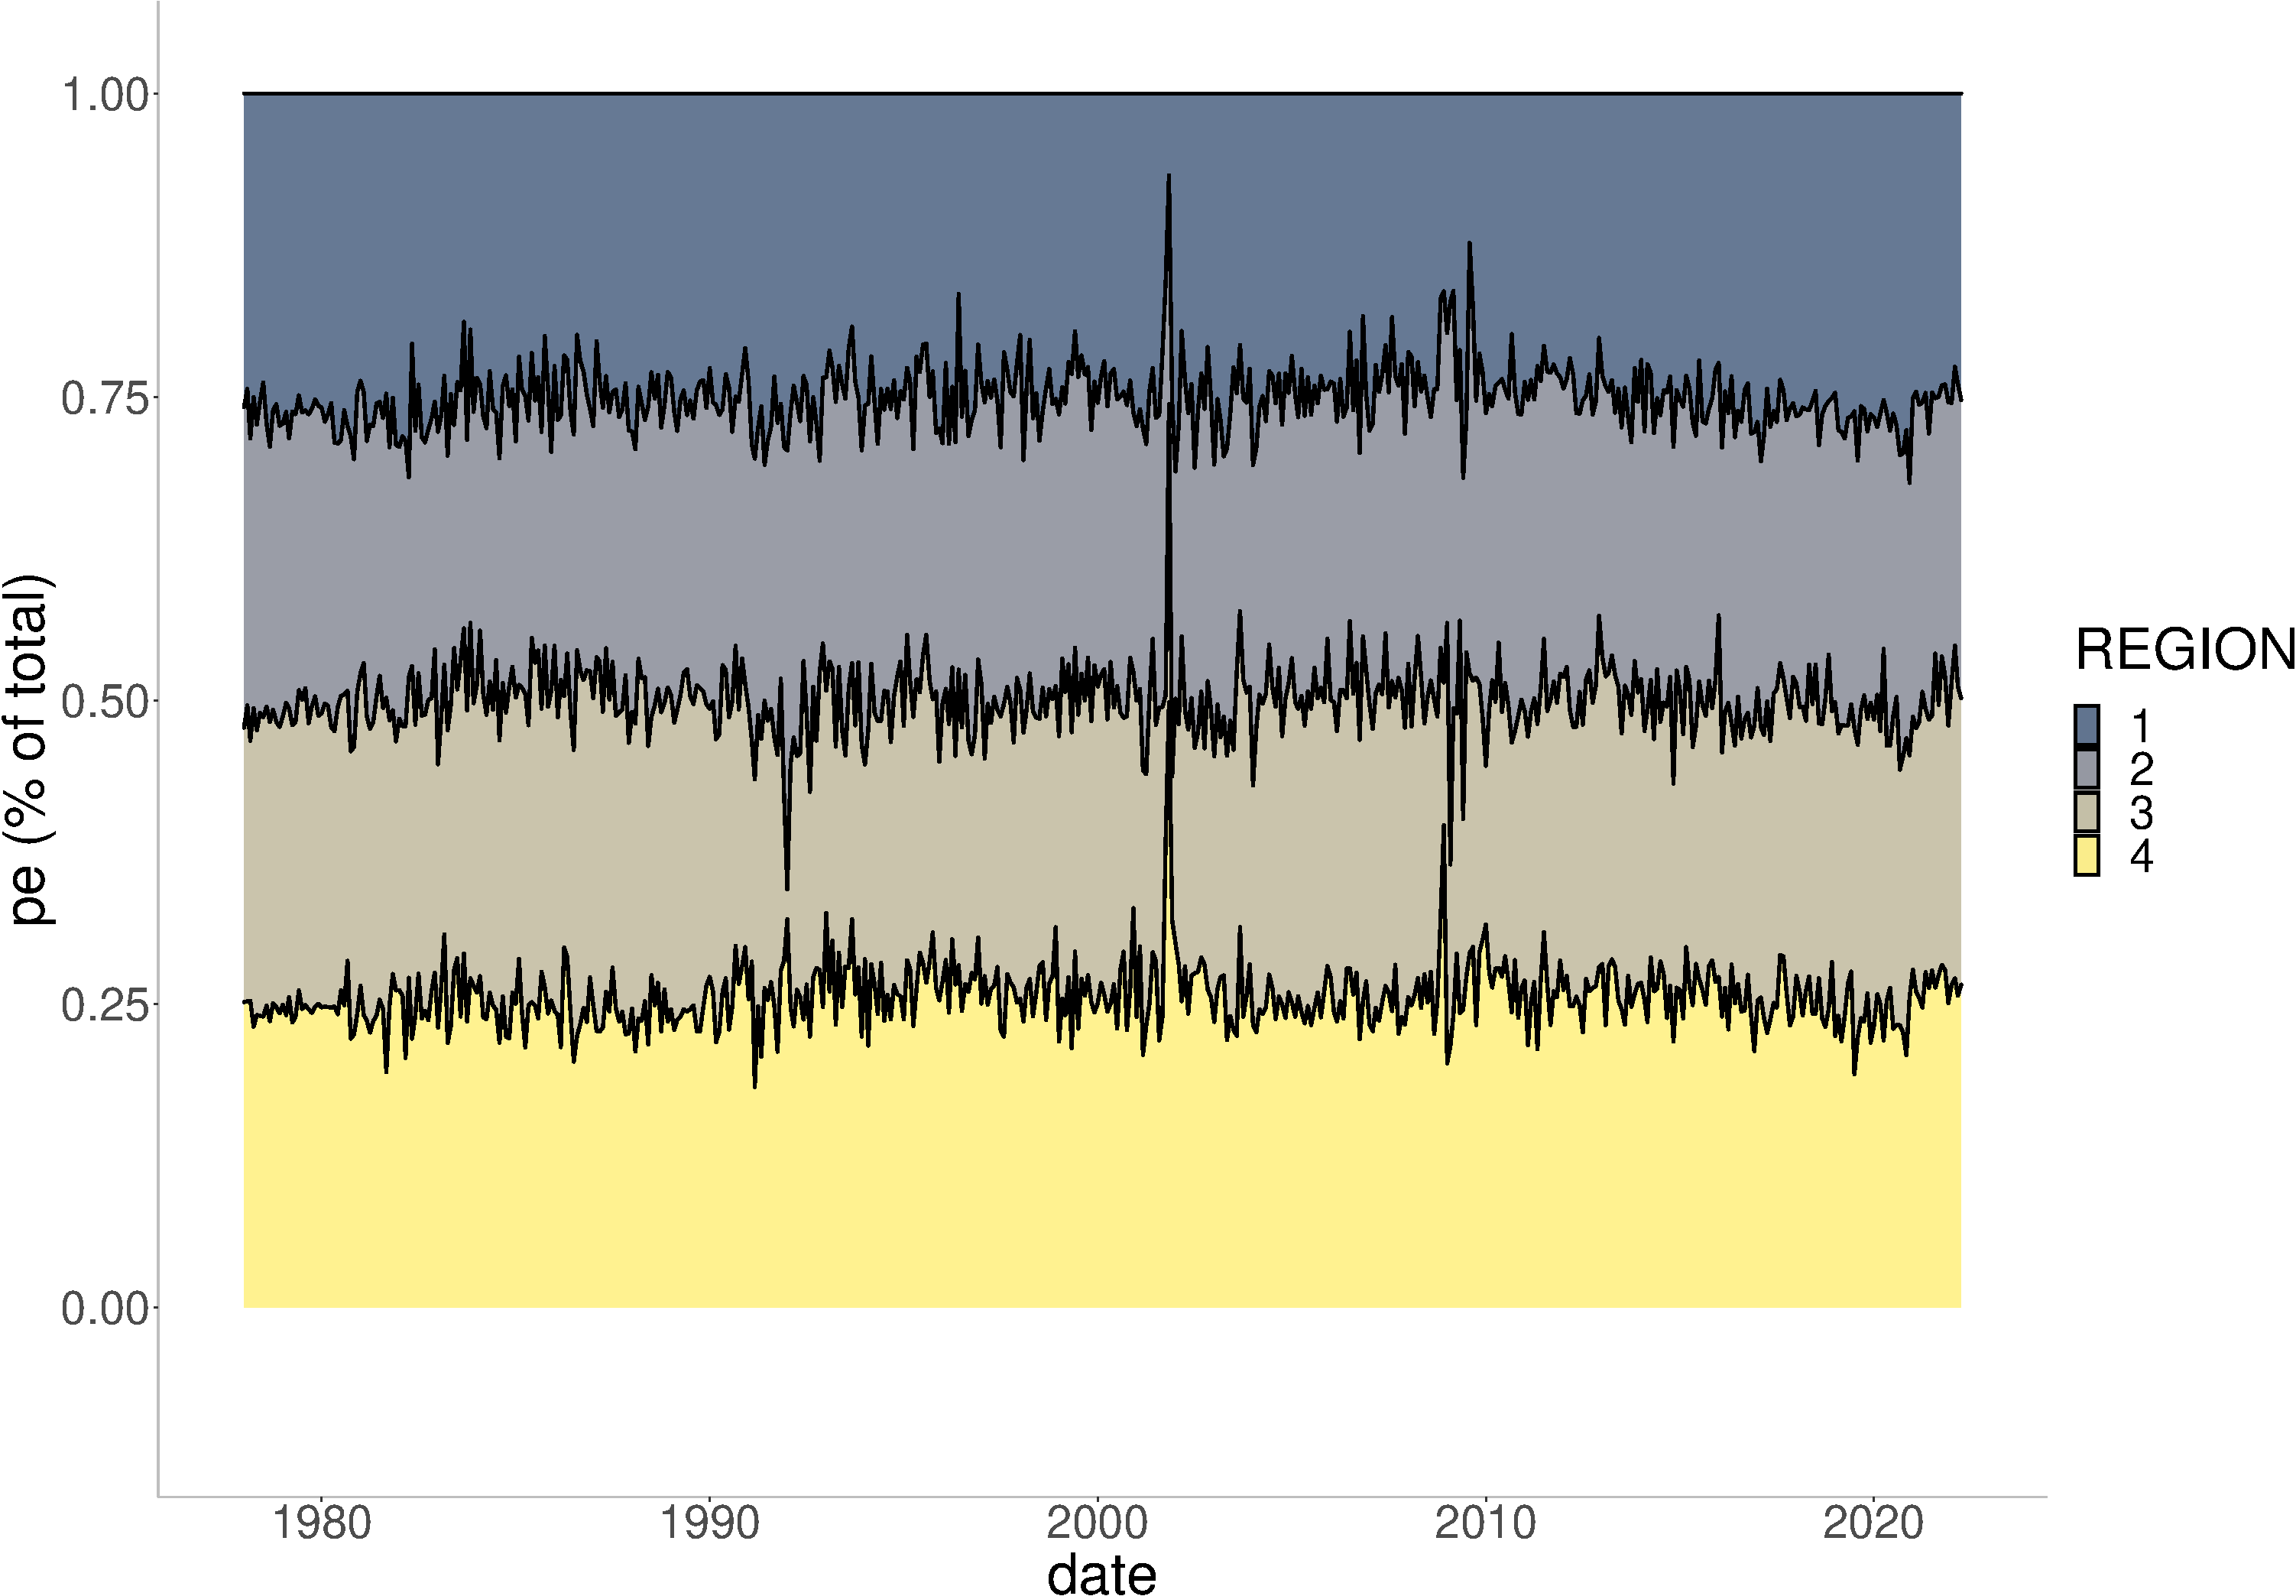
\includegraphics[width =3in, height =2in]{figs/regions}
\caption{Inflation: U.S. regions}\label{fig:intro:RegInf}
\end{subfigure}
\end{figure}

\begin{figure}
\centering
\caption{Diversity of inflation survey expectations: by groups}\label{fig:intro2}
\begin{subfigure}[t]{0.75\textwidth}
%\centering
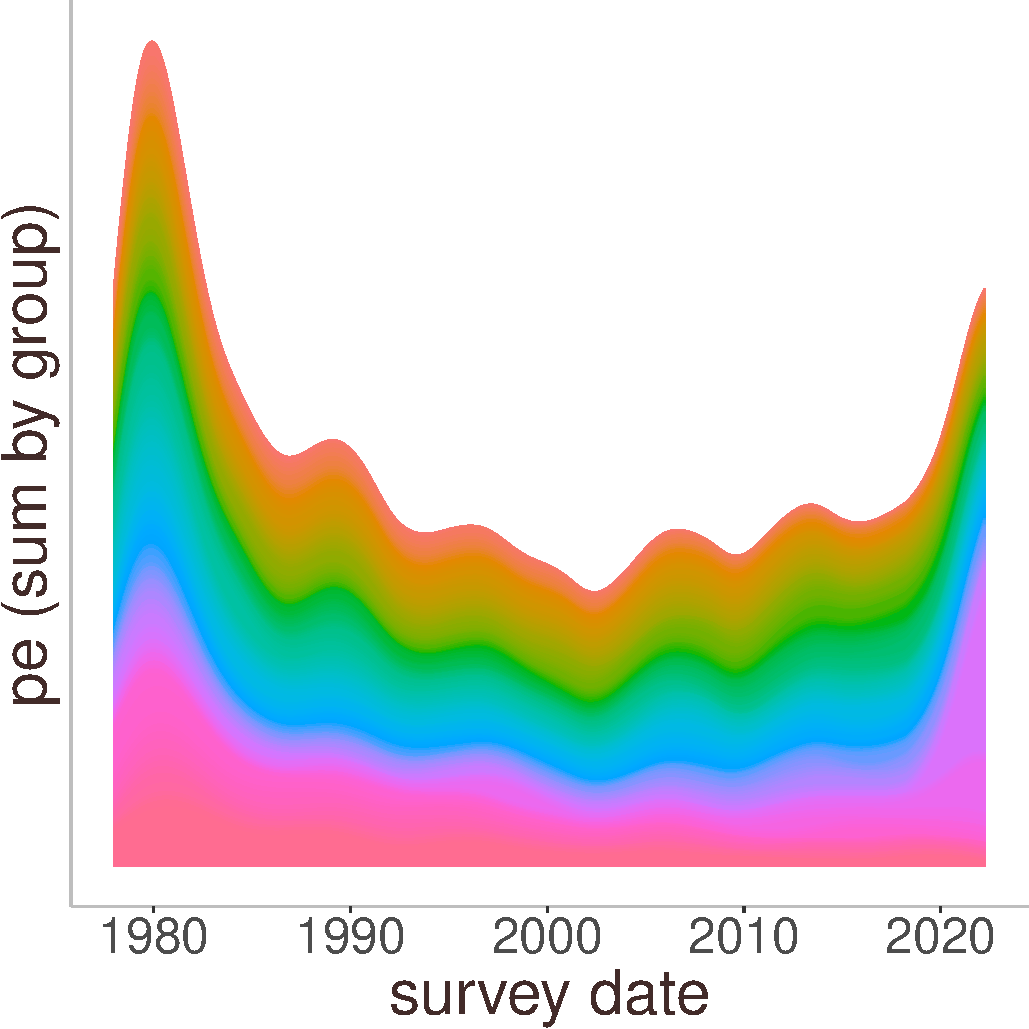
\includegraphics[width = 6.5in, height =3in]{figs/aggIndComp}
\caption{Inflation expectations: all groups. Height = sum of expect.'s.}\label{fig:groupExpects}
\end{subfigure}
\vfill
\begin{subfigure}[t]{0.75\textwidth}
%\centering
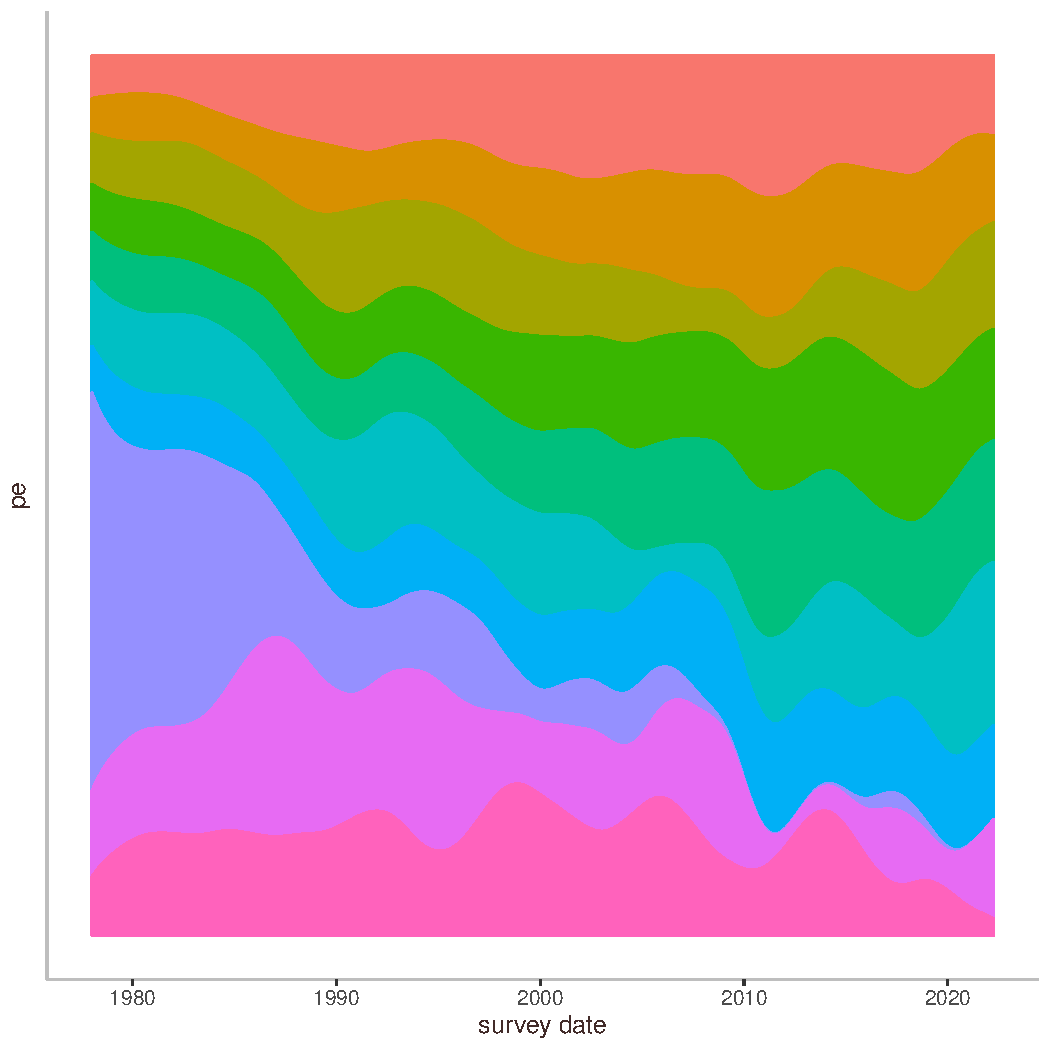
\includegraphics[width = 6.5in, height =3in]{figs/weightsTop10comp}
\caption{Inflation expectations: key groups.}\label{fig:top10Expects}
\end{subfigure}
\end{figure}


Figure \ref{fig:intro2} aids in visualizing the heterogeneity across various groups. Panel \ref{fig:groupExpects} presents a stacked stream plot of the inflation expectations of each of the 160 groups. Finally, panel \ref{fig:top10Expects} focuses on the ten groups that the empirical analysis identifies as particularly important and again plots the proportional share of the (unweighted) average. Aggregate expectations are computed by averaging across regions and groups at each time. The figure plots the sum of these expectations for each survey month. The height of each group's section of the curve represents the average inflation expectation of that group. The relative height, and share of the sum, for groups' expectations, vary over time. So it is not just that married women with a college degree have the highest inflation expectations; at times, they do, and other times they do not. 

\section{Empirical model}

\subsection{Motivating theory}

A standard model of Calvo pricing, extended to include multiple sectors, multiple groups of households, and subjective (possibly, non-rational) expectations, shows inflation to be a weighted average of each group's inflation expectation. A region is a closed economy consisting of a continuum of households and firms.\footnote{As motivation for the empirical model, the closed economy assumption is without a loss of generality, and the insights could extend to a currency union. \cite{NakamuraSteinsson:QJE2022} develop such a model and use regional variation to identify the slope of an aggregate Phillips curve under rational expectations.} The households can be classified into $G$ groups. There are $S$ sectors producing a differentiated consumption good. Each household decides on a lifetime consumption plan and a basket of goods. Household groups differ based on their preferences over bundles of consumption goods. Each group consumption basket is a time-invariant fraction of aggregate consumption. The production of consumption goods follows from a technology aggregating sector-specific intermediate goods produced by a continuum of monopolistically competitive firms with a linear production technology using labor as the only input. Intermediate producers face a Calvo risk that, with probability $1-\lambda_j$, the firm will be unable to adjust its price. The environment is standard with two exceptions: (1.) following \cite{Cravinoetal:JME2020} the extent of price stickiness can differ by sector, and (2.) rational expectations are not assumed.

As in \cite{Cravinoetal:JME2020}, there are multiple price indexes. There is the aggregate price index for consumption goods across sectors, $P_t$, as well as the household group $g\in G$ price index $P_t(g)$ that represents the cost of consuming group $g$'s bundle. Let $\theta$ denote the constant elasticity of substitution between goods. Group $g$'s price index is defined to be
$$ P_t(g) = \left( \sum_s \phi_s(g)P^{1-\theta}_{s,t}\right)^{1/(1-\theta)}$$
where $\phi_s(g)$ is a group-g specific preference parameter for consumption good $s$. The aggregate demand for consumption goods in sector $s$ is
$$ P_{s,t}C_{s,t} = \omega_{s,t}\left(\frac{P_{s,t}}{P_t}\right)^{1-\theta} P_tC_t$$
where $P_t=\left(\sum_s\omega_{s,t}P_{s,t}^{1-\theta}\right)^{1/(1-\theta)}$. The variable $\omega_{s,t}$ is the share of aggregate consumption in sector $s$. It is a weighted average across each household group's preference parameter $\phi_s(g)$, and the weights depend on the group's relative expenditure share. These weights are key to expressing the regional inflation rate in terms of the households' subjective inflation expectations.

Proceeding in the usual way, a firm producing intermediate goods in sector $s$, when allowed to reset prices in time $t$, optimally adjusts its (log) price according to
$$p^*_{s,t} - p_{s,t-1}= \left( 1-\beta\lambda_s\right)\sum_{T=t}^{\infty}\left(\beta\lambda_s\right)^{T-t}\left\{ \left(p^e_{s,T+1}-p_{s,t-1}\right) + w^e_{T}\right\}$$
where $(p^*)^e$ denotes a subjective expectation about own future prices, $w_t$ is the marginal cost (real wage). Price-setting is forward-looking because the Calvo friction gives a probability $1-\lambda_s$ that prices remain fixed in the next period.  

Under rational expectations -- or any theory of expectation formation where subjective beliefs satisfy a law of iterated expectations -- the price-setting rule can be written recursively. However, a specific and simplified assumption on expectation formation is sufficient to motivate the empirical model. As in \cite{Woodford:annualreview}, individuals and firms are ``anticipated utility'' maximizers who may be adjusting (``learning'') their subjective expectations about inflation over time but assume for current decision-making that expected inflation would remain at its present rate. \cite{EvansHonkap-book} refer to this as ``steady-state learning.'' Letting the current inflation expectation, for sector $s$, be denoted as $\pi^e_s$, it follows that expectations about future prices evolve along a linear time trend, i.e. $p^e_{s,t+T} = (1+T)\pi^e_s$.\footnote{A similar simplifying assumption is made by \cite{Werning:expectsWP}.}. The inflation rate in sector $s$ is then
\begin{equation}\label{secPC}
 \pi_{s,t} = \left(1-\beta\lambda_s\right)^{-1} \pi^e_{s} + x_t
 \end{equation}
where $x_t$ is the expected present value of marginal cost factors.

Regional inflation is 
$$\pi^R_t = \sum_{s}\omega_{s,t}\pi_{s,t}$$
and group-specific inflation is
$$ \pi^g_t = \sum_s\omega^g_{s,t}\pi_{s,t}$$
Similarly, suppose that each group's subjective expectation for inflation is an expenditure weighted average of expected inflation rates sector by sector. Let $\Pi^{e'}=\left(\pi^e(g)\right)_{g=1}^{G}, \Pi'_s=\left(\pi^e_s\right)_{s=1}^{S}, \Omega_s' = \left(\left(1-\beta\lambda_s\right)^{-1}\omega^g_s\right)_{s=1}^{S}$, and $\Omega' = \left(\Omega(g)\right)_g$. Then
\begin{equation}\label{Ident}
 \Pi^e = \Omega\Pi_s
\end{equation}
Plugging in for the sector-specific Phillips curves (\ref{secPC}) leads to
\begin{equation}\label{LOM}
\pi^R_t = \Omega_s'\Omega^{-1}\Pi^e_t + x_t
\end{equation}
The regional inflation rate is a weighted average of group-specific inflation rates and other factors that affect prices unrelated to inflation expectations. The weights depend on each sector's shares and the region's group-specific shares.

Similarly, it is possible to differentiate between short and long-run inflation expectations. Suppose that individuals forecast the one period ahead price as $p^e_{s,t+1} = \pi^e_t$ and then longer horizon expectations as before $p^e_{s,t+1+T} = (2+T)\bar{\pi}_s$, with $\bar{\pi}_s$ denoting the long-run inflation expectation for goods in sector $s$. Then
$$ \pi_t^R = \sum_s\omega_{s,t}\left( 1-\beta\lambda_s\right)\pi^e_{s,t+1}+\sum_s\omega_{s,t}\left[1+\left(1-\beta\lambda_s\right)^{-1}\right]\bar{\pi}_s + x_t$$
and so
$$ \pi_t^R = \hat{\Omega}_s'\Omega^{-1}\pi^e_t + \tilde{\Omega}_s'\Omega^{-1}\bar{\pi}+x_t$$
where $\hat{\Omega}'=\left(\omega_s(1-\beta\lambda)\right)_{s}, \tilde{\Omega}' = \left[ \omega_s\left( 1+(1-\beta\lambda )^{-1}\right)\right]$.

In conclusion,
\begin{itemize}
\item The inflation rate, at a regional level, depends positively on subjective inflation expectations.
\item The identifying assumption is given by (\ref{Ident}): group expectations reflect the relative weight of expected inflation in each sector, with the weights capturing heterogeneity in consumption baskets.
\item The strength of the impact of expectations on inflation depends on the extent of price stickiness across sectors, household-group preferences for the consumer goods in various sectors, and the distribution of households across the groups in a region.
\item Household-group expenditure shares depend on the \emph{level} of prices but not the rate of change, i.e., inflation.
\item Although a region is a closed economy, inflation could still depend on aggregate macroeconomic factors, particularly through $x_t$. 
\item Short and long-horizon expectations have different quantitative effects on regional inflation.
\item The empirical strategy exploits variation in sectoral demand within each region to identify the effect inflation expectations have on prices.
\end{itemize}


Firms set prices taking into account expectations of future demand conditions. The left-hand side represents the change in the market clearing price, and the right-hand side represents the expected future prices that a firm might want to set. We use exogenous variation in sectoral demand within each region to identify expected price changes' effect on prices.  

\subsection{Empirical model}

The object of interest is inflation expectations' impact on regional inflation rates. Expectations are endogenous. The identifying assumption is that demographic groups may have distinct preferences for the goods that make up a consumption basket. Their inflation expectations reflect the mix of prices in their basket. Interacting regional group shares with aggregate group inflation expectations instruments for the endogenous expectations. The empirical strategy is a differential exposure design: we identify the impact of expectations by measuring how a region's exposure to aggregate shocks leads to a differentiated inflation response. Each region has differential exposure to the shocks because of different population distributions. The identification strategy is valid so long as the demographic shares satisfy a relevance and an exogeneity condition.

The coefficient of interest is $\beta$ in the equation
\begin{equation}\label{OLS}
 \pi^R_t = \delta_R + \beta \pi^e_{R,t} + \gamma'x_{R,t} + \mu_t + \varepsilon_{R,t}
\end{equation}
where $\pi^R_t$ is the inflation rate in region $R$ at time $t$, $\pi^e_{R,t}$ is the expectation of 12-month ahead regional inflation, $x_{R,t}$ is a vector of controls that includes lags of inflation, $\varepsilon_{R,t}$ is the structural disturbance, $\delta_R, \mu_t$ are region and time fixed effects, respectively. The endogeneity concern is that estimating (\ref{OLS}) via ordinary least squares will produce biased estimates of $\beta$ because $\pi^e_{R,t}$ is endogenous. In particular, endogeneity will arise if expectations respond, after controlling for exogenous covariates $x_{R,t}$, to the factors driving $\varepsilon_{R,t}$.

A shift-share instrument (``Bartik instrument'') addresses the endogeneity. Recall from (\ref{Ident}) that 
$$ \pi^e_{R,t} = \sum_{g}\omega_{R,g,t}\pi^e_{R,g,t}$$
Furthermore, if each region group's inflation expectation decomposes into aggregate and idiosyncratic components, then
$$ \pi^e_{R,g,t} = \pi^e_{g,t} + u_{R,g,t}$$
The empirical strategy uses exogenous variation in $\omega_{R,g,t}$ to generate differential exposure to the group-specific aggregate component $\pi^e_{g,t}$. The instrument is\footnote{The instruments are very closely related to inflation expectations. One concern is that, when calculating $\pi^e_{g,t}$, by averaging over all regions when computing the predicted inflation expectation in a region, the instrument is artificially very highly correlated with the region's inflation expectations. Accordingly, the paper reports results using a ``leave-one-out'' method so that $z_{RT}$ is computed by omitting the region's inflation expectations.}
$$ z_{R,t} = \sum_g \omega_{R,g,t} \pi^e_{g,t}$$

Assuming that $\omega_{R,g,t}$ satisfies strict exogeneity and relevance, then the coefficient $\beta$ can be estimated via 2SLS:
\begin{eqnarray}\label{2SLS}
\pi_{R,t} & = & \beta \pi^e_{R,t} + \gamma'x_{R,t} + \varepsilon_{R,t}\\
\pi^e_{R,t} &=& \zeta z_{R,t} + \phi' x_{R,t} + v_{R,t}
\end{eqnarray}
The vector of exogenous regressors now includes region and time-fixed effects.

The main potential concern which threatens identification is whether group shares predict regional inflation rates through channels other than those posited by the researcher. Here, the channel is different group preferences, and the distribution of groups impacts the level and rate of price changes. That is, the channel is through demand. A reasonable conjecture is that the distribution of groups is endogenous to a region's price level, a cost-of-living measure. However, for identification, it is sufficient that the group shares in a region are exogenous to the change in prices, i.e., inflation (\cite{Pinkhametal:AER2020}). This exogeneity assumption is plausible. However, to make the case convincing, the empirical analysis measures shares using either the beginning of sample population distribution or time-varying survey shares. In the former, those shares are not predictive of the exogenous covariates.

Using the beginning of period shares, and probing the predictive power of those shares, helps allay concerns over whether regional demographics are endogenous to the inflation rate. One plausible story could be that younger and more educated groups tend to live in regions with more dynamic or concentrated industries that experience increasing rates of price changes. In that case, those beginning of period shares would help predict the other variables that also predict inflation.  

In summary, this paper studies the effects of plausibly exogenous shocks to expectations by regression of regional inflation on the predicted inflation expectations using the regional group shares and the aggregate inflation expectations for each group. Essentially, the instrument is a mixed variable that gives the inflation expectations in a region predicted by the aggregate group expectations. The instrument is valid if the group shares in each region are uncorrelated with price supply shocks in the region.

 \subsection{The shift/share instrument}

The empirical strategy exploits that U.S. Census regions have different exposure to the aggregate inflation expectations depicted in Figure \ref{fig:groupExpects}. Again, the identifying assumption is that different groups forecast inflation differently, partly because they consume different baskets of goods. A shift-share instrument can capture this differential exposure by forecasting the regional inflation expectations predicted by a region's (plausibly exogenous) exposure to a group's aggregate inflation expectations shock. The Bartik instrument takes the population share of a particular group in a region and interacts it with that group's aggregate inflation expectations. In particular, the shift variable is the inflation expectations in Figure \ref{fig:groupExpects}. The shares, $\omega_{R,g,t}$, capture the share of the population in region $R$ by group $g$ at time $t$.  

The group share measure is the share of each region's group during month $t$, calculated two ways. The preferred measure, based on convention, is to use time-invariant population shares from the beginning of the sample. The U.S. Census January 1978 Current Population Survey (CPS) provides these measurements by Census region. It seems reasonable to expect that these initial population shares are exogenous to subsequent inflation shocks and price changes. Indeed, empirically these shares have no predictive power for the covariates of inflation over the sample period.  

The second measure uses shares calculated directly from the Michigan survey. Since the Michigan survey aims for a nationally representative sample, the shares should only differ from actual population shares by sampling error, which is plausibly exogenous with unobserved factors driving inflation. That being said, there are two cases to note. First is the re-interviewing of previous respondents and the potential endogeneity of the response rate. The robustness of the coefficient estimates to a specification with first-time respondents only alleviates this concern. Second, it is plausible that an individual may move through groups over time and in response to a region's economy and inflation rate. Since the panel consists of groups rather than individuals, evolving group composition is not a particularly great concern except for those repeating respondents. Again, robustness to first-time respondents can address this potential concern.

\begin{figure}
\centering
\caption{Calculated group shares.}\label{fig:shares}
\begin{subfigure}[t]{\textwidth}
\centering
%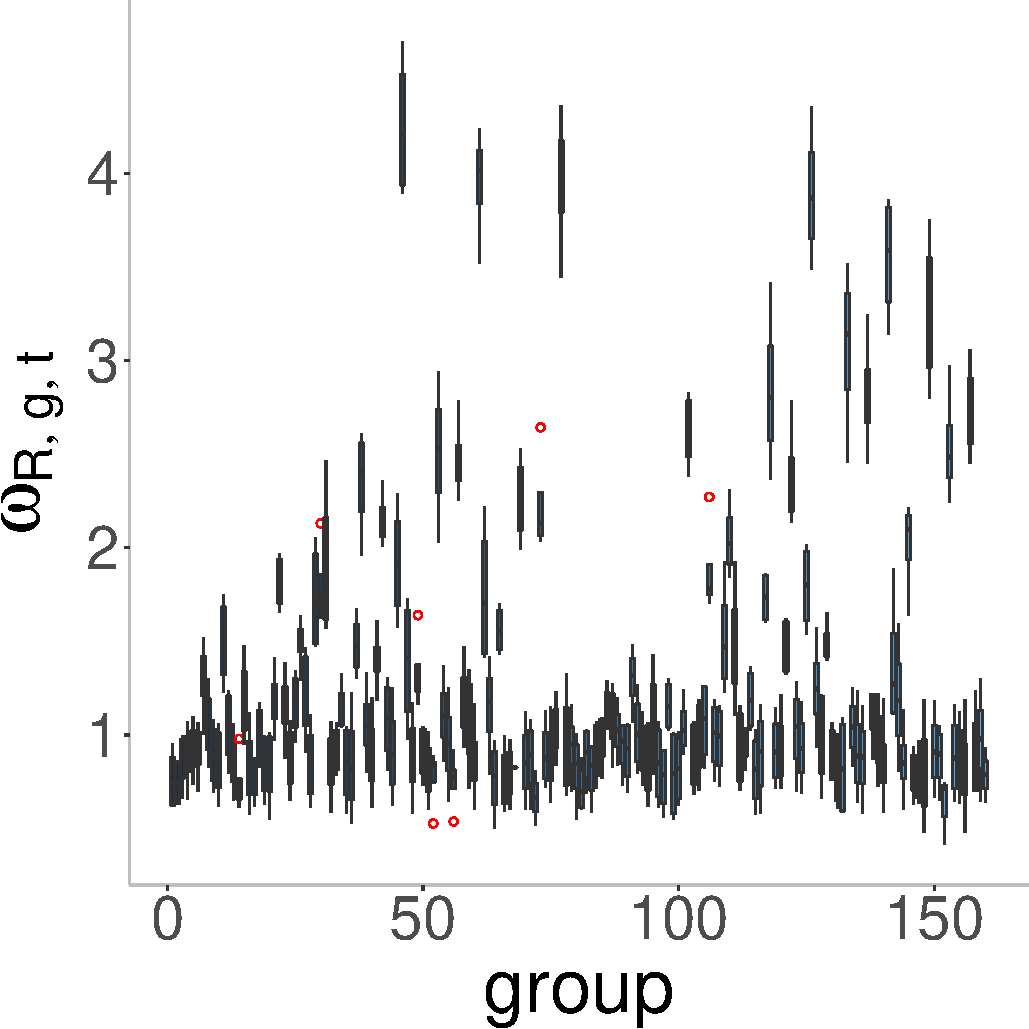
\includegraphics[width = 5in, height =3in]{figs/weightsDiverse}
% Created by tikzDevice version 0.12.3.1 on 2023-11-03 10:48:02
% !TEX encoding = UTF-8 Unicode
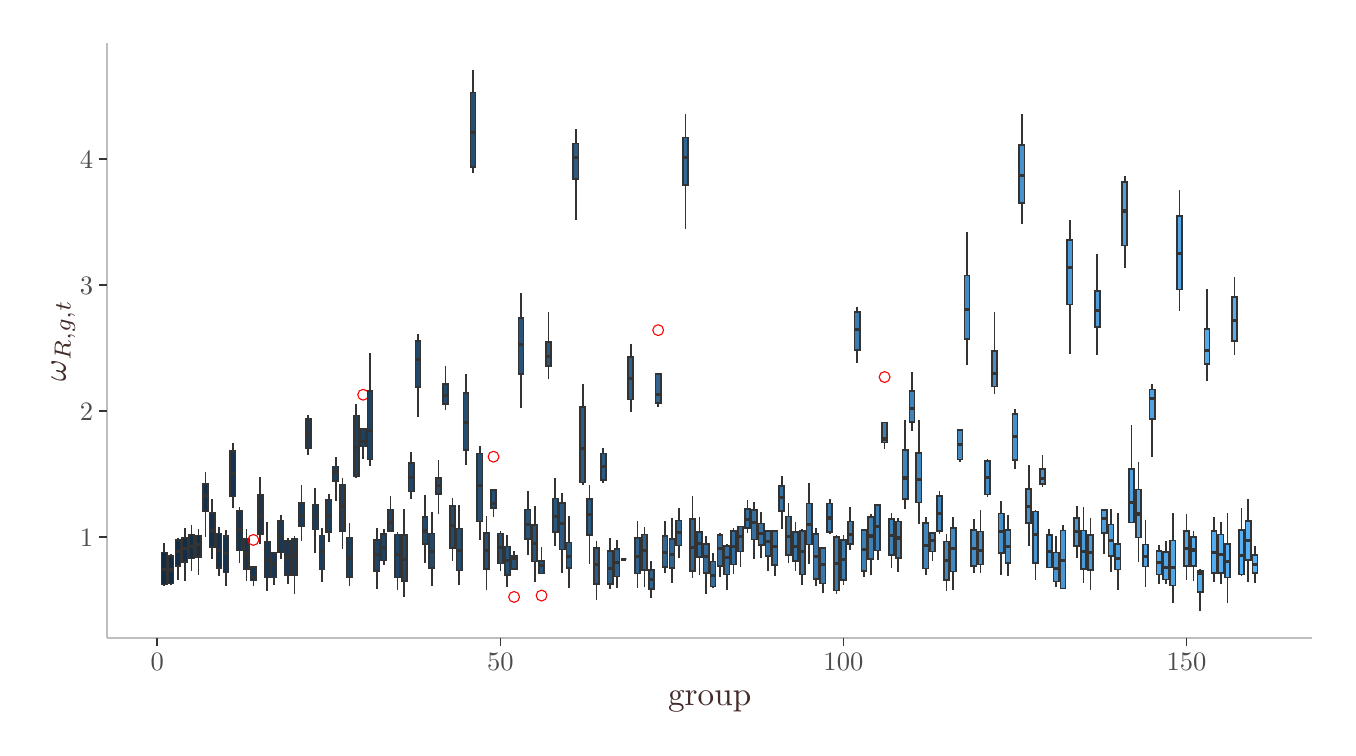
\begin{tikzpicture}[x=1pt,y=1pt]
\definecolor{fillColor}{RGB}{255,255,255}
\path[use as bounding box,fill=fillColor,fill opacity=0.00] (0,0) rectangle (469.75,252.94);
\begin{scope}
\path[clip] (  0.00,  0.00) rectangle (469.75,252.94);
\definecolor{drawColor}{RGB}{255,255,255}
\definecolor{fillColor}{RGB}{255,255,255}

\path[draw=drawColor,line width= 0.6pt,line join=round,line cap=round,fill=fillColor] (  0.00,  0.00) rectangle (469.76,252.94);
\end{scope}
\begin{scope}
\path[clip] ( 28.60, 32.28) rectangle (464.25,247.44);
\definecolor{drawColor}{RGB}{255,255,255}

\path[draw=drawColor,line width= 0.6pt,line join=round] ( 28.60, 68.78) --
	(464.25, 68.78);

\path[draw=drawColor,line width= 0.6pt,line join=round] ( 28.60,114.35) --
	(464.25,114.35);

\path[draw=drawColor,line width= 0.6pt,line join=round] ( 28.60,159.93) --
	(464.25,159.93);

\path[draw=drawColor,line width= 0.6pt,line join=round] ( 28.60,205.51) --
	(464.25,205.51);

\path[draw=drawColor,line width= 0.6pt,line join=round] ( 46.85, 32.28) --
	( 46.85,247.44);

\path[draw=drawColor,line width= 0.6pt,line join=round] (170.81, 32.28) --
	(170.81,247.44);

\path[draw=drawColor,line width= 0.6pt,line join=round] (294.77, 32.28) --
	(294.77,247.44);

\path[draw=drawColor,line width= 0.6pt,line join=round] (418.73, 32.28) --
	(418.73,247.44);
\definecolor{drawColor}{gray}{0.20}

\path[draw=drawColor,line width= 0.6pt,line join=round] ( 49.33, 63.31) -- ( 49.33, 66.76);

\path[draw=drawColor,line width= 0.6pt,line join=round] ( 49.33, 51.72) -- ( 49.33, 51.31);
\definecolor{fillColor}{RGB}{19,43,67}

\path[draw=drawColor,line width= 0.6pt,fill=fillColor] ( 48.40, 63.31) --
	( 48.40, 51.72) --
	( 50.26, 51.72) --
	( 50.26, 63.31) --
	( 48.40, 63.31) --
	cycle;

\path[draw=drawColor,line width= 1.1pt] ( 48.40, 57.01) -- ( 50.26, 57.01);

\path[draw=drawColor,line width= 0.6pt,line join=round] ( 51.81, 62.06) -- ( 51.81, 62.68);

\path[draw=drawColor,line width= 0.6pt,line join=round] ( 51.81, 52.08) -- ( 51.81, 52.07);
\definecolor{fillColor}{RGB}{19,44,68}

\path[draw=drawColor,line width= 0.6pt,fill=fillColor] ( 50.88, 62.06) --
	( 50.88, 52.08) --
	( 52.74, 52.08) --
	( 52.74, 62.06) --
	( 50.88, 62.06) --
	cycle;

\path[draw=drawColor,line width= 1.1pt] ( 50.88, 56.97) -- ( 52.74, 56.97);

\path[draw=drawColor,line width= 0.6pt,line join=round] ( 54.29, 67.76) -- ( 54.29, 68.60);

\path[draw=drawColor,line width= 0.6pt,line join=round] ( 54.29, 58.32) -- ( 54.29, 53.37);
\definecolor{fillColor}{RGB}{20,44,69}

\path[draw=drawColor,line width= 0.6pt,fill=fillColor] ( 53.36, 67.76) --
	( 53.36, 58.32) --
	( 55.22, 58.32) --
	( 55.22, 67.76) --
	( 53.36, 67.76) --
	cycle;

\path[draw=drawColor,line width= 1.1pt] ( 53.36, 63.73) -- ( 55.22, 63.73);

\path[draw=drawColor,line width= 0.6pt,line join=round] ( 56.77, 68.45) -- ( 56.77, 72.10);

\path[draw=drawColor,line width= 0.6pt,line join=round] ( 56.77, 59.86) -- ( 56.77, 53.17);
\definecolor{fillColor}{RGB}{20,45,70}

\path[draw=drawColor,line width= 0.6pt,fill=fillColor] ( 55.84, 68.45) --
	( 55.84, 59.86) --
	( 57.70, 59.86) --
	( 57.70, 68.45) --
	( 55.84, 68.45) --
	cycle;

\path[draw=drawColor,line width= 1.1pt] ( 55.84, 64.66) -- ( 57.70, 64.66);

\path[draw=drawColor,line width= 0.6pt,line join=round] ( 59.25, 69.75) -- ( 59.25, 73.17);

\path[draw=drawColor,line width= 0.6pt,line join=round] ( 59.25, 61.08) -- ( 59.25, 56.76);
\definecolor{fillColor}{RGB}{20,46,71}

\path[draw=drawColor,line width= 0.6pt,fill=fillColor] ( 58.32, 69.75) --
	( 58.32, 61.08) --
	( 60.18, 61.08) --
	( 60.18, 69.75) --
	( 58.32, 69.75) --
	cycle;

\path[draw=drawColor,line width= 1.1pt] ( 58.32, 65.57) -- ( 60.18, 65.57);

\path[draw=drawColor,line width= 0.6pt,line join=round] ( 61.72, 69.42) -- ( 61.72, 71.77);

\path[draw=drawColor,line width= 0.6pt,line join=round] ( 61.72, 61.60) -- ( 61.72, 55.08);
\definecolor{fillColor}{RGB}{21,47,72}

\path[draw=drawColor,line width= 0.6pt,fill=fillColor] ( 60.79, 69.42) --
	( 60.79, 61.60) --
	( 62.65, 61.60) --
	( 62.65, 69.42) --
	( 60.79, 69.42) --
	cycle;

\path[draw=drawColor,line width= 1.1pt] ( 60.79, 66.20) -- ( 62.65, 66.20);

\path[draw=drawColor,line width= 0.6pt,line join=round] ( 64.20, 87.93) -- ( 64.20, 92.50);

\path[draw=drawColor,line width= 0.6pt,line join=round] ( 64.20, 78.33) -- ( 64.20, 68.97);
\definecolor{fillColor}{RGB}{21,47,73}

\path[draw=drawColor,line width= 0.6pt,fill=fillColor] ( 63.27, 87.93) --
	( 63.27, 78.33) --
	( 65.13, 78.33) --
	( 65.13, 87.93) --
	( 63.27, 87.93) --
	cycle;

\path[draw=drawColor,line width= 1.1pt] ( 63.27, 83.93) -- ( 65.13, 83.93);

\path[draw=drawColor,line width= 0.6pt,line join=round] ( 66.68, 77.57) -- ( 66.68, 82.47);

\path[draw=drawColor,line width= 0.6pt,line join=round] ( 66.68, 65.30) -- ( 66.68, 60.79);
\definecolor{fillColor}{RGB}{22,48,74}

\path[draw=drawColor,line width= 0.6pt,fill=fillColor] ( 65.75, 77.57) --
	( 65.75, 65.30) --
	( 67.61, 65.30) --
	( 67.61, 77.57) --
	( 65.75, 77.57) --
	cycle;

\path[draw=drawColor,line width= 1.1pt] ( 65.75, 71.37) -- ( 67.61, 71.37);

\path[draw=drawColor,line width= 0.6pt,line join=round] ( 69.16, 70.17) -- ( 69.16, 72.48);

\path[draw=drawColor,line width= 0.6pt,line join=round] ( 69.16, 57.70) -- ( 69.16, 54.89);
\definecolor{fillColor}{RGB}{22,49,75}

\path[draw=drawColor,line width= 0.6pt,fill=fillColor] ( 68.23, 70.17) --
	( 68.23, 57.70) --
	( 70.09, 57.70) --
	( 70.09, 70.17) --
	( 68.23, 70.17) --
	cycle;

\path[draw=drawColor,line width= 1.1pt] ( 68.23, 64.02) -- ( 70.09, 64.02);

\path[draw=drawColor,line width= 0.6pt,line join=round] ( 71.64, 69.25) -- ( 71.64, 71.46);

\path[draw=drawColor,line width= 0.6pt,line join=round] ( 71.64, 56.09) -- ( 71.64, 51.27);
\definecolor{fillColor}{RGB}{22,50,76}

\path[draw=drawColor,line width= 0.6pt,fill=fillColor] ( 70.71, 69.25) --
	( 70.71, 56.09) --
	( 72.57, 56.09) --
	( 72.57, 69.25) --
	( 70.71, 69.25) --
	cycle;

\path[draw=drawColor,line width= 1.1pt] ( 70.71, 63.10) -- ( 72.57, 63.10);

\path[draw=drawColor,line width= 0.6pt,line join=round] ( 74.12, 99.91) -- ( 74.12,102.91);

\path[draw=drawColor,line width= 0.6pt,line join=round] ( 74.12, 83.55) -- ( 74.12, 79.21);
\definecolor{fillColor}{RGB}{23,50,77}

\path[draw=drawColor,line width= 0.6pt,fill=fillColor] ( 73.19, 99.91) --
	( 73.19, 83.55) --
	( 75.05, 83.55) --
	( 75.05, 99.91) --
	( 73.19, 99.91) --
	cycle;

\path[draw=drawColor,line width= 1.1pt] ( 73.19, 91.96) -- ( 75.05, 91.96);

\path[draw=drawColor,line width= 0.6pt,line join=round] ( 76.60, 78.25) -- ( 76.60, 79.59);

\path[draw=drawColor,line width= 0.6pt,line join=round] ( 76.60, 63.99) -- ( 76.60, 59.42);
\definecolor{fillColor}{RGB}{23,51,78}

\path[draw=drawColor,line width= 0.6pt,fill=fillColor] ( 75.67, 78.25) --
	( 75.67, 63.99) --
	( 77.53, 63.99) --
	( 77.53, 78.25) --
	( 75.67, 78.25) --
	cycle;

\path[draw=drawColor,line width= 1.1pt] ( 75.67, 71.66) -- ( 77.53, 71.66);

\path[draw=drawColor,line width= 0.6pt,line join=round] ( 79.08, 68.41) -- ( 79.08, 71.70);

\path[draw=drawColor,line width= 0.6pt,line join=round] ( 79.08, 57.38) -- ( 79.08, 52.83);
\definecolor{fillColor}{RGB}{24,52,79}

\path[draw=drawColor,line width= 0.6pt,fill=fillColor] ( 78.15, 68.41) --
	( 78.15, 57.38) --
	( 80.01, 57.38) --
	( 80.01, 68.41) --
	( 78.15, 68.41) --
	cycle;

\path[draw=drawColor,line width= 1.1pt] ( 78.15, 63.10) -- ( 80.01, 63.10);
\definecolor{drawColor}{RGB}{255,0,0}

\path[draw=drawColor,line width= 0.4pt,line join=round,line cap=round] ( 81.56, 67.84) circle (  1.96);
\definecolor{drawColor}{gray}{0.20}

\path[draw=drawColor,line width= 0.6pt,line join=round] ( 81.56, 58.14) -- ( 81.56, 58.14);

\path[draw=drawColor,line width= 0.6pt,line join=round] ( 81.56, 53.22) -- ( 81.56, 51.02);
\definecolor{fillColor}{RGB}{24,53,80}

\path[draw=drawColor,line width= 0.6pt,fill=fillColor] ( 80.63, 58.14) --
	( 80.63, 53.22) --
	( 82.49, 53.22) --
	( 82.49, 58.14) --
	( 80.63, 58.14) --
	cycle;

\path[draw=drawColor,line width= 1.1pt] ( 80.63, 54.43) -- ( 82.49, 54.43);

\path[draw=drawColor,line width= 0.6pt,line join=round] ( 84.04, 84.23) -- ( 84.04, 90.49);

\path[draw=drawColor,line width= 0.6pt,line join=round] ( 84.04, 69.95) -- ( 84.04, 66.51);
\definecolor{fillColor}{RGB}{24,53,81}

\path[draw=drawColor,line width= 0.6pt,fill=fillColor] ( 83.11, 84.23) --
	( 83.11, 69.95) --
	( 84.97, 69.95) --
	( 84.97, 84.23) --
	( 83.11, 84.23) --
	cycle;

\path[draw=drawColor,line width= 1.1pt] ( 83.11, 76.62) -- ( 84.97, 76.62);

\path[draw=drawColor,line width= 0.6pt,line join=round] ( 86.52, 67.23) -- ( 86.52, 74.14);

\path[draw=drawColor,line width= 0.6pt,line join=round] ( 86.52, 54.28) -- ( 86.52, 49.52);
\definecolor{fillColor}{RGB}{25,54,82}

\path[draw=drawColor,line width= 0.6pt,fill=fillColor] ( 85.59, 67.23) --
	( 85.59, 54.28) --
	( 87.45, 54.28) --
	( 87.45, 67.23) --
	( 85.59, 67.23) --
	cycle;

\path[draw=drawColor,line width= 1.1pt] ( 85.59, 60.40) -- ( 87.45, 60.40);

\path[draw=drawColor,line width= 0.6pt,line join=round] ( 89.00, 63.12) -- ( 89.00, 63.34);

\path[draw=drawColor,line width= 0.6pt,line join=round] ( 89.00, 54.21) -- ( 89.00, 51.47);
\definecolor{fillColor}{RGB}{25,55,83}

\path[draw=drawColor,line width= 0.6pt,fill=fillColor] ( 88.07, 63.12) --
	( 88.07, 54.21) --
	( 89.93, 54.21) --
	( 89.93, 63.12) --
	( 88.07, 63.12) --
	cycle;

\path[draw=drawColor,line width= 1.1pt] ( 88.07, 59.08) -- ( 89.93, 59.08);

\path[draw=drawColor,line width= 0.6pt,line join=round] ( 91.48, 74.67) -- ( 91.48, 76.76);

\path[draw=drawColor,line width= 0.6pt,line join=round] ( 91.48, 63.45) -- ( 91.48, 60.90);
\definecolor{fillColor}{RGB}{25,56,84}

\path[draw=drawColor,line width= 0.6pt,fill=fillColor] ( 90.55, 74.67) --
	( 90.55, 63.45) --
	( 92.40, 63.45) --
	( 92.40, 74.67) --
	( 90.55, 74.67) --
	cycle;

\path[draw=drawColor,line width= 1.1pt] ( 90.55, 69.14) -- ( 92.40, 69.14);

\path[draw=drawColor,line width= 0.6pt,line join=round] ( 93.95, 67.34) -- ( 93.95, 68.56);

\path[draw=drawColor,line width= 0.6pt,line join=round] ( 93.95, 55.24) -- ( 93.95, 51.81);
\definecolor{fillColor}{RGB}{26,56,85}

\path[draw=drawColor,line width= 0.6pt,fill=fillColor] ( 93.02, 67.34) --
	( 93.02, 55.24) --
	( 94.88, 55.24) --
	( 94.88, 67.34) --
	( 93.02, 67.34) --
	cycle;

\path[draw=drawColor,line width= 1.1pt] ( 93.02, 61.66) -- ( 94.88, 61.66);

\path[draw=drawColor,line width= 0.6pt,line join=round] ( 96.43, 68.29) -- ( 96.43, 69.28);

\path[draw=drawColor,line width= 0.6pt,line join=round] ( 96.43, 55.12) -- ( 96.43, 48.12);
\definecolor{fillColor}{RGB}{26,57,86}

\path[draw=drawColor,line width= 0.6pt,fill=fillColor] ( 95.50, 68.29) --
	( 95.50, 55.12) --
	( 97.36, 55.12) --
	( 97.36, 68.29) --
	( 95.50, 68.29) --
	cycle;

\path[draw=drawColor,line width= 1.1pt] ( 95.50, 62.70) -- ( 97.36, 62.70);

\path[draw=drawColor,line width= 0.6pt,line join=round] ( 98.91, 81.07) -- ( 98.91, 87.72);

\path[draw=drawColor,line width= 0.6pt,line join=round] ( 98.91, 72.74) -- ( 98.91, 67.49);
\definecolor{fillColor}{RGB}{27,58,87}

\path[draw=drawColor,line width= 0.6pt,fill=fillColor] ( 97.98, 81.07) --
	( 97.98, 72.74) --
	( 99.84, 72.74) --
	( 99.84, 81.07) --
	( 97.98, 81.07) --
	cycle;

\path[draw=drawColor,line width= 1.1pt] ( 97.98, 76.67) -- ( 99.84, 76.67);

\path[draw=drawColor,line width= 0.6pt,line join=round] (101.39,111.52) -- (101.39,112.96);

\path[draw=drawColor,line width= 0.6pt,line join=round] (101.39,100.85) -- (101.39, 98.65);
\definecolor{fillColor}{RGB}{27,59,88}

\path[draw=drawColor,line width= 0.6pt,fill=fillColor] (100.46,111.52) --
	(100.46,100.85) --
	(102.32,100.85) --
	(102.32,111.52) --
	(100.46,111.52) --
	cycle;

\path[draw=drawColor,line width= 1.1pt] (100.46,106.31) -- (102.32,106.31);

\path[draw=drawColor,line width= 0.6pt,line join=round] (103.87, 80.50) -- (103.87, 86.54);

\path[draw=drawColor,line width= 0.6pt,line join=round] (103.87, 71.56) -- (103.87, 63.04);
\definecolor{fillColor}{RGB}{27,60,89}

\path[draw=drawColor,line width= 0.6pt,fill=fillColor] (102.94, 80.50) --
	(102.94, 71.56) --
	(104.80, 71.56) --
	(104.80, 80.50) --
	(102.94, 80.50) --
	cycle;

\path[draw=drawColor,line width= 1.1pt] (102.94, 76.45) -- (104.80, 76.45);

\path[draw=drawColor,line width= 0.6pt,line join=round] (106.35, 69.47) -- (106.35, 72.21);

\path[draw=drawColor,line width= 0.6pt,line join=round] (106.35, 57.12) -- (106.35, 52.79);
\definecolor{fillColor}{RGB}{28,60,90}

\path[draw=drawColor,line width= 0.6pt,fill=fillColor] (105.42, 69.47) --
	(105.42, 57.12) --
	(107.28, 57.12) --
	(107.28, 69.47) --
	(105.42, 69.47) --
	cycle;

\path[draw=drawColor,line width= 1.1pt] (105.42, 63.56) -- (107.28, 63.56);

\path[draw=drawColor,line width= 0.6pt,line join=round] (108.83, 82.40) -- (108.83, 84.37);

\path[draw=drawColor,line width= 0.6pt,line join=round] (108.83, 70.68) -- (108.83, 66.94);
\definecolor{fillColor}{RGB}{28,61,91}

\path[draw=drawColor,line width= 0.6pt,fill=fillColor] (107.90, 82.40) --
	(107.90, 70.68) --
	(109.76, 70.68) --
	(109.76, 82.40) --
	(107.90, 82.40) --
	cycle;

\path[draw=drawColor,line width= 1.1pt] (107.90, 76.83) -- (109.76, 76.83);

\path[draw=drawColor,line width= 0.6pt,line join=round] (111.31, 94.39) -- (111.31, 97.97);

\path[draw=drawColor,line width= 0.6pt,line join=round] (111.31, 89.17) -- (111.31, 81.94);
\definecolor{fillColor}{RGB}{29,62,92}

\path[draw=drawColor,line width= 0.6pt,fill=fillColor] (110.38, 94.39) --
	(110.38, 89.17) --
	(112.24, 89.17) --
	(112.24, 94.39) --
	(110.38, 94.39) --
	cycle;

\path[draw=drawColor,line width= 1.1pt] (110.38, 92.38) -- (112.24, 92.38);

\path[draw=drawColor,line width= 0.6pt,line join=round] (113.79, 87.73) -- (113.79, 90.14);

\path[draw=drawColor,line width= 0.6pt,line join=round] (113.79, 71.04) -- (113.79, 64.53);
\definecolor{fillColor}{RGB}{29,63,93}

\path[draw=drawColor,line width= 0.6pt,fill=fillColor] (112.86, 87.73) --
	(112.86, 71.04) --
	(114.72, 71.04) --
	(114.72, 87.73) --
	(112.86, 87.73) --
	cycle;

\path[draw=drawColor,line width= 1.1pt] (112.86, 80.07) -- (114.72, 80.07);

\path[draw=drawColor,line width= 0.6pt,line join=round] (116.27, 68.74) -- (116.27, 73.86);

\path[draw=drawColor,line width= 0.6pt,line join=round] (116.27, 54.46) -- (116.27, 51.09);
\definecolor{fillColor}{RGB}{29,63,94}

\path[draw=drawColor,line width= 0.6pt,fill=fillColor] (115.34, 68.74) --
	(115.34, 54.46) --
	(117.20, 54.46) --
	(117.20, 68.74) --
	(115.34, 68.74) --
	cycle;

\path[draw=drawColor,line width= 1.1pt] (115.34, 61.31) -- (117.20, 61.31);

\path[draw=drawColor,line width= 0.6pt,line join=round] (118.75,112.81) -- (118.75,116.93);

\path[draw=drawColor,line width= 0.6pt,line join=round] (118.75, 91.03) -- (118.75, 90.27);
\definecolor{fillColor}{RGB}{30,64,96}

\path[draw=drawColor,line width= 0.6pt,fill=fillColor] (117.82,112.81) --
	(117.82, 91.03) --
	(119.68, 91.03) --
	(119.68,112.81) --
	(117.82,112.81) --
	cycle;

\path[draw=drawColor,line width= 1.1pt] (117.82,101.36) -- (119.68,101.36);
\definecolor{drawColor}{RGB}{255,0,0}

\path[draw=drawColor,line width= 0.4pt,line join=round,line cap=round] (121.23,120.30) circle (  1.96);
\definecolor{drawColor}{gray}{0.20}

\path[draw=drawColor,line width= 0.6pt,line join=round] (121.23,107.84) -- (121.23,107.84);

\path[draw=drawColor,line width= 0.6pt,line join=round] (121.23,101.64) -- (121.23, 97.15);
\definecolor{fillColor}{RGB}{30,65,97}

\path[draw=drawColor,line width= 0.6pt,fill=fillColor] (120.30,107.84) --
	(120.30,101.64) --
	(122.16,101.64) --
	(122.16,107.84) --
	(120.30,107.84) --
	cycle;

\path[draw=drawColor,line width= 1.1pt] (120.30,103.41) -- (122.16,103.41);

\path[draw=drawColor,line width= 0.6pt,line join=round] (123.70,121.72) -- (123.70,135.52);

\path[draw=drawColor,line width= 0.6pt,line join=round] (123.70, 96.90) -- (123.70, 94.72);
\definecolor{fillColor}{RGB}{31,66,98}

\path[draw=drawColor,line width= 0.6pt,fill=fillColor] (122.78,121.72) --
	(122.78, 96.90) --
	(124.63, 96.90) --
	(124.63,121.72) --
	(122.78,121.72) --
	cycle;

\path[draw=drawColor,line width= 1.1pt] (122.78,107.38) -- (124.63,107.38);

\path[draw=drawColor,line width= 0.6pt,line join=round] (126.18, 67.84) -- (126.18, 72.13);

\path[draw=drawColor,line width= 0.6pt,line join=round] (126.18, 56.69) -- (126.18, 49.96);
\definecolor{fillColor}{RGB}{31,67,99}

\path[draw=drawColor,line width= 0.6pt,fill=fillColor] (125.25, 67.84) --
	(125.25, 56.69) --
	(127.11, 56.69) --
	(127.11, 67.84) --
	(125.25, 67.84) --
	cycle;

\path[draw=drawColor,line width= 1.1pt] (125.25, 62.67) -- (127.11, 62.67);

\path[draw=drawColor,line width= 0.6pt,line join=round] (128.66, 69.89) -- (128.66, 71.85);

\path[draw=drawColor,line width= 0.6pt,line join=round] (128.66, 60.37) -- (128.66, 58.88);
\definecolor{fillColor}{RGB}{31,67,100}

\path[draw=drawColor,line width= 0.6pt,fill=fillColor] (127.73, 69.89) --
	(127.73, 60.37) --
	(129.59, 60.37) --
	(129.59, 69.89) --
	(127.73, 69.89) --
	cycle;

\path[draw=drawColor,line width= 1.1pt] (127.73, 65.05) -- (129.59, 65.05);

\path[draw=drawColor,line width= 0.6pt,line join=round] (131.14, 78.89) -- (131.14, 83.85);

\path[draw=drawColor,line width= 0.6pt,line join=round] (131.14, 71.17) -- (131.14, 70.71);
\definecolor{fillColor}{RGB}{32,68,101}

\path[draw=drawColor,line width= 0.6pt,fill=fillColor] (130.21, 78.89) --
	(130.21, 71.17) --
	(132.07, 71.17) --
	(132.07, 78.89) --
	(130.21, 78.89) --
	cycle;

\path[draw=drawColor,line width= 1.1pt] (130.21, 74.28) -- (132.07, 74.28);

\path[draw=drawColor,line width= 0.6pt,line join=round] (133.62, 69.82) -- (133.62, 70.82);

\path[draw=drawColor,line width= 0.6pt,line join=round] (133.62, 54.31) -- (133.62, 49.73);
\definecolor{fillColor}{RGB}{32,69,102}

\path[draw=drawColor,line width= 0.6pt,fill=fillColor] (132.69, 69.82) --
	(132.69, 54.31) --
	(134.55, 54.31) --
	(134.55, 69.82) --
	(132.69, 69.82) --
	cycle;

\path[draw=drawColor,line width= 1.1pt] (132.69, 62.66) -- (134.55, 62.66);

\path[draw=drawColor,line width= 0.6pt,line join=round] (136.10, 69.67) -- (136.10, 79.06);

\path[draw=drawColor,line width= 0.6pt,line join=round] (136.10, 53.01) -- (136.10, 47.33);
\definecolor{fillColor}{RGB}{33,70,103}

\path[draw=drawColor,line width= 0.6pt,fill=fillColor] (135.17, 69.67) --
	(135.17, 53.01) --
	(137.03, 53.01) --
	(137.03, 69.67) --
	(135.17, 69.67) --
	cycle;

\path[draw=drawColor,line width= 1.1pt] (135.17, 60.72) -- (137.03, 60.72);

\path[draw=drawColor,line width= 0.6pt,line join=round] (138.58, 95.72) -- (138.58, 99.48);

\path[draw=drawColor,line width= 0.6pt,line join=round] (138.58, 85.32) -- (138.58, 82.53);
\definecolor{fillColor}{RGB}{33,70,104}

\path[draw=drawColor,line width= 0.6pt,fill=fillColor] (137.65, 95.72) --
	(137.65, 85.32) --
	(139.51, 85.32) --
	(139.51, 95.72) --
	(137.65, 95.72) --
	cycle;

\path[draw=drawColor,line width= 1.1pt] (137.65, 90.35) -- (139.51, 90.35);

\path[draw=drawColor,line width= 0.6pt,line join=round] (141.06,139.82) -- (141.06,142.20);

\path[draw=drawColor,line width= 0.6pt,line join=round] (141.06,123.21) -- (141.06,112.39);
\definecolor{fillColor}{RGB}{33,71,105}

\path[draw=drawColor,line width= 0.6pt,fill=fillColor] (140.13,139.82) --
	(140.13,123.21) --
	(141.99,123.21) --
	(141.99,139.82) --
	(140.13,139.82) --
	cycle;

\path[draw=drawColor,line width= 1.1pt] (140.13,132.92) -- (141.99,132.92);

\path[draw=drawColor,line width= 0.6pt,line join=round] (143.54, 76.21) -- (143.54, 83.91);

\path[draw=drawColor,line width= 0.6pt,line join=round] (143.54, 66.27) -- (143.54, 59.65);
\definecolor{fillColor}{RGB}{34,72,106}

\path[draw=drawColor,line width= 0.6pt,fill=fillColor] (142.61, 76.21) --
	(142.61, 66.27) --
	(144.47, 66.27) --
	(144.47, 76.21) --
	(142.61, 76.21) --
	cycle;

\path[draw=drawColor,line width= 1.1pt] (142.61, 71.06) -- (144.47, 71.06);

\path[draw=drawColor,line width= 0.6pt,line join=round] (146.02, 70.12) -- (146.02, 77.95);

\path[draw=drawColor,line width= 0.6pt,line join=round] (146.02, 57.68) -- (146.02, 51.08);
\definecolor{fillColor}{RGB}{34,73,107}

\path[draw=drawColor,line width= 0.6pt,fill=fillColor] (145.09, 70.12) --
	(145.09, 57.68) --
	(146.95, 57.68) --
	(146.95, 70.12) --
	(145.09, 70.12) --
	cycle;

\path[draw=drawColor,line width= 1.1pt] (145.09, 63.69) -- (146.95, 63.69);

\path[draw=drawColor,line width= 0.6pt,line join=round] (148.50, 90.15) -- (148.50, 96.71);

\path[draw=drawColor,line width= 0.6pt,line join=round] (148.50, 84.37) -- (148.50, 77.22);
\definecolor{fillColor}{RGB}{34,74,108}

\path[draw=drawColor,line width= 0.6pt,fill=fillColor] (147.57, 90.15) --
	(147.57, 84.37) --
	(149.43, 84.37) --
	(149.43, 90.15) --
	(147.57, 90.15) --
	cycle;

\path[draw=drawColor,line width= 1.1pt] (147.57, 87.36) -- (149.43, 87.36);

\path[draw=drawColor,line width= 0.6pt,line join=round] (150.98,124.22) -- (150.98,130.75);

\path[draw=drawColor,line width= 0.6pt,line join=round] (150.98,117.03) -- (150.98,114.73);
\definecolor{fillColor}{RGB}{35,74,109}

\path[draw=drawColor,line width= 0.6pt,fill=fillColor] (150.05,124.22) --
	(150.05,117.03) --
	(151.91,117.03) --
	(151.91,124.22) --
	(150.05,124.22) --
	cycle;

\path[draw=drawColor,line width= 1.1pt] (150.05,119.92) -- (151.91,119.92);

\path[draw=drawColor,line width= 0.6pt,line join=round] (153.46, 80.21) -- (153.46, 82.87);

\path[draw=drawColor,line width= 0.6pt,line join=round] (153.46, 65.00) -- (153.46, 60.20);
\definecolor{fillColor}{RGB}{35,75,110}

\path[draw=drawColor,line width= 0.6pt,fill=fillColor] (152.53, 80.21) --
	(152.53, 65.00) --
	(154.39, 65.00) --
	(154.39, 80.21) --
	(152.53, 80.21) --
	cycle;

\path[draw=drawColor,line width= 1.1pt] (152.53, 72.97) -- (154.39, 72.97);

\path[draw=drawColor,line width= 0.6pt,line join=round] (155.93, 72.00) -- (155.93, 80.31);

\path[draw=drawColor,line width= 0.6pt,line join=round] (155.93, 56.82) -- (155.93, 51.60);
\definecolor{fillColor}{RGB}{36,76,111}

\path[draw=drawColor,line width= 0.6pt,fill=fillColor] (155.00, 72.00) --
	(155.00, 56.82) --
	(156.86, 56.82) --
	(156.86, 72.00) --
	(155.00, 72.00) --
	cycle;

\path[draw=drawColor,line width= 1.1pt] (155.00, 63.90) -- (156.86, 63.90);

\path[draw=drawColor,line width= 0.6pt,line join=round] (158.41,120.81) -- (158.41,127.67);

\path[draw=drawColor,line width= 0.6pt,line join=round] (158.41,100.36) -- (158.41, 94.86);
\definecolor{fillColor}{RGB}{36,77,113}

\path[draw=drawColor,line width= 0.6pt,fill=fillColor] (157.48,120.81) --
	(157.48,100.36) --
	(159.34,100.36) --
	(159.34,120.81) --
	(157.48,120.81) --
	cycle;

\path[draw=drawColor,line width= 1.1pt] (157.48,110.36) -- (159.34,110.36);

\path[draw=drawColor,line width= 0.6pt,line join=round] (160.89,229.48) -- (160.89,237.66);

\path[draw=drawColor,line width= 0.6pt,line join=round] (160.89,202.65) -- (160.89,200.60);
\definecolor{fillColor}{RGB}{37,78,114}

\path[draw=drawColor,line width= 0.6pt,fill=fillColor] (159.96,229.48) --
	(159.96,202.65) --
	(161.82,202.65) --
	(161.82,229.48) --
	(159.96,229.48) --
	cycle;

\path[draw=drawColor,line width= 1.1pt] (159.96,215.04) -- (161.82,215.04);

\path[draw=drawColor,line width= 0.6pt,line join=round] (163.37, 99.03) -- (163.37,101.91);

\path[draw=drawColor,line width= 0.6pt,line join=round] (163.37, 74.54) -- (163.37, 67.66);
\definecolor{fillColor}{RGB}{37,78,115}

\path[draw=drawColor,line width= 0.6pt,fill=fillColor] (162.44, 99.03) --
	(162.44, 74.54) --
	(164.30, 74.54) --
	(164.30, 99.03) --
	(162.44, 99.03) --
	cycle;

\path[draw=drawColor,line width= 1.1pt] (162.44, 87.46) -- (164.30, 87.46);

\path[draw=drawColor,line width= 0.6pt,line join=round] (165.85, 70.29) -- (165.85, 76.62);

\path[draw=drawColor,line width= 0.6pt,line join=round] (165.85, 57.39) -- (165.85, 49.69);
\definecolor{fillColor}{RGB}{37,79,116}

\path[draw=drawColor,line width= 0.6pt,fill=fillColor] (164.92, 70.29) --
	(164.92, 57.39) --
	(166.78, 57.39) --
	(166.78, 70.29) --
	(164.92, 70.29) --
	cycle;

\path[draw=drawColor,line width= 1.1pt] (164.92, 64.07) -- (166.78, 64.07);
\definecolor{drawColor}{RGB}{255,0,0}

\path[draw=drawColor,line width= 0.4pt,line join=round,line cap=round] (168.33, 97.91) circle (  1.96);
\definecolor{drawColor}{gray}{0.20}

\path[draw=drawColor,line width= 0.6pt,line join=round] (168.33, 85.82) -- (168.33, 85.82);

\path[draw=drawColor,line width= 0.6pt,line join=round] (168.33, 79.46) -- (168.33, 76.20);
\definecolor{fillColor}{RGB}{38,80,117}

\path[draw=drawColor,line width= 0.6pt,fill=fillColor] (167.40, 85.82) --
	(167.40, 79.46) --
	(169.26, 79.46) --
	(169.26, 85.82) --
	(167.40, 85.82) --
	cycle;

\path[draw=drawColor,line width= 1.1pt] (167.40, 81.17) -- (169.26, 81.17);

\path[draw=drawColor,line width= 0.6pt,line join=round] (170.81, 70.20) -- (170.81, 70.90);

\path[draw=drawColor,line width= 0.6pt,line join=round] (170.81, 59.35) -- (170.81, 56.60);
\definecolor{fillColor}{RGB}{38,81,118}

\path[draw=drawColor,line width= 0.6pt,fill=fillColor] (169.88, 70.20) --
	(169.88, 59.35) --
	(171.74, 59.35) --
	(171.74, 70.20) --
	(169.88, 70.20) --
	cycle;

\path[draw=drawColor,line width= 1.1pt] (169.88, 65.11) -- (171.74, 65.11);

\path[draw=drawColor,line width= 0.6pt,line join=round] (173.29, 65.52) -- (173.29, 69.58);

\path[draw=drawColor,line width= 0.6pt,line join=round] (173.29, 55.10) -- (173.29, 50.65);
\definecolor{fillColor}{RGB}{39,82,119}

\path[draw=drawColor,line width= 0.6pt,fill=fillColor] (172.36, 65.52) --
	(172.36, 55.10) --
	(174.22, 55.10) --
	(174.22, 65.52) --
	(172.36, 65.52) --
	cycle;

\path[draw=drawColor,line width= 1.1pt] (172.36, 60.37) -- (174.22, 60.37);
\definecolor{drawColor}{RGB}{255,0,0}

\path[draw=drawColor,line width= 0.4pt,line join=round,line cap=round] (175.77, 47.24) circle (  1.96);
\definecolor{drawColor}{gray}{0.20}

\path[draw=drawColor,line width= 0.6pt,line join=round] (175.77, 62.10) -- (175.77, 63.88);

\path[draw=drawColor,line width= 0.6pt,line join=round] (175.77, 57.33) -- (175.77, 57.33);
\definecolor{fillColor}{RGB}{39,82,120}

\path[draw=drawColor,line width= 0.6pt,fill=fillColor] (174.84, 62.10) --
	(174.84, 57.33) --
	(176.70, 57.33) --
	(176.70, 62.10) --
	(174.84, 62.10) --
	cycle;

\path[draw=drawColor,line width= 1.1pt] (174.84, 61.10) -- (176.70, 61.10);

\path[draw=drawColor,line width= 0.6pt,line join=round] (178.25,148.01) -- (178.25,157.13);

\path[draw=drawColor,line width= 0.6pt,line join=round] (178.25,127.72) -- (178.25,115.64);
\definecolor{fillColor}{RGB}{39,83,121}

\path[draw=drawColor,line width= 0.6pt,fill=fillColor] (177.32,148.01) --
	(177.32,127.72) --
	(179.18,127.72) --
	(179.18,148.01) --
	(177.32,148.01) --
	cycle;

\path[draw=drawColor,line width= 1.1pt] (177.32,138.36) -- (179.18,138.36);

\path[draw=drawColor,line width= 0.6pt,line join=round] (180.73, 78.85) -- (180.73, 85.69);

\path[draw=drawColor,line width= 0.6pt,line join=round] (180.73, 68.28) -- (180.73, 62.44);
\definecolor{fillColor}{RGB}{40,84,122}

\path[draw=drawColor,line width= 0.6pt,fill=fillColor] (179.80, 78.85) --
	(179.80, 68.28) --
	(181.66, 68.28) --
	(181.66, 78.85) --
	(179.80, 78.85) --
	cycle;

\path[draw=drawColor,line width= 1.1pt] (179.80, 73.40) -- (181.66, 73.40);

\path[draw=drawColor,line width= 0.6pt,line join=round] (183.21, 73.13) -- (183.21, 80.25);

\path[draw=drawColor,line width= 0.6pt,line join=round] (183.21, 60.08) -- (183.21, 52.71);
\definecolor{fillColor}{RGB}{40,85,123}

\path[draw=drawColor,line width= 0.6pt,fill=fillColor] (182.28, 73.13) --
	(182.28, 60.08) --
	(184.14, 60.08) --
	(184.14, 73.13) --
	(182.28, 73.13) --
	cycle;

\path[draw=drawColor,line width= 1.1pt] (182.28, 66.65) -- (184.14, 66.65);
\definecolor{drawColor}{RGB}{255,0,0}

\path[draw=drawColor,line width= 0.4pt,line join=round,line cap=round] (185.69, 47.73) circle (  1.96);
\definecolor{drawColor}{gray}{0.20}

\path[draw=drawColor,line width= 0.6pt,line join=round] (185.69, 60.25) -- (185.69, 65.18);

\path[draw=drawColor,line width= 0.6pt,line join=round] (185.69, 55.75) -- (185.69, 55.75);
\definecolor{fillColor}{RGB}{41,86,125}

\path[draw=drawColor,line width= 0.6pt,fill=fillColor] (184.76, 60.25) --
	(184.76, 55.75) --
	(186.61, 55.75) --
	(186.61, 60.25) --
	(184.76, 60.25) --
	cycle;

\path[draw=drawColor,line width= 1.1pt] (184.76, 58.51) -- (186.61, 58.51);

\path[draw=drawColor,line width= 0.6pt,line join=round] (188.16,139.30) -- (188.16,150.08);

\path[draw=drawColor,line width= 0.6pt,line join=round] (188.16,130.66) -- (188.16,125.86);
\definecolor{fillColor}{RGB}{41,87,126}

\path[draw=drawColor,line width= 0.6pt,fill=fillColor] (187.23,139.30) --
	(187.23,130.66) --
	(189.09,130.66) --
	(189.09,139.30) --
	(187.23,139.30) --
	cycle;

\path[draw=drawColor,line width= 1.1pt] (187.23,133.99) -- (189.09,133.99);

\path[draw=drawColor,line width= 0.6pt,line join=round] (190.64, 82.79) -- (190.64, 90.26);

\path[draw=drawColor,line width= 0.6pt,line join=round] (190.64, 70.61) -- (190.64, 65.78);
\definecolor{fillColor}{RGB}{41,87,127}

\path[draw=drawColor,line width= 0.6pt,fill=fillColor] (189.71, 82.79) --
	(189.71, 70.61) --
	(191.57, 70.61) --
	(191.57, 82.79) --
	(189.71, 82.79) --
	cycle;

\path[draw=drawColor,line width= 1.1pt] (189.71, 76.26) -- (191.57, 76.26);

\path[draw=drawColor,line width= 0.6pt,line join=round] (193.12, 81.14) -- (193.12, 84.66);

\path[draw=drawColor,line width= 0.6pt,line join=round] (193.12, 64.35) -- (193.12, 55.73);
\definecolor{fillColor}{RGB}{42,88,128}

\path[draw=drawColor,line width= 0.6pt,fill=fillColor] (192.19, 81.14) --
	(192.19, 64.35) --
	(194.05, 64.35) --
	(194.05, 81.14) --
	(192.19, 81.14) --
	cycle;

\path[draw=drawColor,line width= 1.1pt] (192.19, 73.60) -- (194.05, 73.60);

\path[draw=drawColor,line width= 0.6pt,line join=round] (195.60, 66.96) -- (195.60, 76.34);

\path[draw=drawColor,line width= 0.6pt,line join=round] (195.60, 57.72) -- (195.60, 50.55);
\definecolor{fillColor}{RGB}{42,89,129}

\path[draw=drawColor,line width= 0.6pt,fill=fillColor] (194.67, 66.96) --
	(194.67, 57.72) --
	(196.53, 57.72) --
	(196.53, 66.96) --
	(194.67, 66.96) --
	cycle;

\path[draw=drawColor,line width= 1.1pt] (194.67, 61.97) -- (196.53, 61.97);

\path[draw=drawColor,line width= 0.6pt,line join=round] (198.08,211.07) -- (198.08,216.40);

\path[draw=drawColor,line width= 0.6pt,line join=round] (198.08,198.16) -- (198.08,183.57);
\definecolor{fillColor}{RGB}{43,90,130}

\path[draw=drawColor,line width= 0.6pt,fill=fillColor] (197.15,211.07) --
	(197.15,198.16) --
	(199.01,198.16) --
	(199.01,211.07) --
	(197.15,211.07) --
	cycle;

\path[draw=drawColor,line width= 1.1pt] (197.15,206.16) -- (199.01,206.16);

\path[draw=drawColor,line width= 0.6pt,line join=round] (200.56,115.84) -- (200.56,124.32);

\path[draw=drawColor,line width= 0.6pt,line join=round] (200.56, 88.53) -- (200.56, 87.60);
\definecolor{fillColor}{RGB}{43,91,131}

\path[draw=drawColor,line width= 0.6pt,fill=fillColor] (199.63,115.84) --
	(199.63, 88.53) --
	(201.49, 88.53) --
	(201.49,115.84) --
	(199.63,115.84) --
	cycle;

\path[draw=drawColor,line width= 1.1pt] (199.63,100.93) -- (201.49,100.93);

\path[draw=drawColor,line width= 0.6pt,line join=round] (203.04, 82.60) -- (203.04, 87.83);

\path[draw=drawColor,line width= 0.6pt,line join=round] (203.04, 69.57) -- (203.04, 59.18);
\definecolor{fillColor}{RGB}{43,91,132}

\path[draw=drawColor,line width= 0.6pt,fill=fillColor] (202.11, 82.60) --
	(202.11, 69.57) --
	(203.97, 69.57) --
	(203.97, 82.60) --
	(202.11, 82.60) --
	cycle;

\path[draw=drawColor,line width= 1.1pt] (202.11, 76.94) -- (203.97, 76.94);

\path[draw=drawColor,line width= 0.6pt,line join=round] (205.52, 64.83) -- (205.52, 67.40);

\path[draw=drawColor,line width= 0.6pt,line join=round] (205.52, 51.87) -- (205.52, 46.12);
\definecolor{fillColor}{RGB}{44,92,133}

\path[draw=drawColor,line width= 0.6pt,fill=fillColor] (204.59, 64.83) --
	(204.59, 51.87) --
	(206.45, 51.87) --
	(206.45, 64.83) --
	(204.59, 64.83) --
	cycle;

\path[draw=drawColor,line width= 1.1pt] (204.59, 58.88) -- (206.45, 58.88);

\path[draw=drawColor,line width= 0.6pt,line join=round] (208.00, 99.03) -- (208.00,100.89);

\path[draw=drawColor,line width= 0.6pt,line join=round] (208.00, 89.59) -- (208.00, 88.40);
\definecolor{fillColor}{RGB}{44,93,134}

\path[draw=drawColor,line width= 0.6pt,fill=fillColor] (207.07, 99.03) --
	(207.07, 89.59) --
	(208.93, 89.59) --
	(208.93, 99.03) --
	(207.07, 99.03) --
	cycle;

\path[draw=drawColor,line width= 1.1pt] (207.07, 94.20) -- (208.93, 94.20);

\path[draw=drawColor,line width= 0.6pt,line join=round] (210.48, 63.81) -- (210.48, 68.55);

\path[draw=drawColor,line width= 0.6pt,line join=round] (210.48, 52.02) -- (210.48, 50.18);
\definecolor{fillColor}{RGB}{45,94,136}

\path[draw=drawColor,line width= 0.6pt,fill=fillColor] (209.55, 63.81) --
	(209.55, 52.02) --
	(211.41, 52.02) --
	(211.41, 63.81) --
	(209.55, 63.81) --
	cycle;

\path[draw=drawColor,line width= 1.1pt] (209.55, 57.43) -- (211.41, 57.43);

\path[draw=drawColor,line width= 0.6pt,line join=round] (212.96, 64.58) -- (212.96, 67.70);

\path[draw=drawColor,line width= 0.6pt,line join=round] (212.96, 54.56) -- (212.96, 50.57);
\definecolor{fillColor}{RGB}{45,95,137}

\path[draw=drawColor,line width= 0.6pt,fill=fillColor] (212.03, 64.58) --
	(212.03, 54.56) --
	(213.89, 54.56) --
	(213.89, 64.58) --
	(212.03, 64.58) --
	cycle;

\path[draw=drawColor,line width= 1.1pt] (212.03, 59.71) -- (213.89, 59.71);

\path[draw=drawColor,line width= 0.6pt,line join=round] (215.44, 60.87) -- (215.44, 60.87);

\path[draw=drawColor,line width= 0.6pt,line join=round] (215.44, 60.87) -- (215.44, 60.87);
\definecolor{fillColor}{RGB}{46,96,138}

\path[draw=drawColor,line width= 0.6pt,fill=fillColor] (214.51, 60.87) --
	(214.51, 60.87) --
	(216.37, 60.87) --
	(216.37, 60.87) --
	(214.51, 60.87) --
	cycle;

\path[draw=drawColor,line width= 1.1pt] (214.51, 60.87) -- (216.37, 60.87);

\path[draw=drawColor,line width= 0.6pt,line join=round] (217.91,133.93) -- (217.91,138.51);

\path[draw=drawColor,line width= 0.6pt,line join=round] (217.91,118.58) -- (217.91,113.99);
\definecolor{fillColor}{RGB}{46,96,139}

\path[draw=drawColor,line width= 0.6pt,fill=fillColor] (216.99,133.93) --
	(216.99,118.58) --
	(218.84,118.58) --
	(218.84,133.93) --
	(216.99,133.93) --
	cycle;

\path[draw=drawColor,line width= 1.1pt] (216.99,126.26) -- (218.84,126.26);

\path[draw=drawColor,line width= 0.6pt,line join=round] (220.39, 68.58) -- (220.39, 74.60);

\path[draw=drawColor,line width= 0.6pt,line join=round] (220.39, 55.68) -- (220.39, 50.63);
\definecolor{fillColor}{RGB}{46,97,140}

\path[draw=drawColor,line width= 0.6pt,fill=fillColor] (219.46, 68.58) --
	(219.46, 55.68) --
	(221.32, 55.68) --
	(221.32, 68.58) --
	(219.46, 68.58) --
	cycle;

\path[draw=drawColor,line width= 1.1pt] (219.46, 61.97) -- (221.32, 61.97);

\path[draw=drawColor,line width= 0.6pt,line join=round] (222.87, 69.78) -- (222.87, 72.65);

\path[draw=drawColor,line width= 0.6pt,line join=round] (222.87, 56.86) -- (222.87, 50.75);
\definecolor{fillColor}{RGB}{47,98,141}

\path[draw=drawColor,line width= 0.6pt,fill=fillColor] (221.94, 69.78) --
	(221.94, 56.86) --
	(223.80, 56.86) --
	(223.80, 69.78) --
	(221.94, 69.78) --
	cycle;

\path[draw=drawColor,line width= 1.1pt] (221.94, 63.86) -- (223.80, 63.86);

\path[draw=drawColor,line width= 0.6pt,line join=round] (225.35, 56.90) -- (225.35, 60.25);

\path[draw=drawColor,line width= 0.6pt,line join=round] (225.35, 50.18) -- (225.35, 46.82);
\definecolor{fillColor}{RGB}{47,99,142}

\path[draw=drawColor,line width= 0.6pt,fill=fillColor] (224.42, 56.90) --
	(224.42, 50.18) --
	(226.28, 50.18) --
	(226.28, 56.90) --
	(224.42, 56.90) --
	cycle;

\path[draw=drawColor,line width= 1.1pt] (224.42, 53.54) -- (226.28, 53.54);
\definecolor{drawColor}{RGB}{255,0,0}

\path[draw=drawColor,line width= 0.4pt,line join=round,line cap=round] (227.83,143.64) circle (  1.96);
\definecolor{drawColor}{gray}{0.20}

\path[draw=drawColor,line width= 0.6pt,line join=round] (227.83,127.86) -- (227.83,127.86);

\path[draw=drawColor,line width= 0.6pt,line join=round] (227.83,117.37) -- (227.83,115.98);
\definecolor{fillColor}{RGB}{48,100,143}

\path[draw=drawColor,line width= 0.6pt,fill=fillColor] (226.90,127.86) --
	(226.90,117.37) --
	(228.76,117.37) --
	(228.76,127.86) --
	(226.90,127.86) --
	cycle;

\path[draw=drawColor,line width= 1.1pt] (226.90,120.22) -- (228.76,120.22);

\path[draw=drawColor,line width= 0.6pt,line join=round] (230.31, 69.33) -- (230.31, 74.81);

\path[draw=drawColor,line width= 0.6pt,line join=round] (230.31, 58.12) -- (230.31, 56.01);
\definecolor{fillColor}{RGB}{48,101,145}

\path[draw=drawColor,line width= 0.6pt,fill=fillColor] (229.38, 69.33) --
	(229.38, 58.12) --
	(231.24, 58.12) --
	(231.24, 69.33) --
	(229.38, 69.33) --
	cycle;

\path[draw=drawColor,line width= 1.1pt] (229.38, 63.17) -- (231.24, 63.17);

\path[draw=drawColor,line width= 0.6pt,line join=round] (232.79, 68.28) -- (232.79, 75.79);

\path[draw=drawColor,line width= 0.6pt,line join=round] (232.79, 57.67) -- (232.79, 52.42);
\definecolor{fillColor}{RGB}{48,101,146}

\path[draw=drawColor,line width= 0.6pt,fill=fillColor] (231.86, 68.28) --
	(231.86, 57.67) --
	(233.72, 57.67) --
	(233.72, 68.28) --
	(231.86, 68.28) --
	cycle;

\path[draw=drawColor,line width= 1.1pt] (231.86, 62.60) -- (233.72, 62.60);

\path[draw=drawColor,line width= 0.6pt,line join=round] (235.27, 74.84) -- (235.27, 79.33);

\path[draw=drawColor,line width= 0.6pt,line join=round] (235.27, 65.88) -- (235.27, 61.39);
\definecolor{fillColor}{RGB}{49,102,147}

\path[draw=drawColor,line width= 0.6pt,fill=fillColor] (234.34, 74.84) --
	(234.34, 65.88) --
	(236.20, 65.88) --
	(236.20, 74.84) --
	(234.34, 74.84) --
	cycle;

\path[draw=drawColor,line width= 1.1pt] (234.34, 70.36) -- (236.20, 70.36);

\path[draw=drawColor,line width= 0.6pt,line join=round] (237.75,213.31) -- (237.75,221.91);

\path[draw=drawColor,line width= 0.6pt,line join=round] (237.75,196.07) -- (237.75,180.17);
\definecolor{fillColor}{RGB}{49,103,148}

\path[draw=drawColor,line width= 0.6pt,fill=fillColor] (236.82,213.31) --
	(236.82,196.07) --
	(238.68,196.07) --
	(238.68,213.31) --
	(236.82,213.31) --
	cycle;

\path[draw=drawColor,line width= 1.1pt] (236.82,205.90) -- (238.68,205.90);

\path[draw=drawColor,line width= 0.6pt,line join=round] (240.23, 75.40) -- (240.23, 83.84);

\path[draw=drawColor,line width= 0.6pt,line join=round] (240.23, 56.58) -- (240.23, 53.95);
\definecolor{fillColor}{RGB}{50,104,149}

\path[draw=drawColor,line width= 0.6pt,fill=fillColor] (239.30, 75.40) --
	(239.30, 56.58) --
	(241.16, 56.58) --
	(241.16, 75.40) --
	(239.30, 75.40) --
	cycle;

\path[draw=drawColor,line width= 1.1pt] (239.30, 65.02) -- (241.16, 65.02);

\path[draw=drawColor,line width= 0.6pt,line join=round] (242.71, 70.75) -- (242.71, 76.24);

\path[draw=drawColor,line width= 0.6pt,line join=round] (242.71, 61.75) -- (242.71, 55.12);
\definecolor{fillColor}{RGB}{50,105,150}

\path[draw=drawColor,line width= 0.6pt,fill=fillColor] (241.78, 70.75) --
	(241.78, 61.75) --
	(243.64, 61.75) --
	(243.64, 70.75) --
	(241.78, 70.75) --
	cycle;

\path[draw=drawColor,line width= 1.1pt] (241.78, 66.44) -- (243.64, 66.44);

\path[draw=drawColor,line width= 0.6pt,line join=round] (245.19, 66.34) -- (245.19, 69.26);

\path[draw=drawColor,line width= 0.6pt,line join=round] (245.19, 55.83) -- (245.19, 48.24);
\definecolor{fillColor}{RGB}{51,106,151}

\path[draw=drawColor,line width= 0.6pt,fill=fillColor] (244.26, 66.34) --
	(244.26, 55.83) --
	(246.12, 55.83) --
	(246.12, 66.34) --
	(244.26, 66.34) --
	cycle;

\path[draw=drawColor,line width= 1.1pt] (244.26, 61.87) -- (246.12, 61.87);

\path[draw=drawColor,line width= 0.6pt,line join=round] (247.67, 60.05) -- (247.67, 63.27);

\path[draw=drawColor,line width= 0.6pt,line join=round] (247.67, 51.06) -- (247.67, 50.61);
\definecolor{fillColor}{RGB}{51,107,153}

\path[draw=drawColor,line width= 0.6pt,fill=fillColor] (246.74, 60.05) --
	(246.74, 51.06) --
	(248.59, 51.06) --
	(248.59, 60.05) --
	(246.74, 60.05) --
	cycle;

\path[draw=drawColor,line width= 1.1pt] (246.74, 55.09) -- (248.59, 55.09);

\path[draw=drawColor,line width= 0.6pt,line join=round] (250.14, 69.63) -- (250.14, 70.20);

\path[draw=drawColor,line width= 0.6pt,line join=round] (250.14, 58.42) -- (250.14, 54.56);
\definecolor{fillColor}{RGB}{51,107,154}

\path[draw=drawColor,line width= 0.6pt,fill=fillColor] (249.21, 69.63) --
	(249.21, 58.42) --
	(251.07, 58.42) --
	(251.07, 69.63) --
	(249.21, 69.63) --
	cycle;

\path[draw=drawColor,line width= 1.1pt] (249.21, 64.58) -- (251.07, 64.58);

\path[draw=drawColor,line width= 0.6pt,line join=round] (252.62, 65.67) -- (252.62, 66.30);

\path[draw=drawColor,line width= 0.6pt,line join=round] (252.62, 55.33) -- (252.62, 49.82);
\definecolor{fillColor}{RGB}{52,108,155}

\path[draw=drawColor,line width= 0.6pt,fill=fillColor] (251.69, 65.67) --
	(251.69, 55.33) --
	(253.55, 55.33) --
	(253.55, 65.67) --
	(251.69, 65.67) --
	cycle;

\path[draw=drawColor,line width= 1.1pt] (251.69, 61.32) -- (253.55, 61.32);

\path[draw=drawColor,line width= 0.6pt,line join=round] (255.10, 71.10) -- (255.10, 71.98);

\path[draw=drawColor,line width= 0.6pt,line join=round] (255.10, 58.97) -- (255.10, 55.66);
\definecolor{fillColor}{RGB}{52,109,156}

\path[draw=drawColor,line width= 0.6pt,fill=fillColor] (254.17, 71.10) --
	(254.17, 58.97) --
	(256.03, 58.97) --
	(256.03, 71.10) --
	(254.17, 71.10) --
	cycle;

\path[draw=drawColor,line width= 1.1pt] (254.17, 65.44) -- (256.03, 65.44);

\path[draw=drawColor,line width= 0.6pt,line join=round] (257.58, 72.64) -- (257.58, 73.01);

\path[draw=drawColor,line width= 0.6pt,line join=round] (257.58, 63.62) -- (257.58, 58.23);
\definecolor{fillColor}{RGB}{53,110,157}

\path[draw=drawColor,line width= 0.6pt,fill=fillColor] (256.65, 72.64) --
	(256.65, 63.62) --
	(258.51, 63.62) --
	(258.51, 72.64) --
	(256.65, 72.64) --
	cycle;

\path[draw=drawColor,line width= 1.1pt] (256.65, 68.97) -- (258.51, 68.97);

\path[draw=drawColor,line width= 0.6pt,line join=round] (260.06, 79.02) -- (260.06, 82.14);

\path[draw=drawColor,line width= 0.6pt,line join=round] (260.06, 72.06) -- (260.06, 70.20);
\definecolor{fillColor}{RGB}{53,111,158}

\path[draw=drawColor,line width= 0.6pt,fill=fillColor] (259.13, 79.02) --
	(259.13, 72.06) --
	(260.99, 72.06) --
	(260.99, 79.02) --
	(259.13, 79.02) --
	cycle;

\path[draw=drawColor,line width= 1.1pt] (259.13, 75.34) -- (260.99, 75.34);

\path[draw=drawColor,line width= 0.6pt,line join=round] (262.54, 78.76) -- (262.54, 81.43);

\path[draw=drawColor,line width= 0.6pt,line join=round] (262.54, 67.95) -- (262.54, 60.80);
\definecolor{fillColor}{RGB}{54,112,159}

\path[draw=drawColor,line width= 0.6pt,fill=fillColor] (261.61, 78.76) --
	(261.61, 67.95) --
	(263.47, 67.95) --
	(263.47, 78.76) --
	(261.61, 78.76) --
	cycle;

\path[draw=drawColor,line width= 1.1pt] (261.61, 74.10) -- (263.47, 74.10);

\path[draw=drawColor,line width= 0.6pt,line join=round] (265.02, 73.80) -- (265.02, 77.86);

\path[draw=drawColor,line width= 0.6pt,line join=round] (265.02, 65.98) -- (265.02, 61.28);
\definecolor{fillColor}{RGB}{54,113,161}

\path[draw=drawColor,line width= 0.6pt,fill=fillColor] (264.09, 73.80) --
	(264.09, 65.98) --
	(265.95, 65.98) --
	(265.95, 73.80) --
	(264.09, 73.80) --
	cycle;

\path[draw=drawColor,line width= 1.1pt] (264.09, 69.99) -- (265.95, 69.99);

\path[draw=drawColor,line width= 0.6pt,line join=round] (267.50, 71.07) -- (267.50, 71.26);

\path[draw=drawColor,line width= 0.6pt,line join=round] (267.50, 61.92) -- (267.50, 56.53);
\definecolor{fillColor}{RGB}{54,113,162}

\path[draw=drawColor,line width= 0.6pt,fill=fillColor] (266.57, 71.07) --
	(266.57, 61.92) --
	(268.43, 61.92) --
	(268.43, 71.07) --
	(266.57, 71.07) --
	cycle;

\path[draw=drawColor,line width= 1.1pt] (266.57, 67.36) -- (268.43, 67.36);

\path[draw=drawColor,line width= 0.6pt,line join=round] (269.98, 71.04) -- (269.98, 71.54);

\path[draw=drawColor,line width= 0.6pt,line join=round] (269.98, 58.68) -- (269.98, 54.77);
\definecolor{fillColor}{RGB}{55,114,163}

\path[draw=drawColor,line width= 0.6pt,fill=fillColor] (269.05, 71.04) --
	(269.05, 58.68) --
	(270.91, 58.68) --
	(270.91, 71.04) --
	(269.05, 71.04) --
	cycle;

\path[draw=drawColor,line width= 1.1pt] (269.05, 65.43) -- (270.91, 65.43);

\path[draw=drawColor,line width= 0.6pt,line join=round] (272.46, 87.33) -- (272.46, 90.90);

\path[draw=drawColor,line width= 0.6pt,line join=round] (272.46, 78.33) -- (272.46, 71.81);
\definecolor{fillColor}{RGB}{55,115,164}

\path[draw=drawColor,line width= 0.6pt,fill=fillColor] (271.53, 87.33) --
	(271.53, 78.33) --
	(273.39, 78.33) --
	(273.39, 87.33) --
	(271.53, 87.33) --
	cycle;

\path[draw=drawColor,line width= 1.1pt] (271.53, 83.32) -- (273.39, 83.32);

\path[draw=drawColor,line width= 0.6pt,line join=round] (274.94, 76.31) -- (274.94, 81.01);

\path[draw=drawColor,line width= 0.6pt,line join=round] (274.94, 62.33) -- (274.94, 59.42);
\definecolor{fillColor}{RGB}{56,116,165}

\path[draw=drawColor,line width= 0.6pt,fill=fillColor] (274.01, 76.31) --
	(274.01, 62.33) --
	(275.87, 62.33) --
	(275.87, 76.31) --
	(274.01, 76.31) --
	cycle;

\path[draw=drawColor,line width= 1.1pt] (274.01, 69.02) -- (275.87, 69.02);

\path[draw=drawColor,line width= 0.6pt,line join=round] (277.42, 70.77) -- (277.42, 74.43);

\path[draw=drawColor,line width= 0.6pt,line join=round] (277.42, 60.16) -- (277.42, 56.47);
\definecolor{fillColor}{RGB}{56,117,166}

\path[draw=drawColor,line width= 0.6pt,fill=fillColor] (276.49, 70.77) --
	(276.49, 60.16) --
	(278.35, 60.16) --
	(278.35, 70.77) --
	(276.49, 70.77) --
	cycle;

\path[draw=drawColor,line width= 1.1pt] (276.49, 65.47) -- (278.35, 65.47);

\path[draw=drawColor,line width= 0.6pt,line join=round] (279.89, 71.03) -- (279.89, 71.85);

\path[draw=drawColor,line width= 0.6pt,line join=round] (279.89, 55.35) -- (279.89, 51.44);
\definecolor{fillColor}{RGB}{57,118,167}

\path[draw=drawColor,line width= 0.6pt,fill=fillColor] (278.97, 71.03) --
	(278.97, 55.35) --
	(280.82, 55.35) --
	(280.82, 71.03) --
	(278.97, 71.03) --
	cycle;

\path[draw=drawColor,line width= 1.1pt] (278.97, 63.71) -- (280.82, 63.71);

\path[draw=drawColor,line width= 0.6pt,line join=round] (282.37, 81.01) -- (282.37, 88.39);

\path[draw=drawColor,line width= 0.6pt,line join=round] (282.37, 66.19) -- (282.37, 59.25);
\definecolor{fillColor}{RGB}{57,119,169}

\path[draw=drawColor,line width= 0.6pt,fill=fillColor] (281.44, 81.01) --
	(281.44, 66.19) --
	(283.30, 66.19) --
	(283.30, 81.01) --
	(281.44, 81.01) --
	cycle;

\path[draw=drawColor,line width= 1.1pt] (281.44, 73.52) -- (283.30, 73.52);

\path[draw=drawColor,line width= 0.6pt,line join=round] (284.85, 69.98) -- (284.85, 72.17);

\path[draw=drawColor,line width= 0.6pt,line join=round] (284.85, 53.76) -- (284.85, 51.02);
\definecolor{fillColor}{RGB}{57,119,170}

\path[draw=drawColor,line width= 0.6pt,fill=fillColor] (283.92, 69.98) --
	(283.92, 53.76) --
	(285.78, 53.76) --
	(285.78, 69.98) --
	(283.92, 69.98) --
	cycle;

\path[draw=drawColor,line width= 1.1pt] (283.92, 61.96) -- (285.78, 61.96);

\path[draw=drawColor,line width= 0.6pt,line join=round] (287.33, 64.99) -- (287.33, 65.00);

\path[draw=drawColor,line width= 0.6pt,line join=round] (287.33, 52.10) -- (287.33, 48.74);
\definecolor{fillColor}{RGB}{58,120,171}

\path[draw=drawColor,line width= 0.6pt,fill=fillColor] (286.40, 64.99) --
	(286.40, 52.10) --
	(288.26, 52.10) --
	(288.26, 64.99) --
	(286.40, 64.99) --
	cycle;

\path[draw=drawColor,line width= 1.1pt] (286.40, 59.10) -- (288.26, 59.10);

\path[draw=drawColor,line width= 0.6pt,line join=round] (289.81, 81.04) -- (289.81, 82.60);

\path[draw=drawColor,line width= 0.6pt,line join=round] (289.81, 70.74) -- (289.81, 69.96);
\definecolor{fillColor}{RGB}{58,121,172}

\path[draw=drawColor,line width= 0.6pt,fill=fillColor] (288.88, 81.04) --
	(288.88, 70.74) --
	(290.74, 70.74) --
	(290.74, 81.04) --
	(288.88, 81.04) --
	cycle;

\path[draw=drawColor,line width= 1.1pt] (288.88, 75.76) -- (290.74, 75.76);

\path[draw=drawColor,line width= 0.6pt,line join=round] (292.29, 68.90) -- (292.29, 69.44);

\path[draw=drawColor,line width= 0.6pt,line join=round] (292.29, 49.59) -- (292.29, 48.22);
\definecolor{fillColor}{RGB}{59,122,173}

\path[draw=drawColor,line width= 0.6pt,fill=fillColor] (291.36, 68.90) --
	(291.36, 49.59) --
	(293.22, 49.59) --
	(293.22, 68.90) --
	(291.36, 68.90) --
	cycle;

\path[draw=drawColor,line width= 1.1pt] (291.36, 59.38) -- (293.22, 59.38);

\path[draw=drawColor,line width= 0.6pt,line join=round] (294.77, 67.87) -- (294.77, 69.51);

\path[draw=drawColor,line width= 0.6pt,line join=round] (294.77, 53.32) -- (294.77, 51.60);
\definecolor{fillColor}{RGB}{59,123,174}

\path[draw=drawColor,line width= 0.6pt,fill=fillColor] (293.84, 67.87) --
	(293.84, 53.32) --
	(295.70, 53.32) --
	(295.70, 67.87) --
	(293.84, 67.87) --
	cycle;

\path[draw=drawColor,line width= 1.1pt] (293.84, 60.61) -- (295.70, 60.61);

\path[draw=drawColor,line width= 0.6pt,line join=round] (297.25, 74.48) -- (297.25, 79.90);

\path[draw=drawColor,line width= 0.6pt,line join=round] (297.25, 66.26) -- (297.25, 64.03);
\definecolor{fillColor}{RGB}{60,124,176}

\path[draw=drawColor,line width= 0.6pt,fill=fillColor] (296.32, 74.48) --
	(296.32, 66.26) --
	(298.18, 66.26) --
	(298.18, 74.48) --
	(296.32, 74.48) --
	cycle;

\path[draw=drawColor,line width= 1.1pt] (296.32, 69.84) -- (298.18, 69.84);

\path[draw=drawColor,line width= 0.6pt,line join=round] (299.73,150.08) -- (299.73,152.13);

\path[draw=drawColor,line width= 0.6pt,line join=round] (299.73,136.52) -- (299.73,131.74);
\definecolor{fillColor}{RGB}{60,125,177}

\path[draw=drawColor,line width= 0.6pt,fill=fillColor] (298.80,150.08) --
	(298.80,136.52) --
	(300.66,136.52) --
	(300.66,150.08) --
	(298.80,150.08) --
	cycle;

\path[draw=drawColor,line width= 1.1pt] (298.80,143.76) -- (300.66,143.76);

\path[draw=drawColor,line width= 0.6pt,line join=round] (302.21, 71.34) -- (302.21, 71.96);

\path[draw=drawColor,line width= 0.6pt,line join=round] (302.21, 56.71) -- (302.21, 54.41);
\definecolor{fillColor}{RGB}{60,126,178}

\path[draw=drawColor,line width= 0.6pt,fill=fillColor] (301.28, 71.34) --
	(301.28, 56.71) --
	(303.14, 56.71) --
	(303.14, 71.34) --
	(301.28, 71.34) --
	cycle;

\path[draw=drawColor,line width= 1.1pt] (301.28, 64.31) -- (303.14, 64.31);

\path[draw=drawColor,line width= 0.6pt,line join=round] (304.69, 76.05) -- (304.69, 77.33);

\path[draw=drawColor,line width= 0.6pt,line join=round] (304.69, 61.01) -- (304.69, 55.34);
\definecolor{fillColor}{RGB}{61,126,179}

\path[draw=drawColor,line width= 0.6pt,fill=fillColor] (303.76, 76.05) --
	(303.76, 61.01) --
	(305.62, 61.01) --
	(305.62, 76.05) --
	(303.76, 76.05) --
	cycle;

\path[draw=drawColor,line width= 1.1pt] (303.76, 69.26) -- (305.62, 69.26);

\path[draw=drawColor,line width= 0.6pt,line join=round] (307.17, 80.54) -- (307.17, 80.61);

\path[draw=drawColor,line width= 0.6pt,line join=round] (307.17, 63.96) -- (307.17, 60.53);
\definecolor{fillColor}{RGB}{61,127,180}

\path[draw=drawColor,line width= 0.6pt,fill=fillColor] (306.24, 80.54) --
	(306.24, 63.96) --
	(308.10, 63.96) --
	(308.10, 80.54) --
	(306.24, 80.54) --
	cycle;

\path[draw=drawColor,line width= 1.1pt] (306.24, 72.81) -- (308.10, 72.81);
\definecolor{drawColor}{RGB}{255,0,0}

\path[draw=drawColor,line width= 0.4pt,line join=round,line cap=round] (309.65,126.70) circle (  1.96);
\definecolor{drawColor}{gray}{0.20}

\path[draw=drawColor,line width= 0.6pt,line join=round] (309.65,110.28) -- (309.65,110.28);

\path[draw=drawColor,line width= 0.6pt,line join=round] (309.65,103.04) -- (309.65,100.77);
\definecolor{fillColor}{RGB}{62,128,181}

\path[draw=drawColor,line width= 0.6pt,fill=fillColor] (308.72,110.28) --
	(308.72,103.04) --
	(310.58,103.04) --
	(310.58,110.28) --
	(308.72,110.28) --
	cycle;

\path[draw=drawColor,line width= 1.1pt] (308.72,104.30) -- (310.58,104.30);

\path[draw=drawColor,line width= 0.6pt,line join=round] (312.12, 75.47) -- (312.12, 77.49);

\path[draw=drawColor,line width= 0.6pt,line join=round] (312.12, 62.39) -- (312.12, 57.58);
\definecolor{fillColor}{RGB}{62,129,183}

\path[draw=drawColor,line width= 0.6pt,fill=fillColor] (311.19, 75.47) --
	(311.19, 62.39) --
	(313.05, 62.39) --
	(313.05, 75.47) --
	(311.19, 75.47) --
	cycle;

\path[draw=drawColor,line width= 1.1pt] (311.19, 69.39) -- (313.05, 69.39);

\path[draw=drawColor,line width= 0.6pt,line join=round] (314.60, 74.49) -- (314.60, 75.87);

\path[draw=drawColor,line width= 0.6pt,line join=round] (314.60, 61.31) -- (314.60, 56.19);
\definecolor{fillColor}{RGB}{63,130,184}

\path[draw=drawColor,line width= 0.6pt,fill=fillColor] (313.67, 74.49) --
	(313.67, 61.31) --
	(315.53, 61.31) --
	(315.53, 74.49) --
	(313.67, 74.49) --
	cycle;

\path[draw=drawColor,line width= 1.1pt] (313.67, 68.53) -- (315.53, 68.53);

\path[draw=drawColor,line width= 0.6pt,line join=round] (317.08,100.31) -- (317.08,111.09);

\path[draw=drawColor,line width= 0.6pt,line join=round] (317.08, 82.58) -- (317.08, 79.15);
\definecolor{fillColor}{RGB}{63,131,185}

\path[draw=drawColor,line width= 0.6pt,fill=fillColor] (316.15,100.31) --
	(316.15, 82.58) --
	(318.01, 82.58) --
	(318.01,100.31) --
	(316.15,100.31) --
	cycle;

\path[draw=drawColor,line width= 1.1pt] (316.15, 90.22) -- (318.01, 90.22);

\path[draw=drawColor,line width= 0.6pt,line join=round] (319.56,121.64) -- (319.56,128.60);

\path[draw=drawColor,line width= 0.6pt,line join=round] (319.56,110.40) -- (319.56,107.09);
\definecolor{fillColor}{RGB}{64,132,186}

\path[draw=drawColor,line width= 0.6pt,fill=fillColor] (318.63,121.64) --
	(318.63,110.40) --
	(320.49,110.40) --
	(320.49,121.64) --
	(318.63,121.64) --
	cycle;

\path[draw=drawColor,line width= 1.1pt] (318.63,115.41) -- (320.49,115.41);

\path[draw=drawColor,line width= 0.6pt,line join=round] (322.04, 99.25) -- (322.04,111.07);

\path[draw=drawColor,line width= 0.6pt,line join=round] (322.04, 81.34) -- (322.04, 73.62);
\definecolor{fillColor}{RGB}{64,133,187}

\path[draw=drawColor,line width= 0.6pt,fill=fillColor] (321.11, 99.25) --
	(321.11, 81.34) --
	(322.97, 81.34) --
	(322.97, 99.25) --
	(321.11, 99.25) --
	cycle;

\path[draw=drawColor,line width= 1.1pt] (321.11, 89.61) -- (322.97, 89.61);

\path[draw=drawColor,line width= 0.6pt,line join=round] (324.52, 74.05) -- (324.52, 76.06);

\path[draw=drawColor,line width= 0.6pt,line join=round] (324.52, 57.57) -- (324.52, 55.26);
\definecolor{fillColor}{RGB}{64,133,189}

\path[draw=drawColor,line width= 0.6pt,fill=fillColor] (323.59, 74.05) --
	(323.59, 57.57) --
	(325.45, 57.57) --
	(325.45, 74.05) --
	(323.59, 74.05) --
	cycle;

\path[draw=drawColor,line width= 1.1pt] (323.59, 65.86) -- (325.45, 65.86);

\path[draw=drawColor,line width= 0.6pt,line join=round] (327.00, 70.29) -- (327.00, 70.30);

\path[draw=drawColor,line width= 0.6pt,line join=round] (327.00, 63.64) -- (327.00, 60.14);
\definecolor{fillColor}{RGB}{65,134,190}

\path[draw=drawColor,line width= 0.6pt,fill=fillColor] (326.07, 70.29) --
	(326.07, 63.64) --
	(327.93, 63.64) --
	(327.93, 70.29) --
	(326.07, 70.29) --
	cycle;

\path[draw=drawColor,line width= 1.1pt] (326.07, 67.54) -- (327.93, 67.54);

\path[draw=drawColor,line width= 0.6pt,line join=round] (329.48, 83.72) -- (329.48, 85.44);

\path[draw=drawColor,line width= 0.6pt,line join=round] (329.48, 70.97) -- (329.48, 69.99);
\definecolor{fillColor}{RGB}{65,135,191}

\path[draw=drawColor,line width= 0.6pt,fill=fillColor] (328.55, 83.72) --
	(328.55, 70.97) --
	(330.41, 70.97) --
	(330.41, 83.72) --
	(328.55, 83.72) --
	cycle;

\path[draw=drawColor,line width= 1.1pt] (328.55, 77.23) -- (330.41, 77.23);

\path[draw=drawColor,line width= 0.6pt,line join=round] (331.96, 67.31) -- (331.96, 70.01);

\path[draw=drawColor,line width= 0.6pt,line join=round] (331.96, 53.24) -- (331.96, 49.33);
\definecolor{fillColor}{RGB}{66,136,192}

\path[draw=drawColor,line width= 0.6pt,fill=fillColor] (331.03, 67.31) --
	(331.03, 53.24) --
	(332.89, 53.24) --
	(332.89, 67.31) --
	(331.03, 67.31) --
	cycle;

\path[draw=drawColor,line width= 1.1pt] (331.03, 60.47) -- (332.89, 60.47);

\path[draw=drawColor,line width= 0.6pt,line join=round] (334.44, 72.15) -- (334.44, 76.28);

\path[draw=drawColor,line width= 0.6pt,line join=round] (334.44, 56.38) -- (334.44, 49.57);
\definecolor{fillColor}{RGB}{66,137,193}

\path[draw=drawColor,line width= 0.6pt,fill=fillColor] (333.51, 72.15) --
	(333.51, 56.38) --
	(335.37, 56.38) --
	(335.37, 72.15) --
	(333.51, 72.15) --
	cycle;

\path[draw=drawColor,line width= 1.1pt] (333.51, 64.71) -- (335.37, 64.71);

\path[draw=drawColor,line width= 0.6pt,line join=round] (336.92,107.66) -- (336.92,108.00);

\path[draw=drawColor,line width= 0.6pt,line join=round] (336.92, 96.86) -- (336.92, 96.15);
\definecolor{fillColor}{RGB}{67,138,195}

\path[draw=drawColor,line width= 0.6pt,fill=fillColor] (335.99,107.66) --
	(335.99, 96.86) --
	(337.85, 96.86) --
	(337.85,107.66) --
	(335.99,107.66) --
	cycle;

\path[draw=drawColor,line width= 1.1pt] (335.99,102.32) -- (337.85,102.32);

\path[draw=drawColor,line width= 0.6pt,line join=round] (339.40,163.43) -- (339.40,178.97);

\path[draw=drawColor,line width= 0.6pt,line join=round] (339.40,140.44) -- (339.40,130.96);
\definecolor{fillColor}{RGB}{67,139,196}

\path[draw=drawColor,line width= 0.6pt,fill=fillColor] (338.47,163.43) --
	(338.47,140.44) --
	(340.33,140.44) --
	(340.33,163.43) --
	(338.47,163.43) --
	cycle;

\path[draw=drawColor,line width= 1.1pt] (338.47,150.93) -- (340.33,150.93);

\path[draw=drawColor,line width= 0.6pt,line join=round] (341.88, 71.46) -- (341.88, 75.37);

\path[draw=drawColor,line width= 0.6pt,line join=round] (341.88, 58.38) -- (341.88, 55.85);
\definecolor{fillColor}{RGB}{67,140,197}

\path[draw=drawColor,line width= 0.6pt,fill=fillColor] (340.95, 71.46) --
	(340.95, 58.38) --
	(342.80, 58.38) --
	(342.80, 71.46) --
	(340.95, 71.46) --
	cycle;

\path[draw=drawColor,line width= 1.1pt] (340.95, 64.69) -- (342.80, 64.69);

\path[draw=drawColor,line width= 0.6pt,line join=round] (344.35, 70.83) -- (344.35, 78.67);

\path[draw=drawColor,line width= 0.6pt,line join=round] (344.35, 58.94) -- (344.35, 55.75);
\definecolor{fillColor}{RGB}{68,141,198}

\path[draw=drawColor,line width= 0.6pt,fill=fillColor] (343.42, 70.83) --
	(343.42, 58.94) --
	(345.28, 58.94) --
	(345.28, 70.83) --
	(343.42, 70.83) --
	cycle;

\path[draw=drawColor,line width= 1.1pt] (343.42, 64.11) -- (345.28, 64.11);

\path[draw=drawColor,line width= 0.6pt,line join=round] (346.83, 96.43) -- (346.83, 97.08);

\path[draw=drawColor,line width= 0.6pt,line join=round] (346.83, 84.20) -- (346.83, 83.48);
\definecolor{fillColor}{RGB}{68,141,199}

\path[draw=drawColor,line width= 0.6pt,fill=fillColor] (345.90, 96.43) --
	(345.90, 84.20) --
	(347.76, 84.20) --
	(347.76, 96.43) --
	(345.90, 96.43) --
	cycle;

\path[draw=drawColor,line width= 1.1pt] (345.90, 90.32) -- (347.76, 90.32);

\path[draw=drawColor,line width= 0.6pt,line join=round] (349.31,136.22) -- (349.31,150.10);

\path[draw=drawColor,line width= 0.6pt,line join=round] (349.31,123.24) -- (349.31,120.41);
\definecolor{fillColor}{RGB}{69,142,201}

\path[draw=drawColor,line width= 0.6pt,fill=fillColor] (348.38,136.22) --
	(348.38,123.24) --
	(350.24,123.24) --
	(350.24,136.22) --
	(348.38,136.22) --
	cycle;

\path[draw=drawColor,line width= 1.1pt] (348.38,127.89) -- (350.24,127.89);

\path[draw=drawColor,line width= 0.6pt,line join=round] (351.79, 77.43) -- (351.79, 81.79);

\path[draw=drawColor,line width= 0.6pt,line join=round] (351.79, 63.13) -- (351.79, 55.15);
\definecolor{fillColor}{RGB}{69,143,202}

\path[draw=drawColor,line width= 0.6pt,fill=fillColor] (350.86, 77.43) --
	(350.86, 63.13) --
	(352.72, 63.13) --
	(352.72, 77.43) --
	(350.86, 77.43) --
	cycle;

\path[draw=drawColor,line width= 1.1pt] (350.86, 70.88) -- (352.72, 70.88);

\path[draw=drawColor,line width= 0.6pt,line join=round] (354.27, 71.51) -- (354.27, 76.95);

\path[draw=drawColor,line width= 0.6pt,line join=round] (354.27, 59.56) -- (354.27, 54.66);
\definecolor{fillColor}{RGB}{70,144,203}

\path[draw=drawColor,line width= 0.6pt,fill=fillColor] (353.34, 71.51) --
	(353.34, 59.56) --
	(355.20, 59.56) --
	(355.20, 71.51) --
	(353.34, 71.51) --
	cycle;

\path[draw=drawColor,line width= 1.1pt] (353.34, 65.44) -- (355.20, 65.44);

\path[draw=drawColor,line width= 0.6pt,line join=round] (356.75,113.41) -- (356.75,115.20);

\path[draw=drawColor,line width= 0.6pt,line join=round] (356.75, 96.66) -- (356.75, 93.30);
\definecolor{fillColor}{RGB}{70,145,204}

\path[draw=drawColor,line width= 0.6pt,fill=fillColor] (355.82,113.41) --
	(355.82, 96.66) --
	(357.68, 96.66) --
	(357.68,113.41) --
	(355.82,113.41) --
	cycle;

\path[draw=drawColor,line width= 1.1pt] (355.82,105.30) -- (357.68,105.30);

\path[draw=drawColor,line width= 0.6pt,line join=round] (359.23,210.56) -- (359.23,221.72);

\path[draw=drawColor,line width= 0.6pt,line join=round] (359.23,189.63) -- (359.23,182.07);
\definecolor{fillColor}{RGB}{71,146,205}

\path[draw=drawColor,line width= 0.6pt,fill=fillColor] (358.30,210.56) --
	(358.30,189.63) --
	(360.16,189.63) --
	(360.16,210.56) --
	(358.30,210.56) --
	cycle;

\path[draw=drawColor,line width= 1.1pt] (358.30,199.50) -- (360.16,199.50);

\path[draw=drawColor,line width= 0.6pt,line join=round] (361.71, 86.17) -- (361.71, 94.88);

\path[draw=drawColor,line width= 0.6pt,line join=round] (361.71, 73.89) -- (361.71, 65.70);
\definecolor{fillColor}{RGB}{71,147,207}

\path[draw=drawColor,line width= 0.6pt,fill=fillColor] (360.78, 86.17) --
	(360.78, 73.89) --
	(362.64, 73.89) --
	(362.64, 86.17) --
	(360.78, 86.17) --
	cycle;

\path[draw=drawColor,line width= 1.1pt] (360.78, 79.95) -- (362.64, 79.95);

\path[draw=drawColor,line width= 0.6pt,line join=round] (364.19, 78.13) -- (364.19, 78.67);

\path[draw=drawColor,line width= 0.6pt,line join=round] (364.19, 59.45) -- (364.19, 53.34);
\definecolor{fillColor}{RGB}{71,148,208}

\path[draw=drawColor,line width= 0.6pt,fill=fillColor] (363.26, 78.13) --
	(363.26, 59.45) --
	(365.12, 59.45) --
	(365.12, 78.13) --
	(363.26, 78.13) --
	cycle;

\path[draw=drawColor,line width= 1.1pt] (363.26, 69.72) -- (365.12, 69.72);

\path[draw=drawColor,line width= 0.6pt,line join=round] (366.67, 93.36) -- (366.67, 98.57);

\path[draw=drawColor,line width= 0.6pt,line join=round] (366.67, 88.02) -- (366.67, 87.01);
\definecolor{fillColor}{RGB}{72,149,209}

\path[draw=drawColor,line width= 0.6pt,fill=fillColor] (365.74, 93.36) --
	(365.74, 88.02) --
	(367.60, 88.02) --
	(367.60, 93.36) --
	(365.74, 93.36) --
	cycle;

\path[draw=drawColor,line width= 1.1pt] (365.74, 89.99) -- (367.60, 89.99);

\path[draw=drawColor,line width= 0.6pt,line join=round] (369.15, 69.73) -- (369.15, 71.90);

\path[draw=drawColor,line width= 0.6pt,line join=round] (369.15, 57.93) -- (369.15, 57.61);
\definecolor{fillColor}{RGB}{72,149,210}

\path[draw=drawColor,line width= 0.6pt,fill=fillColor] (368.22, 69.73) --
	(368.22, 57.93) --
	(370.08, 57.93) --
	(370.08, 69.73) --
	(368.22, 69.73) --
	cycle;

\path[draw=drawColor,line width= 1.1pt] (368.22, 63.52) -- (370.08, 63.52);

\path[draw=drawColor,line width= 0.6pt,line join=round] (371.63, 63.35) -- (371.63, 69.26);

\path[draw=drawColor,line width= 0.6pt,line join=round] (371.63, 52.78) -- (371.63, 50.86);
\definecolor{fillColor}{RGB}{73,150,211}

\path[draw=drawColor,line width= 0.6pt,fill=fillColor] (370.70, 63.35) --
	(370.70, 52.78) --
	(372.56, 52.78) --
	(372.56, 63.35) --
	(370.70, 63.35) --
	cycle;

\path[draw=drawColor,line width= 1.1pt] (370.70, 57.40) -- (372.56, 57.40);

\path[draw=drawColor,line width= 0.6pt,line join=round] (374.10, 71.30) -- (374.10, 73.10);

\path[draw=drawColor,line width= 0.6pt,line join=round] (374.10, 50.31) -- (374.10, 50.30);
\definecolor{fillColor}{RGB}{73,151,213}

\path[draw=drawColor,line width= 0.6pt,fill=fillColor] (373.18, 71.30) --
	(373.18, 50.31) --
	(375.03, 50.31) --
	(375.03, 71.30) --
	(373.18, 71.30) --
	cycle;

\path[draw=drawColor,line width= 1.1pt] (373.18, 60.51) -- (375.03, 60.51);

\path[draw=drawColor,line width= 0.6pt,line join=round] (376.58,176.25) -- (376.58,183.49);

\path[draw=drawColor,line width= 0.6pt,line join=round] (376.58,152.87) -- (376.58,135.07);
\definecolor{fillColor}{RGB}{74,152,214}

\path[draw=drawColor,line width= 0.6pt,fill=fillColor] (375.65,176.25) --
	(375.65,152.87) --
	(377.51,152.87) --
	(377.51,176.25) --
	(375.65,176.25) --
	cycle;

\path[draw=drawColor,line width= 1.1pt] (375.65,166.32) -- (377.51,166.32);

\path[draw=drawColor,line width= 0.6pt,line join=round] (379.06, 75.78) -- (379.06, 80.26);

\path[draw=drawColor,line width= 0.6pt,line join=round] (379.06, 65.73) -- (379.06, 61.15);
\definecolor{fillColor}{RGB}{74,153,215}

\path[draw=drawColor,line width= 0.6pt,fill=fillColor] (378.13, 75.78) --
	(378.13, 65.73) --
	(379.99, 65.73) --
	(379.99, 75.78) --
	(378.13, 75.78) --
	cycle;

\path[draw=drawColor,line width= 1.1pt] (378.13, 70.77) -- (379.99, 70.77);

\path[draw=drawColor,line width= 0.6pt,line join=round] (381.54, 71.28) -- (381.54, 79.64);

\path[draw=drawColor,line width= 0.6pt,line join=round] (381.54, 57.27) -- (381.54, 52.37);
\definecolor{fillColor}{RGB}{75,154,216}

\path[draw=drawColor,line width= 0.6pt,fill=fillColor] (380.61, 71.28) --
	(380.61, 57.27) --
	(382.47, 57.27) --
	(382.47, 71.28) --
	(380.61, 71.28) --
	cycle;

\path[draw=drawColor,line width= 1.1pt] (380.61, 63.70) -- (382.47, 63.70);

\path[draw=drawColor,line width= 0.6pt,line join=round] (384.02, 69.61) -- (384.02, 75.91);

\path[draw=drawColor,line width= 0.6pt,line join=round] (384.02, 56.96) -- (384.02, 49.68);
\definecolor{fillColor}{RGB}{75,155,217}

\path[draw=drawColor,line width= 0.6pt,fill=fillColor] (383.09, 69.61) --
	(383.09, 56.96) --
	(384.95, 56.96) --
	(384.95, 69.61) --
	(383.09, 69.61) --
	cycle;

\path[draw=drawColor,line width= 1.1pt] (383.09, 63.45) -- (384.95, 63.45);

\path[draw=drawColor,line width= 0.6pt,line join=round] (386.50,157.67) -- (386.50,171.14);

\path[draw=drawColor,line width= 0.6pt,line join=round] (386.50,144.83) -- (386.50,134.83);
\definecolor{fillColor}{RGB}{76,156,219}

\path[draw=drawColor,line width= 0.6pt,fill=fillColor] (385.57,157.67) --
	(385.57,144.83) --
	(387.43,144.83) --
	(387.43,157.67) --
	(385.57,157.67) --
	cycle;

\path[draw=drawColor,line width= 1.1pt] (385.57,150.67) -- (387.43,150.67);

\path[draw=drawColor,line width= 0.6pt,line join=round] (388.98, 78.68) -- (388.98, 78.95);

\path[draw=drawColor,line width= 0.6pt,line join=round] (388.98, 70.24) -- (388.98, 62.85);
\definecolor{fillColor}{RGB}{76,157,220}

\path[draw=drawColor,line width= 0.6pt,fill=fillColor] (388.05, 78.68) --
	(388.05, 70.24) --
	(389.91, 70.24) --
	(389.91, 78.68) --
	(388.05, 78.68) --
	cycle;

\path[draw=drawColor,line width= 1.1pt] (388.05, 75.64) -- (389.91, 75.64);

\path[draw=drawColor,line width= 0.6pt,line join=round] (391.46, 73.37) -- (391.46, 78.95);

\path[draw=drawColor,line width= 0.6pt,line join=round] (391.46, 62.10) -- (391.46, 56.32);
\definecolor{fillColor}{RGB}{76,158,221}

\path[draw=drawColor,line width= 0.6pt,fill=fillColor] (390.53, 73.37) --
	(390.53, 62.10) --
	(392.39, 62.10) --
	(392.39, 73.37) --
	(390.53, 73.37) --
	cycle;

\path[draw=drawColor,line width= 1.1pt] (390.53, 67.77) -- (392.39, 67.77);

\path[draw=drawColor,line width= 0.6pt,line join=round] (393.94, 66.45) -- (393.94, 77.59);

\path[draw=drawColor,line width= 0.6pt,line join=round] (393.94, 57.20) -- (393.94, 49.87);
\definecolor{fillColor}{RGB}{77,159,222}

\path[draw=drawColor,line width= 0.6pt,fill=fillColor] (393.01, 66.45) --
	(393.01, 57.20) --
	(394.87, 57.20) --
	(394.87, 66.45) --
	(393.01, 66.45) --
	cycle;

\path[draw=drawColor,line width= 1.1pt] (393.01, 61.19) -- (394.87, 61.19);

\path[draw=drawColor,line width= 0.6pt,line join=round] (396.42,197.21) -- (396.42,199.19);

\path[draw=drawColor,line width= 0.6pt,line join=round] (396.42,174.17) -- (396.42,166.18);
\definecolor{fillColor}{RGB}{77,159,224}

\path[draw=drawColor,line width= 0.6pt,fill=fillColor] (395.49,197.21) --
	(395.49,174.17) --
	(397.35,174.17) --
	(397.35,197.21) --
	(395.49,197.21) --
	cycle;

\path[draw=drawColor,line width= 1.1pt] (395.49,186.69) -- (397.35,186.69);

\path[draw=drawColor,line width= 0.6pt,line join=round] (398.90, 93.48) -- (398.90,109.20);

\path[draw=drawColor,line width= 0.6pt,line join=round] (398.90, 74.15) -- (398.90, 74.08);
\definecolor{fillColor}{RGB}{78,160,225}

\path[draw=drawColor,line width= 0.6pt,fill=fillColor] (397.97, 93.48) --
	(397.97, 74.15) --
	(399.83, 74.15) --
	(399.83, 93.48) --
	(397.97, 93.48) --
	cycle;

\path[draw=drawColor,line width= 1.1pt] (397.97, 81.21) -- (399.83, 81.21);

\path[draw=drawColor,line width= 0.6pt,line join=round] (401.38, 86.04) -- (401.38, 96.02);

\path[draw=drawColor,line width= 0.6pt,line join=round] (401.38, 68.73) -- (401.38, 59.77);
\definecolor{fillColor}{RGB}{78,161,226}

\path[draw=drawColor,line width= 0.6pt,fill=fillColor] (400.45, 86.04) --
	(400.45, 68.73) --
	(402.31, 68.73) --
	(402.31, 86.04) --
	(400.45, 86.04) --
	cycle;

\path[draw=drawColor,line width= 1.1pt] (400.45, 77.21) -- (402.31, 77.21);

\path[draw=drawColor,line width= 0.6pt,line join=round] (403.86, 66.19) -- (403.86, 75.01);

\path[draw=drawColor,line width= 0.6pt,line join=round] (403.86, 58.22) -- (403.86, 50.71);
\definecolor{fillColor}{RGB}{79,162,227}

\path[draw=drawColor,line width= 0.6pt,fill=fillColor] (402.93, 66.19) --
	(402.93, 58.22) --
	(404.79, 58.22) --
	(404.79, 66.19) --
	(402.93, 66.19) --
	cycle;

\path[draw=drawColor,line width= 1.1pt] (402.93, 61.98) -- (404.79, 61.98);

\path[draw=drawColor,line width= 0.6pt,line join=round] (406.33,122.24) -- (406.33,124.14);

\path[draw=drawColor,line width= 0.6pt,line join=round] (406.33,111.45) -- (406.33, 97.91);
\definecolor{fillColor}{RGB}{79,163,228}

\path[draw=drawColor,line width= 0.6pt,fill=fillColor] (405.40,122.24) --
	(405.40,111.45) --
	(407.26,111.45) --
	(407.26,122.24) --
	(405.40,122.24) --
	cycle;

\path[draw=drawColor,line width= 1.1pt] (405.40,118.79) -- (407.26,118.79);

\path[draw=drawColor,line width= 0.6pt,line join=round] (408.81, 63.78) -- (408.81, 66.06);

\path[draw=drawColor,line width= 0.6pt,line join=round] (408.81, 55.39) -- (408.81, 51.93);
\definecolor{fillColor}{RGB}{80,164,230}

\path[draw=drawColor,line width= 0.6pt,fill=fillColor] (407.88, 63.78) --
	(407.88, 55.39) --
	(409.74, 55.39) --
	(409.74, 63.78) --
	(407.88, 63.78) --
	cycle;

\path[draw=drawColor,line width= 1.1pt] (407.88, 59.78) -- (409.74, 59.78);

\path[draw=drawColor,line width= 0.6pt,line join=round] (411.29, 63.43) -- (411.29, 67.55);

\path[draw=drawColor,line width= 0.6pt,line join=round] (411.29, 53.50) -- (411.29, 52.02);
\definecolor{fillColor}{RGB}{80,165,231}

\path[draw=drawColor,line width= 0.6pt,fill=fillColor] (410.36, 63.43) --
	(410.36, 53.50) --
	(412.22, 53.50) --
	(412.22, 63.43) --
	(410.36, 63.43) --
	cycle;

\path[draw=drawColor,line width= 1.1pt] (410.36, 58.03) -- (412.22, 58.03);

\path[draw=drawColor,line width= 0.6pt,line join=round] (413.77, 67.59) -- (413.77, 77.46);

\path[draw=drawColor,line width= 0.6pt,line join=round] (413.77, 51.37) -- (413.77, 45.01);
\definecolor{fillColor}{RGB}{81,166,232}

\path[draw=drawColor,line width= 0.6pt,fill=fillColor] (412.84, 67.59) --
	(412.84, 51.37) --
	(414.70, 51.37) --
	(414.70, 67.59) --
	(412.84, 67.59) --
	cycle;

\path[draw=drawColor,line width= 1.1pt] (412.84, 57.73) -- (414.70, 57.73);

\path[draw=drawColor,line width= 0.6pt,line join=round] (416.25,184.86) -- (416.25,194.19);

\path[draw=drawColor,line width= 0.6pt,line join=round] (416.25,158.27) -- (416.25,150.70);
\definecolor{fillColor}{RGB}{81,167,233}

\path[draw=drawColor,line width= 0.6pt,fill=fillColor] (415.32,184.86) --
	(415.32,158.27) --
	(417.18,158.27) --
	(417.18,184.86) --
	(415.32,184.86) --
	cycle;

\path[draw=drawColor,line width= 1.1pt] (415.32,171.27) -- (417.18,171.27);

\path[draw=drawColor,line width= 0.6pt,line join=round] (418.73, 71.18) -- (418.73, 77.29);

\path[draw=drawColor,line width= 0.6pt,line join=round] (418.73, 58.44) -- (418.73, 53.51);
\definecolor{fillColor}{RGB}{81,168,235}

\path[draw=drawColor,line width= 0.6pt,fill=fillColor] (417.80, 71.18) --
	(417.80, 58.44) --
	(419.66, 58.44) --
	(419.66, 71.18) --
	(417.80, 71.18) --
	cycle;

\path[draw=drawColor,line width= 1.1pt] (417.80, 64.61) -- (419.66, 64.61);

\path[draw=drawColor,line width= 0.6pt,line join=round] (421.21, 68.85) -- (421.21, 71.19);

\path[draw=drawColor,line width= 0.6pt,line join=round] (421.21, 58.48) -- (421.21, 52.95);
\definecolor{fillColor}{RGB}{82,169,236}

\path[draw=drawColor,line width= 0.6pt,fill=fillColor] (420.28, 68.85) --
	(420.28, 58.48) --
	(422.14, 58.48) --
	(422.14, 68.85) --
	(420.28, 68.85) --
	cycle;

\path[draw=drawColor,line width= 1.1pt] (420.28, 64.20) -- (422.14, 64.20);

\path[draw=drawColor,line width= 0.6pt,line join=round] (423.69, 56.55) -- (423.69, 57.27);

\path[draw=drawColor,line width= 0.6pt,line join=round] (423.69, 48.95) -- (423.69, 42.06);
\definecolor{fillColor}{RGB}{82,170,237}

\path[draw=drawColor,line width= 0.6pt,fill=fillColor] (422.76, 56.55) --
	(422.76, 48.95) --
	(424.62, 48.95) --
	(424.62, 56.55) --
	(422.76, 56.55) --
	cycle;

\path[draw=drawColor,line width= 1.1pt] (422.76, 55.83) -- (424.62, 55.83);

\path[draw=drawColor,line width= 0.6pt,line join=round] (426.17,144.16) -- (426.17,158.64);

\path[draw=drawColor,line width= 0.6pt,line join=round] (426.17,131.41) -- (426.17,125.33);
\definecolor{fillColor}{RGB}{83,171,238}

\path[draw=drawColor,line width= 0.6pt,fill=fillColor] (425.24,144.16) --
	(425.24,131.41) --
	(427.10,131.41) --
	(427.10,144.16) --
	(425.24,144.16) --
	cycle;

\path[draw=drawColor,line width= 1.1pt] (425.24,136.39) -- (427.10,136.39);

\path[draw=drawColor,line width= 0.6pt,line join=round] (428.65, 71.16) -- (428.65, 76.24);

\path[draw=drawColor,line width= 0.6pt,line join=round] (428.65, 55.79) -- (428.65, 52.62);
\definecolor{fillColor}{RGB}{83,171,240}

\path[draw=drawColor,line width= 0.6pt,fill=fillColor] (427.72, 71.16) --
	(427.72, 55.79) --
	(429.58, 55.79) --
	(429.58, 71.16) --
	(427.72, 71.16) --
	cycle;

\path[draw=drawColor,line width= 1.1pt] (427.72, 63.15) -- (429.58, 63.15);

\path[draw=drawColor,line width= 0.6pt,line join=round] (431.13, 69.77) -- (431.13, 74.44);

\path[draw=drawColor,line width= 0.6pt,line join=round] (431.13, 55.78) -- (431.13, 52.04);
\definecolor{fillColor}{RGB}{84,172,241}

\path[draw=drawColor,line width= 0.6pt,fill=fillColor] (430.20, 69.77) --
	(430.20, 55.78) --
	(432.06, 55.78) --
	(432.06, 69.77) --
	(430.20, 69.77) --
	cycle;

\path[draw=drawColor,line width= 1.1pt] (430.20, 62.63) -- (432.06, 62.63);

\path[draw=drawColor,line width= 0.6pt,line join=round] (433.61, 66.36) -- (433.61, 77.46);

\path[draw=drawColor,line width= 0.6pt,line join=round] (433.61, 54.21) -- (433.61, 45.06);
\definecolor{fillColor}{RGB}{84,173,242}

\path[draw=drawColor,line width= 0.6pt,fill=fillColor] (432.68, 66.36) --
	(432.68, 54.21) --
	(434.54, 54.21) --
	(434.54, 66.36) --
	(432.68, 66.36) --
	cycle;

\path[draw=drawColor,line width= 1.1pt] (432.68, 59.96) -- (434.54, 59.96);

\path[draw=drawColor,line width= 0.6pt,line join=round] (436.09,155.60) -- (436.09,162.70);

\path[draw=drawColor,line width= 0.6pt,line join=round] (436.09,139.65) -- (436.09,134.81);
\definecolor{fillColor}{RGB}{85,174,243}

\path[draw=drawColor,line width= 0.6pt,fill=fillColor] (435.16,155.60) --
	(435.16,139.65) --
	(437.01,139.65) --
	(437.01,155.60) --
	(435.16,155.60) --
	cycle;

\path[draw=drawColor,line width= 1.1pt] (435.16,147.25) -- (437.01,147.25);

\path[draw=drawColor,line width= 0.6pt,line join=round] (438.56, 71.53) -- (438.56, 79.52);

\path[draw=drawColor,line width= 0.6pt,line join=round] (438.56, 55.29) -- (438.56, 54.98);
\definecolor{fillColor}{RGB}{85,175,245}

\path[draw=drawColor,line width= 0.6pt,fill=fillColor] (437.63, 71.53) --
	(437.63, 55.29) --
	(439.49, 55.29) --
	(439.49, 71.53) --
	(437.63, 71.53) --
	cycle;

\path[draw=drawColor,line width= 1.1pt] (437.63, 62.13) -- (439.49, 62.13);

\path[draw=drawColor,line width= 0.6pt,line join=round] (441.04, 74.73) -- (441.04, 82.56);

\path[draw=drawColor,line width= 0.6pt,line join=round] (441.04, 60.70) -- (441.04, 52.60);
\definecolor{fillColor}{RGB}{86,176,246}

\path[draw=drawColor,line width= 0.6pt,fill=fillColor] (440.11, 74.73) --
	(440.11, 60.70) --
	(441.97, 60.70) --
	(441.97, 74.73) --
	(440.11, 74.73) --
	cycle;

\path[draw=drawColor,line width= 1.1pt] (440.11, 67.76) -- (441.97, 67.76);

\path[draw=drawColor,line width= 0.6pt,line join=round] (443.52, 62.44) -- (443.52, 65.78);

\path[draw=drawColor,line width= 0.6pt,line join=round] (443.52, 55.77) -- (443.52, 52.43);
\definecolor{fillColor}{RGB}{86,177,247}

\path[draw=drawColor,line width= 0.6pt,fill=fillColor] (442.59, 62.44) --
	(442.59, 55.77) --
	(444.45, 55.77) --
	(444.45, 62.44) --
	(442.59, 62.44) --
	cycle;

\path[draw=drawColor,line width= 1.1pt] (442.59, 59.11) -- (444.45, 59.11);
\end{scope}
\begin{scope}
\path[clip] (  0.00,  0.00) rectangle (469.75,252.94);
\definecolor{drawColor}{RGB}{190,190,190}

\path[draw=drawColor,line width= 0.6pt,line join=round] ( 28.60, 32.28) --
	( 28.60,247.44);
\end{scope}
\begin{scope}
\path[clip] (  0.00,  0.00) rectangle (469.75,252.94);
\definecolor{drawColor}{gray}{0.30}

\node[text=drawColor,anchor=base east,inner sep=0pt, outer sep=0pt, scale=  0.96] at ( 23.65, 65.47) {1};

\node[text=drawColor,anchor=base east,inner sep=0pt, outer sep=0pt, scale=  0.96] at ( 23.65,111.05) {2};

\node[text=drawColor,anchor=base east,inner sep=0pt, outer sep=0pt, scale=  0.96] at ( 23.65,156.62) {3};

\node[text=drawColor,anchor=base east,inner sep=0pt, outer sep=0pt, scale=  0.96] at ( 23.65,202.20) {4};
\end{scope}
\begin{scope}
\path[clip] (  0.00,  0.00) rectangle (469.75,252.94);
\definecolor{drawColor}{gray}{0.20}

\path[draw=drawColor,line width= 0.6pt,line join=round] ( 25.85, 68.78) --
	( 28.60, 68.78);

\path[draw=drawColor,line width= 0.6pt,line join=round] ( 25.85,114.35) --
	( 28.60,114.35);

\path[draw=drawColor,line width= 0.6pt,line join=round] ( 25.85,159.93) --
	( 28.60,159.93);

\path[draw=drawColor,line width= 0.6pt,line join=round] ( 25.85,205.51) --
	( 28.60,205.51);
\end{scope}
\begin{scope}
\path[clip] (  0.00,  0.00) rectangle (469.75,252.94);
\definecolor{drawColor}{RGB}{190,190,190}

\path[draw=drawColor,line width= 0.6pt,line join=round] ( 28.60, 32.28) --
	(464.25, 32.28);
\end{scope}
\begin{scope}
\path[clip] (  0.00,  0.00) rectangle (469.75,252.94);
\definecolor{drawColor}{gray}{0.20}

\path[draw=drawColor,line width= 0.6pt,line join=round] ( 46.85, 29.53) --
	( 46.85, 32.28);

\path[draw=drawColor,line width= 0.6pt,line join=round] (170.81, 29.53) --
	(170.81, 32.28);

\path[draw=drawColor,line width= 0.6pt,line join=round] (294.77, 29.53) --
	(294.77, 32.28);

\path[draw=drawColor,line width= 0.6pt,line join=round] (418.73, 29.53) --
	(418.73, 32.28);
\end{scope}
\begin{scope}
\path[clip] (  0.00,  0.00) rectangle (469.75,252.94);
\definecolor{drawColor}{gray}{0.30}

\node[text=drawColor,anchor=base,inner sep=0pt, outer sep=0pt, scale=  0.96] at ( 46.85, 20.71) {0};

\node[text=drawColor,anchor=base,inner sep=0pt, outer sep=0pt, scale=  0.96] at (170.81, 20.71) {50};

\node[text=drawColor,anchor=base,inner sep=0pt, outer sep=0pt, scale=  0.96] at (294.77, 20.71) {100};

\node[text=drawColor,anchor=base,inner sep=0pt, outer sep=0pt, scale=  0.96] at (418.73, 20.71) {150};
\end{scope}
\begin{scope}
\path[clip] (  0.00,  0.00) rectangle (469.75,252.94);
\definecolor{drawColor}{RGB}{66,43,41}

\node[text=drawColor,anchor=base,inner sep=0pt, outer sep=0pt, scale=  1.20] at (246.43,  7.83) {group};
\end{scope}
\begin{scope}
\path[clip] (  0.00,  0.00) rectangle (469.75,252.94);
\definecolor{drawColor}{RGB}{66,43,41}

\node[text=drawColor,rotate= 90.00,anchor=base,inner sep=0pt, outer sep=0pt, scale=  1.20] at ( 13.76,139.86) {$\omega_{R,g,t}$};
\end{scope}
\end{tikzpicture}

\caption{Michigan survey shares. Each box plots a given group $g$'s sample share, averaged across all dates $t$, for all 4 Census regions $R$.}\label{subfig:shares:group}
\end{subfigure}
\quad
\begin{subfigure}[t]{\textwidth}
\centering
%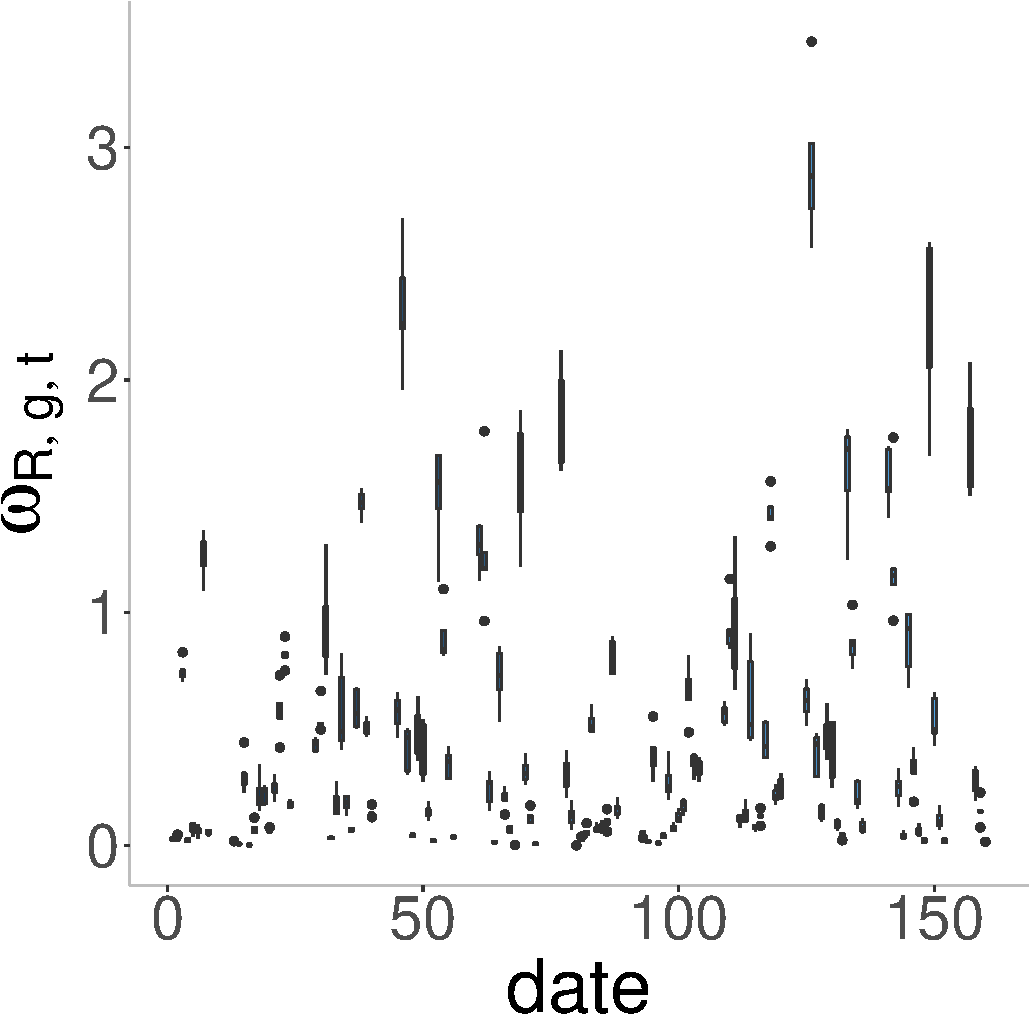
\includegraphics[width =5in, height =3in]{figs/weightsCPS78}
% Created by tikzDevice version 0.12.3.1 on 2023-11-03 10:48:14
% !TEX encoding = UTF-8 Unicode
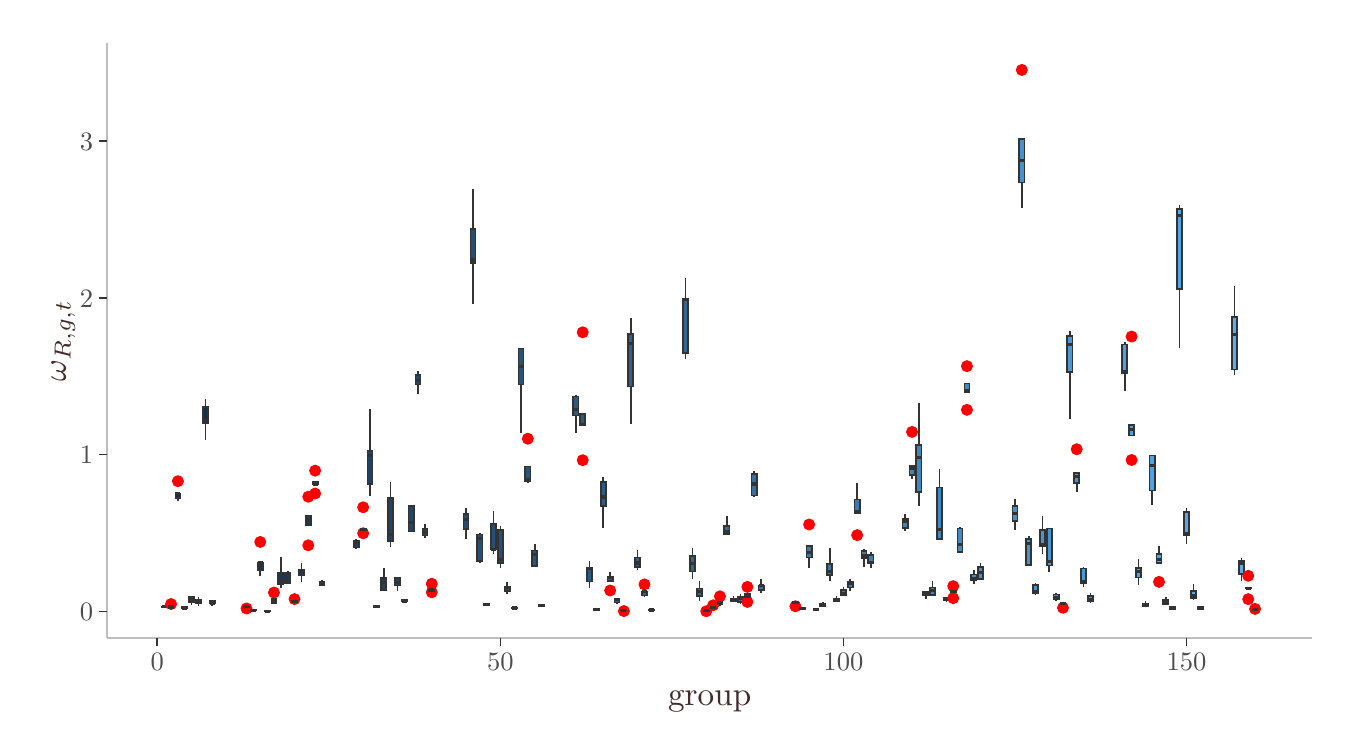
\begin{tikzpicture}[x=1pt,y=1pt]
\definecolor{fillColor}{RGB}{255,255,255}
\path[use as bounding box,fill=fillColor,fill opacity=0.00] (0,0) rectangle (469.75,252.94);
\begin{scope}
\path[clip] (  0.00,  0.00) rectangle (469.75,252.94);
\definecolor{drawColor}{RGB}{255,255,255}
\definecolor{fillColor}{RGB}{255,255,255}

\path[draw=drawColor,line width= 0.6pt,line join=round,line cap=round,fill=fillColor] (  0.00,  0.00) rectangle (469.76,252.94);
\end{scope}
\begin{scope}
\path[clip] ( 28.60, 32.28) rectangle (464.25,247.44);
\definecolor{drawColor}{RGB}{255,255,255}

\path[draw=drawColor,line width= 0.6pt,line join=round] ( 28.60, 42.02) --
	(464.25, 42.02);

\path[draw=drawColor,line width= 0.6pt,line join=round] ( 28.60, 98.66) --
	(464.25, 98.66);

\path[draw=drawColor,line width= 0.6pt,line join=round] ( 28.60,155.30) --
	(464.25,155.30);

\path[draw=drawColor,line width= 0.6pt,line join=round] ( 28.60,211.94) --
	(464.25,211.94);

\path[draw=drawColor,line width= 0.6pt,line join=round] ( 46.85, 32.28) --
	( 46.85,247.44);

\path[draw=drawColor,line width= 0.6pt,line join=round] (170.81, 32.28) --
	(170.81,247.44);

\path[draw=drawColor,line width= 0.6pt,line join=round] (294.77, 32.28) --
	(294.77,247.44);

\path[draw=drawColor,line width= 0.6pt,line join=round] (418.73, 32.28) --
	(418.73,247.44);
\definecolor{drawColor}{gray}{0.20}

\path[draw=drawColor,line width= 0.6pt,line join=round] ( 49.33, 43.82) -- ( 49.33, 44.17);

\path[draw=drawColor,line width= 0.6pt,line join=round] ( 49.33, 43.56) -- ( 49.33, 43.24);
\definecolor{fillColor}{RGB}{19,43,67}

\path[draw=drawColor,line width= 0.6pt,fill=fillColor] ( 48.40, 43.82) --
	( 48.40, 43.56) --
	( 50.26, 43.56) --
	( 50.26, 43.82) --
	( 48.40, 43.82) --
	cycle;

\path[draw=drawColor,line width= 1.1pt] ( 48.40, 43.62) -- ( 50.26, 43.62);
\definecolor{drawColor}{RGB}{255,0,0}
\definecolor{fillColor}{RGB}{255,0,0}

\path[draw=drawColor,line width= 0.4pt,line join=round,line cap=round,fill=fillColor] ( 51.81, 44.68) circle (  1.96);
\definecolor{drawColor}{gray}{0.20}

\path[draw=drawColor,line width= 0.6pt,line join=round] ( 51.81, 43.93) -- ( 51.81, 43.93);

\path[draw=drawColor,line width= 0.6pt,line join=round] ( 51.81, 43.46) -- ( 51.81, 43.08);
\definecolor{fillColor}{RGB}{19,44,68}

\path[draw=drawColor,line width= 0.6pt,fill=fillColor] ( 50.88, 43.93) --
	( 50.88, 43.46) --
	( 52.74, 43.46) --
	( 52.74, 43.93) --
	( 50.88, 43.93) --
	cycle;

\path[draw=drawColor,line width= 1.1pt] ( 50.88, 43.57) -- ( 52.74, 43.57);
\definecolor{drawColor}{RGB}{255,0,0}
\definecolor{fillColor}{RGB}{255,0,0}

\path[draw=drawColor,line width= 0.4pt,line join=round,line cap=round,fill=fillColor] ( 54.29, 89.06) circle (  1.96);
\definecolor{drawColor}{gray}{0.20}

\path[draw=drawColor,line width= 0.6pt,line join=round] ( 54.29, 84.51) -- ( 54.29, 84.51);

\path[draw=drawColor,line width= 0.6pt,line join=round] ( 54.29, 83.09) -- ( 54.29, 82.05);
\definecolor{fillColor}{RGB}{20,44,69}

\path[draw=drawColor,line width= 0.6pt,fill=fillColor] ( 53.36, 84.51) --
	( 53.36, 83.09) --
	( 55.22, 83.09) --
	( 55.22, 84.51) --
	( 53.36, 84.51) --
	cycle;

\path[draw=drawColor,line width= 1.1pt] ( 53.36, 84.46) -- ( 55.22, 84.46);

\path[draw=drawColor,line width= 0.6pt,line join=round] ( 56.77, 43.62) -- ( 56.77, 43.84);

\path[draw=drawColor,line width= 0.6pt,line join=round] ( 56.77, 43.00) -- ( 56.77, 42.97);
\definecolor{fillColor}{RGB}{20,45,70}

\path[draw=drawColor,line width= 0.6pt,fill=fillColor] ( 55.84, 43.62) --
	( 55.84, 43.00) --
	( 57.70, 43.00) --
	( 57.70, 43.62) --
	( 55.84, 43.62) --
	cycle;

\path[draw=drawColor,line width= 1.1pt] ( 55.84, 43.23) -- ( 57.70, 43.23);

\path[draw=drawColor,line width= 0.6pt,line join=round] ( 59.25, 47.27) -- ( 59.25, 47.51);

\path[draw=drawColor,line width= 0.6pt,line join=round] ( 59.25, 45.47) -- ( 59.25, 44.32);
\definecolor{fillColor}{RGB}{20,46,71}

\path[draw=drawColor,line width= 0.6pt,fill=fillColor] ( 58.32, 47.27) --
	( 58.32, 45.47) --
	( 60.18, 45.47) --
	( 60.18, 47.27) --
	( 58.32, 47.27) --
	cycle;

\path[draw=drawColor,line width= 1.1pt] ( 58.32, 46.40) -- ( 60.18, 46.40);

\path[draw=drawColor,line width= 0.6pt,line join=round] ( 61.72, 46.11) -- ( 61.72, 47.23);

\path[draw=drawColor,line width= 0.6pt,line join=round] ( 61.72, 45.12) -- ( 61.72, 43.83);
\definecolor{fillColor}{RGB}{21,47,72}

\path[draw=drawColor,line width= 0.6pt,fill=fillColor] ( 60.79, 46.11) --
	( 60.79, 45.12) --
	( 62.65, 45.12) --
	( 62.65, 46.11) --
	( 60.79, 46.11) --
	cycle;

\path[draw=drawColor,line width= 1.1pt] ( 60.79, 45.51) -- ( 62.65, 45.51);

\path[draw=drawColor,line width= 0.6pt,line join=round] ( 64.20,115.87) -- ( 64.20,118.59);

\path[draw=drawColor,line width= 0.6pt,line join=round] ( 64.20,110.16) -- ( 64.20,104.04);
\definecolor{fillColor}{RGB}{21,47,73}

\path[draw=drawColor,line width= 0.6pt,fill=fillColor] ( 63.27,115.87) --
	( 63.27,110.16) --
	( 65.13,110.16) --
	( 65.13,115.87) --
	( 63.27,115.87) --
	cycle;

\path[draw=drawColor,line width= 1.1pt] ( 63.27,111.08) -- ( 65.13,111.08);

\path[draw=drawColor,line width= 0.6pt,line join=round] ( 66.68, 45.66) -- ( 66.68, 45.72);

\path[draw=drawColor,line width= 0.6pt,line join=round] ( 66.68, 44.88) -- ( 66.68, 44.14);
\definecolor{fillColor}{RGB}{22,48,74}

\path[draw=drawColor,line width= 0.6pt,fill=fillColor] ( 65.75, 45.66) --
	( 65.75, 44.88) --
	( 67.61, 44.88) --
	( 67.61, 45.66) --
	( 65.75, 45.66) --
	cycle;

\path[draw=drawColor,line width= 1.1pt] ( 65.75, 45.02) -- ( 67.61, 45.02);
\definecolor{drawColor}{RGB}{255,0,0}
\definecolor{fillColor}{RGB}{255,0,0}

\path[draw=drawColor,line width= 0.4pt,line join=round,line cap=round,fill=fillColor] ( 79.08, 43.07) circle (  1.96);
\definecolor{drawColor}{gray}{0.20}

\path[draw=drawColor,line width= 0.6pt,line join=round] ( 79.08, 43.71) -- ( 79.08, 43.80);

\path[draw=drawColor,line width= 0.6pt,line join=round] ( 79.08, 43.60) -- ( 79.08, 43.60);
\definecolor{fillColor}{RGB}{24,52,79}

\path[draw=drawColor,line width= 0.6pt,fill=fillColor] ( 78.15, 43.71) --
	( 78.15, 43.60) --
	( 80.01, 43.60) --
	( 80.01, 43.71) --
	( 78.15, 43.71) --
	cycle;

\path[draw=drawColor,line width= 1.1pt] ( 78.15, 43.66) -- ( 80.01, 43.66);

\path[draw=drawColor,line width= 0.6pt,line join=round] ( 81.56, 42.49) -- ( 81.56, 42.62);

\path[draw=drawColor,line width= 0.6pt,line join=round] ( 81.56, 42.37) -- ( 81.56, 42.35);
\definecolor{fillColor}{RGB}{24,53,80}

\path[draw=drawColor,line width= 0.6pt,fill=fillColor] ( 80.63, 42.49) --
	( 80.63, 42.37) --
	( 82.49, 42.37) --
	( 82.49, 42.49) --
	( 80.63, 42.49) --
	cycle;

\path[draw=drawColor,line width= 1.1pt] ( 80.63, 42.42) -- ( 82.49, 42.42);
\definecolor{drawColor}{RGB}{255,0,0}
\definecolor{fillColor}{RGB}{255,0,0}

\path[draw=drawColor,line width= 0.4pt,line join=round,line cap=round,fill=fillColor] ( 84.04, 67.11) circle (  1.96);
\definecolor{drawColor}{gray}{0.20}

\path[draw=drawColor,line width= 0.6pt,line join=round] ( 84.04, 59.55) -- ( 84.04, 59.55);

\path[draw=drawColor,line width= 0.6pt,line join=round] ( 84.04, 56.90) -- ( 84.04, 54.95);
\definecolor{fillColor}{RGB}{24,53,81}

\path[draw=drawColor,line width= 0.6pt,fill=fillColor] ( 83.11, 59.55) --
	( 83.11, 56.90) --
	( 84.97, 56.90) --
	( 84.97, 59.55) --
	( 83.11, 59.55) --
	cycle;

\path[draw=drawColor,line width= 1.1pt] ( 83.11, 59.51) -- ( 84.97, 59.51);

\path[draw=drawColor,line width= 0.6pt,line join=round] ( 86.52, 42.15) -- ( 86.52, 42.19);

\path[draw=drawColor,line width= 0.6pt,line join=round] ( 86.52, 42.10) -- ( 86.52, 42.10);
\definecolor{fillColor}{RGB}{25,54,82}

\path[draw=drawColor,line width= 0.6pt,fill=fillColor] ( 85.59, 42.15) --
	( 85.59, 42.10) --
	( 87.45, 42.10) --
	( 87.45, 42.15) --
	( 85.59, 42.15) --
	cycle;

\path[draw=drawColor,line width= 1.1pt] ( 85.59, 42.13) -- ( 87.45, 42.13);
\definecolor{drawColor}{RGB}{255,0,0}
\definecolor{fillColor}{RGB}{255,0,0}

\path[draw=drawColor,line width= 0.4pt,line join=round,line cap=round,fill=fillColor] ( 89.00, 48.81) circle (  1.96);
\definecolor{drawColor}{gray}{0.20}

\path[draw=drawColor,line width= 0.6pt,line join=round] ( 89.00, 46.46) -- ( 89.00, 46.46);

\path[draw=drawColor,line width= 0.6pt,line join=round] ( 89.00, 45.13) -- ( 89.00, 44.85);
\definecolor{fillColor}{RGB}{25,55,83}

\path[draw=drawColor,line width= 0.6pt,fill=fillColor] ( 88.07, 46.46) --
	( 88.07, 45.13) --
	( 89.93, 45.13) --
	( 89.93, 46.46) --
	( 88.07, 46.46) --
	cycle;

\path[draw=drawColor,line width= 1.1pt] ( 88.07, 45.68) -- ( 89.93, 45.68);

\path[draw=drawColor,line width= 0.6pt,line join=round] ( 91.48, 55.94) -- ( 91.48, 61.73);

\path[draw=drawColor,line width= 0.6pt,line join=round] ( 91.48, 52.00) -- ( 91.48, 50.53);
\definecolor{fillColor}{RGB}{25,56,84}

\path[draw=drawColor,line width= 0.6pt,fill=fillColor] ( 90.55, 55.94) --
	( 90.55, 52.00) --
	( 92.40, 52.00) --
	( 92.40, 55.94) --
	( 90.55, 55.94) --
	cycle;

\path[draw=drawColor,line width= 1.1pt] ( 90.55, 53.29) -- ( 92.40, 53.29);

\path[draw=drawColor,line width= 0.6pt,line join=round] ( 93.95, 55.86) -- ( 93.95, 56.63);

\path[draw=drawColor,line width= 0.6pt,line join=round] ( 93.95, 52.19) -- ( 93.95, 51.80);
\definecolor{fillColor}{RGB}{26,56,85}

\path[draw=drawColor,line width= 0.6pt,fill=fillColor] ( 93.02, 55.86) --
	( 93.02, 52.19) --
	( 94.88, 52.19) --
	( 94.88, 55.86) --
	( 93.02, 55.86) --
	cycle;

\path[draw=drawColor,line width= 1.1pt] ( 93.02, 55.58) -- ( 94.88, 55.58);
\definecolor{drawColor}{RGB}{255,0,0}
\definecolor{fillColor}{RGB}{255,0,0}

\path[draw=drawColor,line width= 0.4pt,line join=round,line cap=round,fill=fillColor] ( 96.43, 46.45) circle (  1.96);
\definecolor{drawColor}{gray}{0.20}

\path[draw=drawColor,line width= 0.6pt,line join=round] ( 96.43, 45.65) -- ( 96.43, 45.65);

\path[draw=drawColor,line width= 0.6pt,line join=round] ( 96.43, 45.44) -- ( 96.43, 45.39);
\definecolor{fillColor}{RGB}{26,57,86}

\path[draw=drawColor,line width= 0.6pt,fill=fillColor] ( 95.50, 45.65) --
	( 95.50, 45.44) --
	( 97.36, 45.44) --
	( 97.36, 45.65) --
	( 95.50, 45.65) --
	cycle;

\path[draw=drawColor,line width= 1.1pt] ( 95.50, 45.58) -- ( 97.36, 45.58);

\path[draw=drawColor,line width= 0.6pt,line join=round] ( 98.91, 56.96) -- ( 98.91, 59.42);

\path[draw=drawColor,line width= 0.6pt,line join=round] ( 98.91, 54.98) -- ( 98.91, 52.73);
\definecolor{fillColor}{RGB}{27,58,87}

\path[draw=drawColor,line width= 0.6pt,fill=fillColor] ( 97.98, 56.96) --
	( 97.98, 54.98) --
	( 99.84, 54.98) --
	( 99.84, 56.96) --
	( 97.98, 56.96) --
	cycle;

\path[draw=drawColor,line width= 1.1pt] ( 97.98, 56.81) -- ( 99.84, 56.81);
\definecolor{drawColor}{RGB}{255,0,0}
\definecolor{fillColor}{RGB}{255,0,0}

\path[draw=drawColor,line width= 0.4pt,line join=round,line cap=round,fill=fillColor] (101.39, 65.89) circle (  1.96);

\path[draw=drawColor,line width= 0.4pt,line join=round,line cap=round,fill=fillColor] (101.39, 83.45) circle (  1.96);
\definecolor{drawColor}{gray}{0.20}

\path[draw=drawColor,line width= 0.6pt,line join=round] (101.39, 76.67) -- (101.39, 76.67);

\path[draw=drawColor,line width= 0.6pt,line join=round] (101.39, 73.07) -- (101.39, 73.07);
\definecolor{fillColor}{RGB}{27,59,88}

\path[draw=drawColor,line width= 0.6pt,fill=fillColor] (100.46, 76.67) --
	(100.46, 73.07) --
	(102.32, 73.07) --
	(102.32, 76.67) --
	(100.46, 76.67) --
	cycle;

\path[draw=drawColor,line width= 1.1pt] (100.46, 75.05) -- (102.32, 75.05);
\definecolor{drawColor}{RGB}{255,0,0}
\definecolor{fillColor}{RGB}{255,0,0}

\path[draw=drawColor,line width= 0.4pt,line join=round,line cap=round,fill=fillColor] (103.87, 92.86) circle (  1.96);

\path[draw=drawColor,line width= 0.4pt,line join=round,line cap=round,fill=fillColor] (103.87, 84.60) circle (  1.96);
\definecolor{drawColor}{gray}{0.20}

\path[draw=drawColor,line width= 0.6pt,line join=round] (103.87, 89.00) -- (103.87, 89.00);

\path[draw=drawColor,line width= 0.6pt,line join=round] (103.87, 87.83) -- (103.87, 87.83);
\definecolor{fillColor}{RGB}{27,60,89}

\path[draw=drawColor,line width= 0.6pt,fill=fillColor] (102.94, 89.00) --
	(102.94, 87.83) --
	(104.80, 87.83) --
	(104.80, 89.00) --
	(102.94, 89.00) --
	cycle;

\path[draw=drawColor,line width= 1.1pt] (102.94, 87.98) -- (104.80, 87.98);

\path[draw=drawColor,line width= 0.6pt,line join=round] (106.35, 52.56) -- (106.35, 53.33);

\path[draw=drawColor,line width= 0.6pt,line join=round] (106.35, 51.38) -- (106.35, 51.10);
\definecolor{fillColor}{RGB}{28,60,90}

\path[draw=drawColor,line width= 0.6pt,fill=fillColor] (105.42, 52.56) --
	(105.42, 51.38) --
	(107.28, 51.38) --
	(107.28, 52.56) --
	(105.42, 52.56) --
	cycle;

\path[draw=drawColor,line width= 1.1pt] (105.42, 51.57) -- (107.28, 51.57);

\path[draw=drawColor,line width= 0.6pt,line join=round] (118.75, 67.61) -- (118.75, 68.31);

\path[draw=drawColor,line width= 0.6pt,line join=round] (118.75, 65.05) -- (118.75, 64.64);
\definecolor{fillColor}{RGB}{30,64,96}

\path[draw=drawColor,line width= 0.6pt,fill=fillColor] (117.82, 67.61) --
	(117.82, 65.05) --
	(119.68, 65.05) --
	(119.68, 67.61) --
	(117.82, 67.61) --
	cycle;

\path[draw=drawColor,line width= 1.1pt] (117.82, 66.98) -- (119.68, 66.98);
\definecolor{drawColor}{RGB}{255,0,0}
\definecolor{fillColor}{RGB}{255,0,0}

\path[draw=drawColor,line width= 0.4pt,line join=round,line cap=round,fill=fillColor] (121.23, 79.63) circle (  1.96);

\path[draw=drawColor,line width= 0.4pt,line join=round,line cap=round,fill=fillColor] (121.23, 70.25) circle (  1.96);
\definecolor{drawColor}{gray}{0.20}

\path[draw=drawColor,line width= 0.6pt,line join=round] (121.23, 71.73) -- (121.23, 71.73);

\path[draw=drawColor,line width= 0.6pt,line join=round] (121.23, 71.30) -- (121.23, 71.30);
\definecolor{fillColor}{RGB}{30,65,97}

\path[draw=drawColor,line width= 0.6pt,fill=fillColor] (120.30, 71.73) --
	(120.30, 71.30) --
	(122.16, 71.30) --
	(122.16, 71.73) --
	(120.30, 71.73) --
	cycle;

\path[draw=drawColor,line width= 1.1pt] (120.30, 71.53) -- (122.16, 71.53);

\path[draw=drawColor,line width= 0.6pt,line join=round] (123.70,100.11) -- (123.70,115.24);

\path[draw=drawColor,line width= 0.6pt,line join=round] (123.70, 88.11) -- (123.70, 83.70);
\definecolor{fillColor}{RGB}{31,66,98}

\path[draw=drawColor,line width= 0.6pt,fill=fillColor] (122.78,100.11) --
	(122.78, 88.11) --
	(124.63, 88.11) --
	(124.63,100.11) --
	(122.78,100.11) --
	cycle;

\path[draw=drawColor,line width= 1.1pt] (122.78, 98.28) -- (124.63, 98.28);

\path[draw=drawColor,line width= 0.6pt,line join=round] (126.18, 44.04) -- (126.18, 44.06);

\path[draw=drawColor,line width= 0.6pt,line join=round] (126.18, 43.65) -- (126.18, 43.48);
\definecolor{fillColor}{RGB}{31,67,99}

\path[draw=drawColor,line width= 0.6pt,fill=fillColor] (125.25, 44.04) --
	(125.25, 43.65) --
	(127.11, 43.65) --
	(127.11, 44.04) --
	(125.25, 44.04) --
	cycle;

\path[draw=drawColor,line width= 1.1pt] (125.25, 43.93) -- (127.11, 43.93);

\path[draw=drawColor,line width= 0.6pt,line join=round] (128.66, 53.96) -- (128.66, 57.72);

\path[draw=drawColor,line width= 0.6pt,line join=round] (128.66, 49.79) -- (128.66, 49.57);
\definecolor{fillColor}{RGB}{31,67,100}

\path[draw=drawColor,line width= 0.6pt,fill=fillColor] (127.73, 53.96) --
	(127.73, 49.79) --
	(129.59, 49.79) --
	(129.59, 53.96) --
	(127.73, 53.96) --
	cycle;

\path[draw=drawColor,line width= 1.1pt] (127.73, 52.59) -- (129.59, 52.59);

\path[draw=drawColor,line width= 0.6pt,line join=round] (131.14, 82.92) -- (131.14, 88.76);

\path[draw=drawColor,line width= 0.6pt,line join=round] (131.14, 67.53) -- (131.14, 65.33);
\definecolor{fillColor}{RGB}{32,68,101}

\path[draw=drawColor,line width= 0.6pt,fill=fillColor] (130.21, 82.92) --
	(130.21, 67.53) --
	(132.07, 67.53) --
	(132.07, 82.92) --
	(130.21, 82.92) --
	cycle;

\path[draw=drawColor,line width= 1.1pt] (130.21, 69.72) -- (132.07, 69.72);

\path[draw=drawColor,line width= 0.6pt,line join=round] (133.62, 54.03) -- (133.62, 54.05);

\path[draw=drawColor,line width= 0.6pt,line join=round] (133.62, 51.31) -- (133.62, 49.34);
\definecolor{fillColor}{RGB}{32,69,102}

\path[draw=drawColor,line width= 0.6pt,fill=fillColor] (132.69, 54.03) --
	(132.69, 51.31) --
	(134.55, 51.31) --
	(134.55, 54.03) --
	(132.69, 54.03) --
	cycle;

\path[draw=drawColor,line width= 1.1pt] (132.69, 52.46) -- (134.55, 52.46);

\path[draw=drawColor,line width= 0.6pt,line join=round] (136.10, 46.17) -- (136.10, 46.23);

\path[draw=drawColor,line width= 0.6pt,line join=round] (136.10, 45.53) -- (136.10, 45.18);
\definecolor{fillColor}{RGB}{33,70,103}

\path[draw=drawColor,line width= 0.6pt,fill=fillColor] (135.17, 46.17) --
	(135.17, 45.53) --
	(137.03, 45.53) --
	(137.03, 46.17) --
	(135.17, 46.17) --
	cycle;

\path[draw=drawColor,line width= 1.1pt] (135.17, 45.69) -- (137.03, 45.69);

\path[draw=drawColor,line width= 0.6pt,line join=round] (138.58, 80.02) -- (138.58, 80.47);

\path[draw=drawColor,line width= 0.6pt,line join=round] (138.58, 70.94) -- (138.58, 70.58);
\definecolor{fillColor}{RGB}{33,70,104}

\path[draw=drawColor,line width= 0.6pt,fill=fillColor] (137.65, 80.02) --
	(137.65, 70.94) --
	(139.51, 70.94) --
	(139.51, 80.02) --
	(137.65, 80.02) --
	cycle;

\path[draw=drawColor,line width= 1.1pt] (137.65, 74.10) -- (139.51, 74.10);

\path[draw=drawColor,line width= 0.6pt,line join=round] (141.06,127.43) -- (141.06,129.00);

\path[draw=drawColor,line width= 0.6pt,line join=round] (141.06,124.00) -- (141.06,120.59);
\definecolor{fillColor}{RGB}{33,71,105}

\path[draw=drawColor,line width= 0.6pt,fill=fillColor] (140.13,127.43) --
	(140.13,124.00) --
	(141.99,124.00) --
	(141.99,127.43) --
	(140.13,127.43) --
	cycle;

\path[draw=drawColor,line width= 1.1pt] (140.13,125.53) -- (141.99,125.53);

\path[draw=drawColor,line width= 0.6pt,line join=round] (143.54, 71.85) -- (143.54, 73.54);

\path[draw=drawColor,line width= 0.6pt,line join=round] (143.54, 69.39) -- (143.54, 68.53);
\definecolor{fillColor}{RGB}{34,72,106}

\path[draw=drawColor,line width= 0.6pt,fill=fillColor] (142.61, 71.85) --
	(142.61, 69.39) --
	(144.47, 69.39) --
	(144.47, 71.85) --
	(142.61, 71.85) --
	cycle;

\path[draw=drawColor,line width= 1.1pt] (142.61, 70.64) -- (144.47, 70.64);
\definecolor{drawColor}{RGB}{255,0,0}
\definecolor{fillColor}{RGB}{255,0,0}

\path[draw=drawColor,line width= 0.4pt,line join=round,line cap=round,fill=fillColor] (146.02, 51.99) circle (  1.96);

\path[draw=drawColor,line width= 0.4pt,line join=round,line cap=round,fill=fillColor] (146.02, 48.91) circle (  1.96);
\definecolor{drawColor}{gray}{0.20}

\path[draw=drawColor,line width= 0.6pt,line join=round] (146.02, 49.87) -- (146.02, 49.87);

\path[draw=drawColor,line width= 0.6pt,line join=round] (146.02, 49.49) -- (146.02, 49.49);
\definecolor{fillColor}{RGB}{34,73,107}

\path[draw=drawColor,line width= 0.6pt,fill=fillColor] (145.09, 49.87) --
	(145.09, 49.49) --
	(146.95, 49.49) --
	(146.95, 49.87) --
	(145.09, 49.87) --
	cycle;

\path[draw=drawColor,line width= 1.1pt] (145.09, 49.82) -- (146.95, 49.82);

\path[draw=drawColor,line width= 0.6pt,line join=round] (158.41, 77.23) -- (158.41, 79.22);

\path[draw=drawColor,line width= 0.6pt,line join=round] (158.41, 71.77) -- (158.41, 68.23);
\definecolor{fillColor}{RGB}{36,77,113}

\path[draw=drawColor,line width= 0.6pt,fill=fillColor] (157.48, 77.23) --
	(157.48, 71.77) --
	(159.34, 71.77) --
	(159.34, 77.23) --
	(157.48, 77.23) --
	cycle;

\path[draw=drawColor,line width= 1.1pt] (157.48, 75.05) -- (159.34, 75.05);

\path[draw=drawColor,line width= 0.6pt,line join=round] (160.89,180.14) -- (160.89,194.56);

\path[draw=drawColor,line width= 0.6pt,line join=round] (160.89,167.79) -- (160.89,152.96);
\definecolor{fillColor}{RGB}{37,78,114}

\path[draw=drawColor,line width= 0.6pt,fill=fillColor] (159.96,180.14) --
	(159.96,167.79) --
	(161.82,167.79) --
	(161.82,180.14) --
	(159.96,180.14) --
	cycle;

\path[draw=drawColor,line width= 1.1pt] (159.96,168.98) -- (161.82,168.98);

\path[draw=drawColor,line width= 0.6pt,line join=round] (163.37, 69.75) -- (163.37, 70.42);

\path[draw=drawColor,line width= 0.6pt,line join=round] (163.37, 60.17) -- (163.37, 59.41);
\definecolor{fillColor}{RGB}{37,78,115}

\path[draw=drawColor,line width= 0.6pt,fill=fillColor] (162.44, 69.75) --
	(162.44, 60.17) --
	(164.30, 60.17) --
	(164.30, 69.75) --
	(162.44, 69.75) --
	cycle;

\path[draw=drawColor,line width= 1.1pt] (162.44, 68.26) -- (164.30, 68.26);

\path[draw=drawColor,line width= 0.6pt,line join=round] (165.85, 44.65) -- (165.85, 44.94);

\path[draw=drawColor,line width= 0.6pt,line join=round] (165.85, 44.23) -- (165.85, 43.98);
\definecolor{fillColor}{RGB}{37,79,116}

\path[draw=drawColor,line width= 0.6pt,fill=fillColor] (164.92, 44.65) --
	(164.92, 44.23) --
	(166.78, 44.23) --
	(166.78, 44.65) --
	(164.92, 44.65) --
	cycle;

\path[draw=drawColor,line width= 1.1pt] (164.92, 44.61) -- (166.78, 44.61);

\path[draw=drawColor,line width= 0.6pt,line join=round] (168.33, 73.57) -- (168.33, 78.30);

\path[draw=drawColor,line width= 0.6pt,line join=round] (168.33, 64.52) -- (168.33, 62.63);
\definecolor{fillColor}{RGB}{38,80,117}

\path[draw=drawColor,line width= 0.6pt,fill=fillColor] (167.40, 73.57) --
	(167.40, 64.52) --
	(169.26, 64.52) --
	(169.26, 73.57) --
	(167.40, 73.57) --
	cycle;

\path[draw=drawColor,line width= 1.1pt] (167.40, 64.52) -- (169.26, 64.52);

\path[draw=drawColor,line width= 0.6pt,line join=round] (170.81, 71.40) -- (170.81, 72.80);

\path[draw=drawColor,line width= 0.6pt,line join=round] (170.81, 59.40) -- (170.81, 57.70);
\definecolor{fillColor}{RGB}{38,81,118}

\path[draw=drawColor,line width= 0.6pt,fill=fillColor] (169.88, 71.40) --
	(169.88, 59.40) --
	(171.74, 59.40) --
	(171.74, 71.40) --
	(169.88, 71.40) --
	cycle;

\path[draw=drawColor,line width= 1.1pt] (169.88, 60.82) -- (171.74, 60.82);

\path[draw=drawColor,line width= 0.6pt,line join=round] (173.29, 50.79) -- (173.29, 52.68);

\path[draw=drawColor,line width= 0.6pt,line join=round] (173.29, 49.38) -- (173.29, 48.15);
\definecolor{fillColor}{RGB}{39,82,119}

\path[draw=drawColor,line width= 0.6pt,fill=fillColor] (172.36, 50.79) --
	(172.36, 49.38) --
	(174.22, 49.38) --
	(174.22, 50.79) --
	(172.36, 50.79) --
	cycle;

\path[draw=drawColor,line width= 1.1pt] (172.36, 50.65) -- (174.22, 50.65);

\path[draw=drawColor,line width= 0.6pt,line join=round] (175.77, 43.37) -- (175.77, 43.43);

\path[draw=drawColor,line width= 0.6pt,line join=round] (175.77, 43.03) -- (175.77, 42.79);
\definecolor{fillColor}{RGB}{39,82,120}

\path[draw=drawColor,line width= 0.6pt,fill=fillColor] (174.84, 43.37) --
	(174.84, 43.03) --
	(176.70, 43.03) --
	(176.70, 43.37) --
	(174.84, 43.37) --
	cycle;

\path[draw=drawColor,line width= 1.1pt] (174.84, 43.24) -- (176.70, 43.24);

\path[draw=drawColor,line width= 0.6pt,line join=round] (178.25,136.95) -- (178.25,137.02);

\path[draw=drawColor,line width= 0.6pt,line join=round] (178.25,123.99) -- (178.25,106.31);
\definecolor{fillColor}{RGB}{39,83,121}

\path[draw=drawColor,line width= 0.6pt,fill=fillColor] (177.32,136.95) --
	(177.32,123.99) --
	(179.18,123.99) --
	(179.18,136.95) --
	(177.32,136.95) --
	cycle;

\path[draw=drawColor,line width= 1.1pt] (177.32,130.45) -- (179.18,130.45);
\definecolor{drawColor}{RGB}{255,0,0}
\definecolor{fillColor}{RGB}{255,0,0}

\path[draw=drawColor,line width= 0.4pt,line join=round,line cap=round,fill=fillColor] (180.73,104.41) circle (  1.96);
\definecolor{drawColor}{gray}{0.20}

\path[draw=drawColor,line width= 0.6pt,line join=round] (180.73, 94.34) -- (180.73, 94.34);

\path[draw=drawColor,line width= 0.6pt,line join=round] (180.73, 88.93) -- (180.73, 88.31);
\definecolor{fillColor}{RGB}{40,84,122}

\path[draw=drawColor,line width= 0.6pt,fill=fillColor] (179.80, 94.34) --
	(179.80, 88.93) --
	(181.66, 88.93) --
	(181.66, 94.34) --
	(179.80, 94.34) --
	cycle;

\path[draw=drawColor,line width= 1.1pt] (179.80, 89.59) -- (181.66, 89.59);

\path[draw=drawColor,line width= 0.6pt,line join=round] (183.21, 63.98) -- (183.21, 66.23);

\path[draw=drawColor,line width= 0.6pt,line join=round] (183.21, 58.32) -- (183.21, 58.19);
\definecolor{fillColor}{RGB}{40,85,123}

\path[draw=drawColor,line width= 0.6pt,fill=fillColor] (182.28, 63.98) --
	(182.28, 58.32) --
	(184.14, 58.32) --
	(184.14, 63.98) --
	(182.28, 63.98) --
	cycle;

\path[draw=drawColor,line width= 1.1pt] (182.28, 62.52) -- (184.14, 62.52);

\path[draw=drawColor,line width= 0.6pt,line join=round] (185.69, 44.25) -- (185.69, 44.30);

\path[draw=drawColor,line width= 0.6pt,line join=round] (185.69, 44.03) -- (185.69, 43.70);
\definecolor{fillColor}{RGB}{41,86,125}

\path[draw=drawColor,line width= 0.6pt,fill=fillColor] (184.76, 44.25) --
	(184.76, 44.03) --
	(186.61, 44.03) --
	(186.61, 44.25) --
	(184.76, 44.25) --
	cycle;

\path[draw=drawColor,line width= 1.1pt] (184.76, 44.09) -- (186.61, 44.09);

\path[draw=drawColor,line width= 0.6pt,line join=round] (198.08,119.70) -- (198.08,120.06);

\path[draw=drawColor,line width= 0.6pt,line join=round] (198.08,112.77) -- (198.08,106.53);
\definecolor{fillColor}{RGB}{43,90,130}

\path[draw=drawColor,line width= 0.6pt,fill=fillColor] (197.15,119.70) --
	(197.15,112.77) --
	(199.01,112.77) --
	(199.01,119.70) --
	(197.15,119.70) --
	cycle;

\path[draw=drawColor,line width= 1.1pt] (197.15,115.13) -- (199.01,115.13);
\definecolor{drawColor}{RGB}{255,0,0}
\definecolor{fillColor}{RGB}{255,0,0}

\path[draw=drawColor,line width= 0.4pt,line join=round,line cap=round,fill=fillColor] (200.56,142.86) circle (  1.96);

\path[draw=drawColor,line width= 0.4pt,line join=round,line cap=round,fill=fillColor] (200.56, 96.65) circle (  1.96);
\definecolor{drawColor}{gray}{0.20}

\path[draw=drawColor,line width= 0.6pt,line join=round] (200.56,113.34) -- (200.56,113.34);

\path[draw=drawColor,line width= 0.6pt,line join=round] (200.56,109.27) -- (200.56,109.27);
\definecolor{fillColor}{RGB}{43,91,131}

\path[draw=drawColor,line width= 0.6pt,fill=fillColor] (199.63,113.34) --
	(199.63,109.27) --
	(201.49,109.27) --
	(201.49,113.34) --
	(199.63,113.34) --
	cycle;

\path[draw=drawColor,line width= 1.1pt] (199.63,109.48) -- (201.49,109.48);

\path[draw=drawColor,line width= 0.6pt,line join=round] (203.04, 57.62) -- (203.04, 60.15);

\path[draw=drawColor,line width= 0.6pt,line join=round] (203.04, 52.83) -- (203.04, 50.44);
\definecolor{fillColor}{RGB}{43,91,132}

\path[draw=drawColor,line width= 0.6pt,fill=fillColor] (202.11, 57.62) --
	(202.11, 52.83) --
	(203.97, 52.83) --
	(203.97, 57.62) --
	(202.11, 57.62) --
	cycle;

\path[draw=drawColor,line width= 1.1pt] (202.11, 57.35) -- (203.97, 57.35);

\path[draw=drawColor,line width= 0.6pt,line join=round] (205.52, 42.92) -- (205.52, 42.96);

\path[draw=drawColor,line width= 0.6pt,line join=round] (205.52, 42.63) -- (205.52, 42.35);
\definecolor{fillColor}{RGB}{44,92,133}

\path[draw=drawColor,line width= 0.6pt,fill=fillColor] (204.59, 42.92) --
	(204.59, 42.63) --
	(206.45, 42.63) --
	(206.45, 42.92) --
	(204.59, 42.92) --
	cycle;

\path[draw=drawColor,line width= 1.1pt] (204.59, 42.75) -- (206.45, 42.75);

\path[draw=drawColor,line width= 0.6pt,line join=round] (208.00, 88.77) -- (208.00, 90.42);

\path[draw=drawColor,line width= 0.6pt,line join=round] (208.00, 80.05) -- (208.00, 72.13);
\definecolor{fillColor}{RGB}{44,93,134}

\path[draw=drawColor,line width= 0.6pt,fill=fillColor] (207.07, 88.77) --
	(207.07, 80.05) --
	(208.93, 80.05) --
	(208.93, 88.77) --
	(207.07, 88.77) --
	cycle;

\path[draw=drawColor,line width= 1.1pt] (207.07, 83.34) -- (208.93, 83.34);
\definecolor{drawColor}{RGB}{255,0,0}
\definecolor{fillColor}{RGB}{255,0,0}

\path[draw=drawColor,line width= 0.4pt,line join=round,line cap=round,fill=fillColor] (210.48, 49.57) circle (  1.96);
\definecolor{drawColor}{gray}{0.20}

\path[draw=drawColor,line width= 0.6pt,line join=round] (210.48, 54.62) -- (210.48, 56.35);

\path[draw=drawColor,line width= 0.6pt,line join=round] (210.48, 53.07) -- (210.48, 53.07);
\definecolor{fillColor}{RGB}{45,94,136}

\path[draw=drawColor,line width= 0.6pt,fill=fillColor] (209.55, 54.62) --
	(209.55, 53.07) --
	(211.41, 53.07) --
	(211.41, 54.62) --
	(209.55, 54.62) --
	cycle;

\path[draw=drawColor,line width= 1.1pt] (209.55, 54.42) -- (211.41, 54.42);

\path[draw=drawColor,line width= 0.6pt,line join=round] (212.96, 46.58) -- (212.96, 46.66);

\path[draw=drawColor,line width= 0.6pt,line join=round] (212.96, 45.21) -- (212.96, 45.07);
\definecolor{fillColor}{RGB}{45,95,137}

\path[draw=drawColor,line width= 0.6pt,fill=fillColor] (212.03, 46.58) --
	(212.03, 45.21) --
	(213.89, 45.21) --
	(213.89, 46.58) --
	(212.03, 46.58) --
	cycle;

\path[draw=drawColor,line width= 1.1pt] (212.03, 46.18) -- (213.89, 46.18);
\definecolor{drawColor}{RGB}{255,0,0}
\definecolor{fillColor}{RGB}{255,0,0}

\path[draw=drawColor,line width= 0.4pt,line join=round,line cap=round,fill=fillColor] (215.44, 42.12) circle (  1.96);
\definecolor{drawColor}{gray}{0.20}

\path[draw=drawColor,line width= 0.6pt,line join=round] (215.44, 42.37) -- (215.44, 42.38);

\path[draw=drawColor,line width= 0.6pt,line join=round] (215.44, 42.33) -- (215.44, 42.33);
\definecolor{fillColor}{RGB}{46,96,138}

\path[draw=drawColor,line width= 0.6pt,fill=fillColor] (214.51, 42.37) --
	(214.51, 42.33) --
	(216.37, 42.33) --
	(216.37, 42.37) --
	(214.51, 42.37) --
	cycle;

\path[draw=drawColor,line width= 1.1pt] (214.51, 42.34) -- (216.37, 42.34);

\path[draw=drawColor,line width= 0.6pt,line join=round] (217.91,142.25) -- (217.91,147.93);

\path[draw=drawColor,line width= 0.6pt,line join=round] (217.91,123.24) -- (217.91,109.88);
\definecolor{fillColor}{RGB}{46,96,139}

\path[draw=drawColor,line width= 0.6pt,fill=fillColor] (216.99,142.25) --
	(216.99,123.24) --
	(218.84,123.24) --
	(218.84,142.25) --
	(216.99,142.25) --
	cycle;

\path[draw=drawColor,line width= 1.1pt] (216.99,138.70) -- (218.84,138.70);

\path[draw=drawColor,line width= 0.6pt,line join=round] (220.39, 61.51) -- (220.39, 64.34);

\path[draw=drawColor,line width= 0.6pt,line join=round] (220.39, 58.17) -- (220.39, 56.84);
\definecolor{fillColor}{RGB}{46,97,140}

\path[draw=drawColor,line width= 0.6pt,fill=fillColor] (219.46, 61.51) --
	(219.46, 58.17) --
	(221.32, 58.17) --
	(221.32, 61.51) --
	(219.46, 61.51) --
	cycle;

\path[draw=drawColor,line width= 1.1pt] (219.46, 59.50) -- (221.32, 59.50);
\definecolor{drawColor}{RGB}{255,0,0}
\definecolor{fillColor}{RGB}{255,0,0}

\path[draw=drawColor,line width= 0.4pt,line join=round,line cap=round,fill=fillColor] (222.87, 51.76) circle (  1.96);
\definecolor{drawColor}{gray}{0.20}

\path[draw=drawColor,line width= 0.6pt,line join=round] (222.87, 49.23) -- (222.87, 49.23);

\path[draw=drawColor,line width= 0.6pt,line join=round] (222.87, 47.70) -- (222.87, 47.54);
\definecolor{fillColor}{RGB}{47,98,141}

\path[draw=drawColor,line width= 0.6pt,fill=fillColor] (221.94, 49.23) --
	(221.94, 47.70) --
	(223.80, 47.70) --
	(223.80, 49.23) --
	(221.94, 49.23) --
	cycle;

\path[draw=drawColor,line width= 1.1pt] (221.94, 49.09) -- (223.80, 49.09);

\path[draw=drawColor,line width= 0.6pt,line join=round] (225.35, 42.57) -- (225.35, 42.58);

\path[draw=drawColor,line width= 0.6pt,line join=round] (225.35, 42.33) -- (225.35, 42.29);
\definecolor{fillColor}{RGB}{47,99,142}

\path[draw=drawColor,line width= 0.6pt,fill=fillColor] (224.42, 42.57) --
	(224.42, 42.33) --
	(226.28, 42.33) --
	(226.28, 42.57) --
	(224.42, 42.57) --
	cycle;

\path[draw=drawColor,line width= 1.1pt] (224.42, 42.52) -- (226.28, 42.52);

\path[draw=drawColor,line width= 0.6pt,line join=round] (237.75,155.09) -- (237.75,162.58);

\path[draw=drawColor,line width= 0.6pt,line join=round] (237.75,135.30) -- (237.75,133.26);
\definecolor{fillColor}{RGB}{49,103,148}

\path[draw=drawColor,line width= 0.6pt,fill=fillColor] (236.82,155.09) --
	(236.82,135.30) --
	(238.68,135.30) --
	(238.68,155.09) --
	(236.82,155.09) --
	cycle;

\path[draw=drawColor,line width= 1.1pt] (236.82,154.70) -- (238.68,154.70);

\path[draw=drawColor,line width= 0.6pt,line join=round] (240.23, 62.08) -- (240.23, 65.04);

\path[draw=drawColor,line width= 0.6pt,line join=round] (240.23, 56.44) -- (240.23, 53.81);
\definecolor{fillColor}{RGB}{50,104,149}

\path[draw=drawColor,line width= 0.6pt,fill=fillColor] (239.30, 62.08) --
	(239.30, 56.44) --
	(241.16, 56.44) --
	(241.16, 62.08) --
	(239.30, 62.08) --
	cycle;

\path[draw=drawColor,line width= 1.1pt] (239.30, 59.33) -- (241.16, 59.33);

\path[draw=drawColor,line width= 0.6pt,line join=round] (242.71, 50.30) -- (242.71, 52.90);

\path[draw=drawColor,line width= 0.6pt,line join=round] (242.71, 47.63) -- (242.71, 45.87);
\definecolor{fillColor}{RGB}{50,105,150}

\path[draw=drawColor,line width= 0.6pt,fill=fillColor] (241.78, 50.30) --
	(241.78, 47.63) --
	(243.64, 47.63) --
	(243.64, 50.30) --
	(241.78, 50.30) --
	cycle;

\path[draw=drawColor,line width= 1.1pt] (241.78, 49.18) -- (243.64, 49.18);
\definecolor{drawColor}{RGB}{255,0,0}
\definecolor{fillColor}{RGB}{255,0,0}

\path[draw=drawColor,line width= 0.4pt,line join=round,line cap=round,fill=fillColor] (245.19, 42.06) circle (  1.96);
\definecolor{drawColor}{gray}{0.20}

\path[draw=drawColor,line width= 0.6pt,line join=round] (245.19, 42.24) -- (245.19, 42.26);

\path[draw=drawColor,line width= 0.6pt,line join=round] (245.19, 42.19) -- (245.19, 42.19);
\definecolor{fillColor}{RGB}{51,106,151}

\path[draw=drawColor,line width= 0.6pt,fill=fillColor] (244.26, 42.24) --
	(244.26, 42.19) --
	(246.12, 42.19) --
	(246.12, 42.24) --
	(244.26, 42.24) --
	cycle;

\path[draw=drawColor,line width= 1.1pt] (244.26, 42.21) -- (246.12, 42.21);
\definecolor{drawColor}{RGB}{255,0,0}
\definecolor{fillColor}{RGB}{255,0,0}

\path[draw=drawColor,line width= 0.4pt,line join=round,line cap=round,fill=fillColor] (247.67, 44.21) circle (  1.96);
\definecolor{drawColor}{gray}{0.20}

\path[draw=drawColor,line width= 0.6pt,line join=round] (247.67, 43.54) -- (247.67, 43.54);

\path[draw=drawColor,line width= 0.6pt,line join=round] (247.67, 43.22) -- (247.67, 43.16);
\definecolor{fillColor}{RGB}{51,107,153}

\path[draw=drawColor,line width= 0.6pt,fill=fillColor] (246.74, 43.54) --
	(246.74, 43.22) --
	(248.59, 43.22) --
	(248.59, 43.54) --
	(246.74, 43.54) --
	cycle;

\path[draw=drawColor,line width= 1.1pt] (246.74, 43.50) -- (248.59, 43.50);
\definecolor{drawColor}{RGB}{255,0,0}
\definecolor{fillColor}{RGB}{255,0,0}

\path[draw=drawColor,line width= 0.4pt,line join=round,line cap=round,fill=fillColor] (250.14, 47.46) circle (  1.96);
\definecolor{drawColor}{gray}{0.20}

\path[draw=drawColor,line width= 0.6pt,line join=round] (250.14, 45.53) -- (250.14, 45.53);

\path[draw=drawColor,line width= 0.6pt,line join=round] (250.14, 44.71) -- (250.14, 44.06);
\definecolor{fillColor}{RGB}{51,107,154}

\path[draw=drawColor,line width= 0.6pt,fill=fillColor] (249.21, 45.53) --
	(249.21, 44.71) --
	(251.07, 44.71) --
	(251.07, 45.53) --
	(249.21, 45.53) --
	cycle;

\path[draw=drawColor,line width= 1.1pt] (249.21, 45.25) -- (251.07, 45.25);

\path[draw=drawColor,line width= 0.6pt,line join=round] (252.62, 72.92) -- (252.62, 76.36);

\path[draw=drawColor,line width= 0.6pt,line join=round] (252.62, 69.89) -- (252.62, 69.45);
\definecolor{fillColor}{RGB}{52,108,155}

\path[draw=drawColor,line width= 0.6pt,fill=fillColor] (251.69, 72.92) --
	(251.69, 69.89) --
	(253.55, 69.89) --
	(253.55, 72.92) --
	(251.69, 72.92) --
	cycle;

\path[draw=drawColor,line width= 1.1pt] (251.69, 70.84) -- (253.55, 70.84);

\path[draw=drawColor,line width= 0.6pt,line join=round] (255.10, 46.38) -- (255.10, 47.55);

\path[draw=drawColor,line width= 0.6pt,line join=round] (255.10, 45.60) -- (255.10, 45.27);
\definecolor{fillColor}{RGB}{52,109,156}

\path[draw=drawColor,line width= 0.6pt,fill=fillColor] (254.17, 46.38) --
	(254.17, 45.60) --
	(256.03, 45.60) --
	(256.03, 46.38) --
	(254.17, 46.38) --
	cycle;

\path[draw=drawColor,line width= 1.1pt] (254.17, 45.79) -- (256.03, 45.79);

\path[draw=drawColor,line width= 0.6pt,line join=round] (257.58, 47.17) -- (257.58, 48.22);

\path[draw=drawColor,line width= 0.6pt,line join=round] (257.58, 45.36) -- (257.58, 44.85);
\definecolor{fillColor}{RGB}{53,110,157}

\path[draw=drawColor,line width= 0.6pt,fill=fillColor] (256.65, 47.17) --
	(256.65, 45.36) --
	(258.51, 45.36) --
	(258.51, 47.17) --
	(256.65, 47.17) --
	cycle;

\path[draw=drawColor,line width= 1.1pt] (256.65, 46.74) -- (258.51, 46.74);
\definecolor{drawColor}{RGB}{255,0,0}
\definecolor{fillColor}{RGB}{255,0,0}

\path[draw=drawColor,line width= 0.4pt,line join=round,line cap=round,fill=fillColor] (260.06, 45.44) circle (  1.96);

\path[draw=drawColor,line width= 0.4pt,line join=round,line cap=round,fill=fillColor] (260.06, 50.87) circle (  1.96);
\definecolor{drawColor}{gray}{0.20}

\path[draw=drawColor,line width= 0.6pt,line join=round] (260.06, 48.37) -- (260.06, 48.37);

\path[draw=drawColor,line width= 0.6pt,line join=round] (260.06, 47.26) -- (260.06, 47.26);
\definecolor{fillColor}{RGB}{53,111,158}

\path[draw=drawColor,line width= 0.6pt,fill=fillColor] (259.13, 48.37) --
	(259.13, 47.26) --
	(260.99, 47.26) --
	(260.99, 48.37) --
	(259.13, 48.37) --
	cycle;

\path[draw=drawColor,line width= 1.1pt] (259.13, 47.68) -- (260.99, 47.68);

\path[draw=drawColor,line width= 0.6pt,line join=round] (262.54, 91.56) -- (262.54, 92.87);

\path[draw=drawColor,line width= 0.6pt,line join=round] (262.54, 83.88) -- (262.54, 83.62);
\definecolor{fillColor}{RGB}{54,112,159}

\path[draw=drawColor,line width= 0.6pt,fill=fillColor] (261.61, 91.56) --
	(261.61, 83.88) --
	(263.47, 83.88) --
	(263.47, 91.56) --
	(261.61, 91.56) --
	cycle;

\path[draw=drawColor,line width= 1.1pt] (261.61, 88.05) -- (263.47, 88.05);

\path[draw=drawColor,line width= 0.6pt,line join=round] (265.02, 51.42) -- (265.02, 53.82);

\path[draw=drawColor,line width= 0.6pt,line join=round] (265.02, 49.69) -- (265.02, 48.61);
\definecolor{fillColor}{RGB}{54,113,161}

\path[draw=drawColor,line width= 0.6pt,fill=fillColor] (264.09, 51.42) --
	(264.09, 49.69) --
	(265.95, 49.69) --
	(265.95, 51.42) --
	(264.09, 51.42) --
	cycle;

\path[draw=drawColor,line width= 1.1pt] (264.09, 51.33) -- (265.95, 51.33);
\definecolor{drawColor}{RGB}{255,0,0}
\definecolor{fillColor}{RGB}{255,0,0}

\path[draw=drawColor,line width= 0.4pt,line join=round,line cap=round,fill=fillColor] (277.42, 43.86) circle (  1.96);
\definecolor{drawColor}{gray}{0.20}

\path[draw=drawColor,line width= 0.6pt,line join=round] (277.42, 45.35) -- (277.42, 45.38);

\path[draw=drawColor,line width= 0.6pt,line join=round] (277.42, 44.82) -- (277.42, 44.82);
\definecolor{fillColor}{RGB}{56,117,166}

\path[draw=drawColor,line width= 0.6pt,fill=fillColor] (276.49, 45.35) --
	(276.49, 44.82) --
	(278.35, 44.82) --
	(278.35, 45.35) --
	(276.49, 45.35) --
	cycle;

\path[draw=drawColor,line width= 1.1pt] (276.49, 45.12) -- (278.35, 45.12);

\path[draw=drawColor,line width= 0.6pt,line join=round] (279.89, 43.14) -- (279.89, 43.21);

\path[draw=drawColor,line width= 0.6pt,line join=round] (279.89, 42.87) -- (279.89, 42.79);
\definecolor{fillColor}{RGB}{57,118,167}

\path[draw=drawColor,line width= 0.6pt,fill=fillColor] (278.97, 43.14) --
	(278.97, 42.87) --
	(280.82, 42.87) --
	(280.82, 43.14) --
	(278.97, 43.14) --
	cycle;

\path[draw=drawColor,line width= 1.1pt] (278.97, 43.06) -- (280.82, 43.06);
\definecolor{drawColor}{RGB}{255,0,0}
\definecolor{fillColor}{RGB}{255,0,0}

\path[draw=drawColor,line width= 0.4pt,line join=round,line cap=round,fill=fillColor] (282.37, 73.41) circle (  1.96);
\definecolor{drawColor}{gray}{0.20}

\path[draw=drawColor,line width= 0.6pt,line join=round] (282.37, 65.76) -- (282.37, 65.76);

\path[draw=drawColor,line width= 0.6pt,line join=round] (282.37, 61.47) -- (282.37, 57.70);
\definecolor{fillColor}{RGB}{57,119,169}

\path[draw=drawColor,line width= 0.6pt,fill=fillColor] (281.44, 65.76) --
	(281.44, 61.47) --
	(283.30, 61.47) --
	(283.30, 65.76) --
	(281.44, 65.76) --
	cycle;

\path[draw=drawColor,line width= 1.1pt] (281.44, 63.12) -- (283.30, 63.12);

\path[draw=drawColor,line width= 0.6pt,line join=round] (284.85, 42.63) -- (284.85, 42.68);

\path[draw=drawColor,line width= 0.6pt,line join=round] (284.85, 42.54) -- (284.85, 42.42);
\definecolor{fillColor}{RGB}{57,119,170}

\path[draw=drawColor,line width= 0.6pt,fill=fillColor] (283.92, 42.63) --
	(283.92, 42.54) --
	(285.78, 42.54) --
	(285.78, 42.63) --
	(283.92, 42.63) --
	cycle;

\path[draw=drawColor,line width= 1.1pt] (283.92, 42.61) -- (285.78, 42.61);

\path[draw=drawColor,line width= 0.6pt,line join=round] (287.33, 44.62) -- (287.33, 45.31);

\path[draw=drawColor,line width= 0.6pt,line join=round] (287.33, 43.89) -- (287.33, 43.72);
\definecolor{fillColor}{RGB}{58,120,171}

\path[draw=drawColor,line width= 0.6pt,fill=fillColor] (286.40, 44.62) --
	(286.40, 43.89) --
	(288.26, 43.89) --
	(288.26, 44.62) --
	(286.40, 44.62) --
	cycle;

\path[draw=drawColor,line width= 1.1pt] (286.40, 44.62) -- (288.26, 44.62);

\path[draw=drawColor,line width= 0.6pt,line join=round] (289.81, 59.10) -- (289.81, 64.95);

\path[draw=drawColor,line width= 0.6pt,line join=round] (289.81, 55.19) -- (289.81, 53.16);
\definecolor{fillColor}{RGB}{58,121,172}

\path[draw=drawColor,line width= 0.6pt,fill=fillColor] (288.88, 59.10) --
	(288.88, 55.19) --
	(290.74, 55.19) --
	(290.74, 59.10) --
	(288.88, 59.10) --
	cycle;

\path[draw=drawColor,line width= 1.1pt] (288.88, 56.31) -- (290.74, 56.31);

\path[draw=drawColor,line width= 0.6pt,line join=round] (292.29, 46.65) -- (292.29, 47.75);

\path[draw=drawColor,line width= 0.6pt,line join=round] (292.29, 45.69) -- (292.29, 45.43);
\definecolor{fillColor}{RGB}{59,122,173}

\path[draw=drawColor,line width= 0.6pt,fill=fillColor] (291.36, 46.65) --
	(291.36, 45.69) --
	(293.22, 45.69) --
	(293.22, 46.65) --
	(291.36, 46.65) --
	cycle;

\path[draw=drawColor,line width= 1.1pt] (291.36, 46.21) -- (293.22, 46.21);

\path[draw=drawColor,line width= 0.6pt,line join=round] (294.77, 49.74) -- (294.77, 50.98);

\path[draw=drawColor,line width= 0.6pt,line join=round] (294.77, 47.98) -- (294.77, 47.95);
\definecolor{fillColor}{RGB}{59,123,174}

\path[draw=drawColor,line width= 0.6pt,fill=fillColor] (293.84, 49.74) --
	(293.84, 47.98) --
	(295.70, 47.98) --
	(295.70, 49.74) --
	(293.84, 49.74) --
	cycle;

\path[draw=drawColor,line width= 1.1pt] (293.84, 48.44) -- (295.70, 48.44);

\path[draw=drawColor,line width= 0.6pt,line join=round] (297.25, 52.84) -- (297.25, 53.59);

\path[draw=drawColor,line width= 0.6pt,line join=round] (297.25, 50.66) -- (297.25, 49.31);
\definecolor{fillColor}{RGB}{60,124,176}

\path[draw=drawColor,line width= 0.6pt,fill=fillColor] (296.32, 52.84) --
	(296.32, 50.66) --
	(298.18, 50.66) --
	(298.18, 52.84) --
	(296.32, 52.84) --
	cycle;

\path[draw=drawColor,line width= 1.1pt] (296.32, 52.13) -- (298.18, 52.13);
\definecolor{drawColor}{RGB}{255,0,0}
\definecolor{fillColor}{RGB}{255,0,0}

\path[draw=drawColor,line width= 0.4pt,line join=round,line cap=round,fill=fillColor] (299.73, 69.57) circle (  1.96);
\definecolor{drawColor}{gray}{0.20}

\path[draw=drawColor,line width= 0.6pt,line join=round] (299.73, 82.49) -- (299.73, 88.24);

\path[draw=drawColor,line width= 0.6pt,line join=round] (299.73, 77.52) -- (299.73, 77.52);
\definecolor{fillColor}{RGB}{60,125,177}

\path[draw=drawColor,line width= 0.6pt,fill=fillColor] (298.80, 82.49) --
	(298.80, 77.52) --
	(300.66, 77.52) --
	(300.66, 82.49) --
	(298.80, 82.49) --
	cycle;

\path[draw=drawColor,line width= 1.1pt] (298.80, 78.14) -- (300.66, 78.14);

\path[draw=drawColor,line width= 0.6pt,line join=round] (302.21, 63.81) -- (302.21, 64.42);

\path[draw=drawColor,line width= 0.6pt,line join=round] (302.21, 61.41) -- (302.21, 58.08);
\definecolor{fillColor}{RGB}{60,126,178}

\path[draw=drawColor,line width= 0.6pt,fill=fillColor] (301.28, 63.81) --
	(301.28, 61.41) --
	(303.14, 61.41) --
	(303.14, 63.81) --
	(301.28, 63.81) --
	cycle;

\path[draw=drawColor,line width= 1.1pt] (301.28, 62.18) -- (303.14, 62.18);

\path[draw=drawColor,line width= 0.6pt,line join=round] (304.69, 62.34) -- (304.69, 63.36);

\path[draw=drawColor,line width= 0.6pt,line join=round] (304.69, 59.44) -- (304.69, 57.71);
\definecolor{fillColor}{RGB}{61,126,179}

\path[draw=drawColor,line width= 0.6pt,fill=fillColor] (303.76, 62.34) --
	(303.76, 59.44) --
	(305.62, 59.44) --
	(305.62, 62.34) --
	(303.76, 62.34) --
	cycle;

\path[draw=drawColor,line width= 1.1pt] (303.76, 59.83) -- (305.62, 59.83);

\path[draw=drawColor,line width= 0.6pt,line join=round] (317.08, 75.48) -- (317.08, 77.08);

\path[draw=drawColor,line width= 0.6pt,line join=round] (317.08, 72.06) -- (317.08, 71.18);
\definecolor{fillColor}{RGB}{63,131,185}

\path[draw=drawColor,line width= 0.6pt,fill=fillColor] (316.15, 75.48) --
	(316.15, 72.06) --
	(318.01, 72.06) --
	(318.01, 75.48) --
	(316.15, 75.48) --
	cycle;

\path[draw=drawColor,line width= 1.1pt] (316.15, 74.47) -- (318.01, 74.47);
\definecolor{drawColor}{RGB}{255,0,0}
\definecolor{fillColor}{RGB}{255,0,0}

\path[draw=drawColor,line width= 0.4pt,line join=round,line cap=round,fill=fillColor] (319.56,106.87) circle (  1.96);
\definecolor{drawColor}{gray}{0.20}

\path[draw=drawColor,line width= 0.6pt,line join=round] (319.56, 94.46) -- (319.56, 94.46);

\path[draw=drawColor,line width= 0.6pt,line join=round] (319.56, 91.20) -- (319.56, 89.86);
\definecolor{fillColor}{RGB}{64,132,186}

\path[draw=drawColor,line width= 0.6pt,fill=fillColor] (318.63, 94.46) --
	(318.63, 91.20) --
	(320.49, 91.20) --
	(320.49, 94.46) --
	(318.63, 94.46) --
	cycle;

\path[draw=drawColor,line width= 1.1pt] (318.63, 93.52) -- (320.49, 93.52);

\path[draw=drawColor,line width= 0.6pt,line join=round] (322.04,102.04) -- (322.04,117.18);

\path[draw=drawColor,line width= 0.6pt,line join=round] (322.04, 85.20) -- (322.04, 80.06);
\definecolor{fillColor}{RGB}{64,133,187}

\path[draw=drawColor,line width= 0.6pt,fill=fillColor] (321.11,102.04) --
	(321.11, 85.20) --
	(322.97, 85.20) --
	(322.97,102.04) --
	(321.11,102.04) --
	cycle;

\path[draw=drawColor,line width= 1.1pt] (321.11, 97.67) -- (322.97, 97.67);

\path[draw=drawColor,line width= 0.6pt,line join=round] (324.52, 49.20) -- (324.52, 49.39);

\path[draw=drawColor,line width= 0.6pt,line join=round] (324.52, 47.92) -- (324.52, 46.36);
\definecolor{fillColor}{RGB}{64,133,189}

\path[draw=drawColor,line width= 0.6pt,fill=fillColor] (323.59, 49.20) --
	(323.59, 47.92) --
	(325.45, 47.92) --
	(325.45, 49.20) --
	(323.59, 49.20) --
	cycle;

\path[draw=drawColor,line width= 1.1pt] (323.59, 48.39) -- (325.45, 48.39);

\path[draw=drawColor,line width= 0.6pt,line join=round] (327.00, 50.61) -- (327.00, 53.15);

\path[draw=drawColor,line width= 0.6pt,line join=round] (327.00, 47.88) -- (327.00, 47.52);
\definecolor{fillColor}{RGB}{65,134,190}

\path[draw=drawColor,line width= 0.6pt,fill=fillColor] (326.07, 50.61) --
	(326.07, 47.88) --
	(327.93, 47.88) --
	(327.93, 50.61) --
	(326.07, 50.61) --
	cycle;

\path[draw=drawColor,line width= 1.1pt] (326.07, 49.49) -- (327.93, 49.49);

\path[draw=drawColor,line width= 0.6pt,line join=round] (329.48, 86.72) -- (329.48, 93.51);

\path[draw=drawColor,line width= 0.6pt,line join=round] (329.48, 68.23) -- (329.48, 67.67);
\definecolor{fillColor}{RGB}{65,135,191}

\path[draw=drawColor,line width= 0.6pt,fill=fillColor] (328.55, 86.72) --
	(328.55, 68.23) --
	(330.41, 68.23) --
	(330.41, 86.72) --
	(328.55, 86.72) --
	cycle;

\path[draw=drawColor,line width= 1.1pt] (328.55, 71.50) -- (330.41, 71.50);

\path[draw=drawColor,line width= 0.6pt,line join=round] (331.96, 46.82) -- (331.96, 46.90);

\path[draw=drawColor,line width= 0.6pt,line join=round] (331.96, 46.18) -- (331.96, 45.37);
\definecolor{fillColor}{RGB}{66,136,192}

\path[draw=drawColor,line width= 0.6pt,fill=fillColor] (331.03, 46.82) --
	(331.03, 46.18) --
	(332.89, 46.18) --
	(332.89, 46.82) --
	(331.03, 46.82) --
	cycle;

\path[draw=drawColor,line width= 1.1pt] (331.03, 46.41) -- (332.89, 46.41);
\definecolor{drawColor}{RGB}{255,0,0}
\definecolor{fillColor}{RGB}{255,0,0}

\path[draw=drawColor,line width= 0.4pt,line join=round,line cap=round,fill=fillColor] (334.44, 46.81) circle (  1.96);

\path[draw=drawColor,line width= 0.4pt,line join=round,line cap=round,fill=fillColor] (334.44, 51.13) circle (  1.96);
\definecolor{drawColor}{gray}{0.20}

\path[draw=drawColor,line width= 0.6pt,line join=round] (334.44, 49.44) -- (334.44, 49.44);

\path[draw=drawColor,line width= 0.6pt,line join=round] (334.44, 48.95) -- (334.44, 48.95);
\definecolor{fillColor}{RGB}{66,137,193}

\path[draw=drawColor,line width= 0.6pt,fill=fillColor] (333.51, 49.44) --
	(333.51, 48.95) --
	(335.37, 48.95) --
	(335.37, 49.44) --
	(333.51, 49.44) --
	cycle;

\path[draw=drawColor,line width= 1.1pt] (333.51, 49.21) -- (335.37, 49.21);

\path[draw=drawColor,line width= 0.6pt,line join=round] (336.92, 72.00) -- (336.92, 72.46);

\path[draw=drawColor,line width= 0.6pt,line join=round] (336.92, 63.38) -- (336.92, 63.36);
\definecolor{fillColor}{RGB}{67,138,195}

\path[draw=drawColor,line width= 0.6pt,fill=fillColor] (335.99, 72.00) --
	(335.99, 63.38) --
	(337.85, 63.38) --
	(337.85, 72.00) --
	(335.99, 72.00) --
	cycle;

\path[draw=drawColor,line width= 1.1pt] (335.99, 66.17) -- (337.85, 66.17);
\definecolor{drawColor}{RGB}{255,0,0}
\definecolor{fillColor}{RGB}{255,0,0}

\path[draw=drawColor,line width= 0.4pt,line join=round,line cap=round,fill=fillColor] (339.40,114.84) circle (  1.96);

\path[draw=drawColor,line width= 0.4pt,line join=round,line cap=round,fill=fillColor] (339.40,130.63) circle (  1.96);
\definecolor{drawColor}{gray}{0.20}

\path[draw=drawColor,line width= 0.6pt,line join=round] (339.40,124.40) -- (339.40,124.40);

\path[draw=drawColor,line width= 0.6pt,line join=round] (339.40,121.34) -- (339.40,121.34);
\definecolor{fillColor}{RGB}{67,139,196}

\path[draw=drawColor,line width= 0.6pt,fill=fillColor] (338.47,124.40) --
	(338.47,121.34) --
	(340.33,121.34) --
	(340.33,124.40) --
	(338.47,124.40) --
	cycle;

\path[draw=drawColor,line width= 1.1pt] (338.47,121.89) -- (340.33,121.89);

\path[draw=drawColor,line width= 0.6pt,line join=round] (341.88, 55.34) -- (341.88, 56.85);

\path[draw=drawColor,line width= 0.6pt,line join=round] (341.88, 53.29) -- (341.88, 52.07);
\definecolor{fillColor}{RGB}{67,140,197}

\path[draw=drawColor,line width= 0.6pt,fill=fillColor] (340.95, 55.34) --
	(340.95, 53.29) --
	(342.80, 53.29) --
	(342.80, 55.34) --
	(340.95, 55.34) --
	cycle;

\path[draw=drawColor,line width= 1.1pt] (340.95, 53.87) -- (342.80, 53.87);

\path[draw=drawColor,line width= 0.6pt,line join=round] (344.35, 58.00) -- (344.35, 59.47);

\path[draw=drawColor,line width= 0.6pt,line join=round] (344.35, 53.66) -- (344.35, 53.22);
\definecolor{fillColor}{RGB}{68,141,198}

\path[draw=drawColor,line width= 0.6pt,fill=fillColor] (343.42, 58.00) --
	(343.42, 53.66) --
	(345.28, 53.66) --
	(345.28, 58.00) --
	(343.42, 58.00) --
	cycle;

\path[draw=drawColor,line width= 1.1pt] (343.42, 56.18) -- (345.28, 56.18);

\path[draw=drawColor,line width= 0.6pt,line join=round] (356.75, 80.11) -- (356.75, 82.53);

\path[draw=drawColor,line width= 0.6pt,line join=round] (356.75, 74.62) -- (356.75, 71.30);
\definecolor{fillColor}{RGB}{70,145,204}

\path[draw=drawColor,line width= 0.6pt,fill=fillColor] (355.82, 80.11) --
	(355.82, 74.62) --
	(357.68, 74.62) --
	(357.68, 80.11) --
	(355.82, 80.11) --
	cycle;

\path[draw=drawColor,line width= 1.1pt] (355.82, 77.34) -- (357.68, 77.34);
\definecolor{drawColor}{RGB}{255,0,0}
\definecolor{fillColor}{RGB}{255,0,0}

\path[draw=drawColor,line width= 0.4pt,line join=round,line cap=round,fill=fillColor] (359.23,237.66) circle (  1.96);
\definecolor{drawColor}{gray}{0.20}

\path[draw=drawColor,line width= 0.6pt,line join=round] (359.23,212.82) -- (359.23,212.82);

\path[draw=drawColor,line width= 0.6pt,line join=round] (359.23,197.00) -- (359.23,187.61);
\definecolor{fillColor}{RGB}{71,146,205}

\path[draw=drawColor,line width= 0.6pt,fill=fillColor] (358.30,212.82) --
	(358.30,197.00) --
	(360.16,197.00) --
	(360.16,212.82) --
	(358.30,212.82) --
	cycle;

\path[draw=drawColor,line width= 1.1pt] (358.30,204.96) -- (360.16,204.96);

\path[draw=drawColor,line width= 0.6pt,line join=round] (361.71, 68.23) -- (361.71, 69.31);

\path[draw=drawColor,line width= 0.6pt,line join=round] (361.71, 58.78) -- (361.71, 58.46);
\definecolor{fillColor}{RGB}{71,147,207}

\path[draw=drawColor,line width= 0.6pt,fill=fillColor] (360.78, 68.23) --
	(360.78, 58.78) --
	(362.64, 58.78) --
	(362.64, 68.23) --
	(360.78, 68.23) --
	cycle;

\path[draw=drawColor,line width= 1.1pt] (360.78, 66.71) -- (362.64, 66.71);

\path[draw=drawColor,line width= 0.6pt,line join=round] (364.19, 51.64) -- (364.19, 52.25);

\path[draw=drawColor,line width= 0.6pt,line join=round] (364.19, 48.64) -- (364.19, 47.92);
\definecolor{fillColor}{RGB}{71,148,208}

\path[draw=drawColor,line width= 0.6pt,fill=fillColor] (363.26, 51.64) --
	(363.26, 48.64) --
	(365.12, 48.64) --
	(365.12, 51.64) --
	(363.26, 51.64) --
	cycle;

\path[draw=drawColor,line width= 1.1pt] (363.26, 49.10) -- (365.12, 49.10);

\path[draw=drawColor,line width= 0.6pt,line join=round] (366.67, 71.48) -- (366.67, 76.61);

\path[draw=drawColor,line width= 0.6pt,line join=round] (366.67, 65.56) -- (366.67, 62.90);
\definecolor{fillColor}{RGB}{72,149,209}

\path[draw=drawColor,line width= 0.6pt,fill=fillColor] (365.74, 71.48) --
	(365.74, 65.56) --
	(367.60, 65.56) --
	(367.60, 71.48) --
	(365.74, 71.48) --
	cycle;

\path[draw=drawColor,line width= 1.1pt] (365.74, 66.03) -- (367.60, 66.03);

\path[draw=drawColor,line width= 0.6pt,line join=round] (369.15, 72.02) -- (369.15, 72.13);

\path[draw=drawColor,line width= 0.6pt,line join=round] (369.15, 58.63) -- (369.15, 56.12);
\definecolor{fillColor}{RGB}{72,149,210}

\path[draw=drawColor,line width= 0.6pt,fill=fillColor] (368.22, 72.02) --
	(368.22, 58.63) --
	(370.08, 58.63) --
	(370.08, 72.02) --
	(368.22, 72.02) --
	cycle;

\path[draw=drawColor,line width= 1.1pt] (368.22, 60.11) -- (370.08, 60.11);

\path[draw=drawColor,line width= 0.6pt,line join=round] (371.63, 48.11) -- (371.63, 48.62);

\path[draw=drawColor,line width= 0.6pt,line join=round] (371.63, 46.42) -- (371.63, 45.66);
\definecolor{fillColor}{RGB}{73,150,211}

\path[draw=drawColor,line width= 0.6pt,fill=fillColor] (370.70, 48.11) --
	(370.70, 46.42) --
	(372.56, 46.42) --
	(372.56, 48.11) --
	(370.70, 48.11) --
	cycle;

\path[draw=drawColor,line width= 1.1pt] (370.70, 47.01) -- (372.56, 47.01);
\definecolor{drawColor}{RGB}{255,0,0}
\definecolor{fillColor}{RGB}{255,0,0}

\path[draw=drawColor,line width= 0.4pt,line join=round,line cap=round,fill=fillColor] (374.10, 43.31) circle (  1.96);
\definecolor{drawColor}{gray}{0.20}

\path[draw=drawColor,line width= 0.6pt,line join=round] (374.10, 44.85) -- (374.10, 44.88);

\path[draw=drawColor,line width= 0.6pt,line join=round] (374.10, 44.67) -- (374.10, 44.67);
\definecolor{fillColor}{RGB}{73,151,213}

\path[draw=drawColor,line width= 0.6pt,fill=fillColor] (373.18, 44.85) --
	(373.18, 44.67) --
	(375.03, 44.67) --
	(375.03, 44.85) --
	(373.18, 44.85) --
	cycle;

\path[draw=drawColor,line width= 1.1pt] (373.18, 44.72) -- (375.03, 44.72);

\path[draw=drawColor,line width= 0.6pt,line join=round] (376.58,141.44) -- (376.58,143.38);

\path[draw=drawColor,line width= 0.6pt,line join=round] (376.58,128.46) -- (376.58,111.60);
\definecolor{fillColor}{RGB}{74,152,214}

\path[draw=drawColor,line width= 0.6pt,fill=fillColor] (375.65,141.44) --
	(375.65,128.46) --
	(377.51,128.46) --
	(377.51,141.44) --
	(375.65,141.44) --
	cycle;

\path[draw=drawColor,line width= 1.1pt] (375.65,138.53) -- (377.51,138.53);
\definecolor{drawColor}{RGB}{255,0,0}
\definecolor{fillColor}{RGB}{255,0,0}

\path[draw=drawColor,line width= 0.4pt,line join=round,line cap=round,fill=fillColor] (379.06,100.60) circle (  1.96);
\definecolor{drawColor}{gray}{0.20}

\path[draw=drawColor,line width= 0.6pt,line join=round] (379.06, 92.01) -- (379.06, 92.01);

\path[draw=drawColor,line width= 0.6pt,line join=round] (379.06, 88.43) -- (379.06, 85.04);
\definecolor{fillColor}{RGB}{74,153,215}

\path[draw=drawColor,line width= 0.6pt,fill=fillColor] (378.13, 92.01) --
	(378.13, 88.43) --
	(379.99, 88.43) --
	(379.99, 92.01) --
	(378.13, 92.01) --
	cycle;

\path[draw=drawColor,line width= 1.1pt] (378.13, 90.89) -- (379.99, 90.89);

\path[draw=drawColor,line width= 0.6pt,line join=round] (381.54, 57.54) -- (381.54, 58.06);

\path[draw=drawColor,line width= 0.6pt,line join=round] (381.54, 52.17) -- (381.54, 50.96);
\definecolor{fillColor}{RGB}{75,154,216}

\path[draw=drawColor,line width= 0.6pt,fill=fillColor] (380.61, 57.54) --
	(380.61, 52.17) --
	(382.47, 52.17) --
	(382.47, 57.54) --
	(380.61, 57.54) --
	cycle;

\path[draw=drawColor,line width= 1.1pt] (380.61, 52.97) -- (382.47, 52.97);

\path[draw=drawColor,line width= 0.6pt,line join=round] (384.02, 47.67) -- (384.02, 48.55);

\path[draw=drawColor,line width= 0.6pt,line join=round] (384.02, 45.53) -- (384.02, 44.99);
\definecolor{fillColor}{RGB}{75,155,217}

\path[draw=drawColor,line width= 0.6pt,fill=fillColor] (383.09, 47.67) --
	(383.09, 45.53) --
	(384.95, 45.53) --
	(384.95, 47.67) --
	(383.09, 47.67) --
	cycle;

\path[draw=drawColor,line width= 1.1pt] (383.09, 46.27) -- (384.95, 46.27);

\path[draw=drawColor,line width= 0.6pt,line join=round] (396.42,138.43) -- (396.42,139.20);

\path[draw=drawColor,line width= 0.6pt,line join=round] (396.42,128.21) -- (396.42,121.74);
\definecolor{fillColor}{RGB}{77,159,224}

\path[draw=drawColor,line width= 0.6pt,fill=fillColor] (395.49,138.43) --
	(395.49,128.21) --
	(397.35,128.21) --
	(397.35,138.43) --
	(395.49,138.43) --
	cycle;

\path[draw=drawColor,line width= 1.1pt] (395.49,128.74) -- (397.35,128.74);
\definecolor{drawColor}{RGB}{255,0,0}
\definecolor{fillColor}{RGB}{255,0,0}

\path[draw=drawColor,line width= 0.4pt,line join=round,line cap=round,fill=fillColor] (398.90,141.32) circle (  1.96);

\path[draw=drawColor,line width= 0.4pt,line join=round,line cap=round,fill=fillColor] (398.90, 96.72) circle (  1.96);
\definecolor{drawColor}{gray}{0.20}

\path[draw=drawColor,line width= 0.6pt,line join=round] (398.90,109.32) -- (398.90,109.32);

\path[draw=drawColor,line width= 0.6pt,line join=round] (398.90,105.57) -- (398.90,105.57);
\definecolor{fillColor}{RGB}{78,160,225}

\path[draw=drawColor,line width= 0.6pt,fill=fillColor] (397.97,109.32) --
	(397.97,105.57) --
	(399.83,105.57) --
	(399.83,109.32) --
	(397.97,109.32) --
	cycle;

\path[draw=drawColor,line width= 1.1pt] (397.97,107.75) -- (399.83,107.75);

\path[draw=drawColor,line width= 0.6pt,line join=round] (401.38, 57.68) -- (401.38, 60.78);

\path[draw=drawColor,line width= 0.6pt,line join=round] (401.38, 54.29) -- (401.38, 51.54);
\definecolor{fillColor}{RGB}{78,161,226}

\path[draw=drawColor,line width= 0.6pt,fill=fillColor] (400.45, 57.68) --
	(400.45, 54.29) --
	(402.31, 54.29) --
	(402.31, 57.68) --
	(400.45, 57.68) --
	cycle;

\path[draw=drawColor,line width= 1.1pt] (400.45, 56.36) -- (402.31, 56.36);

\path[draw=drawColor,line width= 0.6pt,line join=round] (403.86, 44.73) -- (403.86, 45.72);

\path[draw=drawColor,line width= 0.6pt,line join=round] (403.86, 43.85) -- (403.86, 43.71);
\definecolor{fillColor}{RGB}{79,162,227}

\path[draw=drawColor,line width= 0.6pt,fill=fillColor] (402.93, 44.73) --
	(402.93, 43.85) --
	(404.79, 43.85) --
	(404.79, 44.73) --
	(402.93, 44.73) --
	cycle;

\path[draw=drawColor,line width= 1.1pt] (402.93, 44.07) -- (404.79, 44.07);

\path[draw=drawColor,line width= 0.6pt,line join=round] (406.33, 98.29) -- (406.33, 98.32);

\path[draw=drawColor,line width= 0.6pt,line join=round] (406.33, 85.64) -- (406.33, 80.52);
\definecolor{fillColor}{RGB}{79,163,228}

\path[draw=drawColor,line width= 0.6pt,fill=fillColor] (405.40, 98.29) --
	(405.40, 85.64) --
	(407.26, 85.64) --
	(407.26, 98.29) --
	(405.40, 98.29) --
	cycle;

\path[draw=drawColor,line width= 1.1pt] (405.40, 94.79) -- (407.26, 94.79);
\definecolor{drawColor}{RGB}{255,0,0}
\definecolor{fillColor}{RGB}{255,0,0}

\path[draw=drawColor,line width= 0.4pt,line join=round,line cap=round,fill=fillColor] (408.81, 52.68) circle (  1.96);
\definecolor{drawColor}{gray}{0.20}

\path[draw=drawColor,line width= 0.6pt,line join=round] (408.81, 62.73) -- (408.81, 65.77);

\path[draw=drawColor,line width= 0.6pt,line join=round] (408.81, 59.57) -- (408.81, 59.57);
\definecolor{fillColor}{RGB}{80,164,230}

\path[draw=drawColor,line width= 0.6pt,fill=fillColor] (407.88, 62.73) --
	(407.88, 59.57) --
	(409.74, 59.57) --
	(409.74, 62.73) --
	(407.88, 62.73) --
	cycle;

\path[draw=drawColor,line width= 1.1pt] (407.88, 60.90) -- (409.74, 60.90);

\path[draw=drawColor,line width= 0.6pt,line join=round] (411.29, 46.16) -- (411.29, 47.37);

\path[draw=drawColor,line width= 0.6pt,line join=round] (411.29, 44.74) -- (411.29, 44.27);
\definecolor{fillColor}{RGB}{80,165,231}

\path[draw=drawColor,line width= 0.6pt,fill=fillColor] (410.36, 46.16) --
	(410.36, 44.74) --
	(412.22, 44.74) --
	(412.22, 46.16) --
	(410.36, 46.16) --
	cycle;

\path[draw=drawColor,line width= 1.1pt] (410.36, 45.46) -- (412.22, 45.46);

\path[draw=drawColor,line width= 0.6pt,line join=round] (413.77, 43.59) -- (413.77, 43.63);

\path[draw=drawColor,line width= 0.6pt,line join=round] (413.77, 42.90) -- (413.77, 42.50);
\definecolor{fillColor}{RGB}{81,166,232}

\path[draw=drawColor,line width= 0.6pt,fill=fillColor] (412.84, 43.59) --
	(412.84, 42.90) --
	(414.70, 42.90) --
	(414.70, 43.59) --
	(412.84, 43.59) --
	cycle;

\path[draw=drawColor,line width= 1.1pt] (412.84, 43.38) -- (414.70, 43.38);

\path[draw=drawColor,line width= 0.6pt,line join=round] (416.25,187.30) -- (416.25,188.72);

\path[draw=drawColor,line width= 0.6pt,line join=round] (416.25,158.44) -- (416.25,137.03);
\definecolor{fillColor}{RGB}{81,167,233}

\path[draw=drawColor,line width= 0.6pt,fill=fillColor] (415.32,187.30) --
	(415.32,158.44) --
	(417.18,158.44) --
	(417.18,187.30) --
	(415.32,187.30) --
	cycle;

\path[draw=drawColor,line width= 1.1pt] (415.32,184.92) -- (417.18,184.92);

\path[draw=drawColor,line width= 0.6pt,line join=round] (418.73, 77.82) -- (418.73, 79.20);

\path[draw=drawColor,line width= 0.6pt,line join=round] (418.73, 69.43) -- (418.73, 66.37);
\definecolor{fillColor}{RGB}{81,168,235}

\path[draw=drawColor,line width= 0.6pt,fill=fillColor] (417.80, 77.82) --
	(417.80, 69.43) --
	(419.66, 69.43) --
	(419.66, 77.82) --
	(417.80, 77.82) --
	cycle;

\path[draw=drawColor,line width= 1.1pt] (417.80, 70.18) -- (419.66, 70.18);

\path[draw=drawColor,line width= 0.6pt,line join=round] (421.21, 49.31) -- (421.21, 51.81);

\path[draw=drawColor,line width= 0.6pt,line join=round] (421.21, 46.90) -- (421.21, 46.04);
\definecolor{fillColor}{RGB}{82,169,236}

\path[draw=drawColor,line width= 0.6pt,fill=fillColor] (420.28, 49.31) --
	(420.28, 46.90) --
	(422.14, 46.90) --
	(422.14, 49.31) --
	(420.28, 49.31) --
	cycle;

\path[draw=drawColor,line width= 1.1pt] (420.28, 47.72) -- (422.14, 47.72);

\path[draw=drawColor,line width= 0.6pt,line join=round] (423.69, 43.63) -- (423.69, 43.84);

\path[draw=drawColor,line width= 0.6pt,line join=round] (423.69, 42.73) -- (423.69, 42.70);
\definecolor{fillColor}{RGB}{82,170,237}

\path[draw=drawColor,line width= 0.6pt,fill=fillColor] (422.76, 43.63) --
	(422.76, 42.73) --
	(424.62, 42.73) --
	(424.62, 43.63) --
	(422.76, 43.63) --
	cycle;

\path[draw=drawColor,line width= 1.1pt] (422.76, 43.23) -- (424.62, 43.23);

\path[draw=drawColor,line width= 0.6pt,line join=round] (436.09,148.31) -- (436.09,159.65);

\path[draw=drawColor,line width= 0.6pt,line join=round] (436.09,129.37) -- (436.09,127.28);
\definecolor{fillColor}{RGB}{85,174,243}

\path[draw=drawColor,line width= 0.6pt,fill=fillColor] (435.16,148.31) --
	(435.16,129.37) --
	(437.01,129.37) --
	(437.01,148.31) --
	(435.16,148.31) --
	cycle;

\path[draw=drawColor,line width= 1.1pt] (435.16,142.02) -- (437.01,142.02);

\path[draw=drawColor,line width= 0.6pt,line join=round] (438.56, 60.23) -- (438.56, 61.32);

\path[draw=drawColor,line width= 0.6pt,line join=round] (438.56, 55.48) -- (438.56, 52.95);
\definecolor{fillColor}{RGB}{85,175,245}

\path[draw=drawColor,line width= 0.6pt,fill=fillColor] (437.63, 60.23) --
	(437.63, 55.48) --
	(439.49, 55.48) --
	(439.49, 60.23) --
	(437.63, 60.23) --
	cycle;

\path[draw=drawColor,line width= 1.1pt] (437.63, 59.42) -- (439.49, 59.42);
\definecolor{drawColor}{RGB}{255,0,0}
\definecolor{fillColor}{RGB}{255,0,0}

\path[draw=drawColor,line width= 0.4pt,line join=round,line cap=round,fill=fillColor] (441.04, 54.87) circle (  1.96);

\path[draw=drawColor,line width= 0.4pt,line join=round,line cap=round,fill=fillColor] (441.04, 46.43) circle (  1.96);
\definecolor{drawColor}{gray}{0.20}

\path[draw=drawColor,line width= 0.6pt,line join=round] (441.04, 50.43) -- (441.04, 50.43);

\path[draw=drawColor,line width= 0.6pt,line join=round] (441.04, 50.27) -- (441.04, 50.27);
\definecolor{fillColor}{RGB}{86,176,246}

\path[draw=drawColor,line width= 0.6pt,fill=fillColor] (440.11, 50.43) --
	(440.11, 50.27) --
	(441.97, 50.27) --
	(441.97, 50.43) --
	(440.11, 50.43) --
	cycle;

\path[draw=drawColor,line width= 1.1pt] (440.11, 50.30) -- (441.97, 50.30);
\definecolor{drawColor}{RGB}{255,0,0}
\definecolor{fillColor}{RGB}{255,0,0}

\path[draw=drawColor,line width= 0.4pt,line join=round,line cap=round,fill=fillColor] (443.52, 42.91) circle (  1.96);
\definecolor{drawColor}{gray}{0.20}

\path[draw=drawColor,line width= 0.6pt,line join=round] (443.52, 42.66) -- (443.52, 42.66);

\path[draw=drawColor,line width= 0.6pt,line join=round] (443.52, 42.51) -- (443.52, 42.43);
\definecolor{fillColor}{RGB}{86,177,247}

\path[draw=drawColor,line width= 0.6pt,fill=fillColor] (442.59, 42.66) --
	(442.59, 42.51) --
	(444.45, 42.51) --
	(444.45, 42.66) --
	(442.59, 42.66) --
	cycle;

\path[draw=drawColor,line width= 1.1pt] (442.59, 42.64) -- (444.45, 42.64);
\end{scope}
\begin{scope}
\path[clip] (  0.00,  0.00) rectangle (469.75,252.94);
\definecolor{drawColor}{RGB}{190,190,190}

\path[draw=drawColor,line width= 0.6pt,line join=round] ( 28.60, 32.28) --
	( 28.60,247.44);
\end{scope}
\begin{scope}
\path[clip] (  0.00,  0.00) rectangle (469.75,252.94);
\definecolor{drawColor}{gray}{0.30}

\node[text=drawColor,anchor=base east,inner sep=0pt, outer sep=0pt, scale=  0.96] at ( 23.65, 38.72) {0};

\node[text=drawColor,anchor=base east,inner sep=0pt, outer sep=0pt, scale=  0.96] at ( 23.65, 95.35) {1};

\node[text=drawColor,anchor=base east,inner sep=0pt, outer sep=0pt, scale=  0.96] at ( 23.65,151.99) {2};

\node[text=drawColor,anchor=base east,inner sep=0pt, outer sep=0pt, scale=  0.96] at ( 23.65,208.63) {3};
\end{scope}
\begin{scope}
\path[clip] (  0.00,  0.00) rectangle (469.75,252.94);
\definecolor{drawColor}{gray}{0.20}

\path[draw=drawColor,line width= 0.6pt,line join=round] ( 25.85, 42.02) --
	( 28.60, 42.02);

\path[draw=drawColor,line width= 0.6pt,line join=round] ( 25.85, 98.66) --
	( 28.60, 98.66);

\path[draw=drawColor,line width= 0.6pt,line join=round] ( 25.85,155.30) --
	( 28.60,155.30);

\path[draw=drawColor,line width= 0.6pt,line join=round] ( 25.85,211.94) --
	( 28.60,211.94);
\end{scope}
\begin{scope}
\path[clip] (  0.00,  0.00) rectangle (469.75,252.94);
\definecolor{drawColor}{RGB}{190,190,190}

\path[draw=drawColor,line width= 0.6pt,line join=round] ( 28.60, 32.28) --
	(464.25, 32.28);
\end{scope}
\begin{scope}
\path[clip] (  0.00,  0.00) rectangle (469.75,252.94);
\definecolor{drawColor}{gray}{0.20}

\path[draw=drawColor,line width= 0.6pt,line join=round] ( 46.85, 29.53) --
	( 46.85, 32.28);

\path[draw=drawColor,line width= 0.6pt,line join=round] (170.81, 29.53) --
	(170.81, 32.28);

\path[draw=drawColor,line width= 0.6pt,line join=round] (294.77, 29.53) --
	(294.77, 32.28);

\path[draw=drawColor,line width= 0.6pt,line join=round] (418.73, 29.53) --
	(418.73, 32.28);
\end{scope}
\begin{scope}
\path[clip] (  0.00,  0.00) rectangle (469.75,252.94);
\definecolor{drawColor}{gray}{0.30}

\node[text=drawColor,anchor=base,inner sep=0pt, outer sep=0pt, scale=  0.96] at ( 46.85, 20.71) {0};

\node[text=drawColor,anchor=base,inner sep=0pt, outer sep=0pt, scale=  0.96] at (170.81, 20.71) {50};

\node[text=drawColor,anchor=base,inner sep=0pt, outer sep=0pt, scale=  0.96] at (294.77, 20.71) {100};

\node[text=drawColor,anchor=base,inner sep=0pt, outer sep=0pt, scale=  0.96] at (418.73, 20.71) {150};
\end{scope}
\begin{scope}
\path[clip] (  0.00,  0.00) rectangle (469.75,252.94);
\definecolor{drawColor}{RGB}{66,43,41}

\node[text=drawColor,anchor=base,inner sep=0pt, outer sep=0pt, scale=  1.20] at (246.43,  7.83) {group};
\end{scope}
\begin{scope}
\path[clip] (  0.00,  0.00) rectangle (469.75,252.94);
\definecolor{drawColor}{RGB}{66,43,41}

\node[text=drawColor,rotate= 90.00,anchor=base,inner sep=0pt, outer sep=0pt, scale=  1.20] at ( 13.76,139.86) {$\omega_{R,g,t}$ };
\end{scope}
\end{tikzpicture}

\caption{CPS population shares (January 1978). Each box plots a given group $g$'s population share according to the January 1978 CPS across all 4 Census regions $R$.}\label{subfig:shares:cps}
\end{subfigure}
\end{figure}


Figure \ref{fig:shares} provides a visual summary of the shares. Panel \ref{subfig:shares:group} contains a box plot of the variation in weights by group and region after averaging over time. Weights vary between about $0.5\%$ to roughly $5.0\%$, with many groups comprising about 1\% of the survey sample. Groups below 80 are the ``M'' side of the tree in Figure \ref{fig:GroupTree}. Higher numbered groups are older, more educated, married, and have children. Panel \ref{subfig:shares:cps} presents the same box plot using the January 1978 CPS data, capturing the population distribution of these groups. While the CPS data has richer demographic information, including race, sex, and gender, these group definitions are the same as in panel \ref{subfig:shares:group}. The pattern of the shares is roughly similar, though because panel \ref{subfig:shares:group} averages over the entire sample period, there is a complete group representation in the shares.  


Finally, to give a sense of the panel variation in the Michigan survey, Figure \ref{fig:sharesTime} contains box plots of the group shares for each region and period. The height of the box plot represents the central tendency and outliers in group shares. The figure summarizes increasing group diversity in the U.S. over time. More importantly, it is evident that there is substantial variation in group exposure across time and regions.
\begin{figure}
\centering
\caption{Calculated group shares over time.}\label{fig:sharesTime}
\centering
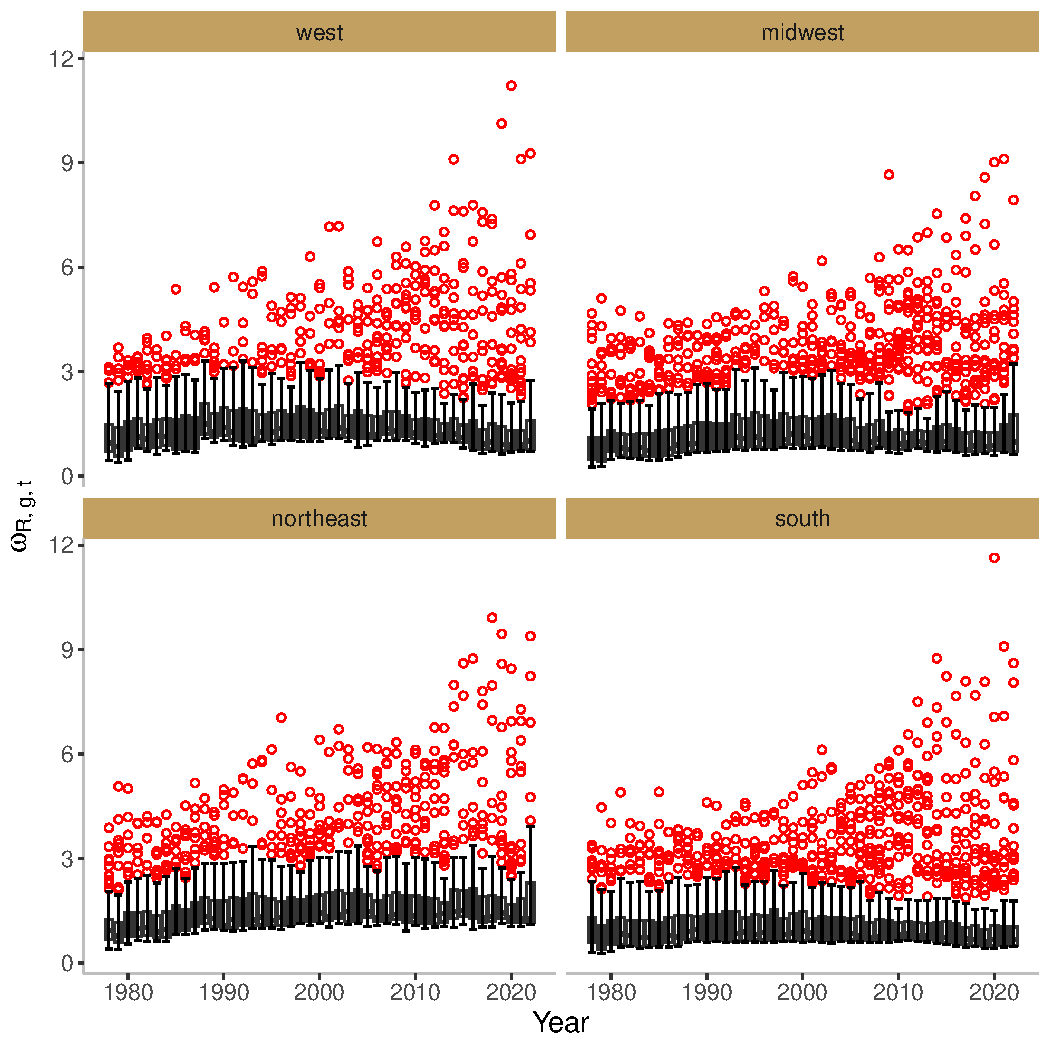
\includegraphics[width = 6in, height =5in]{figs/weightsTime.pdf}
\end{figure}




\section{Impact of one-year ahead inflation expectations}

\subsection{Preliminary results}

Figure \ref{fig:redform} previews and visualizes the empirical estimates to follow. The left panels report results using the Michigan survey shift-share, while the right is for the CPS shift-share instrument. The top panels (\ref{subfig:redform:stage1:michigan}-\ref{subfig:redform:stage1:cps}) plot the first stage, and the bottom panels (\ref{subfig:redform:stage2:michigan}-\ref{subfig:redform:stage2:cps}) visualize the reduced-form regression of regional inflation on the Bartik instrument. In each panel, the solid line is the linear regression equation. The shift-shares correlate strongly with the Michigan survey expectations. The Michigan survey-based shift-share instrument correlates more closely with expectations than the instrument calculated with CPS78 shares.  

Panels (\ref{subfig:redform:stage2:michigan}-\ref{subfig:redform:stage2:cps}) plot the results from a reduced-form panel regression of the inflation rate on the predicted inflation expectations. Regardless of the instrument, there is a strong positive relationship between predicted inflation expectations and inflation.

The rest of the analysis probes the interpretation of the results in Figure \ref{fig:redform}.

\begin{figure}
\centering
\caption{Inflation expectations and inflation: reduced-form estimates.}\label{fig:redform}
\begin{subfigure}[t]{0.475\textwidth}
\centering
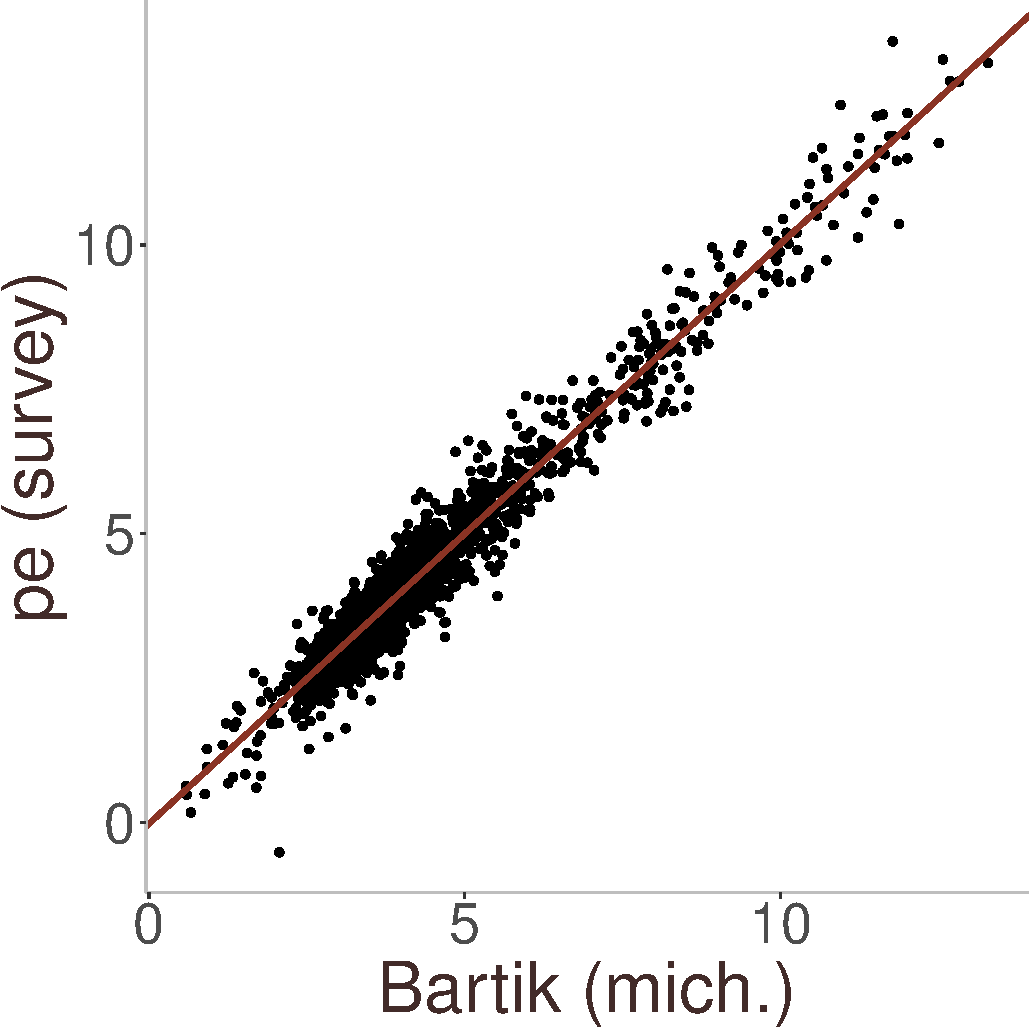
\includegraphics[width = 3in, height =3in]{figs/firststage}
\caption{First stage: shares calculated from Michigan survey.  }\label{subfig:redform:stage1:michigan}
\end{subfigure}
\quad
\begin{subfigure}[t]{0.475\textwidth}
\centering
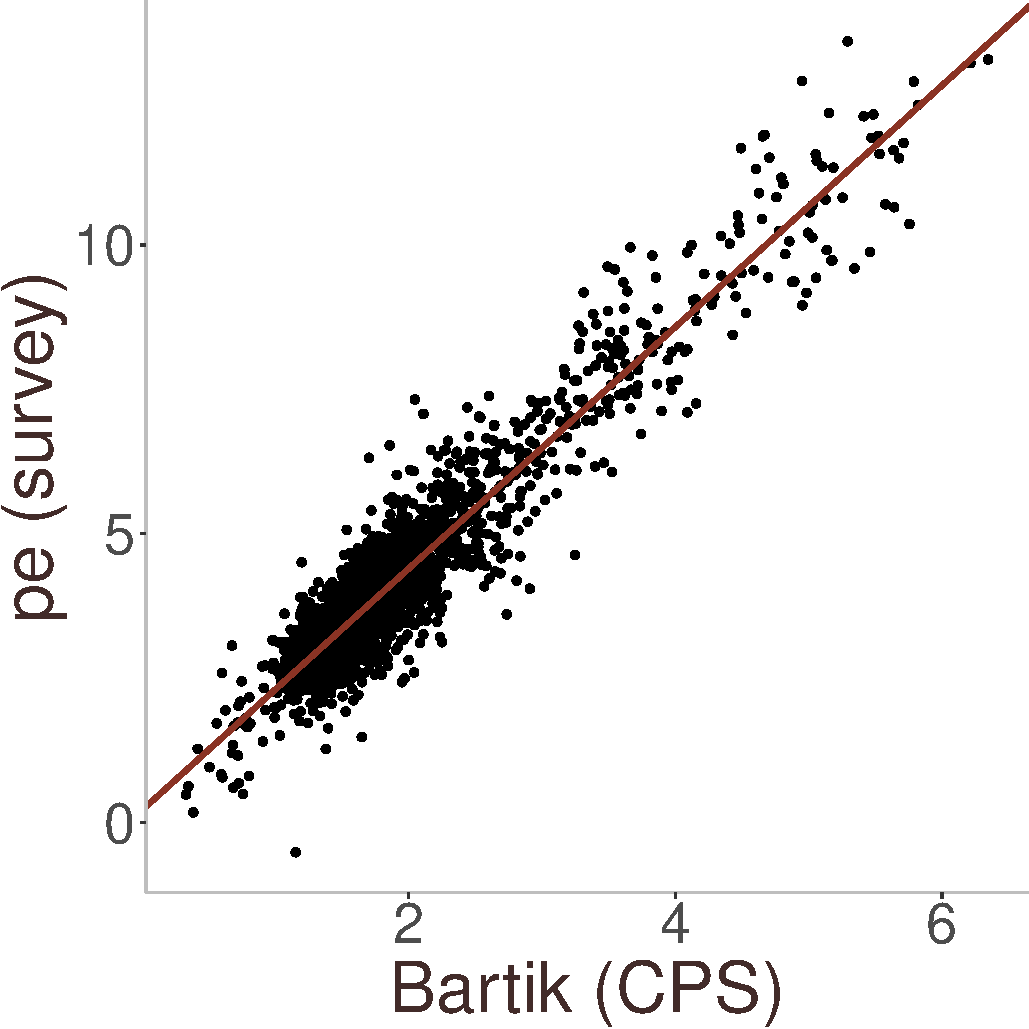
\includegraphics[width =3in, height =3in]{figs/firststage_cps}
\caption{First stage: shares calculated from 1978.1 CPS.}\label{subfig:redform:stage1:cps}
\end{subfigure}
\vfill
\begin{subfigure}[t]{0.475\textwidth}
\centering
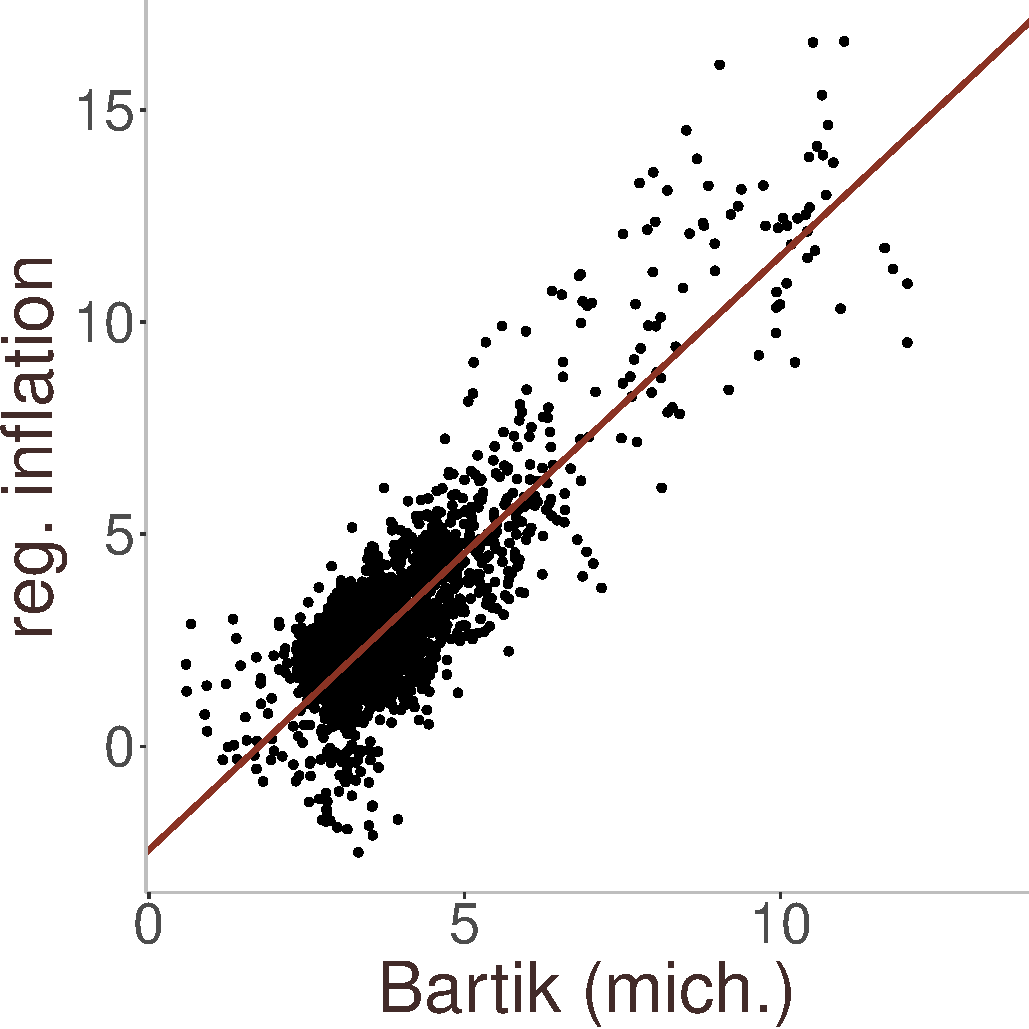
\includegraphics[width =3in, height =3in]{figs/redform}
\caption{OLS regression: Michigan shares.}\label{subfig:redform:stage2:michigan}
\end{subfigure}
\begin{subfigure}[t]{0.475\textwidth}
\centering
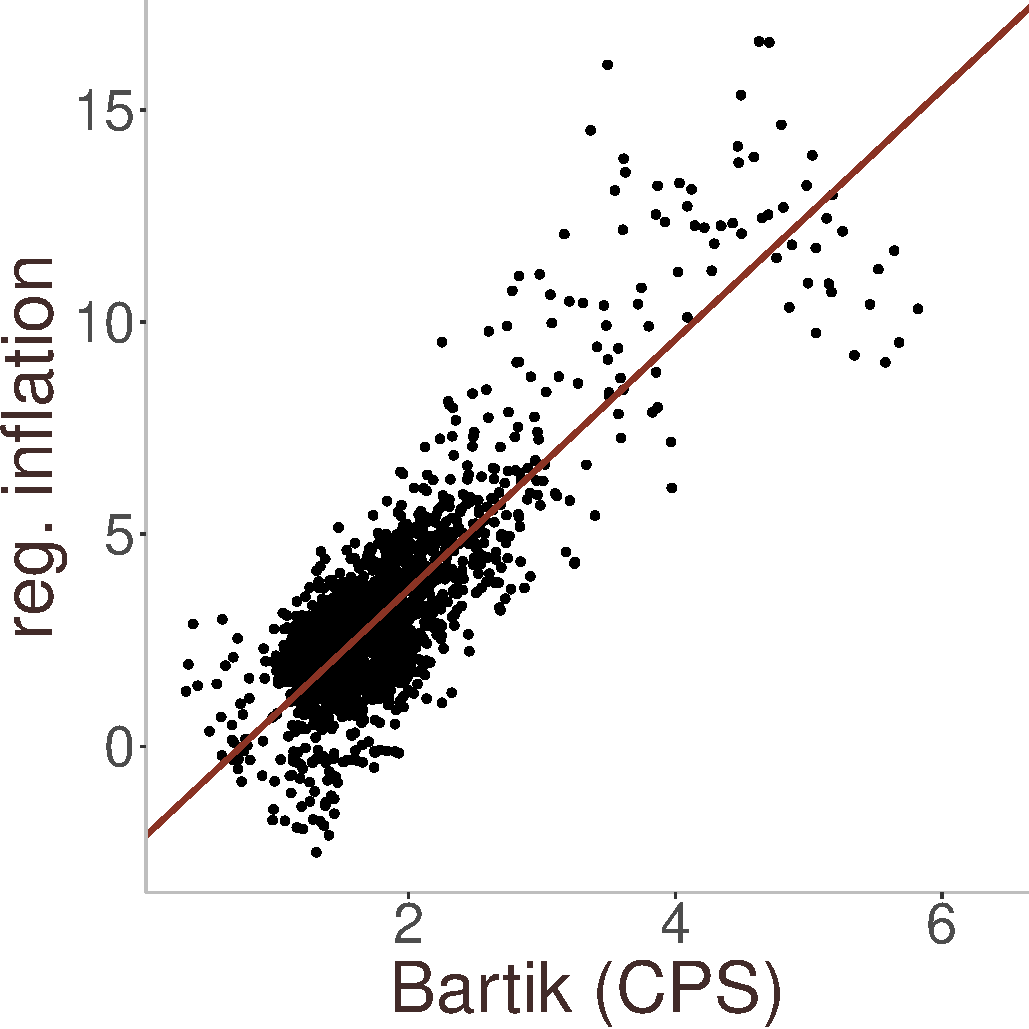
\includegraphics[width =3in, height =3in]{figs/redform_cps}
\caption{OLS regression: CPS78 shares.}\label{subfig:redform:stage2:cps}
\end{subfigure}
\end{figure}


\subsection{2sls estimates}



Tables \ref{tab:base:out:2sls:stage1}-\ref{tab:base:out:2sls:stage2} present the two-stage least squares estimates of the impact that consumer inflation expectations have on regional inflation rates. The left-hand column details the coefficient estimate with the Michigan survey measure of group shares. The right column encompasses the CPS 1978.1 population shares. In both instances, constructing the instrument uses a regional leave-one-out approach. The results presented include a set of control variables and region and time fixed effects—the latter controls for aggregate business cycle factors common to all regions. The control variables include the regional unemployment rate, four lags of inflation, expectations about future unemployment, survey measures for current and anticipated financial well-being and conditions, and regional expected gas prices.\footnote{The results are robust to instrumenting for unemployment and expected gas prices.}

\begin{table}

\caption{\label{tab:base:out:2sls:stage1}2SLS: first stage}
\centering
\begin{threeparttable}
\begin{tabular}[t]{lll}
\toprule
  & survey & CPS78\\
\midrule
\cellcolor{gray!6}{Dependent Var.:} & \cellcolor{gray!6}{pe} & \cellcolor{gray!6}{pe}\\
\addlinespace
 &  & \\
\addlinespace
\cellcolor{gray!6}{Bartik} & \cellcolor{gray!6}{0.2474*** (0.0611)} & \cellcolor{gray!6}{0.4478** (0.1448)}\\
\addlinespace
Controls & Yes & Yes\\
\addlinespace
\cellcolor{gray!6}{Fixed-Effects:} & \cellcolor{gray!6}{------------------} & \cellcolor{gray!6}{-----------------}\\
\addlinespace
REGION & Yes & Yes\\
\addlinespace
\cellcolor{gray!6}{TIME} & \cellcolor{gray!6}{Yes} & \cellcolor{gray!6}{Yes}\\
\addlinespace
\_\_\_\_\_\_\_\_\_\_\_\_\_\_\_ & \_\_\_\_\_\_\_\_\_\_\_\_\_\_\_\_\_\_ & \_\_\_\_\_\_\_\_\_\_\_\_\_\_\_\_\_\\
\addlinespace
\cellcolor{gray!6}{S.E. type} & \cellcolor{gray!6}{Drisco.-Kra. (L=4)} & \cellcolor{gray!6}{Drisc.-Kra. (L=4)}\\
\addlinespace
Observations & 1,387 & 1,387\\
\addlinespace
\cellcolor{gray!6}{R2} & \cellcolor{gray!6}{0.80353} & \cellcolor{gray!6}{0.80133}\\
\addlinespace
Within R2 & 0.13739 & 0.12774\\
\bottomrule
\end{tabular}
\begin{tablenotes}
\item \textit{Note: } 
\item First stage from 2sls panel regression of regional inflation on expected inflation. In the first stage, the Bartik instrument is a good predictor of inflation expectations. Instruments computed using a leave-one-out procedure. Survey is the shift-share instrument using Michigan survey shares. CPS78 is constructed from the 1978.1 CPS.
\item[1] Signif. codes: * = .05; ** = .01; *** = .001.
\end{tablenotes}
\end{threeparttable}
\end{table}

\begin{table}

\caption{\label{tab:base:out:2sls:stage2}2SLS: coefficient estimates}
\centering
\begin{threeparttable}
\begin{tabular}[t]{lll}
\toprule
  & survey & CPS78\\
\midrule
\cellcolor{gray!6}{Dependent Var.:} & \cellcolor{gray!6}{RegInf} & \cellcolor{gray!6}{RegInf}\\
\addlinespace
 &  & \\
\addlinespace
\cellcolor{gray!6}{pe} & \cellcolor{gray!6}{0.3351* (0.1406)} & \cellcolor{gray!6}{0.5465** (0.1939)}\\
\addlinespace
Controls & Yes & Yes\\
\addlinespace
\cellcolor{gray!6}{Fixed-Effects:} & \cellcolor{gray!6}{----------------} & \cellcolor{gray!6}{-----------------}\\
\addlinespace
REGION & Yes & Yes\\
\addlinespace
\cellcolor{gray!6}{TIME} & \cellcolor{gray!6}{Yes} & \cellcolor{gray!6}{Yes}\\
\addlinespace
\_\_\_\_\_\_\_\_\_\_\_\_\_\_\_ & \_\_\_\_\_\_\_\_\_\_\_\_\_\_\_\_ & \_\_\_\_\_\_\_\_\_\_\_\_\_\_\_\_\_\\
\addlinespace
\cellcolor{gray!6}{S.E. type} & \cellcolor{gray!6}{Dris.-Kra. (L=4)} & \cellcolor{gray!6}{Drisc.-Kra. (L=4)}\\
\addlinespace
Observations & 1,387 & 1,387\\
\addlinespace
\cellcolor{gray!6}{R2} & \cellcolor{gray!6}{0.95399} & \cellcolor{gray!6}{0.93969}\\
\addlinespace
Within R2 & 0.55429 & 0.41579\\
\bottomrule
\end{tabular}
\begin{tablenotes}
\item \textit{Note: } 
\item Coefficient estimates from 2sls panel regression of regional inflation on expected inflation. Instruments computed using a leave-one-out procedure. Survey is the shift-share instrument using Michigan survey shares. CPS78 is constructed from the 1978.1 CPS.
\item[1] Signif. codes: * = .05; ** = .01; *** = .001.
\end{tablenotes}
\end{threeparttable}
\end{table}


Table \ref{tab:base:out:2sls:stage1} provides first stage estimates. The Bartik instrument is relevant and has significant predictive power for inflation expectations. The Durbin-Wu-Hausman test statistic for endogeneity is 8.074, rejecting the consistency of OLS at a 1\% significance level. The first-stage F-statistic is 52.4, which is significant at the .1\% level. While the identifying variation in the shares is plausibly exogenous to regional inflation rates, in the case of CPS78, it is possible to probe the exogeneity assumption by examining whether those 1978 population shares are predictive of the regression covariates. In each case, there is no significant correlation between the covariates and the CPS group shares, and the regression coefficients are economically close to zero.

The second stage estimates in Table \ref{tab:base:out:2sls:stage2} identify a significant and positive effect from subjective inflation expectations to inflation rates. Using the Michigan survey shares, the estimated coefficient is $0.3275$, so a 1\% increase in the average expected inflation rate in a region would lead to a 32 basis point increase in that region's inflation rate. The estimated coefficient is significant at the 5\% level. The estimated effect is stronger using the CPS 1978.1 population shares. The estimated coefficient is $0.5464$, at a 1\% significance level. Here, the pass-through from inflation expectations to inflation is greater than $\nicefrac{1}{2}$.  

When comparing the 2sls coefficient estimates to those in Figure \ref{subfig:intro:reg}, OLS estimates, where the correlation between inflation expectations and inflation was around $0.06$, are biased downwards. The empirical model does not account for spatial spillovers. Much like the literature on regional fiscal multipliers, after accounting for cross-regional spillovers -- an increase in inflation expectations in one region also impacts the demand for goods produced in a different region -- the aggregate impact of expectations is stronger than the regional effect. In Figure \ref{subfig:intro:us} it was seen that the correlation between aggregate inflation expectations and aggregate inflation rates is $0.18$. A similar magnitude in the 2sls estimates would imply a pass-through of approximately $1.0-1.6$.  

The coefficient estimates are in line with the theoretical analysis in \cite{Werning:expectsWP}, which studies pass-through in a variety of conventional pricing models with time-dependent price rigidities while not making \emph{a priori} assumptions about the formation of subjective inflation expectations. While the pass-through from expectations to inflation can take any positive value, \cite{Werning:expectsWP} shows that for the Calvo and Taylor models of price stickiness that pass through should be in the range $\left[\nicefrac{1}{2},1\right]$, and possibly above one in a more general framework. While the regional estimates in Table \ref{tab:base:out:2sls:stage2} are on the lower end, or slightly below, of this range, after accounting for regional spillovers, the estimates are in line with the theoretical predictions.

The panel data is susceptible to a potential finite sample bias. Of particular concern are the data's ``small N/big T'' dimensions. Table \ref{tab:bias:out:2sls:stage2} applies a split-sample jackknife bias correction (\cite{FernandezValWeidner:FE}). After correcting for finite sample bias in both the cross-section and time dimensions, the estimated effect of inflation expectations increases slightly.

\begin{table}
\centering
\caption{\label{tab:bias:out:2sls:stage2}Bias Correction}
\centering
\begin{threeparttable}
\begin{tabular}[t]{lrr}
\toprule
  & survey shares & CPS78 shares\\
\midrule
\cellcolor{gray!10}{coeff.} & \cellcolor{gray!10}{0.3753} & \cellcolor{gray!10}{0.5999}\\
se & 0.1356 & 0.1940\\
\bottomrule
\end{tabular}
\begin{tablenotes}
\item \textit{Note: } 
\item Applies the split-sample jacknife bias correction to the 2sls coefficient estimates. The column ``survey shares'' computes shares from Michigan survey,``CPS78 shares'' uses the CPS 1978.1 shares.
\end{tablenotes}
\end{threeparttable}
\end{table}


Another way to measure the impact of expectations is by estimating an impulse response function. The empirical model is not a vector autoregression, but a local projections approach can estimate the impulse response function.\footnote{See \cite{Jorda:LP}.}. The impulse response function comes from running 2sls regressions of the form
$$ E_t\pi^R_{t+h} = \delta_{R,h} + \beta_h\pi^e_{R,t} + \gamma'_h x_{R,h} + \mu_{t,h} + \varepsilon_{R,h,t}$$
for horizons $h=1,...,H$. The impulse response function then is given by $\left(\beta_h\right)_{1\leq h\leq H}$. The estimates are provided in Figure \ref{fig:base:irf}.

On impact, inflation expectations have a significant positive effect on inflation. There is a cyclical dampening process that is mean-reverting within 12 months. However, the confidence bands are wide in future quarters and cannot rule out any lingering impacts. Thus, the estimates suggest a moderate contemporaneous response to inflation from a shock to inflation expectations. The lack of a strongly persistent expectation effect could reflect the specific U.S. inflation history. It would be interesting to extend the analysis to countries with persistently, or volatile, inflation.


\begin{figure}
\centering
\caption{Impulse responses}\label{fig:base:irf}
\begin{subfigure}[t]{0.475\textwidth}
\centering
% Created by tikzDevice version 0.12.3.1 on 2023-11-03 11:03:16
% !TEX encoding = UTF-8 Unicode
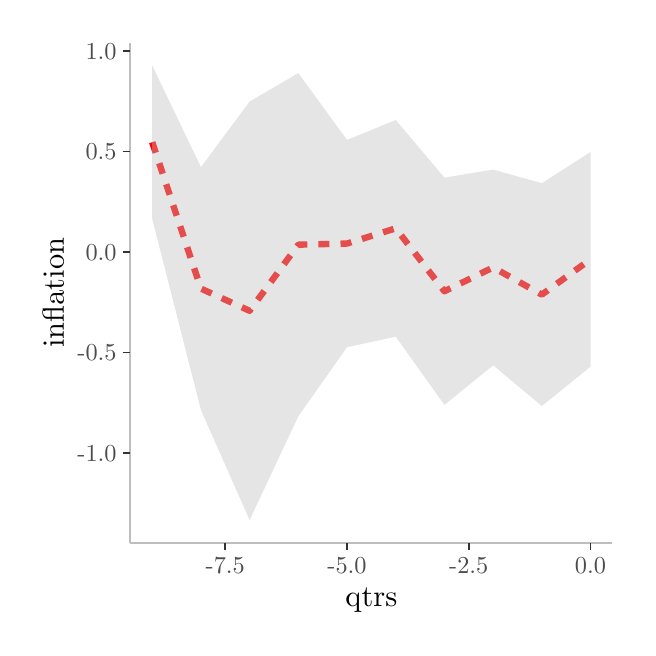
\begin{tikzpicture}[x=1pt,y=1pt]
\definecolor{fillColor}{RGB}{255,255,255}
\path[use as bounding box,fill=fillColor,fill opacity=0.00] (0,0) rectangle (216.81,216.81);
\begin{scope}
\path[clip] (  0.00,  0.00) rectangle (216.81,216.81);
\definecolor{drawColor}{RGB}{255,255,255}
\definecolor{fillColor}{RGB}{255,255,255}

\path[draw=drawColor,line width= 0.6pt,line join=round,line cap=round,fill=fillColor] (  0.00,  0.00) rectangle (216.81,216.81);
\end{scope}
\begin{scope}
\path[clip] ( 37.09, 30.69) rectangle (211.31,211.31);
\definecolor{drawColor}{RGB}{255,255,255}

\path[draw=drawColor,line width= 0.6pt,line join=round] ( 37.09, 63.17) --
	(211.31, 63.17);

\path[draw=drawColor,line width= 0.6pt,line join=round] ( 37.09, 99.46) --
	(211.31, 99.46);

\path[draw=drawColor,line width= 0.6pt,line join=round] ( 37.09,135.75) --
	(211.31,135.75);

\path[draw=drawColor,line width= 0.6pt,line join=round] ( 37.09,172.05) --
	(211.31,172.05);

\path[draw=drawColor,line width= 0.6pt,line join=round] ( 37.09,208.34) --
	(211.31,208.34);

\path[draw=drawColor,line width= 0.6pt,line join=round] ( 71.41, 30.69) --
	( 71.41,211.31);

\path[draw=drawColor,line width= 0.6pt,line join=round] (115.40, 30.69) --
	(115.40,211.31);

\path[draw=drawColor,line width= 0.6pt,line join=round] (159.40, 30.69) --
	(159.40,211.31);

\path[draw=drawColor,line width= 0.6pt,line join=round] (203.39, 30.69) --
	(203.39,211.31);
\definecolor{drawColor}{RGB}{255,0,0}

\path[draw=drawColor,line width= 2.3pt,dash pattern=on 4pt off 4pt ,line join=round] ( 45.01,175.42) --
	( 62.61,122.52) --
	( 80.20,114.50) --
	( 97.80,138.39) --
	(115.40,138.80) --
	(133.00,144.30) --
	(150.60,121.56) --
	(168.19,130.17) --
	(185.79,120.35) --
	(203.39,133.10);
\definecolor{fillColor}{RGB}{190,190,190}

\path[fill=fillColor,fill opacity=0.40] ( 45.01,203.10) --
	( 62.61,166.39) --
	( 80.20,190.11) --
	( 97.80,200.37) --
	(115.40,176.23) --
	(133.00,183.45) --
	(150.60,162.60) --
	(168.19,165.52) --
	(185.79,160.60) --
	(203.39,171.87) --
	(203.39, 94.33) --
	(185.79, 80.10) --
	(168.19, 94.83) --
	(150.60, 80.51) --
	(133.00,105.15) --
	(115.40,101.36) --
	( 97.80, 76.41) --
	( 80.20, 38.90) --
	( 62.61, 78.65) --
	( 45.01,147.74) --
	cycle;

\path[] ( 45.01,203.10) --
	( 62.61,166.39) --
	( 80.20,190.11) --
	( 97.80,200.37) --
	(115.40,176.23) --
	(133.00,183.45) --
	(150.60,162.60) --
	(168.19,165.52) --
	(185.79,160.60) --
	(203.39,171.87);

\path[] (203.39, 94.33) --
	(185.79, 80.10) --
	(168.19, 94.83) --
	(150.60, 80.51) --
	(133.00,105.15) --
	(115.40,101.36) --
	( 97.80, 76.41) --
	( 80.20, 38.90) --
	( 62.61, 78.65) --
	( 45.01,147.74);
\end{scope}
\begin{scope}
\path[clip] (  0.00,  0.00) rectangle (216.81,216.81);
\definecolor{drawColor}{RGB}{190,190,190}

\path[draw=drawColor,line width= 0.6pt,line join=round] ( 37.09, 30.69) --
	( 37.09,211.31);
\end{scope}
\begin{scope}
\path[clip] (  0.00,  0.00) rectangle (216.81,216.81);
\definecolor{drawColor}{gray}{0.30}

\node[text=drawColor,anchor=base east,inner sep=0pt, outer sep=0pt, scale=  0.88] at ( 32.14, 60.13) {-1.0};

\node[text=drawColor,anchor=base east,inner sep=0pt, outer sep=0pt, scale=  0.88] at ( 32.14, 96.43) {-0.5};

\node[text=drawColor,anchor=base east,inner sep=0pt, outer sep=0pt, scale=  0.88] at ( 32.14,132.72) {0.0};

\node[text=drawColor,anchor=base east,inner sep=0pt, outer sep=0pt, scale=  0.88] at ( 32.14,169.02) {0.5};

\node[text=drawColor,anchor=base east,inner sep=0pt, outer sep=0pt, scale=  0.88] at ( 32.14,205.31) {1.0};
\end{scope}
\begin{scope}
\path[clip] (  0.00,  0.00) rectangle (216.81,216.81);
\definecolor{drawColor}{gray}{0.20}

\path[draw=drawColor,line width= 0.6pt,line join=round] ( 34.34, 63.17) --
	( 37.09, 63.17);

\path[draw=drawColor,line width= 0.6pt,line join=round] ( 34.34, 99.46) --
	( 37.09, 99.46);

\path[draw=drawColor,line width= 0.6pt,line join=round] ( 34.34,135.75) --
	( 37.09,135.75);

\path[draw=drawColor,line width= 0.6pt,line join=round] ( 34.34,172.05) --
	( 37.09,172.05);

\path[draw=drawColor,line width= 0.6pt,line join=round] ( 34.34,208.34) --
	( 37.09,208.34);
\end{scope}
\begin{scope}
\path[clip] (  0.00,  0.00) rectangle (216.81,216.81);
\definecolor{drawColor}{RGB}{190,190,190}

\path[draw=drawColor,line width= 0.6pt,line join=round] ( 37.09, 30.69) --
	(211.31, 30.69);
\end{scope}
\begin{scope}
\path[clip] (  0.00,  0.00) rectangle (216.81,216.81);
\definecolor{drawColor}{gray}{0.20}

\path[draw=drawColor,line width= 0.6pt,line join=round] ( 71.41, 27.94) --
	( 71.41, 30.69);

\path[draw=drawColor,line width= 0.6pt,line join=round] (115.40, 27.94) --
	(115.40, 30.69);

\path[draw=drawColor,line width= 0.6pt,line join=round] (159.40, 27.94) --
	(159.40, 30.69);

\path[draw=drawColor,line width= 0.6pt,line join=round] (203.39, 27.94) --
	(203.39, 30.69);
\end{scope}
\begin{scope}
\path[clip] (  0.00,  0.00) rectangle (216.81,216.81);
\definecolor{drawColor}{gray}{0.30}

\node[text=drawColor,anchor=base,inner sep=0pt, outer sep=0pt, scale=  0.88] at ( 71.41, 19.68) {-7.5};

\node[text=drawColor,anchor=base,inner sep=0pt, outer sep=0pt, scale=  0.88] at (115.40, 19.68) {-5.0};

\node[text=drawColor,anchor=base,inner sep=0pt, outer sep=0pt, scale=  0.88] at (159.40, 19.68) {-2.5};

\node[text=drawColor,anchor=base,inner sep=0pt, outer sep=0pt, scale=  0.88] at (203.39, 19.68) {0.0};
\end{scope}
\begin{scope}
\path[clip] (  0.00,  0.00) rectangle (216.81,216.81);
\definecolor{drawColor}{RGB}{0,0,0}

\node[text=drawColor,anchor=base,inner sep=0pt, outer sep=0pt, scale=  1.10] at (124.20,  7.64) {qtrs};
\end{scope}
\begin{scope}
\path[clip] (  0.00,  0.00) rectangle (216.81,216.81);
\definecolor{drawColor}{RGB}{0,0,0}

\node[text=drawColor,rotate= 90.00,anchor=base,inner sep=0pt, outer sep=0pt, scale=  1.10] at ( 13.08,121.00) {inflation};
\end{scope}
\end{tikzpicture}

\caption{cps shares}
\end{subfigure}
\quad
\begin{subfigure}[t]{0.475\textwidth}
\centering
% Created by tikzDevice version 0.12.3.1 on 2023-10-19 11:54:22
% !TEX encoding = UTF-8 Unicode
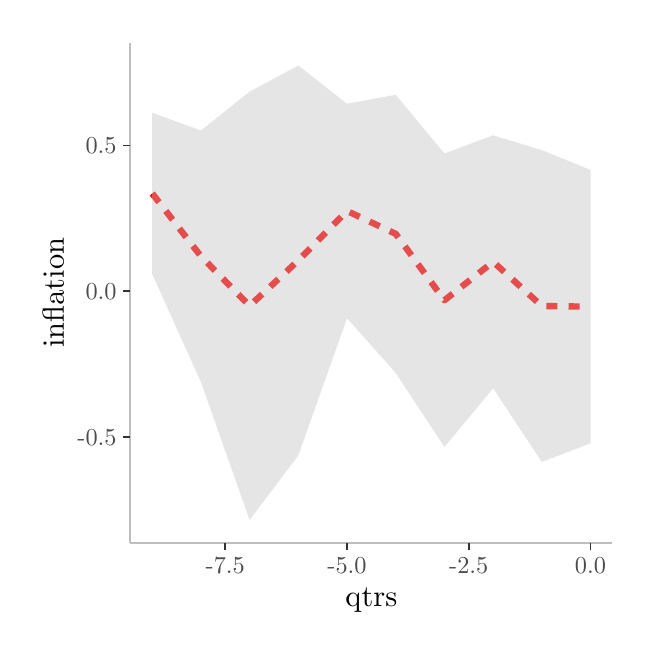
\begin{tikzpicture}[x=1pt,y=1pt]
\definecolor{fillColor}{RGB}{255,255,255}
\path[use as bounding box,fill=fillColor,fill opacity=0.00] (0,0) rectangle (216.81,216.81);
\begin{scope}
\path[clip] (  0.00,  0.00) rectangle (216.81,216.81);
\definecolor{drawColor}{RGB}{255,255,255}
\definecolor{fillColor}{RGB}{255,255,255}

\path[draw=drawColor,line width= 0.6pt,line join=round,line cap=round,fill=fillColor] (  0.00,  0.00) rectangle (216.81,216.81);
\end{scope}
\begin{scope}
\path[clip] ( 37.09, 30.69) rectangle (211.31,211.31);
\definecolor{drawColor}{RGB}{255,255,255}

\path[draw=drawColor,line width= 0.6pt,line join=round] ( 37.09, 68.88) --
	(211.31, 68.88);

\path[draw=drawColor,line width= 0.6pt,line join=round] ( 37.09,121.58) --
	(211.31,121.58);

\path[draw=drawColor,line width= 0.6pt,line join=round] ( 37.09,174.28) --
	(211.31,174.28);

\path[draw=drawColor,line width= 0.6pt,line join=round] ( 71.41, 30.69) --
	( 71.41,211.31);

\path[draw=drawColor,line width= 0.6pt,line join=round] (115.40, 30.69) --
	(115.40,211.31);

\path[draw=drawColor,line width= 0.6pt,line join=round] (159.40, 30.69) --
	(159.40,211.31);

\path[draw=drawColor,line width= 0.6pt,line join=round] (203.39, 30.69) --
	(203.39,211.31);
\definecolor{drawColor}{RGB}{255,0,0}

\path[draw=drawColor,line width= 2.3pt,dash pattern=on 4pt off 4pt ,line join=round] ( 45.01,156.90) --
	( 62.61,134.20) --
	( 80.20,116.30) --
	( 97.80,132.68) --
	(115.40,150.58) --
	(133.00,142.31) --
	(150.60,118.31) --
	(168.19,132.20) --
	(185.79,116.23) --
	(203.39,116.00);
\definecolor{fillColor}{RGB}{190,190,190}

\path[fill=fillColor,fill opacity=0.40] ( 45.01,186.05) --
	( 62.61,179.64) --
	( 80.20,193.70) --
	( 97.80,203.10) --
	(115.40,189.31) --
	(133.00,192.56) --
	(150.60,171.34) --
	(168.19,177.89) --
	(185.79,172.57) --
	(203.39,165.39) --
	(203.39, 66.62) --
	(185.79, 59.89) --
	(168.19, 86.51) --
	(150.60, 65.29) --
	(133.00, 92.06) --
	(115.40,111.84) --
	( 97.80, 62.27) --
	( 80.20, 38.90) --
	( 62.61, 88.76) --
	( 45.01,127.74) --
	cycle;

\path[] ( 45.01,186.05) --
	( 62.61,179.64) --
	( 80.20,193.70) --
	( 97.80,203.10) --
	(115.40,189.31) --
	(133.00,192.56) --
	(150.60,171.34) --
	(168.19,177.89) --
	(185.79,172.57) --
	(203.39,165.39);

\path[] (203.39, 66.62) --
	(185.79, 59.89) --
	(168.19, 86.51) --
	(150.60, 65.29) --
	(133.00, 92.06) --
	(115.40,111.84) --
	( 97.80, 62.27) --
	( 80.20, 38.90) --
	( 62.61, 88.76) --
	( 45.01,127.74);
\end{scope}
\begin{scope}
\path[clip] (  0.00,  0.00) rectangle (216.81,216.81);
\definecolor{drawColor}{RGB}{190,190,190}

\path[draw=drawColor,line width= 0.6pt,line join=round] ( 37.09, 30.69) --
	( 37.09,211.31);
\end{scope}
\begin{scope}
\path[clip] (  0.00,  0.00) rectangle (216.81,216.81);
\definecolor{drawColor}{gray}{0.30}

\node[text=drawColor,anchor=base east,inner sep=0pt, outer sep=0pt, scale=  0.88] at ( 32.14, 65.85) {-0.5};

\node[text=drawColor,anchor=base east,inner sep=0pt, outer sep=0pt, scale=  0.88] at ( 32.14,118.55) {0.0};

\node[text=drawColor,anchor=base east,inner sep=0pt, outer sep=0pt, scale=  0.88] at ( 32.14,171.25) {0.5};
\end{scope}
\begin{scope}
\path[clip] (  0.00,  0.00) rectangle (216.81,216.81);
\definecolor{drawColor}{gray}{0.20}

\path[draw=drawColor,line width= 0.6pt,line join=round] ( 34.34, 68.88) --
	( 37.09, 68.88);

\path[draw=drawColor,line width= 0.6pt,line join=round] ( 34.34,121.58) --
	( 37.09,121.58);

\path[draw=drawColor,line width= 0.6pt,line join=round] ( 34.34,174.28) --
	( 37.09,174.28);
\end{scope}
\begin{scope}
\path[clip] (  0.00,  0.00) rectangle (216.81,216.81);
\definecolor{drawColor}{RGB}{190,190,190}

\path[draw=drawColor,line width= 0.6pt,line join=round] ( 37.09, 30.69) --
	(211.31, 30.69);
\end{scope}
\begin{scope}
\path[clip] (  0.00,  0.00) rectangle (216.81,216.81);
\definecolor{drawColor}{gray}{0.20}

\path[draw=drawColor,line width= 0.6pt,line join=round] ( 71.41, 27.94) --
	( 71.41, 30.69);

\path[draw=drawColor,line width= 0.6pt,line join=round] (115.40, 27.94) --
	(115.40, 30.69);

\path[draw=drawColor,line width= 0.6pt,line join=round] (159.40, 27.94) --
	(159.40, 30.69);

\path[draw=drawColor,line width= 0.6pt,line join=round] (203.39, 27.94) --
	(203.39, 30.69);
\end{scope}
\begin{scope}
\path[clip] (  0.00,  0.00) rectangle (216.81,216.81);
\definecolor{drawColor}{gray}{0.30}

\node[text=drawColor,anchor=base,inner sep=0pt, outer sep=0pt, scale=  0.88] at ( 71.41, 19.68) {-7.5};

\node[text=drawColor,anchor=base,inner sep=0pt, outer sep=0pt, scale=  0.88] at (115.40, 19.68) {-5.0};

\node[text=drawColor,anchor=base,inner sep=0pt, outer sep=0pt, scale=  0.88] at (159.40, 19.68) {-2.5};

\node[text=drawColor,anchor=base,inner sep=0pt, outer sep=0pt, scale=  0.88] at (203.39, 19.68) {0.0};
\end{scope}
\begin{scope}
\path[clip] (  0.00,  0.00) rectangle (216.81,216.81);
\definecolor{drawColor}{RGB}{0,0,0}

\node[text=drawColor,anchor=base,inner sep=0pt, outer sep=0pt, scale=  1.10] at (124.20,  7.64) {qtrs};
\end{scope}
\begin{scope}
\path[clip] (  0.00,  0.00) rectangle (216.81,216.81);
\definecolor{drawColor}{RGB}{0,0,0}

\node[text=drawColor,rotate= 90.00,anchor=base,inner sep=0pt, outer sep=0pt, scale=  1.10] at ( 13.08,121.00) {inflation};
\end{scope}
\end{tikzpicture}

\caption{michigan shares}
\end{subfigure}
\end{figure}

\subsection{Identification and interpretation}

The identifying assumption is that a group's subjective inflation expectations are a weighted average of the expected sector-specific inflation rates, with the weights reflecting in part that groups have heterogeneous consumption baskets. Equation (\ref{LOM}) suggests the presence of heterogeneous treatment effects from group-specific inflation expectations. The empirical procedure exploits the heterogeneity in group inflation expectations and plausibly exogenous variation in group shares to instrument for regional inflation expectations. While there are 160 different groups, their group shares can vary across regions and time, so economically, some groups may be more important than others. The interpretation of the identifying variation compares regional inflation and expectations in regions with differing degrees of exposure to these critical groups. This section explores these observations.

\cite{Pinkhametal:AER2020} exploits that the Bartik instrument estimate is a weighted average of many just identified instruments. They exploit that fact to calculate the estimation weights (``Rotemberg weights'') to understand better the variation driving identification. The analysis here applies the approach developed in \cite{Pinkhametal:AER2020}. The Rotemberg weights arise from the decomposition
$$ \beta = \sum_g \alpha_g\beta_g$$
where $\beta_g$ is the just identified estimate for group $g$. The weight $\alpha_g$ is the sensitivity of the overall estimate $\beta$ to bias emanating from misspecification in a group $g$. That is, the $\alpha_g$'s give us a measure of which groups are most driving identification and, formally, which groups to probe for endogeneity in the instrument.  

\begin{table}

\caption{\label{tab:rotweights:cps}Top-10 weighted groups: CPS shares}
\centering
\begin{threeparttable}
\begin{tabular}[t]{lrr}
\toprule
group & $\alpha_g$ & $\beta_g$\\
\midrule
\cellcolor{gray!6}{Ml,35-49,c,M,K} & \cellcolor{gray!6}{0.0151} & \cellcolor{gray!6}{1.3824}\\
\addlinespace
Ml,25-34,c,M,K & 0.0141 & 1.5614\\
\addlinespace
\cellcolor{gray!6}{Fl,35-49,c,M,K} & \cellcolor{gray!6}{0.0124} & \cellcolor{gray!6}{1.5935}\\
\addlinespace
F,25-34,c,S,NK & 0.0120 & 1.5397\\
\addlinespace
\cellcolor{gray!6}{Ml,25-34,hs,M,K} & \cellcolor{gray!6}{0.0120} & \cellcolor{gray!6}{1.5080}\\
\addlinespace
Fl,25-34,hs,M,K & 0.0117 & 1.3970\\
\addlinespace
\cellcolor{gray!6}{Ml,25-34,hs,M,NK} & \cellcolor{gray!6}{0.0110} & \cellcolor{gray!6}{1.5619}\\
\addlinespace
Fl,25-34,<hs,M,K & 0.0106 & 1.7735\\
\addlinespace
\cellcolor{gray!6}{Ml,25-34,c,S,NK} & \cellcolor{gray!6}{0.0101} & \cellcolor{gray!6}{1.4090}\\
\addlinespace
Ml,35-49,c,S,NK & 0.0101 & 1.4652\\
\bottomrule
\end{tabular}
\begin{tablenotes}
\item \textit{Note: } 
\item Group labels ordered: sex, age, educ., marital, children. Top-10 weighted groups according to the ``Rotemberg'' weights as in Bartik paper.
\end{tablenotes}
\end{threeparttable}
\end{table}

\begin{table}
\centering
\caption{\label{tab:rotweights:michigan}Top 10 weighted groups: Michigan shares}
\centering
\begin{threeparttable}
\begin{tabular}[t]{lrr}
\toprule
group id & $\alpha_g$ & $\beta_g$\\
\midrule
\cellcolor{gray!10}{Ml,18-24,h.s.,M,NK} & \cellcolor{gray!10}{0.0330} & \cellcolor{gray!10}{1.5574}\\
\addlinespace
Ml,25-34,h.s.,M,NK & 0.0177 & 1.7646\\
\addlinespace
\cellcolor{gray!10}{Ml,18-24,c+,M,NK} & \cellcolor{gray!10}{0.0174} & \cellcolor{gray!10}{1.5920}\\
\addlinespace
Fl,18-24,s.h.s.,M,NK & 0.0160 & 1.4804\\
\addlinespace
\cellcolor{gray!10}{Ml,18-24,s.c.,M,NK} & \cellcolor{gray!10}{0.0155} & \cellcolor{gray!10}{1.4664}\\
\addlinespace
Ml,18-24,h.s.,M,K & 0.0149 & 1.6477\\
\addlinespace
\cellcolor{gray!10}{Fl,18-24,h.s.,M,NK} & \cellcolor{gray!10}{0.0146} & \cellcolor{gray!10}{1.6288}\\
\addlinespace
Fl,18-24,s.c.,M,K & 0.0146 & 1.6878\\
\addlinespace
\cellcolor{gray!10}{Ml,35-49,s.c.,M,NK} & \cellcolor{gray!10}{0.0146} & \cellcolor{gray!10}{1.4254}\\
\addlinespace
Fl,25-34,h.s.,M,NK & 0.0141 & 1.8965\\
\bottomrule
\end{tabular}
\begin{tablenotes}
\item \textit{Note: } 
\item Group labels ordered: sex, age, educ., marital, children. Top-10 weighted groups according to the ``Rotemberg'' weights as in Goldsmith-Pinkham, et al (2020).
\end{tablenotes}
\end{threeparttable}
\end{table}


Tables \ref{tab:rotweights:cps}-\ref{tab:rotweights:michigan} detail the 10 groups with the highest Rotemberg weights, $\alpha_g$. Table \ref{tab:rotweights:cps} is for the case where the instrument is the CPS shares, and Table \ref{tab:rotweights:michigan} uses the Michigan survey shares. The table also lists the just-identified estimate for each of these top-10 groups. In both cases, the highest weighted groups are mostly younger with high school or above education. In the case of the CPS estimates, the highest weighted groups are 25-49 years old, and 6 of the groups have college degrees. Seven of the groups have been married with children. Using the Michigan shares instrument, Table \ref{tab:rotweights:michigan} shows that the top-10 groups are even younger than identified by the CPS instrument. Most groups are 18-24, with one 25-34 and one 35-49. These groups also have at least a high school degree, though using the Michigan survey shares, 5/10 of the top groups have a high school degree, 3 have some college, and 2 have college degrees or more. Almost all of these groups are married without children.

If the estimates in Table \ref{tab:base:out:2sls:stage2} capture heterogeneous treatment effects across groups, then it is not surprising that the two different Bartik instruments estimate different treatment effects. The Michigan shares instrument can capture shifting demographic trends in the U.S., whereas the CPS share instrument exploited differential exposure to population shares in 1978. In both cases, the group-specific effect $\beta_g$ is positive and significantly above 1 for these heavily weighted groups.  

Table \ref{tab:rotweights:groups} looks at the group weights for broader demographic groups. Reported is the sum of the $\alpha_g$'s for broader groups classified by just one demographic characteristic, e.g., sex, age, or education. Regardless of the instrument, men are weighted slightly above women, and groups above 50 receive a small share of the weights. In the CPS share instrument, as seen in Table \ref{tab:rotweights:cps}, the 25-34 age group is most heavily weighted, followed by 35-49, then 18-24. In the Michigan survey, the Rotemberg weights are declining monotonically with age. The CPS share instrument weights those with a college degree more heavily, while the Michigan survey is roughly equally sensitive to those with a high school or college degree.

Figures \ref{fig:rotweights:group}-\ref{fig:rotweights:time} provide a graphical interpretation of these heterogeneous effects. Figure \ref{fig:rotweights:group} plots the $\beta_g$ against the corresponding first stage F-statistic $F_g$. The circles denote estimates with positive $\alpha_g$, and the triangles are the negative weights. The size of the points reflects the Rotemberg weight. So, the large circles correspond to the top-10 groups in Table \ref{tab:rotweights:michigan}. Finally, the dashed line is the estimated average treatment effect. Notice that there are few negatively weighted groups, so it is natural to interpret the estimate as capturing a heterogeneous treatment effect. Second, the most heavily weighted estimates reflect groups with significant pass-through but still lie relatively close to the average effect.  

Meanwhile, Figure \ref{fig:rotweights:time} plots the Rotemberg weight for each month in the sample. Rather than summing Rotemberg weights across groups, one can also calculate which particular periods provide most of the identifying variation. Given U.S. macroeconomic history, the estimation weights in Figure \ref{fig:rotweights:time} align with what we expect. The highest weighted periods are at the end of the 1970's Great Inflation and the subsequent Volcker disinflation. The other heavily weighted periods are the Great Recession (2007-2009) and the post-pandemic accelerating inflation. These weights are sensible and help give confidence in the overall empirical strategy.

From these findings, it is reasonable to conclude that the estimated impact of expectations on inflation reflects a weighted average of heterogeneous groups. Those groups that receive the most weight tend to be younger, married, and with at least a high school degree. The identifying variation is also driven strongly by volatile periods, suggesting non-linearities in mapping inflation expectations to outcomes. By seeking exogenous variation in inflation expectations, the approach here is silent on the self-referentiality of inflation, the impact of expectations on inflation, and then inflation on expectations. However, the time-varying estimation weights seem consistent with non-linear models of endogenously heterogeneous expectations as in \cite{BranchEJ2004}, \cite{BrockHommesEconometrica1997}.



%\begin{figure}
%\centering
%\caption{Estimation weights across groups: heterogeneous effects.}
%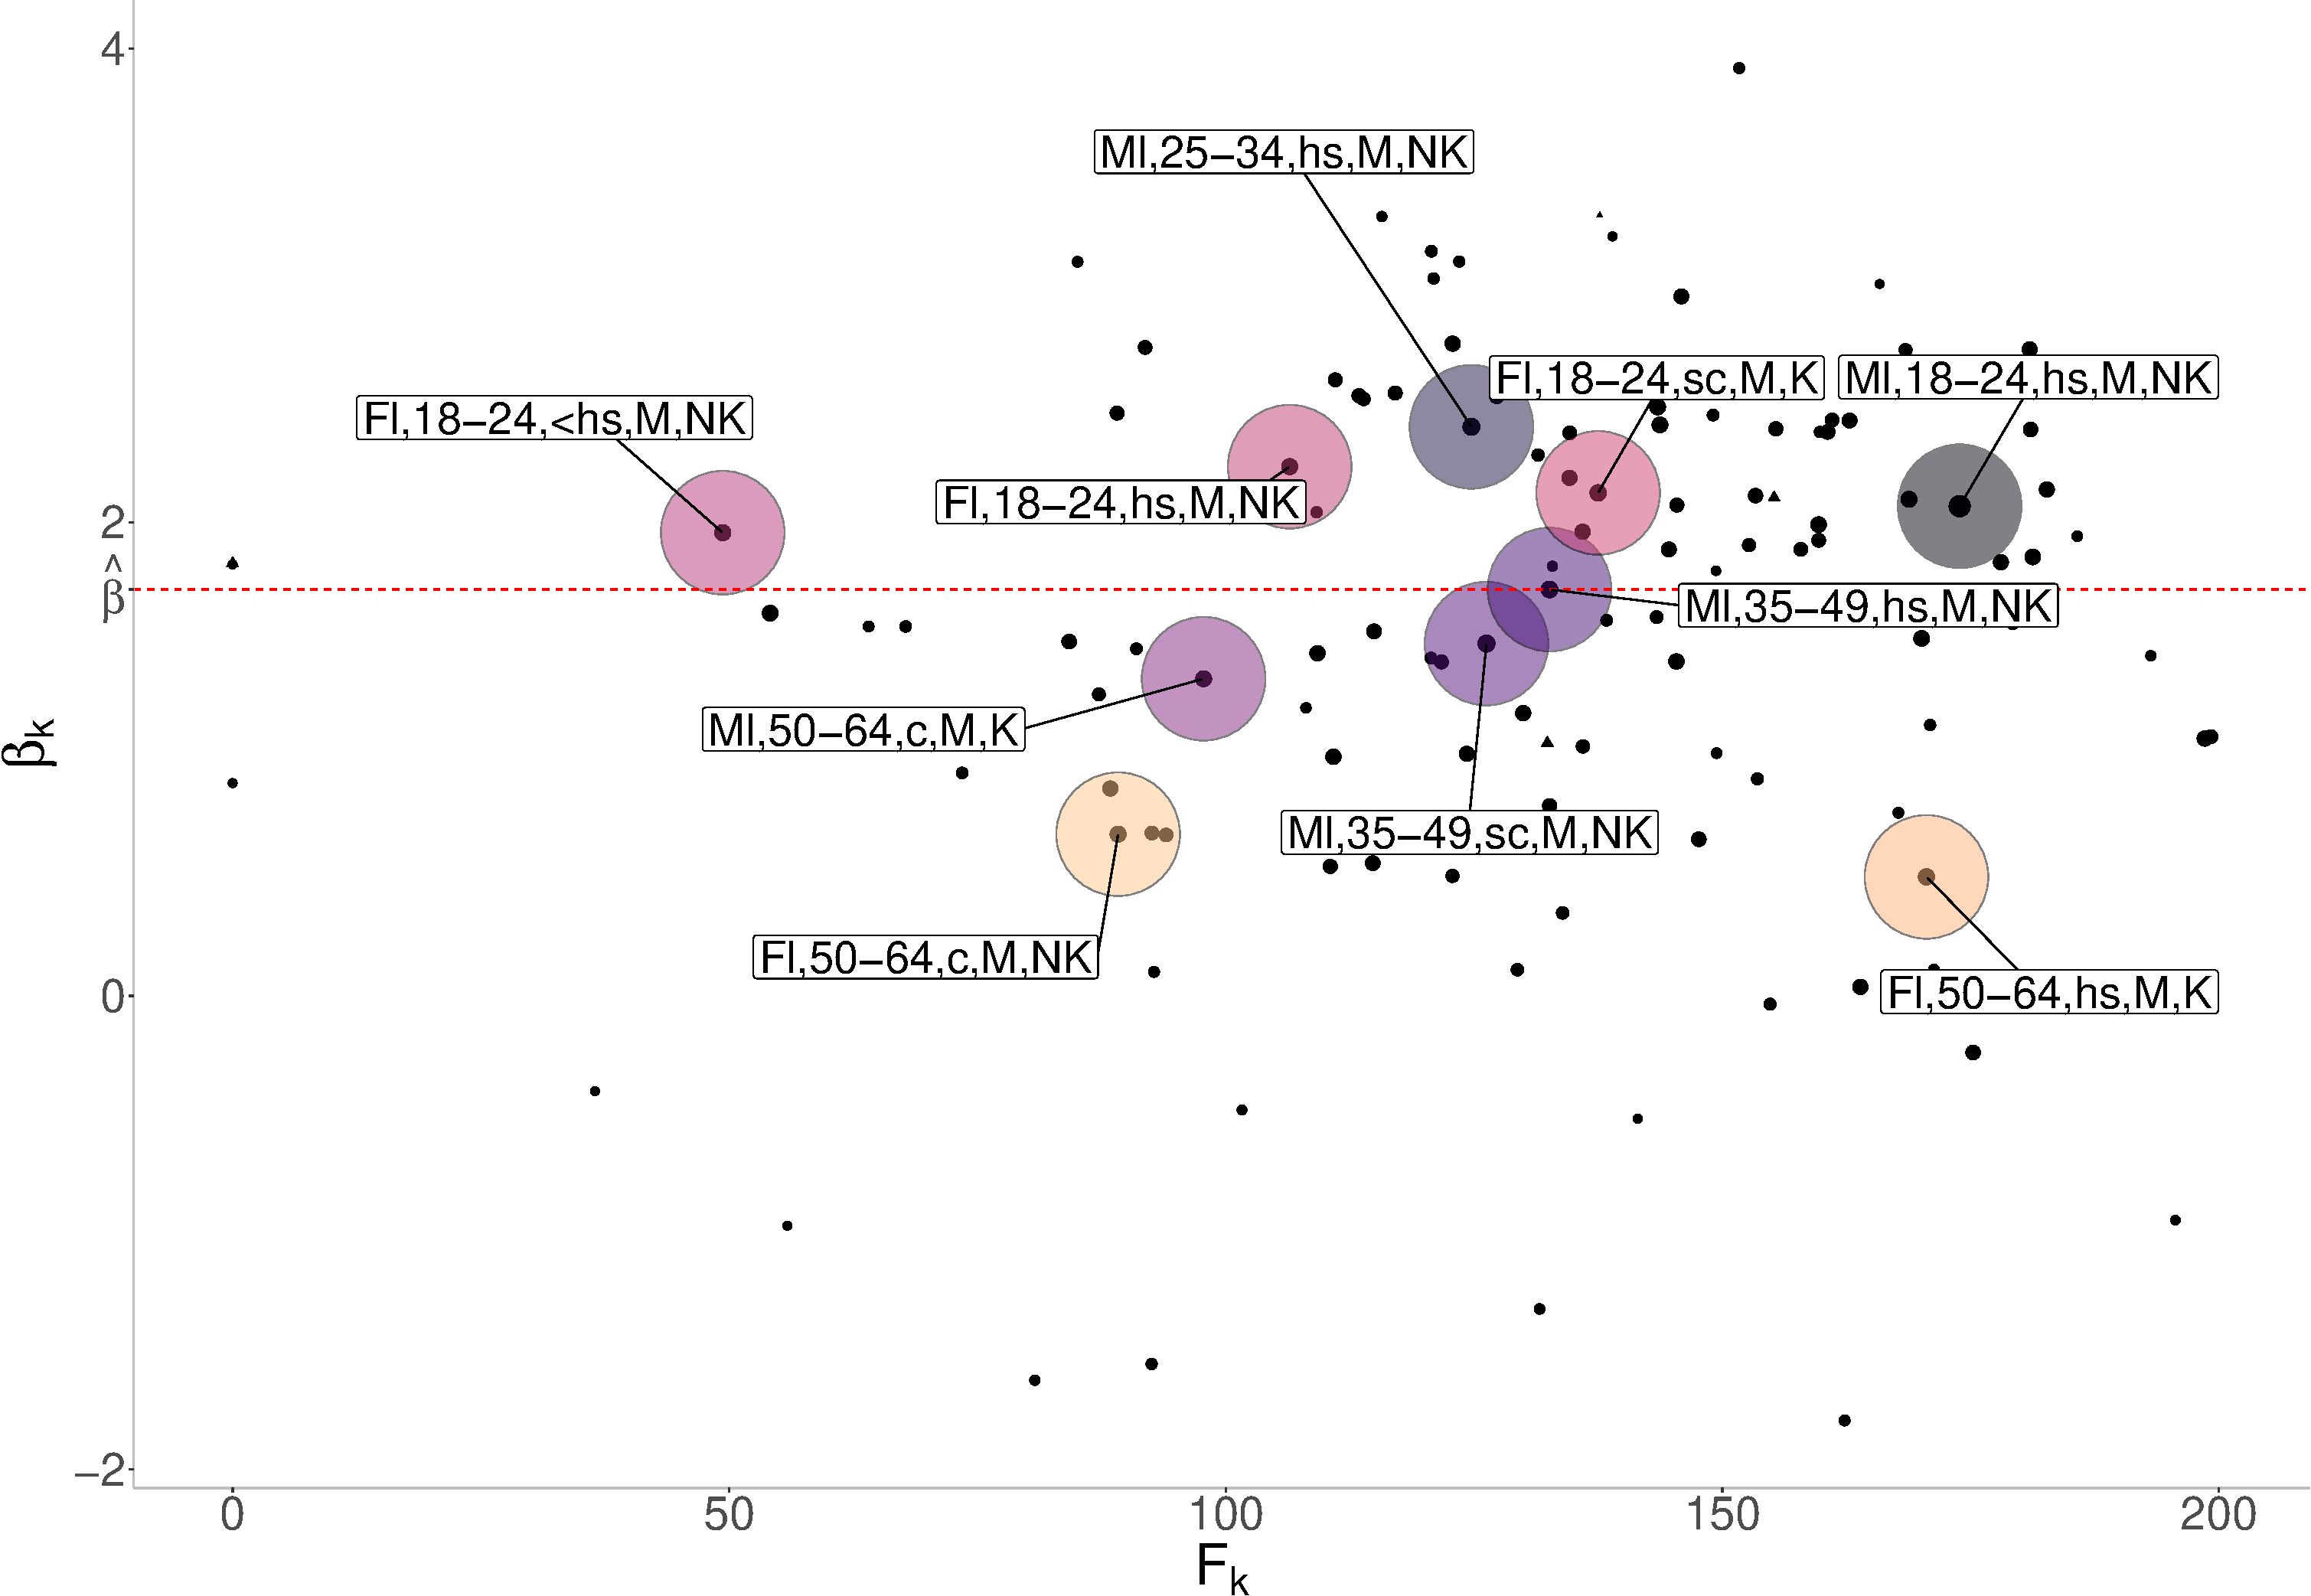
\includegraphics[height=.85\textwidth, width =\textwidth]{figs/weights.pdf}
%\end{figure}

\begin{figure}
\centering
\caption{Estimation weights across groups: michigan shares.}\label{fig:rotweights:group}
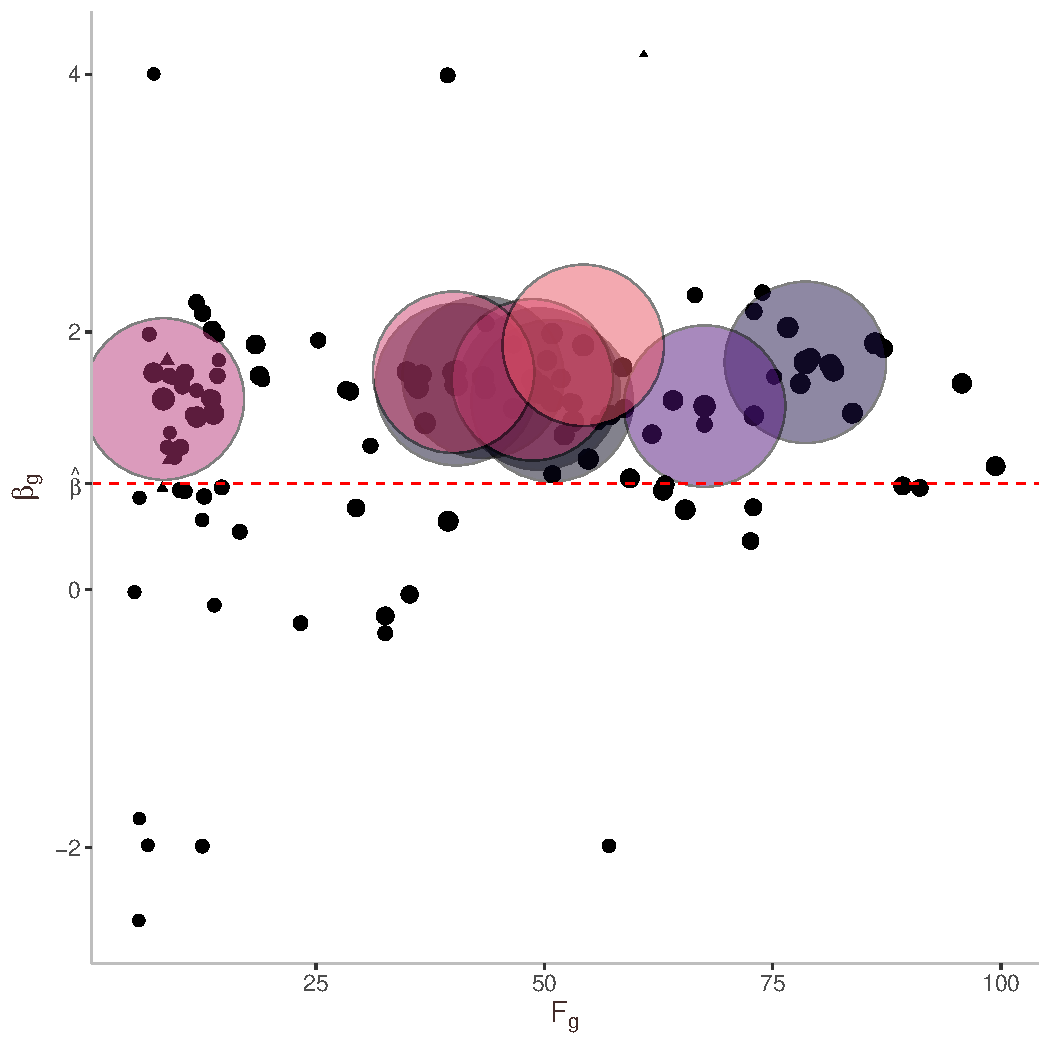
\includegraphics[height=.85\textwidth, width = .85\textwidth]{figs/weightsout}
\end{figure}

\begin{figure}
\centering
\caption{Estimation weights across time.}\label{fig:rotweights:time}
% Created by tikzDevice version 0.12.3.1 on 2023-10-23 16:07:10
% !TEX encoding = UTF-8 Unicode
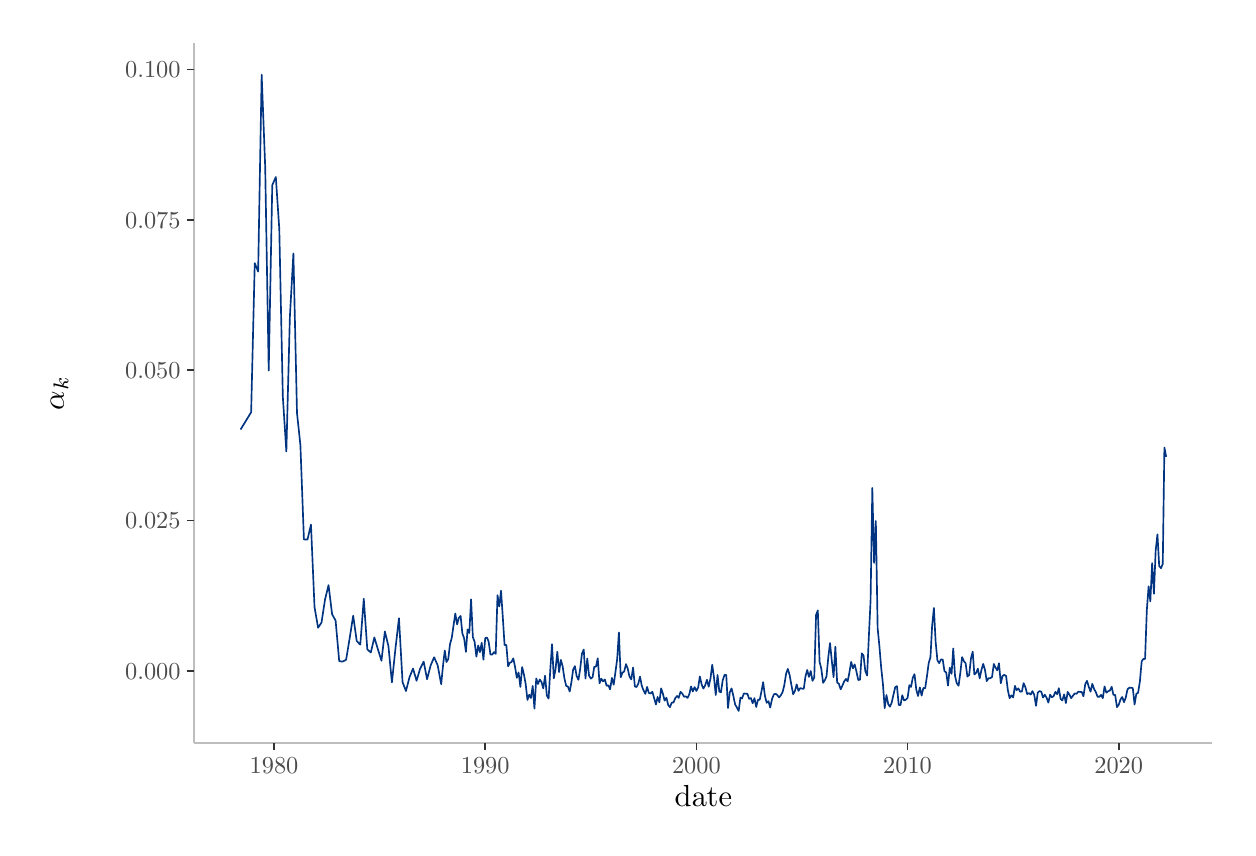
\begin{tikzpicture}[x=1pt,y=1pt]
\definecolor{fillColor}{RGB}{255,255,255}
\path[use as bounding box,fill=fillColor,fill opacity=0.00] (0,0) rectangle (433.62,289.08);
\begin{scope}
\path[clip] (  0.00,  0.00) rectangle (433.62,289.08);
\definecolor{drawColor}{RGB}{255,255,255}
\definecolor{fillColor}{RGB}{255,255,255}

\path[draw=drawColor,line width= 0.6pt,line join=round,line cap=round,fill=fillColor] (  0.00,  0.00) rectangle (433.62,289.08);
\end{scope}
\begin{scope}
\path[clip] ( 60.20, 30.69) rectangle (428.12,283.58);
\definecolor{drawColor}{RGB}{255,255,255}

\path[draw=drawColor,line width= 0.6pt,line join=round] ( 60.20, 56.71) --
	(428.12, 56.71);

\path[draw=drawColor,line width= 0.6pt,line join=round] ( 60.20,111.04) --
	(428.12,111.04);

\path[draw=drawColor,line width= 0.6pt,line join=round] ( 60.20,165.36) --
	(428.12,165.36);

\path[draw=drawColor,line width= 0.6pt,line join=round] ( 60.20,219.69) --
	(428.12,219.69);

\path[draw=drawColor,line width= 0.6pt,line join=round] ( 60.20,274.02) --
	(428.12,274.02);

\path[draw=drawColor,line width= 0.6pt,line join=round] ( 89.02, 30.69) --
	( 89.02,283.58);

\path[draw=drawColor,line width= 0.6pt,line join=round] (165.34, 30.69) --
	(165.34,283.58);

\path[draw=drawColor,line width= 0.6pt,line join=round] (241.63, 30.69) --
	(241.63,283.58);

\path[draw=drawColor,line width= 0.6pt,line join=round] (317.95, 30.69) --
	(317.95,283.58);

\path[draw=drawColor,line width= 0.6pt,line join=round] (394.24, 30.69) --
	(394.24,283.58);
\definecolor{drawColor}{RGB}{0,51,128}

\path[draw=drawColor,line width= 0.6pt,line join=round] ( 76.93,143.87) --
	( 80.75,150.12) --
	( 82.05,203.98) --
	( 83.28,200.96) --
	( 84.55,272.08) --
	( 85.83,238.74) --
	( 87.10,165.19) --
	( 88.38,232.16) --
	( 89.67,235.12) --
	( 90.92,216.35) --
	( 92.20,155.74) --
	( 93.47,135.92) --
	( 94.75,184.70) --
	( 96.02,207.50) --
	( 97.32,149.84) --
	( 98.55,138.20) --
	( 99.82,104.17) --
	(101.10,104.10) --
	(102.37,109.49) --
	(103.65, 79.71) --
	(104.94, 72.25) --
	(106.18, 74.15) --
	(107.45, 82.45) --
	(108.72, 87.65) --
	(110.00, 77.13) --
	(111.27, 74.83) --
	(112.57, 60.20) --
	(113.80, 59.99) --
	(115.07, 60.69) --
	(116.35, 68.46) --
	(117.62, 76.59) --
	(118.90, 67.44) --
	(120.19, 66.14) --
	(121.45, 82.71) --
	(122.72, 64.43) --
	(124.00, 63.30) --
	(125.27, 68.74) --
	(126.54, 64.51) --
	(127.84, 60.33) --
	(129.07, 70.90) --
	(130.35, 65.66) --
	(131.62, 52.49) --
	(132.90, 64.79) --
	(134.17, 75.69) --
	(135.46, 52.58) --
	(136.70, 49.38) --
	(137.97, 54.37) --
	(139.25, 57.49) --
	(140.52, 53.10) --
	(141.79, 57.39) --
	(143.09, 60.00) --
	(144.32, 53.65) --
	(145.60, 58.59) --
	(146.87, 61.58) --
	(148.15, 58.66) --
	(149.42, 51.83) --
	(150.07, 58.46) --
	(150.72, 64.01) --
	(151.32, 59.86) --
	(151.97, 60.90) --
	(152.60, 66.27) --
	(153.24, 68.59) --
	(153.87, 72.95) --
	(154.52, 77.41) --
	(155.17, 73.45) --
	(155.79, 75.79) --
	(156.44, 76.50) --
	(157.07, 70.24) --
	(157.71, 68.39) --
	(158.36, 63.52) --
	(158.95, 71.62) --
	(159.59, 70.36) --
	(160.22, 82.50) --
	(160.87, 68.87) --
	(161.50, 67.15) --
	(162.14, 61.80) --
	(162.79, 65.86) --
	(163.42, 63.43) --
	(164.06, 66.81) --
	(164.69, 60.70) --
	(165.34, 68.55) --
	(165.99, 68.63) --
	(166.57, 67.22) --
	(167.22, 62.56) --
	(167.85, 62.53) --
	(168.49, 63.41) --
	(169.12, 62.82) --
	(169.77, 84.01) --
	(170.42, 79.93) --
	(171.04, 85.63) --
	(171.69, 76.02) --
	(172.32, 66.01) --
	(172.96, 66.03) --
	(173.61, 58.29) --
	(174.20, 59.57) --
	(174.84, 59.84) --
	(175.47, 61.17) --
	(176.12, 58.08) --
	(176.75, 54.14) --
	(177.39, 56.09) --
	(178.04, 50.85) --
	(178.67, 58.04) --
	(179.32, 55.35) --
	(179.94, 51.98) --
	(180.59, 46.15) --
	(181.24, 48.06) --
	(181.84, 46.83) --
	(182.49, 51.22) --
	(183.12, 43.04) --
	(183.77, 53.92) --
	(184.39, 51.90) --
	(185.04, 53.55) --
	(185.69, 52.60) --
	(186.31, 50.33) --
	(186.96, 54.91) --
	(187.59, 47.78) --
	(188.24, 46.63) --
	(188.88, 57.68) --
	(189.47, 66.27) --
	(190.12, 53.95) --
	(190.74, 57.27) --
	(191.39, 63.58) --
	(192.02, 56.23) --
	(192.67, 60.62) --
	(193.31, 58.29) --
	(193.94, 53.99) --
	(194.59, 51.23) --
	(195.21, 51.00) --
	(195.86, 49.18) --
	(196.51, 52.73) --
	(197.09, 57.09) --
	(197.74, 58.38) --
	(198.37, 54.77) --
	(199.02, 53.42) --
	(199.64, 57.33) --
	(200.29, 62.90) --
	(200.94, 64.38) --
	(201.56, 53.92) --
	(202.21, 61.14) --
	(202.84, 54.98) --
	(203.49, 53.87) --
	(204.13, 54.36) --
	(204.72, 58.08) --
	(205.37, 58.22) --
	(205.99, 61.19) --
	(206.64, 52.17) --
	(207.27, 53.81) --
	(207.92, 52.87) --
	(208.56, 53.58) --
	(209.19, 51.28) --
	(209.84, 51.44) --
	(210.46, 49.96) --
	(211.11, 54.12) --
	(211.76, 51.68) --
	(212.37, 56.10) --
	(213.01, 60.90) --
	(213.64, 70.53) --
	(214.29, 54.35) --
	(214.91, 55.99) --
	(215.56, 56.47) --
	(216.21, 59.11) --
	(216.84, 57.42) --
	(217.48, 54.53) --
	(218.11, 53.58) --
	(218.76, 57.85) --
	(219.41, 51.04) --
	(219.99, 50.80) --
	(220.64, 52.01) --
	(221.27, 54.58) --
	(221.91, 51.25) --
	(222.54, 49.64) --
	(223.19, 48.33) --
	(223.83, 50.85) --
	(224.46, 48.64) --
	(225.11, 48.50) --
	(225.74, 49.10) --
	(226.38, 46.76) --
	(227.03, 44.51) --
	(227.62, 47.24) --
	(228.26, 45.33) --
	(228.89, 50.34) --
	(229.54, 48.39) --
	(230.16, 45.91) --
	(230.81, 46.97) --
	(231.46, 44.30) --
	(232.09, 43.56) --
	(232.73, 45.19) --
	(233.36, 45.24) --
	(234.01, 46.80) --
	(234.66, 47.58) --
	(235.24, 46.92) --
	(235.89, 49.06) --
	(236.52, 48.50) --
	(237.16, 47.32) --
	(237.79, 47.45) --
	(238.44, 46.88) --
	(239.09, 48.25) --
	(239.71, 51.02) --
	(240.36, 49.21) --
	(240.99, 50.80) --
	(241.63, 49.41) --
	(242.28, 50.63) --
	(242.89, 54.67) --
	(243.54, 51.75) --
	(244.16, 50.25) --
	(244.81, 51.42) --
	(245.44, 53.44) --
	(246.08, 50.95) --
	(246.73, 53.93) --
	(247.36, 58.88) --
	(248.01, 54.20) --
	(248.63, 47.94) --
	(249.28, 55.15) --
	(249.93, 49.17) --
	(250.51, 48.91) --
	(251.16, 53.30) --
	(251.79, 55.20) --
	(252.43, 55.18) --
	(253.06, 43.23) --
	(253.71, 48.97) --
	(254.36, 50.34) --
	(254.98, 47.67) --
	(255.63, 44.51) --
	(256.26, 43.46) --
	(256.91, 42.18) --
	(257.55, 47.01) --
	(258.14, 46.68) --
	(258.79, 48.49) --
	(259.41, 48.42) --
	(260.06, 48.41) --
	(260.69, 46.58) --
	(261.33, 46.84) --
	(261.98, 44.95) --
	(262.61, 46.81) --
	(263.26, 43.62) --
	(263.88, 46.19) --
	(264.53, 46.23) --
	(265.18, 49.37) --
	(265.76, 52.58) --
	(266.41, 47.59) --
	(267.04, 45.12) --
	(267.69, 45.69) --
	(268.31, 43.39) --
	(268.96, 46.45) --
	(269.61, 48.12) --
	(270.23, 48.40) --
	(270.88, 47.92) --
	(271.51, 47.06) --
	(272.16, 47.83) --
	(272.80, 49.04) --
	(273.41, 51.54) --
	(274.06, 55.68) --
	(274.68, 57.37) --
	(275.33, 55.15) --
	(275.96, 51.60) --
	(276.61, 48.20) --
	(277.25, 49.43) --
	(277.88, 51.76) --
	(278.53, 49.44) --
	(279.15, 50.42) --
	(279.80, 50.24) --
	(280.45, 50.19) --
	(281.04, 54.57) --
	(281.68, 56.99) --
	(282.31, 54.49) --
	(282.96, 56.60) --
	(283.58, 53.06) --
	(284.23, 54.25) --
	(284.88, 76.85) --
	(285.51, 78.51) --
	(286.15, 59.96) --
	(286.78, 57.38) --
	(287.43, 52.34) --
	(288.08, 53.34) --
	(288.66, 54.67) --
	(289.31, 61.69) --
	(289.93, 66.70) --
	(290.58, 60.20) --
	(291.21, 54.39) --
	(291.86, 65.42) --
	(292.50, 52.45) --
	(293.13, 51.99) --
	(293.78, 50.00) --
	(294.41, 51.39) --
	(295.05, 52.87) --
	(295.70, 53.75) --
	(296.29, 52.85) --
	(296.93, 56.08) --
	(297.56, 59.90) --
	(298.21, 57.59) --
	(298.83, 58.99) --
	(299.48, 56.37) --
	(300.13, 53.36) --
	(300.76, 53.47) --
	(301.40, 63.00) --
	(302.03, 62.22) --
	(302.68, 56.58) --
	(303.33, 54.97) --
	(303.93, 68.43) --
	(304.58, 82.16) --
	(305.21,122.77) --
	(305.85, 95.69) --
	(306.48,110.82) --
	(307.13, 72.15) --
	(307.78, 65.47) --
	(308.40, 57.95) --
	(309.05, 51.82) --
	(309.68, 43.21) --
	(310.32, 47.92) --
	(310.97, 44.60) --
	(311.56, 43.73) --
	(312.20, 45.14) --
	(312.83, 47.97) --
	(313.48, 50.77) --
	(314.11, 51.13) --
	(314.75, 44.36) --
	(315.40, 44.33) --
	(316.03, 47.85) --
	(316.68, 45.98) --
	(317.30, 46.21) --
	(317.95, 46.89) --
	(318.60, 51.49) --
	(319.18, 50.84) --
	(319.83, 54.17) --
	(320.46, 55.45) --
	(321.10, 49.86) --
	(321.73, 47.58) --
	(322.38, 50.66) --
	(323.03, 47.74) --
	(323.65, 50.46) --
	(324.30, 50.37) --
	(324.93, 54.57) --
	(325.58, 59.46) --
	(326.22, 61.62) --
	(326.81, 72.76) --
	(327.46, 79.39) --
	(328.08, 67.27) --
	(328.73, 60.43) --
	(329.36, 59.46) --
	(330.00, 60.78) --
	(330.65, 60.73) --
	(331.28, 56.57) --
	(331.93, 56.06) --
	(332.55, 51.33) --
	(333.20, 57.80) --
	(333.85, 55.60) --
	(334.45, 64.74) --
	(335.10, 54.76) --
	(335.73, 52.18) --
	(336.38, 51.29) --
	(337.00, 55.86) --
	(337.65, 61.63) --
	(338.30, 60.14) --
	(338.92, 59.43) --
	(339.57, 54.59) --
	(340.20, 55.17) --
	(340.85, 61.12) --
	(341.49, 63.61) --
	(342.08, 55.36) --
	(342.73, 55.93) --
	(343.35, 57.47) --
	(344.00, 53.95) --
	(344.63, 56.94) --
	(345.28, 59.19) --
	(345.92, 57.03) --
	(346.55, 52.97) --
	(347.20, 53.98) --
	(347.82, 54.01) --
	(348.47, 54.46) --
	(349.12, 59.16) --
	(349.70, 57.92) --
	(350.35, 56.85) --
	(350.98, 59.40) --
	(351.63, 52.17) --
	(352.25, 54.80) --
	(352.90, 55.22) --
	(353.55, 54.82) --
	(354.18, 49.71) --
	(354.82, 46.79) --
	(355.45, 47.80) --
	(356.10, 47.04) --
	(356.75, 51.24) --
	(357.33, 49.67) --
	(357.98, 50.34) --
	(358.60, 49.14) --
	(359.25, 49.17) --
	(359.88, 52.22) --
	(360.53, 50.72) --
	(361.17, 48.26) --
	(361.80, 48.62) --
	(362.45, 48.12) --
	(363.08, 49.35) --
	(363.72, 47.99) --
	(364.37, 44.03) --
	(364.98, 48.76) --
	(365.62, 49.37) --
	(366.25, 49.16) --
	(366.90, 47.03) --
	(367.52, 48.03) --
	(368.17, 46.99) --
	(368.82, 45.17) --
	(369.45, 48.04) --
	(370.09, 47.11) --
	(370.72, 47.55) --
	(371.37, 49.07) --
	(372.02, 48.21) --
	(372.60, 50.39) --
	(373.25, 46.49) --
	(373.88, 45.99) --
	(374.52, 48.17) --
	(375.15, 45.03) --
	(375.80, 49.04) --
	(376.45, 48.01) --
	(377.07, 46.82) --
	(377.72, 47.71) --
	(378.35, 48.49) --
	(378.99, 48.38) --
	(379.64, 49.14) --
	(380.23, 49.05) --
	(380.87, 49.06) --
	(381.50, 47.48) --
	(382.15, 51.87) --
	(382.78, 53.07) --
	(383.42, 50.92) --
	(384.07, 49.12) --
	(384.70, 51.97) --
	(385.35, 50.12) --
	(385.97, 48.99) --
	(386.62, 47.28) --
	(387.27, 47.31) --
	(387.85, 47.98) --
	(388.50, 46.79) --
	(389.13, 51.03) --
	(389.77, 48.77) --
	(390.40, 49.28) --
	(391.05, 49.55) --
	(391.70, 50.90) --
	(392.32, 48.00) --
	(392.97, 47.93) --
	(393.60, 43.55) --
	(394.24, 44.40) --
	(394.89, 46.34) --
	(395.50, 47.23) --
	(396.15, 45.34) --
	(396.77, 46.98) --
	(397.42, 50.01) --
	(398.05, 50.57) --
	(398.69, 50.59) --
	(399.34, 50.41) --
	(399.97, 44.52) --
	(400.62, 48.39) --
	(401.24, 48.72) --
	(401.89, 52.80) --
	(402.54, 60.05) --
	(403.12, 60.94) --
	(403.77, 60.99) --
	(404.40, 78.59) --
	(405.05, 87.21) --
	(405.67, 81.77) --
	(406.32, 95.58) --
	(406.97, 84.53) --
	(407.59,100.06) --
	(408.24,105.98) --
	(408.87, 94.55) --
	(409.52, 93.76) --
	(410.16, 95.31) --
	(410.75,137.35) --
	(411.40,134.00);
\end{scope}
\begin{scope}
\path[clip] (  0.00,  0.00) rectangle (433.62,289.08);
\definecolor{drawColor}{RGB}{190,190,190}

\path[draw=drawColor,line width= 0.6pt,line join=round] ( 60.20, 30.69) --
	( 60.20,283.58);
\end{scope}
\begin{scope}
\path[clip] (  0.00,  0.00) rectangle (433.62,289.08);
\definecolor{drawColor}{gray}{0.30}

\node[text=drawColor,anchor=base east,inner sep=0pt, outer sep=0pt, scale=  0.88] at ( 55.25, 53.68) {0.000};

\node[text=drawColor,anchor=base east,inner sep=0pt, outer sep=0pt, scale=  0.88] at ( 55.25,108.01) {0.025};

\node[text=drawColor,anchor=base east,inner sep=0pt, outer sep=0pt, scale=  0.88] at ( 55.25,162.33) {0.050};

\node[text=drawColor,anchor=base east,inner sep=0pt, outer sep=0pt, scale=  0.88] at ( 55.25,216.66) {0.075};

\node[text=drawColor,anchor=base east,inner sep=0pt, outer sep=0pt, scale=  0.88] at ( 55.25,270.99) {0.100};
\end{scope}
\begin{scope}
\path[clip] (  0.00,  0.00) rectangle (433.62,289.08);
\definecolor{drawColor}{gray}{0.20}

\path[draw=drawColor,line width= 0.6pt,line join=round] ( 57.45, 56.71) --
	( 60.20, 56.71);

\path[draw=drawColor,line width= 0.6pt,line join=round] ( 57.45,111.04) --
	( 60.20,111.04);

\path[draw=drawColor,line width= 0.6pt,line join=round] ( 57.45,165.36) --
	( 60.20,165.36);

\path[draw=drawColor,line width= 0.6pt,line join=round] ( 57.45,219.69) --
	( 60.20,219.69);

\path[draw=drawColor,line width= 0.6pt,line join=round] ( 57.45,274.02) --
	( 60.20,274.02);
\end{scope}
\begin{scope}
\path[clip] (  0.00,  0.00) rectangle (433.62,289.08);
\definecolor{drawColor}{RGB}{190,190,190}

\path[draw=drawColor,line width= 0.6pt,line join=round] ( 60.20, 30.69) --
	(428.12, 30.69);
\end{scope}
\begin{scope}
\path[clip] (  0.00,  0.00) rectangle (433.62,289.08);
\definecolor{drawColor}{gray}{0.20}

\path[draw=drawColor,line width= 0.6pt,line join=round] ( 89.02, 27.94) --
	( 89.02, 30.69);

\path[draw=drawColor,line width= 0.6pt,line join=round] (165.34, 27.94) --
	(165.34, 30.69);

\path[draw=drawColor,line width= 0.6pt,line join=round] (241.63, 27.94) --
	(241.63, 30.69);

\path[draw=drawColor,line width= 0.6pt,line join=round] (317.95, 27.94) --
	(317.95, 30.69);

\path[draw=drawColor,line width= 0.6pt,line join=round] (394.24, 27.94) --
	(394.24, 30.69);
\end{scope}
\begin{scope}
\path[clip] (  0.00,  0.00) rectangle (433.62,289.08);
\definecolor{drawColor}{gray}{0.30}

\node[text=drawColor,anchor=base,inner sep=0pt, outer sep=0pt, scale=  0.88] at ( 89.02, 19.68) {1980};

\node[text=drawColor,anchor=base,inner sep=0pt, outer sep=0pt, scale=  0.88] at (165.34, 19.68) {1990};

\node[text=drawColor,anchor=base,inner sep=0pt, outer sep=0pt, scale=  0.88] at (241.63, 19.68) {2000};

\node[text=drawColor,anchor=base,inner sep=0pt, outer sep=0pt, scale=  0.88] at (317.95, 19.68) {2010};

\node[text=drawColor,anchor=base,inner sep=0pt, outer sep=0pt, scale=  0.88] at (394.24, 19.68) {2020};
\end{scope}
\begin{scope}
\path[clip] (  0.00,  0.00) rectangle (433.62,289.08);
\definecolor{drawColor}{RGB}{0,0,0}

\node[text=drawColor,anchor=base,inner sep=0pt, outer sep=0pt, scale=  1.10] at (244.16,  7.64) {date};
\end{scope}
\begin{scope}
\path[clip] (  0.00,  0.00) rectangle (433.62,289.08);
\definecolor{drawColor}{RGB}{0,0,0}

\node[text=drawColor,rotate= 90.00,anchor=base,inner sep=0pt, outer sep=0pt, scale=  1.10] at ( 13.08,157.13) {$\alpha_{k}$};
\end{scope}
\end{tikzpicture}

\end{figure}

\begin{table}

\caption{\label{tab:rotweights:groups}Group weights}
\centering
\resizebox{\linewidth}{!}{
\begin{threeparttable}
\begin{tabular}[t]{cccccccccc}
\toprule
shares & men & women & ages 18-24 & ages 25-34 & ages 35-49 & ages 50-64 & ages 65+ & w/h.s. degree & w/college+ degree\\
\midrule
\cellcolor{gray!6}{cps} & \cellcolor{gray!6}{0.5271} & \cellcolor{gray!6}{0.4729} & \cellcolor{gray!6}{0.2445} & \cellcolor{gray!6}{0.3488} & \cellcolor{gray!6}{0.2767} & \cellcolor{gray!6}{0.0935} & \cellcolor{gray!6}{0.0364} & \cellcolor{gray!6}{0.3476} & \cellcolor{gray!6}{0.4132}\\
\addlinespace
michigan & 0.5669 & 0.4331 & 0.3466 & 0.3097 & 0.1565 & 0.1189 & 0.0682 & 0.2924 & 0.2792\\
\bottomrule
\end{tabular}
\begin{tablenotes}
\item \textit{Note: } 
\item Calculates fraction of Rotemberg weights associated with broad groups: CPS shares.
\end{tablenotes}
\end{threeparttable}}
\end{table}


\subsection{Alternative estimates}

As previously mentioned, there are potential concerns with the data. Table \ref{tab:table:2sls:robust} presents alternative estimates that address these concerns. Throughout, the Bartik instrument uses Michigan survey shares.

\begin{table}

\caption{\label{tab:table:2sls:robust}Alternative estimates}
\centering
\resizebox{\linewidth}{!}{
\begin{threeparttable}
\begin{tabular}[t]{lllll}
\toprule
  & small & first-only & state-CPI & lag michigan shares\\
\midrule
\cellcolor{gray!6}{Dependent Var.:} & \cellcolor{gray!6}{RegInf} & \cellcolor{gray!6}{RegInf} & \cellcolor{gray!6}{RegInf} & \cellcolor{gray!6}{RegInf}\\
\addlinespace
 &  &  &  & \\
\addlinespace
\cellcolor{gray!6}{pe} & \cellcolor{gray!6}{0.6618** (0.2540)} & \cellcolor{gray!6}{0.5811 (0.4747)} & \cellcolor{gray!6}{0.3340* (0.1490)} & \cellcolor{gray!6}{0.5313* (0.2503)}\\
\addlinespace
Controls & Yes & Yes & Yes & Yes\\
\addlinespace
\cellcolor{gray!6}{Fixed-Effects:} & \cellcolor{gray!6}{-----------------} & \cellcolor{gray!6}{---------------} & \cellcolor{gray!6}{----------------} & \cellcolor{gray!6}{----------------}\\
\addlinespace
REGION & Yes & Yes & Yes & Yes\\
\addlinespace
\cellcolor{gray!6}{TIME} & \cellcolor{gray!6}{Yes} & \cellcolor{gray!6}{Yes} & \cellcolor{gray!6}{Yes} & \cellcolor{gray!6}{Yes}\\
\addlinespace
\_\_\_\_\_\_\_\_\_\_\_\_\_\_\_ & \_\_\_\_\_\_\_\_\_\_\_\_\_\_\_\_\_ & \_\_\_\_\_\_\_\_\_\_\_\_\_\_\_ & \_\_\_\_\_\_\_\_\_\_\_\_\_\_\_\_ & \_\_\_\_\_\_\_\_\_\_\_\_\_\_\_\_\\
\addlinespace
\cellcolor{gray!6}{S.E. type} & \cellcolor{gray!6}{Drisc.-Kra. (L=4)} & \cellcolor{gray!6}{Dri.-Kra. (L=4)} & \cellcolor{gray!6}{Dris.-Kra. (L=4)} & \cellcolor{gray!6}{Dris.-Kra. (L=4)}\\
\addlinespace
Observations & 1,387 & 1,387 & 1,427 & 1,387\\
\addlinespace
\cellcolor{gray!6}{R2} & \cellcolor{gray!6}{0.93371} & \cellcolor{gray!6}{0.91353} & \cellcolor{gray!6}{0.95314} & \cellcolor{gray!6}{0.94105}\\
\addlinespace
Within R2 & 0.35786 & 0.16236 & 0.56477 & 0.42896\\
\bottomrule
\end{tabular}
\begin{tablenotes}
\item \textit{Note: } 
\item ``small'' removes large survey responses.  ``first'' includes only first-time survey respondents.  ``state-cpi'' measures regional inflation by aggregating state-level CPI's.  ``lag michigan shares'' instruments with 12 month lagged survey shares.
\end{tablenotes}
\end{threeparttable}}
\end{table}



The first two columns filter out specific survey responses. The first column, labeled ``small'', removes outliers from the empirical analysis. In particular, survey forecasts that are greater than $\pm 25\%$. The estimated effect is stronger than the baseline and still significant at the 1\% level. The estimate without outliers is not preferred, however, as there is not a good reason to omit survey expectations that are large in magnitude. Strong responses to subjective beliefs could significantly impact those consumers' behavior. The second column (``first-only'') removes those survey respondents interviewed for a second time, roughly 40\% of the sample. The concern is that these respondents differ from those participating the first time. While the estimate is still significant, the effect size is close to the OLS estimate.

The final two columns in Table \ref{tab:table:2sls:robust} construct the dependent variable and instrument differently. The third column (``state-CPI'') constructs the regional inflation measure using the state CPI measures developed by \cite{NakamuraSteinsson:QJE2022}. The regional CPI measures from the BLS are monthly for a shorter period than the length of the Michigan survey. The regional inflation constructed by state-level CPI aligns with the sample periods. A regional CPI emerges as a weighted average of the CPI for each state in a region, where the weights are the state's consumer expenditure share in the region. One downside to this alternative inflation measure is that the state level CPI's in \cite{NakamuraSteinsson:QJE2022} do not include all of the states in each region for the entire sample requiring some interpolation. Table \ref{tab:table:2sls:robust} illustrates that the alternative regional inflation measure does not impact estimation. Finally, the last column instruments for inflation expectations with a twelve-month lag of Michigan shares. If one is concerned that the contemporaneous Michigan survey measures -- meant to be nationally representative by the survey design -- may not be strictly exogenous. However, the CPS 1978.1 population shares being time-invariant, the lagged share measure is a compromise. The effect lies in the middle of the baseline estimates, as expected.



\section{Impact of five-year ahead inflation expectations}


Having quantified the impact of one-year ahead inflation expectations on regional inflation rates, let us measure the relative contributions of short versus long-run expectations. The Michigan survey also asks consumers about their expectations of inflation over the ``next 5-10 years.'' 

Figure \ref{fig:5year:redform} plots the corresponding reduced-form estimates for long-run expectations. Instrumenting is now for both short- and long-run expectations, using the Michigan survey shares and the CPS 1978.1. The top panel plots the 5-10 year Bartik instrument against 5-10 year ahead inflation expectations. As before, the instrument correlates tightly with long-horizon expectations. The bottom panel plots the reduced-form regression of regional inflation on the long-horizon instrument. Here that relationship is negative, and the slope of the regression line is flat.  


\begin{figure}
\centering
\caption{Long-run inflation expectations: reduced-form estimates.}\label{fig:5year:redform}
\begin{subfigure}[t]{0.75\textwidth}
\centering
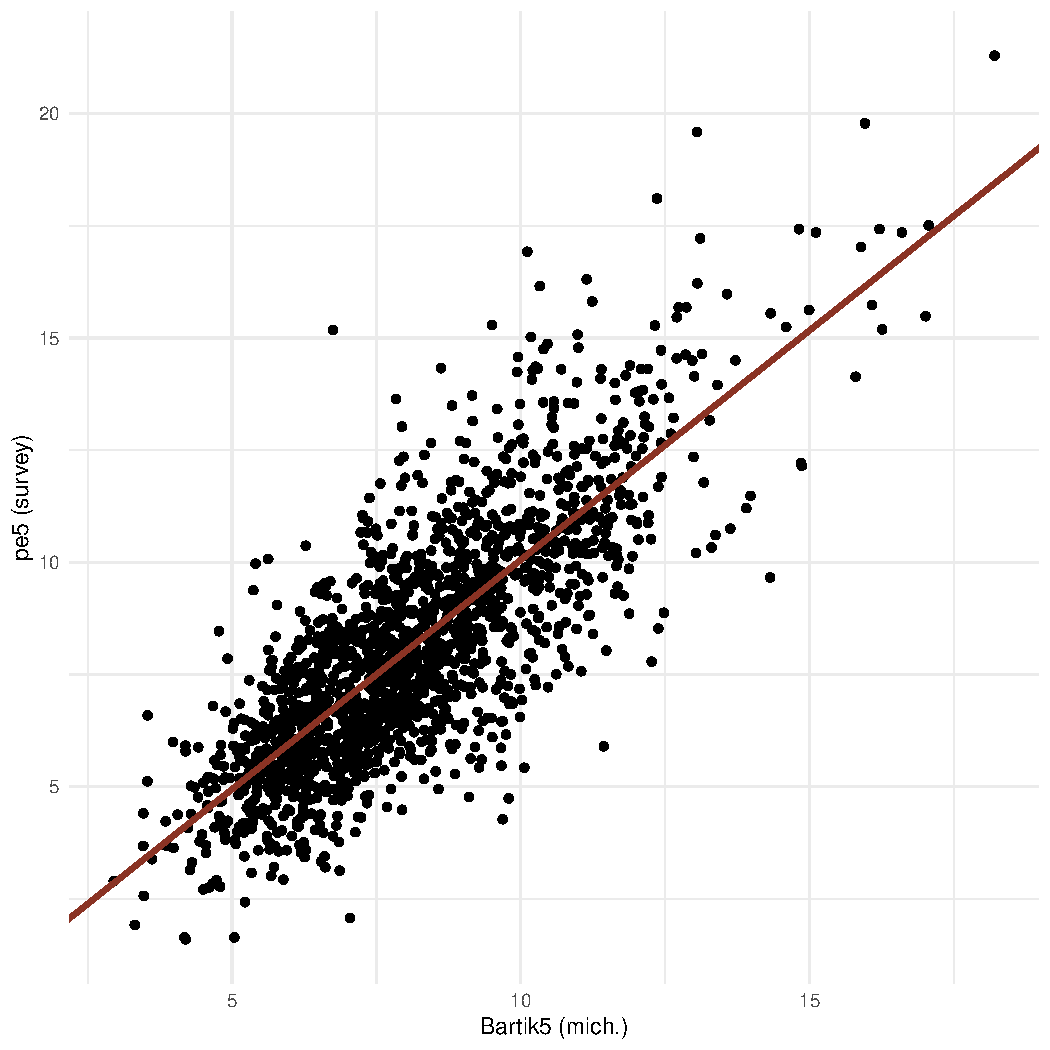
\includegraphics[width = 5in, height =3in]{figs/firstStage5only}
\caption{First stage long-horizon expectations only.  }\label{5yearsubfig:shares:group}
\end{subfigure}
\vfill
\begin{subfigure}[t]{0.75\textwidth}
\centering
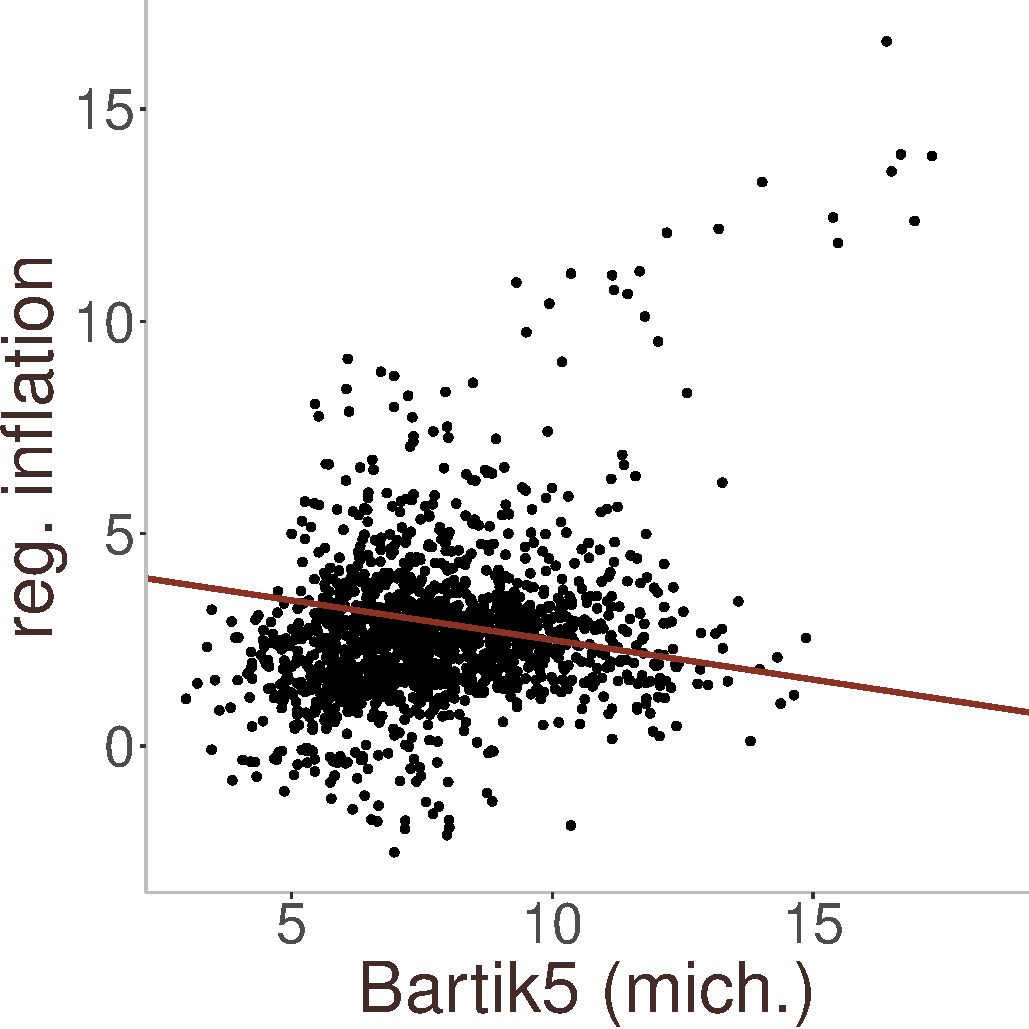
\includegraphics[width =5in, height =3in]{figs/redform5only}
\caption{Reduced form long-horizon expectations only.}\label{5yearsubfig:shares:cps}
\end{subfigure}
\end{figure}

The 2sls estimates in Tables \ref{tab:2sls:shortandlong:stage1}-\ref{tab:2sls:shortandlong:stage2} confirm the reduced-form findings. In the first stage, the short- and long-run instruments are relevant for short- and long-term inflation, respectively. The long-horizon instrument has no predictive power for short-run expectations. In the second stage (Table \ref{tab:2sls:shortandlong:stage2}), the coefficient estimates on short-run expectations are virtually identical to the preferred estimates. Long-horizon expectations have a small negative impact that is not statistically significant.  

\begin{landscape}
\begin{table}[!htbp] \centering
\caption{2SLS with short and long expectations: first stage}
\label{tab:table:2sls:shortlong:stage1}
\textbf{Panel A: CPS shares} \\ 
\begin{tabular}[t]{>{}llccccccc}
\toprule
  & (1)-pe & (1)-pe5 & (2)-pe & (2)-pe5 & (3)-pe & (3)-pe5 & (4)-pe & (4)-pe5\\
\midrule
\textbf{\cellcolor{gray!10}{Cf.}} & \cellcolor{gray!10}{0.43 (0.03)} & \cellcolor{gray!10}{-0.27 (0.1)} & \cellcolor{gray!10}{1.35 (0.09)} & \cellcolor{gray!10}{0.65 (0.11)} & \cellcolor{gray!10}{1.48 (0.03)} & \cellcolor{gray!10}{0.62 (0.11)} & \cellcolor{gray!10}{0.26 (0.13)} & \cellcolor{gray!10}{-0.24 (0.1)}\\
\textbf{$R^2$} & 0.80 & 0.40 & 0.68 & 0.18 & 0.72 & 0.19 & 0.78 & 0.38\\
\textbf{\cellcolor{gray!10}{F}} & \cellcolor{gray!10}{12.17} & \cellcolor{gray!10}{4.13} & \cellcolor{gray!10}{261.22} & \cellcolor{gray!10}{46.66} & \cellcolor{gray!10}{315.11} & \cellcolor{gray!10}{45.74} & \cellcolor{gray!10}{5.37} & \cellcolor{gray!10}{4.43}\\
\bottomrule
\end{tabular} \vspace{5mm} 
\\ \textbf{Panel B: Michigan shares} \\ 
\begin{tabular}[t]{>{}llccccccc}
\toprule
  & (1)-pe & (1)-pe5 & (2)-pe & (2)-pe5 & (3)-pe & (3)-pe5 & (4)-pe & (4)-pe5\\
\midrule
\textbf{\cellcolor{gray!10}{Cf.}} & \cellcolor{gray!10}{0.24 (0.02)} & \cellcolor{gray!10}{-0.17 (0.06)} & \cellcolor{gray!10}{0.75 (0.02)} & \cellcolor{gray!10}{0.33 (0.04)} & \cellcolor{gray!10}{0.74 (0.02)} & \cellcolor{gray!10}{0.35 (0.04)} & \cellcolor{gray!10}{0.23 (0.02)} & \cellcolor{gray!10}{-0.19 (0.05)}\\
\textbf{$R^2$} & 0.80 & 0.40 & 0.72 & 0.18 & 0.74 & 0.19 & 0.79 & 0.39\\
\textbf{\cellcolor{gray!10}{F}} & \cellcolor{gray!10}{17.17} & \cellcolor{gray!10}{6.64} & \cellcolor{gray!10}{372.11} & \cellcolor{gray!10}{42.85} & \cellcolor{gray!10}{384.19} & \cellcolor{gray!10}{45.73} & \cellcolor{gray!10}{15.48} & \cellcolor{gray!10}{8.90}\\
\bottomrule
\end{tabular}\end{table}
\end{landscape}


\begin{table}

\caption{\label{tab:2sls:shortandlong:stage2}2SLS with short and long-expectations: coefficient estimates}
\centering
\begin{threeparttable}
\begin{tabular}[t]{lll}
\toprule
  & survey & CPS78\\
\midrule
\cellcolor{gray!6}{Dependent Var.:} & \cellcolor{gray!6}{RegInf} & \cellcolor{gray!6}{RegInf}\\
\addlinespace
 &  & \\
\addlinespace
\cellcolor{gray!6}{short-run pe} & \cellcolor{gray!6}{0.3355* (0.1475)} & \cellcolor{gray!6}{0.5394** (0.1931)}\\
\addlinespace
long-run pe & -0.0228 (0.0450) & -0.0373 (0.0746)\\
\addlinespace
\cellcolor{gray!6}{Controls} & \cellcolor{gray!6}{Yes} & \cellcolor{gray!6}{Yes}\\
\addlinespace
Fixed-Effects: & ---------------- & -----------------\\
\addlinespace
\cellcolor{gray!6}{REGION} & \cellcolor{gray!6}{Yes} & \cellcolor{gray!6}{Yes}\\
\addlinespace
TIME & Yes & Yes\\
\addlinespace
\cellcolor{gray!6}{\_\_\_\_\_\_\_\_\_\_\_\_\_\_\_} & \cellcolor{gray!6}{\_\_\_\_\_\_\_\_\_\_\_\_\_\_\_\_} & \cellcolor{gray!6}{\_\_\_\_\_\_\_\_\_\_\_\_\_\_\_\_\_}\\
\addlinespace
S.E. type & Dris.-Kra. (L=4) & Drisc.-Kra. (L=4)\\
\addlinespace
\cellcolor{gray!6}{Observations} & \cellcolor{gray!6}{1,387} & \cellcolor{gray!6}{1,387}\\
\addlinespace
R2 & 0.95325 & 0.93851\\
\addlinespace
\cellcolor{gray!6}{Within R2} & \cellcolor{gray!6}{0.54716} & \cellcolor{gray!6}{0.40438}\\
\bottomrule
\end{tabular}
\begin{tablenotes}
\item \textit{Note: } 
\item Survey is the benchmark shift-share instrument using Michigan survey shares. CPS78 is constructed from the 1978.1 CPS.
\end{tablenotes}
\end{threeparttable}
\end{table}


One might wonder if long-horizon expectations can ever proxy for short-run expectations and identify an effect acting on inflation.  Tables \ref{tab:2sls:long:stage1}-\ref{tab:2sls:long:stage2} show that, again, there is no effect running from long-horizon expectations to inflation.  While the estimated sign for long-horizon expectations is again positive, it is close to zero and insignificant.  

\begin{table}

\caption{\label{tab:2sls:long:stage1}2SLS with long-expectations: first stage}
\centering
\begin{threeparttable}
\begin{tabular}[t]{lll}
\toprule
  & survey long pe & CPS78 long pe\\
\midrule
\cellcolor{gray!6}{Dependent Var.:} & \cellcolor{gray!6}{long-run pe} & \cellcolor{gray!6}{long-run pe}\\
\addlinespace
 &  & \\
\addlinespace
\cellcolor{gray!6}{Bartik5} & \cellcolor{gray!6}{0.9923*** (0.0338)} & \cellcolor{gray!6}{0.8641*** (0.0729)}\\
\addlinespace
Controls & Yes & Yes\\
\addlinespace
\cellcolor{gray!6}{Fixed-Effects:} & \cellcolor{gray!6}{------------------} & \cellcolor{gray!6}{------------------}\\
\addlinespace
REGION & Yes & Yes\\
\addlinespace
\cellcolor{gray!6}{TIME} & \cellcolor{gray!6}{Yes} & \cellcolor{gray!6}{Yes}\\
\addlinespace
\_\_\_\_\_\_\_\_\_\_\_\_\_\_\_ & \_\_\_\_\_\_\_\_\_\_\_\_\_\_\_\_\_\_ & \_\_\_\_\_\_\_\_\_\_\_\_\_\_\_\_\_\_\\
\addlinespace
\cellcolor{gray!6}{S.E. type} & \cellcolor{gray!6}{Drisco.-Kra. (L=4)} & \cellcolor{gray!6}{Drisco.-Kra. (L=4)}\\
\addlinespace
Observations & 1,387 & 1,387\\
\addlinespace
\cellcolor{gray!6}{R2} & \cellcolor{gray!6}{0.59881} & \cellcolor{gray!6}{0.44158}\\
\addlinespace
Within R2 & 0.35600 & 0.10361\\
\bottomrule
\end{tabular}
\begin{tablenotes}
\item \textit{Note: } 
\item Survey is the benchmark shift-share instrument using Michigan survey shares. CPS78 is constructed from the 1978.1 CPS.
\end{tablenotes}
\end{threeparttable}
\end{table}

\begin{table}[!htbp] \centering
\caption{2SLS with long expectations: coefficient estimates}
\label{tab:base:5only:2sls:stage2}
\textbf{Panel A: CPS shares} \\ 
\begin{tabular}{lllll}
\toprule
 & (1) & (2) & (3) & (4)\\
\midrule
\cellcolor{gray!10}{$p5^e$} & \cellcolor{gray!10}{-0.085 (0.054)} & \cellcolor{gray!10}{0.012 (0.014)} & \cellcolor{gray!10}{0.007 (0.014)} & \cellcolor{gray!10}{-0.071 (0.077)}\\
$u^r$ & -0.145 (0.076) & 0.054 (0.029) & 0.068 (0.033) & 0.006 (0.058)\\
\hline
\cellcolor{gray!10}{N} & \cellcolor{gray!10}{1,387} & \cellcolor{gray!10}{1,387} & \cellcolor{gray!10}{1,387} & \cellcolor{gray!10}{1,387}\\
R2 & 0.947 & 0.922 & 0.921 & 0.948\\
\cellcolor{gray!10}{within R2} & \cellcolor{gray!10}{0.483} & \cellcolor{gray!10}{} & \cellcolor{gray!10}{0.92} & \cellcolor{gray!10}{0.524}\\
\addlinespace
Region FE & X &  & X & \\
\cellcolor{gray!10}{Time FE} & \cellcolor{gray!10}{X} & \cellcolor{gray!10}{} & \cellcolor{gray!10}{} & \cellcolor{gray!10}{X}\\
SE & by: REGION & by: REGION & by: REGION & by: REGION\\
\bottomrule
\end{tabular} \vspace{5mm} 
\\ \textbf{Panel B: Michigan shares} \\ 
\begin{threeparttable}
\begin{tabular}{lllll}
\toprule
 & (1) & (2) & (3) & (4)\\
\midrule
\cellcolor{gray!10}{$p5^e$} & \cellcolor{gray!10}{0.018 (0.040)} & \cellcolor{gray!10}{-0.036 (0.011)**} & \cellcolor{gray!10}{-0.035 (0.011)**} & \cellcolor{gray!10}{0.021 (0.041)}\\
$u^r$ & -0.150 (0.052)* & 0.050 (0.024) & 0.068 (0.028)* & -0.015 (0.047)\\
\hline
\cellcolor{gray!10}{N} & \cellcolor{gray!10}{1,387} & \cellcolor{gray!10}{1,387} & \cellcolor{gray!10}{1,387} & \cellcolor{gray!10}{1,387}\\
R2 & 0.96 & 0.918 & 0.917 & 0.958\\
\cellcolor{gray!10}{within R2} & \cellcolor{gray!10}{0.609} & \cellcolor{gray!10}{} & \cellcolor{gray!10}{0.916} & \cellcolor{gray!10}{0.612}\\
\addlinespace
Region FE & X &  & X & \\
\cellcolor{gray!10}{Time FE} & \cellcolor{gray!10}{X} & \cellcolor{gray!10}{} & \cellcolor{gray!10}{} & \cellcolor{gray!10}{X}\\
SE & by: REGION & by: REGION & by: REGION & by: REGION\\
\bottomrule
\end{tabular}
\begin{tablenotes}
\item \textit{Note: } 
\item Coefficient estimates with long expectations only. Instruments computed using a leave-one-out procedure. Survey is the shift-share instrument using Michigan survey shares. CPS78 is constructed from the 1978.1 CPS.
\item[1] Signif. codes: * = .1; ** = .05; *** = .01.
\end{tablenotes}
\end{threeparttable}\end{table}


 
\section{Conclusion}

The role played by inflation expectations in the data generating process for inflation and other macroeconomic outcomes have been, and remains, a key question for researchers and policymakers. In part, many economic decisions by households and firms depend on expectations about the future path for prices and real interest rates. The quantitative impact on inflation from shocks to expectations remains an open question. The standard econometric approach is to derive a New Keynesian Phillips Curve, assuming rational expectations and estimating the slope and pass-through from expectations after instrumenting for expectations. Drawbacks to the standard approach are that it requires explicit assumptions about how people form their inflation expectations and then finding a good instrument that overcomes a weak instrument problem.

This paper, instead, uses survey expectations and exploits the rich micro-data and heterogeneity in the Michigan survey to identify the impact of subjective inflation expectations on inflation outcomes. The empirical strategy begins with the observation that survey inflation expectations vary across demographic groups. The identifying assumption is that different household groups consume varied bundles of consumption goods and their inflation expectations reflect, in part, the price change in their market basket. From this identifying assumption, a quasi-experimental differential exposure arises naturally. A shift-share instrument (``Bartik instrument'') forecasts expectations in a region as the expectations of a demographic group at the national level interacted with that group's population share in the region. The empirical strategy exploits the cross-region heterogeneity in demographic groups and the heterogeneity in expectations across groups. The shift-share instrument is plausibly exogenous as the group shares are uncorrelated with the other exogenous regressors that predict regional inflation.

The estimates identify a positive impact from inflation expectations to (regional) inflation. The identified effect is several times stronger than estimated by ordinary least squares, and the preferred estimate finds a significant positive effect. However, the pass-through from expectations to inflation is below one: a one percentage point increase in a region's inflation expectations will lead to a 60 basis point increase in inflation. The estimate does not account for cross-regional spillovers, which would likely strengthen the pass-through above one. Interestingly, one-year-ahead inflation expectations matter and long-horizon expectations play no economically or statistically significant role. The identifying variation comes from (1.) groups of married households aged 18-39 with at least a high school degree and (2.) during periods of high inflation volatility such as 1978-82, 2007-2009, and the post-pandemic 2021-22.

\pagebreak

\bibliographystyle{/Users/billbranch/Dropbox/Cloud/Research/bibliography/econometrica}


%\bibliography{library_research_bill,harvard}

\bibliography{/Users/billbranch/Dropbox/Cloud/Research/bibliography/library_research_bill}

\end{document}